\documentclass[11pt,a4paper,oneside]{book}

% Premium book design — presentation only; manuscript text remains untouched.

% Page architecture
\usepackage[top=2.35cm,bottom=2.65cm,left=2.65cm,right=2.35cm,headheight=22pt,headsep=17pt,footskip=22pt]{geometry}

% Language & Encoding
\usepackage[utf8]{inputenc}
\DeclareUnicodeCharacter{062A}{t}
\DeclareUnicodeCharacter{0645}{m}
\DeclareUnicodeCharacter{062F}{d}
\usepackage[T1]{fontenc}
\usepackage{lmodern}
\usepackage{microtype}
\microtypesetup{protrusion=true,expansion=true}
\usepackage{etoolbox}

% Mathematics
\usepackage{amsmath}
\usepackage{amssymb}
\usepackage{amsfonts}
\usepackage{mathtools}
\usepackage{bm}

% Graphics, TikZ & Tables
\usepackage{graphicx}
\usepackage{float}
\usepackage{caption}
\usepackage{booktabs}
\usepackage{array}
\usepackage{multirow}
\usepackage{tabularx}
\usepackage{colortbl}
\usepackage{xcolor}
\usepackage{tikz}
\usetikzlibrary{calc,arrows.meta,positioning,fit}
\usepackage[most]{tcolorbox}

% Colors
\definecolor{primaryblue}{RGB}{12, 43, 65}
\definecolor{secondaryblue}{RGB}{0, 116, 132}
\definecolor{darkslate}{RGB}{28, 35, 43}
\definecolor{ink}{RGB}{18, 20, 24}
\definecolor{lightbg}{RGB}{250, 250, 248}
\definecolor{boxbg}{RGB}{244, 248, 249}
\definecolor{borderblue}{RGB}{190, 211, 216}
\definecolor{warmgray}{RGB}{102, 110, 116}
\definecolor{accentred}{RGB}{157, 53, 53}
\definecolor{accentgreen}{RGB}{29, 117, 95}

\color{ink}
\setlength{\parindent}{0pt}
\setlength{\parskip}{0.55em plus 0.12em minus 0.08em}
\setlength{\emergencystretch}{1.5em}
\widowpenalty=10000
\clubpenalty=10000
\displaywidowpenalty=10000
\raggedbottom
\allowdisplaybreaks[2]
\setlength{\abovedisplayskip}{0.9em plus 0.2em minus 0.2em}
\setlength{\belowdisplayskip}{0.9em plus 0.2em minus 0.2em}

% Every author-selected bold term is rendered in deep black for a consistent visual hierarchy.
\let\BookOriginalTextbf\textbf
\renewcommand{\textbf}[1]{{\color{black}\BookOriginalTextbf{#1}}}

% List Formatting
\usepackage{enumitem}
\setlist[itemize]{leftmargin=1.7em,itemsep=0.36em,topsep=0.45em,parsep=0pt}
\setlist[enumerate]{leftmargin=1.7em,itemsep=0.36em,topsep=0.45em,parsep=0pt}

% Header & Footer
\usepackage{fancyhdr}
\usepackage{eso-pic}
\pagestyle{fancy}
\fancyhf{}
\fancyhead[L]{\footnotesize\sffamily\color{primaryblue}\nouppercase{\leftmark}}
\fancyhead[R]{\footnotesize\sffamily\bfseries\color{primaryblue}DEEP LEARNING}
\fancyfoot[L]{\scriptsize\sffamily\color{warmgray}FOUNDATIONS, ARCHITECTURE, AND OPTIMIZATION}
\fancyfoot[R]{\footnotesize\sffamily\bfseries\color{primaryblue}\thepage}
\renewcommand{\headrulewidth}{0.65pt}
\renewcommand{\headrule}{\hbox to\headwidth{\color{secondaryblue}\leaders\hrule height \headrulewidth\hfill}}
\renewcommand{\footrulewidth}{0pt}

% Watermark (Bottom Right corner on all pages)
\AddToShipoutPictureFG{%
  \begin{tikzpicture}[remember picture, overlay]
    \node[anchor=south east, xshift=-0.5cm, yshift=0.4cm, opacity=0.3, font=\sffamily\bfseries\small, color=warmgray] at (current page.south east) {kdr};
  \end{tikzpicture}%
}

% Section Titles Styling
\usepackage{ragged2e}
\usepackage{titlesec}
\titleformat{\chapter}[display]
  {\normalfont\sffamily\bfseries\color{primaryblue}\spaceskip=0.25em\xspaceskip=0.25em\RaggedRight}{\fontsize{12}{14}\selectfont\color{secondaryblue}\MakeUppercase{\chaptertitlename}\ \thechapter}{10pt}{\fontsize{28}{33}\selectfont}
\titlespacing*{\chapter}{0pt}{-5pt}{24pt}
\titleformat{\section}
  {\normalfont\sffamily\bfseries\color{primaryblue}\fontsize{18}{22}\selectfont\spaceskip=0.25em\xspaceskip=0.25em\RaggedRight}{\color{secondaryblue}\thesection}{0.35em}{}
\titlespacing*{\section}{0pt}{2.2ex plus 0.5ex minus 0.2ex}{1.0ex}
\titleformat{\subsection}
  {\normalfont\sffamily\bfseries\color{primaryblue}\fontsize{14}{17}\selectfont\spaceskip=0.25em\xspaceskip=0.25em\RaggedRight}{\color{secondaryblue}\thesubsection}{0.3em}{}
\titlespacing*{\subsection}{0pt}{1.8ex plus 0.4ex minus 0.2ex}{0.6ex}
\titleformat{\subsubsection}
  {\normalfont\bfseries\color{ink}\spaceskip=0.25em\xspaceskip=0.25em\RaggedRight}{\thesubsubsection}{0.3em}{}

% TColorBox Definitions for Styled Boxes
\newtcolorbox{propertybox}[1][]{
  enhanced,breakable,
  colback=boxbg,
  colframe=borderblue,
  fonttitle=\sffamily\bfseries,
  coltitle=primaryblue,
  title=#1,
  arc=1.5mm,
  boxrule=0.4pt,
  borderline west={2.2pt}{0pt}{secondaryblue},
  left=11pt,right=10pt,top=8pt,bottom=8pt
}

\newtcolorbox{advbox}[1][Advantages \& Disadvantages]{
  enhanced,breakable,
  colback=lightbg,
  colframe=borderblue,
  fonttitle=\sffamily\bfseries,
  coltitle=primaryblue,
  title=#1,
  arc=1.5mm,
  boxrule=0.4pt,
  borderline west={2.2pt}{0pt}{secondaryblue},
  left=11pt,right=10pt,top=7pt,bottom=7pt
}

\newtcolorbox{examplebox}[1][Numerical Example]{
  enhanced,breakable,
  colback=lightbg,
  colframe=borderblue,
  fonttitle=\sffamily\bfseries,
  coltitle=primaryblue,
  title=#1,
  arc=1.5mm,
  boxrule=0.4pt,
  borderline west={2.2pt}{0pt}{accentred},
  left=11pt,right=10pt,top=7pt,bottom=7pt
}

% Compact, publication-style plots.
\tikzset{
  bookaxis/.style={draw=warmgray!75,line width=0.35pt,-{Latex[length=2mm]}},
  bookcurve/.style={draw=secondaryblue,line width=1.35pt,line cap=round},
  bookgrid/.style={draw=borderblue!70,line width=0.25pt},
}
\newcommand{\bookgraphbase}[2]{%
  \begin{center}\begin{tikzpicture}[x=0.62cm,y=1.25cm,baseline]
    \fill[boxbg,rounded corners=3pt] (-5.05,-1.18) rectangle (5.05,1.35);
    \draw[bookgrid] (-4,-1) grid[xstep=2,ystep=0.5] (4,1);
    \draw[bookaxis] (-4.35,0) -- (4.35,0) node[below right,inner sep=1pt] {\scriptsize$x$};
    \draw[bookaxis] (0,-1.12) -- (0,1.15);
    #1
    \node[anchor=north east,text=warmgray,font=\sffamily\scriptsize] at (4.75,1.21) {#2};
  \end{tikzpicture}\end{center}%
}
\newcommand{\sigmoidplot}{\bookgraphbase{\draw[bookcurve] plot[domain=-4:4,samples=100] (\x,{1/(1+exp(-\x))});}{Sigmoid}}
\newcommand{\tanhplot}{\bookgraphbase{\draw[bookcurve] plot[domain=-4:4,samples=100] (\x,{(exp(2*\x)-1)/(exp(2*\x)+1)});}{Tanh}}
\newcommand{\reluplot}{\bookgraphbase{\draw[bookcurve] plot[domain=-4:4,samples=100] (\x,{max(0,\x)/4});}{ReLU}}
\newcommand{\leakyreluplot}{\bookgraphbase{\draw[bookcurve] plot[domain=-4:4,samples=100] (\x,{max(\x,0.01*\x)/4});}{Leaky ReLU}}
\newcommand{\eluplot}{\bookgraphbase{\draw[bookcurve] plot[domain=-4:4,samples=100] (\x,{(\x>0 ? \x : exp(\x)-1)/4});}{ELU}}
\newcommand{\geluplot}{\bookgraphbase{\draw[bookcurve] plot[domain=-4:4,samples=100] (\x,{0.125*\x*(1+tanh(0.79788456*(\x+0.044715*\x*\x*\x)))});}{GELU}}
\newcommand{\softmaxplot}{\bookgraphbase{\draw[bookcurve] plot[domain=-4:4,samples=100] (\x,{1/(1+2*exp(-\x))});}{Softmax}}

% Title page
\makeatletter
\renewcommand{\maketitle}{%
  \begin{titlepage}
  \thispagestyle{empty}%
  \AddToShipoutPictureBG*{%
    \AtPageLowerLeft{%
      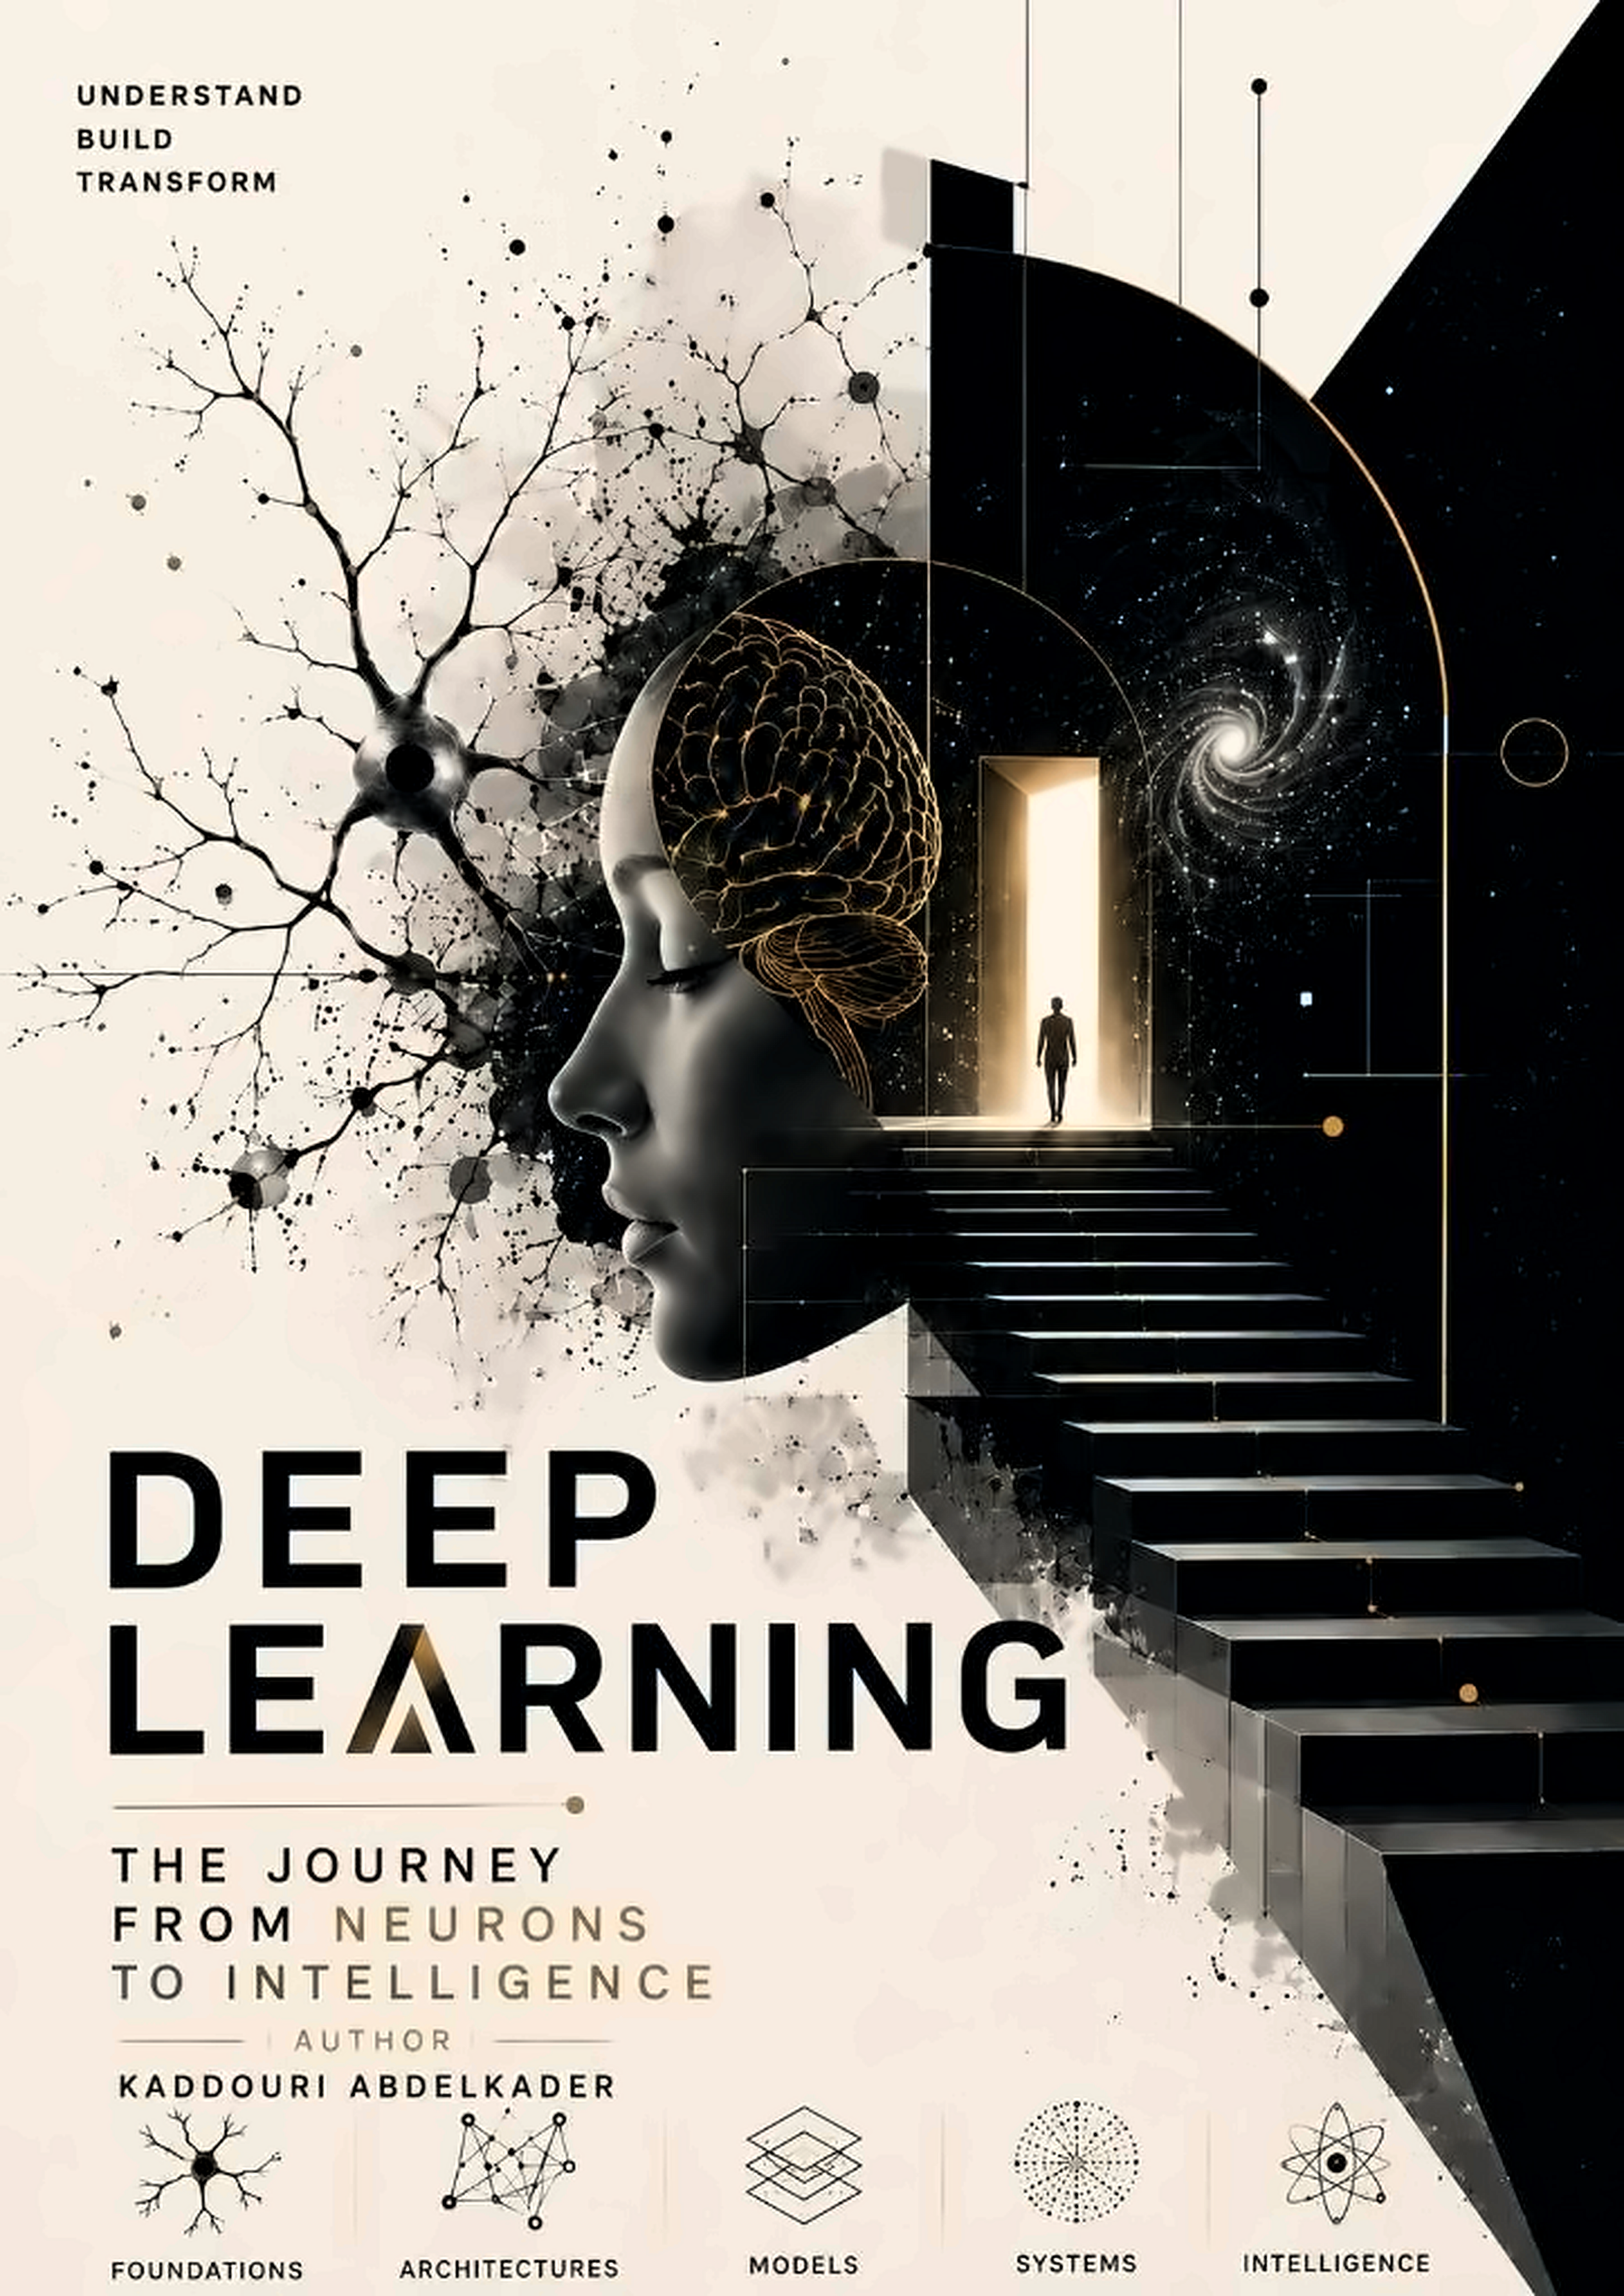
\includegraphics[width=\paperwidth,height=\paperheight]{figures/cover.png}%
    }%
  }%
  \null\clearpage
  \end{titlepage}%
}
\makeatother

% Hyperlinks
\usepackage{hyperref}
\hypersetup{
    colorlinks=true,
    linkcolor=primaryblue,
    citecolor=secondaryblue,
    urlcolor=secondaryblue,
    filecolor=primaryblue,
    menucolor=primaryblue,
    runcolor=primaryblue,
    pdfborder={0 0 0},
    pdfauthor={Kaddouri Abdelkader},
    pdftitle={Deep Learning: The Journey from Neurons to Intelligence}
}

\title{Deep Learning \\[0.55em] {\fontsize{18}{23}\selectfont The Journey from Neurons to Intelligence}}
\author{Kaddouri Abdelkader}
\date{\today}

\begin{document}

\frontmatter
\maketitle

\thispagestyle{empty}

\vspace*{\fill}

\begin{center}
    {\Large\textbf{Deep Learning: The Journey from Neurons to Intelligence}}
    
    \vspace{0.5cm}
    
    {\large\textit{Foundations, Architectures, and Modern AI}}
    
    \vspace{1.5cm}
    
    {\large\textbf{Copyright \textcopyright\ 2026 by Kaddouri Abdelkader}}
    
    \vspace{0.8cm}
    
    All rights reserved.
\end{center}

\vspace{1cm}

\noindent
No part of this publication may be reproduced, distributed, or transmitted
in any form or by any means, including photocopying, recording, or other
electronic or mechanical methods, without the prior written permission of
the copyright holder, except for brief quotations used for purposes such
as criticism, review, or scholarly reference.

\vspace{0.5cm}

\noindent
This book is intended for educational and informational purposes. While
every effort has been made to ensure the accuracy and clarity of the
material presented, the author makes no warranty, expressed or implied,
regarding the completeness or accuracy of the information contained in
this work. The field of artificial intelligence and deep learning evolves
rapidly, and some methods, tools, or technologies discussed in this book
may change over time.

\vspace{0.5cm}

\noindent
All product names, company names, trademarks, service marks, and other
registered names mentioned in this book belong to their respective owners.
Their use in this publication does not imply endorsement or affiliation.

\vspace{0.8cm}

\begin{center}
    \textbf{First Edition}\\[0.3cm]
    2026\\[0.8cm]
\end{center}

\vspace*{\fill}

\clearpage

\section*{Prerequisites}

To get the most out of \textit{Deep Learning: The Journey from Neurons to Intelligence}, readers are expected to have a basic understanding of mathematics and machine learning. The book develops the deep learning concepts progressively, so an advanced background is not required.

\subsection*{1. Mathematics Foundations}

A basic understanding of the following mathematical concepts is recommended:

\begin{itemize}
    \item \textbf{Linear Algebra:} Vectors, matrices, matrix multiplication, dot products, and vector spaces. These concepts are fundamental to understanding neural network layers, embeddings, and the matrix operations used in Transformer architectures.

    \item \textbf{Multivariable Calculus:} Derivatives, partial derivatives, gradients, and the chain rule. These concepts are essential for understanding backpropagation, gradient-based learning, and optimization.

    \item \textbf{Probability and Statistics:} Basic probability distributions, mean, variance, expectation, and related concepts. These provide useful foundations for understanding models such as Variational Autoencoders, Generative Adversarial Networks, and Diffusion Models.
\end{itemize}

\subsection*{2. Machine Learning Foundations}

Readers should be familiar with the basic terminology and principles of machine learning, including:

\begin{itemize}
    \item Supervised and unsupervised learning
    \item Training, validation, and test datasets
    \item Overfitting and underfitting
    \item Loss functions and optimization
    \item Hyperparameters
    \item Basic evaluation metrics such as accuracy and error
\end{itemize}

A detailed knowledge of machine learning algorithms is not required. The necessary concepts are introduced or revisited throughout the book when they become relevant to deep learning.

\subsection*{3. Domain Concepts}

The following background is helpful, but not strictly required:

\begin{itemize}
    \item \textbf{Computer Vision:} A basic understanding of how digital images are represented as grids of pixels, typically described by their height, width, and color channels (e.g., RGB).

    \item \textbf{Natural Language Processing (NLP):} A basic understanding that text can be represented as sequences of tokens, including words or subword units, and processed as numerical representations by neural networks.
\end{itemize}

\subsection*{A Note to the Reader}

You do not need to master all of these topics before starting the book. The goal of these prerequisites is simply to provide a foundation that will make the mathematical and technical concepts easier to follow. Whenever a concept is essential to understanding a later topic, the book introduces it at the point where it is needed.

\clearpage

\setcounter{tocdepth}{2}
\tableofcontents
\clearpage

\chapter*{Introduction to Deep Learning}

\section*{What Is Deep Learning?}

Deep Learning is a branch of machine learning that enables computers to learn complex patterns directly from data using artificial neural networks with multiple layers. Unlike traditional machine learning methods, which often rely on manually designed features, deep learning automatically learns useful representations from raw data during training. This ability has significantly improved the performance of intelligent systems across a wide range of applications.

The term \textit{deep} refers to the presence of multiple hidden layers within a neural network. Rather than solving a problem in a single step, each layer transforms its input into a more meaningful representation before passing it to the next layer. As information flows through the network, increasingly complex patterns are extracted, allowing the model to solve tasks that would be difficult using conventional algorithms.

One of the key strengths of deep learning is its ability to perform \textbf{representation learning}. Instead of requiring domain experts to manually identify the most informative features, the network automatically discovers the features that best describe the data. For example, in image recognition, the first layers typically detect simple visual patterns such as edges, while deeper layers combine these patterns to recognize objects. Similar hierarchical representations are learned in natural language processing and speech recognition.

The rapid progress of deep learning has been driven by several technological advances, including the availability of large datasets, powerful Graphics Processing Units (GPUs), and improved optimization algorithms. Together, these advances have enabled researchers to train neural networks containing millions or even billions of parameters, leading to remarkable improvements in accuracy and scalability.

Today, deep learning is a central component of many modern artificial intelligence systems. It is widely used in computer vision, speech recognition, natural language processing, recommender systems, autonomous driving, robotics, medical image analysis, and generative artificial intelligence. Modern AI also draws on symbolic methods, probabilistic methods, optimization, search, reinforcement learning, and hybrid systems. Although these applications employ different architectures, they all rely on the same fundamental principle: learning through artificial neural networks.

Before exploring these advanced architectures, it is essential to understand the basic computational model on which they are built. The fundamental building block of every deep learning model is the artificial neuron, which forms the basis of artificial neural networks.


\mainmatter
\chapter{Neural Networks}

\section{Biological Inspiration}

Artificial neural networks were inspired by the human brain, one of the most efficient information-processing systems found in nature. Although artificial neural networks are much simpler than biological brains, they were developed by adopting the basic principle of how biological neurons receive, process, and transmit information.

A biological neuron consists of three main components. The \textbf{dendrites} receive electrical signals from other neurons, the \textbf{cell body} (or soma) integrates these incoming signals, and the \textbf{axon} transmits the resulting signal to other neurons through specialized connections called synapses. A neuron generates an electrical impulse only when the combined incoming signals exceed a certain threshold, allowing information to propagate throughout the nervous system.

\begin{figure}[h]
    \centering
    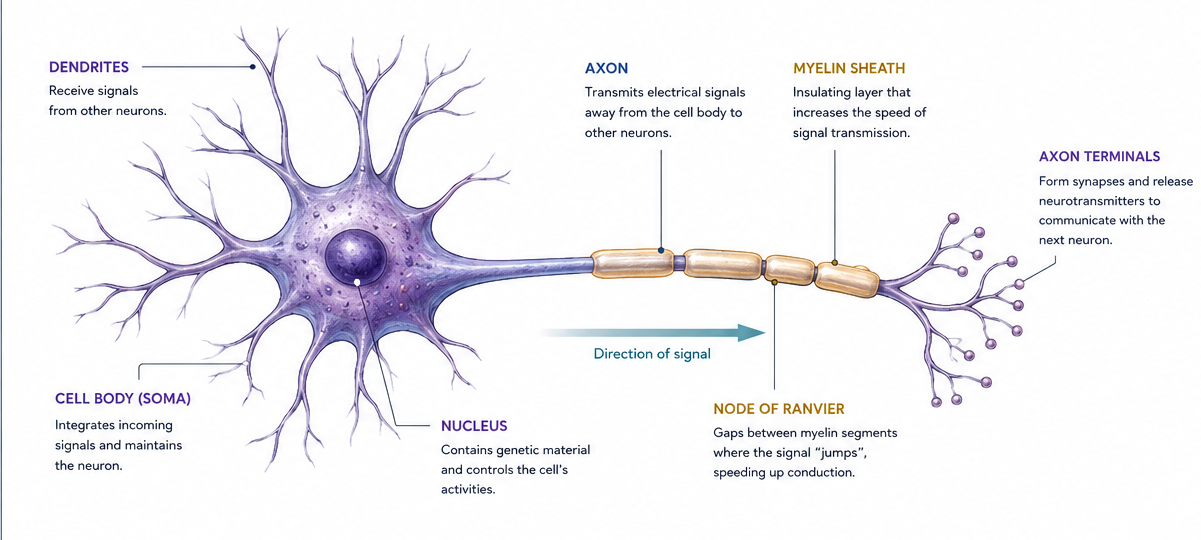
\includegraphics[width=0.95\textwidth]{figures/1-0.png}
\end{figure}
Inspired by this mechanism, Warren McCulloch and Walter Pitts proposed the first mathematical model of an artificial neuron in 1943. Although highly simplified, their model demonstrated that a neuron could be represented as a computational unit capable of receiving multiple inputs, combining them, and producing an output. This work laid the foundation for the development of artificial neural networks.

It is important to note that artificial neurons are not intended to accurately replicate the biological brain. Instead, they capture only its essential computational principle: combining multiple inputs to produce an output. This simple idea forms the basis of all modern neural network architectures.


\section{Artificial Neural Networks}

Artificial Neural Networks (ANNs) are computational models composed of interconnected processing units called \textbf{artificial neurons}. Inspired by the structure of the human brain, these networks are designed to learn relationships between input data and desired outputs by adjusting their internal parameters during training.

An artificial neural network is organized into layers of neurons through which information flows sequentially. Each neuron receives information from neurons in the previous layer, performs a simple mathematical computation, and passes its output to the next layer. By combining the outputs of many interconnected neurons, the network is capable of solving increasingly complex problems.

A typical feedforward neural network consists of three types of layers:

\begin{itemize}
    \item \textbf{Input Layer:} Receives the input features from the dataset.
    \item \textbf{Hidden Layer(s):} Process the information and extract increasingly meaningful representations.
    \item \textbf{Output Layer:} Produces the final prediction of the network.
\end{itemize}

The basic computational unit of the network is the artificial neuron. Each neuron receives one or more input values, combines them using trainable parameters called \textbf{weights}, adds a \textbf{bias} term, and computes

\begin{equation}
z=\sum_{i=1}^{n}w_i x_i+b.
\end{equation}

The computed value is then passed through an \textbf{activation function}, which determines the neuron's output. By connecting many neurons together, the network can gradually transform raw input data into increasingly useful representations.

During training, the network automatically adjusts its weights and biases to minimize prediction errors. As a result, the network gradually learns the relationship between the input data and the desired output.

The simplest neural network consists of a single artificial neuron and is known as the \textbf{Perceptron}. Although simple, the Perceptron introduced the fundamental principles upon which modern deep learning models are built.
\section{Perceptron}

The \textbf{Perceptron} is the simplest form of an artificial neural network and the first computational model capable of learning from data. Proposed by Frank Rosenblatt in 1958, it extended the earlier McCulloch--Pitts neuron by introducing a learning mechanism that automatically adjusts its parameters using training examples. This innovation marked an important milestone in the development of machine learning and laid the foundation for modern neural networks.

A Perceptron consists of a single artificial neuron that receives one or more input values and produces a binary output. Like every artificial neuron, it combines the inputs using trainable weights, adds a bias term, and computes a weighted sum given by

\begin{equation}
z=\sum_{i=1}^{n}w_i x_i+b.
\end{equation}

The weighted sum is then passed through a \textbf{threshold activation function}, also known as the step function, which determines the final output:
\clearpage
\begin{equation}
\hat{y}=
\begin{cases}
1, & z \geq 0,\\
0, & z < 0.
\end{cases}
\end{equation}

\begin{figure}[h]
    \centering
    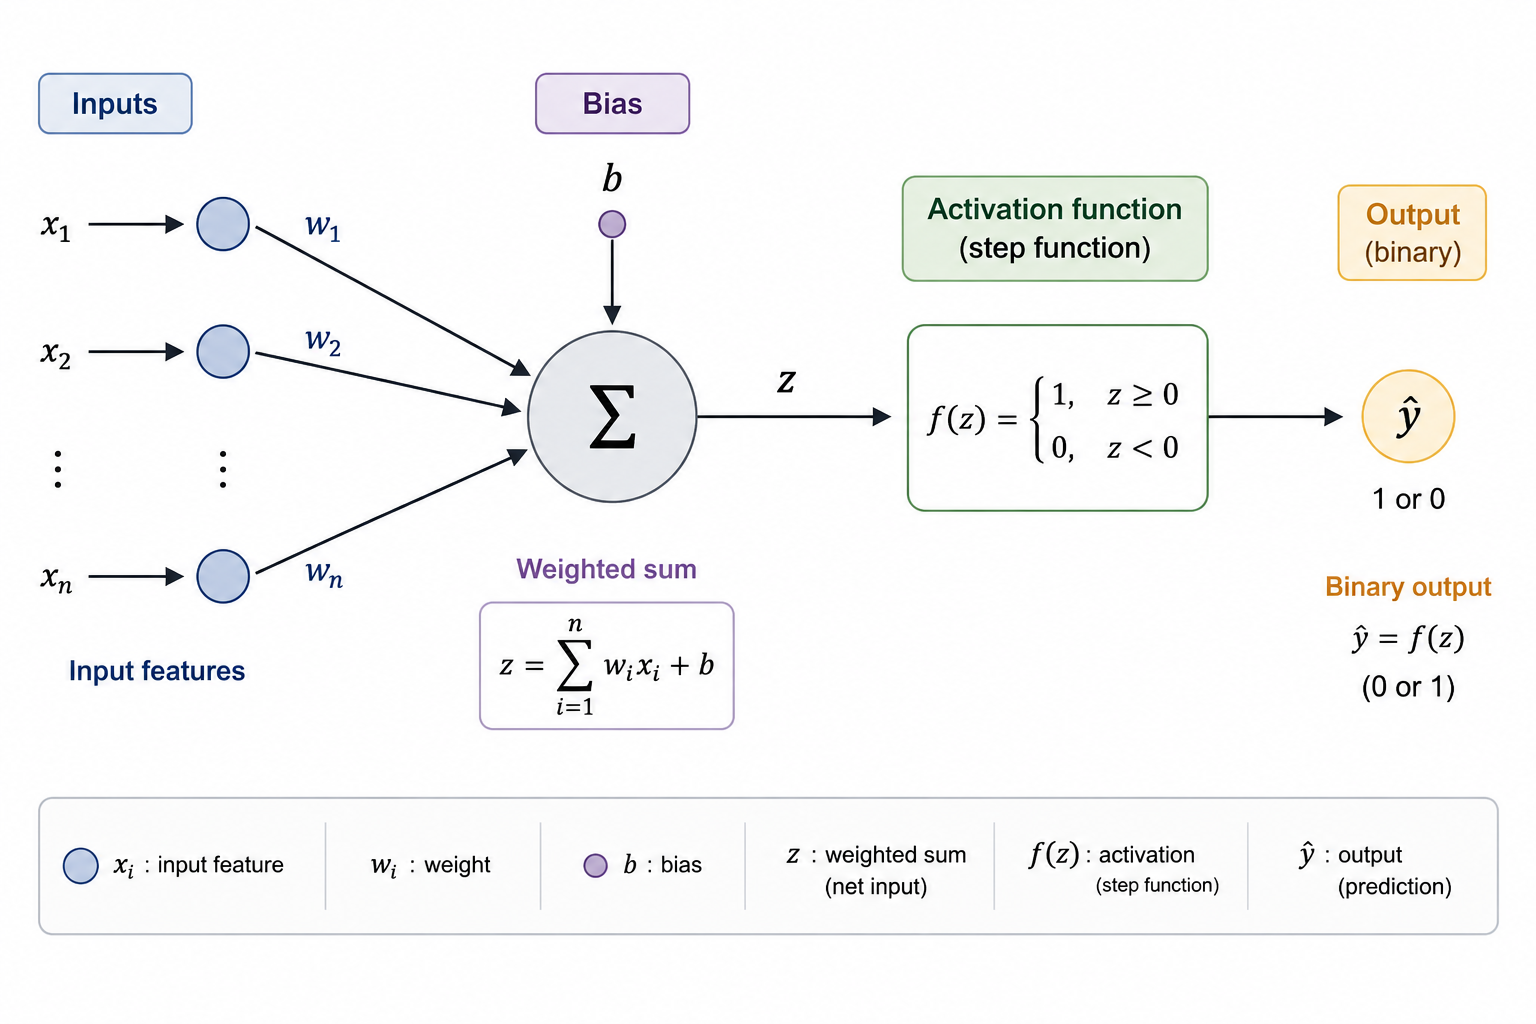
\includegraphics[width=0.95\textwidth]{figures/1-1.png}
\end{figure}

The Perceptron is therefore a \textbf{binary classifier}, meaning that it can assign an input to one of two possible classes. Geometrically, it does so by learning a \textbf{linear decision boundary} that separates the classes. In two-dimensional space, this boundary is represented by a straight line; in higher dimensions, it is referred to as a hyperplane.
\begin{figure}[h]
    \centering
    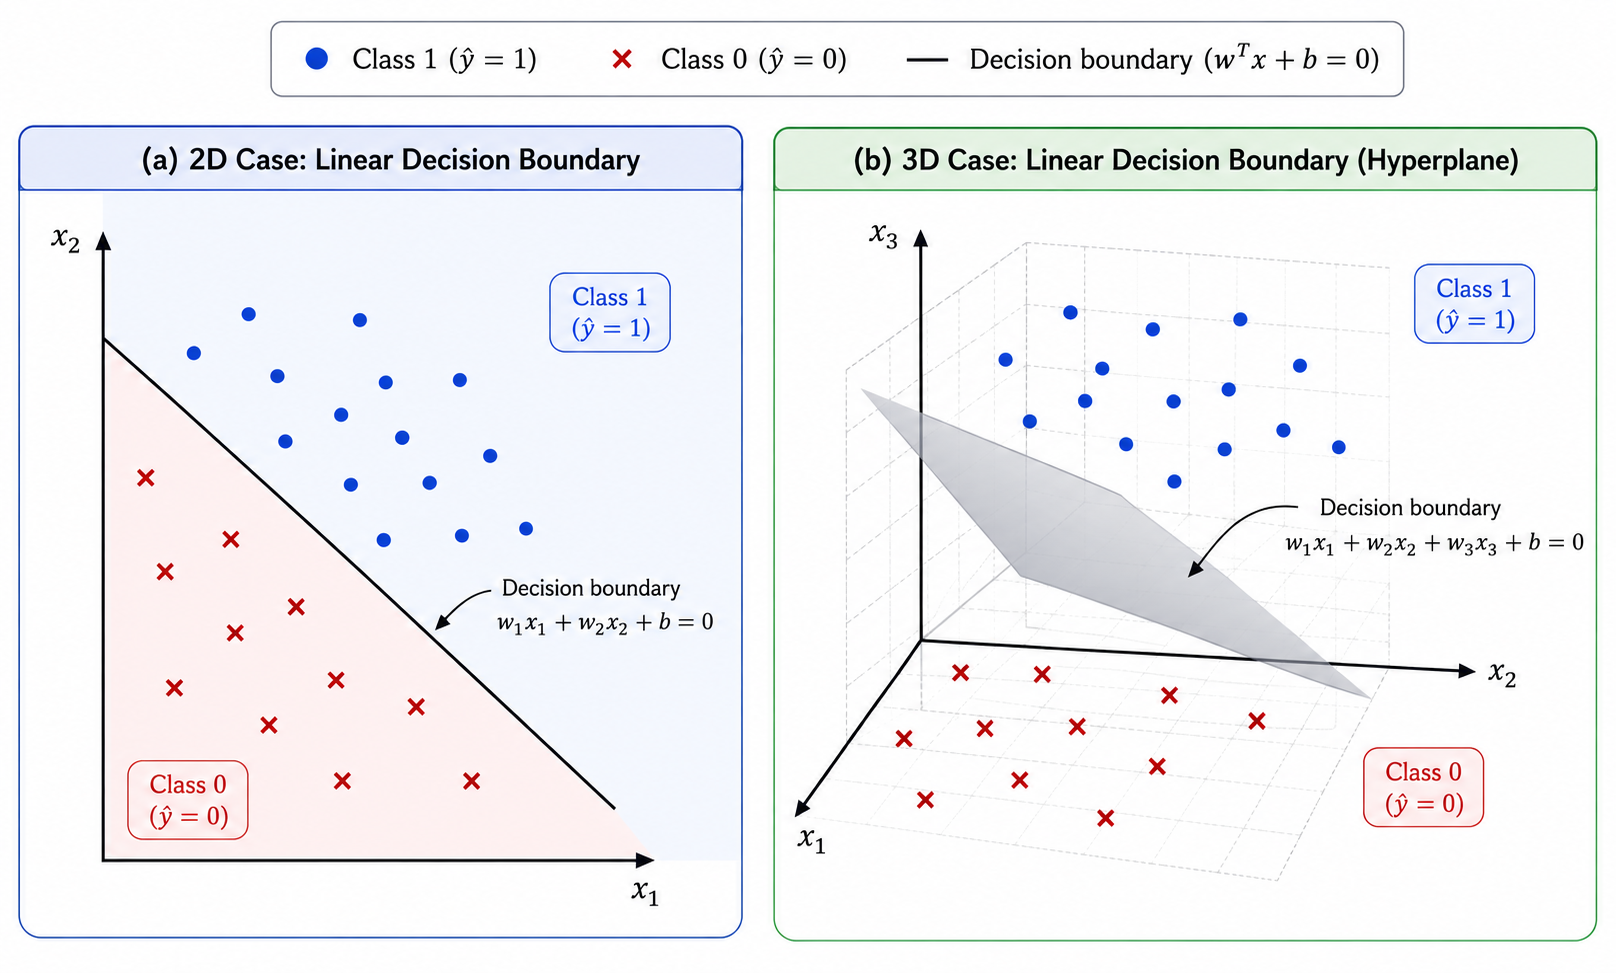
\includegraphics[width=0.95\textwidth]{figures/first.png}
\end{figure}
Despite its simplicity, the Perceptron introduced several fundamental concepts that remain at the core of modern deep learning, including trainable parameters, prediction, and learning from data. 
\section{Perceptron Learning Algorithm}

The distinguishing feature of the Perceptron is its ability to learn automatically from data. Rather than manually selecting the values of the weights and bias, the Perceptron adjusts these parameters during training so that its predictions become increasingly accurate. This process is known as the \textbf{Perceptron Learning Algorithm}.

The algorithm begins by initializing the weights and bias, typically with small random values or zeros. The training dataset is then presented to the model one example at a time. For each training sample, the Perceptron computes the weighted sum, applies the threshold activation function, and produces a predicted output.

The prediction is compared with the true class label to determine whether the classification is correct. If the prediction is correct, no changes are made to the model parameters. Otherwise, the weights and bias are updated according to the Perceptron learning rule.

Let $y$ denote the true class label and $\hat{y}$ the predicted output. The prediction error is defined as

\begin{equation}
e = y - \hat{y}.
\end{equation}

The weights are updated using

\begin{equation}
w_i \leftarrow w_i + \eta e x_i,
\end{equation}

while the bias is updated as

\begin{equation}
b \leftarrow b + \eta e,
\end{equation}

where $\eta$ is the \textbf{learning rate}, a positive constant that controls the magnitude of each update.

This procedure is repeated for all training samples. After one complete pass through the dataset, called an \textbf{epoch}, the algorithm starts another pass using the updated parameters. Training continues until the Perceptron correctly classifies all training examples or until a predefined number of epochs is reached.
\vspace{3cm}
The complete learning procedure can be summarized as follows:
\clearpage
\begin{figure}[h]
    \centering
    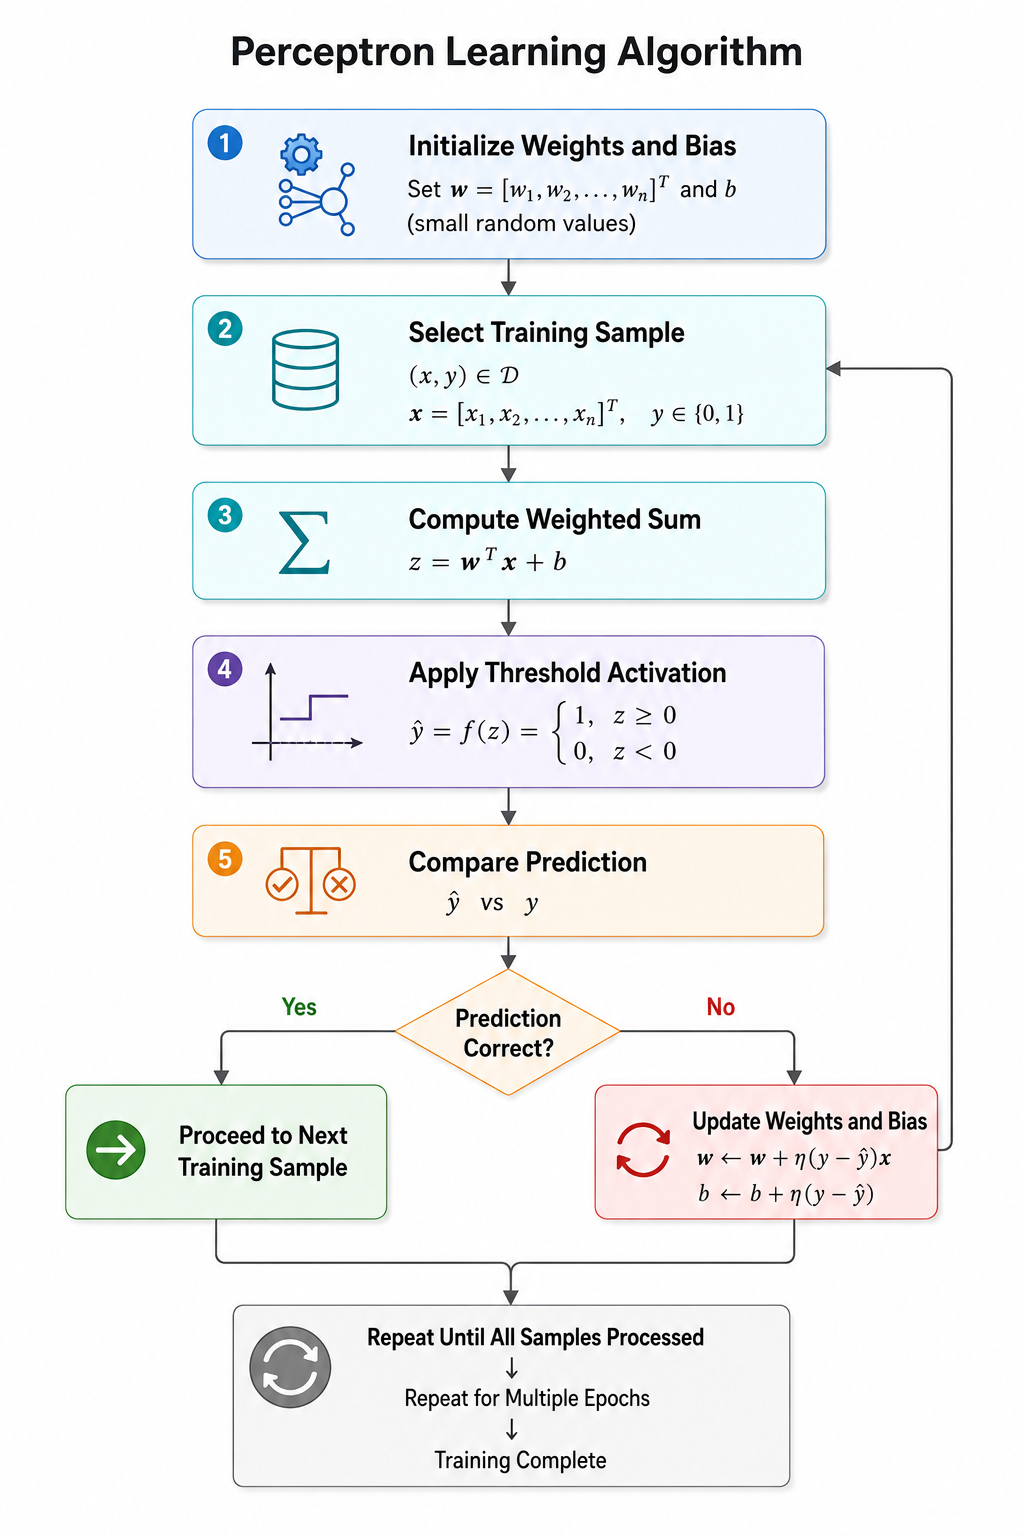
\includegraphics[width=0.95\textwidth]{figures/1-3 figure.png}
\end{figure}
\clearpage

An important property of the Perceptron Learning Algorithm is described by the \textbf{Perceptron Convergence Theorem}, which states that if the training data are linearly separable, the algorithm is guaranteed to find a decision boundary after a finite number of updates. However, when the data are not linearly separable, the algorithm cannot converge to a perfect solution. This limitation motivates the study of one of the most famous problems in the history of neural networks: the XOR problem.

\section{The XOR Problem}

Although the Perceptron was a significant breakthrough in the development of artificial neural networks, it has an important limitation: it can correctly classify only \textbf{linearly separable} data. A dataset is said to be linearly separable if its classes can be separated by a single straight line (or, more generally, by a hyperplane).

One of the simplest examples of a non-linearly separable problem is the \textbf{Exclusive OR (XOR)} logical function. The XOR function produces an output of 1 only when its two inputs are different, as shown in Table~\ref{tab:xor}.

\begin{table}[h]
\centering
\caption{Truth table of the XOR function.}
\label{tab:xor}
\begin{tabular}{ccc}
\hline
$x_1$ & $x_2$ & XOR \\
\hline
0 & 0 & 0 \\
0 & 1 & 1 \\
1 & 0 & 1 \\
1 & 1 & 0 \\
\hline
\end{tabular}
\end{table}
\begin{figure}[h]
    \centering
    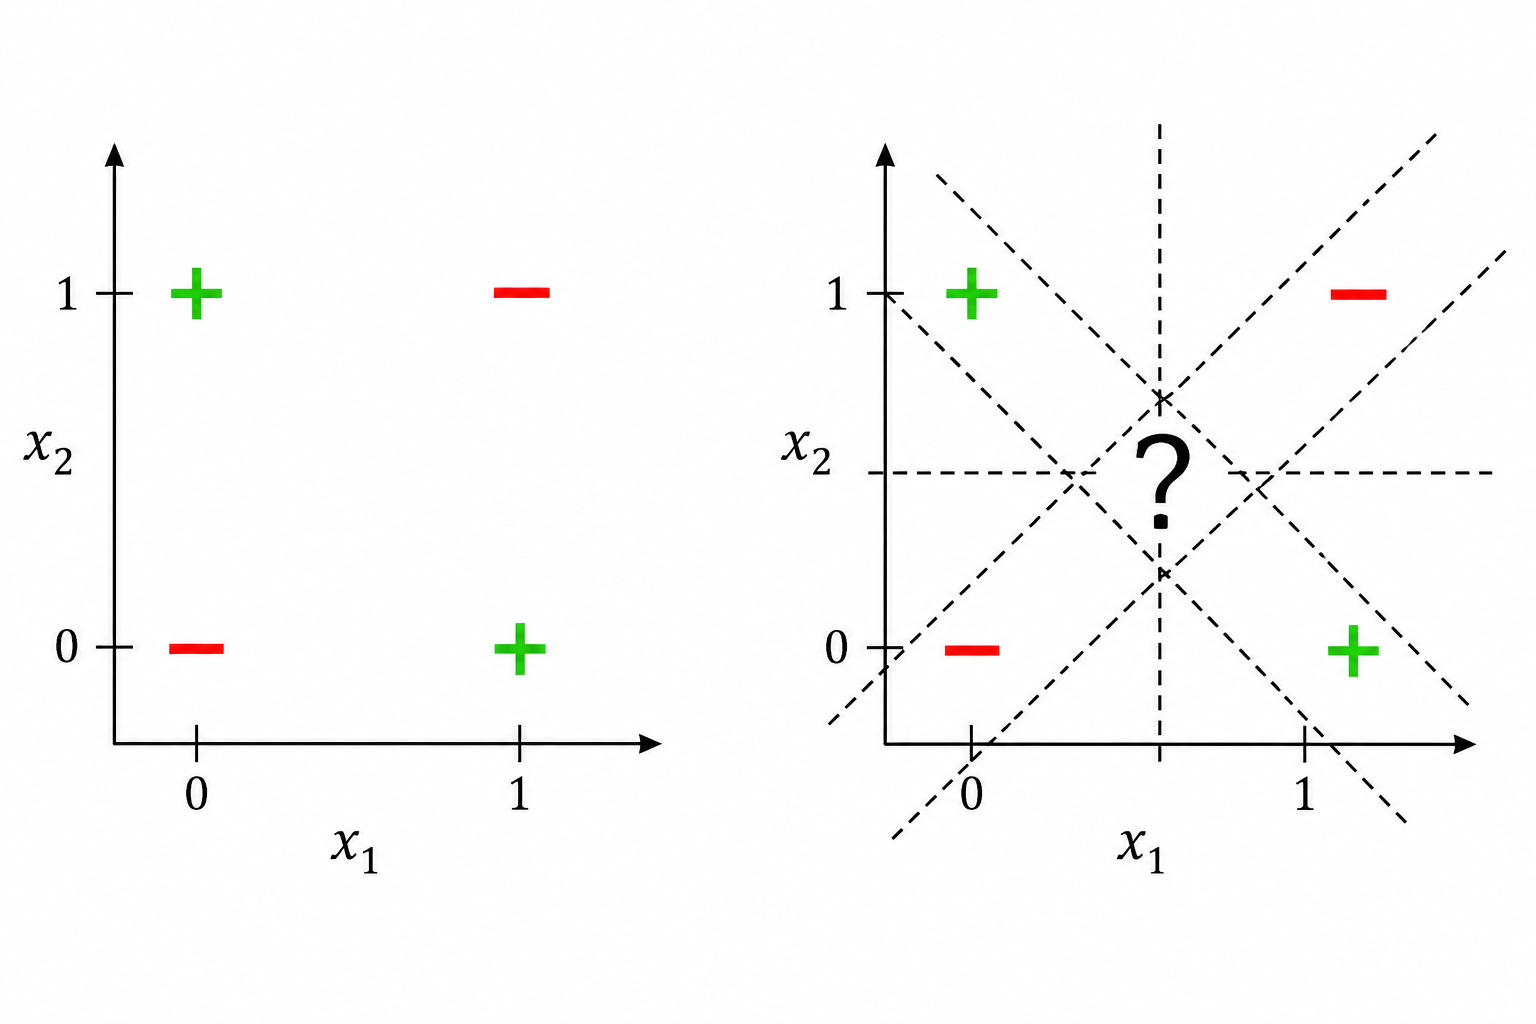
\includegraphics[width=0.95\textwidth]{figures/1-4.png}
\end{figure}

When these four input combinations are represented in a two-dimensional plane, no single straight line can separate the two classes. Since the Perceptron always learns a linear decision boundary, it is mathematically impossible for a single-layer Perceptron to solve the XOR problem.

This limitation was highlighted by Marvin Minsky and Seymour Papert in their influential 1969 book \textit{Perceptrons}. Their work demonstrated that single-layer neural networks are unable to represent certain simple functions, including XOR. As a result, research on neural networks declined for several years, a period that is often referred to as the \textbf{AI Winter}.

The XOR problem also revealed an important insight: some problems require models capable of learning \textbf{non-linear decision boundaries}. This challenge was eventually overcome by introducing one or more hidden layers between the input and output layers, giving rise to the \textbf{Multi-Layer Perceptron (MLP)}.

\section{Multi-Layer Perceptron (MLP)}

The limitations of the single-layer Perceptron motivated the development of more powerful neural network architectures capable of learning complex, non-linear relationships. The simplest extension is the \textbf{Multi-Layer Perceptron (MLP)}, which introduces one or more hidden layers between the input and output layers.

An MLP is a feedforward neural network composed of multiple layers of interconnected neurons. Information flows sequentially from the input layer through one or more hidden layers until it reaches the output layer. Each neuron performs the same basic computation introduced in the previous sections, while the hidden layers progressively transform the input into increasingly meaningful representations.

The addition of hidden layers greatly increases the expressive power of the network. Unlike a single-layer Perceptron, which can learn only linear decision boundaries, an MLP is capable of modeling highly complex and non-linear functions. This enables it to solve problems such as the XOR classification task and forms the basis of many modern deep learning models.

Figure~\ref{fig:mlp_architecture} illustrates the general architecture of a Multi-Layer Perceptron. The input layer receives the features from the dataset and passes them to the first hidden layer. Each hidden neuron computes a weighted sum of its inputs, adds a bias term, and produces an output that is forwarded to the next layer. This process continues through all hidden layers until the output layer generates the network's final prediction.

\begin{figure}[h]
    \centering
    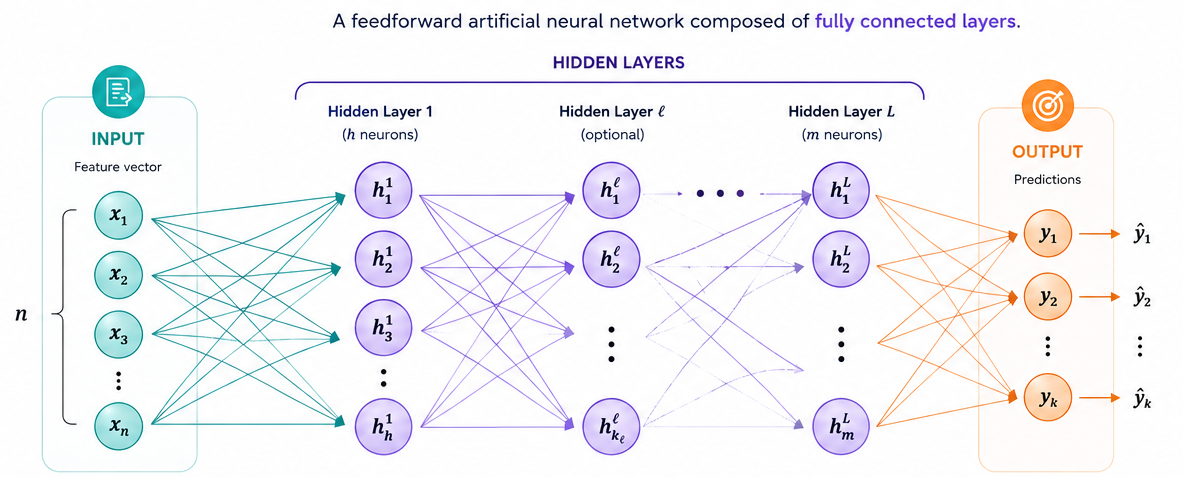
\includegraphics[width=0.95\textwidth]{figures/1-5.png}
    \caption{Architecture of a Multi-Layer Perceptron (MLP).}
    \label{fig:mlp_architecture}
\end{figure}
Although the architecture of an MLP is conceptually simple, stacking multiple layers alone is not sufficient to increase the network's learning capability. If every neuron performed only a linear transformation, the entire network would still behave as a single linear model, regardless of the number of hidden layers. To overcome this limitation, each neuron applies an \textbf{activation function}, introducing the non-linearity that enables deep neural networks to learn complex patterns.


\section{Activation Functions}

Without activation functions, a deep neural network is equivalent to a single layer.

Activation functions introduce non-linearity, allowing the network to approximate complex functions.

An ideal activation function should:
\begin{itemize}
    \item Introduce non-linearity (curved and complex decision boundaries, not just a straight line)
    \item Be differentiable (or almost everywhere differentiable)
    \item Be computationally efficient
    \item Avoid vanishing gradient
    \item Avoid exploding gradient
    \item Have a stable output range
\end{itemize}

\subsection{Sigmoid}

\begin{equation}
\sigma(x) = \frac{1}{1 + e^{-x}} \qquad \text{Range: } (0, 1)
\end{equation}

\sigmoidplot

Output values that resemble probabilities (e.g., $0.98 \to \text{very likely}$, $0.5 \to \text{uncertain}$, $0.02 \to \text{very unlikely}$).

\begin{advbox}[Sigmoid Summary]
\textbf{Advantages:}
\begin{itemize}
    \item Smooth and differentiable.
    \item Output interpretable as a probability.
    \item Works well for binary classification outputs.
\end{itemize}

\tcbline

\textbf{Disadvantages:}
\begin{itemize}
    \item \textbf{Vanishing Gradient:} For very large positive or negative inputs, $\sigma'(x) \approx 0$. The gradient becomes extremely small, slowing or stopping learning in deep networks.
    \item \textbf{Saturation:}
    \begin{equation}
    \text{For } x \gg 0, \quad \sigma(x) \approx 1; \qquad \text{For } x \ll 0, \quad \sigma(x) \approx 0
    \end{equation}
    Small changes in input barely affect the output.
    \item \textbf{Not Zero-Centered:} Outputs are always positive, which can lead to less efficient optimization because gradients tend to have the same sign.
\end{itemize}
\end{advbox}

\paragraph{Usage:}
\begin{itemize}
    \item \textbf{Hidden Layer:} Rarely used.
    \item \textbf{Output Layer:} Binary classification.
\end{itemize}

\subsection{Tanh (Hyperbolic Tangent)}

\begin{equation}
\tanh(x) = \frac{e^x - e^{-x}}{e^x + e^{-x}} \qquad \text{Range: } (-1, 1)
\end{equation}

\begin{equation}
\text{Derivative: } 1 - \tanh^2(x)
\end{equation}

\tanhplot

\begin{advbox}[Tanh Summary]
\textbf{Advantages:}
\begin{itemize}
    \item \textbf{Zero-Centered:} Output can be positive or negative. This generally leads to faster convergence than Sigmoid.
    \item \textbf{Larger Gradient Near Zero:} Learning is often faster around the origin.
\end{itemize}

\tcbline

\textbf{Disadvantages:}
\begin{itemize}
    \item \textbf{Vanishing Gradients.}
    \item \textbf{Saturation for large positive and negative $x$:}
    \begin{align*}
        10 &\rightsquigarrow 1 & 50 &\rightsquigarrow 1 \\
        100 &\rightsquigarrow 1 & 1000 &\rightsquigarrow 1 \\
        10 \times 10^{50} &\rightsquigarrow 1 & -10 \times 10^{50} &\rightsquigarrow -1
    \end{align*}
\end{itemize}
\end{advbox}

\paragraph{Usage:} Common in RNNs; less common in modern feed-forward networks.

\subsection{ReLU (Rectified Linear Unit)}

\begin{equation}
f(x) = \max(0, x) \qquad \text{Range: } [0, +\infty)
\end{equation}

\begin{equation}
\text{Derivative: } f'(x) = \begin{cases} 1 & x > 0 \\ 0 & x < 0 \end{cases}
\end{equation}
\reluplot
\textit{Note: At $x = 0$, $f'(0)$ is non-differentiable. Most Python frameworks define it as 0 or 1.}

\begin{advbox}[ReLU Summary]
\textbf{Advantages:}
\begin{itemize}
    \item \textbf{Extremely Fast:} Only requires a comparison with zero.
    \item \textbf{Sparse Activation:} Negative inputs become exactly zero, making many neurons inactive (improves efficiency and sometimes reduces overfitting).
    \item \textbf{Reduces Vanishing Gradient:} For positive inputs, $f'(x) = 1$. The gradient passes through unchanged.
\end{itemize}

\tcbline

\textbf{Disadvantages:}
\begin{itemize}
    \item \textbf{Dying ReLU:} If a neuron's output becomes permanently negative ($f(x) = 0$), its gradient is also zero, so the neuron may never recover.
    \item \textbf{Unbounded Output:} Large activations can sometimes contribute to exploding activation if not managed properly.
\end{itemize}
\end{advbox}

\paragraph{Usage:} The default choice for hidden layers in many neural networks, including CNNs and MLPs.

\subsection{Leaky ReLU \& Parametric ReLU (PReLU)}

\begin{equation}
f(x) = \begin{cases} x & x > 0 \\ \alpha x & x < 0 \end{cases}, \qquad \alpha = 0.01 \qquad \text{Range: } (-\infty, +\infty)
\end{equation}

\begin{equation}
f'(x) = \begin{cases} 1 & x > 0 \\ \alpha & x < 0 \end{cases}
\end{equation}

\leakyreluplot

Invented to solve the Dying ReLU problem by allowing a small, non-zero gradient when the input is negative.

\begin{advbox}[Leaky ReLU Summary]
\textbf{Advantages:}
\begin{itemize}
    \item Reduces the chance of dead neurons.
    \item Still computationally efficient.
    \item Preserves gradient flow for negative inputs.
\end{itemize}

\tcbline

\textbf{Disadvantages:}
\begin{itemize}
    \item Introduces a hyperparameter ($\alpha$).
    \item Usually offers only modest improvements over ReLU.
\end{itemize}
\end{advbox}

\paragraph{Usage:} Used when standard ReLU leads to many dead neurons.

\paragraph{Parametric ReLU (PReLU):} Instead of fixing $\alpha$, the network learns it during training ($\alpha$ is a trainable parameter).
\begin{itemize}
    \item \textbf{Range:} $(-\infty, +\infty)$
    \item \textbf{Usage:} Sometimes used in computer vision models.
\end{itemize}

\subsection{ELU (Exponential Linear Unit)}

\begin{equation}
f(x) = \begin{cases} x & x > 0 \\ \alpha(e^x - 1) & x \le 0 \end{cases} \qquad \text{Range: } (-\infty, +\infty)
\end{equation}

\eluplot

\begin{advbox}[ELU Summary]
\textbf{Advantages:}
\begin{itemize}
    \item Smooth transition near zero.
    \item Negative outputs are allowed, making activations closer to zero-centered.
    \item Can converge faster than ReLU in some settings.
\end{itemize}

\tcbline

\textbf{Disadvantages:}
\begin{itemize}
    \item More computationally expensive because it uses the exponential function.
    \item Still has a saturation region for very negative inputs.
\end{itemize}
\end{advbox}

\paragraph{Usage:} Sometimes used instead of ReLU, though less common today.

\subsection{GELU (Gaussian Error Linear Unit)}

\begin{equation}
\text{GELU}(x) = x \Phi(x) \qquad \text{Range: } (-\infty, +\infty)
\end{equation}
where $\Phi(x)$ is the Cumulative Distribution Function (CDF) of the standard normal distribution.

A common approximation is:
\begin{equation}
\text{GELU}(x) \approx 0.5x \left( 1 + \tanh\left( \sqrt{\frac{2}{\pi}} \left( x + 0.044715 x^3 \right) \right) \right)
\end{equation}

\geluplot

Unlike ReLU, which either keeps or discards an input, GELU smoothly scales the input based on its magnitude.

\begin{advbox}[GELU Summary]
\textbf{Advantages:}
\begin{itemize}
    \item Smooth and differentiable.
    \item Excellent empirical performance in Transformers.
    \item Often leads to better accuracy than ReLU in language models.
\end{itemize}

\tcbline

\textbf{Disadvantages:}
\begin{itemize}
    \item Computationally more expensive than ReLU.
    \item Harder to compute analytically.
\end{itemize}
\end{advbox}

\paragraph{Usage:} Widely used in Transformer architectures, including models like BERT and GPT.

\subsection{Softmax}

For outputs $z_1, z_2, \dots, z_K$:
\begin{equation}
\text{Softmax}(z_i) = \frac{e^{z_i}}{\sum_{j=1}^{K} e^{z_j}}
\end{equation}

\softmaxplot

\begin{propertybox}[Softmax Properties]
\begin{itemize}
    \item Every output is between 0 and 1, and $\sum_{i=1}^K \text{Softmax}(z_i) = 1$.
    \item Produces a probability distribution over classes.
\end{itemize}
\end{propertybox}

\begin{advbox}[Softmax Summary]
\textbf{Advantages:}
\begin{itemize}
    \item Ideal for multi-class classification.
    \item Easy to interpret probabilistically.
\end{itemize}

\tcbline

\textbf{Disadvantages:}
\begin{itemize}
    \item Computationally expensive for very large numbers of classes.
    \item Can become numerically unstable if implemented naively.
\end{itemize}
\end{advbox}

\paragraph{Usage:} Always in the output layer for multi-class classification.

\subsection{Activation Selection Summary}

\begin{table}[h!]
\centering
\caption{Common Activation Functions by Network Type}
\begin{tabular}{ll}
\toprule
\textbf{Architecture / Task} & \textbf{Common Activation Function} \\
\midrule
MLP or CNN & ReLU or Leaky ReLU (if dead neurons occur) \\
Transformer Models & GELU, SwiGLU, or SiLU \\
Binary Classification & Sigmoid \\
Multi-Class Classification & Softmax (or logits with cross-entropy loss) \\
RNN & Tanh \\
\bottomrule
\end{tabular}
\end{table}

\clearpage

\section{Forward Propagation, Backpropagation \& Training Dynamics}

\subsection{Forward Propagation}

Moving information from input toward output: $x \rightsquigarrow \hat{y}$.

Forward propagation is the process by which a Multi-Layer Perceptron (MLP) transforms an input vector into a prediction by passing information sequentially from the input layer to the output layer. Given an input vector $x$, each neuron in the first hidden layer computes a weighted sum of its inputs followed by the addition of a bias term:
\begin{equation}
z^{(1)} = W^{(1)} x + b^{(1)}
\end{equation}

After that, we pass it into an activation function to produce (non-linear) hidden layer activations:
\begin{equation}
a^{(1)} = f\left(z^{(1)}\right)
\end{equation}

The activation function introduces non-linearity into the network, enabling it to learn complex relationships between the input feature and the target output. The output of one layer becomes the input to the next layer, and this process is repeated for every hidden layer $l$:
\begin{align}
z^{(l)} &= W^{(l)} a^{(l-1)} + b^{(l)} \\
a^{(l)} &= f\left(z^{(l)}\right)
\end{align}

After propagating through all hidden layers, we apply the output activation function to generate the network's prediction $\hat{y}$:
\begin{equation}
\hat{y} = g\left(z^{(L)}\right)
\end{equation}
where $g(\cdot)$ depends on the learning task:
\begin{itemize}
    \item \textbf{For binary classification:} Sigmoid function
    \item \textbf{For multi-class classification:} Softmax
    \item \textbf{For regression problems:} Any linear function
\end{itemize}

After we get $\hat{y}$ (prediction), it is compared with the true target $y$ using a loss function such as:
\begin{itemize}
    \item \textbf{MSE} (for regression)
    \item \textbf{Cross-Entropy Loss} (for categorical):
    \begin{equation}
    L = -\sum_{i} y_i \log(p_i)
    \end{equation}
    where $y_i$ is the one-hot encoded true label and $p_i$ is the probability from Softmax.
\end{itemize}
It measures how different the predicted probabilities are from the true labels.

\subsection{Backward Propagation}

Used to optimize the parameters of a Multilayer Perceptron (MLP) by minimizing the prediction error. After forward propagation, the network evaluates the discrepancy between $\hat{y}$ and $y$ using a loss function (MSE or Cross-Entropy). The objective of backward propagation is to determine how much each weight and bias contributed to this error and to compute the gradients required for updating the network parameters. This is accomplished using the \textbf{Chain Rule} of differential calculus, which allows the gradient of the loss function to be propagated backward from the output layer to the input layer.

\paragraph{Chain Rule:} If a function is composed of several nested functions $L = f(g(h(x)))$, the derivative of $L$ with respect to $x$ is obtained by multiplying each intermediate derivative:
\begin{equation}
\frac{\partial L}{\partial x} = \frac{\partial L}{\partial f} \cdot \frac{\partial f}{\partial g} \cdot \frac{\partial g}{\partial h} \cdot \frac{\partial h}{\partial x}
\end{equation}

To illustrate this concept, consider a single neuron with:
\begin{align}
z &= w x + b \\
a &= f(z) \\
\text{Loss: } L &= L(a)
\end{align}

\begin{equation}
\frac{\partial L}{\partial w} = \frac{\partial L}{\partial a} \cdot \frac{\partial a}{\partial z} \cdot \frac{\partial z}{\partial w}
\end{equation}

After calculating the gradients for all layers, the network updates its parameters using an optimization algorithm such as Gradient Descent. The weights and biases are adjusted in the direction that minimizes the loss according to the update rules:
\begin{align}
w_{\text{new}}^{(l)} &= w_{\text{old}}^{(l)} - \eta \frac{\partial L}{\partial w^{(l)}} \\
b_{\text{new}}^{(l)} &= b_{\text{old}}^{(l)} - \eta \frac{\partial L}{\partial b^{(l)}}
\end{align}
where $\eta$ is the learning rate.

\subsection{Vanishing Gradient Problem}

The vanishing gradient problem is one of the most significant challenges encountered when training deep neural networks using the backpropagation algorithm. It occurs when the gradients of the loss function with respect to the network parameters become progressively smaller as they are propagated backward from the output layer to the earlier hidden layers. As a result, the weights of neurons located near the input layer receive extremely small updates, preventing them from learning meaningful features. Consequently, the training process becomes very slow or may even stop entirely, leading to poor model performance and difficulty in optimizing deep neural networks.

The origin of the vanishing gradient problem lies in the repeated application of the chain rule during backpropagation.

For example, suppose each derivative has an average value of $0.5$. For a network with 10 hidden layers, the gradient becomes:
\begin{equation}
0.5^{10} = 0.00097
\end{equation}
For 20 hidden layers:
\begin{equation}
0.5^{20} = 9.54 \times 10^{-7}
\end{equation}
which is practically zero. The weight updates computed using Gradient Descent:
\begin{equation}
w_{\text{new}} = w_{\text{old}} - \eta \frac{\partial L}{\partial w}
\end{equation}
become extremely small because $\frac{\partial L}{\partial w} \approx 0$. The weights remain unchanged during training, and the network fails to learn useful representations.

The vanishing gradient problem is particularly severe when using activation functions whose derivatives are bounded between $0$ and $1$, such as Sigmoid and Tanh.

ReLU has a derivative equal to $1$ for positive inputs, allowing gradients to propagate through many layers without rapidly shrinking. That is why ReLU has become the standard activation function for most deep neural networks.

\subsection{Exploding Gradient Problem}

The exploding gradient problem occurs during backpropagation when gradients become excessively large as they propagate from the output layer to the earlier layers. Unlike the vanishing gradient producing excessively small weight updates, exploding gradients increase exponentially, producing excessively large weight updates that destabilize training. This often causes the loss to oscillate, diverge, or produce numerical overflow ($\infty$ or NaN), preventing the network from converging.

The exploding gradient problem arises from the repeated application of the chain rule during backpropagation.

For example:
\begin{equation}
2^{10} = 1024 \quad \rightsquigarrow \quad 2^{20} = 1048576
\end{equation}

Large weight values can further amplify this effect during forward propagation.

\begin{examplebox}[Exploding Update Example]
Suppose $w = 0.8$, $\eta = 0.01$, and $\frac{\partial L}{\partial w} = 5000$. Then:
\begin{equation}
w_{\text{new}} = 0.8 - 0.01 \times 5000 = -49.2
\end{equation}
Instead of a small adjustment, the weight changes from $0.8$ to $-49.2$ in a single update. Such a drastic modification significantly alters network behavior, creating a cycle of numerical instability.
\end{examplebox}

\paragraph{Mitigation Techniques:}
\begin{itemize}
    \item \textbf{Gradient Clipping:} Limit the magnitude of the gradient before updating the parameters by setting a threshold $c$.
    \item \textbf{Proper Weight Initialization:} Such as Xavier (Glorot) initialization.
    \item \textbf{Adaptive Optimization Algorithms:} Such as Adam and RMSProp.
\end{itemize}

\subsection{Heuristics for Hidden Layer Neurons}

Best heuristics used to initialize the number of neurons in hidden layers:

Between the input and output sizes ($N_o < N_h < N_i$):
\begin{itemize}
    \item \textbf{Two-Thirds Rule:}
    \begin{equation}
    N_h = \frac{2}{3} N_i + N_o \qquad (\text{most common})
    \end{equation}
    \item \textbf{Average Rule:}
    \begin{equation}
    N_h = \frac{N_i + N_o}{2}
    \end{equation}
    \item \textbf{Start Small and Increase Gradually:} $N_h = \{16, 32, 64, 128, \dots\}$
    \item \textbf{Grid Search:} Test all combinations $\{32, 64, 128\}$ and learning rates $\{0.1, 0.01, 0.001\}$ across 3 hidden layers. This tests $3 \times 3 \times 3 = 27$ models, which is computationally expensive.
    \item \textbf{Random Search:} Try random combinations.
\end{itemize}

\subsection{Epoch and Batch Concepts}

\begin{description}
    \item[Epoch:] Complete pass through the entire training dataset. Calculate gradient, update weight, and repeat.
    \item[Batch (or mini-batch):] Number of training examples processed in one forward and backward pass.
\end{description}

\paragraph{Example:} If we have 1000 images and batch size = 100, the model looks at 100 images, calculates the error, and updates weights. It does this 10 times to see all the data (1 epoch).

\paragraph{Analogy:}
\begin{itemize}
    \item Reading the whole book once: \textbf{1 Epoch}
    \item 1 Chapter: \textbf{A Batch}
    \item 1 Page: \textbf{A Single Data Point}
\end{itemize}

\clearpage

\section{Optimizers \& Learning Rate Schedules}

Training a neural network means solving: find parameters $w$ that minimize Loss. The loss surface for a real network is high-dimensional, non-convex, full of saddle points, and noisy. The optimizer is the rule that decides how $w$ updates at each step, given the gradient.

Every optimizer answers three questions:
\begin{enumerate}
    \item Which direction do we step?
    \item How big is the step?
    \item Do we remember anything from previous steps?
\end{enumerate}

\subsection{Vanilla Gradient Descent (GD)}

\begin{equation}
\text{Update Rule: } w = w - \eta \frac{\partial L}{\partial w}
\end{equation}

\begin{enumerate}[label=\Roman*.]
    \item \textbf{Batch GD (BGD):} Gradient computed on the whole dataset. Accurate but slow, one update per epoch.
    \item \textbf{Stochastic GD (SGD):} Gradient computed on one sample. Fast, very noisy (high variance, unbiased).
    \item \textbf{Mini-Batch SGD:} Gradient on a batch of 32 / 64 / 256 samples. The standard in practice — balances noise and speed (low variance, unbiased).
\end{enumerate}

\paragraph{Problems with plain GD / SGD:}
\begin{itemize}
    \item \textbf{Oscillations:} Oscillates badly in narrow valleys (ravines). It zig-zags across the steep direction instead of moving smoothly along the shallow direction.
    \item \textbf{Saddle Points:} Gets stuck or slows drastically near saddle points (very common in high dimensions — more common than local minima).
    \item \textbf{Static Learning Rate:} Same learning rate for every parameter, even though some parameters may need bigger or smaller steps.
\end{itemize}

\subsection{Saddle Points}

In the high dimensional landscapes of Deep Learning, saddle points are significantly more problematic than local minima.

While intuition from 2D or 3D optimization suggests that reaching a point where $\frac{dL}{dw} = 0$ usually means you have found a local minimum, in reality, your model is far more likely to be stuck on a saddle point.

\begin{itemize}
    \item A \textbf{saddle point} is a critical point where the function reaches a plateau in at least one direction (the gradient is zero) but increases in some directions and decreases in others.
    \item \textbf{The Geometry:} Think of a mountain pass between two peaks. If you are standing in the middle, the slope is zero in the direction of the pass (you are at a ``minimum'' relative to the mountains) but you are at a ``maximum'' relative to the path going over the pass.
    \item \textbf{The Hessian Perspective:} The Hessian matrix $H = \frac{d^2 L}{d w^2}$ contains the curvature information:
    \begin{itemize}
        \item \textbf{Local minimum:} All eigenvalues of $H$ are positive (Positive definite).
        \item \textbf{Local maximum:} All eigenvalues of $H$ are negative (Negative definite).
        \item \textbf{Saddle Point:} The Hessian has both positive and negative eigenvalues (Indefinite).
    \end{itemize}
\end{itemize}

\begin{center}
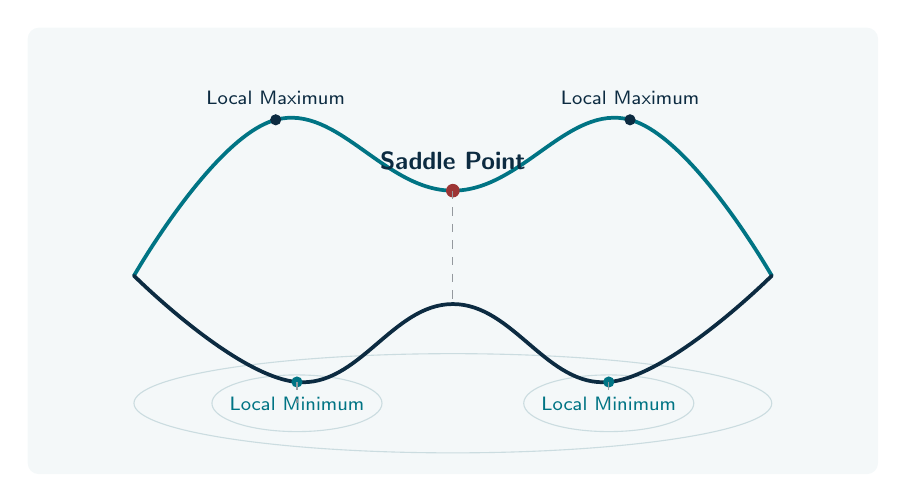
\begin{tikzpicture}[scale=0.9, baseline]
  % 3D Loss Landscape Contour & Surface representation
  \fill[boxbg,rounded corners=4pt] (-6,-2.8) rectangle (6,3.5);
  
  % Contour ellipses at bottom
  \draw[borderblue!80, line width=0.4pt] (0,-1.8) ellipse (4.5cm and 0.7cm);
  \draw[borderblue!80, line width=0.4pt] (-2.2,-1.8) ellipse (1.2cm and 0.4cm);
  \draw[borderblue!80, line width=0.4pt] (2.2,-1.8) ellipse (1.2cm and 0.4cm);
  
  % Surface mesh outline
  \draw[bookcurve, color=secondaryblue] plot [smooth, tension=0.7] coordinates {(-4.5,0) (-2.5,2.2) (0,1.2) (2.5,2.2) (4.5,0)};
  \draw[bookcurve, color=primaryblue] plot [smooth, tension=0.7] coordinates {(-4.5,0) (-2.2,-1.5) (0,-0.4) (2.2,-1.5) (4.5,0)};
  
  % Saddle Point and Max/Min points
  \filldraw[accentred] (0,1.2) circle (2.5pt) node[above=4pt, font=\sffamily\bfseries\small, color=primaryblue] {Saddle Point};
  \filldraw[primaryblue] (-2.5,2.2) circle (2pt) node[above=2pt, font=\sffamily\scriptsize] {Local Maximum};
  \filldraw[primaryblue] (2.5,2.2) circle (2pt) node[above=2pt, font=\sffamily\scriptsize] {Local Maximum};
  \filldraw[secondaryblue] (-2.2,-1.5) circle (2pt) node[below=2pt, font=\sffamily\scriptsize] {Local Minimum};
  \filldraw[secondaryblue] (2.2,-1.5) circle (2pt) node[below=2pt, font=\sffamily\scriptsize] {Local Minimum};

  % Projection lines
  \draw[dashed, warmgray!70] (0,1.2) -- (0,-0.4);
  \draw[dashed, warmgray!70] (-2.2,-1.5) -- (-2.2,-1.8);
  \draw[dashed, warmgray!70] (2.2,-1.5) -- (2.2,-1.8);
\end{tikzpicture}
\end{center}

\begin{itemize}
    \item To identify if you are at a saddle point versus a local minimum, you look at the spectrum of the Hessian. If the gradient is near zero, we use eigen-decomposition of the Hessian.
    \item If we find any negative eigenvalues, you are at a saddle point.
    \item The eigenvector corresponding to the most negative eigenvalue points in the direction of the steepest descent to escape the saddle point.
\end{itemize}

\subsection{Momentum}

Keep a velocity that accumulates past gradients:
\begin{align}
v_t &= \beta v_{t-1} + (1 - \beta) \frac{\partial L}{\partial w} \\
w_t &= w_{t-1} - \eta v_t
\end{align}
$\beta$ is typically $0.9$ (meaning velocity is 90\% memory, 10\% new gradient).

\begin{examplebox}[Momentum Calculation]
Given $\beta = 0.9$, $\eta = 0.1$, and $\frac{\partial L}{\partial w} = 2$:
\begin{align*}
v_1 &= 0.9 \times 0 + 0.1 \times 2 = 0.2, \quad &w_1 &= w_0 - 0.1 \times 0.2 = -0.02 \\
v_2 &= 0.9 \times 0.2 + 0.1 \times 2 = 0.38, \quad &w_2 &= w_1 - 0.1 \times 0.38 = -0.058
\end{align*}
\end{examplebox}

Notice: $v$ keeps growing when gradient keeps pointing the same way. This is what accelerates convergence along consistent directions, and cancels out in oscillating directions (because opposite-sign gradients average out).

\subsection{Nesterov Accelerated Gradient (NAG)}

A smarter variant; you compute the gradient not at the current $w$, but at the look-ahead position resulting from current velocity (at the position reached after applying current velocity). This corrects overshooting slightly earlier than classical momentum.

\begin{align}
w_{\text{lookahead}} &= w_{t-1} - \eta \beta v_{t-1} \\
v_t &= \beta v_{t-1} + (1 - \beta) \frac{\partial L}{\partial w_{\text{lookahead}}} \\
w_t &= w_{t-1} - \eta v_t
\end{align}

So NAG is a ``look-ahead'' version of momentum; it calculates the gradient at the predicted next position ($w_{t-1} - \eta \beta v_{t-1}$) rather than the current position, allowing for more responsive corrections.

\subsection{Adaptive Learning Rate Methods}

The core idea: give each parameter its own effective learning rate, based on how large its past gradients have been.

\subsubsection{Adagrad}

Accumulate the sum of squared gradients per parameter:
\begin{align}
G_t &= G_{t-1} + \left( \frac{\partial L}{\partial w} \right)^2 \\
w_t &= w_{t-1} - \frac{\eta}{\sqrt{G_t} + \varepsilon} \frac{\partial L}{\partial w}
\end{align}

\begin{itemize}
    \item Parameters that get large/frequent gradients $\to G$ grows $\to$ step shrinks.
    \item Parameters that get small/rare gradients $\to$ step stays large.
\end{itemize}

Adagrad adapts the learning rate based on the sum of squares of historical gradients. It performs well on sparse data (like word embeddings), but suffers from a vanishing learning rate because the denominator grows monotonically.

\subsubsection{RMSProp}

Solves Adagrad's decay issue by using an exponentially weighted moving average of squared gradients, allowing it to forget older, less relevant gradients:
\begin{align}
S_t &= \beta S_{t-1} + (1 - \beta) \left( \frac{\partial L}{\partial w} \right)^2 \\
w_t &= w_{t-1} - \frac{\eta}{\sqrt{S_t} + \varepsilon} \frac{\partial L}{\partial w}
\end{align}

Now old gradients fade out instead of accumulating forever, so the learning rate doesn't die. $\beta$ is typically $0.99$ or $0.999$.

\subsubsection{Adam (Adaptive Moment Estimation)}

Combines both Momentum (first moment) and RMSProp (second moment):
\begin{align}
m_t &= \beta_1 m_{t-1} + (1 - \beta_1) \frac{\partial L}{\partial w} \qquad (\text{mean of gradients}) \\
v_t &= \beta_2 v_{t-1} + (1 - \beta_2) \left( \frac{\partial L}{\partial w} \right)^2 \qquad (\text{second moment}) \\
\hat{m}_t &= \frac{m_t}{1 - \beta_1^t} \qquad (\text{bias correction}) \\
\hat{v}_t &= \frac{v_t}{1 - \beta_2^t} \qquad (\text{bias correction}) \\
w_t &= w_{t-1} - \frac{\eta \hat{m}_t}{\sqrt{\hat{v}_t} + \varepsilon}
\end{align}
\textbf{Default parameters:} $\beta_1 = 0.9$, $\beta_2 = 0.999$, $\varepsilon = 10^{-8}$.

\paragraph{Why bias correction?} $m$ and $v$ start at $0$, so early in training they are biased toward $0$. Dividing by $1 - \beta_1^t$ for $m_t$ and $1 - \beta_2^t$ for $v_t$ compensates. At $t=1$, with $\beta_2 = 0.999$, $1 - \beta_2^1 = 0.001$, so $\hat{v}_1 = v_1 / 0.001$---a large correction that shrinks as $t$ grows and the bias fades naturally.

Adam is the default choice for most deep learning today because it is robust to learning rate choice and works well out of the box on noisy, sparse, non-stationary problems.

\subsubsection{AdamW (Decoupled Weight Decay)}

Standard Adam applies weight decay ($L_2$ regularization) by adding $\lambda w$ to the gradient before the Adam math. But this means weight decay gets scaled by the adaptive learning rate too, which is not what you want (regularization strength shouldn't depend on gradient history).

AdamW decouples it:
\begin{equation}
w_t = w_{t-1} - \eta \left( \frac{\hat{m}_t}{\sqrt{\hat{v}_t} + \varepsilon} \right) - \eta \lambda w_{t-1}
\end{equation}

AdamW fixed this by applying weight decay directly to the weight (post update), ensuring that every weight is penalized proportionally to its magnitude, regardless of its historical gradient. This leads to significantly better generalization in deep neural networks and Transformers.

This is now the standard optimizer for training Transformers, LLMs, and most modern vision models (ViT, ResNet, etc.).

\subsection{Optimizer vs Schedule}

\begin{itemize}
    \item \textbf{Optimizer (e.g., AdamW):} Responsible for the weight update equations at each time step $t$. It decides how to move based on the gradient and momentum.
    \item \textbf{Schedule (Learning Rate Schedule):} Determines the magnitude of the step size (learning rate) that the optimizer takes at each step.
    \item \textbf{Interaction:} AdamW calculates velocity and gradient, while the scheduler controls step size. Without a scheduler, AdamW would take very large steps in the beginning because velocity is uncalibrated ($\hat{v} \approx 0$), leading to unstable gradient exploration.
\end{itemize}

\paragraph{Learning Rate Schedules:}
\begin{itemize}
    \item \textbf{Step Decay:} Reducing the learning rate by a factor (e.g., $\times 0.1$) every fixed number of epochs.
    \item \textbf{Cosine Annealing:} Making the learning rate follow a cosine curve to gradually decrease to near zero by the end of training (the most common).
    \item \textbf{Warmup:} Starting with a very small learning rate and increasing it gradually over initial steps. This is essential in Transformers because velocity is unstable in the beginning, and starting with a large learning rate can cause model collapse.
    \item \textbf{One-Cycle Policy:} Increasing the learning rate then decreasing it during training, while moving velocity inversely (high velocity when learning rate is low and vice versa).
\end{itemize}

\subsection{First-Order vs Second-Order Geometry}

\begin{itemize}
    \item \textbf{First-Order Methods (e.g., AdamW):} First-order methods use only the first derivative (gradient) to estimate the direction of the minimum.
    \item \textbf{Second-Order Methods (e.g., Shampoo, Newton, K-FAC):} Advanced optimizers using second-order methods do not stop at looking at gradient direction, but calculate curvature using second derivatives.
\end{itemize}

\subsection{Advanced Methods}

Methods attempting to understand loss function curvature for faster convergence, though computationally expensive:
\begin{itemize}
    \item \textbf{Newton's Method:} Uses the Hessian Matrix containing second derivatives of the loss function. Its complexity is $O(n^3)$, making it computationally infeasible for large models.
    \item \textbf{Natural Gradient Descent:} Uses the Fisher Information Matrix; more accurate but still expensive.
    \item \textbf{K-FAC:} Uses Kronecker-factored approximate curvature on second derivatives, enabling practical application in deep neural networks.
    \item \textbf{Shampoo:} Recent optimizer from Google. Acts as a second-order method by treating each layer independently to accelerate convergence.
    \item \textbf{LAMB:} Designed specifically for training large models with massive batch sizes by adapting the learning rate layer-wise.
    \item \textbf{Lion, Sophia, Adan (2023--2024 Optimizers):} Modern optimizers aimed at making LLM training more memory- and time-efficient using clever estimates of derivatives (e.g., diagonal Hessian in Sophia, sign operation in Lion).
\end{itemize}

\paragraph{Advanced Methods Summary (Shampoo / Second-Order):} Future research directions attempting to find shortcut paths by understanding landscape curvature (Hessian) instead of relying solely on the refined gradient estimates that AdamW uses.

% !TEX root = ../main.tex
\chapter{Convolutional Neural Networks (CNN)}

\section{What Is a Convolutional Neural Network?}

A Convolutional Neural Network (CNN) is a type of neural network designed to process images by using small kernels (or filters) that slide across the image. Instead of learning separate weights for every input-output connection, the CNN learns only the kernel's weights and reuses them at every position in the image.

As the kernel moves across the image, it computes an output value at each location. Collecting all these outputs produces a \textbf{feature map}, which shows how strongly the learned pattern (such as an edge or corner) appears at every location in the image.

\section{The Problem with Traditional Fully Connected Neural Networks}

When images are processed using a traditional fully connected neural network (MLP), the image must first be flattened into a one-dimensional vector. This creates two major problems: a very large number of parameters and the loss of the image's spatial structure.

For example, connecting a $28 \times 28$ image (784 pixels) to a layer of 128 neurons requires:

\[
784 \times 128 = 100,352 \text{ weights}
\]

Moreover, the network treats each pixel independently, without explicitly considering the spatial relationships between neighboring pixels.

\section{The CNN Solution}

A Convolutional Neural Network (CNN) addresses these limitations through \textbf{local connectivity} and \textbf{parameter sharing}. Rather than connecting every input pixel to every neuron, it uses a small number of learnable parameters to extract local patterns from the image.

For example, a $3 \times 3$ kernel contains only 9 weights (ignoring the bias), compared with the 100,352 weights required by the MLP example above. These parameters are reused across different image locations, significantly reducing the number of learnable parameters.

\begin{itemize}
    \item \textbf{MLP:} 784 inputs $\rightarrow$ 100,352 weights, with each input connected to all 128 neurons.
    \item \textbf{CNN:} One $3 \times 3$ kernel $\rightarrow$ 9 weights (ignoring the bias), reused across the image to detect the same pattern at different locations.
\end{itemize}


\clearpage
\begin{figure}[htbp]
    \centering
    \includegraphics[width=0.92\textwidth]{2-saddle point - CNN/photo_5_2026-07-28_02-59-38.jpg}
    \caption{CNN Structure Overview showing feature extraction layers and MLP classification head.}
    \label{fig:cnn_structure}
\end{figure}

\clearpage
\section{Convolution Operation}

An RGB image is composed of three channels: red, green, blue. Each channel containing intensity values of one color. During Convolution, a kernel passes across all three channels simultaneously. The filter has the same depth as the input.

\begin{center}
\begin{minipage}{0.45\textwidth}
\centering
\textbf{Input Image ($5 \times 5$)} \\[0.4em]
\begin{tabular}{|c|c|c|c|c|}
\hline
12 & 255 & 128 & 12 & 13 \\ \hline
1 & 11 & 12 & 14 & 15 \\ \hline
115 & 30 & 40 & 16 & 17 \\ \hline
18 & 19 & 20 & 21 & 22 \\ \hline
23 & 24 & 25 & 26 & 27 \\ \hline
\end{tabular}
\end{minipage}
\quad $\mathbf{\times}$ \quad
\begin{minipage}{0.35\textwidth}
\centering
\textbf{Kernel ($3 \times 3$)} \\[0.4em]
\begin{tabular}{|c|c|c|}
\hline
-1 & -1 & -1 \\ \hline
0 & 0 & 0 \\ \hline
1 & 1 & 1 \\ \hline
\end{tabular}
\end{minipage}
\end{center}

Computes a weighted sum of local pixel values:
\begin{equation}
32 \times 32 \times 3 \xrightarrow{\text{Conv } 3 \times 3 \times 3} 30 \times 30 \times 1
\end{equation}

Repeating this process across the entire image creates a feature map that highlights specific patterns.

\section{Kernel (Filter)}

A kernel is a small matrix of learnable weights responsible for extracting features from an image, such as edges, corners, and textures. It slides across the image, performing element-wise multiplication with local pixel values and summing the results to produce a feature map. Its weights are initially assigned random values and gradually updated during training through backpropagation and gradient descent to learn useful visual features.

\section{Output Dimension \& Zero Padding}

The output size after a Convolution depends on four things:
\begin{itemize}
    \item Input size ($N$)
    \item Kernel size ($K$)
    \item Stride ($S$)
    \item Padding ($P$)
\end{itemize}

\begin{equation}
\text{Output Size} = \left\lfloor \frac{N - K + 2P}{S} \right\rfloor + 1
\end{equation}

\begin{equation}
\text{Example: } \left( \frac{32 - 3 + 2(0)}{1} \right) + 1 = 30 \quad (30 \times 30)
\end{equation}

\paragraph{Convolution: Zero Padding}
\begin{itemize}
    \item \textbf{Problem:} The output is smaller than the input. If the input is $28 \times 28$ and the filter is $3 \times 3$, you can have at most 13 convolutional layers (the output of the 13th layer is $2 \times 2$).
    \item \textbf{Solution (Zero Padding):} Adds a border of zeros around the input image before applying the convolution. This preserves more edge information and can keep the output size the same as the input (for example, using a $3 \times 3$ kernel with padding 1 and stride 1).
\end{itemize}

\section{Stride}

\begin{itemize}
    \item \textbf{Stride = 1:} The kernel moves 1 step each time.
    \item \textbf{Stride = 2:} The kernel moves 2 steps each time.
\end{itemize}

Using a Stride of 1 makes the kernel move one pixel at a time, producing large feature maps and increasing computation and memory usage. A large Stride moves the kernel more than one pixel at once, reducing the size of the output feature map. This decreases computation and memory requirements while preserving the most important features.

\begin{figure}[htbp]
\centering
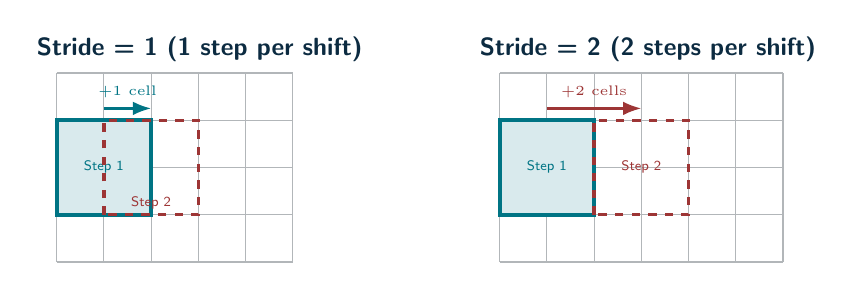
\begin{tikzpicture}[scale=0.75]
  % Stride = 1 Illustration
  \begin{scope}[shift={(0,0)}]
    \node[anchor=west, font=\sffamily\bfseries\small, color=primaryblue] at (-0.5, 3.6) {Stride = 1 (1 step per shift)};
    \draw[step=0.8cm, warmgray!50, thin] (0,0) grid (4,3.2);
    % Step 1 box
    \draw[line width=1.4pt, secondaryblue, fill=secondaryblue!15] (0, 0.8) rectangle (1.6, 2.4);
    \node[font=\sffamily\tiny, secondaryblue] at (0.8, 1.6) {Step 1};
    % Step 2 box (shifted by 1)
    \draw[line width=1.2pt, accentred, dashed] (0.8, 0.8) rectangle (2.4, 2.4);
    \node[font=\sffamily\tiny, accentred] at (1.6, 1.0) {Step 2};
    \draw[-{Latex}, secondaryblue, thick] (0.8, 2.6) -- (1.6, 2.6) node[midway, above, font=\tiny] {+1 cell};
  \end{scope}

  % Stride = 2 Illustration
  \begin{scope}[shift={(7.5,0)}]
    \node[anchor=west, font=\sffamily\bfseries\small, color=primaryblue] at (-0.5, 3.6) {Stride = 2 (2 steps per shift)};
    \draw[step=0.8cm, warmgray!50, thin] (0,0) grid (4.8,3.2);
    % Step 1 box
    \draw[line width=1.4pt, secondaryblue, fill=secondaryblue!15] (0, 0.8) rectangle (1.6, 2.4);
    \node[font=\sffamily\tiny, secondaryblue] at (0.8, 1.6) {Step 1};
    % Step 2 box (shifted by 2)
    \draw[line width=1.2pt, accentred, dashed] (1.6, 0.8) rectangle (3.2, 2.4);
    \node[font=\sffamily\tiny, accentred] at (2.4, 1.6) {Step 2};
    \draw[-{Latex}, accentred, thick] (0.8, 2.6) -- (2.4, 2.6) node[midway, above, font=\tiny] {+2 cells};
  \end{scope}
\end{tikzpicture}
\caption{Visual illustration of Stride operation mechanism across feature grids.}
\label{fig:stride_diagram}
\end{figure}

\section{Pooling}

Pooling is a downsampling operation that reduces the spatial dimension (height and width) of a feature map while retaining its most important information. It helps reduce computation, memory usage, and the risk of overfitting.
\begin{figure}[H]
\centering
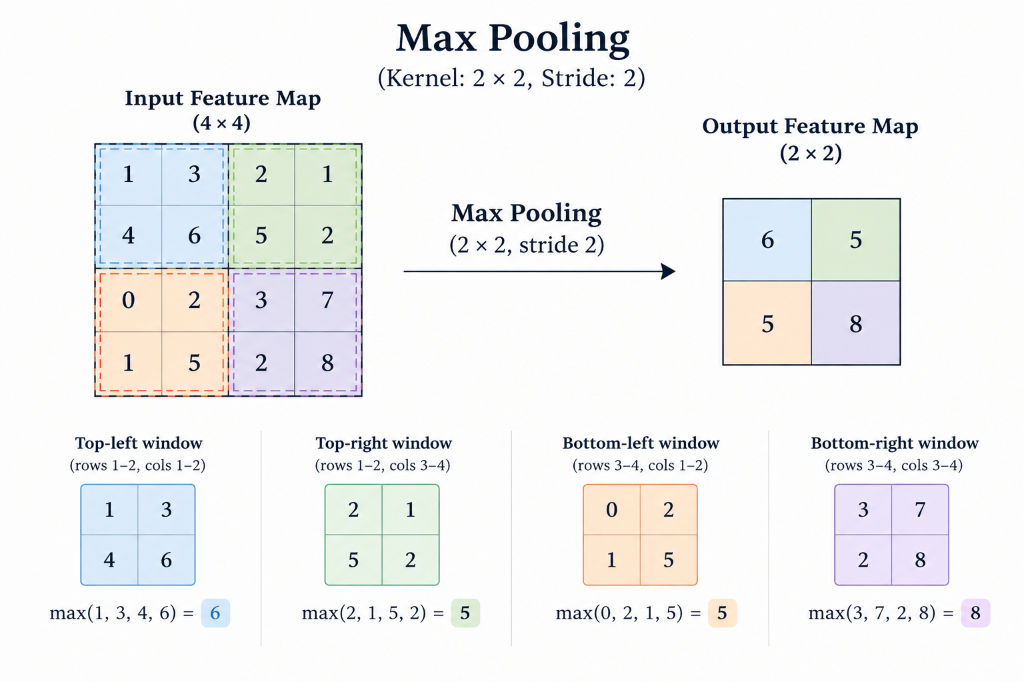
\includegraphics[width=0.95\textwidth]{figures/max_pooling.png}
\end{figure}
\begin{advbox}[Types of Pooling]
\begin{enumerate}[leftmargin=1.5em]
    \item \textbf{Max Pooling:} Selects the maximum value from each pooling window. It is the most commonly used pooling operation because it preserves the strongest features.
    \item \textbf{Average Pooling:} Computes the average value of each pooling window, producing a smoother feature map.
\end{enumerate}

\tcbline

\textbf{Note:} Pooling does not change the number of channels; it only reduces the height and width of the feature maps.

\textbf{Overlap Pooling (Stride = $2 \times 2$):} The windows touch each other but do not share any element (non-overlapping). If Stride = 1, the windows share many elements (overlapping).
\end{advbox}

\paragraph{Activation Function (Adding Non-Linearity)}

\begin{center}
\begin{minipage}{0.4\textwidth}
\centering
\textbf{Input Feature Map} \\[0.4em]
\begin{tabular}{|c|c|c|c|}
\hline
15 & 20 & 13 & -5 \\ \hline
250 & 15 & -4 & -3 \\ \hline
12 & 11 & 10 & 7 \\ \hline
-20 & 5 & -7 & 150 \\ \hline
\end{tabular}
\end{minipage}
\quad $\xrightarrow{\text{\textbf{ReLU}}}$ \quad
\begin{minipage}{0.4\textwidth}
\centering
\textbf{Activated Output} \\[0.4em]
\begin{tabular}{|c|c|c|c|}
\hline
15 & 20 & 13 & 0 \\ \hline
250 & 15 & 0 & 0 \\ \hline
12 & 11 & 10 & 7 \\ \hline
0 & 5 & 0 & 150 \\ \hline
\end{tabular}
\end{minipage}
\end{center}

\section{CNN Step-by-Step Pipeline}

\begin{propertybox}[Step-by-Step CNN Execution Flow]
\textbf{Input:} $28 \times 28 \times 3$
\begin{itemize}
    \item \textbf{Conv Layer 1:} 8 Kernels ($3 \times 3 \times 3$). Each kernel scans across all 3 channels simultaneously, summing them into one value per position $\to$ 8 Kernels = 8 output feature maps. \quad $\mathbf{\to \text{Output: } 26 \times 26 \times 8}$
    \item \textbf{Activation (ReLU):} Applied element-wise to all 8 feature maps.
    \item \textbf{Pooling (Max Pool $2 \times 2$):} $26 \times 26 \times 8 \to 13 \times 13 \times 8$
    \item \textbf{Conv Layer 2:} 16 Kernels ($3 \times 3 \times 8$) $\mathbf{\to \text{Output: } 11 \times 11 \times 16}$
    \item \textbf{Repeat Conv + Pool block}
    \item \textbf{Flatten $\to$ Linear (MLP) $\to$ Final Classification}
\end{itemize}
\end{propertybox}

\section{Backpropagation \& Parameter Gradients in CNNs}

Unlike traditional image processing filters such as Sobel or Gaussian chosen manually, CNNs treat the values within each kernel as learnable parameters. Kernel weights are set to small random values. Through the training process, these weights are iteratively updated using Gradient Descent following the backpropagation rule:

\begin{equation}
w_{m,n}^{(t+1)} = w_{m,n}^{(t)} - \eta \frac{\partial L}{\partial w_{m,n}}
\end{equation}

\paragraph{Gradient w.r.t. Kernel $w$:}
\begin{equation}
\frac{\partial L}{\partial w_{m,n}} = \sum_{i,j} \frac{\partial L}{\partial Y_{i,j}} \cdot \frac{\partial Y_{i,j}}{\partial w_{m,n}}, \qquad \text{where } \frac{\partial Y_{i,j}}{\partial w_{m,n}} = X_{i+m, j+n}
\end{equation}

\begin{equation}
\boxed{\frac{\partial L}{\partial w_{m,n}} = \sum_{i,j} dY_{i,j} \cdot X_{i+m, j+n}}
\end{equation}

\paragraph{Gradient w.r.t. Bias $b$:}
\begin{equation}
\frac{\partial L}{\partial b} = \sum_{i,j} dY_{i,j}
\end{equation}

\paragraph{Gradient w.r.t. Input $X$:}
\begin{equation}
\frac{\partial L}{\partial X_{p,q}} = \sum_{m,n} dY_{p-m, q-n} \cdot w_{m,n}
\end{equation}

\begin{center}
\textbf{Forward:} $X \xrightarrow{\quad \text{Conv} \quad} Y \qquad \mathbf{\vert} \qquad \textbf{Backward:} dY \xrightarrow{\quad dW, dX \quad} dX$
\end{center}

\section{Batch Normalization}

\begin{itemize}
    \item \textbf{Problem:} Feature scaling was applied only once, to the raw input $x$. But every hidden layer's output $z^{(k)}$ is also a feature vector whose scale drifts during training, causing the same slow-convergence problem as before.
    \item \textbf{Solution:} Standardize the output of every hidden layer at every training step — not just the input once.
\end{itemize}

\subsection{The Memory Problem \& Channel-Wise Solution}

Naively, Batch Normalization needs one $\mu$ (mean), $\sigma$ (standard deviation), $\gamma$, $\beta$ per pixel position. For a $150 \times 150 \times 64$ feature map, that requires:
\begin{equation}
4 \times 150 \times 150 \times 64 = 5.76\text{M parameters for one Batch Normalization layer}
\end{equation}

\textbf{Solution:} Share one scalar per channel instead of per pixel position. Make it $1 \times 1 \times 64$ instead of $150 \times 150 \times 64$. All spatial positions in a channel $R$ reuse the same $\gamma, \beta, \mu, \sigma$, reducing the count to:
\begin{equation}
4 \times 64 = \boxed{256 \text{ parameters}}
\end{equation}
\subsection{Keras Implementation}

\begin{verbatim}
model = models.Sequential()
model.add(layers.Conv2D(10, (5, 5), input_shape=(28, 28, 1)))
model.add(layers.BatchNormalization())
model.add(layers.Activation('relu'))
model.add(layers.MaxPooling2D((2, 2)))

model.add(layers.Conv2D(20, (5, 5)))
model.add(layers.BatchNormalization())
model.add(layers.Activation('relu'))
model.add(layers.MaxPooling2D((2, 2)))

model.add(layers.Flatten())
model.add(layers.Dense(10, activation='softmax'))
\end{verbatim}

\begin{table}[htbp]
\centering
\caption{Parameter Count Before and After Adding Batch Normalization}
\label{tab}
\begin{tabular}{lcc}
\toprule
\textbf{Layer} & \textbf{Without BN} & \textbf{With BN} \\
\midrule
Conv2D\_1 & 260 & 260 \\
Batch Normalization\_1 & -- & 40 \\
Conv2D\_2 & 5,020 & 5,020 \\
Batch Normalization\_2 & -- & 80 \\
Dense & 3,210 & 3,210 \\
\midrule
\textbf{Total Parameters} & \textbf{8,490} & \textbf{8,610} \\
\textbf{Additional Parameters} & -- & \textbf{120} \\
\bottomrule
\end{tabular}
\end{table}

The version with BN converges roughly $10\times$ faster, reaching $\sim 98\%$ accuracy in 3 epochs instead of $\sim 30$. The extra parameters ($0.2\text{ MB}$ difference, negligible) buy a massive gain in convergence speed and training stability.

\section{Common CNN Architectures}

\subsection{LeNet-5 (1998)}

LeNet-5, proposed by Yann LeCun, Léon Bottou, Yoshua Bengio, and Patrick Haffner in 1998, is one of the earliest and most influential Convolutional Neural Networks (CNNs). It was designed for handwritten digit recognition and achieved remarkable performance on the MNIST dataset, demonstrating the effectiveness of convolutional neural networks for image classification.

The architecture consists of a sequence of convolutional, subsampling (average pooling), and fully connected layers:

\begin{itemize}
    \item \textbf{Input Layer:} A grayscale image of size $32 \times 32$.
    
    \item \textbf{Convolution Layers:} Convolution operations using $5 \times 5$ kernels extract local features such as edges and simple patterns. The first convolution layer produces 6 feature maps, while the second produces 16 feature maps.

    \item \textbf{Subsampling Layers:} Average pooling with a $2 \times 2$ window reduces the spatial dimensions of the feature maps, decreases computational cost, and provides a degree of translation invariance.

    \item \textbf{Fully Connected Layers:} The extracted features are flattened and passed through fully connected layers that combine the learned representations.

    \item \textbf{Output Layer:} A final fully connected layer produces probabilities for the ten digit classes (0--9).
\end{itemize}

LeNet-5 introduced several fundamental concepts that became standard in modern deep learning, including local receptive fields, shared convolutional weights, pooling operations, and end-to-end learning through backpropagation. Although relatively small compared with modern CNNs, it established the foundation for many successful convolutional network architectures developed in later years.
\begin{figure}[H]
\centering
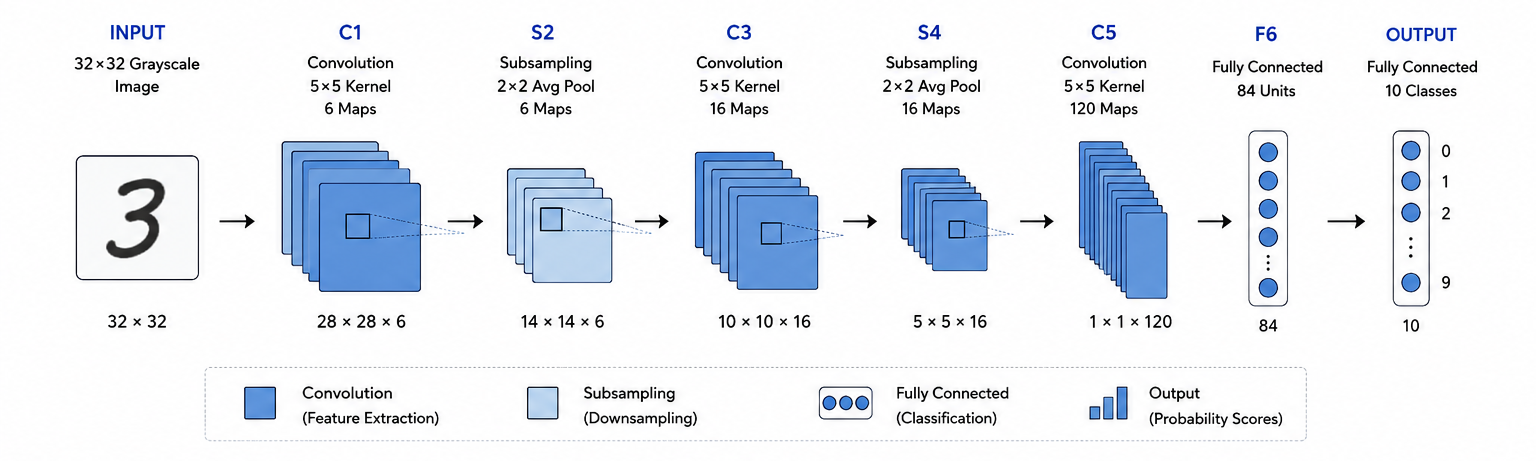
\includegraphics[width=0.95\textwidth]{figures/lenet1.png}
\end{figure}
\begin{figure}[H]
\centering
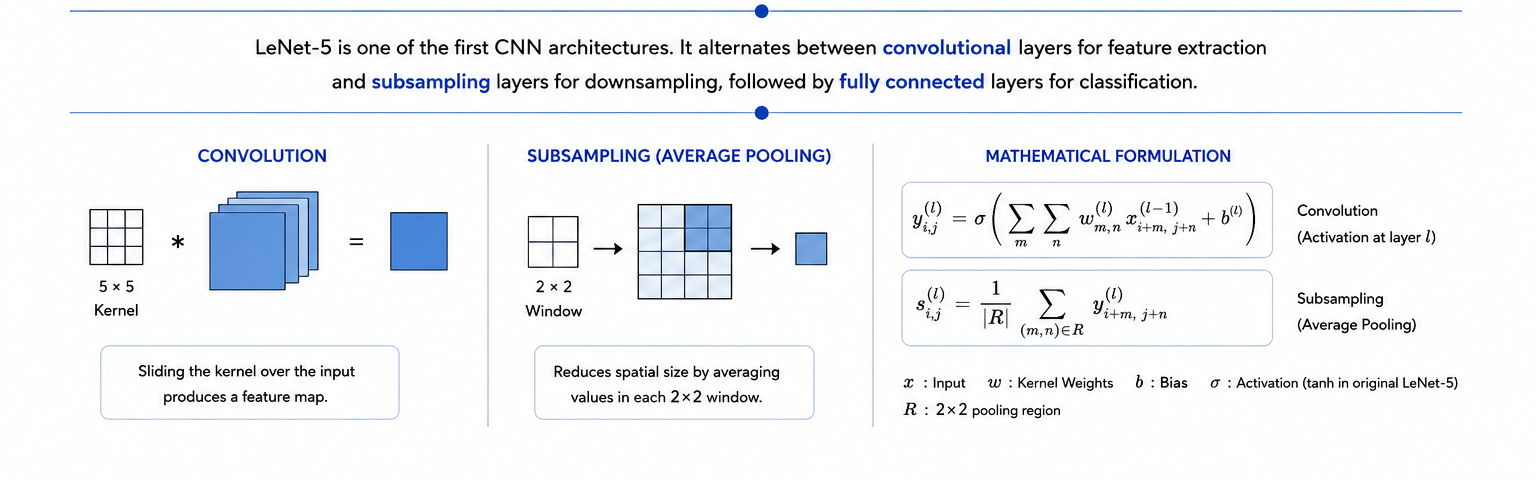
\includegraphics[width=0.95\textwidth]{figures/lenet2.png}
\end{figure}
\subsection{AlexNet (2012)}
5 Conv layers, 3 FC layers, 60M parameters. Key innovations:
\begin{enumerate}
    \item \textbf{ReLU instead of Sigmoid / Tanh:} Avoids the vanishing gradient problem.
    \item \textbf{Dropout in FC layers:} Acts as a regularizer to fight overfitting.
    \item \textbf{GPU Training:} Trained 1.2M images on GPUs instead of CPUs.
    \item \textbf{Large Stride and Kernels early ($11 \times 11$, Stride 4):} Aggressively downsamples big $224 \times 224$ inputs quickly, followed by smaller kernels ($5 \times 5, 3 \times 3$) deeper in.
\end{enumerate}
\begin{figure}[H]
\centering
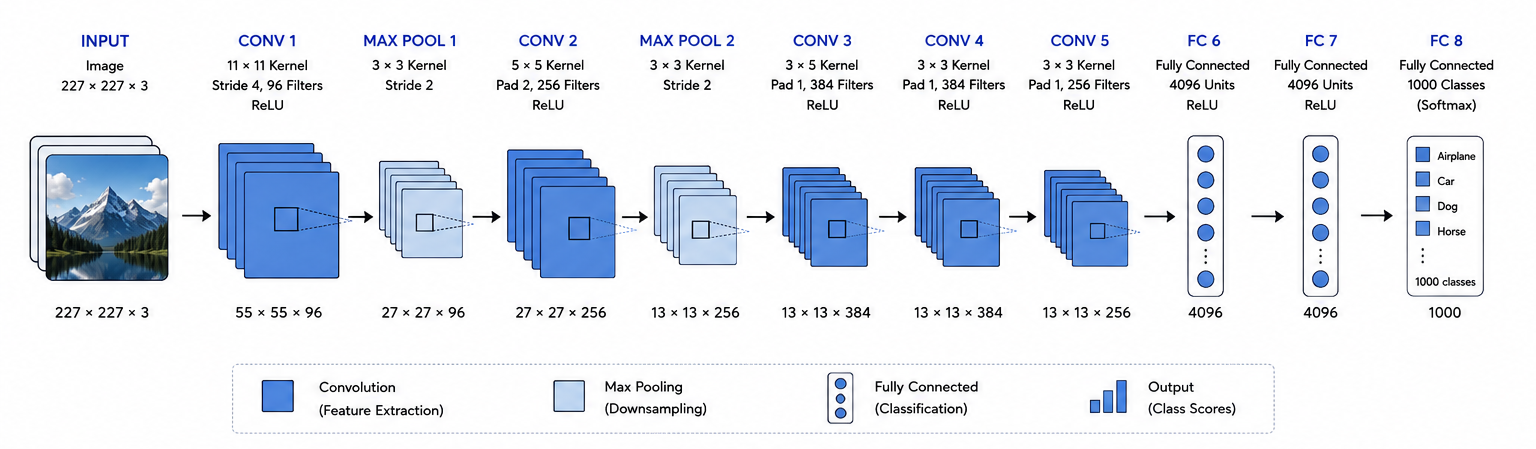
\includegraphics[width=0.95\textwidth]{figures/alexnet1.png}
\end{figure}
\begin{figure}[H]
\centering
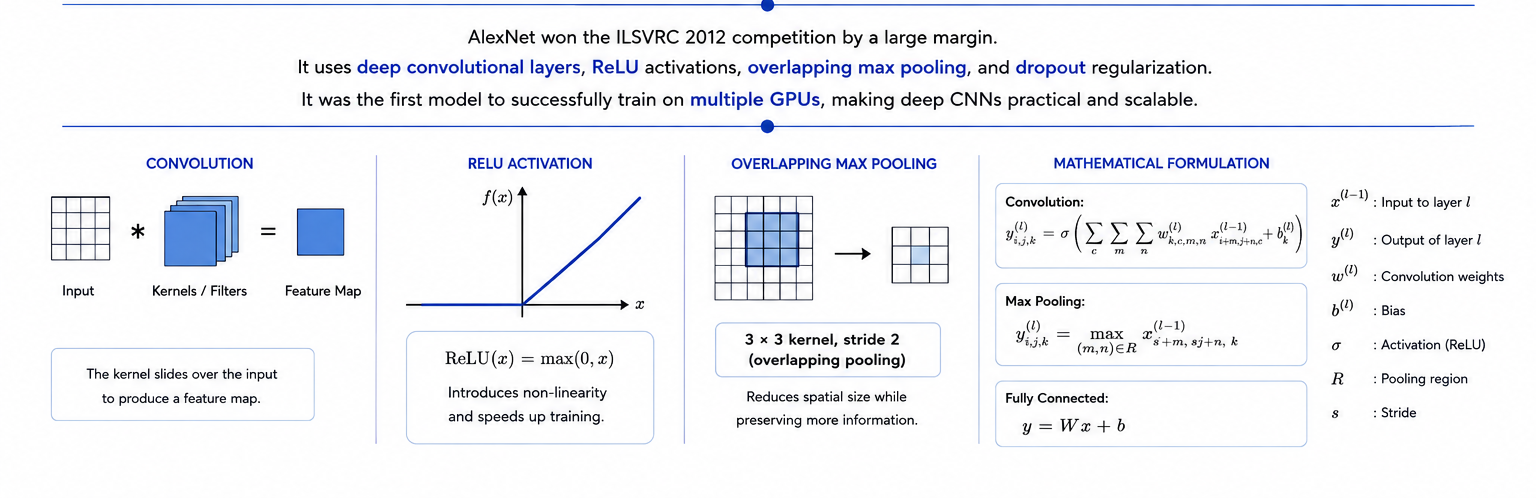
\includegraphics[width=0.95\textwidth]{figures/alexnet2.png}
\end{figure}
\begin{propertybox}[Historical Significance]
This is the paper that revived neural networks after the ``neural networks are dead'' period — winning ImageNet 2012 by a huge margin over traditional SIFT/HOG-based methods.
\end{propertybox}

\begin{center}
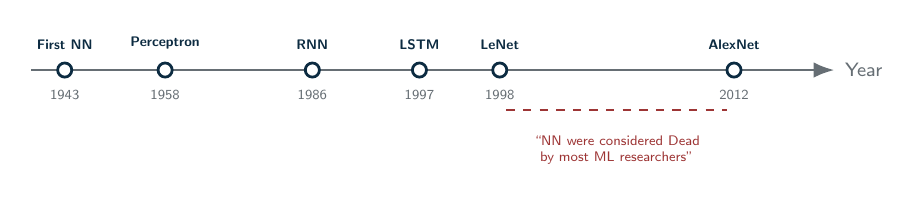
\begin{tikzpicture}[scale=0.85]
  \draw[-{Latex}, warmgray, line width=1pt] (0,0) -- (12,0) node[right, font=\sffamily\scriptsize] {Year};
  
  \foreach \x/\year/\label in {0.5/1943/First NN, 2.0/1958/Perceptron, 4.2/1986/RNN, 5.8/1997/LSTM, 7.0/1998/LeNet, 10.5/2012/AlexNet} {
    \draw[primaryblue, fill=white, line width=1pt] (\x,0) circle (3pt);
    \node[above=4pt, font=\sffamily\tiny\bfseries, color=primaryblue] at (\x,0) {\label};
    \node[below=4pt, font=\sffamily\tiny, color=warmgray] at (\x,0) {\year};
  }
  
  \draw[accentred, dashed, line width=0.8pt] (7.1,-0.6) -- (10.4,-0.6);
  \node[below=8pt, font=\sffamily\tiny, color=accentred, align=center] at (8.75,-0.5) {``NN were considered Dead\\by most ML researchers''};
\end{tikzpicture}
\end{center}

\subsection{VGG-16 (2014)}

VGG-16, proposed by Karen Simonyan and Andrew Zisserman in 2014, is a deep Convolutional Neural Network (CNN) known for its simple and uniform architecture. It uses only $3 \times 3$ convolution filters and consists of 13 convolutional layers followed by 3 fully connected layers (16 weight layers in total), with approximately 138 million trainable parameters. Despite its high computational cost, VGG-16 achieved excellent performance on ImageNet and became a widely used backbone for image classification, object detection, semantic segmentation, and transfer learning.

\begin{itemize}
    \item \textbf{Uniformity and depth via small kernels:} Instead of AlexNet's mix of large and small kernels, VGG uses only $3 \times 3$ convolutions stacked repeatedly before each pooling step, providing fewer parameters and extra non-linearity.
    \item \textbf{Fine-Tuning pattern still used today:} Freeze early conv blocks (1 to 4, generic features), fine-tune only the last conv block + custom FC head for a new task.
\end{itemize}
\begin{figure}[H]
\centering
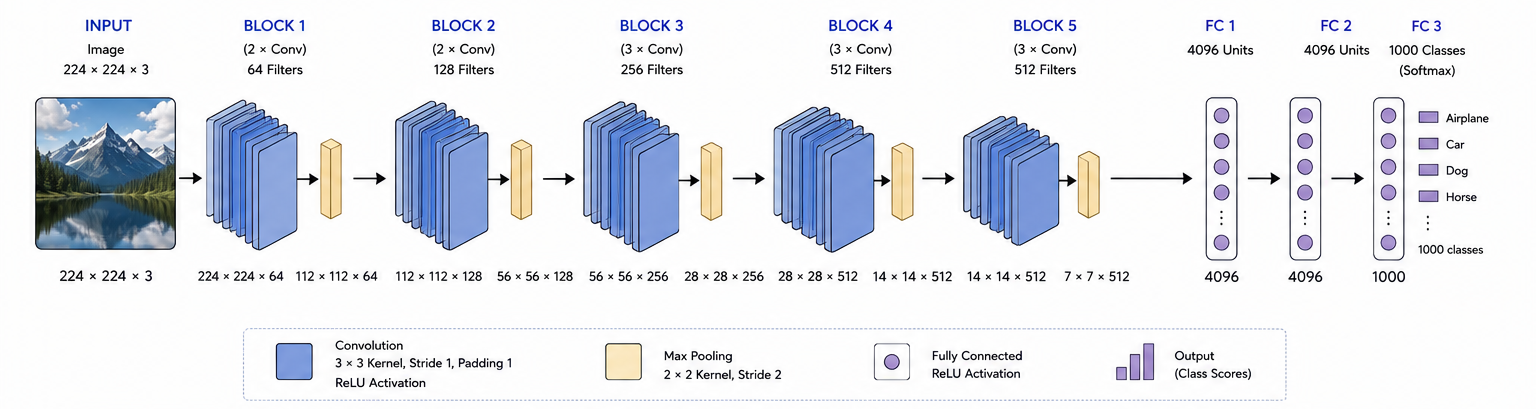
\includegraphics[width=0.95\textwidth]{figures/vgg1.png}
\end{figure}
\begin{figure}[H]
\centering
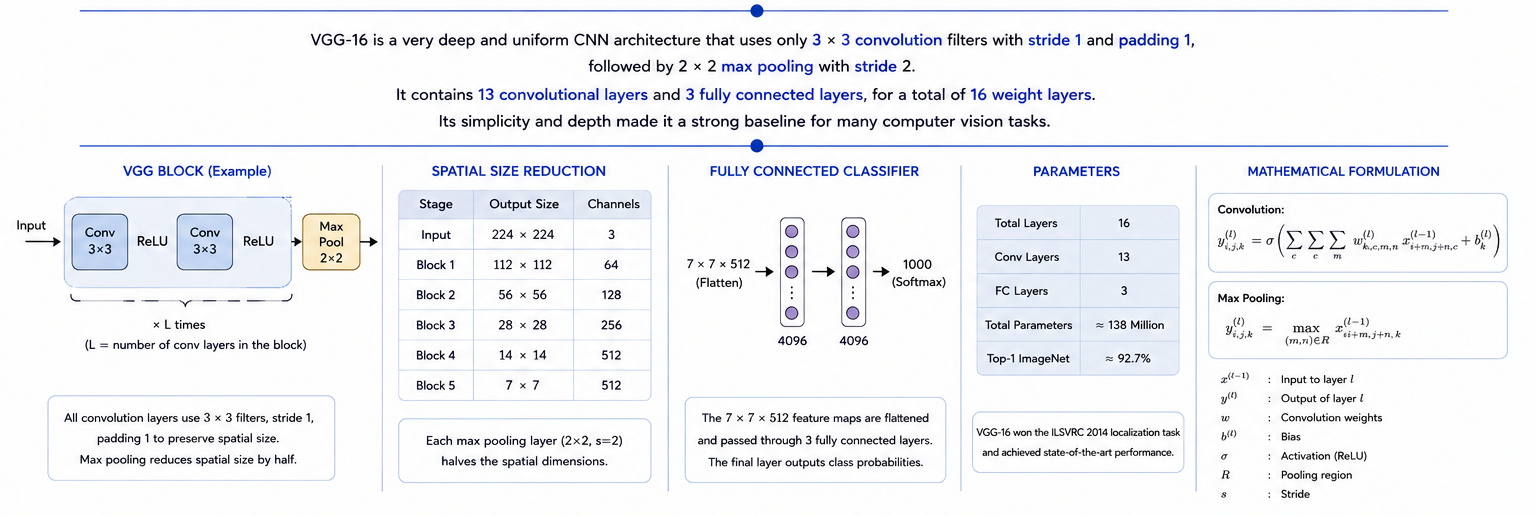
\includegraphics[width=0.95\textwidth]{figures/vgg2.png}
\end{figure}
\paragraph{Why Not Just Keep Stacking VGG-Style?}
Pushing plain sequential architectures past $\sim 20$ layers made both training and test error worse — not due to overfitting, but due to \textbf{vanishing gradients}.

\subsection{GoogLeNet / Inception (2014 / 2015)}
21 Conv layers + 1 FC layer, 5M parameters.
\begin{enumerate}
    \item \textbf{Inception Module:} Runs $1 \times 1$, $3 \times 3$, $5 \times 5$ convolutions and $3 \times 3$ max-pooling in parallel, then concatenates their outputs. The $1 \times 1$ convolution reduces dimensions before the $3 \times 3$ and $5 \times 5$ branches, keeping the model efficient (5M params vs VGG-16's 138M).
    \item \textbf{Auxiliary Outputs:} Extra Softmax classifiers added to intermediate layers during training only to provide direct gradients to earlier layers. Removed during inference.
    \item \textbf{Global Average Pooling instead of Flatten:} Replaces large Flatten + FC layers with Global Average Pooling, reducing feature maps to $1 \times 1 \times 1024$ before the final FC (1000) layer.
\end{enumerate}

\subsection{ResNet (2015)}
Up to 151 Conv layers + 1 FC layer. Introduces \textbf{Skip (residual) connections}:
\begin{equation}
y = F(x) + x
\end{equation}

Instead of learning the full mapping, the network learns the residual $F(x)$ and adds the original input $x$.
\begin{figure}[H]
\centering
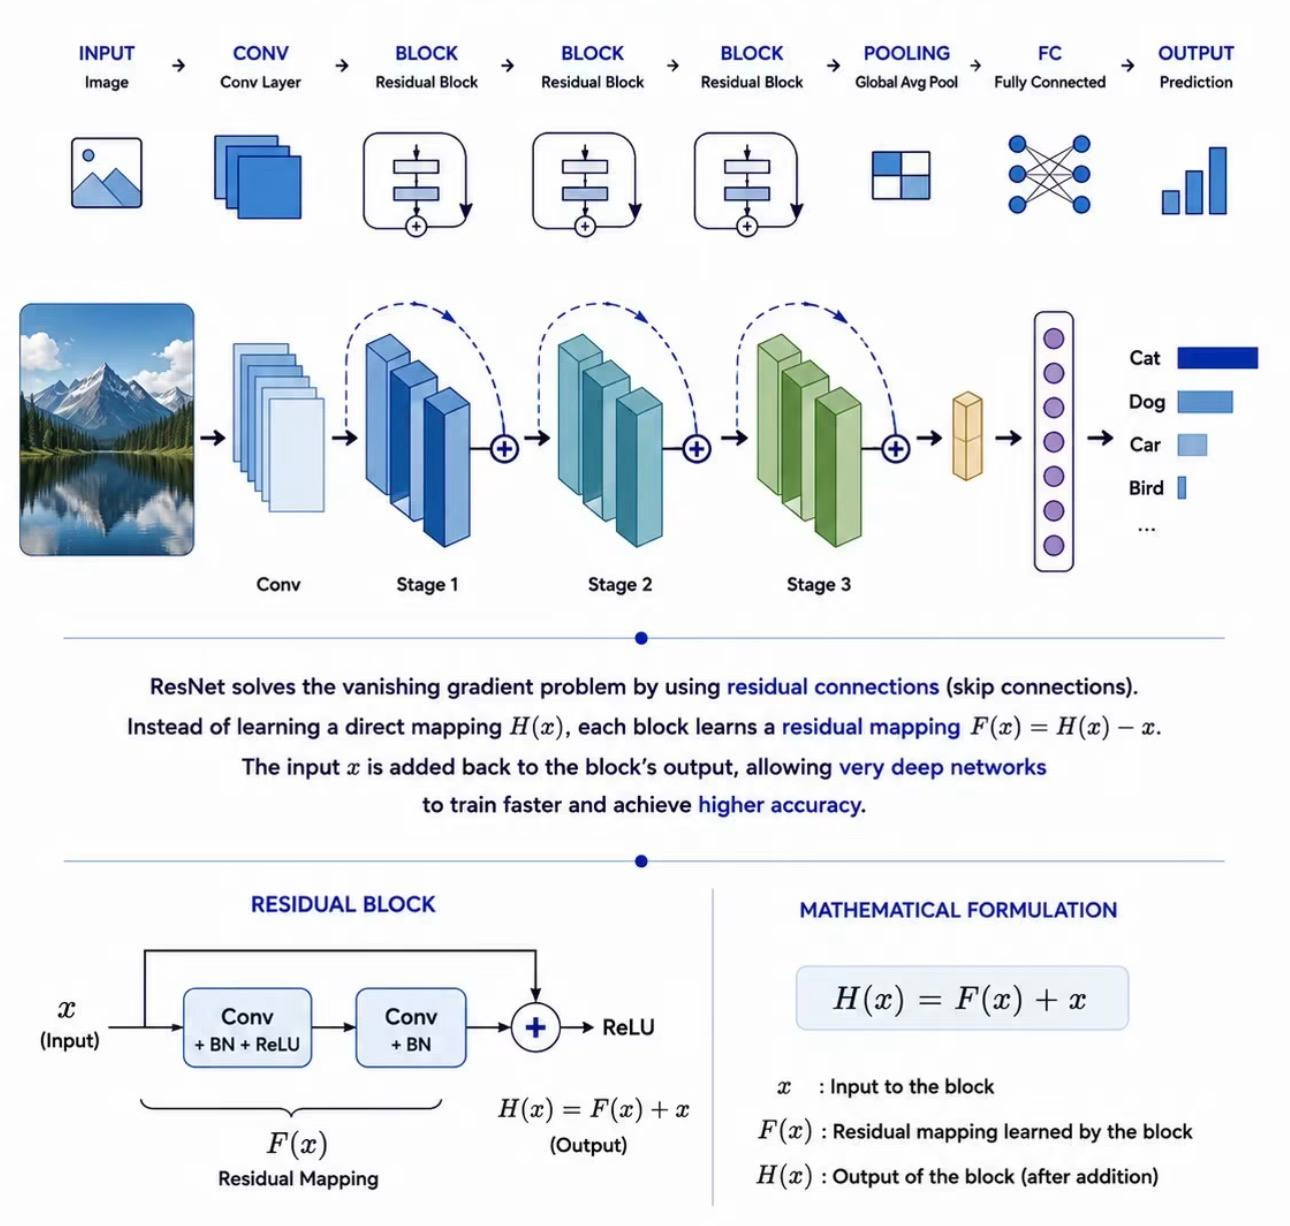
\includegraphics[width=0.95\textwidth]{figures/resnet.jpg}
\end{figure}
\paragraph{Why It Solved Vanishing Gradients:}
The identity connection $+x$ creates a direct gradient path:
\begin{equation}
\frac{\partial y}{\partial x} = \frac{\partial F(x)}{\partial x} + I
\end{equation}

The $I$ (identity) term acts as a gradient ``highway'', allowing gradients to flow even if $\frac{\partial F(x)}{\partial x}$ becomes very small. ResNet successfully trained 152 layers ($\sim 7\times$ deeper than VGG16), proving that deeper performance drops were optimization issues rather than limits of Deep Learning.

\subsection{U-Net (2015)}

U-Net is a convolutional neural network introduced by Olaf Ronneberger, Philipp Fischer, and Thomas Brox in 2015 for biomedical image segmentation. It follows an encoder--decoder architecture with symmetric skip connections, allowing the network to capture both high-level semantic information and fine spatial details.

The architecture consists of four main components:

\begin{itemize}
    \item \textbf{Encoder (Contracting Path):} Repeated applications of two $3\times3$ convolutions followed by ReLU activation and a $2\times2$ max pooling operation. The spatial resolution decreases while the number of feature channels increases.

    \item \textbf{Bottleneck:} The deepest part of the network, where feature maps contain the highest-level semantic information before reconstruction begins.

    \item \textbf{Decoder (Expanding Path):} Each stage performs upsampling using transposed convolution (or up-convolution), concatenates the corresponding encoder feature maps through skip connections, and applies two $3\times3$ convolutions with ReLU activation.

    \item \textbf{Output Layer:} A final $1\times1$ convolution maps the extracted features to the desired number of segmentation classes, producing a pixel-wise prediction.
\end{itemize}

The skip connections preserve high-resolution information lost during downsampling, enabling accurate localization while maintaining rich contextual information. This design makes U-Net highly effective for semantic segmentation tasks, especially when training data is limited.
\begin{figure}[H]
\centering
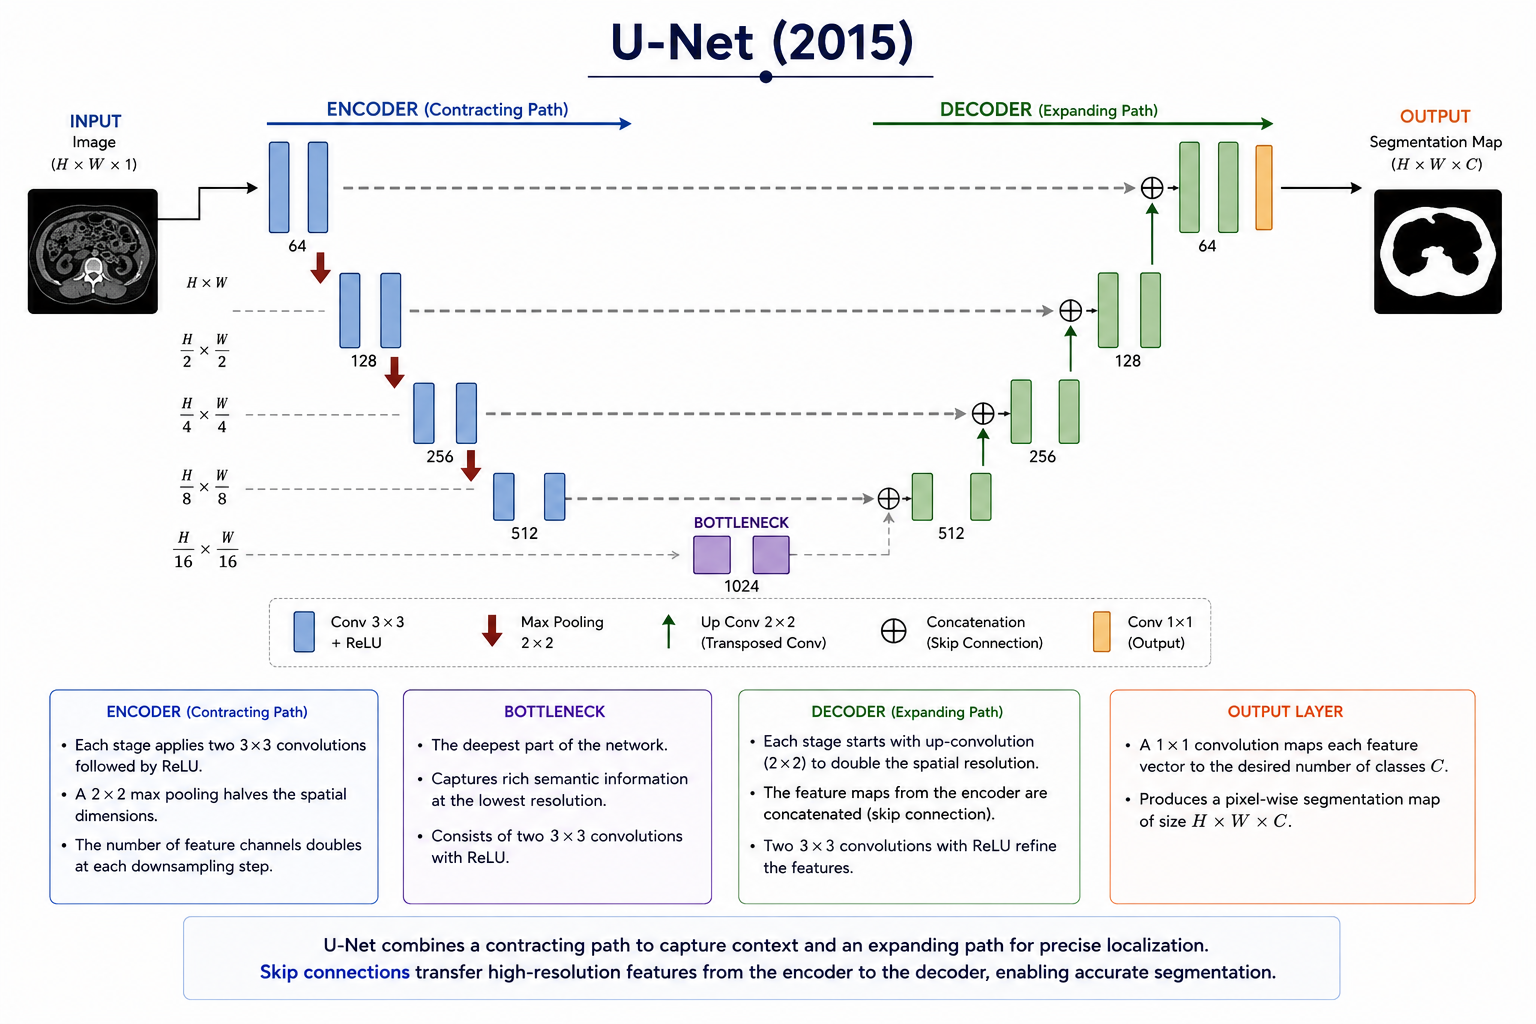
\includegraphics[width=0.95\textwidth]{figures/unet.png}
\end{figure}
\subsection{MobileNet (2017)}
Key Innovation ($\sim 4\text{M}$ parameters), designed specifically for mobile and edge devices.
\begin{enumerate}
    \item \textbf{Depthwise Separable Convolution:} Splits standard convolution into two steps:
    \begin{itemize}
        \item \textbf{Depthwise Convolution:} Applies one filter to each input channel separately.
        \item \textbf{Pointwise ($1 \times 1$) Convolution:} Combines information across channels.
    \end{itemize}
    \item \textbf{Global Average Pooling instead of Flatten:} Significantly reduces parameter count.
\end{enumerate}

MobileNet addressed the edge deployment problem by making CNNs small and efficient enough to run directly on smartphones and edge devices, reducing cloud reliance and improving latency, privacy, and memory efficiency.
 \begin{figure}[H]
\centering
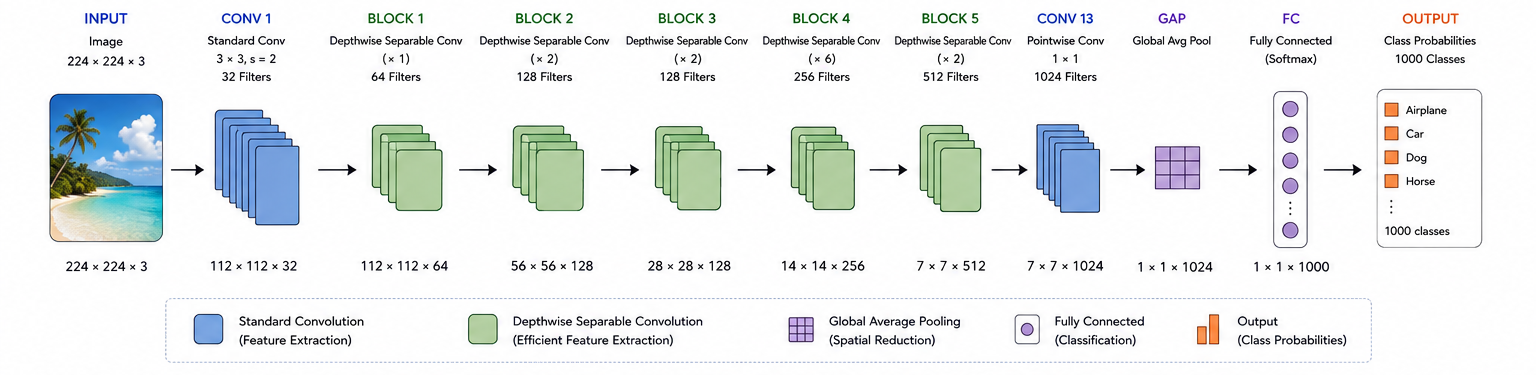
\includegraphics[width=0.95\textwidth]{figures/mobilenet1.png}
\end{figure}
 \begin{figure}[H]
\centering
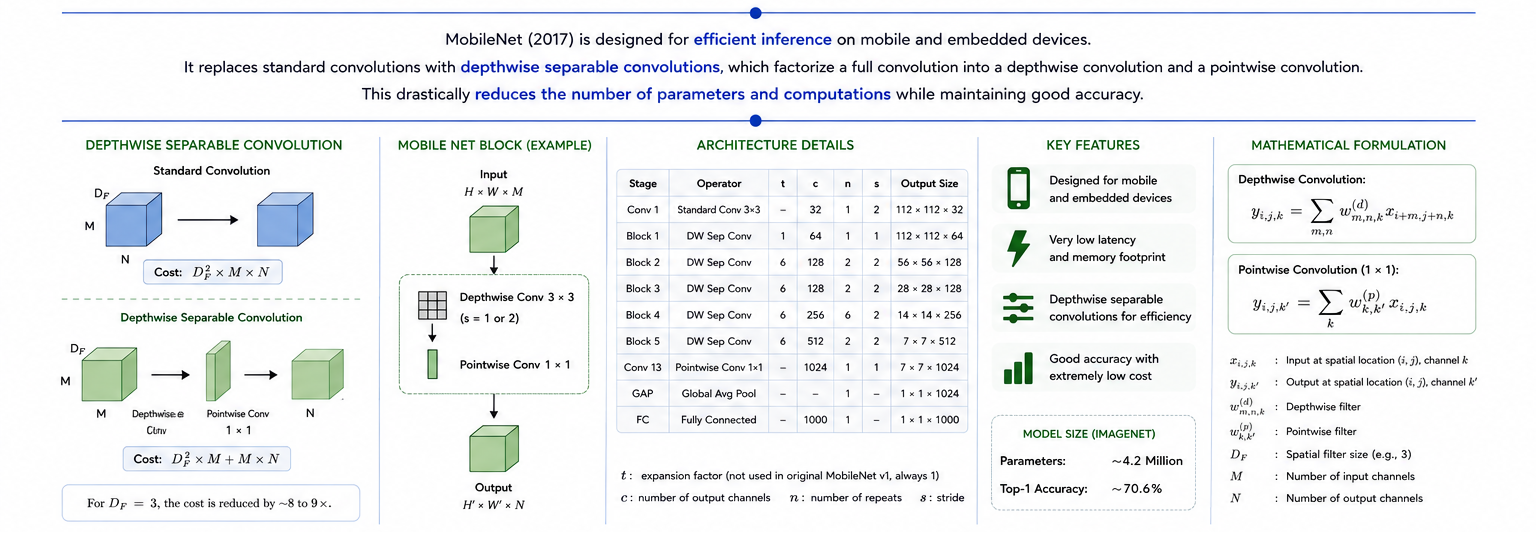
\includegraphics[width=0.95\textwidth]{figures/mobilenet2.png}
\end{figure}

\addtocontents{toc}{\protect\setcounter{tocdepth}{1}}
\chapter{Recurrent Neural Networks (RNN) \& Sequence Models}

\section{Introduction to Sequence Data \& Word Representations}

Standard Feedforward Neural Networks (ANNs) and Convolutional Neural Networks (CNNs) assume that all input samples are independent and identically distributed (i.i.d.). However, real-world data such as text, speech, time-series measurements, financial stocks, and genomic sequences possess temporal or sequential structure where order matters fundamentally.

Before feeding discrete categorical entities like text words into neural networks, they must be converted into numerical vectors.

\subsection{Encoding Strategies: One-Hot vs. Integer Encoding}

Consider two basic approaches to numerical encoding:

\begin{enumerate}
    \item \textbf{Integer Encoding:} Assigning an arbitrary integer ID to each unique word in a dictionary (e.g., $\text{US} = 1, \text{China} = 2, \text{India} = 3$).
    
    \begin{propertybox}[Failure of Integer Encoding]
    Integer encoding introduces arbitrary algebraic ordering and distance relationships that do not exist in language:
    \begin{equation}
    \text{US} + \text{China} = 1 + 2 = 3 = \text{India}
    \end{equation}
    Neural network layers multiply inputs by continuous weights ($W \cdot x$), turning these arbitrary numerical relationships into invalid semantic biases.
    \end{propertybox}

    \item \textbf{One-Hot Encoding:} Representing each word as a sparse binary vector in $\mathbb{R}^V$ (where $V$ is vocabulary size) with a single $1$ at the word's index and $0$ elsewhere:
    \begin{equation}
    e_{\text{king}} = \begin{bmatrix} 1 \\ 0 \\ 0 \\ \vdots \\ 0 \end{bmatrix}, \quad
    e_{\text{queen}} = \begin{bmatrix} 0 \\ 1 \\ 0 \\ \vdots \\ 0 \end{bmatrix}, \quad
    e_{\text{apple}} = \begin{bmatrix} 0 \\ 0 \\ 1 \\ \vdots \\ 0 \end{bmatrix}
    \end{equation}
\end{enumerate}

\begin{advbox}[One-Hot Encoding Limitations]
\textbf{Limitations of One-Hot Vectors:}
\begin{itemize}
    \item \textbf{High Dimensionality \& Sparsity:} For a modest vocabulary size $V = 100,000$, every word vector has length $100,000$ with $99.999\%$ zeros (e.g., $x \in \mathbb{R}^{100000}$).
    \item \textbf{Lack of Semantic Similarity:} Standard basis vectors are orthogonal:
    \begin{equation}
    e_i^T e_j = 0 \quad \forall i \neq j \implies \text{Cosine Similarity}(\text{king}, \text{queen}) = 0
    \end{equation}
    The network cannot infer that "king" and "queen" share semantic properties while "apple" is distinct.
\end{itemize}
\end{advbox}

\subsection{Text Data Processing Pipeline}

To prepare raw text for recurrent neural networks, data passes through a 7-step processing pipeline:

\begin{enumerate}
    \item \textbf{Tokenization:} Split raw text into tokens (words or characters), e.g., \textit{"to be or not to be"}.
    \item \textbf{Count Word Frequencies:} Compute occurrence statistics across the text corpus.
    \item \textbf{Sort by Frequency:} Order tokens from highest frequency to lowest.
    \item \textbf{Build Vocabulary:} Select the top $V$ most frequent words to construct the dictionary.
    \item \textbf{Assign Word Indices:} Map each unique token to an integer ID ($1 \dots V$).
    \item \textbf{Vector Encoding:} Convert integer IDs to One-Hot vectors or dense Embeddings.
    \item \textbf{Unknown Word Token:} Map out-of-vocabulary words to a special unknown token, $\langle \text{UNK} \rangle$.
\end{enumerate}
\begin{figure}[H]
    \centering
    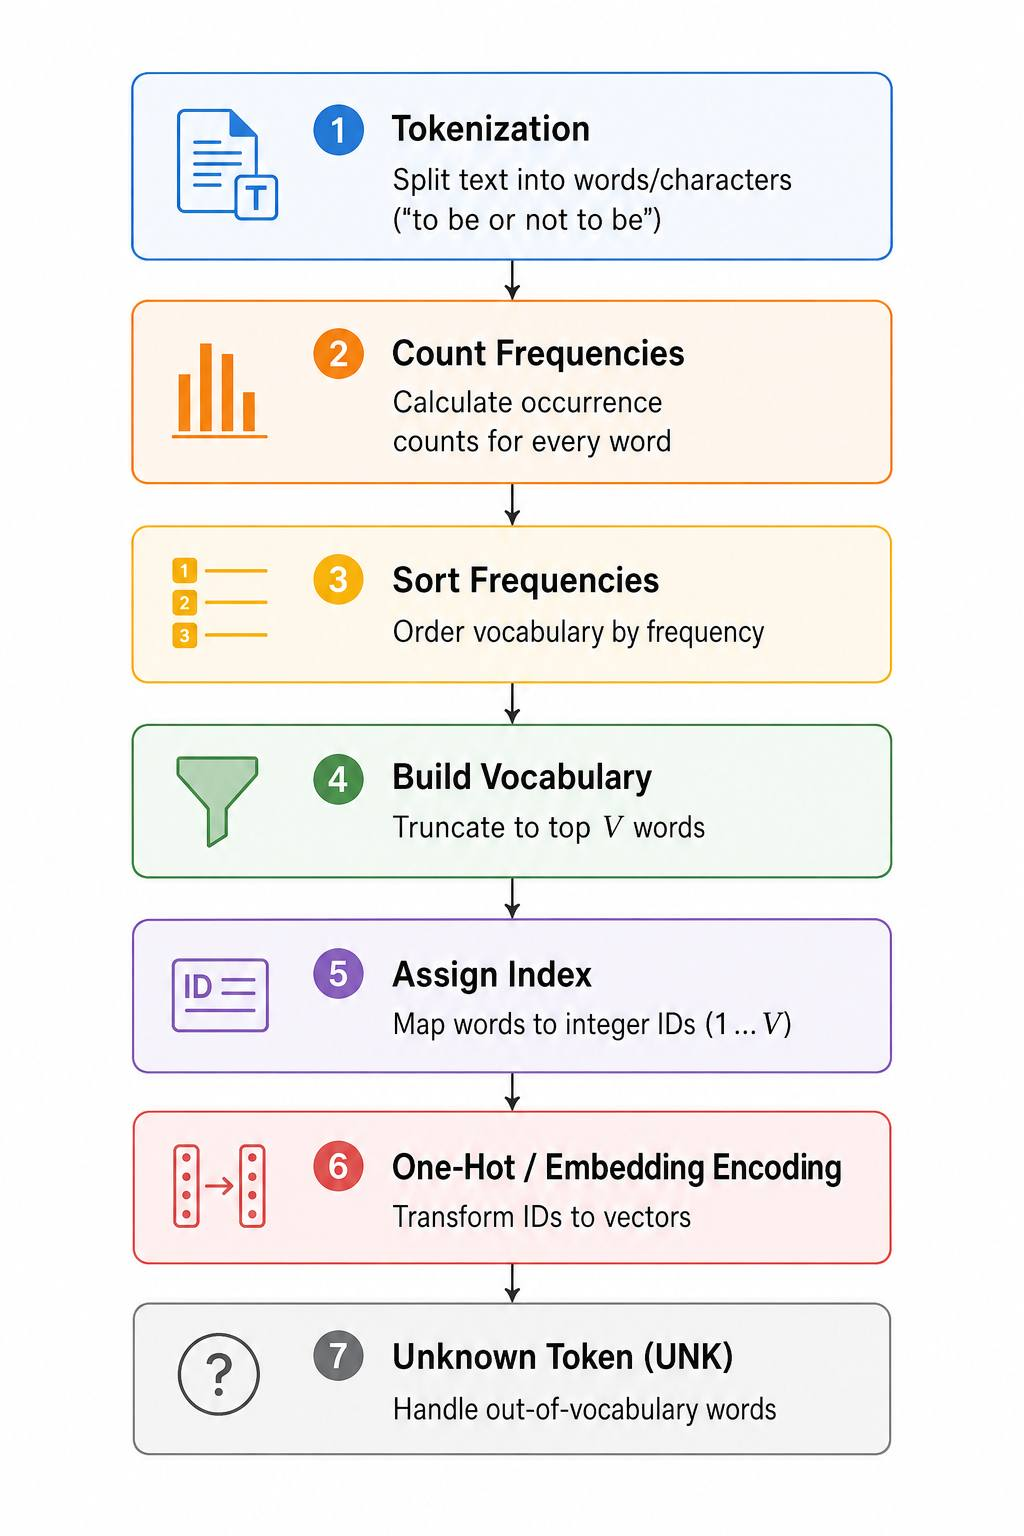
\includegraphics[width=0.95\textwidth]{figures/last.jpg}
\end{figure}

\subsection{Word Embedding Vectors}

Word Embeddings resolve the limitations of One-Hot encoding by projecting discrete words into a dense, low-dimensional continuous vector space $\mathbb{R}^d$ (typically $d \ll V$, e.g., $d \in [50, 300]$).

\begin{equation}
x_{\text{word}} = E \cdot e_{\text{word}}
\end{equation}
where $E \in \mathbb{R}^{d \times V}$ is the learnable embedding matrix.

Dense embeddings capture continuous semantic relationships:
\begin{equation}
v_{\text{king}} - v_{\text{man}} + v_{\text{woman}} \approx v_{\text{queen}}
\end{equation}

\begin{advbox}[Advantages of Word Embeddings]
\begin{itemize}
    \item \textbf{Dense Representation:} Low-dimensional vector space $\mathbb{R}^d$ ($d \ll V$).
    \item \textbf{Continuous Space:} Allows smooth gradient propagation during backpropagation.
    \item \textbf{Semantic Similarities:} Words with similar meanings sit close to each other in vector space.
\end{itemize}
\end{advbox}

\section{Cosine Similarity \& Vector Metrics}

To quantify semantic closeness between vector representations $A, B \in \mathbb{R}^d$, we measure the cosine of the angle $\theta$ between them:

\begin{equation}
\text{Cosine Similarity}(A, B) = \cos(\theta) = \frac{A \cdot B}{\|A\| \|B\|} = \frac{\sum_{i=1}^d A_i B_i}{\sqrt{\sum_{i=1}^d A_i^2} \sqrt{\sum_{i=1}^d B_i^2}}
\end{equation}

\begin{figure}[htbp]
\centering
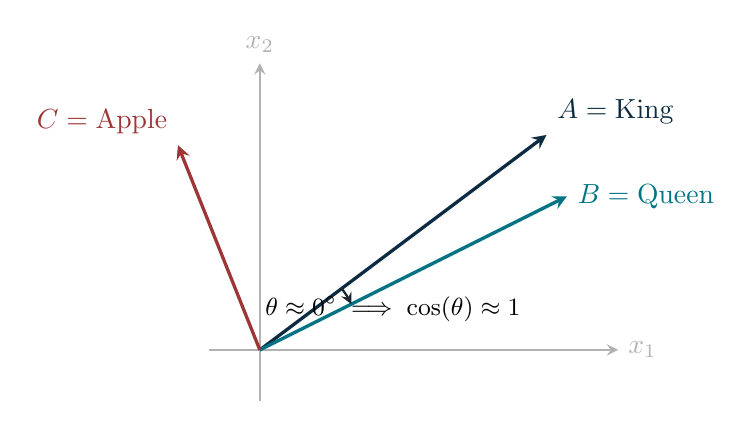
\begin{tikzpicture}[scale=1.3, >=stealth]
    % Axes
    \draw[->, color=gray!60, thick] (-0.5,0) -- (3.5,0) node[right] {$x_1$};
    \draw[->, color=gray!60, thick] (0,-0.5) -- (0,2.8) node[above] {$x_2$};
    
    % Vectors
    \draw[->, very thick, primaryblue] (0,0) -- (2.8, 2.1) node[above right] {$A = \text{King}$};
    \draw[->, very thick, secondaryblue] (0,0) -- (3.0, 1.5) node[right] {$B = \text{Queen}$};
    \draw[->, very thick, accentred] (0,0) -- (-0.8, 2.0) node[above left] {$C = \text{Apple}$};
    
    % Angle arc
    \draw[->, thick, darkslate] (0.8,0.6) arc (36.87:26.56:1.0);
    \node at (1.3, 0.4) {\small $\theta \approx 0^\circ \implies \cos(\theta) \approx 1$};
\end{tikzpicture}
\caption{Vector Space Geometry: Cosine Similarity measures directional alignment in embedding space.}
\label{fig:cosine_geometry_ch3}
\end{figure}

\begin{propertybox}[Interpretation of Cosine Similarity Values]
\begin{itemize}
    \item \textbf{$+1$ (Identical Direction):} Vectors point in exactly the same direction ($\theta = 0^\circ$). High semantic similarity (e.g., $\text{Cosine Similarity}(\text{King}, \text{Queen}) = 0.98$).
    \item \textbf{$0$ (Orthogonal):} Vectors are independent ($\theta = 90^\circ$). No semantic relationship.
    \item \textbf{$-1$ (Opposite Direction):} Vectors point in diametrically opposite directions ($\theta = 180^\circ$). Opposing semantic meanings.
\end{itemize}
\end{propertybox}

\section{Recurrent Neural Network (RNN) Fundamentals}

\subsection{Why Standard Neural Networks Fail on Sequential Data}

Standard Feedforward Neural Networks (ANNs) and Convolutional Networks (CNNs) fail on sequential domain data (e.g., text, speech, time-series, DNA, financial stocks) because:
\begin{enumerate}
    \item Inputs and outputs can have variable sequence length $T$.
    \item Context from prior time steps is lost. Permuting word order completely alters meaning:
    \begin{center}
    \textit{"I love deep learning"} \quad vs. \quad \textit{"learning deep love I"}
    \end{center}
    \item Standard networks lack temporal memory and parameter sharing across time steps.
\end{enumerate}
\subsection{Hidden State Update Equations}

To maintain memory across time steps, an RNN maintains a temporal \textbf{hidden state} $h_t$ updated at each step $t$:

\begin{equation}
h_t = \phi(W_{hh} h_{t-1} + W_{xh} x_t + b_h)
\end{equation}
\begin{figure}[H]
    \centering
    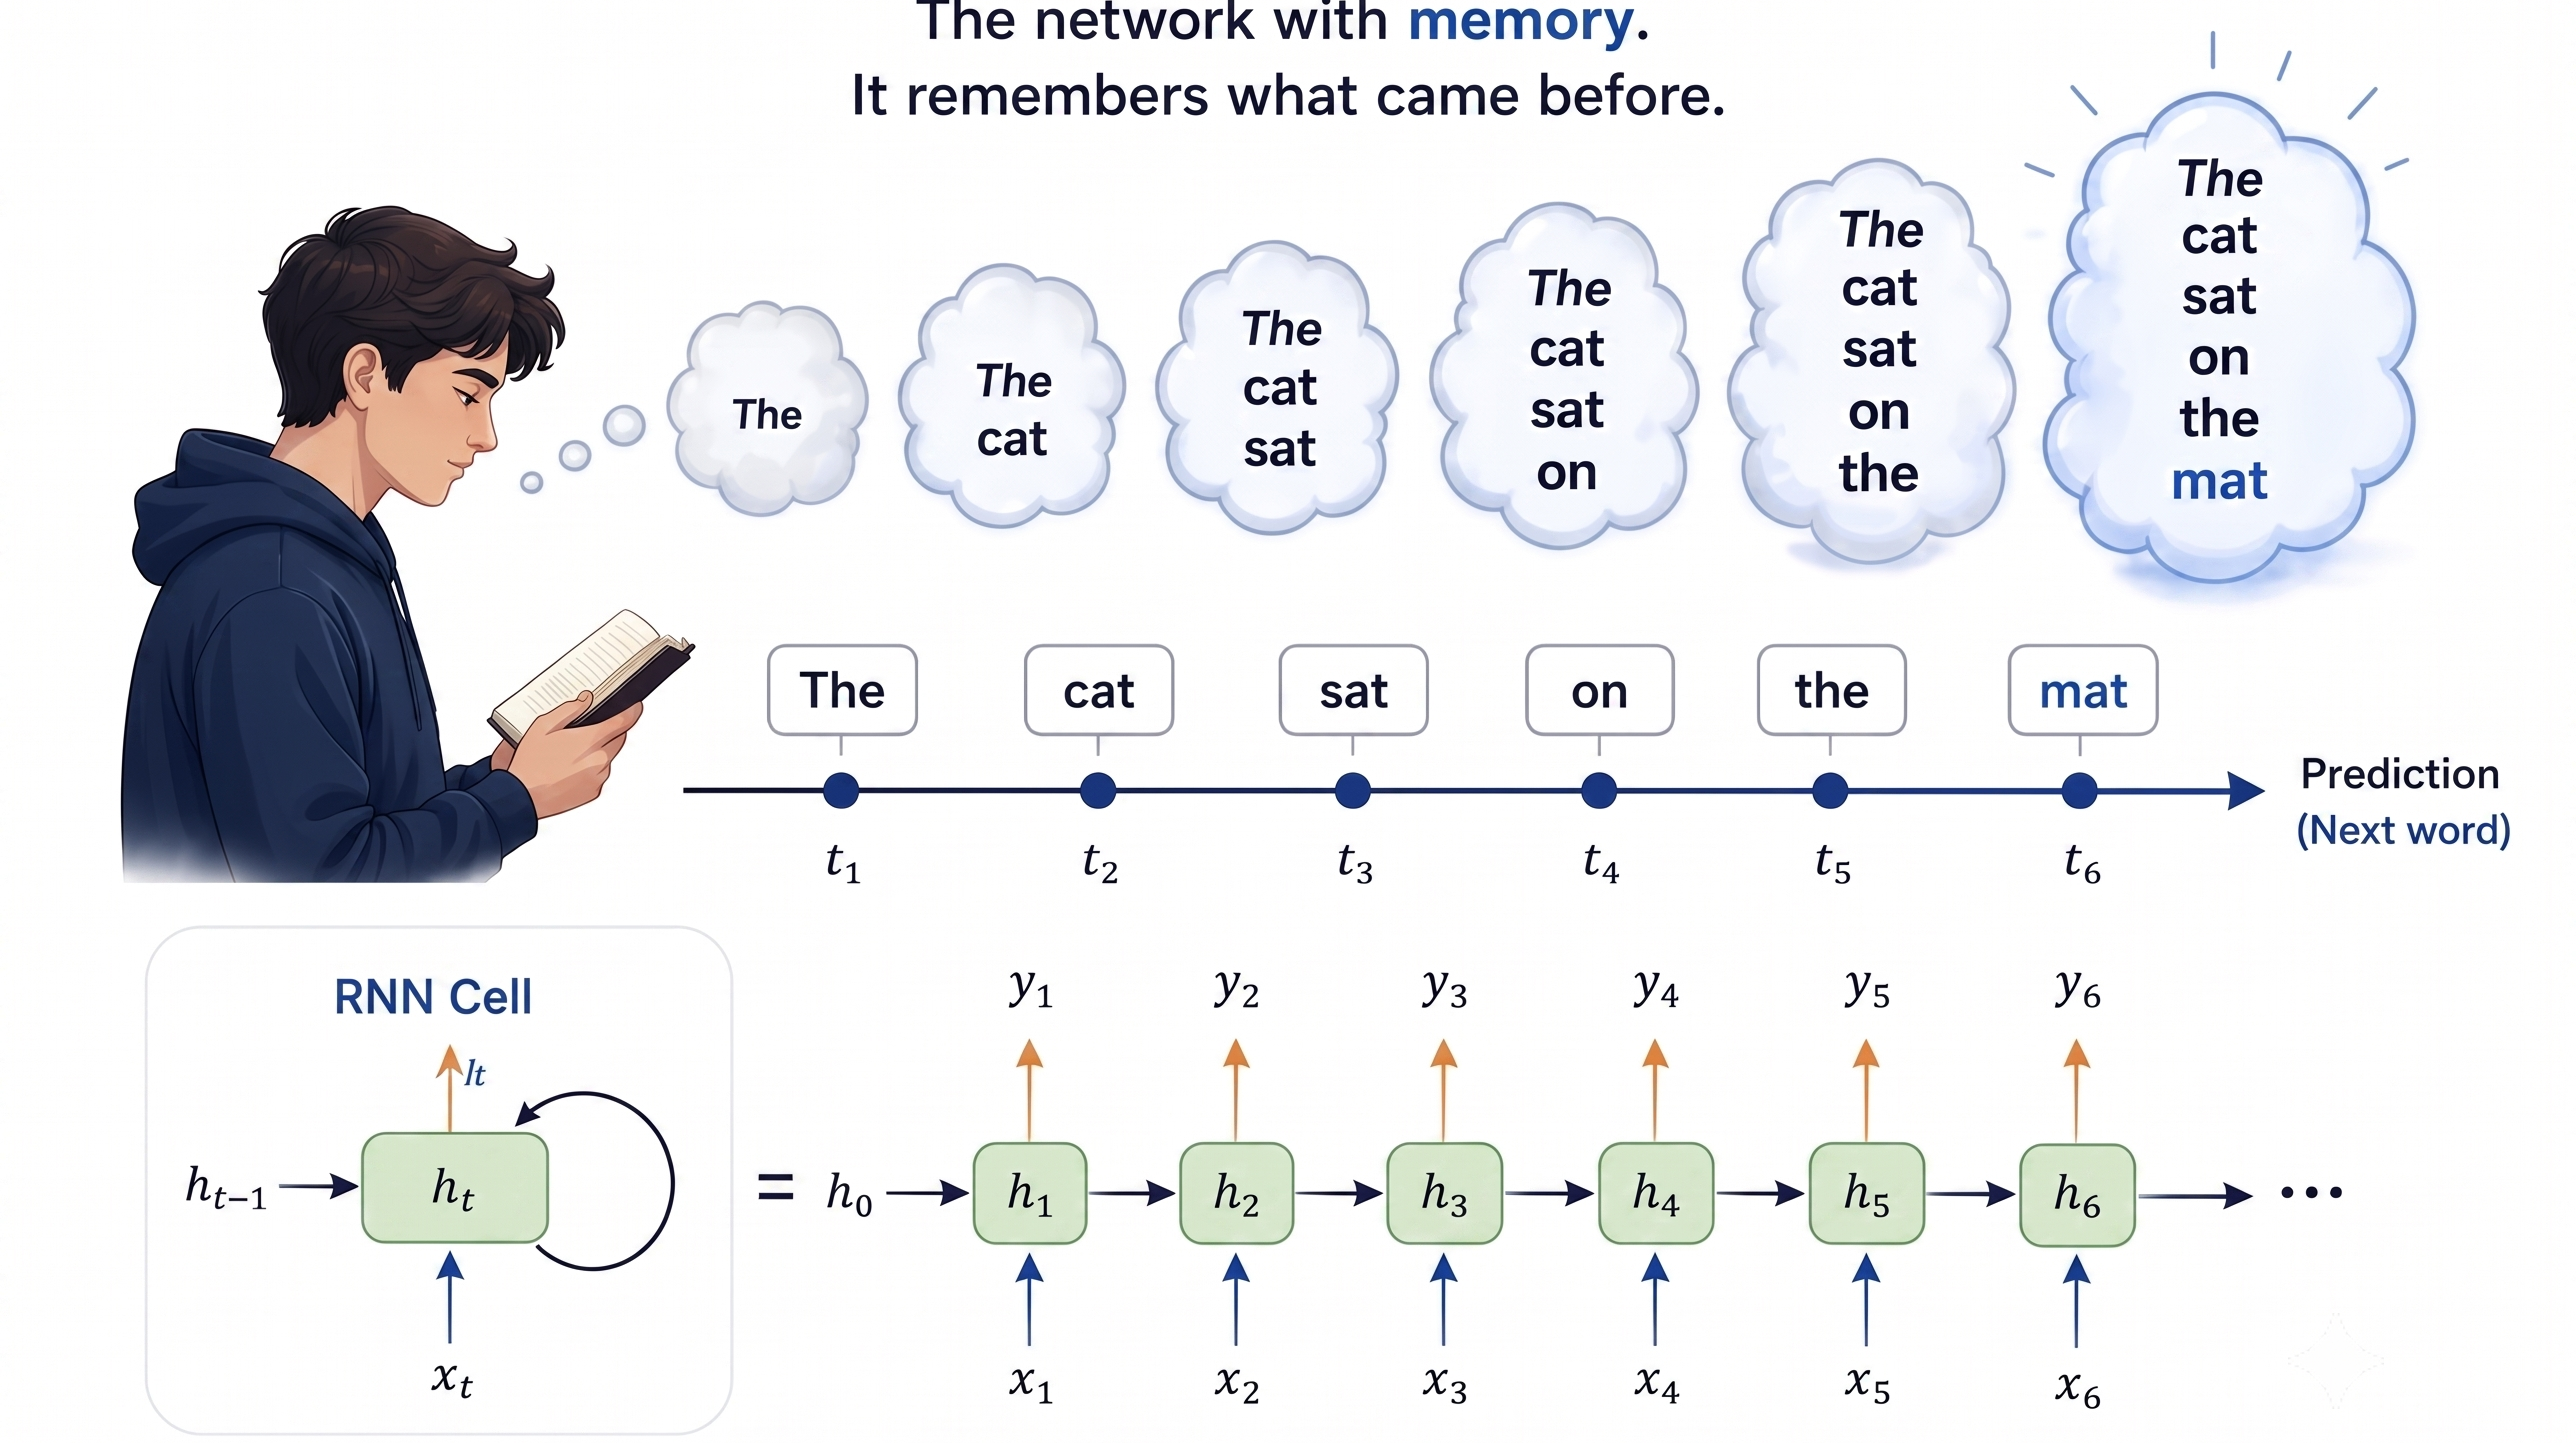
\includegraphics[width=0.95\textwidth]{figures/rnn.png}
\end{figure}
At each time step $t$, the output $y_t$ is computed from hidden state $h_t$:

\begin{equation}
y_t = g(W_{hy} h_t + b_y)
\end{equation}
where $g$ is the output activation function ($g \in \{\text{sigmoid}, \text{softmax}, \text{linear}\}$).

\begin{propertybox}[Parameter Sharing Across Time Steps]
The weight matrices $W_{hh}, W_{xh}$, and $W_{hy}$ are \textbf{shared across all time steps}. The exact same parameters process the transition between $x_1 \to h_1, x_2 \to h_2$, and $x_3 \to h_3$.
\end{propertybox}

\begin{figure}[htbp]
\centering
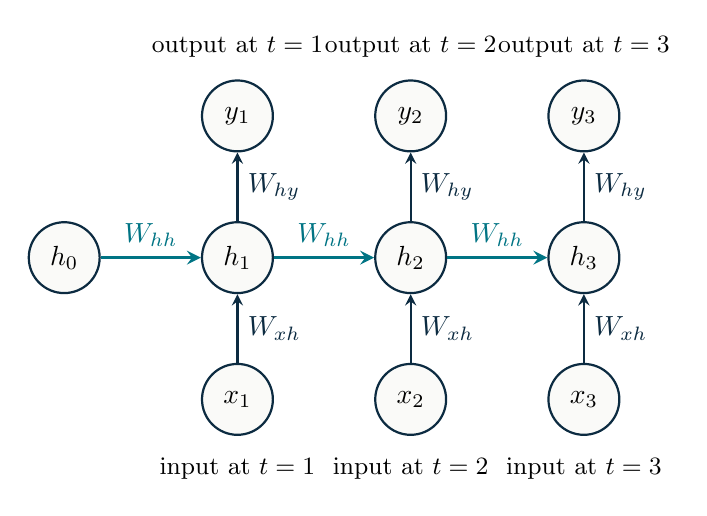
\begin{tikzpicture}[node distance=2.2cm, >=stealth, auto]
    % Initial state h0
    \node[circle, draw=primaryblue, fill=lightbg, thick, minimum size=0.9cm] (h0) {$h_0$};
    
    % Hidden states h1, h2, h3
    \node[circle, draw=primaryblue, fill=lightbg, thick, minimum size=0.9cm, right of=h0] (h1) {$h_1$};
    \node[circle, draw=primaryblue, fill=lightbg, thick, minimum size=0.9cm, right of=h1] (h2) {$h_2$};
    \node[circle, draw=primaryblue, fill=lightbg, thick, minimum size=0.9cm, right of=h2] (h3) {$h_3$};
    
    % Inputs x1, x2, x3
    \node[circle, draw=primaryblue, fill=lightbg, thick, minimum size=0.9cm, below of=h1, node distance=1.8cm] (x1) {$x_1$};
    \node[circle, draw=primaryblue, fill=lightbg, thick, minimum size=0.9cm, below of=h2, node distance=1.8cm] (x2) {$x_2$};
    \node[circle, draw=primaryblue, fill=lightbg, thick, minimum size=0.9cm, below of=h3, node distance=1.8cm] (x3) {$x_3$};
    
    % Outputs y1, y2, y3
    \node[circle, draw=primaryblue, fill=lightbg, thick, minimum size=0.9cm, above of=h1, node distance=1.8cm] (y1) {$y_1$};
    \node[circle, draw=primaryblue, fill=lightbg, thick, minimum size=0.9cm, above of=h2, node distance=1.8cm] (y2) {$y_2$};
    \node[circle, draw=primaryblue, fill=lightbg, thick, minimum size=0.9cm, above of=h3, node distance=1.8cm] (y3) {$y_3$};
    
    % Labels for inputs and outputs
    \node[below=0.15cm of x1, font=\small] {input at $t=1$};
    \node[below=0.15cm of x2, font=\small] {input at $t=2$};
    \node[below=0.15cm of x3, font=\small] {input at $t=3$};
    
    \node[above=0.15cm of y1, font=\small] {output at $t=1$};
    \node[above=0.15cm of y2, font=\small] {output at $t=2$};
    \node[above=0.15cm of y3, font=\small] {output at $t=3$};
    
    % Input arrows
    \draw[->, thick, primaryblue] (x1) -- (h1) node[midway, right] {$W_{xh}$};
    \draw[->, thick, primaryblue] (x2) -- (h2) node[midway, right] {$W_{xh}$};
    \draw[->, thick, primaryblue] (x3) -- (h3) node[midway, right] {$W_{xh}$};
    
    % Recurrent arrows
    \draw[->, very thick, secondaryblue] (h0) -- (h1) node[midway, above] {$W_{hh}$};
    \draw[->, very thick, secondaryblue] (h1) -- (h2) node[midway, above] {$W_{hh}$};
    \draw[->, very thick, secondaryblue] (h2) -- (h3) node[midway, above] {$W_{hh}$};
    
    % Output arrows
    \draw[->, thick, primaryblue] (h1) -- (y1) node[midway, right] {$W_{hy}$};
    \draw[->, thick, primaryblue] (h2) -- (y2) node[midway, right] {$W_{hy}$};
    \draw[->, thick, primaryblue] (h3) -- (y3) node[midway, right] {$W_{hy}$};
\end{tikzpicture}
\caption{Unrolled Simple Recurrent Neural Network Computational Graph (Page 56).}
\label{fig:simple_rnn_unrolled_custom}
\end{figure}

\section{Sequence Topologies \& Encoder-Decoder Models}

Recurrent neural networks flex to match different task structures, as categorized by Andrej Karpathy:

\begin{enumerate}
    \item \textbf{One-to-One:} Standard fixed input to fixed output ($y = f(x)$).
    \item \textbf{One-to-Many:} Single input produces sequence output (e.g., Image Captioning, Music Generation).
    \item \textbf{Many-to-One:} Sequence input produces single output (e.g., Sentiment Analysis, Text Classification).
    \item \textbf{Many-to-Many (Synchronized):} Sequence input produces synchronized sequence output of same length $T$ (e.g., Video Frame Labeling, POS Tagging).
    \item \textbf{Many-to-Many (Asynchronous / Encoder-Decoder):} Sequence input of length $T_x$ produces sequence output of length $T_y$ (e.g., Machine Translation).
\end{enumerate}

\begin{figure}[htbp]
\centering
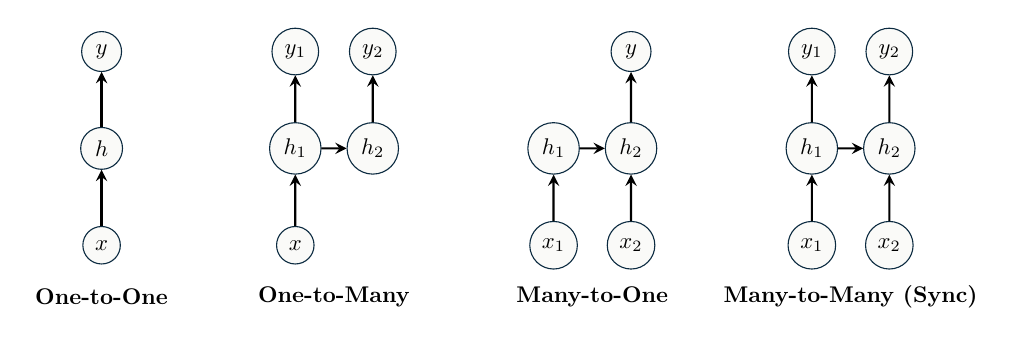
\begin{tikzpicture}[scale=0.82, transform shape, >=stealth]
    % 1-to-1
    \node[draw=primaryblue, fill=lightbg, circle] (x11) at (0,0) {$x$};
    \node[draw=primaryblue, fill=lightbg, circle] (h11) at (0,1.5) {$h$};
    \node[draw=primaryblue, fill=lightbg, circle] (y11) at (0,3.0) {$y$};
    \draw[->, thick] (x11)--(h11); \draw[->, thick] (h11)--(y11);
    \node at (0,-0.8) {\textbf{One-to-One}};

    % 1-to-Many
    \node[draw=primaryblue, fill=lightbg, circle] (x21) at (3,0) {$x$};
    \node[draw=primaryblue, fill=lightbg, circle] (h21) at (3,1.5) {$h_1$};
    \node[draw=primaryblue, fill=lightbg, circle] (h22) at (4.2,1.5) {$h_2$};
    \node[draw=primaryblue, fill=lightbg, circle] (y21) at (3,3.0) {$y_1$};
    \node[draw=primaryblue, fill=lightbg, circle] (y22) at (4.2,3.0) {$y_2$};
    \draw[->, thick] (x21)--(h21); \draw[->, thick] (h21)--(h22);
    \draw[->, thick] (h21)--(y21); \draw[->, thick] (h22)--(y22);
    \node at (3.6,-0.8) {\textbf{One-to-Many}};

    % Many-to-1
    \node[draw=primaryblue, fill=lightbg, circle] (x31) at (7,0) {$x_1$};
    \node[draw=primaryblue, fill=lightbg, circle] (x32) at (8.2,0) {$x_2$};
    \node[draw=primaryblue, fill=lightbg, circle] (h31) at (7,1.5) {$h_1$};
    \node[draw=primaryblue, fill=lightbg, circle] (h32) at (8.2,1.5) {$h_2$};
    \node[draw=primaryblue, fill=lightbg, circle] (y32) at (8.2,3.0) {$y$};
    \draw[->, thick] (x31)--(h31); \draw[->, thick] (x32)--(h32);
    \draw[->, thick] (h31)--(h32); \draw[->, thick] (h32)--(y32);
    \node at (7.6,-0.8) {\textbf{Many-to-One}};

    % Many-to-Many Sync
    \node[draw=primaryblue, fill=lightbg, circle] (x41) at (11,0) {$x_1$};
    \node[draw=primaryblue, fill=lightbg, circle] (x42) at (12.2,0) {$x_2$};
    \node[draw=primaryblue, fill=lightbg, circle] (h41) at (11,1.5) {$h_1$};
    \node[draw=primaryblue, fill=lightbg, circle] (h42) at (12.2,1.5) {$h_2$};
    \node[draw=primaryblue, fill=lightbg, circle] (y41) at (11,3.0) {$y_1$};
    \node[draw=primaryblue, fill=lightbg, circle] (y42) at (12.2,3.0) {$y_2$};
    \draw[->, thick] (x41)--(h41); \draw[->, thick] (x42)--(h42);
    \draw[->, thick] (h41)--(h42);
    \draw[->, thick] (h41)--(y41); \draw[->, thick] (h42)--(y42);
    \node at (11.6,-0.8) {\textbf{Many-to-Many (Sync)}};
\end{tikzpicture}
\caption{RNN Sequence Topologies (Karpathy).}
\label{fig:topologies_ch3}
\end{figure}
\clearpage
\section{Backpropagation Through Time (BPTT)}

Backpropagation Through Time (BPTT) extends standard backpropagation by unrolling the recurrent network through time and computing gradients across all time steps.

\begin{figure}[htbp]
\centering
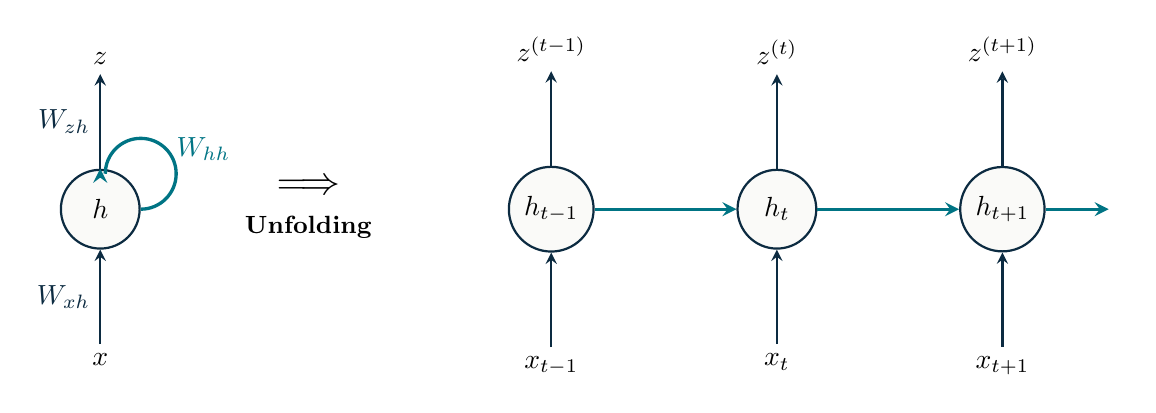
\begin{tikzpicture}[node distance=1.8cm, >=stealth, auto,
    state/.style={circle, draw=primaryblue, fill=lightbg, thick, minimum size=1.0cm},
    arrow/.style={->, thick, primaryblue},
    recarrow/.style={->, very thick, secondaryblue}
]
    % Left side: Folded view
    \node[state] (h_folded) {$h$};
    \node[below=1.2cm of h_folded] (x_folded) {$x$};
    \node[above=1.2cm of h_folded] (z_folded) {$z$};
    
    \draw[arrow] (x_folded) -- (h_folded) node[midway, left] {$W_{xh}$};
    \draw[arrow] (h_folded) -- (z_folded) node[midway, left] {$W_{zh}$};
    \draw[recarrow] (h_folded.east) arc (-90:180:0.45cm) node[midway, right] {$W_{hh}$} (h_folded.north);
    
    % Unfolding Arrow
    \node[right=1.2cm of h_folded, align=center] (unfold) {\Large $\Longrightarrow$\\[0.2em] \small \textbf{Unfolding}};
    
    % Right side: Unrolled view
    \node[state, right=1.6cm of unfold] (h_t1) {$h_{t-1}$};
    \node[state, right=1.8cm of h_t1] (h_t) {$h_t$};
    \node[state, right=1.8cm of h_t] (h_t2) {$h_{t+1}$};
    \node[right=0.8cm of h_t2] (dots) {};
    
    \node[below=1.2cm of h_t1] (x_t1) {$x_{t-1}$};
    \node[below=1.2cm of h_t] (x_t) {$x_t$};
    \node[below=1.2cm of h_t2] (x_t2) {$x_{t+1}$};
    
    \node[above=1.2cm of h_t1] (z_t1) {$z^{(t-1)}$};
    \node[above=1.2cm of h_t] (z_t) {$z^{(t)}$};
    \node[above=1.2cm of h_t2] (z_t2) {$z^{(t+1)}$};
    
    \draw[arrow] (x_t1) -- (h_t1); \draw[arrow] (x_t) -- (h_t); \draw[arrow] (x_t2) -- (h_t2);
    \draw[arrow] (h_t1) -- (z_t1); \draw[arrow] (h_t) -- (z_t); \draw[arrow] (h_t2) -- (z_t2);
    \draw[recarrow] (h_t1) -- (h_t); \draw[recarrow] (h_t) -- (h_t2); \draw[recarrow] (h_t2) -- (dots);
\end{tikzpicture}
\caption{Backpropagation Through Time (BPTT) Unrolled Graph.}
\label{fig:bptt_diagram_custom}
\end{figure}
\clearpage
\section{Long Short-Term Memory (LSTM)}

\textbf{LSTM:}

The Long Short-Term Memory (LSTM) network was proposed in 1997. Its objectives are to:
\begin{itemize}
    \item Preserve information over long sequences.
    \item Reduce the vanishing-gradient problem.
    \item Learn both short-term and long-term dependencies.
    \item Decide automatically which information to keep or discard.
\end{itemize}

Unlike a simple RNN, an LSTM has two states:
\begin{itemize}
    \item \textbf{Hidden state $h_t$:} The short-term memory used to produce outputs.
    \item \textbf{Cell state $C_t$:} The long-term memory that carries information through the sequence.
\end{itemize}

\begin{propertybox}[Key Concept]
The cell state carries the LSTM's key information.
\end{propertybox}

\begin{figure}[htbp]
\centering
\includegraphics[width=0.95\textwidth]{3-RNN/lstm_cell.png}
\caption{Detailed Long Short-Term Memory (LSTM) Cell Architecture.}
\label{fig:lstm_cell_detailed_custom}
\end{figure}

\subsection{Cell State}

\textbf{Cell state:} A vector denoted by $C_t$ that stores long-term information across time steps. Unlike the hidden state, the cell state is designed to let information flow through many time steps with only small modifications. Often described as a ``memory highway,'' it is updated gradually from $C_{t-1}$ to $C_t$ rather than being completely recomputed at every step.

The gates decide how much information is forgotten, added, or exposed.

\begin{advbox}[Intuition]
Imagine reading a book:
\begin{itemize}
    \item You remember the main story (cell state)
    \item You temporarily focus on the current sentence (hidden state)
\end{itemize}
The cell state acts like long-term memory, while the hidden state represents the current understanding.
\end{advbox}

\subsection{LSTM Gates}

An LSTM contains three gates:
\begin{enumerate}
    \item Forget gate
    \item Input gate
    \item Output gate
\end{enumerate}

Each gate is implemented using the sigmoid activation function $\sigma(x) = \frac{1}{1 + e^{-x}}$, where $0 \le \sigma(x) \le 1$.
\begin{itemize}
    \item \textbf{0:} completely block the information
    \item \textbf{1:} pass all the information
    \item \textbf{intermediate values $\to$} partially pass information
\end{itemize}
The gates behave like intelligent switches.

\subsubsection{I) Forget Gate}

The forget gate determines which information from the previous cell state should be retained. It computes:
\begin{equation}
f_t = \sigma(W_f [h_{t-1}, x_t] + b_f)
\end{equation}
where:
\begin{itemize}
    \item $W_f$: forget-gate weight matrix
    \item $b_f$: forget-gate bias
    \item $[h_{t-1}, x_t]$: concatenation of the previous hidden state and current input.
\end{itemize}

\begin{itemize}
    \item If $f_t = 1$, the previous memory is fully preserved.
    \item If $f_t = 0$, the previous memory is completely erased.
    \item If $f_t = 0.4$, 40\% is retained.
\end{itemize}

\subsubsection{II) Input Gate}

The input gate determines which new information should be stored. It has two parts:
\begin{enumerate}
    \item \textbf{Gate Activation:} $i_t = \sigma(W_i [h_{t-1}, x_t] + b_i)$
    \item \textbf{Candidate Memory:} $\tilde{C}_t = \tanh(W_c [h_{t-1}, x_t] + b_c)$
\end{enumerate}

The candidate memory contains the new information that may be written into the cell state.

\begin{propertybox}[Input Gate Example]
Example $i_t = \begin{bmatrix} 1 \\ 0.3 \end{bmatrix}$ and $\tilde{C}_t = \begin{bmatrix} 2 \\ 5 \end{bmatrix}$ then $i_t \otimes \tilde{C}_t = \begin{bmatrix} 2 \\ 1.5 \end{bmatrix}$.\\
Only a fraction of the second candidate value is stored.
\end{propertybox}

\subsubsection{III) Output Gate}

The output gate determines which information from the cell state becomes the hidden state.
\begin{align}
\text{First: } & o_t = \sigma(W_o [h_{t-1}, x_t] + b_o) \\
\text{Then: } & h_t = o_t \otimes \tanh(C_t)
\end{align}

The hidden state $h_t$ is:
\begin{itemize}
    \item passed to the next LSTM cell
    \item used to compute the next network's output.
\end{itemize}

\subsubsection{IV) Cell State Update}

The cell state is updated by combining the retained old memory with the selected new memory:
\begin{equation}
C_t = f_t \otimes C_{t-1} + i_t \otimes \tilde{C}_t
\end{equation}
This is the central equation of the LSTM.

\begin{propertybox}[Complete Forward Pass]
\begin{align}
f_t &= \sigma(W_f [h_{t-1}, x_t] + b_f) \\
i_t &= \sigma(W_i [h_{t-1}, x_t] + b_i) \\
\tilde{C}_t &= \tanh(W_c [h_{t-1}, x_t] + b_c) \\
C_t &= f_t \otimes C_{t-1} + i_t \otimes \tilde{C}_t \\
o_t &= \sigma(W_o [h_{t-1}, x_t] + b_o) \\
h_t &= o_t \otimes \tanh(C_t)
\end{align}
These six equations define a standard LSTM cell.
\end{propertybox}

\subsection{Complexity \& Why LSTM Works}

\textbf{Complexity:} Four matrix multiplications
\begin{equation}
\mathcal{O}(4(n_x n_h + n_h^2)) \sim \mathcal{O}(n_x n_h + n_h^2)
\end{equation}
For a sequence of length $T$:
\begin{equation}
\mathcal{O}(T(n_x n_h + n_h^2))
\end{equation}
Compared with a simple RNN, an LSTM is roughly four times more expensive per time step because it computes four gates instead of one hidden-state update.

\textbf{LSTMs work because:}
\begin{itemize}
    \item \textbf{The forget gate:} removes irrelevant information
    \item \textbf{The input gate:} writes useful new information
    \item \textbf{The output gate:} decides what information should influence the current prediction
\end{itemize}
Because the cell-state update contains an additive term $C_t = f_t \otimes C_{t-1} + i_t \otimes \tilde{C}_t$, gradients can propagate through many time steps more effectively than in a simple RNN, greatly reducing the vanishing-gradient problem. Although LSTMs do not completely eliminate gradient issues, they are better able to learn long-range dependencies.

\subsection{Advantages \& Limitations}

\begin{advbox}[Advantages]
\begin{itemize}
    \item Captures long-term dependencies
    \item Greatly reduces the vanishing gradient problem
    \item Learns which information to remember and which to forget
    \item Performs well on NLP, speech recognition, and machine translation
    \item Supports variable-length input sequences
\end{itemize}
\end{advbox}

\begin{advbox}[Limitations]
\begin{itemize}
    \item More parameters than a simple RNN, increasing memory requirements
    \item Higher computational cost due to the four gates
    \item Longer training times
    \item More difficult to interpret because multiple gates interact simultaneously
\end{itemize}
\end{advbox}

\section{Gated Recurrent Unit (GRU)}

\textbf{Introduction:} The GRU is a recurrent neural network architecture introduced in 2014 as a simplified alternative to the LSTM.

\textbf{The main objectives of the GRU are to:}
\begin{itemize}
    \item Learn long-term dependencies
    \item Reduce the vanishing gradient problem
    \item Simplify the LSTM architecture
    \item Reduce the number of trainable parameters
    \item Train faster while achieving comparable performance.
\end{itemize}

\textbf{The GRU simplifies the LSTM architecture by:}
\begin{itemize}
    \item Removing the separate cell state
    \item Combining forget and input mechanisms into a single update gate
    \item Keeping only one memory vector: the hidden state.
\end{itemize}

\textbf{The GRU balances simplicity and performance.}

\begin{figure}[htbp]
\centering
\includegraphics[width=0.95\textwidth]{3-RNN/gru_cell.png}
\caption{Conceptual overview of the Gated Recurrent Unit (GRU): one hidden state is selectively reset and blended at each time step.}
\label{fig:gru_architecture_custom_p74}
\end{figure}

\subsection{Update Gate \& Reset Gate}

\subsubsection{II) Update Gate}

The update gate determines how much of the previous hidden state should be retained. It plays a role similar to the combined action of the forget and input gates in an LSTM:
\begin{equation}
z_t = \sigma(W_z x_t + U_z h_{t-1} + b_z) \quad \text{where }
\begin{cases}
W_z: \text{input weights} \\
U_z: \text{recurrent weights} \\
b_z: \text{bias}
\end{cases}, \quad 0 \le z_t \le 1
\end{equation}

The gate controls the proportion of old versus new information:
\begin{itemize}
    \item $z_t = 1$: the previous hidden state is almost preserved
    \item $z_t = 0$: the model ignores the previous state and relies on newly computed information
\end{itemize}

\subsubsection{III) Reset Gate}

The reset gate determines how much of the previous memory should be ignored when computing the new candidate hidden state:
\begin{equation}
r_t = \sigma(W_r x_t + U_r h_{t-1} + b_r)
\end{equation}
\begin{itemize}
    \item $r_t = 0$: the previous hidden state is almost completely ignored
    \item $r_t = 1$: all previous information is considered
\end{itemize}
It is useful when the model needs to discard outdated context and start processing a new pattern.

\subsection{Candidate Hidden State \& Forward Pass}

\textbf{Candidate Hidden State:}
\begin{equation}
\tilde{h}_t = \tanh(W_h x_t + U_h (r_t \otimes h_{t-1}) + b_h)
\end{equation}

The new hidden state is obtained by combining:
\begin{itemize}
    \item the previous hidden state
    \item the candidate hidden state
\end{itemize}

\begin{propertybox}[Complete Forward Pass]
\begin{align}
\text{Update Gate: } & z_t = \sigma(W_z x_t + U_z h_{t-1} + b_z) \\
\text{Reset Gate: } & r_t = \sigma(W_r x_t + U_r h_{t-1} + b_r) \\
\text{Candidate Hidden State: } & \tilde{h}_t = \tanh(W_h x_t + U_h (r_t \otimes h_{t-1}) + b_h) \\
\text{Hidden State: } & h_t = z_t \otimes h_{t-1} + (1 - z_t) \otimes \tilde{h}_t
\end{align}
These four equations completely define the GRU.
\end{propertybox}

\begin{figure}[htbp]
\centering
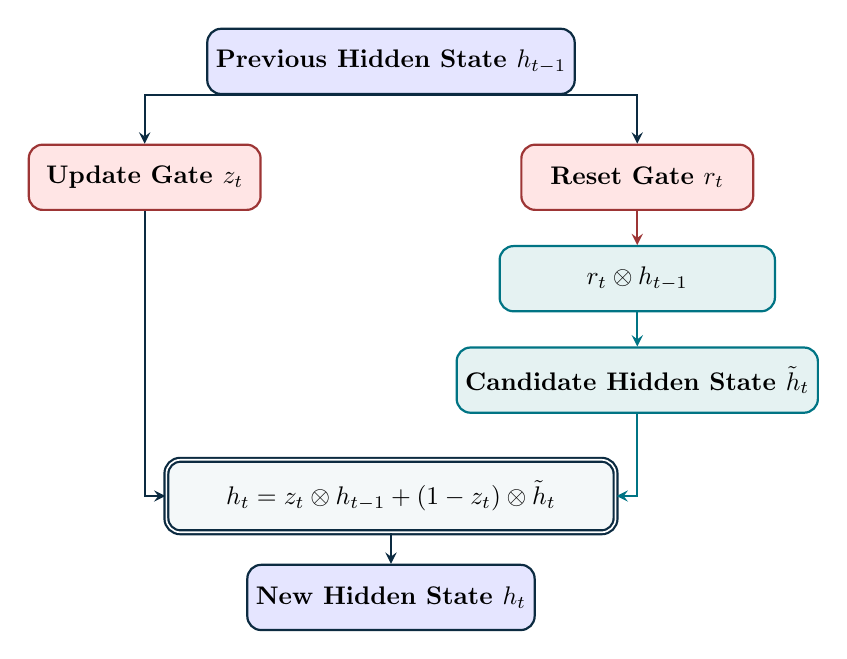
\begin{tikzpicture}[node distance=1.4cm, >=stealth, auto, scale=0.92, transform shape,
    box/.style={rectangle, draw=primaryblue, fill=blue!10, thick, rounded corners=5pt, minimum width=3.8cm, minimum height=0.9cm, align=center},
    gatebox/.style={rectangle, draw=accentred, fill=red!10, thick, rounded corners=5pt, minimum width=3.2cm, minimum height=0.9cm, align=center},
    opbox/.style={rectangle, draw=secondaryblue, fill=teal!10, thick, rounded corners=5pt, minimum width=3.8cm, minimum height=0.9cm, align=center},
    eqbox/.style={rectangle, draw=primaryblue, fill=boxbg, double, thick, rounded corners=5pt, minimum width=6.2cm, minimum height=1.0cm, align=center}
]
    % Top center node
    \node[box] (hprev) at (0, 4.2) {\textbf{Previous Hidden State $h_{t-1}$}};

    % Symmetric Gate branches
    \node[gatebox] (update) at (-3.4, 2.6) {\textbf{Update Gate $z_t$}};
    \node[gatebox] (reset) at (3.4, 2.6) {\textbf{Reset Gate $r_t$}};

    % Under reset gate
    \node[opbox] (reset_state) at (3.4, 1.2) {$r_t \otimes h_{t-1}$};
    \node[opbox] (candidate) at (3.4, -0.2) {\textbf{Candidate Hidden State $\tilde{h}_t$}};

    % Centered Combination equation box
    \node[eqbox] (combine) at (0, -1.8) {$h_t = z_t \otimes h_{t-1} + (1 - z_t) \otimes \tilde{h}_t$};

    % Bottom center node
    \node[box] (hnew) at (0, -3.2) {\textbf{New Hidden State $h_t$}};

    % Symmetric Connecting Arrows
    \draw[->, thick, primaryblue] (hprev.south) -| (update.north);
    \draw[->, thick, primaryblue] (hprev.south) -| (reset.north);
    \draw[->, thick, accentred] (reset.south) -- (reset_state.north);
    \draw[->, thick, secondaryblue] (reset_state.south) -- (candidate.north);
    \draw[->, thick, primaryblue] (update.south) |- (combine.west);
    \draw[->, thick, secondaryblue] (candidate.south) |- (combine.east);
    \draw[->, thick, primaryblue] (combine.south) -- (hnew.north);
\end{tikzpicture}
\caption{GRU Computational Graph Flowchart.}
\label{fig:gru_computational_graph_p77}
\end{figure}

\subsection{Complexity, Why GRU Works, Advantages \& Limitations}

\textbf{Complexity:} $\mathcal{O}(T(n_x n_h + n_h^2))$

The GRU performs fewer matrix multiplications because it has only three parameter groups instead of four.

\textbf{Why GRU works:}
The GRU is effective because it uses gating mechanisms to regulate the flow of information without requiring a separate cell state. The update gate controls how much past information is preserved, while the reset gate determines how much past information influences the candidate hidden state.

The network can preserve information across many time steps when needed, allowing gradients to propagate more effectively than in a simple RNN. Although GRUs do not eliminate vanishing gradients entirely, they substantially mitigate the problem while remaining computationally efficient.

\begin{advbox}[Advantages]
\begin{itemize}
    \item Simpler than LSTM
    \item Faster training
    \item Lower memory consumption
    \item Excellent performance on many NLP tasks
    \item Easier to optimize due to its simpler architecture
\end{itemize}
\end{advbox}

\begin{advbox}[Limitations]
\begin{itemize}
    \item Slightly less expressive than an LSTM because it lacks a separate cell state
    \item Performance can be task-dependent; some applications benefit more from the additional flexibility of LSTMs.
    \item Like other recurrent models, GRUs process sequences sequentially, which limits parallelization compared with Transformer architectures.
\end{itemize}
\end{advbox}

The GRU offers a compelling compromise between the simplicity of a simple RNN and the expressive power of an LSTM, making it a widely used architecture for many real-world sequence-modeling tasks.

\section{Deep (Stacked) Recurrent Neural Networks}

\textbf{I) Stacked (Deep) RNNs}

The motivation for using stacked RNNs (also known as Deep RNNs) is to increase the model's capacity to learn more abstract, hierarchical representations of sequential data, which a single-layer RNN may fail to capture.
\begin{itemize}
    \item \textbf{Lower layer:} can focus on extracting simpler temporal patterns or local features from the raw input sequences.
    \item \textbf{Higher layer:} build upon these extracted features to learn more complex, long-range dependencies, making the overall model more powerful.
\end{itemize}

\begin{figure}[htbp]
\centering
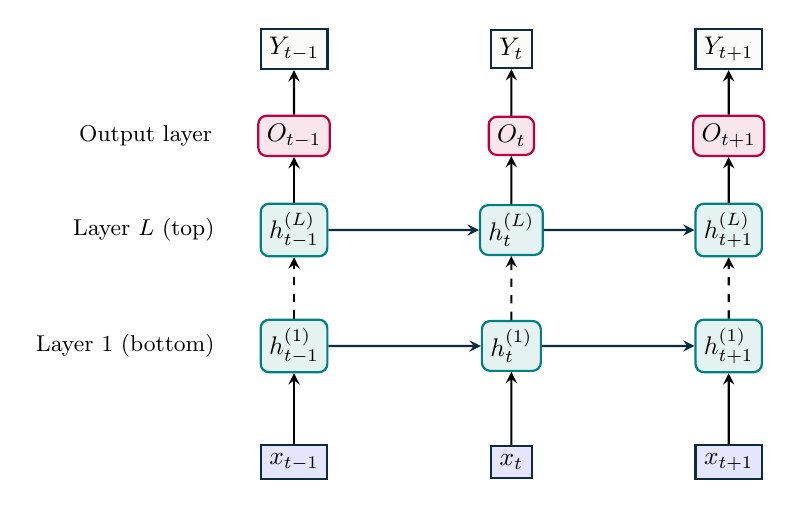
\begin{tikzpicture}[node distance=1.6cm, >=stealth, auto, scale=0.92, transform shape]
    % Output layer
    \node[rectangle, draw=purple, fill=purple!10, thick, rounded corners=3pt] (o1) at (0, 4.5) {$O_{t-1}$};
    \node[rectangle, draw=purple, fill=purple!10, thick, rounded corners=3pt] (o2) at (3, 4.5) {$O_t$};
    \node[rectangle, draw=purple, fill=purple!10, thick, rounded corners=3pt] (o3) at (6, 4.5) {$O_{t+1}$};
    
    \node[rectangle, draw=primaryblue, fill=lightbg, thick] (y1) at (0, 5.7) {$Y_{t-1}$};
    \node[rectangle, draw=primaryblue, fill=lightbg, thick] (y2) at (3, 5.7) {$Y_t$};
    \node[rectangle, draw=primaryblue, fill=lightbg, thick] (y3) at (6, 5.7) {$Y_{t+1}$};
    
    % Layer L (top layer)
    \node[rectangle, draw=teal, fill=teal!10, thick, rounded corners=3pt] (hL1) at (0, 3.2) {$h_{t-1}^{(L)}$};
    \node[rectangle, draw=teal, fill=teal!10, thick, rounded corners=3pt] (hL2) at (3, 3.2) {$h_t^{(L)}$};
    \node[rectangle, draw=teal, fill=teal!10, thick, rounded corners=3pt] (hL3) at (6, 3.2) {$h_{t+1}^{(L)}$};
    
    % Layer 1 (bottom layer)
    \node[rectangle, draw=teal, fill=teal!10, thick, rounded corners=3pt] (h11) at (0, 1.6) {$h_{t-1}^{(1)}$};
    \node[rectangle, draw=teal, fill=teal!10, thick, rounded corners=3pt] (h12) at (3, 1.6) {$h_t^{(1)}$};
    \node[rectangle, draw=teal, fill=teal!10, thick, rounded corners=3pt] (h13) at (6, 1.6) {$h_{t+1}^{(1)}$};
    
    % Input layer
    \node[rectangle, draw=primaryblue, fill=blue!10, thick] (x1) at (0, 0) {$x_{t-1}$};
    \node[rectangle, draw=primaryblue, fill=blue!10, thick] (x2) at (3, 0) {$x_t$};
    \node[rectangle, draw=primaryblue, fill=blue!10, thick] (x3) at (6, 0) {$x_{t+1}$};
    
    % Horizontal recurrent connections
    \draw[->, thick, primaryblue] (h11) -- (h12); \draw[->, thick, primaryblue] (h12) -- (h13);
    \draw[->, thick, primaryblue] (hL1) -- (hL2); \draw[->, thick, primaryblue] (hL2) -- (hL3);
    
    % Vertical connections between layers
    \draw[->, thick] (x1) -- (h11); \draw[->, thick] (x2) -- (h12); \draw[->, thick] (x3) -- (h13);
    \draw[->, thick, dashed] (h11) -- (hL1); \draw[->, thick, dashed] (h12) -- (hL2); \draw[->, thick, dashed] (h13) -- (hL3);
    \draw[->, thick] (hL1) -- (o1); \draw[->, thick] (hL2) -- (o2); \draw[->, thick] (hL3) -- (o3);
    \draw[->, thick] (o1) -- (y1); \draw[->, thick] (o2) -- (y2); \draw[->, thick] (o3) -- (y3);

    \node[left=0.5cm of h11] {\small Layer 1 (bottom)};
    \node[left=0.5cm of hL1] {\small Layer $L$ (top)};
    \node[left=0.5cm of o1] {\small Output layer};
\end{tikzpicture}
\caption{Stacked (Deep) Recurrent Neural Network Architecture.}
\label{fig:stacked_rnn_p81}
\end{figure}

Stacking recurrent layers increases the capacity of the per-step transformation while keeping temporal recursion at every level. This tends to help when the dataset is large enough to support more parameters without overfitting, a bias-variance trade-off that also applies to depth in any network.

Each layer has its own independent set of weights; nothing is shared across layers.

\textbf{Implementation:}
\begin{lstlisting}[language=Python]
model.add(LSTM(state_dim, return_sequences=True))
model.add(LSTM(state_dim, return_sequences=True))
model.add(LSTM(state_dim, return_sequences=True))
model.add(Dense(1, activation='sigmoid'))
\end{lstlisting}

\textbf{General Equation:}
\begin{equation}
h_t^{(l)} = f(W^{(l)} h_t^{(l-1)} + U^{(l)} h_{t-1}^{(l)} + b^{(l)})
\end{equation}

Stacked RNN are more prone to overfitting.
\textbf{Dropout randomly:} The Goal is to improve generalization without changing the architecture.

\section{Bidirectional Recurrent Neural Networks (Bi-RNN)}

\textbf{II) Bidirectional RNNs (Bi-RNN)}

\begin{figure}[htbp]
\centering
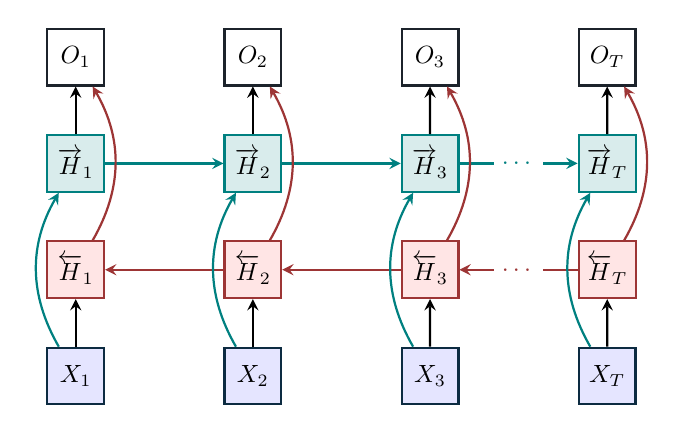
\begin{tikzpicture}[scale=0.9, transform shape, >=stealth]
    % Output Row
    \node[rectangle, draw=darkslate, fill=white, thick, minimum size=0.8cm] (o1) at (0, 4.5) {$O_1$};
    \node[rectangle, draw=darkslate, fill=white, thick, minimum size=0.8cm] (o2) at (2.5, 4.5) {$O_2$};
    \node[rectangle, draw=darkslate, fill=white, thick, minimum size=0.8cm] (o3) at (5.0, 4.5) {$O_3$};
    \node[rectangle, draw=darkslate, fill=white, thick, minimum size=0.8cm] (oT) at (7.5, 4.5) {$O_T$};
    
    % Forward Hidden Row (Green)
    \node[rectangle, draw=teal, fill=teal!15, thick, minimum size=0.8cm] (f1) at (0, 3.0) {$\overrightarrow{H}_1$};
    \node[rectangle, draw=teal, fill=teal!15, thick, minimum size=0.8cm] (f2) at (2.5, 3.0) {$\overrightarrow{H}_2$};
    \node[rectangle, draw=teal, fill=teal!15, thick, minimum size=0.8cm] (f3) at (5.0, 3.0) {$\overrightarrow{H}_3$};
    \node[rectangle, draw=teal, fill=teal!15, thick, minimum size=0.8cm] (fT) at (7.5, 3.0) {$\overrightarrow{H}_T$};
    
    % Backward Hidden Row (Red)
    \node[rectangle, draw=accentred, fill=red!10, thick, minimum size=0.8cm] (b1) at (0, 1.5) {$\overleftarrow{H}_1$};
    \node[rectangle, draw=accentred, fill=red!10, thick, minimum size=0.8cm] (b2) at (2.5, 1.5) {$\overleftarrow{H}_2$};
    \node[rectangle, draw=accentred, fill=red!10, thick, minimum size=0.8cm] (b3) at (5.0, 1.5) {$\overleftarrow{H}_3$};
    \node[rectangle, draw=accentred, fill=red!10, thick, minimum size=0.8cm] (bT) at (7.5, 1.5) {$\overleftarrow{H}_T$};
    
    % Input Row (Blue)
    \node[rectangle, draw=primaryblue, fill=blue!10, thick, minimum size=0.8cm] (x1) at (0, 0) {$X_1$};
    \node[rectangle, draw=primaryblue, fill=blue!10, thick, minimum size=0.8cm] (x2) at (2.5, 0) {$X_2$};
    \node[rectangle, draw=primaryblue, fill=blue!10, thick, minimum size=0.8cm] (x3) at (5.0, 0) {$X_3$};
    \node[rectangle, draw=primaryblue, fill=blue!10, thick, minimum size=0.8cm] (xT) at (7.5, 0) {$X_T$};
    
    % Forward Horizontal Connections (Green)
    \draw[->, thick, teal] (f1) -- (f2); \draw[->, thick, teal] (f2) -- (f3);
    \draw[->, thick, teal] (f3) -- node[midway, fill=white] {$\dots$} (fT);
    
    % Backward Horizontal Connections (Red)
    \draw[->, thick, accentred] (bT) -- node[midway, fill=white] {$\dots$} (b3);
    \draw[->, thick, accentred] (b3) -- (b2); \draw[->, thick, accentred] (b2) -- (b1);
    
    % Inputs to Hidden
    \draw[->, thick] (x1) -- (b1); \draw[->, thick] (x2) -- (b2); \draw[->, thick] (x3) -- (b3); \draw[->, thick] (xT) -- (bT);
    \draw[->, thick, teal, bend left=30] (x1) to (f1);
    \draw[->, thick, teal, bend left=30] (x2) to (f2);
    \draw[->, thick, teal, bend left=30] (x3) to (f3);
    \draw[->, thick, teal, bend left=30] (xT) to (fT);
    
    % Hidden to Output
    \draw[->, thick] (f1) -- (o1); \draw[->, thick] (f2) -- (o2); \draw[->, thick] (f3) -- (o3); \draw[->, thick] (fT) -- (oT);
    \draw[->, thick, accentred, bend right=30] (b1) to (o1);
    \draw[->, thick, accentred, bend right=30] (b2) to (o2);
    \draw[->, thick, accentred, bend right=30] (b3) to (o3);
    \draw[->, thick, accentred, bend right=30] (bT) to (oT);
\end{tikzpicture}
\caption{Bidirectional Recurrent Neural Network (Bi-RNN) Graph.}
\label{fig:birnn_p83}
\end{figure}

\textbf{Motivation:}
Many machine learning problems require understanding both past and Future context.

\begin{advbox}[Context Example]
\begin{align*}
\text{Example: } & \text{I deposited money in the bank} \to \text{Financial institution} \\
& \text{The Fisherman sat on the bank} \to \text{river Bank}
\end{align*}
So The: Previous words are insufficient. Future words are also important.
Understanding both left and Right Contexts improves interpretation.
\end{advbox}

Instead of One recurrent network we build two independent RNN:
\begin{itemize}
    \item \textbf{One Process:} Left $\to$ Right
    \item \textbf{The Second:} Left $\gets$ Right
\end{itemize}
Both networks analyze the same sentence independently. Finally, their outputs are merged.

\begin{align}
\text{Forward Hidden State: } & \overrightarrow{h}_t = \phi(W_f x_t + U_f \overrightarrow{h}_{t-1} + b_f) \\
\text{Backward Hidden State: } & \overleftarrow{h}_t = \phi(W_b x_t + U_b \overleftarrow{h}_{t+1} + b_b) \\
\text{The final Representation: } & h_t = [\overrightarrow{h}_t, \overleftarrow{h}_t]
\end{align}

\subsection{Bidirectional LSTM (Bi-LSTM)}

Instead of Using two Simple RNNs we Can Use two LSTM:
\begin{align}
\text{Forward LSTM compute: } & \overrightarrow{h}_t, \overrightarrow{C}_t \\
\text{Backward LSTM Compute: } & \overleftarrow{h}_t, \overleftarrow{C}_t \\
\text{Final output: } & h_t = [\overrightarrow{h}_t; \overleftarrow{h}_t]
\end{align}

Bi-LSTM combine the advantages of:
\begin{itemize}
    \item Long-term memory (LSTM)
    \item Future context (Bidirectional Processing)
\end{itemize}

\subsection{Limitations \& Practical Considerations}

\begin{advbox}[Limitation]
\begin{itemize}
    \item Approximately twice as many RNN parameters
    \item Increased GPU memory Consumption
    \item Long training and inference time
    \item Cannot be used for real time prediction because future inputs are Required.
\end{itemize}
\end{advbox}

\begin{propertybox}[Practical Consideration]
\begin{itemize}
    \item Use Simple RNN only For simple education examples
    \item Use LSTM when Long Term dependencies are important
    \item Use GRU when u need Similar Performance to an LSTM with fewer parameters and Faster training
    \item Use a Bidirectional LSTM when The entire Sequence is available before making a Prediction and Maximum Contextual understanding is Required.
\end{itemize}
\end{propertybox}

\section{Text Generation \& Encoder-Decoder Pipeline}

\textbf{Text Generation with RNN Steps:}

\begin{enumerate}
    \item \textbf{Text Cleaning:}
    \begin{itemize}
        \item Convert all letters to lowercase
        \item Remove unnecessary Symbols
        \item Remove extra Spaces
    \end{itemize}
    \item \textbf{Tokenization:} split text into words to characters
    \item \textbf{Word Indexing:} assign each unique word an integer ID
    \item \textbf{Text to Sequence:} replace words with their Corresponding indices
    \item \textbf{Padding / Truncation:} ensure all Sequences have the Same length for batch processing.
    \item \textbf{Word Embedding:} words are represented as dense vectors instead of one-hot vectors. An Embedding layer transform each word index into a Continuous vector that Captures Semantic relationships. This embedding layer often Contains the Largest number of Parameters in The model.
    \item \textbf{Passed Sentence into RNN Model} that's fast play The Role of Encoder: compressed The entire Sentence into one vector. This vector Summarizes the meaning of The input.
\end{enumerate}

So encoder Produce $h_T$ where $T = \text{last word of The Sentence}$, $h_T = \text{Final hidden State}$.
This hidden state called the: Context Vector OR Sentence Representation.

\begin{enumerate}[resume]
    \item \textbf{Bottleneck (Context Vector):} The encoder passes only one vector to The decoder. This vector is called:
    \begin{itemize}
        \item Context Vector
        \item Latent Vector
        \item Bottleneck
        \item Thought Vector
    \end{itemize}
    The bottleneck contains the information needed to reconstruct or Generate the output Sequence.
    \item \textbf{Decoder:} receives the context vector and Starts Generating the Output Sequence. The decoder Generate one token at time.
\end{enumerate}

\textbf{Decoder Process:}
\begin{enumerate}
    \item Receive the context Vector
    \item Generate one word
    \item Feed the Generated word back into The decoder
    \item Generate the next word
    \item Repeat until End-of-Sequence (EOS) token is produced
\end{enumerate}

\begin{advbox}[Limitation]
\begin{itemize}
    \item Fixed-size bottleneck can be lose information for long Sequence.
    \item Performance decreases as input length increase.
    \item This limitation is addressed by Attention, which allows the decoder to access all encoder hidden states instead of only the final context vector.
\end{itemize}
\end{advbox}

% ====================================================================
% Chapter 3 Continuation: Attention Mechanisms & Image Captioning
% (Digitized directly from Author Manuscript Pages 90 - 105)
% ====================================================================

\section{Attention Mechanism for Seq2Seq RNNs}

The first Seq2Seq (Encoder-Decoder) models solved the problem of mapping an input sequence to an output sequence; however, they suffered from a major limitation: the decoder relied only on a single fixed-size context vector (the bottleneck). For long sentences, this vector could not preserve all the information from the source sequence, causing translation and text generation quality to degrade. 

The \textbf{Attention Mechanism} was introduced to overcome this limitation by allowing the decoder to dynamically focus on the most relevant parts of the input sequence during each decoding step.

\subsection{Main Idea of Attention}

Instead of using only one context vector, the decoder can look at all encoder hidden states whenever it generates a new output word. Instead of $c = h_m$, we compute a different context vector for every decoder step.

So,
\begin{itemize}
    \item Encoder stores all hidden states.
    \item Decoder decides which hidden states are most useful.
    \item The decision is made through attention weights.
\end{itemize}

\begin{figure}[htbp]
\centering
\includegraphics[width=0.92\textwidth]{3-RNN/graph1_seq2seq.png}
\caption{Encoder-Decoder RNN (Seq2Seq) Architecture and Sequence-to-Sequence Performance comparison showing performance degradation without attention versus sustained quality with attention.}
\label{fig:seq2seq_attention_comparison}
\end{figure}

\subsection{Calculate Attention Step by Step}

\begin{itemize}
    \item \textbf{Without attention:} The final state is incapable of remembering a long sequence.
    \item \textbf{With attention:} Seq2Seq model does not forget source input and the decoder knows where to focus.
\end{itemize}

\begin{figure}[htbp]
\centering
\includegraphics[width=0.92\textwidth]{3-RNN/graph2_attention_step_by_step.png}
\caption{Step-by-Step Calculation of Attention: Encoder states $h_i$, Decoder state $S_{t-1}$, Linear Projections, Alignment Score $e_{ti}$, Softmax Attention Weight $\alpha_{ti}$, and Context Vector $c_t$.}
\label{fig:attention_step_by_step_diagram}
\end{figure}

This vector $c_t$ is a focused snapshot of the input sequence; it acts as a dynamic summary that changes for every word the decoder generates.

\textbf{Repeat for every output word:}
Attention is recomputed at every decoder time step:
\begin{enumerate}
    \item Compute alignment
    \item Compute attention weights
    \item Compute context vector $c_t$
\end{enumerate}

\begin{propertybox}[Numerical Example of Attention Weights]
Suppose alignment scores are $e_1 = 1, e_2 = 2, e_3 = 3$.
Applying Softmax normalization:
\begin{equation}
e_1 = \frac{2.7}{30}, \quad e_2 = \frac{7.3}{30}, \quad e_3 = \frac{20}{30}
\end{equation}
resulting in attention weights:
\begin{equation}
\alpha_1 = 0.09, \quad \alpha_2 = 0.20, \quad \alpha_3 = 0.665
\end{equation}
The context vector is computed as:
\begin{equation}
C = \alpha_1 h_1 + \alpha_2 h_2 + \alpha_3 h_3
\end{equation}
Here, state $h_3$ receives the highest weight ($\alpha_3 = 0.665$), receiving the most attention.
\end{propertybox}

\subsection{Advantages \& Limitations of Attention}

\begin{advbox}[Advantages]
\begin{itemize}
    \item Eliminates the fixed-size bottleneck.
    \item Handles long input sequences much better.
    \item Produces better translations and generated text.
    \item Learns where to focus automatically.
    \item Generates a different context vector for each output word.
    \item Greatly improves Seq2Seq performance.
\end{itemize}
\end{advbox}

\begin{advbox}[Limitations]
\begin{itemize}
    \item Higher computational cost.
    \item Increased memory usage.
    \item Attention weights must be recomputed for every decoder step.
    \item Complexity grows with both input and output sequence lengths.
\end{itemize}
\end{advbox}

\begin{propertybox}[Summary of Attention Mechanism]
The Attention Mechanism enhances the classical Encoder-Decoder architecture by allowing the decoder to access all encoder hidden states instead of relying on a single bottleneck vector. At each decoding step, the decoder computes alignment scores, converts them into attention weights using Softmax, forms a context vector as a weighted sum of the encoder hidden states, and uses this context to generate the next output token. Because a new context vector is computed for every output step, the model learns where to focus in the input sequence, greatly improving performance on long sequences at the cost of increased computational complexity.
\end{propertybox}

\section{Self-Attention in RNN}

\textbf{Self-Attention in RNN} is a neural mechanism that enables a model to determine which parts of its own input sequence are the most relevant when computing the representation of the current element. Instead of relying only on the previous hidden state, the model compares the current hidden state with all previous hidden states and selectively focuses on the most informative ones.

In RNNs, self-attention improves the network's ability to model long-range dependencies by allowing it to retrieve information from any previous time step.

\begin{itemize}
    \item \textbf{In Attention:} The decoder looks at the encoder's hidden states.
    \item \textbf{In Self-Attention:} The model looks at previous decoder hidden states, meaning the decoder is attending to its own previous hidden states, in addition to (or instead of) attending to the encoder.
\end{itemize}

\textbf{Decoder Self-Attention:} \textit{"Which words have I already generated that are important for predicting the next word?"}

\textit{Example:} \textit{"Mohamed likes studying at night"} (where \textit{studying} attends back to \textit{Mohamed}).

\begin{figure}[htbp]
\centering
\includegraphics[width=0.88\textwidth]{3-RNN/graph3_decoder.png}
\caption{Decoder architecture integrating self-attention context vectors $C_1, C_2, C_3, C_4$ across hidden states $h_1, h_2, h_3, h_4$.}
\label{fig:decoder_self_attention_graph}
\end{figure}

The updated state and context vectors are formulated as:
\begin{equation}
h_4 = \tanh\left(A \cdot \begin{bmatrix} x_4 \\ C_3 \end{bmatrix} + b\right)
\end{equation}
\begin{equation}
\text{weights: } \alpha_i = \operatorname{align}(h_i, h_4)
\end{equation}
\begin{equation}
C_4 = \alpha_1 h_1 + \alpha_2 h_2 + \alpha_3 h_3 + \alpha_4 h_4 \quad \text{(repeated for every new generated word)}
\end{equation}

\begin{propertybox}[Historical Literature References]
\textbf{Notice:} The original self-attention paper uses LSTM networks. Two foundational papers reference Attention and Self-Attention:
\begin{enumerate}
    \item \textbf{Bahdanau, Cho \& Bengio (2015):} Encoder-Decoder Attention ($\text{Query} = \text{decoder state}$, $\text{Keys}/\text{Values} = \text{encoder states}$ across two different sequences).
    \item \textbf{Cheng, Dong \& Lapata (2016):} \textit{"Long Short-Term Memory Network for Machine Reading"}, where the Query, Keys, and Values all come from the same sequence (a single RNN attending to its own history). This is the direct conceptual ancestor of Transformer self-attention.
\end{enumerate}
\end{propertybox}

\subsection{Self-Attention Mechanism Step-by-Step}

\begin{align}
\tilde{h}_t &= \tanh(A[h_{t-1}, x_t] + b) \\
e_i &= \operatorname{align}(\tilde{h}_t, h_i) \quad \text{for } i = 1, \dots, t \\
e_i &= v^T \tanh(W_1 \tilde{h}_t + W_2 h_i) \\
\alpha_i &= \operatorname{softmax}(e_i) \\
c_t &= \sum_{i=1}^t \alpha_i h_i \quad \text{(context vector, repeat until EOS)}
\end{align}

\begin{advbox}[Advantages of Self-Attention in RNNs]
\begin{itemize}
    \item Reduces forgetting of long-term information.
    \item Allows direct access to earlier hidden states.
    \item Learns automatically where to focus.
    \item Improves the representation of long sequences.
    \item Serves as a bridge between classical RNNs and modern Transformer architectures.
\end{itemize}
\end{advbox}

\begin{advbox}[Limitations of Self-Attention in RNNs]
\begin{itemize}
    \item Computational complexity increases because attention must be computed at every time step.
    \item All hidden states must be stored in memory.
    \item Still processes the sequence sequentially, unlike Transformers which compute self-attention in parallel.
\end{itemize}
\end{advbox}

\section{Image Caption Generation Architecture (CNN-LSTM Model)}

\textbf{Project: Image Caption Generation using CNN and LSTM}

Image Captioning is the task of automatically generating a natural language description for an image. Image captioning combines two major fields:
\begin{itemize}
    \item \textbf{Computer Vision:} to understand the content of the image.
    \item \textbf{Natural Language Processing (NLP):} to generate the describing sentence.
\end{itemize}

\begin{figure}[htbp]
\centering
\includegraphics[width=0.92\textwidth]{3-RNN/graph4_image_captioning.png}
\caption{Complete Image Caption Generation Multimodal System Architecture.}
\label{fig:image_captioning_architecture_multimodal}
\end{figure}

\begin{propertybox}[Dataset: Flickr8K]
\textbf{Characteristics:}
\begin{itemize}
    \item Approximately $8,000$ images.
    \item Every image has $5$ different captions ($30,000$ total captions).
    \item Around $6,000$ images are used for training.
\end{itemize}
\end{propertybox}

\subsection{Pipeline Steps}

\begin{enumerate}
    \item \textbf{Step 1: Feature Extraction (Transfer Learning)} \\
    Instead of training a CNN from scratch (which requires millions of images), the project uses a pretrained VGG16 network via Transfer Learning. The process reuses a model that has already learned rich visual representations from ImageNet.
    
    The final classification layer in VGG16 is removed, leaving a $4096$-dimensional feature vector that summarizes the visual content of the image.

    \item \textbf{Step 2: Captions Processing} \\
    Captions undergo preprocessing:
    \begin{itemize}
        \item Add Special Tokens: \texttt{startseq A child in a pink dress endseq} to indicate start and end boundaries.
        \item Tokenization: \texttt{['startseq', 'A', 'child', 'in', 'a', 'pink', 'dress', 'endseq']}
        \item Integer Encoding: \texttt{startseq} $\to 2$, \texttt{a} $\to 1$, \texttt{child} $\to 43$, \texttt{pink} $\to 90$, \texttt{dress} $\to 172$, \dots, \texttt{endseq} $\to 3$. The caption becomes $[2, 1, 43, 90, 172, \dots, 3]$.
    \end{itemize}

    \item \textbf{Step 3: Create Training Samples} \\
    The network learns next-word prediction:
    \begin{table}[htbp]
    \centering
    \begin{tabular}{l | l}
    \hline
    \textbf{Input (Partial Caption)} & \textbf{Target (Next Word)} \\
    \hline
    \texttt{startseq} & \texttt{a} \\
    \texttt{startseq a} & \texttt{cat} \\
    \texttt{startseq a cat} & \texttt{sat} \\
    \texttt{startseq a cat sat} & \texttt{on} \\
    \vdots & \vdots \\
    \hline
    \end{tabular}
    \caption{Training samples pair partial sequence input to next target word. Each sample includes the same image feature vector from VGG16.}
    \end{table}

    \item \textbf{Step 4: Padding Sequences} \\
    Sequences have different lengths. To create mini-batches, they are padded with zero tokens to the maximum sentence length, e.g.:
    \begin{equation}
    [\text{Hi}, \text{how}, \text{are}, \text{you}, \langle \text{Pad} \rangle, \langle \text{Pad} \rangle, \langle \text{Pad} \rangle] \implies [2, 1, 43, 50, 0, 0, 0]
    \end{equation}

    \item \textbf{Step 5: One-Hot Encoding} \\
    The target word is converted into a One-Hot vector over the vocabulary.

    \item \textbf{Step 6: Build the Neural Network Architecture} \\
    The dual-branch architecture connects as follows:
    \begin{itemize}
        \item \textbf{Image Branch:} Raw Image $\to$ VGG16 Features ($4096$) $\to$ Dropout $\to$ Dense ($256$).
        \item \textbf{Text Branch:} Previous Words $\to$ Embedding Layer $\to$ LSTM Network ($256$).
    \end{itemize}
    The outputs of the two branches ($256$ dimensions each) are then added (or concatenated), followed by additional dense layers and a final Softmax layer over the vocabulary.

    \item \textbf{Step 7: Training} \\
    Each training sample consists of $(x_1, x_2, y)$, where $x_1$ is the image feature vector, $x_2$ is the partial caption sequence, and $y$ is the target next word. The network minimizes Categorical Cross-Entropy loss.
\end{enumerate}

\subsection{Caption Generation (Inference Pipeline)}

\begin{enumerate}
    \item Input an unlabelled image.
    \item Extract its feature vector using VGG16.
    \item Initialize the caption sequence with \texttt{startseq}.
    \item Feed the image features and current partial caption into the network.
    \item Predict the probability distribution over the next word.
    \item Append the predicted word to the caption.
    \item Repeat steps 4--6 until \texttt{endseq} is predicted or maximum caption length is reached.
\end{enumerate}

\begin{propertybox}[Modern Perspective]
\textbf{Notice:} Modern captioning systems often replace LSTMs with Transformers and add visual attention mechanisms to dynamically focus on specific spatial image regions during decoding.
\end{propertybox}



% ====================================================================
% Chapter 4: Transfer Learning
% (Digitized directly from Author Manuscript Pages 106 - 117)
% ====================================================================

\chapter{Transfer Learning}

A.I. systems learn by extracting patterns from data. In traditional machine learning and deep learning, every new task is usually learned from scratch. This means that whenever a new problem arises, the model begins with randomly initialized parameters and must learn everything again, even if it has previously solved similar problems.

\begin{propertybox}[Definition: Transfer Learning]
\textbf{Transfer Learning} is the process of improving learning in a target task by reusing knowledge acquired from a previously learned source task.
\end{propertybox}

\section{Why Is Transfer Learning Needed?}

Early deep learning systems faced three major challenges:

\subsection{Data Scarcity}
Deep neural networks contain millions or even billions of trainable parameters. For example:
\begin{itemize}
    \item \textbf{LeNet:} $60,000$ parameters
    \item \textbf{AlexNet:} $60$ million parameters
    \item \textbf{ResNet:} $25$ million parameters
    \item \textbf{GPT-3:} $175$ billion parameters
\end{itemize}
Training such models requires enormous datasets.

\subsection{Computational Cost}
Training a deep neural network from random initialization is computationally expensive. Training large models may require:
\begin{itemize}
    \item Multiple GPUs / TPUs
    \item Days or weeks of computation
    \item Large electrical power consumption
\end{itemize}
Transfer Learning significantly reduces these costs because much of the learning has already been completed during pretraining.

\subsection{Training Time}
Training time often decreases from weeks $\to$ days $\to$ hours $\to$ sometimes only minutes!

\begin{propertybox}[Human Analogy of Transfer Learning]
Transfer Learning behaves like human learning and can be viewed as:
\begin{equation}
\text{Knowledge}_{\text{new}} = \text{Knowledge}_{\text{previous}} + \text{New Experience}
\end{equation}
Transfer Learning attempts to reproduce this behavior in artificial neural networks.
\end{propertybox}

\section{Types of Transfer Learning}

Transfer Learning is classified according to whether the source and target tasks/domains are the same or different.

\subsection{Inductive Transfer Learning}
The target task is different from the source task, regardless of whether the domains are the same or different ($T_S \neq T_T$).
\begin{itemize}
    \item \textbf{Source:} ImageNet $\to$ Image Classification
    \item \textbf{Target:} Medical Image Classification
\end{itemize}
Although both involve images, the classification tasks are different.

\subsection{Transductive Transfer Learning (Domain Adaptation)}
The task remains the same, but the data distribution (domain) changes ($D_S \neq D_T, T_S = T_T$).
\begin{itemize}
    \item \textbf{Trains on:} Daytime street images
    \item \textbf{Test on:} Nighttime street images
\end{itemize}
The task (object detection) is identical, but the image distributions differ.

\subsection{Unsupervised Transfer Learning}
Both the source and target tasks are unsupervised, meaning there are no labels. Typical tasks include:
\begin{itemize}
    \item Clustering
    \item Dimensionality Reduction
    \item Representation Learning
\end{itemize}
\textit{Example:} A self-supervised model trained on millions of unlabeled images is transferred to another unlabeled image dataset.

\section{Transfer Dynamics: Positive vs. Negative Transfer}

\begin{advbox}[Positive Transfer]
Knowledge learned from the source task improves performance on the target task:
\begin{equation}
\text{Accuracy}_{\text{Transfer}} > \text{Accuracy}_{\text{scratch}}
\end{equation}
\textit{Example:} ImageNet $\to$ Medical X-ray. The pretrained CNN already knows edges, textures, and shapes, allowing faster learning and higher accuracy.
\end{advbox}

\begin{advbox}[Negative Transfer]
Transferred knowledge actually reduces performance:
\begin{equation}
\text{Accuracy}_{\text{Transfer}} < \text{Accuracy}_{\text{scratch}}
\end{equation}
\textit{Example:} A CNN trained on satellite images is transferred to handwritten digit recognition. The learned features are largely unrelated, so the transferred knowledge may hurt performance.
\end{advbox}

\subsection{When Transfer Learning Works Well}
Transfer Learning works well when:
\begin{itemize}
    \item Source and target domains are similar.
    \item The pretrained model learned general features.
    \item The target dataset is small.
    \item The source dataset is large and diverse.
    \item The target task is related to the source task.
\end{itemize}

\textbf{Common Examples:}
\begin{itemize}
    \item ImageNet $\to$ Medical Images
    \item ImageNet $\to$ Plant Disease Detection
    \item BERT $\to$ Sentiment Analysis
    \item GPT $\to$ Question Answering
\end{itemize}

\subsection{When Transfer Learning May Fail}
Transfer Learning may fail when:
\begin{itemize}
    \item Source and target domains are very different.
    \item The pretrained features are not useful.
    \item The source model contains strong biases.
    \item The target dataset is extremely different.
    \item Too much fine-tuning causes catastrophic forgetting.
\end{itemize}

\section{Application Strategies: Feature Extraction vs. Fine-Tuning}

Transfer Learning can be applied in two main ways:

\subsection{Feature Extraction}
Uses the pretrained model as a fixed feature extractor. The pretrained layers are frozen, meaning their weights remain unchanged during training. Only a new output layer (classifier) is added and trained on the target dataset (we just replace the last layer of the network).

\textbf{Characteristics:}
\begin{itemize}
    \item Pretrained weights are frozen.
    \item Only the new classifier learns.
    \item Very fast training.
    \item Requires a small dataset.
    \item Low risk of overfitting.
\end{itemize}

\subsection{Fine-Tuning}
Fine-Tuning starts with a pretrained model but allows some or all of the pretrained weights to continue learning. Instead of freezing every layer, selected layers are unfrozen and updated using the new dataset.

\textbf{Characteristics:}
\begin{itemize}
    \item Some or all pretrained layers are trainable.
    \item The classifier is always replaced and trained.
    \item Produces better adaptation to the target task.
    \item Requires more data.
    \item Higher computational cost.
    \item Greater risk of overfitting if the dataset is too small.
\end{itemize}

\begin{propertybox}[Do We Change the Input Layer in Transfer Learning?]
\textbf{Usually no.} The input layer is kept because the pretrained model expects a specific input size:
\begin{itemize}
    \item \textbf{VGG16:} $224 \times 224 \times 3$
    \item \textbf{ResNet50:} $224 \times 224 \times 3$
    \item \textbf{EfficientNetB0:} $224 \times 224 \times 3$
\end{itemize}
If our images have a different size, we usually resize the images, not the network.
\end{propertybox}

\section{Advanced Fine-Tuning Techniques}

\subsection{Partial Fine-Tuning}
Instead of training the entire network, only the last few layers are unfrozen while the earlier layers remain frozen. This is the most commonly used fine-tuning strategy because early layers learn generic features while deeper layers learn task-specific representations.

\subsection{Progressive Unfreezing}
Instead of unfreezing many layers at once, layers are unfrozen gradually:
\begin{enumerate}
    \item Classifier (last layer)
    \item Classifier + Last block
    \item Classifier + Last two blocks
    \item Classifier + Entire Network
\end{enumerate}
This provides more stable training and reduces catastrophic forgetting.

\subsection{Differential Learning Rates}
Different layers receive different learning rates. Early layers receive very small updates because they already contain useful general features, while newly added layers receive larger updates.

\begin{table}[htbp]
\centering
\begin{tabular}{l | l}
\hline
\textbf{Layer} & \textbf{Learning Rate} \\
\hline
Early layers & $1 \times 10^{-5}$ \\
Middle layers & $1 \times 10^{-5}$ \\
Last layers & $1 \times 10^{-4}$ \\
New Classifier & $1 \times 10^{-3}$ \\
\hline
\end{tabular}
\caption{Differential Learning Rates assigned per network layer depth.}
\end{table}

\section{Catastrophic Forgetting \& Regularization}

\textbf{Catastrophic Forgetting} occurs when fine-tuning causes the pretrained model to lose previously learned useful knowledge.

\begin{itemize}
    \item \textbf{Common Causes:} High learning rate, very small dataset, or training all layers immediately.
    \item \textbf{Solutions:} Freeze early layers, use small learning rates, apply progressive unfreezing, and use regularization.
\end{itemize}

\subsection{Regularization Techniques}
Regularization includes techniques that reduce overfitting by preventing the model from becoming too specialized on the training data. Common methods include Dropout, Weight Decay, Early Stopping, Data Augmentation, and Label Smoothing. The objective is to improve generalization on unseen data.

\begin{itemize}
    \item \textbf{Weight Decay ($L_2$ Regularization):} Penalizes large weights by adding a regularization term to the loss function:
    \begin{equation}
    L_{\text{total}} = L_{\text{task}} + \lambda \sum_i w_i^2
    \end{equation}
    
    \item \textbf{Early Stopping:} Instead of training for a fixed number of epochs, training ends once improvement has stalled for a predefined number of epochs (called patience).
    \begin{itemize}
        \item Prevents overfitting.
        \item Saves training time.
        \item Keeps the best-performing model.
    \end{itemize}
\end{itemize}

\subsection{Batch Normalization Issues}
During fine-tuning on small datasets, updating Batch Normalization statistics (mean and variance) can make training unstable. A common practice is:
\begin{itemize}
    \item Freeze BatchNorm layers when the target dataset is small.
    \item Update them only if sufficient data is available.
\end{itemize}

\section{Practical Recipes}

\begin{propertybox}[Scenario 1: Very Small Dataset (< 1000 images)]
\begin{itemize}
    \item Freeze the backbone.
    \item Train only the new classifier.
    \item Small learning rate.
    \item Use data augmentation.
\end{itemize}
\end{propertybox}

\begin{propertybox}[Scenario 2: Medium Dataset (1000 to 10000 images)]
\begin{itemize}
    \item Train the new classifier.
    \item Fine-tune the last few blocks.
    \item Use differential learning rates.
    \item Apply weight decay and early stopping.
\end{itemize}
\end{propertybox}

\begin{propertybox}[Scenario 3: Large Dataset (> 10000 to 50000 images)]
\begin{itemize}
    \item Fine-tune most or all layers.
    \item Use progressive unfreezing if needed.
    \item Tune learning rates carefully.
    \item Monitor validation performance to avoid overfitting.
\end{itemize}
\end{propertybox}

\chapter{Transformers}

\section{Motivation and Background}
Before 2017, almost every model for sequence processing relied on recurrent neural network (RNN) architectures. The standard sequence-to-sequence structure used an encoder RNN to process the input and compress it into a fixed-length context vector, which was then passed to a decoder:

\begin{center}
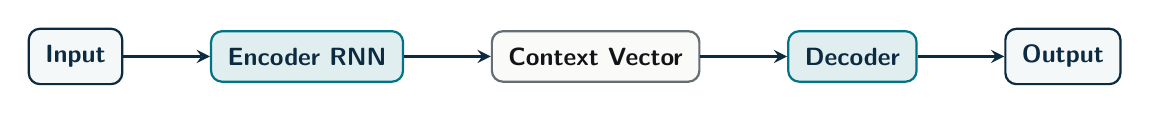
\begin{tikzpicture}[
    node distance=1.1cm, 
    auto, 
    >=stealth, 
    font=\sffamily\bfseries\small,
    mainnode/.style={draw=primaryblue, fill=boxbg, text=primaryblue, rounded corners=4pt, inner sep=6pt, line width=0.8pt},
    secnode/.style={draw=secondaryblue, fill=secondaryblue!12, text=primaryblue, rounded corners=4pt, inner sep=6pt, line width=0.8pt},
    graynode/.style={draw=warmgray, fill=lightbg, text=ink, rounded corners=4pt, inner sep=6pt, line width=0.8pt}
]
    \node [mainnode] (input1) {Input};
    \node [secnode, right=of input1] (enc1) {Encoder RNN};
    \node [graynode, right=of enc1] (ctx) {Context Vector};
    \node [secnode, right=of ctx] (dec1) {Decoder};
    \node [mainnode, right=of dec1] (out1) {Output};
    
    \draw [->, line width=1.1pt, primaryblue] (input1) -- (enc1);
    \draw [->, line width=1.1pt, primaryblue] (enc1) -- (ctx);
    \draw [->, line width=1.1pt, primaryblue] (ctx) -- (dec1);
    \draw [->, line width=1.1pt, primaryblue] (dec1) -- (out1);
\end{tikzpicture}
\end{center}

Later, attention mechanisms were introduced to connect the encoder and decoder directly:

\begin{center}
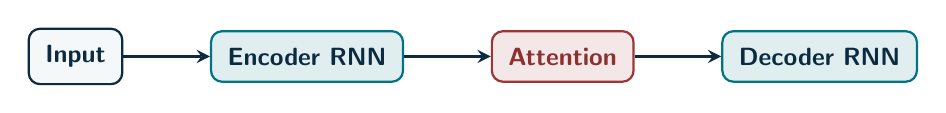
\begin{tikzpicture}[
    node distance=1.1cm, 
    auto, 
    >=stealth, 
    font=\sffamily\bfseries\small,
    mainnode/.style={draw=primaryblue, fill=boxbg, text=primaryblue, rounded corners=4pt, inner sep=6pt, line width=0.8pt},
    secnode/.style={draw=secondaryblue, fill=secondaryblue!12, text=primaryblue, rounded corners=4pt, inner sep=6pt, line width=0.8pt},
    attnode/.style={draw=accentred, fill=accentred!12, text=accentred!90!black, rounded corners=4pt, inner sep=6pt, line width=0.8pt}
]
    \node [mainnode] (input2) {Input};
    \node [secnode, right=of input2] (enc2) {Encoder RNN};
    \node [attnode, right=of enc2] (attn) {Attention};
    \node [secnode, right=of attn] (dec2) {Decoder RNN};
    
    \draw [->, line width=1.1pt, primaryblue] (input2) -- (enc2);
    \draw [->, line width=1.1pt, primaryblue] (enc2) -- (attn);
    \draw [->, line width=1.1pt, primaryblue] (attn) -- (dec2);
\end{tikzpicture}
\end{center}

Attention solved one major problem: the encoder no longer compresses the whole sentence into a single vector. Instead, the decoder could look back at all encoder hidden states. However, another huge problem remained.

\subsection{Limitations of Recurrent Architectures}
\textbf{Problem 1: Sequential Computation} \\
Each hidden state depends sequentially on the previous one:
\begin{equation}
h_t = f(h_{t-1}, x_t)
\end{equation}
This destroys parallelism. GPU utilization becomes poor, and training becomes exceptionally slow.

\textbf{Problem 2: Long Dependency} \\
Consider the sentence: \textit{“The animal didn't cross the street because \textbf{it} was too tired”}. \\
To understand “\textbf{it}”, the model must remember “animal” from dozens of words ago. Although LSTMs can model longer dependencies than vanilla RNNs, learning very long-range dependencies can still be challenging. Although attention helps, the underlying computation remains strictly sequential.

\textbf{Problem 3: Information Bottleneck} \\
Even with attention, the encoder still has to build hidden states sequentially. Earlier mistakes propagate forward, later words depend on previous computations, and errors accumulate across layers.

\section{Attention and Self-Attention}
This led to a fundamental question: \textit{Do we really need recurrent neural networks?} \\
The answer was to remove recurrence from the sequence-processing architecture while retaining attention. This allows the tokens of an input sequence to be processed in parallel during training:
\begin{equation*}
\text{input Embeddings} \longrightarrow \text{Self-Attention} \longrightarrow \text{Feed Forward}
\end{equation*}

How to remove RNN while keeping attention?

\subsection{Attention Without RNN}
Encoder's input: $[x_1, x_2, x_3, \dots, x_m]$ \\
Decoder's input: $[x_1', x_2', x_3', \dots, x_t']$ \\
Keys and values are based on encoder's inputs $x_1, x_2, \dots, x_m$.

\begin{figure}[htbp]
    \centering
    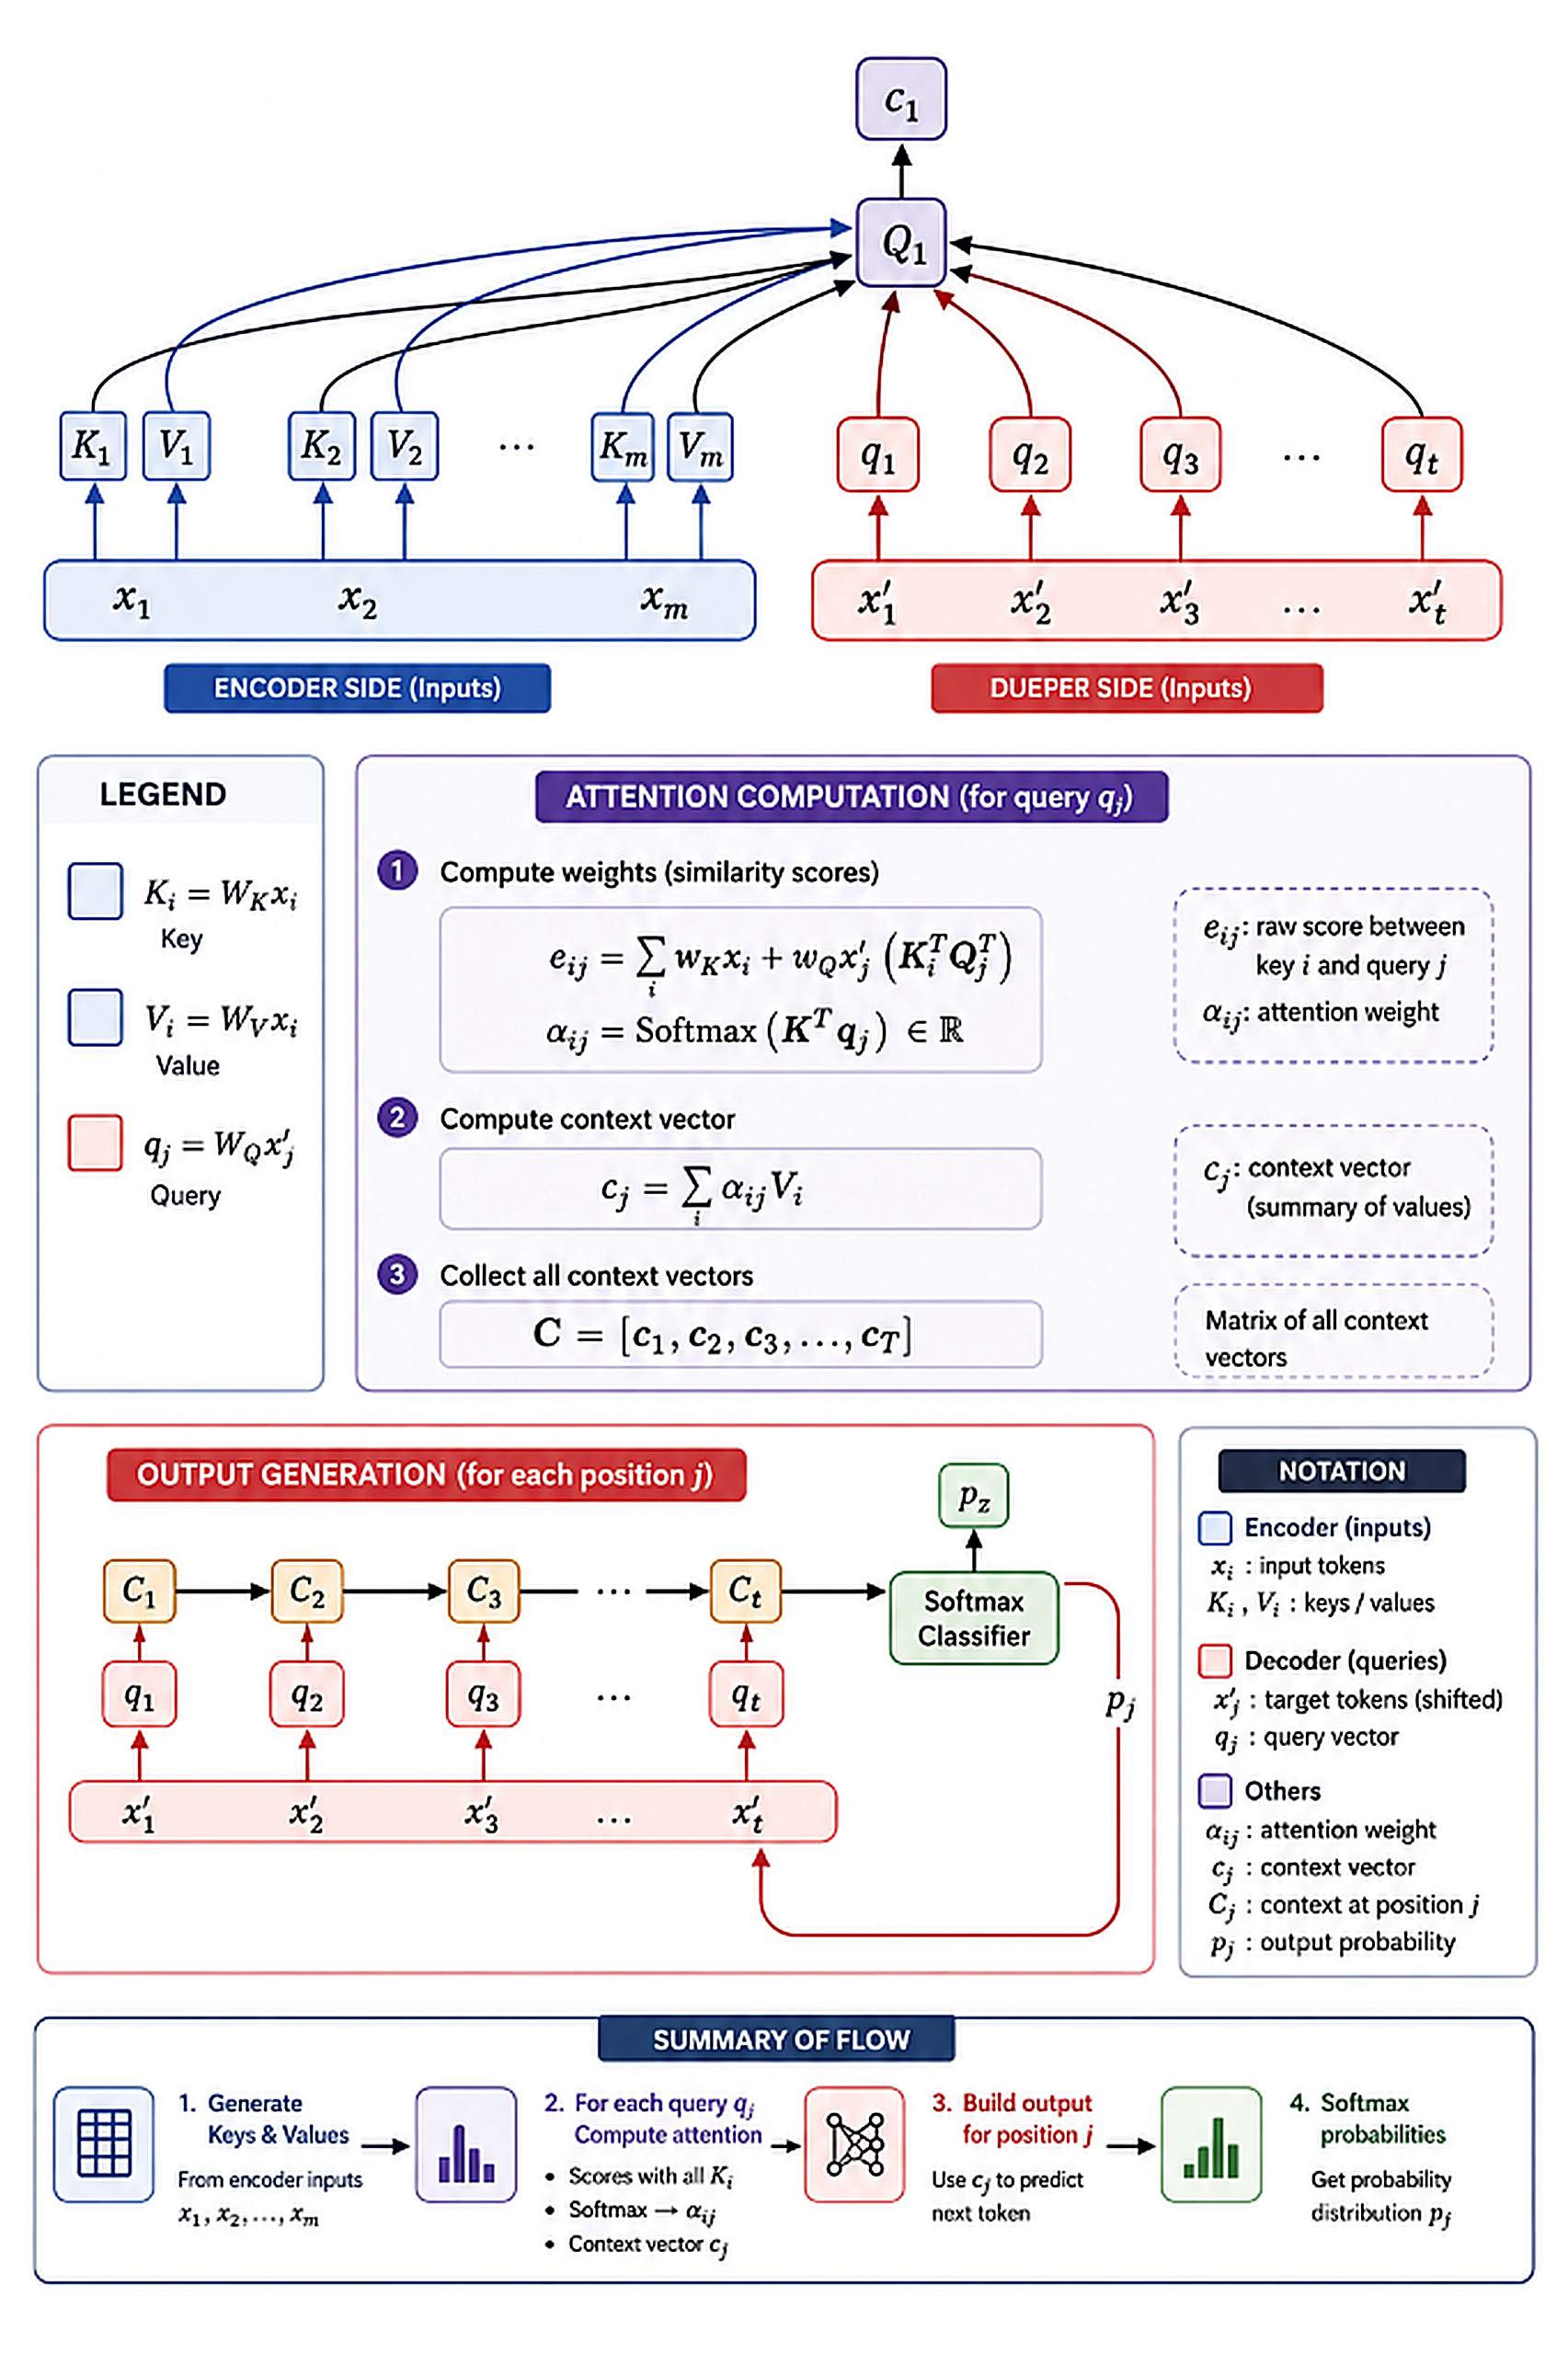
\includegraphics[width=0.85\textwidth]{figures/fig_5_attention_flow_pg121.png}
    \caption{Detailed computation flow of attention mechanisms operating over encoder and decoder inputs.}
    \label{fig:attention_flow_pg121}
\end{figure}

Key: $K_i = W_K x_i$ \\
Value: $V_i = W_V x_i$ \\
Query: $q_j = W_Q x_j'$

Compute weights:
\begin{equation}
\alpha_{ij} = \operatorname{softmax}_i\left(\frac{q_j K_i^T}{\sqrt{d_k}}\right)
\end{equation}

Compute Context Vector:
\begin{equation}
c_j = \sum_i \alpha_{ij} V_i, \quad C = [c_1, c_2, c_3, \dots, c_T]
\end{equation}

So Attention Layer: $C = \text{Attn}(x, x')$
\begin{itemize}
    \item Encoder inputs: $[x_1, x_2, x_3, \dots, x_m]$
    \item Decoder inputs: $[x_1', x_2', x_3', \dots, x_t']$
    \item Parameters: $W_Q, W_K, W_V$
\end{itemize}

Classical attention asks: \textit{Which encoder hidden states are important for this decoder state?} \\
Instead of directly comparing $h_i$ and $s_i$, we first project them into another space:
\begin{align}
q_t &= W_Q \cdot s_t \quad \text{(Query, obtained from decoder)} \\
K_i &= W_K \cdot h_i \quad \text{(Key, obtained from encoder)} \\
V_i &= W_V \cdot h_i \quad \text{(Value, obtained from encoder)}
\end{align}

\subsection{Why Do We Need \texorpdfstring{$Q, K, and V$}{Q, K, and V}?}
Why not compare with $h_i$ directly? Because different tasks need different notions of similarity. \\
For example, suppose “apple” sometimes means fruit, sometimes company.
\begin{itemize}
    \item The model learns $W_K$ to encode meaning.
    \item The model learns $W_Q$ to encode what we are looking for.
    \item The model learns $W_V$ to encode the information we finally want.
\end{itemize}

So Old Attention: Keys come from Encoder, Queries come from Decoder. \\
So let's come to the brilliant insight: \textit{Where do Queries really come from? Why not create them directly from the input?}

Instead of $q = W_Q s_i$, let's do:
\begin{align}
q &= W_Q x_i \quad \text{in the encoder} \\
K &= W_K x_i \\
V &= W_V x_i
\end{align}

Now: everything comes from the input itself:
\begin{itemize}
    \item No decoder state needed
    \item No encoder state needed
    \item Only embeddings
\end{itemize}

So that's what we call: \textbf{Self-Attention}.

In Self-Attention Layer: $C = \text{Attn}(X, X)$ \\
Input: $[x_1, x_2, \dots, x_m]$ \\
Parameters: $W_Q, W_K, W_V$

\begin{equation}
\alpha_i = \text{Softmax}(K^T q_i) \in \mathbb{R}^m
\end{equation}
\begin{equation}
c_i = V \cdot \alpha_i
\end{equation}
Output of Self-Attention layer: $[c_1, c_2, \dots, c_m]$.

This is the heart of the Transformer: Each word asks: \textit{Which other words help me understand myself?} \\
Example: “The animal didn't cross the street because it was tired”. \\
Token “it” creates Query and compares itself with every Key (e.g. animal: 0.8, street: 0.1 \dots). Output becomes mostly animal. This is exactly what Self-Attention computes.

\subsection{Mathematical Derivations}
Let $X = \begin{bmatrix} x_1 \\ x_2 \\ x_3 \\ \vdots \\ x_n \end{bmatrix}$. Project:
\begin{equation}
Q = X W_Q, \quad K = X W_K, \quad V = X W_V
\end{equation}
Similarity matrix: $S = Q K^T$ \\
Normalize: $A = \text{Softmax}(S)$ \\
Output: $C = A \cdot V$

The Full Equation:
\begin{equation}
\text{Attn}(Q, K, V) = \text{softmax}\left(\frac{Q K^T}{\sqrt{d_k}}\right) V
\end{equation}

Summary:
\begin{itemize}
    \item Classical attention lets a decoder query encoder representations.
    \item By generating Queries, Keys, and Values directly from the input embedding, we eliminate the need for recurrent hidden states.
    \item This leads to self-attention, where every token can attend to every other token in parallel.
    \item Self-attention becomes the fundamental building block of the Transformer.
    \item (Attention was originally developed for Seq2Seq RNN models, and self-attention for all RNN models, not necessarily Seq2Seq models).
\end{itemize}

\section{The "Attention Is All You Need" Paper Architecture}
The “Attention Is All You Need” paper, published by Vaswani et al. in 2017, introduced the Transformer, a novel neural network architecture that fundamentally changed sequence modeling. Unlike Seq2Seq models based on RNNs, LSTMs, and GRUs, the Transformer completely eliminates recurrence and relies solely on attention mechanisms to model dependencies between tokens. This design enables full parallel computation during training, significantly improves the modeling of long-range dependencies, and achieves superior computational efficiency.

The Transformer is built upon several key innovations, including Scaled Dot-Product Attention, Multi-Head Attention, Positional Encoding, Residual Connections, Layer Normalization, and Position-wise Feed-Forward Networks. These components are organized into an encoder-decoder architecture composed of stacked layers that learn increasingly rich contextual representations.

The Transformer has become the foundation of nearly all modern deep learning models for language, vision, speech, and multimodal learning: BERT, GPT, ViT, and LLMs.

\begin{figure}[htbp]
    \centering
    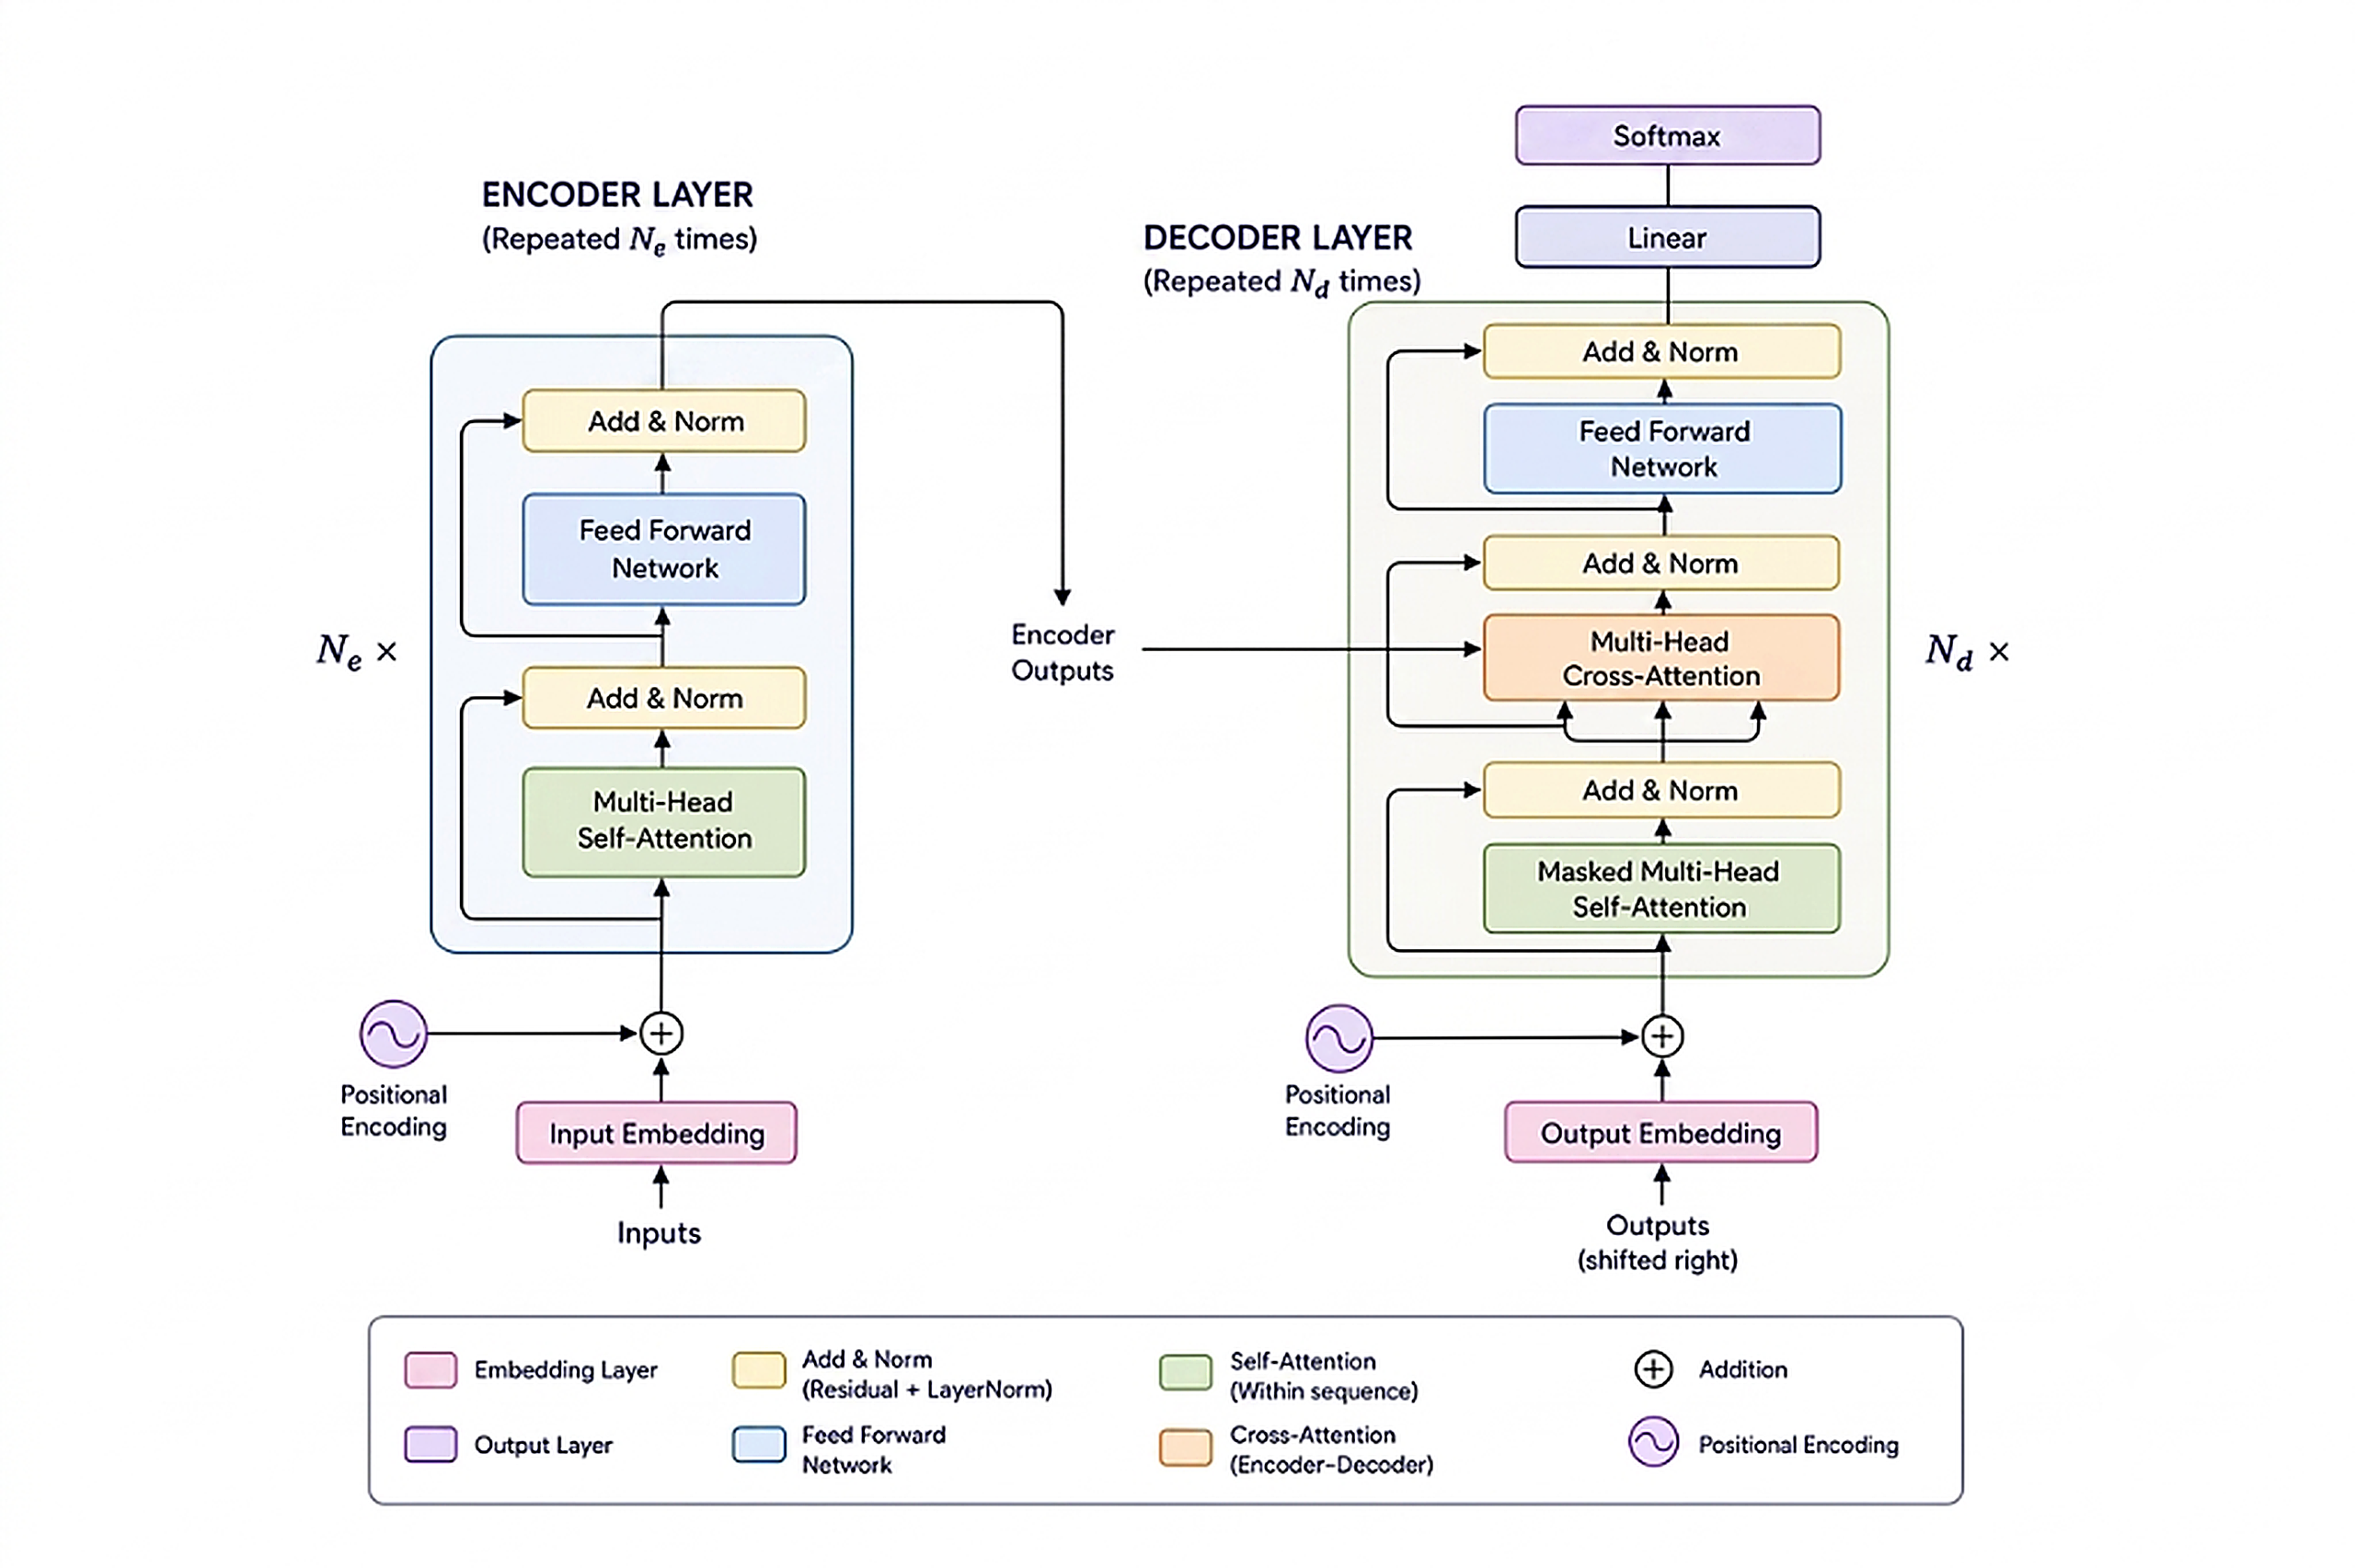
\includegraphics[width=0.88\textwidth]{figures/fig_5_transformer_architecture_pg128.png}
    \caption{The complete Transformer encoder-decoder model architecture.}
    \label{fig:transformer_architecture}
\end{figure}

\section{From Single-Head to Multi-Head Attention}
\subsection{Single-Head Self-Attention}
The Transformer begins with a single self-attention mechanism in which every token simultaneously acts as a query, key, and value. Given an input sequence $X \in \mathbb{R}^{n \times d_{model}}$, three learned linear projections generate the Query, Key, and Value matrices:
\begin{equation}
Q = X W_Q, \quad K = X W_K, \quad V = X W_V
\end{equation}
where $W_Q, W_K \in \mathbb{R}^{d_{model} \times d_k}$, and $W_V \in \mathbb{R}^{d_{model} \times d_v}$.

\begin{equation}
\text{Attention}(Q, K, V) = \text{Softmax}\left(\frac{Q K^T}{\sqrt{d_k}}\right) V
\end{equation}
where $Q K^T \in \mathbb{R}^{n \times n}$ contains the similarity between every pair of tokens.

\subsection{Why Divide by \texorpdfstring{$\sqrt{d_k}$}{sqrt(dk)}?}
The original Transformer divides the attention score by $\sqrt{d_k}$. Before applying Softmax, without this scaling factor, the variance of the dot products grows proportionally to $d_k$, causing Softmax to become highly saturated. Saturated probabilities produce extremely small gradients, slowing optimization and making training unstable. Dividing by $\sqrt{d_k}$ normalizes the variance of the attention scores, preserving stable gradients throughout training.

\begin{examplebox}[Numerical Comparison of Softmax Scaling]
Without scaling:
\begin{equation}
\text{Softmax}([16, 8, 0]) = [0.9997, 0.0003, 0.0000]
\end{equation}
The distribution is almost one-hot. The gradient of the Softmax $= 0.9997(1 - 0.9997) \approx 0.0003$. This is extremely small, hence learning is slow and gradients nearly vanish.

With scaling (e.g., dividing by $\sqrt{d_k} = \sqrt{64} = 8$):
\begin{equation}
\text{Softmax}([2, 1, 0]) = [0.665, 0.245, 0.090]
\end{equation}
Now the probabilities are much smoother: $0.665(1 - 0.665) = 0.223$. Training is therefore much more stable because useful gradients continue flowing through the network.
\end{examplebox}

\subsection{Multi-Head Attention}
A single attention head can learn only one similarity function at a time. To allow the model to capture multiple semantic relationships simultaneously, the Transformer employs Multi-Head Attention. Instead of learning one projection set, the model learns $h$ independent projection sets:
\begin{equation}
W_Q^i, W_K^i, W_V^i \quad \text{for } i = 1, \dots, h
\end{equation}

Each head computes $\text{head}_i = \text{Attention}(Q_i, K_i, V_i)$. \\
The outputs are concatenated: $H = \text{Concat}(\text{head}_1, \text{head}_2, \dots, \text{head}_h)$ and projected back into the model space:
\begin{equation}
\text{MultiHead}(Q, K, V) = \text{Concat}(\text{head}_1, \text{head}_2, \dots, \text{head}_h) W_O
\end{equation}
where $W_O \in \mathbb{R}^{h d_v \times d_{model}}$.

Example: $d_{model} = 512$ and $h = 8$, so $d_k = d_v = \frac{512}{8} = 64$.

\begin{figure}[htbp]
    \centering
    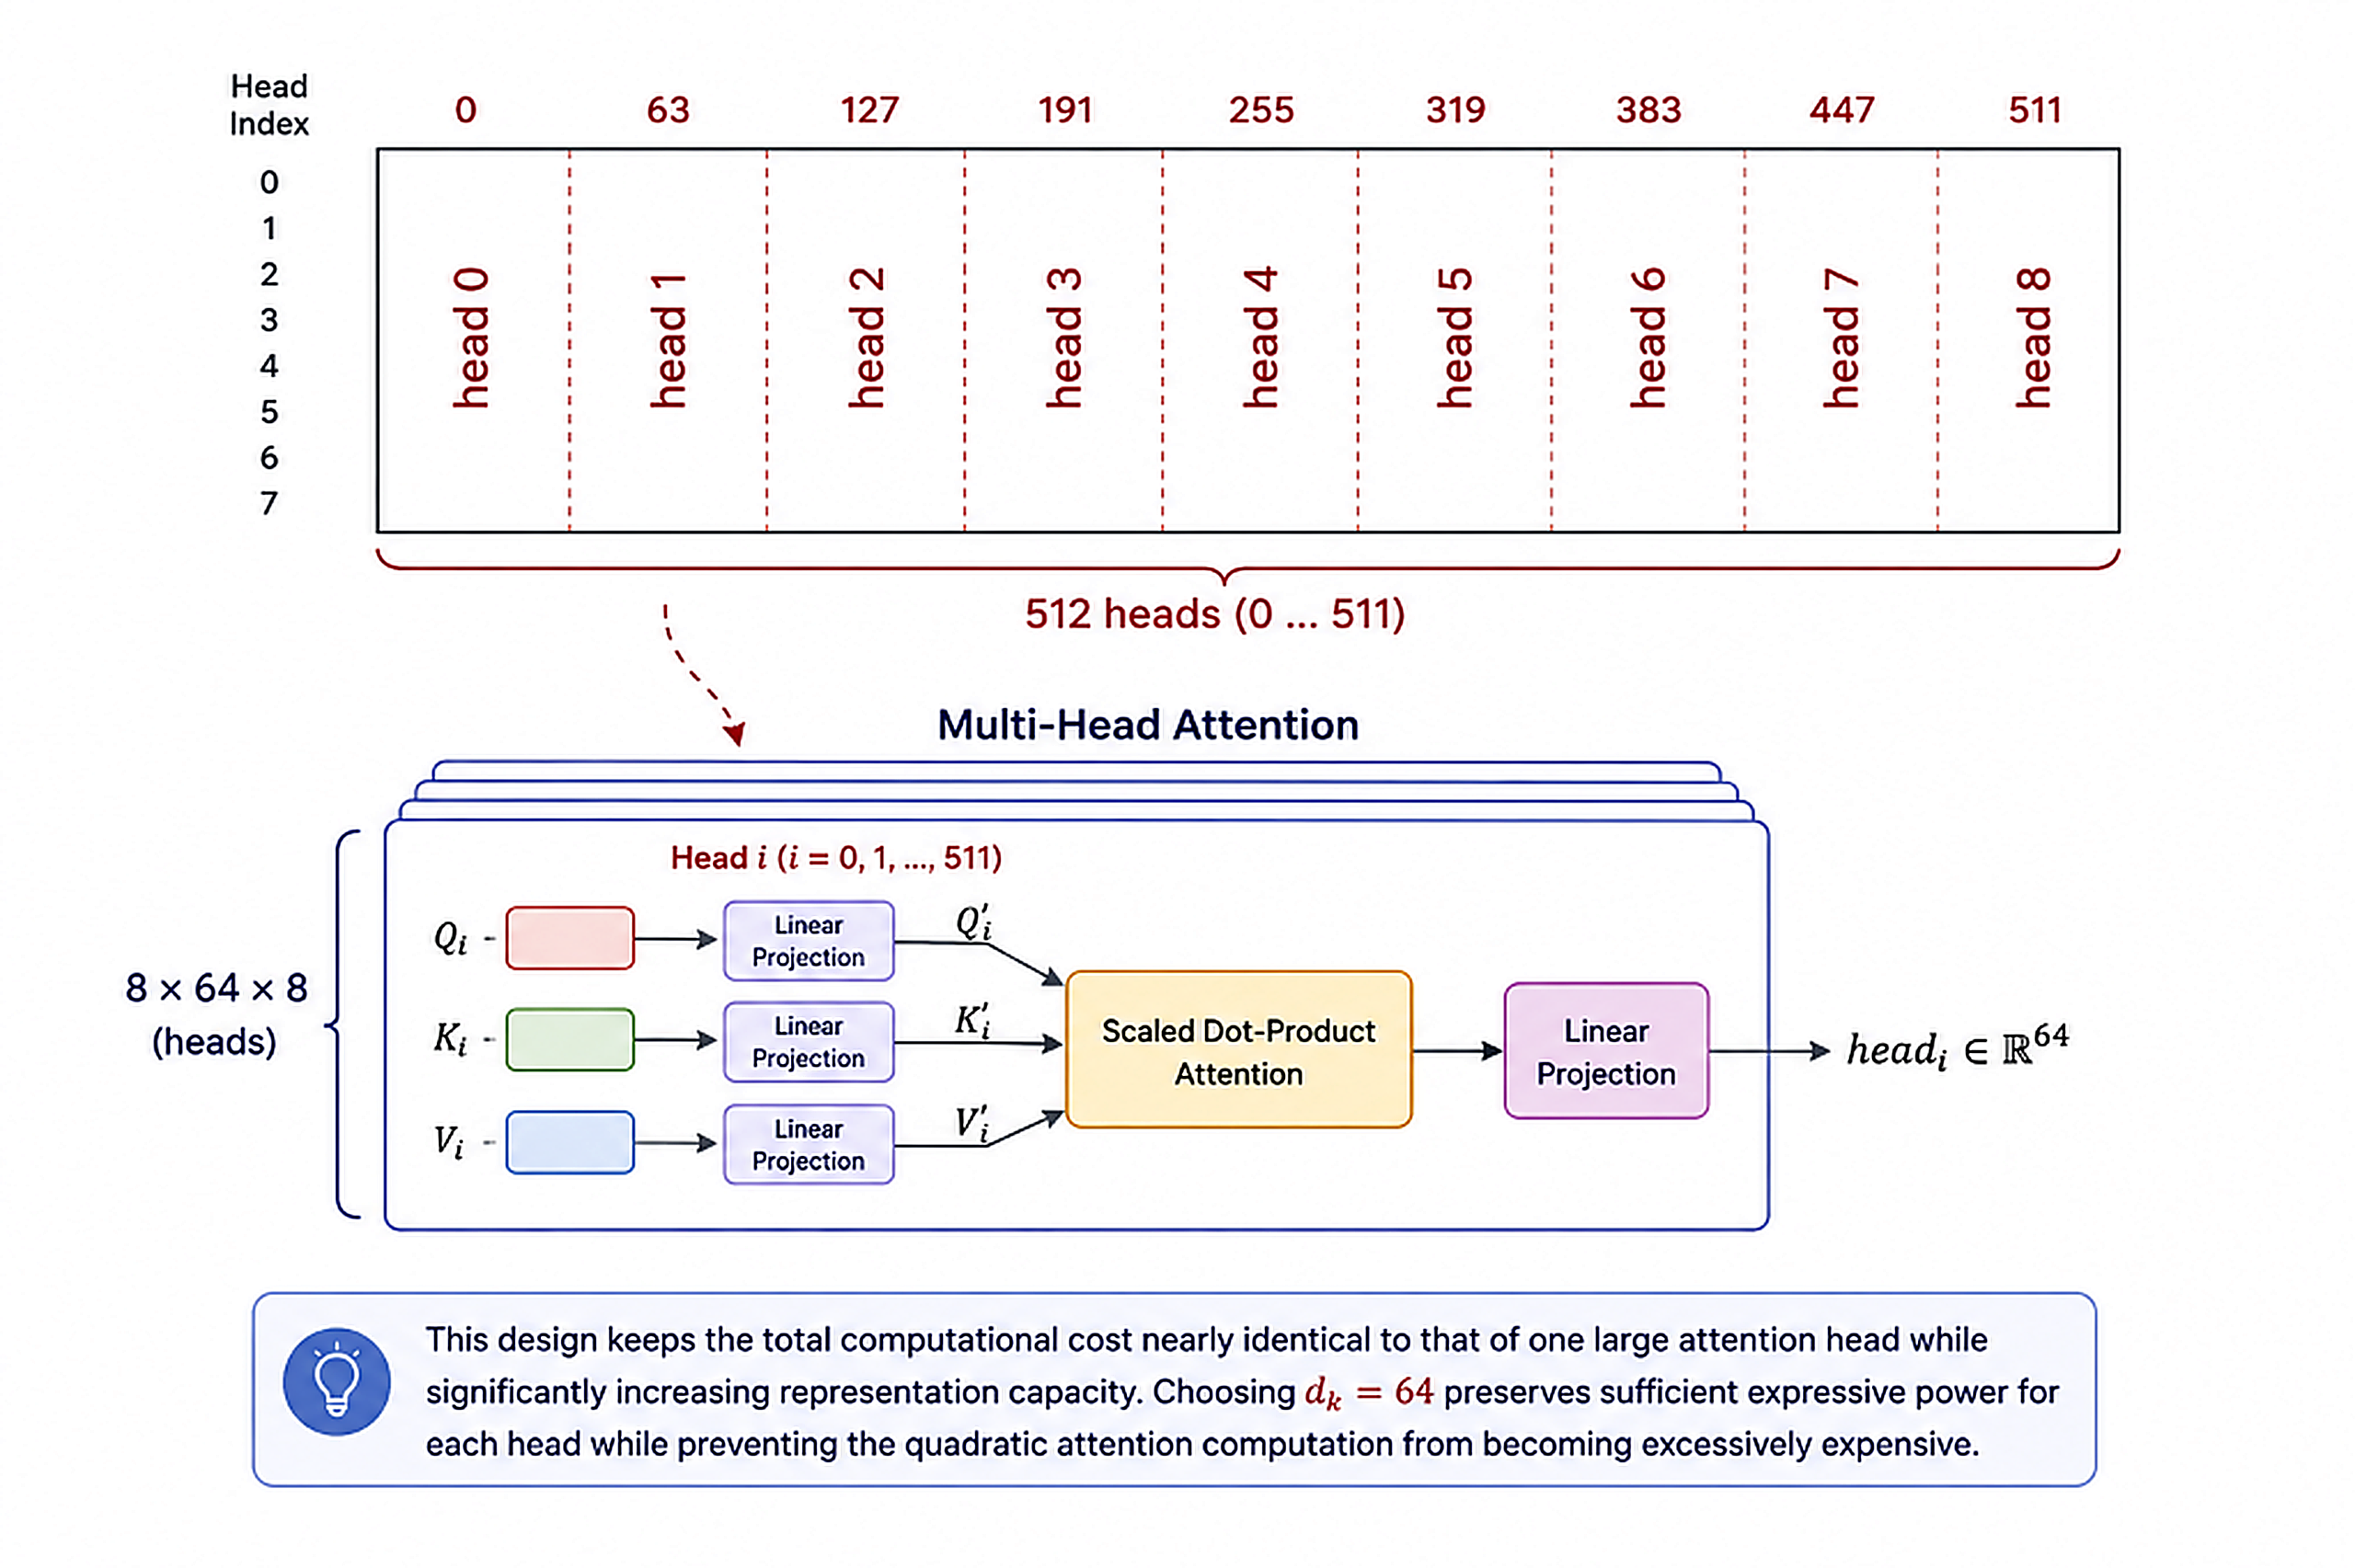
\includegraphics[width=0.92\textwidth]{figures/fig_5_multi_head_attention_pg132.png}
    \caption{Structural breakdown and linear projection flow in Multi-Head Attention.}
    \label{fig:multi_head_attention}
\end{figure}

\section{Positional Encoding}
Self-attention is permutation invariant because attention depends only on pairwise similarities and contains no information about token order. Consequently, positional information must be explicitly injected into the input representation.

The Transformer adds positional encodings directly to the token embeddings:
\begin{equation}
X' = X + PE
\end{equation}
where $X \in \mathbb{R}^{n \times d_{model}}$ and $PE \in \mathbb{R}^{n \times d_{model}}$.

Instead of learning position vectors, Transformer uses deterministic sinusoidal functions. For every position $pos$ and embedding dimension $i$:
\begin{align}
PE_{(pos, 2i)} &= \sin\left(\frac{pos}{10000^{2i/d_{model}}}\right) \\
PE_{(pos, 2i+1)} &= \cos\left(\frac{pos}{10000^{2i/d_{model}}}\right)
\end{align}
\begin{itemize}
    \item The even dimension: Use sinus function
    \item The odd dimension: Use cosinus function
\end{itemize}

Using sinusoidal functions provides unique positional representations while enabling the model to generalize to sequence lengths not observed during training, because nearby positions generate nearby vectors, and relative distances can also be inferred through linear operations.

\subsection{Why Different Frequencies?}
$10000^{2i/d_{model}}$ changes with the embedding dimension:
\begin{itemize}
    \item Low-dimension components have short wavelengths and vary rapidly with position.
    \item High-dimension components have long wavelengths and vary slowly.
\end{itemize}

\begin{figure}[htbp]
    \centering
    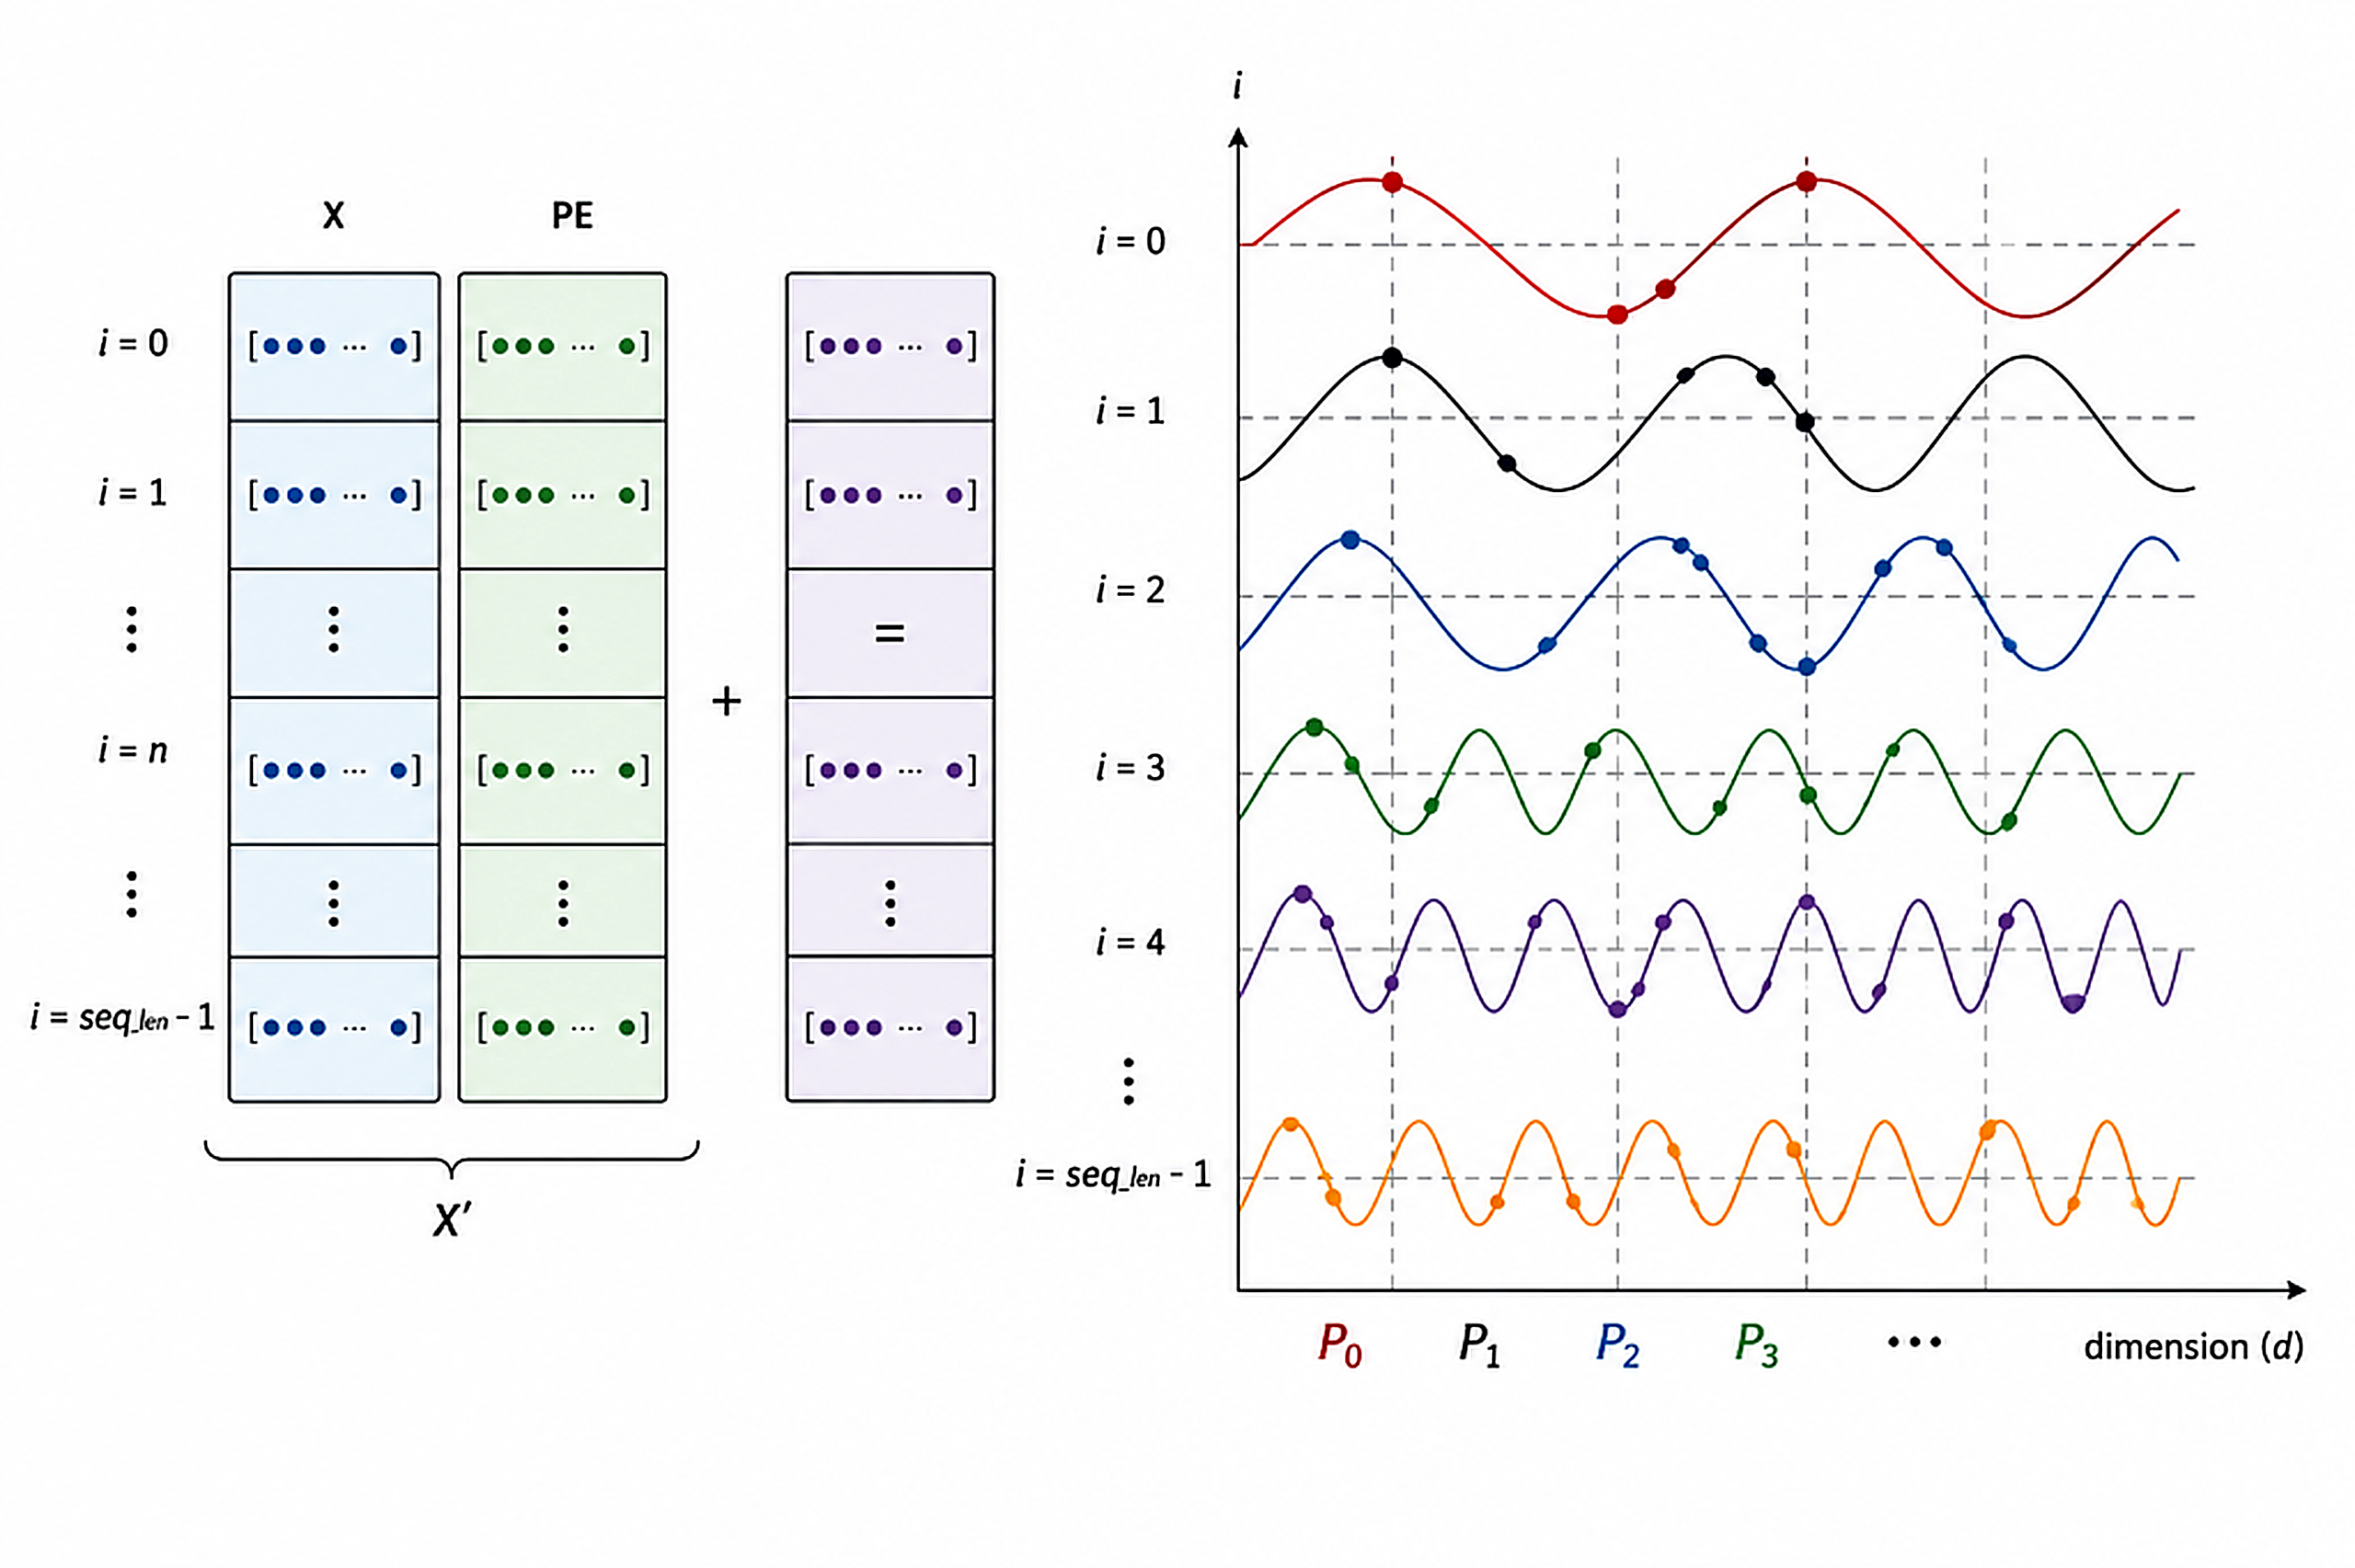
\includegraphics[width=0.88\textwidth]{figures/fig_5_positional_encoding_curves_pg134.png}
    \caption{Superposition of sinusoidal curves across embedding dimensions.}
    \label{fig:positional_curves}
\end{figure}

\begin{figure}[htbp]
    \centering
    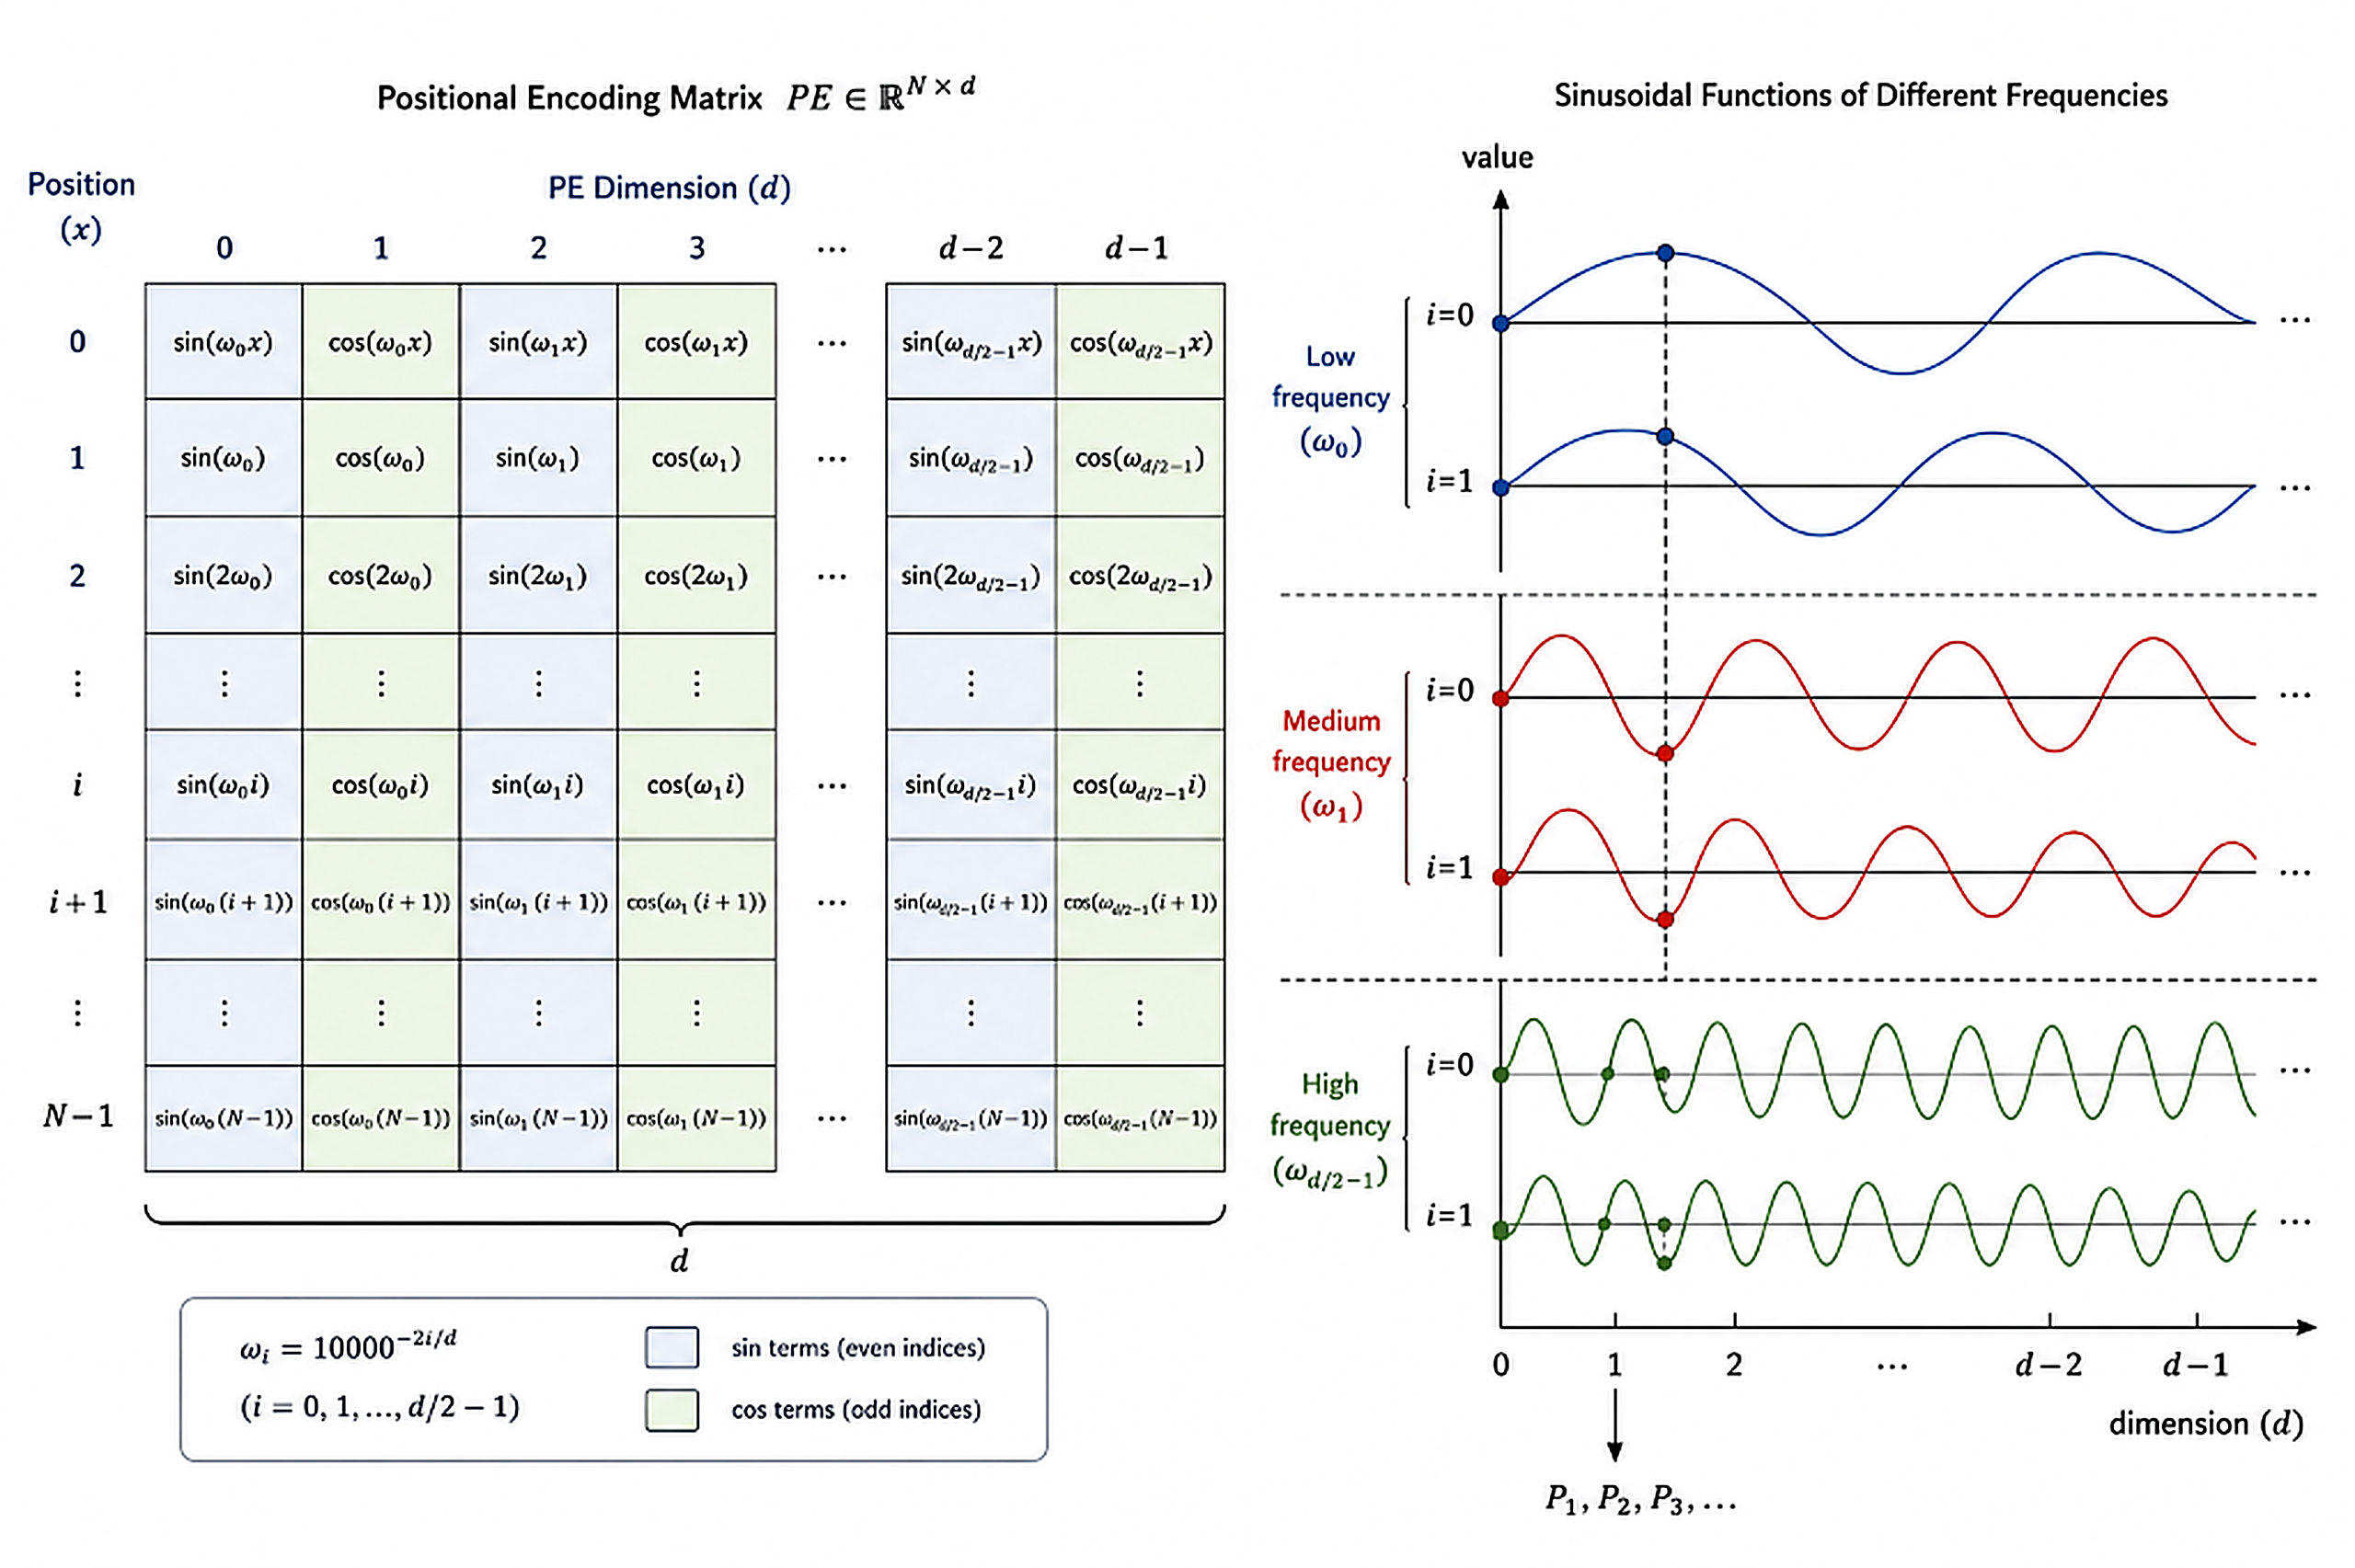
\includegraphics[width=0.88\textwidth]{figures/fig_5_positional_encoding_matrix_pg134.png}
    \caption{Structure of the Positional Encoding Matrix $PE \in \mathbb{R}^{N \times d}$.}
    \label{fig:positional_matrix}
\end{figure}

Example: $d_{model} = 8, pos = 3$. \\
The positional encoding vector becomes:
\begin{equation}
PE(3) = \left[ \sin(3), \cos(3), \sin(3/10), \cos(3/10), \sin(3/100), \cos(3/100), \sin(3/1000), \cos(3/1000) \right]
\end{equation}
Each pair of dimensions oscillates at a different frequency. Thus every position obtains a distinct vector.

\subsection{Why Sine and Cosine?}
\begin{enumerate}
    \item \textbf{Unique Representation}: Each position produces a different combination of sine and cosine values ($PE(pos_1) \neq PE(pos_2)$). For different positions, the model can distinguish every token location.
    \item \textbf{Smoothness}: Unlike one-hot position vectors, neighboring positions generate similar vectors. For example, $PE(20)$ is much closer to $PE(21)$ than $PE(200)$. This smooth transition makes optimization easier.
    \item \textbf{Relative Position Information} (The most important property): \\
    Using trigonometric identities:
    \begin{align}
    \sin(a+b) &= \sin(a)\cos(b) + \cos(a)\sin(b) \\
    \cos(a+b) &= \cos(a)\cos(b) - \sin(a)\sin(b)
    \end{align}
    Therefore, $PE(pos+k)$ can be expressed as a linear transformation of $PE(pos)$. This means the model can learn relationships such as next word and previous token.
    \item \textbf{Extrapolation to Longer Sequences}: Because the positional encoding is generated by a mathematical formula rather than learned parameters, it can be computed for positions beyond the training sequence length; however, successful extrapolation is not guaranteed.
\end{enumerate}

\subsection{Why Use Addition Instead of Concatenation?}
$X' = X + PE$. If concatenation were used instead, the dimensionality would increase (e.g. from 512 to 1024), doubling the size of the projection matrices and significantly increasing the number of parameters and computational cost.

Positional encoding enables the Transformer to model sequence order despite processing all tokens in parallel. By adding deterministic sinusoidal vectors to the input embeddings, the model receives explicit information about token positions while preserving the embedding dimensionality. The use of multiple sine and cosine frequencies produces unique, smooth, and mathematically structured representations that allow the model to infer both absolute position and relative distance. These encodings can be computed for positions beyond the training sequence length, although successful extrapolation is not guaranteed.

Although this method is elegant and parameter-free, it is rarely used in modern LLMs. Today, the most widely adopted technique is Rotary Position Embedding (RoPE), introduced in 2021. RoPE incorporates positional information by rotating the Query and Key vectors before computing attention, allowing the model to naturally capture relative positional relationships and perform better on long-context sequences.

\section{Rotary Position Embedding (RoPE)}
\begin{center}
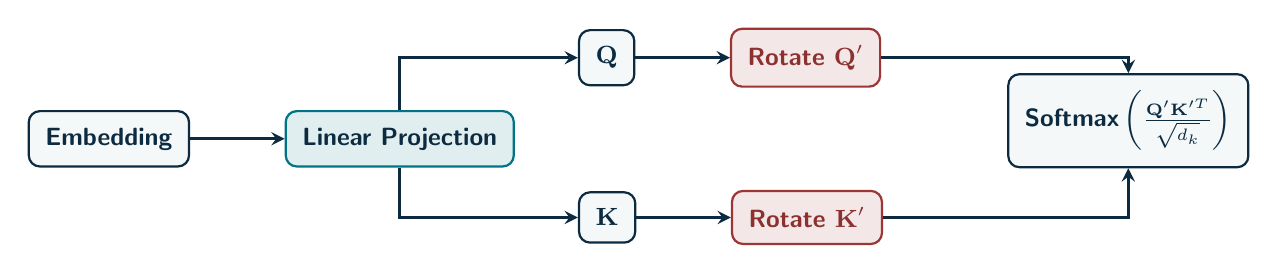
\begin{tikzpicture}[
    node distance=1.2cm, 
    auto, 
    >=stealth, 
    font=\sffamily\bfseries\small,
    mainnode/.style={draw=primaryblue, fill=boxbg, text=primaryblue, rounded corners=4pt, inner sep=6pt, line width=0.8pt},
    secnode/.style={draw=secondaryblue, fill=secondaryblue!12, text=primaryblue, rounded corners=4pt, inner sep=6pt, line width=0.8pt},
    rotnode/.style={draw=accentred, fill=accentred!12, text=accentred!90!black, rounded corners=4pt, inner sep=6pt, line width=0.8pt},
    outnode/.style={draw=primaryblue, fill=boxbg, text=primaryblue, rounded corners=4pt, inner sep=6pt, line width=0.8pt}
]
    \node [mainnode] (emb) {Embedding};
    \node [secnode, right=of emb] (proj) {Linear Projection};
    \node [mainnode, above right=0.3cm and 0.8cm of proj] (Q) {$\mathbf{Q}$};
    \node [mainnode, below right=0.3cm and 0.8cm of proj] (K) {$\mathbf{K}$};
    \node [rotnode, right=of Q] (rotQ) {Rotate $\mathbf{Q}'$};
    \node [rotnode, right=of K] (rotK) {Rotate $\mathbf{K}'$};
    \node [outnode, right=1.6cm of rotQ, yshift=-0.8cm] (attn) {$\text{Softmax}\left(\frac{\mathbf{Q}' \mathbf{K}'^T}{\sqrt{d_k}}\right)$};
    
    \draw [->, line width=1.1pt, primaryblue] (emb) -- (proj);
    \draw [->, line width=1.1pt, primaryblue] (proj) |- (Q);
    \draw [->, line width=1.1pt, primaryblue] (proj) |- (K);
    \draw [->, line width=1.1pt, primaryblue] (Q) -- (rotQ);
    \draw [->, line width=1.1pt, primaryblue] (K) -- (rotK);
    \draw [->, line width=1.1pt, primaryblue] (rotQ) -| (attn);
    \draw [->, line width=1.1pt, primaryblue] (rotK) -| (attn);
\end{tikzpicture}
\end{center}

Example: position $p = 3$, angle $\theta = 30^\circ$, Query vector $Q = \begin{bmatrix} 2 \\ 1 \end{bmatrix}$. \\
The rotation matrix is:
\begin{equation}
R = \begin{bmatrix} \cos 30^\circ & -\sin 30^\circ \\ \sin 30^\circ & \cos 30^\circ \end{bmatrix} = \begin{bmatrix} 0.866 & -0.5 \\ 0.5 & 0.866 \end{bmatrix}
\end{equation}

Multiply:
\begin{equation}
Q' = R Q = \begin{bmatrix} 0.866 & -0.5 \\ 0.5 & 0.866 \end{bmatrix} \begin{bmatrix} 2 \\ 1 \end{bmatrix} = \begin{bmatrix} 1.232 \\ 1.866 \end{bmatrix}
\end{equation}
The rotation preserves the vector's norm while incorporating position-dependent information.

\begin{advbox}[Advantages of RoPE]
\begin{itemize}
    \item Captures relative positions naturally
    \item Better performance on long-context tasks
    \item No additional trainable parameters
    \item Computationally efficient
    \item Used in most modern LLMs (e.g., LLaMA, Qwen, Gemma, DeepSeek)
\end{itemize}
\end{advbox}

\section{Position-wise Feed Forward Network}
Forward Network Transforms each token independently:
\begin{equation}
\text{FFN}(x) = W_2 \sigma(W_1 x + b_1) + b_2
\end{equation}
Dimension flow: $512 \to 2048 \to 512$. \\
$W_1 \in \mathbb{R}^{512 \times 2048}, \quad W_2 \in \mathbb{R}^{2048 \times 512}$.

\section{Residual Connections And Add \& Norm}
Deep neural networks become increasingly difficult to optimize because gradients vanish as depth increases. To alleviate this problem, every sub-layer employs a residual connection:
\begin{equation}
y = x + F(x)
\end{equation}
allowing gradients to flow directly through identity mappings.

Immediately after the residual addition, Layer Normalization is applied:
\begin{equation}
\text{LayerNorm}(x + F(x))
\end{equation}
forming the well-known Add \& Norm Operation.

Residual Connections improve optimization, while normalization stabilizes the distribution of intermediate activations, accelerates convergence, and reduces sensitivity to parameter initialization.

\subsection{Layer Normalization}
Unlike Batch Normalization, which computes statistics across the batch dimension, Layer Normalization normalizes each token independently across its feature dimensions:
\begin{equation}
\text{LayerNorm}(x) = \gamma \frac{x - \mu}{\sqrt{\sigma^2 + \epsilon}} + \beta
\end{equation}
This independence from batch statistics makes Layer Normalization particularly suitable for variable-length sequences and autoregressive inference.

\section{Transformer Encoder}
The primary objective of the encoder is not generate output tokens. Instead, its role is to transform the input sequence into a set of context-aware representation that capture the semantic and syntactic relationships among all tokens. These contextual representations serve as the knowledge base from which the decoder later generates the target sequence.

Unlike an RNN encoder, which compresses information sequentially into hidden states, the Transformer encoder processes the entire sequence simultaneously through stacked attention layers, allowing every token to directly exchange information with every other token.

The output vector now contains contextual information from the entire sentence rather than representing only the corresponding token.

The output has exactly the same dimensions as the input:
\begin{equation}
X \in \mathbb{R}^{n \times 512} \longrightarrow U \in \mathbb{R}^{n \times 512}
\end{equation}
$n$: sequence length (tokens).

\subsection{Encoder Workflow and Architecture}
\textbf{1. Input to encoder:}
\begin{enumerate}
    \item Tokenization
    \item Embedding
    \item Positional Encoding
\end{enumerate}

Therefore the encoder receives:
\begin{equation}
X = \begin{bmatrix} x_1 \\ x_2 \\ \vdots \\ x_n \end{bmatrix} \in \mathbb{R}^{n \times 512}
\end{equation}

\textbf{2. Encoder Architecture:} \\
The original Transformer stacks $N = 6$ identical encoder blocks. Each block has exactly the same architecture but different learned parameters:
\begin{align}
U^{(0)} &= X \\
U^{(\ell)} &= \text{Encoder Block}^{(\ell)}\left(U^{(\ell-1)}\right), \quad \ell = 1, \dots, 6 \\
\text{The final encoder output is } U &= U^{(6)}
\end{align}

\subsection{Encoder Block Operations}
Each encoder block performs four operations sequentially: \\
$\text{Multi-Head Self-Attention} \longrightarrow \text{Add \& Norm} \longrightarrow \text{Feed Forward Network} \longrightarrow \text{Add \& Norm}$.

Although the dimensionality never changes, the representation becomes increasingly richer after every block.

\textbf{Step 1: Multi-Head Self-Attention} \\
The block first compute:
\begin{equation}
Q = X W_Q, \quad K = X W_K, \quad V = X W_V
\end{equation}
Attention produces:
\begin{equation}
H = \text{MultiHead}(Q, K, V)
\end{equation}
Dimension: $X \in \mathbb{R}^{n \times 512} \implies H \in \mathbb{R}^{n \times 512}$. \\
Every token now contains information collected from all other tokens.

\textbf{Step 2: Add \& Norm} \\
The attention output is added back to its input:
\begin{equation}
R_1 = X + H
\end{equation}
Layer Normalization is then applied:
\begin{equation}
Z = \text{LayerNorm}(R_1) \in \mathbb{R}^{n \times 512}
\end{equation}
The residual path preserves information from previous layers while normalization stabilizes optimization.

\textbf{Step 3: Feed Forward Network} \\
Each token independently passes through the same feed-forward network:
\begin{align}
F &= \text{FFN}(Z) \\
\text{FFN}(x) &= W_2 \text{ReLU}(W_1 x + b_1) + b_2
\end{align}
First layer: $512 \to 2048$, Second layer: $2048 \to 512$. \\
$Z \in \mathbb{R}^{n \times 512}$.

\textbf{Step 4: Add \& Norm} \\
A residual connection is applied:
\begin{equation}
R_2 = Z + F, \quad U = \text{LayerNorm}(R_2) \in \mathbb{R}^{n \times 512}
\end{equation}
This completes one encoder block.

\textbf{3. Stacking Encoder Blocks:} \\
The output of one encoder block immediately becomes the input of the next:
\begin{equation}
U^{(1)} \to U^{(2)} \to \dots \to U^{(6)}
\end{equation}
No block change tensor size $\in \mathbb{R}^{n \times 512}$.

Each successive block refines the contextual representation by repeatedly combining global information through attention and non-linear feature transformations through the feed-forward network.

\subsection{Encoder Output}
After the sixth encoder block, the encoder produces:
\begin{equation}
U = \begin{bmatrix} u_1 \\ u_2 \\ \vdots \\ u_n \end{bmatrix} \in \mathbb{R}^{n \times 512}
\end{equation}
Each vector $u_i$ now is a contextual representation that encodes information about the entire input sequence. Every token representation has been updated through multiple rounds of self-attention, allowing it to capture long-range dependencies and global context.

\section{Transformer Decoder}
The decoder is responsible for generating the target sequence one token at a time. The encoder built contextual representations of the input. The decoder uses these representation to predict the next output token autoregressively. At each decoding step, it conditions its prediction on two sources of information.

Consequently, the decoder learns the conditional probability distribution:
\begin{equation}
P(y_1, \dots, y_T \mid x_1, \dots, x_n) = \prod_{t=1}^T P(y_t \mid y_{<t}, X)
\end{equation}
$X$: the source sequence \\
$y_{<t}$: all previously generated target tokens.

Unlike the encoder, the decoder cannot process all target tokens independently during inference because each prediction depends on the previous ones.

\subsection{Decoder Architecture}
The original Transformer stacks $N = 6$ identical decoder block. Each block consists of: \\
$\text{Masked Multi-Head Self-Attention} \longrightarrow \text{Add \& Norm} \longrightarrow \text{Encoder-Decoder Attention} \longrightarrow \text{Add \& Norm} \longrightarrow \text{Feed Forward Network} \longrightarrow \text{Add \& Norm}$.

\subsection{Decoder Block Breakdown}
\textbf{Step 1: Masked Multi-Head Self-Attention} \\
Attention is computed as:
\begin{equation}
\text{Attention} = \text{Softmax}\left(\frac{Q K^T + M}{\sqrt{d_k}}\right) V
\end{equation}

Mask $M$:
\begin{equation}
\begin{bmatrix}
0.31 & 0.36 & 0.55 & 0.02 & 0.3 \\
0.25 & 0.13 & 0.21 & 0.01 & 0.17 \\
0.26 & 0.23 & 0.35 & 0.01 & 0.22 \\
0.01 & 0.04 & 0.07 & 0.0 & 0.02 \\
0.14 & 0.13 & 0.20 & 0.01 & 0.12
\end{bmatrix}
+
\begin{bmatrix}
0 & -\infty & -\infty & -\infty & -\infty \\
0 & 0 & -\infty & -\infty & -\infty \\
0 & 0 & 0 & -\infty & -\infty \\
0 & 0 & 0 & 0 & -\infty \\
0 & 0 & 0 & 0 & 0
\end{bmatrix}
=
\begin{bmatrix}
0.31 & -\infty & -\infty & -\infty & -\infty \\
0.25 & 0.13 & -\infty & -\infty & -\infty \\
0.26 & 0.23 & 0.35 & -\infty & -\infty \\
0.01 & 0.04 & 0.07 & 0.0 & -\infty \\
0.14 & 0.13 & 0.20 & 0.01 & 0.12
\end{bmatrix}
\end{equation}
Thus, the token at position $i$ can only attend to itself and all previous, but never to future tokens.

This masking mechanism prevents information leakage during training, ensuring that the decoder learns to predict the next token using only the previously generated content.

* The reason for using $-\infty$: we want the masked positions to receive exactly zero attention probability after applying Softmax, e.g., $\text{Softmax}([2, 1, -\infty]) = [0.665, 0.335, 0]$.

\textbf{Step 2: Add \& Norm} \\
Residual connection: $R_1 = Y + H, \quad Z = \text{LayerNorm}(R_1) \in \mathbb{R}^{t \times 512}$.

\textbf{Step 3: Encoder-Decoder Attention (Cross-Attention)} \\
This is the only operation that connects the decoder to the encoder. Unlike self-attention, the queries originate from the decoder, and the keys and values originate from the encoder output:
\begin{align}
Q &= Z W_Q \\
K &= U W_K \\
V &= U W_V
\end{align}
The attention becomes: $\text{Attention}(Q, K, V) = \text{Softmax}\left(\frac{Q K^T}{\sqrt{d_k}}\right) V$. \\
Output $C \in \mathbb{R}^{t \times 512}$ where $Q \in \mathbb{R}^{t \times 64}, K \in \mathbb{R}^{n \times 64}, V \in \mathbb{R}^{n \times 64}$ ($512/8 = 64$).

Unlike self-attention, where each token attends to the target sequence itself, cross-attention enables every decoder position to retrieve the most relevant information from the encoded source sequence.

\textbf{Step 4: Add \& Norm} \\
The output of the cross-attention is combined with the residual connection:
$R_2 = Z + C, \quad D_1 = \text{LayerNorm}(R_2) \in \mathbb{R}^{t \times 512}$.

\textbf{Step 5: Feed Forward Network} \\
Each decoder representation is independently transformed through the position-wise feed-forward network:
\begin{equation}
\text{FFN}(x) = W_2 \text{ReLU}(W_1 x + b_1) + b_2
\end{equation}
$512 \to 2048 \to 512$. Applied to the entire sequence: $t \times 512 \to t \times 2048 \to t \times 512$.

\textbf{Step 6: Add \& Norm} \\
The final residual connection is computed: $R_3 = \text{FFN} + R_2$, $D = \text{LayerNorm}(R_3)$. \\
This is complete one decoder block.

\subsection{Stacking Decoder Blocks and Prediction}
\textbf{Stacking Decoder Blocks:} \\
The Transformer stacks 6 decoder blocks:
\begin{align}
D^{(0)} &= Y \\
D^{(\ell)} &= \text{Decoder Block}^{(\ell)}\left(D^{(\ell-1)}, U\right), \quad \ell = 1, \dots, 6
\end{align}
The encoder output is shared by every decoder block, while the decoder representation is progressively refined.

\textbf{Final Decoder Output:} \\
After the sixth decoder block, $D \in \mathbb{R}^{t \times 512}$. \\
This matrix contains contextual representations of every generated target token, enriched by both the previously generated target sequence and the encoded source sequence. However, these vectors are not yet predicted words.

To produce the final prediction, each decoder output vector is passed through a linear projection:
\begin{equation}
Z = D W_{voc} + b, \quad W_{voc} \in \mathbb{R}^{512 \times |V|}
\end{equation}
$|V|$ is the vocabulary size: vocabulary is the set of all tokens that the model knows and can predict.

The resulting logits $Z \in \mathbb{R}^{t \times |V|}$ are converted into probabilities using $P = \text{Softmax}(Z)$. The token with the highest probability becomes the next generated token.

\section{Key-Value Cache (KV Cache)}

The Primary Goal of a Transformer during inference is to generate One Token at a time. This Process is Known as autoregressive Generation, Meaning that each newly generated Token depends on all Previously generated tokens.

Unlike training, where the entire target Sequence is available simultaneously, inference has access only to The Tokens that have already been Generated, Therefore, The model must repeatedly execute the decoder every new token until the Sequence is complete.

Suppose we want The model to Generate the Sentence: \\


\textit{The cat is sleeping on the sofa.}

\begin{center}
\begin{tabular}{l l}
$\langle \text{BOS} \rangle$
& $\rightarrow$ Predict ``The'' \\[4pt]

$\langle \text{BOS} \rangle$ The
& $\rightarrow$ Predict ``cat'' \\[4pt]

$\langle \text{BOS} \rangle$ The cat
& $\rightarrow$ Predict ``is'' \\[4pt]

$\langle \text{BOS} \rangle$ The cat is
& $\rightarrow$ Predict ``sleeping'' \\[4pt]

$\langle \text{BOS} \rangle$ The cat is sleeping
& $\rightarrow$ Predict ``on'' \\[4pt]

$\langle \text{BOS} \rangle$ The cat is sleeping on
& $\rightarrow$ Predict ``the'' \\[4pt]

$\langle \text{BOS} \rangle$ The cat is sleeping on the
& $\rightarrow$ Predict ``sofa'' \\[4pt]

$\langle \text{BOS} \rangle$ The cat is sleeping on the sofa
& $\rightarrow$ $\langle \text{EOS} \rangle$
\end{tabular}
\end{center}

Notice that The input sequence grows after every generation step, At step $t$, The decoder receives all Tokens Generated up to step $t-1$.

\subsection{The Central Idea behind KV Cache}

The Central Idea behind KV cache is simple but Powerful: Previous token never change after They are generated, Consequently, their Key and Value vectors remain Constant and do not need to be recomputed.

By storing these vectors in memory and reusing them at every generation step, the decoder avoids redundant computation and computes the query, key, and value only for the newest token. This optimization dramatically accelerates inference while producing exactly the same output as the original Transformer without caching.

Understanding the KV cache begins with recognizing the fundamental difference between training and inference.

\paragraph{During Training}
The model already knows the complete target sentence because it is provided by the training dataset. Using teacher forcing, the entire shifted target sequence is fed into the decoder simultaneously. For example, if the target sentence is ``The cat is sleeping,'' the decoder receives $\langle \text{BOS} \rangle$ ``the cat is sleeping'' in a single forward pass. Because all tokens are processed in parallel, the Transformer computes attention for every position at once.

\paragraph{During Inference}
The future words are unknown. The decoder initially receives only $\langle \text{BOS} \rangle$ and predicts the first token. It runs again for each generated token, performing $n$ separate forward passes. The computational cost therefore increases with sequence length, and this repeated computation becomes the primary bottleneck during inference.

\subsection{The Motivation for KV Cache}

The key observation behind the KV cache is that previously generated tokens do not change during autoregressive generation. Once a token has been processed, its key and value vectors remain constant and are identical in all subsequent decoding steps.

\paragraph{Example (Without KV Cache)}
\begin{itemize}
    \item Step 1: Compute $Q, K, V$ for token 1
    \item Step 2: Compute $Q, K, V$ for token 1 and 2
    \item Step 3: Compute $Q, K, V$ for tokens 1 and 2 and 3
\end{itemize}

The KV cache eliminates this inefficiency by storing the computed key and value vectors in memory. During subsequent decoding steps, the model reuses the cached keys and values and computes new projections only for the most recently generated token. The query vector is not cached because it is always computed from the current token being processed.

\paragraph{After Using the KV Cache}
\begin{itemize}
    \item Step 1: Compute $Q$, $K$, and $V$ for token 1; store $K$ and $V$.
    \item Step 2: Compute $Q$, $K$, and $V$ for token 2; reuse the $K$ and $V$ of token 1, then store those of token 2.
    \item Step 3: Compute $Q$, $K$, and $V$ for token 3; reuse the $K$ and $V$ of tokens 1 and 2, then store those of token 3.
\end{itemize}

The decoder no longer recomputes Keys and Values for Previous tokens.

This optimization Produces exactly The Same model Output as the Original Transformer while Significantly reducing The Computational Cost of autoregressive inference, making real-time text Generation Practical for modern Large language models.

\subsection{Equation \& Complexity}

The new Equation becomes:
\begin{equation}
\text{Attention} = \text{Softmax}\left(\frac{Q_t K_{\text{cache}}^T}{\sqrt{d_k}}\right) \cdot V_{\text{cache}}
\end{equation}

\begin{align*}
K_{\text{cache}} &\in \mathbb{R}^{B \times h \times L \times d_k} \\
V_{\text{cache}} &\in \mathbb{R}^{B \times h \times L \times d_k}
\end{align*}
$B$: Batch size, $h$: N. of heads, $L$: Sequence length, $d_k$: Head dimention.

\paragraph{Complexity}
\begin{itemize}
    \item Without KV cache: $\mathcal{O}(n^2)$
    \item With KV cache: $\mathcal{O}(n)$
\end{itemize}

KV cache exchange Computation for memory, The memory needs to grows linearly with the Context length:
\begin{equation}
\text{Memory} = 2 B h L d_k
\end{equation}
(Key, Value)

As the context length increase, The cache Consumes more Gpu memory (VRAM) which becomes one of The Primary limitations of long-context language Models.

\paragraph{Advantages}
\begin{itemize}
    \item Eliminates redundant computation of Previously generated Keys and Values
    \item Significantly accelerates autoregressive (generate one token at time) inference
    \item Reduces Computational Complexity and Key, value Projection from $\mathcal{O}(n^2)$ to $\mathcal{O}(n)$
    \item Produces exactly The Same outputs as the Original Transformer without caching
    \item Used by virtually all modern decoder-only Large language models
\end{itemize}

\paragraph{Limitation}
\begin{itemize}
    \item Requires additional Gpu memory (vRAM) to Store The cache
    \item The Memory consumption increase linearly with the context length
    \item Does not improve training Speed because memory-bound due to the large cache size
\end{itemize}

\section{Modern Variants of KV Cache}

\subsection{I) Multi-Query Attention (MQA)}

\paragraph{Motivation} In standard multi-head attention, every attention head has its own query, key, and value projections. Consequently, each head requires its own key and value cache, leading to high memory consumption during inference.

MQA reduces memory overhead by allowing all attention heads to share a single key projection and a single value projection, while each head retains its own query projection.

\paragraph{Instead of}
\begin{align*}
\text{Head 1} &\longrightarrow Q_1, K_1, V_1 \\
\text{Head 2} &\longrightarrow Q_2, K_2, V_2 \\
&\;\;\dots \\
\text{Head } h &\longrightarrow Q_h, K_h, V_h
\end{align*}

\paragraph{MQA becomes}
\begin{align*}
\text{Head 1} &\longrightarrow Q_1 \\
\text{Head 2} &\longrightarrow Q_2 \\
&\;\;\dots \\
\text{Head } h &\longrightarrow Q_h \\
&\quad (\text{Shared } K \text{ and } V)
\end{align*}

\begin{figure}[H]
    \centering
    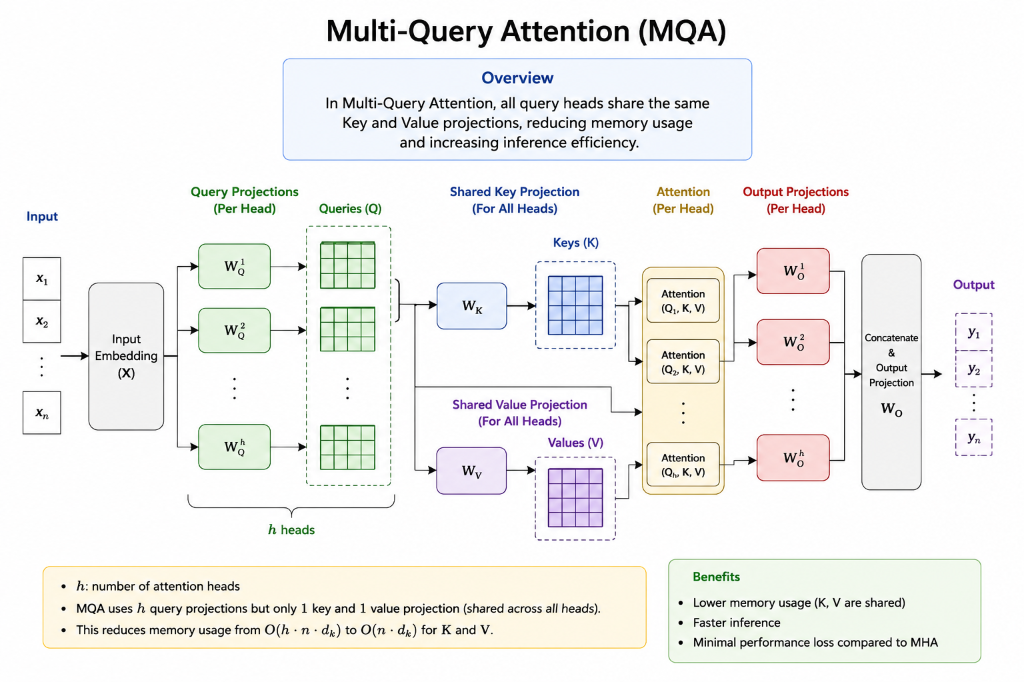
\includegraphics[width=0.95\textwidth]{figures/fig_5_1_gqa.png}
    \caption{Multi-Query Attention (MQA)}
    \label{fig:5_7_mqa}
\end{figure}

\paragraph{Advantages}
\begin{itemize}
    \item Much smaller KV cache
    \item Lower Gpu memory usage
    \item Faster inference
    \item Particularly effective for very LLMs
\end{itemize}

\paragraph{Limitation} Sharing a Single Key and Value across all heads slightly reduces The representational Capacity of The Attention mechanism.

\subsection{II) Grouped-Query Attention (GQA)}

\paragraph{Motivation} MQA greatly reduces memory usage but may sacrifice some modeling capacity because all heads share the same key and value.

GQA provides a compromise between standard multi-head attention and MQA.

\paragraph{Architecture} Instead of one key and value per head or one shared key and value for all heads, attention heads are divided into groups.

Each group shares a key and value projection.

\paragraph{For example} Eight query heads and two KV groups:
\begin{itemize}
    \item Heads 1 to 4: shared $K_1$ and shared $V_1$
    \item Heads 5 to 8: shared $K_2$ and shared $V_2$
\end{itemize}

\begin{figure}[H]
    \centering
    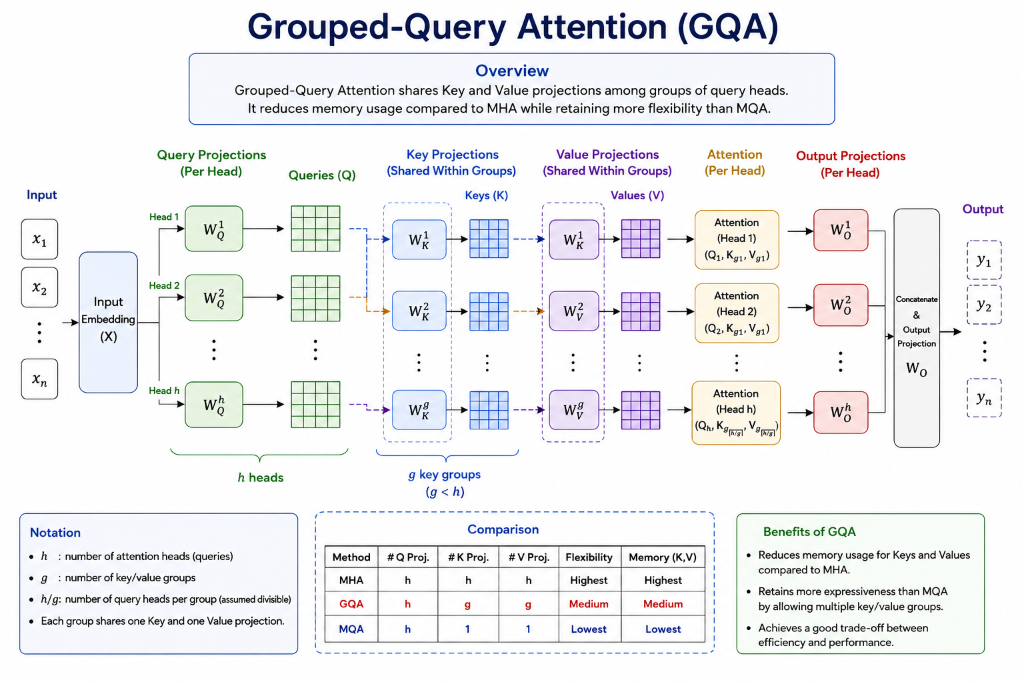
\includegraphics[width=0.95\textwidth]{figures/fig_5_1_mla.png}
    \caption{Grouped-Query Attention (GQA)}
    \label{fig:5_8_gqa}
\end{figure}

\paragraph{Advantages}
\begin{itemize}
    \item Smaller KV cache than Standard Multi-Head Attention
    \item Better modeling capacity than MQA
    \item Excellent balance between memory efficiency and model quality
    \item Widely adopted in modern LLMs
\end{itemize}

\paragraph{Limitation} Although much smaller than standard Multi-Head Attention, The cache remains larger than in MQA.

\subsection{III) Multi-Head Latent Attention (MLA) DeepSeek}

This is currently one of the biggest innovation.

Instead of Storing Keys and Values directly, DeepSeek stores a Compressed latent representation.

\begin{center}
Token $\longrightarrow$ Latent Compression $\longrightarrow$ Small Latent Vector $\longrightarrow$ Cache Latent $\longrightarrow$ when needed Reconstruct $K, V$
\end{center}

So instead of Store $K$ and $V$, DeepSeek stores $z$ (latent vector).

\begin{itemize}
    \item $K$: 512 number, $V$: 512 number, store: 1024 numbers
    \item Latent $\longrightarrow$ 128 numbers
\end{itemize}

Memory is dramatically reduced.

\begin{figure}[H]
    \centering
    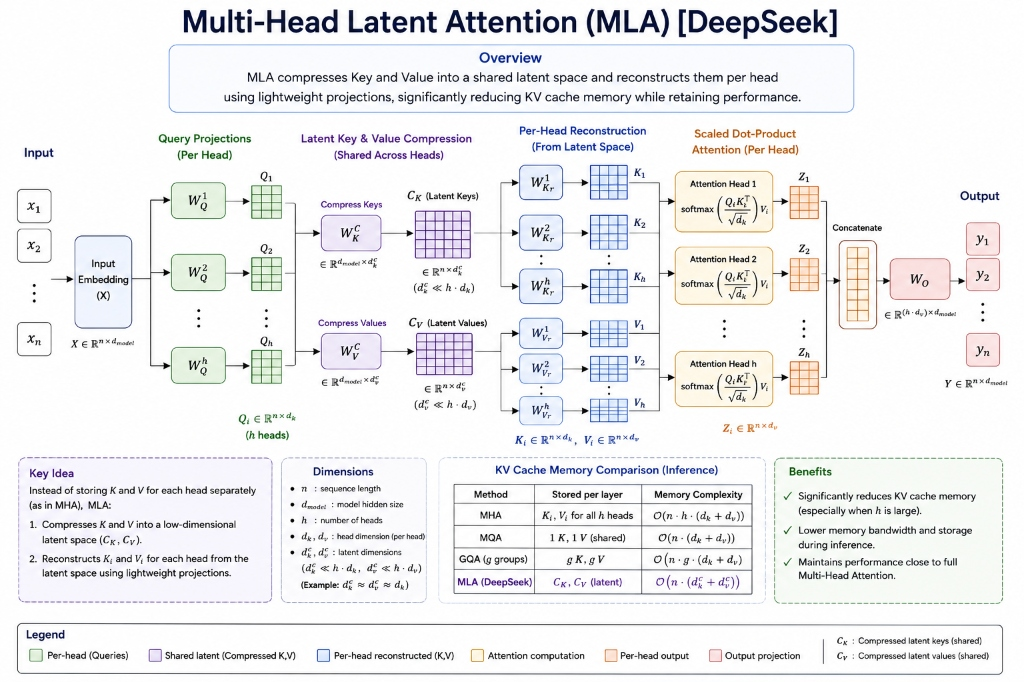
\includegraphics[width=0.98\textwidth]{figures/fig_5_1_comparison.jpg}
    \caption{Multi-Head Latent Attention (MLA) [DeepSeek]}
    \label{fig:5_9_mla}
\end{figure}

\paragraph{Advantages}
\begin{itemize}
    \item Much smaller Kv cache
    \item Longer Context
    \item Better Than GQA for memory
    \item Lower VRAM
    \item Faster inference
\end{itemize}

\begin{figure}[H]
    \centering
    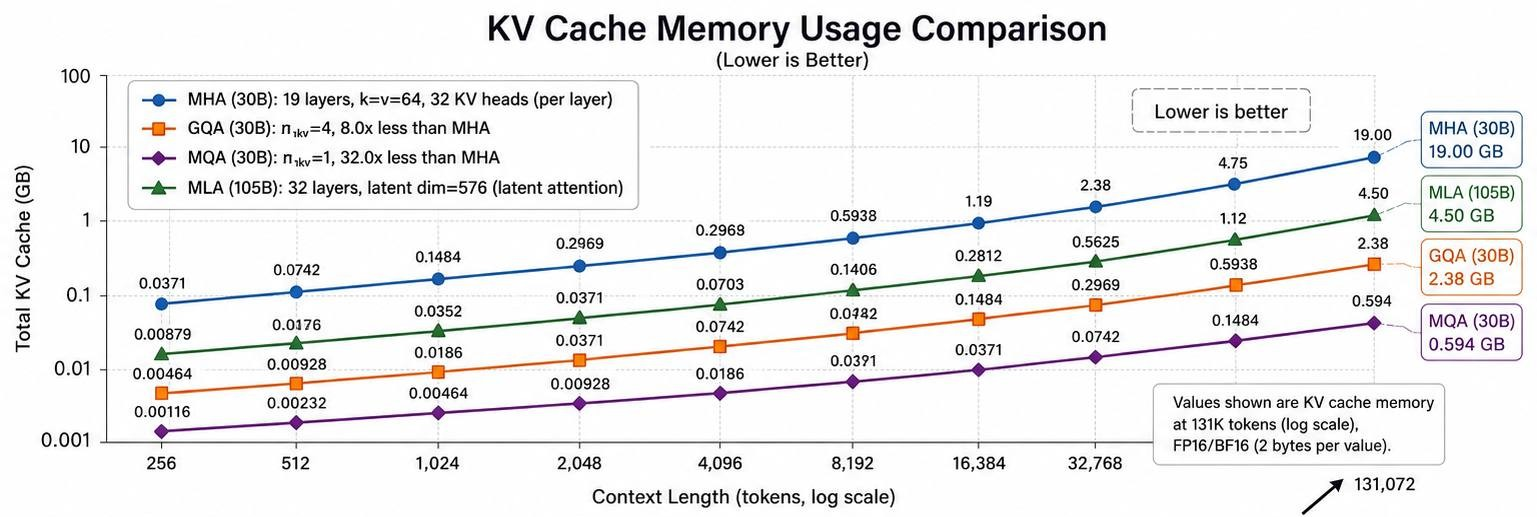
\includegraphics[width=0.95\textwidth]{figures/kv1.jpg}
    \caption{KV Cache Memory Usage Comparison}
    \label{fig:5_6_comparison}
\end{figure}

\begin{figure}[H]
    \centering
    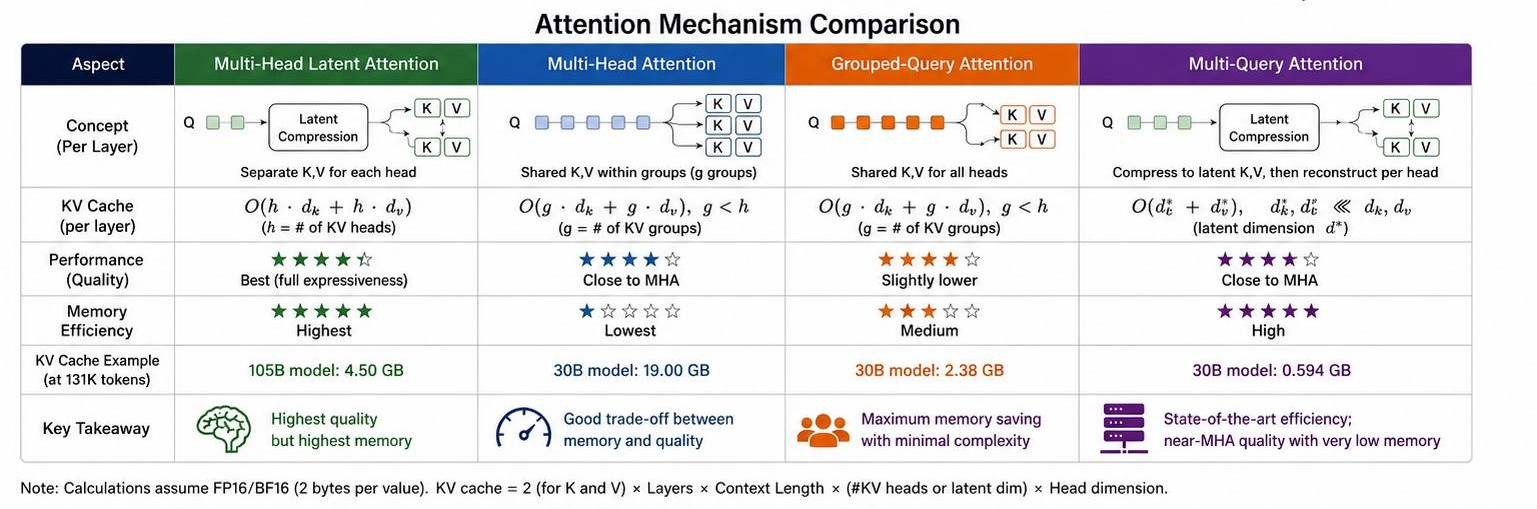
\includegraphics[width=0.95\textwidth]{figures/kv2.jpg}
\end{figure}
\section{Encoder-Only Transformers (BERT Family)}

The Original Transformer was designed for Seq2Seq tasks, where both an encoder and a decoder are required. However, many NLP applications require only language understanding and Never generate new Text as:
\begin{itemize}
    \item Text Classification
    \item Sentiment Analysis
    \item Named Entity Recognition (NER)
    \item Spam detection
    \item Semantic Similarity
    \item Document Classification
\end{itemize}

The Original Transformer (Encoder-Decoder) was Specifically designed for Seq2Seq tasks as machine translation. The researchers recognized That The encoder alone already Produces rich Contextual representations of the input Sequence. Every Encoder layer allows each token to Attend to every other token through bidirectional Self Attention, Producing Contextual embeddings that Capture both local and Global Semantic relationships.

Therefore, if The Goal is to understand text rather Than generate it, The encoder already Provides everything that is needed. This Observation led to a fundamental architecture simplification: Remove the decoder entirely and Retain only the encoder stack.

\subsection{BERT (Bidirectional Encoder Representation from Transformer)}

Based on This idea, Google introduced BERT in 2018 the first Large-scale Pretrained encoder-only Transformer.

BERT consists only of Input $\longrightarrow$ Encoder $\longrightarrow$ Task-specific Output Layer.

The decoder is Completely removed because BERT is designed for understanding rather than generation.

After Several encoder layer, every token contains information from The entire input Sequence. These Contextual embeddings Capture lexical meaning, syntax, semantics and long-range dependencies making them suitable for a wide variety of downstream NLP tasks.

Instead of Generating Text, BERT directly uses these Contextual Representations to make Predictions through a lightweight task-specific output layer.

\paragraph{BERT Architecture}
Unlike the Original Transformer encoder architecture, BERT introduces several modifications to The input representation and training procedure that enable it to learn deep bidirectional contextual representation from Large-scale unlabeled text.

The architecture primarily consists of stacked encoder blocks:
\begin{itemize}
    \item BERT-Base: 12 stacked encoder layers, 12 attention heads and 110 million parameters.
    \item BERT-Large: 24 stacked encoder layers, 16 attention heads and 340 million parameters.
\end{itemize}

BERT introduces a richer input representation by combining token, position, segment embedding:
\begin{equation}
E = E_{\text{token}} + E_{\text{pos}} + E_{\text{segment}}
\end{equation}

BERT Learns Positional Embeddings during Training and produces Contextual representations for every input token which are later used for various downstream NLP tasks.

\subsection{WordPiece Tokenization}

WordPiece Tokenization is a sub-word-based algorithm that enables BERT to efficiently represent text using a fixed-size Vocabulary. By decomposing words into smaller subword units, it Greatly reduces the out-of-vocabulary problem.

Suppose the Vocabulary contains: Play, Playing, Played, Player. Now consider the word playfulness if it not exist in the vocabulary, a word-level Tokenizer cannot represent it and replaces it with \texttt{[unk]}. As a result, all information contained in the word is lost, This Problem is Known as the Out-of-Vocabulary (OOV) problem.

Instead of treating every word as a unique token WordPiece decomposes words into smaller units:
\begin{align*}
\text{Playing} &\longrightarrow \text{Play}, \;\; \text{\#\#ing} \\
\text{Unbelievable} &\longrightarrow \text{un}, \;\; \text{\#\#believ}, \;\; \text{\#\#able}
\end{align*}

The Prefix ""\#\#"" indicates that the Subword Continues the Previous token rather than beginning a new word.

By combining a relatively small set of subwords, WordPiece can represent an enormous number of words, including many that were never seen during training.

Rather than Storing complete words, The Vocabulary contains frequent subwords learned from a large text Corpus. Typical entries include: Play, \texttt{\#\#er}, \texttt{\#\#ing}, \texttt{\#\#ed}, \texttt{\#\#able}, \texttt{\#\#tion}.

For English BERT, the vocabulary contains approximately 30,000 subword tokens. This vocabulary size provides a good balance between representation power and computational efficiency.

\paragraph{Tokenization Process}
The Player is unbelievable. $\longrightarrow$ The, Play, \texttt{\#\#er}, is, un, \texttt{\#\#believ}, \texttt{\#\#able}

Each subword is then mapped to an integer index, which is later converted into a dense embedding vector before entering The Transformer encoder.

If a word cannot be decomposed into Known subwords, it is replaced with The Special token \texttt{[unk]}. However, Because wordPiece can Construct most words from existing subwords, the occurence of \texttt{[unk]} is much lower than in word-level tokenization.

\subsection{Special Tokens and Input Representation}

BERT introduces several Special tokens that Provide structural information and Support different Pretraining and downstream tasks:

\begin{itemize}
    \item \texttt{[cls]}: The beginning of every input sequence, After passing through The encoder, the contextual representation of \texttt{[cls]} is considered a Summary of The entire input Sequence. Instead of Using all token embeddings, many downstream tasks use only The final hidden state of \texttt{[cls]}: $h_{\text{cls}} \in \mathbb{R}^{d_{\text{model}}}$. This vector is passed to a classifier for tasks such as:
    \begin{itemize}
        \item Sentiment Analysis
        \item Spam detection
        \item Topic classification
        \item Next Sentence Prediction
    \end{itemize}
    
    \item \texttt{[SEP]} token (Separator): Marks The end of a sentence or Separate two input sentences: \texttt{[cls]} Question? \texttt{[sep]} Answer \texttt{[sep]}
    
    \item \texttt{[Mask]} token: Is used only during Pretraining. A percentage of input tokens are replaced by \texttt{[mask]}, and The model learns to predict The original words using their surrounding context. \\
    ex: The cat is \texttt{[MASK]} target: Sleeping. \\
    This forms the basis of Masked Language Modeling (MLM) which allows BERT to learn bidirectional Contextual representations. During fine-tuning and inference, The \texttt{[MASK]} token is generally not present, except when performing masked-word prediction tasks.
    
    \item \texttt{[PAD]} token: When Sequences have different lengths, shorter sequences are padded using the \texttt{[PAD]} token.
    \begin{align*}
    \text{Sentence 1}: &\quad \texttt{[cls] I Love AI [SEP]} \\
    \text{Sentence 2}: &\quad \texttt{[cls] Hello . [SEP] [PAD] [PAD]}
    \end{align*}
    Padding ensures that all Sequences in the batch have identical dimension. During Attention computation, Padding tokens are ignored Through an attention mask, Preventing them from influencing the model's Predictions.
\end{itemize}

\subsection{Complete Input Pipeline}

The complete flow of text processing in BERT from raw string to encoder input is presented below:

\begin{figure}[H]
    \centering
    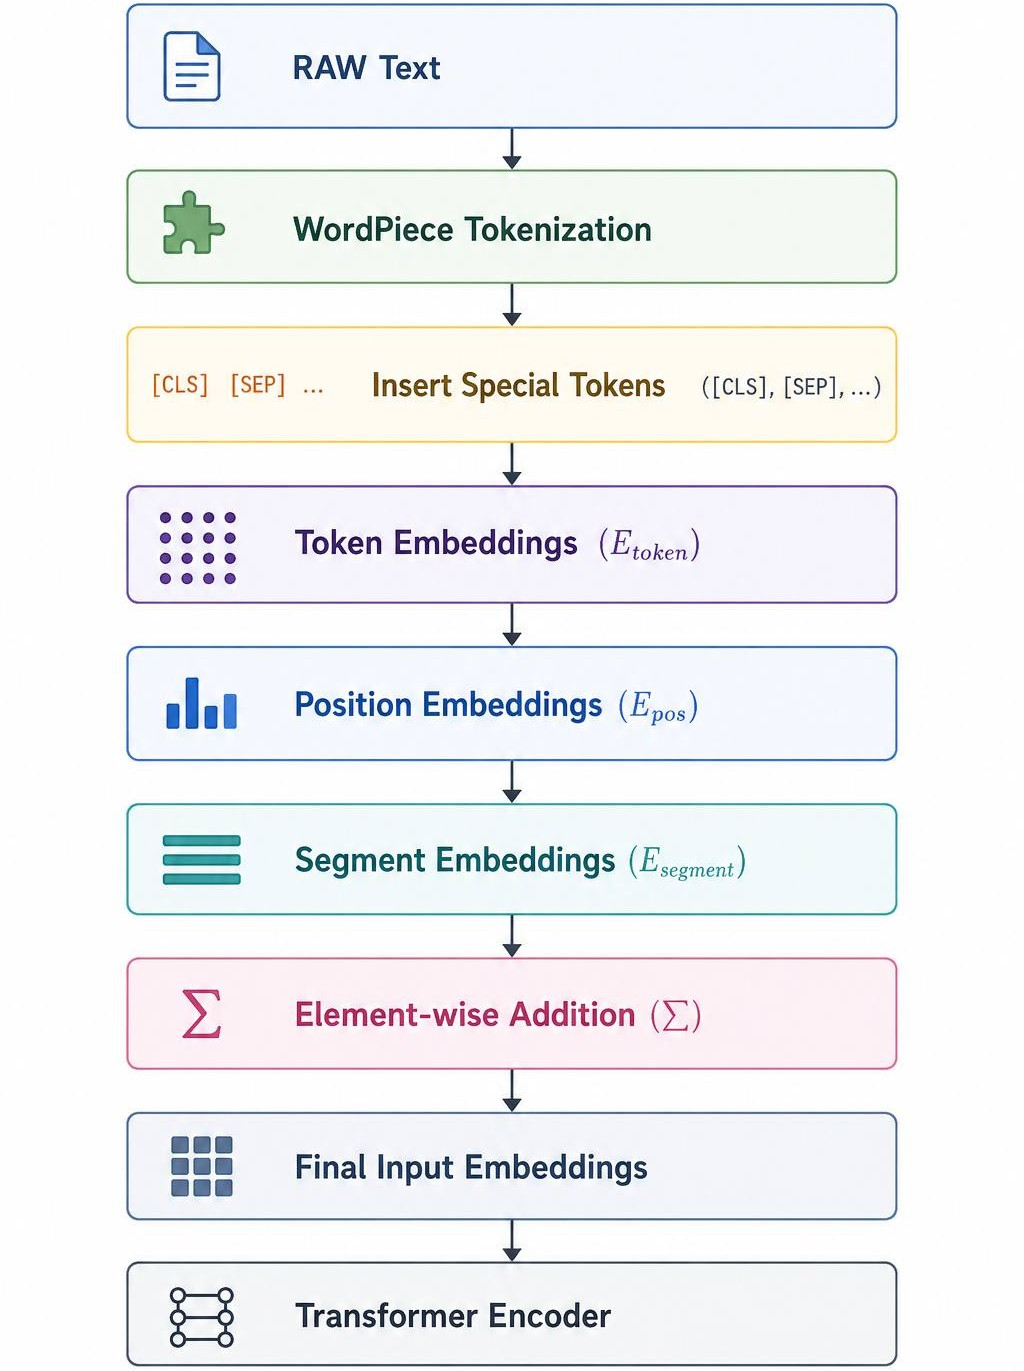
\includegraphics[width=0.95\textwidth]{figures/rnn1.jpg}
\end{figure}

\clearpage
\subsection{Bidirectional Learning}

The defining characteristic of BERT is its ability to learn bidirectional contextual representations. Unlike autoregressive language models, which process text from left to right, BERT simultaneously attends to both the left and right context of every token. This enables the model to construct richer semantic representations and achieve strong performance on language-understanding tasks.

Traditional autoregressive models predict the next token by Considering only the Previous tokens. In Contrast, BERT Processes the entire Sequence simultaneously. Every token can attend to every other token in The Sentence.

\subsection{Next Sentence Prediction (NSP)}

\paragraph{Motivation} Many NLP tasks require understanding the relationship between two sentences rather than a single sentence. Examples include question answering, natural language inference, and semantic similarity.

To Capture These inter-Sentence relationships, BERT introduces Next Sentence Prediction (NSP) as a Second Pretraining Objective.

\paragraph{Training Data Construction}
During Pretraining, The model receives pairs of Sentences.
\begin{itemize}
    \item $50\%$ of The pairs Contain two consecutive sentences from The Original Corpus ($\text{IsNext}$)
    \item $50\%$ Contain two randomly selected, unrelated sentences ($\text{NotNext}$). This creates a balanced binary classification problem.
\end{itemize}

This Creates a balanced binary Classification Problem.

\paragraph{Classification}
After passing through the encoder, the contextual representation of the \texttt{[CLS]} token, $h_{\text{cls}}$, is used as a representation of the entire sentence pair. A linear classifier predicts whether sentence B follows sentence A:
\begin{equation}
P(y) = \text{Softmax}(h_{\text{cls}} W + b)
\end{equation}

\paragraph{Loss function}
NSP is optimized using binary cross-entropy loss:
\begin{equation}
\mathcal{L}_{\text{NSP}} = -y \log(p) - (1-y) \log(1-p)
\end{equation}
\begin{itemize}
    \item $y=1$: for $\text{IsNext}$
    \item $y=0$: for $\text{NotNext}$
\end{itemize}

BERT is trained by optimizing both objectives simultaneously:
\begin{equation}
\mathcal{L} = \mathcal{L}_{\text{MLM}} + \mathcal{L}_{\text{NSP}}
\end{equation}
The encoder parameters are updated jointly using the combined loss.

\subsection{Limitations of NSP}

Subsequent research found that NSP contributed less than initially expected.

The RoBERTa model removed NSP entirely and achieved better performance by training longer on larger datasets.

Although NSP is no longer widely used in modern encoder models, it remains an important component of the original BERT architecture.

Thus, BERT learns both contextual word representations and sentence-level semantics. Although later models demonstrated that NSP is not essential, it played a significant role in the original BERT training procedure.

\subsection{Pretraining Summary}

Before BERT can be applied to downstream tasks such as sentiment analysis and question answering, it undergoes a large-scale pretraining phase. During this stage, the model learns general linguistic knowledge from massive collections of unlabeled text using the self-supervised objectives introduced in MLM (masked language modeling) and NSP (next-sentence prediction).

The result of pretraining is a model that captures grammar, semantics, contextual relationships, and sentence-level information, making it an effective starting point for many NLP applications.

\subsection{Fine-Tuning BERT}

Because BERT has already learned general language representations during pretraining, only a small amount of additional training is needed to specialize these representations for a specific task.

Rather than learning language from scratch, the model learns how to map its existing knowledge to the desired outputs.

Fine-tuning adapts a pretrained BERT model to a specific downstream task using labeled data. During training, both the encoder and the prediction head are optimized jointly, allowing the model to specialize its contextual representations while retaining the linguistic knowledge acquired during pretraining. This transfer-learning approach is one of the main reasons for BERT's effectiveness across a wide range of NLP tasks.

\paragraph{Fine-Tuning Pipeline}
The standard procedure for fine-tuning BERT on downstream tasks is illustrated below:
\begin{figure}[H]
    \centering
    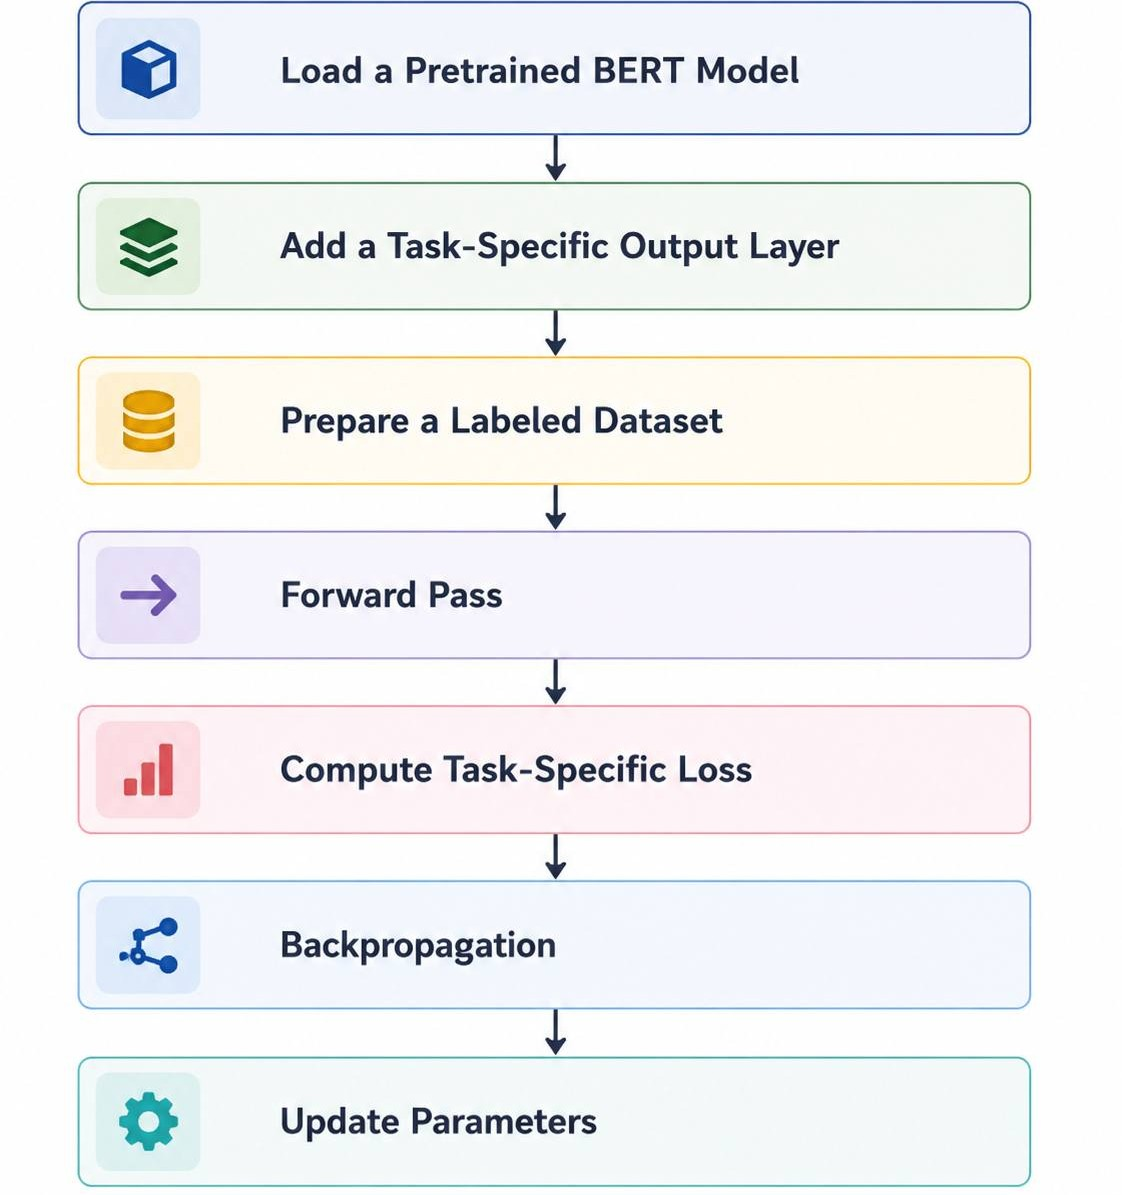
\includegraphics[width=0.95\textwidth]{figures/rnn2.jpg}
\end{figure}
\section{Decoder-Only Transformers (GPT Family)}

The decoder-only architecture emerged from the observation that many applications require only text generation or next-token prediction. The encoder becomes unnecessary, allowing the model to rely solely on the Transformer decoder. This simplification led to the GPT family of models, which has become the dominant architecture for modern large language models because of its scalability, simplicity, and effectiveness in autoregressive text generation.

\subsection{The Limitations of the Original Transformer}

Consider the task of machine Translation:
\begin{equation*}
\text{English} \longrightarrow \text{Encoder} \longrightarrow \text{Context Representation} \longrightarrow \text{Decoder} \longrightarrow \text{French}
\end{equation*}

The decoder requires the encoder because it must generate a sentence based on another input sentence.

Now consider a LLM such as ChatGPT:
\begin{itemize}
    \item Input: Explain what a Transformer is
    \item Desired output: A Transformer is a neural network architecture\dots
\end{itemize}

The model does not transform one sequence into another independent sequence. Instead, it continues the text that already exists: prompt plus generated tokens. No separate encoder source sentence is required.

Because generation depends only on previously generated tokens, the encoder becomes unnecessary.
\begin{itemize}
    \item Since no separate input sequence needs to be encoded, the entire encoder stack can be removed.
    \item The decoder alone is sufficient because it already contains masked self-attention, allowing it to process previously generated tokens while preventing access to future tokens.
\end{itemize}

\subsection{Birth of GPT}

In 2018, OpenAI introduced GPT (Generative Pre-trained Transformer). Unlike BERT, which retained only the encoder, GPT retained only the decoder. Its architecture can be summarized as:
\begin{align*}
\text{Input Token} &\longrightarrow \text{Token Embedding, Positional Embedding} \\
&\longrightarrow \text{Stack of Transformer Decoders} \\
&\longrightarrow \text{Linear Projection} \longrightarrow \text{Softmax} \longrightarrow \text{Next Token Probability}
\end{align*}

The model is trained to repeatedly predict the next token in a sequence using autoregressive language modeling.

The GPT architecture is obtained by simplifying the original Transformer decoder. Since language modeling requires only a single sequence, the encoder is removed, eliminating the need for encoder-decoder (cross-)attention. As a result, queries, keys, and values are all computed from the decoder's hidden representations, leaving masked multi-head self-attention as the only attention mechanism. This simplification reduces computational complexity while preserving the model's ability to generate text autoregressively.

\subsection{Cross Attention Key, Value, Query}

The decoder contains a cross-attention layer that allows it to access the encoder output while generating each token in encoder-decoder Transformers. Queries are computed from the decoder hidden states, whereas keys and values are computed from encoder representations. This enables the decoder to retrieve relevant information from the source sequence throughout generation.

Cross-attention is therefore essential for sequence-to-sequence tasks such as machine translation, where the decoder must continuously reference the encoder input sentence. The main question is: what happens to cross-attention when the encoder is removed in GPT?

GPT is not a sequence-to-sequence model. GPT performs language modeling, where the prompt and generated text belong to the same sequence. Once cross-attention is removed, the only remaining attention mechanism is masked multi-head self-attention. All three matrices are now computed from the decoder hidden states:
\begin{align*}
Q &= X W_Q \\
K &= X W_K \\
V &= X W_V
\end{align*}

Thus, GPT performs self-attention only. Every token attends to previous tokens within the same sequence.

\subsection{The New Decoder Block}

After removing cross-attention, each GPT block contains only two computational sublayers:
\begin{figure}[H]
    \centering
    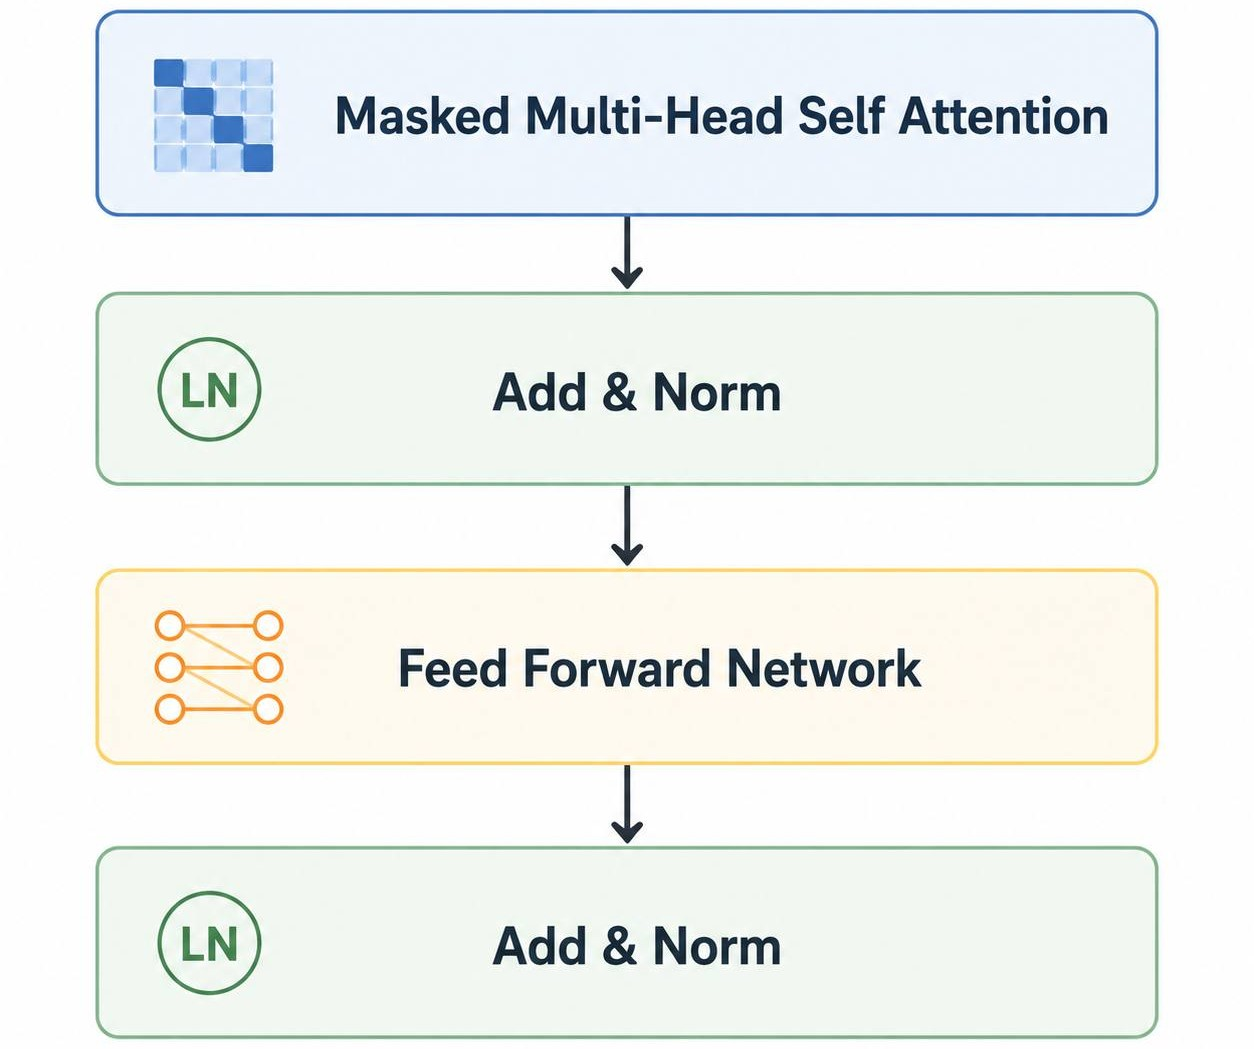
\includegraphics[width=0.95\textwidth]{figures/rnn3.jpg}
\end{figure}


This architecture is considerably simpler than The Original Transformer decoder while Preserving everything required for Autoregressive generation.

At first removing Cross-Attention might Seem like a loss of information. However, GPT does not require information from another Sequence. The Prompt itself becomes part of the decoder input, the Prompt itself provides the Context that would otherwise have been supplied by an encoder.

\subsection{GPT Input Architecture}

GPT converts raw text into numerical representations through tokenization, Vocabulary lookup, token embedding, and positional embedding:
\begin{equation}
E = E_{\text{pos}} + E_{\text{TokenEmb}}
\end{equation}
Unlike BERT, GPT uses only Token and Positional embedding because it Processes a single autoregressive sequence, while early GPT models relied on learnable absolute pos embedding, modern decoder-only models predominantly use Rotary Pos Embedding (RoPE) to Support long-context reasoning and improved positional Generalization.

\subsection{Training GPT}

Unlike traditional supervised learning, GPT does not Require labeled datasets. Instead, the model is trained On large text corpora Collected from sources such as: Books, wikipedia, Scientific Articles, News websites...

Through extensive Optimization over billions to trillions of Tokens, The Model learns General language representations, factual Knowledge, reasoning patterns, and Coding abilities. The resulting foundation model serves as The starting point for subsequent stages such as supervised fine-tuning\dots

\paragraph{Inference}
Autoregressive Generation is The inference Procedure used by GPT and other decoder-only language models. Starting from an input Prompt, The model predicts The one Token at a time, appends it to The Sequence, and repeats The Process until a stopping Condition is reached. Because each prediction depends on all previous tokens, inference is inherently Sequential. Efficient Generation relies on The KV cache.

\subsection{Decoding Algorithms}

After GPT computes The Probability distribution over the Vocabulary, it must choose which token to Generate next. This decision is performed by a decoding algorithm.

\paragraph{Greedy Search}
Always selects The Token with the highest probability. \\
\textit{Limitation:}
\begin{itemize}
    \item Often Produces repetitive Text
    \item Can miss better Overall Sequence
    \item Limited diversity
\end{itemize}

\paragraph{Beam Search}
Maintains the top-$k$ most probable partial Sequences. \\
\textit{Limitation:}
\begin{itemize}
    \item Computationally expensive
    \item Often Generates generic Response
    \item Rarely used in modern LLMs
\end{itemize}

\paragraph{Temperature Sampling}
Control the sharpness of The probability distribution before Softmax:
\begin{itemize}
    \item $0.2 - 0.5$: Factual tasks
    \item $0.7 - 1.0$: Balanced Generation
    \item $+1.2$: Highly Creative generation
\end{itemize}

\paragraph{Top-$K$ Sampling}
Instead of Considering the entire vocabulary, Top-$K$ sampling Keeps only the $K$ most probable tokens. The Remaining tokens receive probability 0, then performed only among these top-$K$ candidates.

\paragraph{Top-$P$ (Nucleus) Sampling}
Instead of Selecting a fixed number of Tokens, Top-$P$ Sampling selects The smallest set of tokens whose cumulative probability exceeds $p$. The candidate set changes dynamically depending On the probability distribution.

\paragraph{Typical Sampling}
Selects tokens whose information content is close to The expected entropy of the Probability distribution, it Prefers tokens that are statistically typical for The Current context.

\paragraph{Repetition Penalty}
During long generation, language models may Repeat words or phrases. A repetition penalty decrease the Probability of tokens that have already appeared in the Generated sequence. This encourages more varied and Coherent Outputs.

\subsection{Combined Decoding Strategies}

Most modern LLMs use a Combination of Decoding techniques rather than a Single algorithm. A Common Combination:
\begin{itemize}
    \item Temperature Sampling
    \item Top-$P$ Sampling
    \item Repetition Penalty
\end{itemize}

This combination provides a good balance between factual accuracy, fluency, and diversity.

\subsection{Best Decoder-Only Models}
\begin{itemize}
    \item ChatGPT
    \item DeepSeek
    \item Claude
    \item LLaMA
    \item Qwen
    \item Grok
\end{itemize}


\chapter{Vision Transformers (ViT)}

\section{Why CNNs Are Not Enough}

Since the introduction of AlexNet in 2012, CNNs have been the dominant architecture for computer vision. Despite their success, CNNs possess inherent architectural limitations. Their reliance on local convolutional operations makes modeling long-range dependencies difficult and often requires increasingly deep networks to capture global context.

These limitations motivated researchers to investigate whether the Transformer architecture, which had already revolutionized Natural Language Processing, could also replace CNNs in computer vision.

Many visual recognition tasks require understanding interactions between objects that are spatially far apart. A local convolution cannot directly relate two distant image regions; instead, information must propagate gradually through multiple convolution layers. Consequently, capturing global context becomes increasingly difficult as image size grows.

\subsection{Motivation for Vision Transformers (ViT)}

The Vision Transformer was designed around a simple question:
\begin{center}
\textbf{Can an image be treated like a sentence?}
\end{center}

The key insight behind ViT was that an image can also be represented as a sequence by dividing it into small patches.

Once converted into a sequence of patches, the standard Transformer encoder can process the image without using any convolutional layers. This idea became the foundation of modern Vision Transformers.

\subsubsection*{Advantages}
\begin{itemize}
    \item Direct modeling of long-range dependencies.
    \item Global receptive field from the first attention layer.
    \item Greater flexibility with larger datasets and models.
    \item Better scalability due to weaker inductive bias.
    \item Unified architecture for both language and vision.
\end{itemize}

However, these benefits come at the cost of increasing data requirements and higher computational complexity, motivating later improvements such as DeiT, Swin Transformer, and Masked Autoencoders.


\section{Image to Sequence}

The key idea of the ViT is to divide the image into fixed-size patches and treat each patch as a token, just as words are treated as tokens in NLP.

Instead of processing individual pixels, ViT divides the image into non-overlapping square patches.
\begin{figure}[H]
\centering
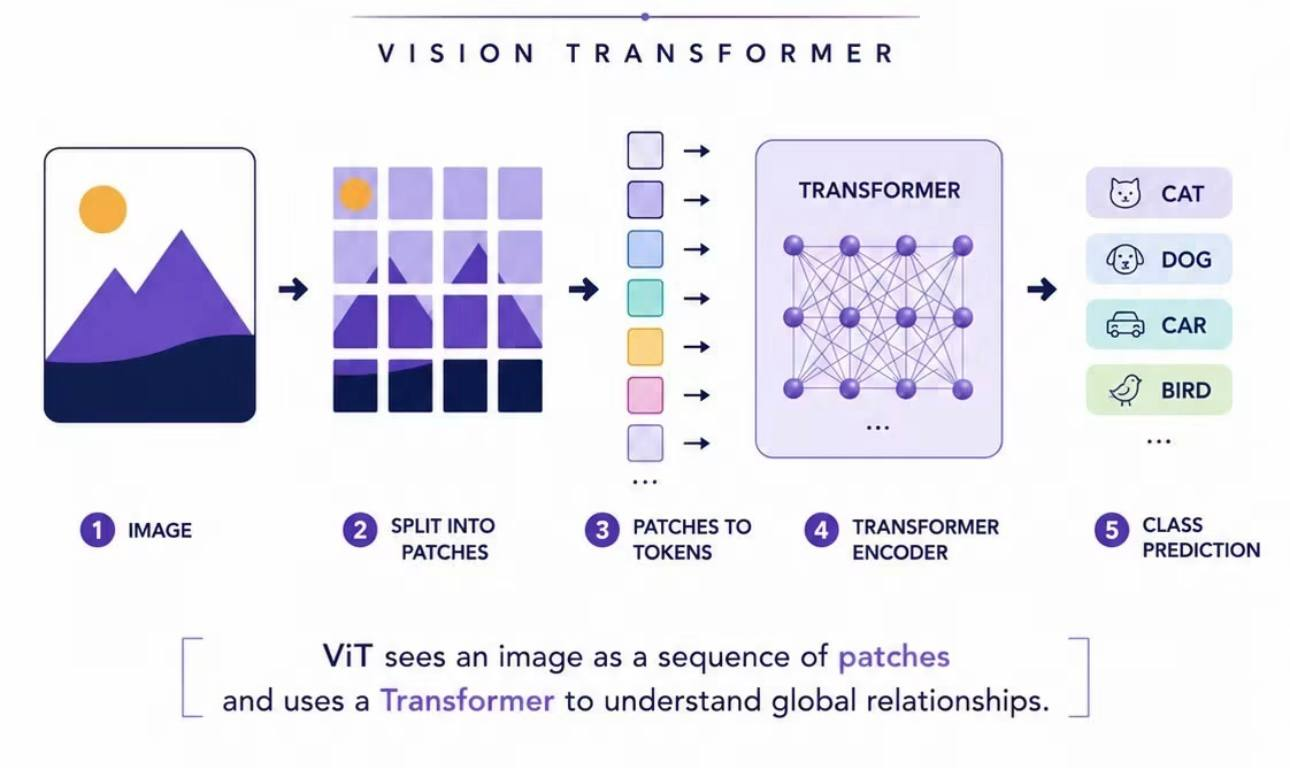
\includegraphics[width=0.95\textwidth]{figures/vit patches.jpg}
\end{figure}
\begin{itemize}
    \item \textbf{Image Size}: $224 \times 224 \times 3$
    \item \textbf{Patch Size}: $16 \times 16$: The image is divided into small $16 \times 16$ RGB patches.
\end{itemize}

\subsection{Number of Patches}
\[
N = \frac{H}{P} \times \frac{W}{P} \implies N = \frac{224}{16} \times \frac{224}{16} = 14 \times 14 = 196
\]

\subsection{Flattening Each Patch}
Each patch still has three dimensions ($16 \times 16 \times 3$). Before being processed by the Transformer, each patch is flattened into a one-dimensional vector:
\[
16 \times 16 \times 3 = 768
\]
Every patch is now represented by a vector containing 768 values.

After flattening all patches, the original image is transformed into a sequence. The resulting tensor is $196 \times 768$. Instead of a 2D image, the Transformer now receives a sequence of 196 vectors.


\section{Patch Embedding}

After dividing the image into patches, each patch is represented as a flattened vector. However, these vectors cannot be fed directly into the Transformer because the Transformer expects every input token to have the same embedding dimension $d_{\text{model}}$.

Therefore, each flattened patch is projected to a fixed-dimension embedding space using a learnable linear layer. This process is called \textbf{Patch Embedding}.

The Transformer expects embeddings of dimension $d_{\text{model}}$, for example:
\begin{itemize}
    \item \textbf{ViT-Base}: $d_{\text{model}} = 768$
    \item \textbf{ViT-Large}: $d_{\text{model}} = 1024$
    \item \textbf{ViT-Huge}: $d_{\text{model}} = 1280$
\end{itemize}

Therefore, every patch must be transformed into a vector of size $d_{\text{model}}$.


\section{Positional Embedding}

After patch embedding, Vision Transformers add learnable positional embeddings to preserve the spatial arrangement of image patches.

Unlike the original Transformer (2017) which used fixed sinusoidal positional encodings, ViT uses learnable positional embeddings:
\[
E_{\text{pos}} \in \mathbb{R}^{(N+1) \times d_{\text{model}}}
\]
\begin{itemize}
    \item $N =$ Number of image patches
    \item $+1 =$ The CLS token
    \item $d_{\text{model}} =$ Embedding dimension
\end{itemize}

Each position has its own learnable vector. These vectors are initialized randomly and optimized during training.

\subsection{Adding Positional Embeddings}
\[
X = E_{\text{patch}} + E_{\text{pos}}
\]
Each patch embedding now contains:
\begin{itemize}
    \item Visual information.
    \item Spatial position.
\end{itemize}

\subsection{Why Add the CLS Token First?}

The CLS token is treated like an additional patch. Therefore, it also requires positional information. For this reason, the CLS token is first appended to the patch sequence, and then positional embeddings are added to all tokens simultaneously. This ensures that the CLS token has its own learnable positional embedding.


\section{CLS Token}

Unlike NLP, where the output may consist of multiple tokens, image classification requires only one prediction for the entire image.

The Vision Transformer solves this problem by introducing a special learnable token called the \textbf{CLS (Classification) Token}.

Instead of representing a single image patch, the CLS token is designed to collect information from all image patches through self-attention. After passing through all Transformer encoder layers, it serves as a compact representation of the entire image and is used for classification.

Before entering the Transformer encoder, a learnable CLS token is prepended to the sequence of patch embeddings:
\[
\text{If patch embeddings are } [P_1, P_2, \dots, P_N]
\]
\[
\text{The input sequence becomes } [\text{CLS}, P_1, P_2, \dots, P_N]
\]
\[
196 \times 768 \longrightarrow 197 \times 768
\]
\[
\text{CLS} \in \mathbb{R}^{d_{\text{model}}}
\]

Initially, it contains random values, but during training it learns how to gather the most useful information for the target task.

During every attention layer:
\begin{itemize}
    \item The CLS token attends to every image patch.
    \item Every image patch can also attend to the CLS token.
\end{itemize}

By the end of the encoder, the CLS token becomes a global representation of the image.


\section{Classification Head}

After the final encoder layer, only the CLS token is used for image classification.

The CLS embedding is passed through a linear classification head:
\[
y = \text{CLS} \cdot W + b
\]
The resulting logits are converted into class probabilities using Softmax.

The CLS token provides several advantages:
\begin{itemize}
    \item Produces a single representation for the entire image.
    \item Learns which regions are most important through attention.
    \item Keeps the architecture simple.
    \item Can be reused for downstream tasks after fine-tuning.
\end{itemize}

\section{Vision Transformer (ViT) Architecture}

Vision Transformer (ViT), proposed by Google Research in 2020, was the first architecture to successfully apply the standard Transformer encoder directly to image classification.

Unlike CNNs, which rely on convolutional layers to extract features, ViT processes an image as a sequence of patches and uses only Transformer encoder blocks to learn visual representations. The central idea is simple: \textbf{An image can be treated like a sentence, where each image patch is equivalent to a word (token).}

\begin{figure}[H]
    \centering
    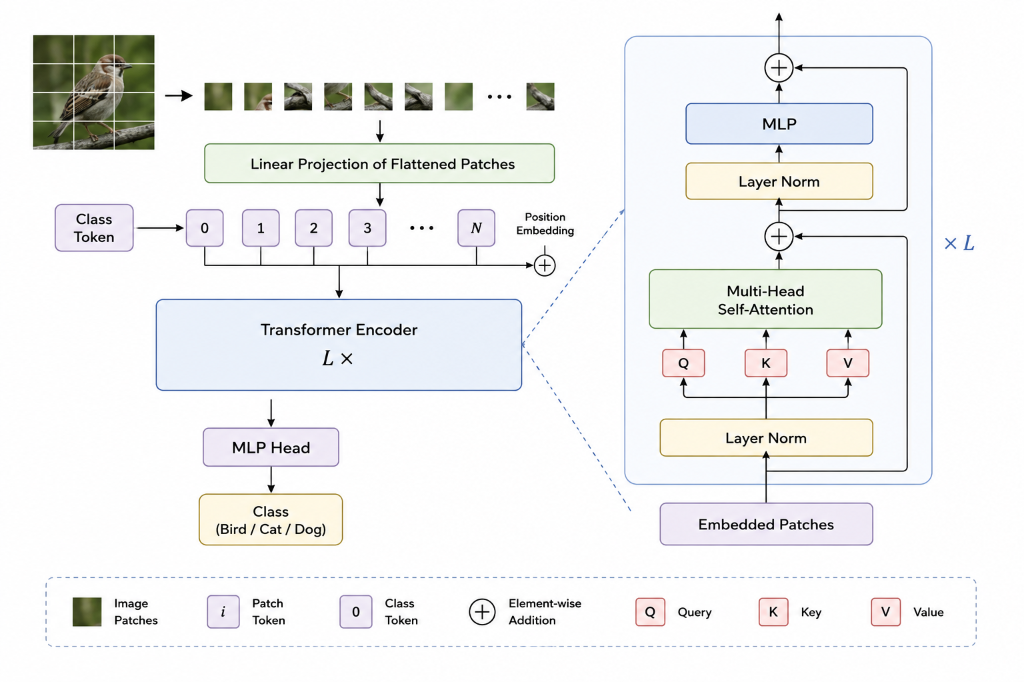
\includegraphics[width=0.92\linewidth]{figures/fig_6_vit.png}
    \caption{Vision Transformer (ViT) Architecture.}
    \label{fig:vit_architecture}
\end{figure}



The most common Vision Transformers are:
\begin{center}
\begin{tabular}{lcc}
\hline
\textbf{Model} & \textbf{Encoder Blocks} & \textbf{Parameters} \\
\hline
ViT-Base & 12 & 86 M \\
ViT-Large & 24 & 307 M \\
ViT-Huge & 32 & 632 M \\
\hline
\end{tabular}
\end{center}

\subsection{Limitations of ViT}
\begin{itemize}
    \item Requires very large training datasets.
    \item Higher computational cost than CNNs.
    \item Quadratic attention complexity ($\mathcal{O}(N^2)$).
    \item Less data-efficient because it lacks CNN inductive bias.
\end{itemize}

These limitations motivated several improved architectures including:
\begin{itemize}
    \item \textbf{DeiT}: More data-efficient training.
    \item \textbf{Swin Transformer}: Linear attention complexity.
    \item \textbf{MAE}: Self-supervised pretraining.
\end{itemize}

Vision Transformers have very weak inductive biases. They must learn spatial relationships directly from data, which requires much larger datasets and more computational resources. The original ViT paper demonstrated that training directly on ImageNet-1K (1.3 million images) was not sufficient to outperform state-of-the-art CNNs.

Instead, pretrained ViT on much larger datasets before fine-tuning on ImageNet. The largest datasets used included:
\begin{itemize}
    \item \textbf{ImageNet-21K}: $\sim 14$ million images, 21,000 classes.
    \item \textbf{JFT-300M}: $\sim 300$ million images, proprietary Google dataset.
\end{itemize}

Pretraining on these massive datasets allowed ViT to learn rich visual representations.

After large-scale pretraining, the model is adapted to a specific downstream task through fine-tuning. Typically, only the final classification layer is replaced to match the number of classes in the new dataset, while the pretrained encoder weights are reused and further optimized.


\section{DeiT (Data-efficient Image Transformer)}

One of the biggest criticisms of the original Vision Transformer was that it required hundreds of millions of training images to outperform CNNs. This made ViT impractical for most researchers and companies.

In 2021, Facebook AI introduced DeiT, demonstrating that Vision Transformers could be trained using only ImageNet while achieving competitive performance. The key innovation was \textbf{Knowledge Distillation} adapted specifically for Vision Transformers.

\subsection{The Problem with ViT}
\begin{itemize}
    \item Very large datasets.
    \item Extremely long training.
    \item Huge computational resources.
\end{itemize}

Without massive pretraining, CNNs like ResNet generally performed better. The challenge was therefore: \textbf{Can a Vision Transformer learn efficiently from a relatively small dataset?} DeiT answered \textbf{yes}.

\subsection{Main Contributions of DeiT}

DeiT introduced three major improvements:
\begin{enumerate}
    \item Efficient training recipe.
    \item Strong data augmentation and regularization.
    \item Knowledge distillation using a Distillation Token.
\end{enumerate}

\subsection{Knowledge Distillation}

Knowledge distillation is a technique where a large pretrained model (\textbf{Teacher}) transfers knowledge to a smaller model (\textbf{Student}). Instead of learning only from the ground-truth labels, the student also learns from the predictions of the teacher.

CNNs already learn excellent visual features from relatively small datasets. Instead of discarding decades of CNN research, DeiT leverages CNN knowledge to train the Transformer more effectively.

\subsection{Distillation Token}

DeiT adds another learnable token:
\[
[\text{CLS}, \text{DIST}, P_1, P_2, \dots, P_N]
\]

The input sequence now contains:
\begin{itemize}
    \item CLS Token
    \item DIST Token
    \item Image patches
\end{itemize}

During self-attention, the distillation token interacts with all image patches, just like the CLS token. However, instead of learning from the ground-truth labels, it learns to mimic the teacher model's prediction.

Thus:
\begin{itemize}
    \item \textbf{CLS Token} $\rightarrow$ Supervised by true labels.
    \item \textbf{DIST Token} $\rightarrow$ Supervised by teacher network.
\end{itemize}

The Transformer therefore learns from both supervision signals simultaneously.

\begin{figure}[H]
    \centering
    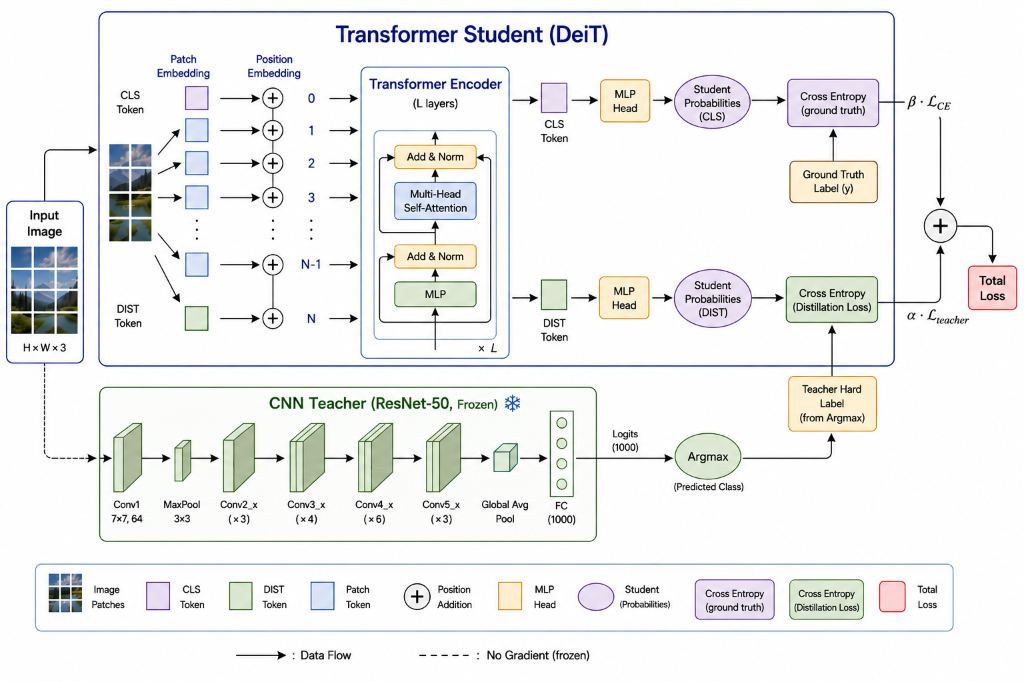
\includegraphics[width=0.92\linewidth]{figures/fig_6_deit.png}
    \caption{Transformer Student (DeiT) \& CNN Teacher (ResNet-50) Knowledge Distillation Architecture.}
    \label{fig:deit_architecture}
\end{figure}

\subsection{Inference}

After training, the teacher network is discarded. Only the DeiT model is used for inference. The teacher is needed only during training.

\subsection{Advantages (Compared to ViT)}
\begin{itemize}
    \item Much smaller training datasets.
    \item Faster convergence.
    \item Better data efficiency.
    \item Competitive performance on ImageNet-1K.
    \item No need for massive proprietary datasets.
\end{itemize}


\section{Swin Transformer (Shifted Window Transformer)}

Although the original Vision Transformer (ViT) achieved excellent accuracy, it had a major limitation: Self-attention has quadratic complexity $\mathcal{O}(N^2)$, where $N$ is the number of image patches.

As image resolution increases, the number of patches increases, making computation and memory requirements extremely expensive.

To solve this problem, Microsoft introduced the Swin Transformer in 2021. Its two main innovations are:
\begin{itemize}
    \item \textbf{Window-based Multi-head Self-Attention (W-MSA)}
    \item \textbf{Shifted Window Multi-head Self-Attention (SW-MSA)}
\end{itemize}

These ideas greatly reduce computation while still allowing information to flow across the entire image.

\subsection{Window Attention (W-MSA)}

Instead of allowing every patch to attend to every other patch, Swin divides the image into small non-overlapping windows.

\begin{figure}[H]
    \centering
    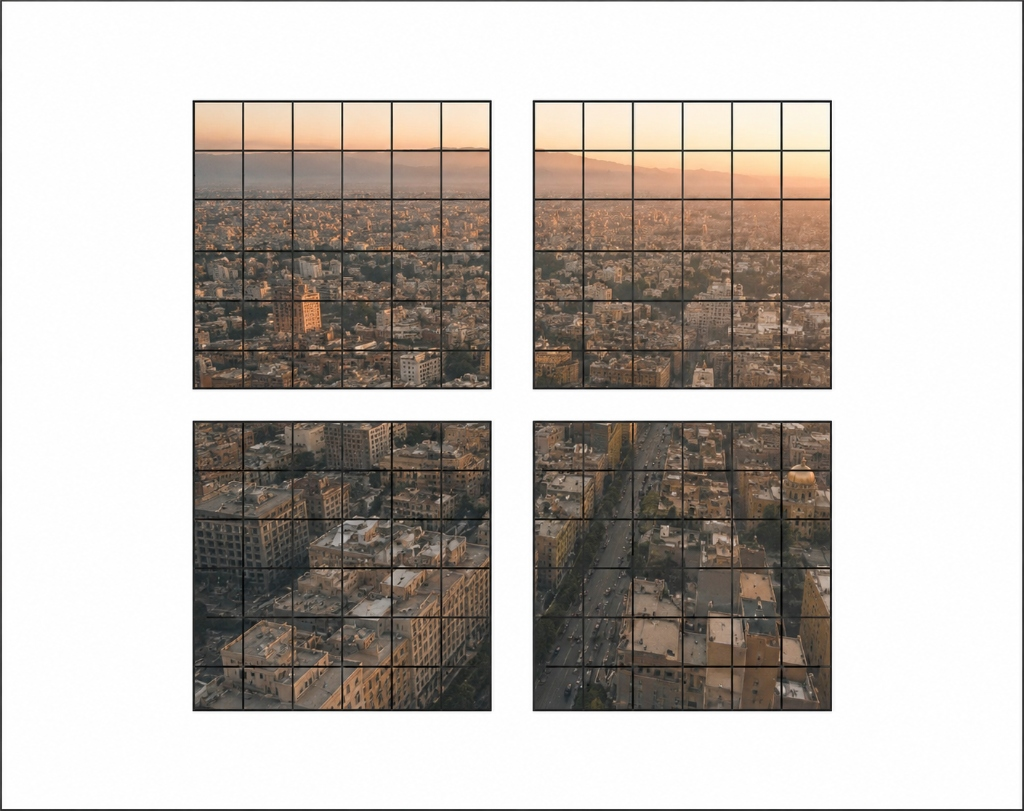
\includegraphics[width=0.75\linewidth]{figures/fig_6_swin_window_partition.jpg}
    \caption{Window Partitioning in Swin Transformer (W-MSA).}
    \label{fig:swin_window_partition}
\end{figure}

Each square window is processed independently. Inside one window, every patch attends only to patches within the same window. No attention is computed between different windows.

\subsubsection*{Computational Advantage}
Suppose Total patches $= 196$, window size $= 7 \times 7$ patches. Each window contains 49 patches. Instead of computing $196 \times 196$, each attention matrix becomes $49 \times 49$. This dramatically reduces computation. Instead of one huge attention matrix, the model computes several much smaller attention matrices.

However, it introduces a new issue:
\begin{center}
\textbf{Problem: Neighboring patches in different windows cannot communicate.}
\end{center}

\subsection{Shifted Window Attention (SW-MSA)}

This is Swin Transformer's key innovation. Instead of keeping the same window in every layer, the windows are shifted before the next attention operation.

\begin{figure}[H]
    \centering
    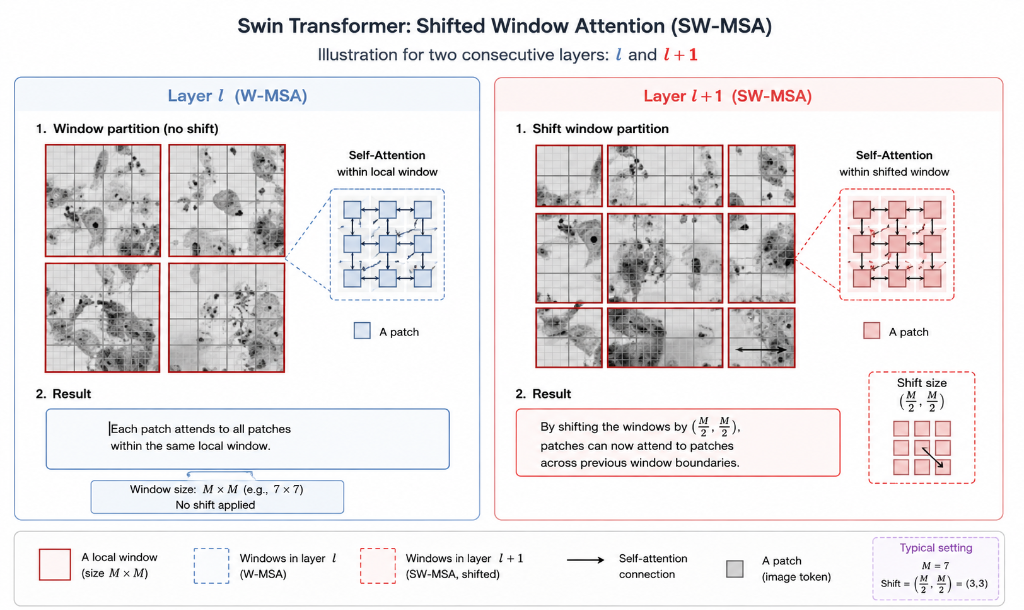
\includegraphics[width=0.90\linewidth]{figures/fig_6_swin_swmsa.png}
    \caption{Swin Transformer: Shifted Window Attention (SW-MSA) Mechanism.}
    \label{fig:swin_swmsa}
\end{figure}

The windows move by approximately half the window size (if a window contains 4 patches, so $\frac{4}{2} = 2$, it moved by 2 patches).

Patches that were previously in different windows now become part of the same window. This allows information to propagate across the entire image over multiple layers.

The process alternates between:
\begin{itemize}
    \item Window Attention (W-MSA)
    \item Shifted Window Attention (SW-MSA)
\end{itemize}

After several layers, information gradually flows across neighboring windows until the model effectively captures global context. Thus, Swin achieves a balance between:
\begin{itemize}
    \item Local efficiency.
    \item Global information exchange.
\end{itemize}




\section{Swin Architecture}

\begin{figure}[H]
    \centering
    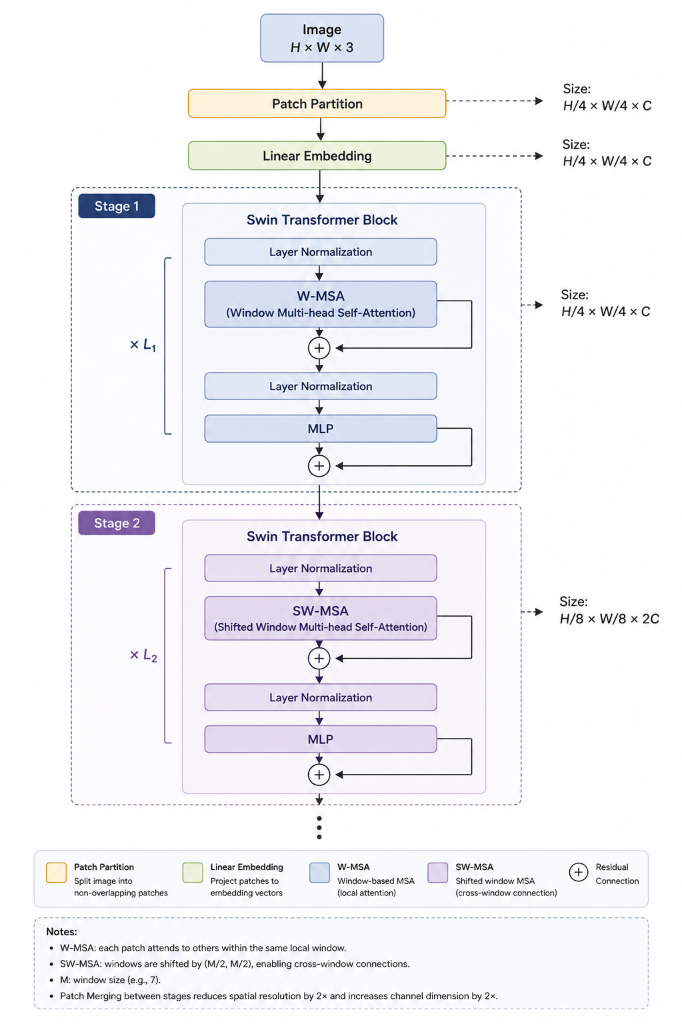
\includegraphics[width=0.88\linewidth]{figures/fig_6_swin_architecture.png}
    \caption{Swin Transformer Overall Architecture.}
    \label{fig:swin_architecture}
\end{figure}

\subsection{Two Successive Swin Transformer Blocks}

Each Stage contains Swin Transformer Blocks, and each Swin Transformer Block contains two successive Swin Transformer units (Block $l$ with W-MSA and Block $l+1$ with SW-MSA).



\begin{figure}[H]
    \centering
    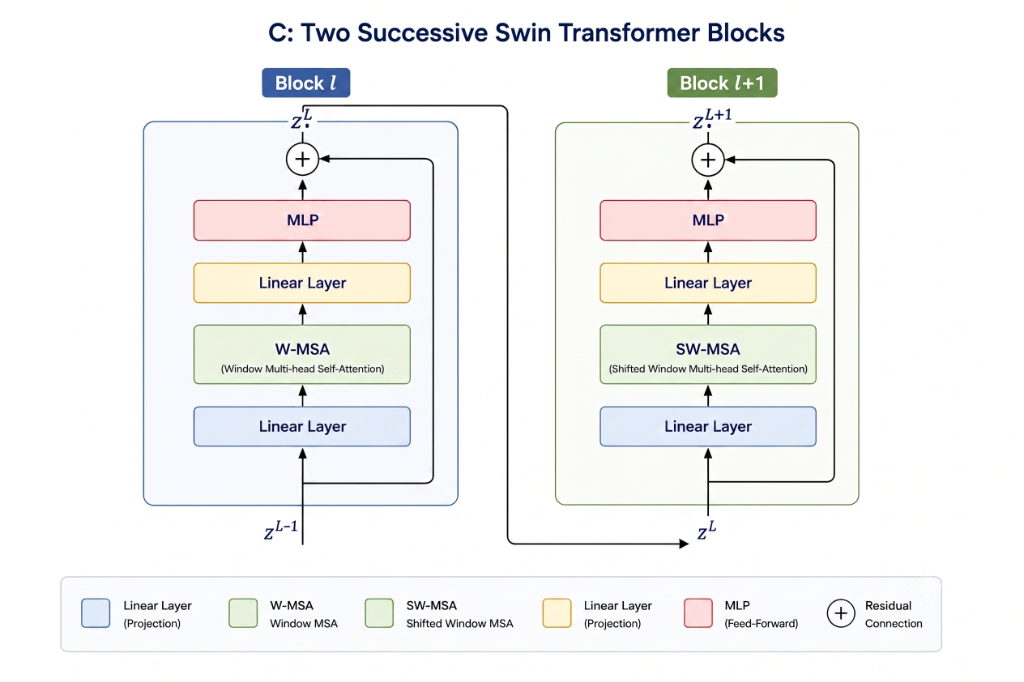
\includegraphics[width=0.82\linewidth]{figures/fig_6_swin_blocks.png}
    \caption{Two Successive Swin Transformer Blocks.}
    \label{fig:swin_blocks}
\end{figure}


\section{Summary}

\begin{itemize}
    \item The original ViT proved that Transformers could replace CNNs for image classification, but it remained computationally expensive for many vision tasks.
    \item Swin Transformer addressed this limitation by introducing window attention, shifted windows, and patch merging, making Transformers both efficient and scalable. These innovations allowed Swin to become one of the most widely adopted Transformer backbones in computer vision.
\end{itemize}

\chapter{Self-Supervised Learning}

\section{Motivation}

For many years, supervised learning dominated artificial intelligence because it achieved remarkable performance on tasks such as image classification, speech recognition, and machine translation. However, as deep learning models became larger, their demand for labeled data increased dramatically. Although billions of images and trillions of words are freely available on the Internet, only a small fraction of this data is manually labeled. Creating high-quality labels requires significant time, financial resources, and often the expertise of domain specialists, making supervised learning difficult to scale. This limitation motivated researchers to search for a new learning paradigm capable of exploiting the enormous amount of unlabeled data available while reducing the dependence on manual annotation.


\section{Why Not Simply Use Unsupervised Learning?}

Unsupervised learning had existed long before self-supervised learning, but its objective is fundamentally different. Traditional unsupervised methods focus on discovering hidden structures in data through clustering, dimensionality reduction, or density estimation. Although these techniques reveal patterns, they do not necessarily produce representations that are useful for tasks such as classification or detection. Researchers therefore sought a method that could learn discriminative representations while still avoiding manual labels.

Self-Supervised Learning (SSL) is a learning paradigm in which the supervision signal is generated automatically from the data itself, instead of relying on human annotations. The model creates its own prediction task, known as a pretext task, and learns meaningful representations by solving it. In this way, SSL combines the scalability of unsupervised learning with the representation quality of supervised learning.

\section{What Does SSL Actually Learn?}

Unlike supervised learning, whose immediate goal is to predict labels, SSL aims to learn representations. A representation is a feature vector (embedding) that captures the semantic information contained in the input. Once these representations are learned, they can be transferred to many downstream tasks such as classification, object detection, segmentation, retrieval, and medical image analysis.

Since unlabeled data is vastly more abundant than labeled data, self-supervised learning has become the preferred strategy for training modern foundation models. Today, many of the most influential AI systems---including \textbf{BERT}, \textbf{DINOv2}, \textbf{MAE}, and even \textbf{GPT} through next-token prediction---rely on self-supervised learning during pretraining.

\section{Pretext Tasks}

A pretext task is an artificial task created from the data itself.

\begin{table}[H]
\centering
\caption{Examples of Methods and Their Pretext Tasks}
\label{tab:pretext_tasks}
\begin{tabularx}{\textwidth}{lX}
\toprule
\textbf{Method} & \textbf{Pretext Task} \\
\midrule
\textbf{BERT} & Predict masked words \\
\textbf{MAE} & Reconstruct masked image patches \\
\textbf{SimCLR} & Match two augmented views \\
\textbf{DINO} & Match teacher-student representations \\
\bottomrule
\end{tabularx}
\end{table}

The model learns meaningful features while solving the pretext task. After SSL pretraining, the learned encoder is reused for real applications called downstream tasks, e.g., classification, object detection, face recognition. The SSL encoder is usually fine-tuned with a much smaller labeled dataset.

\section{The Two Main Families of SSL}

\begin{enumerate}[label=\Roman*)]
    \item \textbf{Contrastive Learning}: Learn by comparing representations.
    \begin{itemize}
        \item \textbf{SimCLR}
        \item \textbf{MoCo}
        \item \textbf{BYOL}
        \item \textbf{DINO}
    \end{itemize}
    
    \item \textbf{Masked / Reconstruction Learning}: Learn by reconstructing missing information.
    \begin{itemize}
        \item \textbf{BEiT}
        \item \textbf{MAE}
        \item \textbf{iBOT} (hybrid approach)
    \end{itemize}
\end{enumerate}

These two families dominate modern self-supervised vision research.

\section{Contrastive Learning}

The goal of S.S.L is to learn meaningful representations without labels. The question then becomes: can we tell the model which images are similar and which are different?

Contrastive learning solves this problem by creating its own supervision. Instead of learning from class labels, it learns by comparing different views of the data. The model is trained to bring representations of similar samples closer together while pushing representations of different samples farther apart in the embedding space.

\subsection{Positive Pairs}

A positive pair consists of two different views of the same sample. For example, given an image $x$, we apply two random augmentations:
\begin{itemize}
    \item Random Crop
    \item Color Jitter
    \item Gaussian Blur
    \item Horizontal Flip
\end{itemize}

Producing:
\begin{figure}[H]
\centering
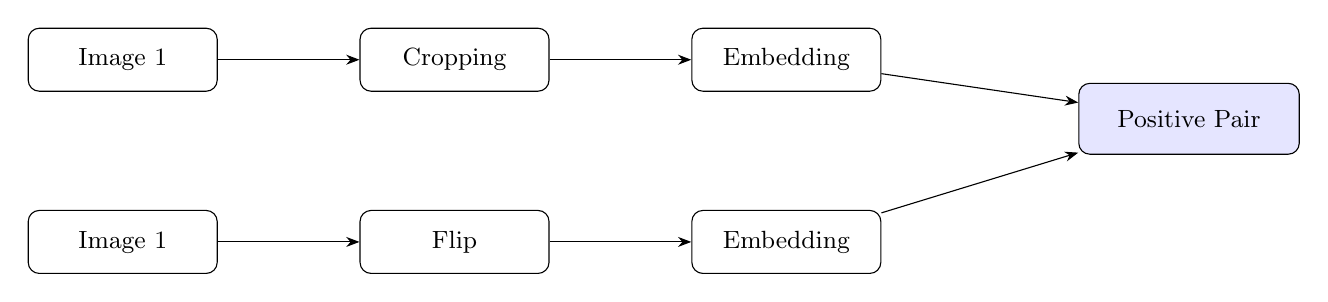
\begin{tikzpicture}[
node distance=1.8cm,
>=Stealth,
every node/.style={font=\small},
box/.style={draw, rounded corners, minimum width=2.4cm, minimum height=0.8cm, align=center},
pair/.style={draw, fill=blue!10, rounded corners, minimum width=2.8cm, minimum height=0.9cm}
]

% Top branch
\node[box] (img1) {Image 1};
\node[box, right=of img1] (crop) {Cropping};
\node[box, right=of crop] (emb1) {Embedding};

% Bottom branch
\node[box, below=1.5cm of img1] (img2) {Image 1};
\node[box, right=of img2] (flip) {Flip};
\node[box, right=of flip] (emb2) {Embedding};

% Pair
\node[pair, right=2.5cm of emb1, yshift=-0.75cm] (pair) {Positive Pair};

% Arrows
\draw[->] (img1) -- (crop);
\draw[->] (crop) -- (emb1);
\draw[->] (img2) -- (flip);
\draw[->] (flip) -- (emb2);

\draw[->] (emb1) -- (pair);
\draw[->] (emb2) -- (pair);

\end{tikzpicture}
\caption{Construction of a positive pair.}
\end{figure}

Although the two images look different, they originate from the same image and therefore form a positive pair. The model should produce similar embeddings for both views.

\subsection{Negative Pairs}

A negative pair consists of two views coming from different samples.
\begin{figure}[H]
\centering
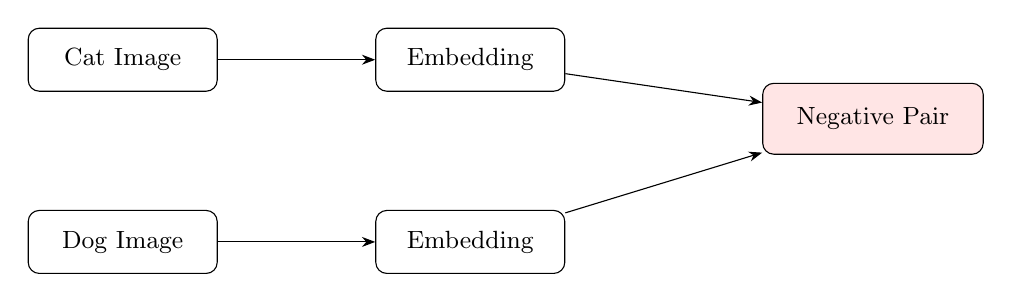
\begin{tikzpicture}[
node distance=2cm,
>=Stealth,
every node/.style={font=\small},
box/.style={draw, rounded corners, minimum width=2.4cm, minimum height=0.8cm, align=center},
pair/.style={draw, fill=red!10, rounded corners, minimum width=2.8cm, minimum height=0.9cm}
]

\node[box] (cat) {Cat Image};
\node[box, right=of cat] (emb1) {Embedding};

\node[box, below=1.5cm of cat] (dog) {Dog Image};
\node[box, right=of dog] (emb2) {Embedding};

\node[pair, right=2.5cm of emb1, yshift=-0.75cm] (pair) {Negative Pair};

\draw[->] (cat) -- (emb1);
\draw[->] (dog) -- (emb2);

\draw[->] (emb1) -- (pair);
\draw[->] (emb2) -- (pair);

\end{tikzpicture}
\caption{Construction of a negative pair.}
\end{figure}

Since the two images represent different objects, their embeddings should be separated in the embedding space.

The objective is therefore:
\begin{itemize}
    \item Positive pairs $\longrightarrow$ close together.
    \item Negative pairs $\longrightarrow$ far apart.
\end{itemize}

\begin{figure}[H]
    \centering
    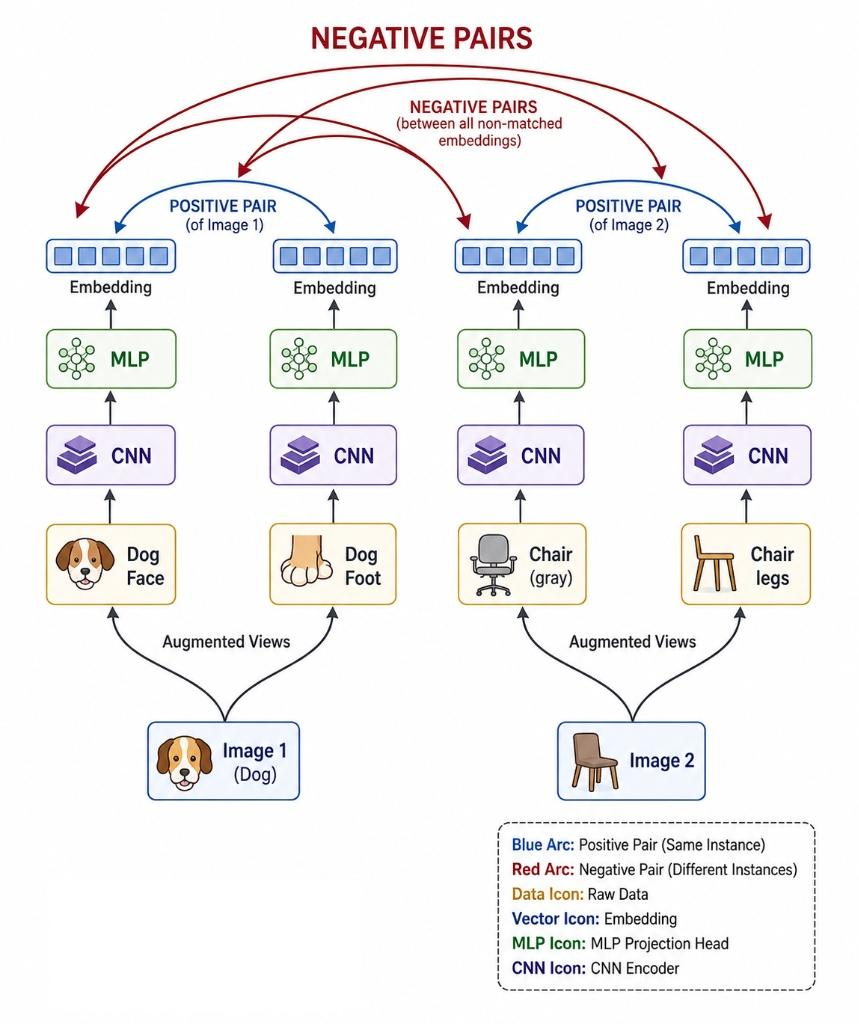
\includegraphics[width=0.92\textwidth]{figures/fig_7_contrastive_pairs.jpg}
    \caption{Contrastive Learning Framework with Positive and Negative Pairs.}
    \label{fig:contrastive_pairs}
\end{figure}

\section{Data Augmentation as Supervision}

In supervised learning, labels provide the supervision. In contrastive learning, data augmentation becomes the supervision.

By generating multiple views of the same image, the model automatically knows which samples should be considered similar, eliminating the need for manual annotations.

Common augmentations include:
\begin{itemize}
    \item Random Crop
    \item Random Resize
    \item Horizontal Flip
    \item Color Jitter
    \item Gaussian Blur
    \item Random Grayscale
\end{itemize}

The quality of these augmentations is one of the most important factors affecting S.S.L performance.

The model does not compare images directly; instead, it compares their embeddings.

The goal is to organize this space so that:
\begin{itemize}
    \item Similar images have nearby embeddings.
    \item Different images have distant embeddings.
\end{itemize}

To measure the similarity between two embeddings, contrastive learning typically uses cosine similarity:
\[
\text{Sim}(z_i, z_j) = \frac{z_i \cdot z_j}{\|z_i\| \cdot \|z_j\|}
\]
Most SSL methods normalize embeddings before computing cosine similarity.

\section{InfoNCE Loss}

The InfoNCE (Information Noise Contrastive Estimation) Loss is the objective function used in most contrastive learning methods. Its purpose is to learn an embedding space where positive pairs are close together and negative pairs are far apart.

For an anchor embedding $z_i$, a positive embedding $z_j$, and a set of negative embeddings, the InfoNCE Loss is:
\[
L_i = -\log \left( \frac{\exp\left( \frac{\text{sim}(z_i, z_j)}{\tau} \right)}{\sum_{k=1}^{K} \exp\left( \frac{\text{sim}(z_i, z_k)}{\tau} \right)} \right)
\]
where:
\begin{itemize}
    \item $z_i$: anchor embedding
    \item $z_j$: positive embedding
    \item $z_k$: all candidate embeddings (Positive + Negative)
    \item $\text{sim}$: cosine similarity
    \item $\tau$: temperature parameter
\end{itemize}

The numerator $\exp\left( \frac{\text{sim}(z_i, z_j)}{\tau} \right)$ contains the similarity between the anchor and its positive pair, which the model wants to maximize.

The denominator $\sum_{k} \exp\left( \frac{\text{sim}(z_i, z_k)}{\tau} \right)$ contains the similarity between the anchor and all candidate samples, including the positive and all negatives.

Minimizing the InfoNCE Loss therefore encourages the model to:
\begin{itemize}
    \item Increase the similarity between positive pairs.
    \item Decrease the similarity between negative pairs.
\end{itemize}

As training progresses, the embedding space becomes organized so that semantically similar samples are clustered together while dissimilar samples are separated.

\subsection{Temperature Parameter \texorpdfstring{($\tau$)}{(tau)}}

Before applying the Softmax in InfoNCE, similarities are divided by a temperature parameter ($\tau$): $\frac{\text{sim}(z_i, z_j)}{\tau}$. The temperature controls how strongly the model distinguishes between similar and dissimilar samples.
\begin{itemize}
    \item Small $\tau$: sharper probability distribution, stronger separation.
    \item Larger $\tau$: smoother distribution, weaker separation.
\end{itemize}

It is simply a hyperparameter used during training.

\subsection*{Summary}
Contrastive Learning enables self-supervised learning by comparing representations, instead of relying on labels. It creates positive pairs from different augmentations of the same sample and negative pairs from different samples. Images are mapped into an embedding space, where cosine similarity measures how close two embeddings are. The InfoNCE loss encourages positive pairs to become similar and negative pairs to become dissimilar, while the temperature parameter controls the sharpness of this optimization. These principles form the foundation of methods such as: \textbf{SimCLR}, \textbf{MoCo}, \textbf{BYOL}, and \textbf{DINO}.

\section{SimCLR (Simple Framework for Contrastive Learning of Visual Representations)}

Before \textbf{SimCLR}, contrastive learning methods often relied on complex architectures, memory banks, or specialized training procedures. In 2020, Google Research introduced \textbf{SimCLR}, demonstrating that a simple framework based on strong data augmentation, a projection head, and a contrastive loss could learn powerful visual representations without labels. \textbf{SimCLR} became the foundation for many later SSL methods.

The core idea of \textbf{SimCLR} is straightforward: generate two different augmented views of the same image, encode them into embeddings, and train the model to make these embeddings similar while separating them from embeddings of other images.

Thus, supervision comes entirely from the augmentations.

\begin{figure}[H]
    \centering
    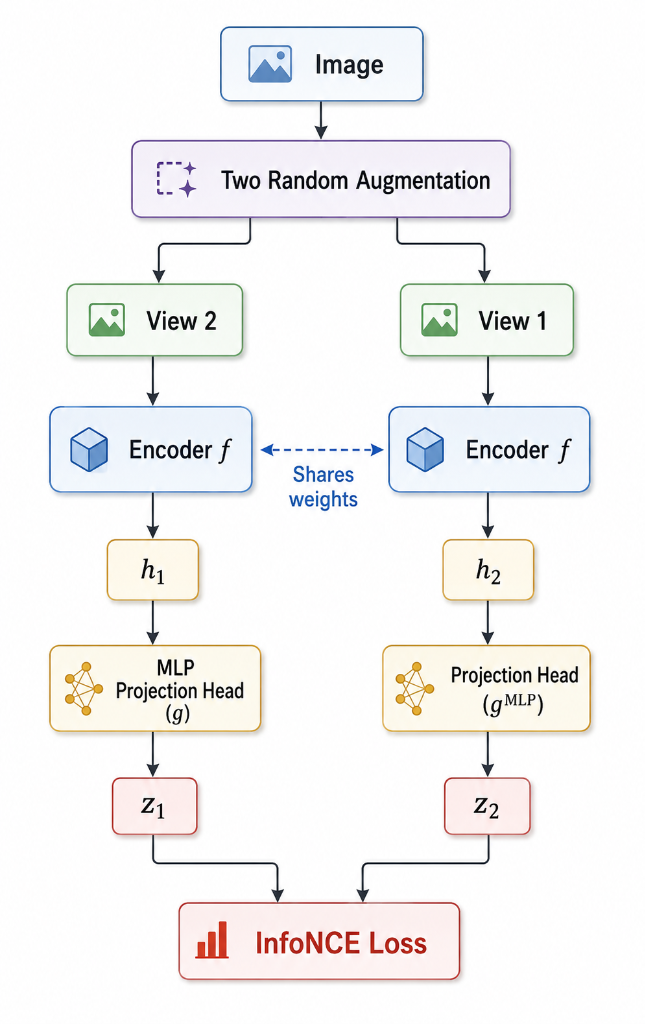
\includegraphics[width=0.75\textwidth]{figures/fig_7_simclr_architecture.png}
    \caption{SimCLR Architecture Overview.}
    \label{fig:simclr_architecture}
\end{figure}

The two encoder branches share the same parameters.

Each input image is transformed twice using random augmentations. Typical augmentations include: Random Crop, Random Resize, Horizontal Flip, Color Jitter, Gaussian Blur, Random Grayscale. The two resulting images form a positive pair.

The encoder extracts visual features from each augmented image. Originally, \textbf{SimCLR} used a standard CNN such as ResNet-50, although any backbone can be used. The encoder produces a feature representation $h = f(x)$ where:
\begin{itemize}
    \item $x = \text{augmented img}$
    \item $h = \text{learned feature representation}$
\end{itemize}

One of \textbf{SimCLR}'s most important contributions is the Projection Head. Instead of computing the contrastive loss directly on the encoder output, \textbf{SimCLR} introduces a small MLP $z = g(h)$. Researchers found that applying the contrastive loss directly on the encoder representation reduces downstream performance.

(The encoder learns useful visual representations by maximizing agreement between different augmented views of the same image).

The projection head separates:
\begin{itemize}
    \item Representation learning (encoder output $h$)
    \item Contrastive optimization (projected embedding $z$)
\end{itemize}

After training:
\begin{itemize}
    \item The projection head is discarded.
    \item Only the encoder is kept.
\end{itemize}

This improves transfer learning performance.

The projected embeddings $z_1, z_2$ are normalized and compared using cosine similarity. The InfoNCE loss then:
\[
L = -\log \left( \frac{\exp\left( \frac{\text{sim}(z_1, z_2)}{\tau} \right)}{\sum_k \exp\left( \frac{\text{sim}(z_1, z_k)}{\tau} \right)} \right)
\]
\begin{itemize}
    \item Maximizes similarity between positive pairs.
    \item Minimizes similarity with all negative pairs in the batch.
\end{itemize}

\subsection{Batch Training}

\textbf{SimCLR} does not use a memory bank (images stocked in memory that always play the role of negative pairs).

Instead, all other images in the mini-batch serve as negative samples.

For a batch of $N$ images:
\begin{itemize}
    \item Two augmentations are created.
    \item Total samples become $2N$.
    \item Each sample has one positive pair.
    \item The remaining $2N - 2$ samples are negatives.
\end{itemize}

As a result, larger batch sizes provide more negative samples and generally improve representation learning.

\subsection{Advantages}

\textbf{SimCLR} demonstrated that strong self-supervised representations can be learned using a simple framework.

Advantages include:
\begin{itemize}
    \item No labeled data required.
    \item Simple architecture.
    \item Strong downstream performance.
    \item Easy to implement.
    \item Foundation for many later S.S.L methods.
\end{itemize}

\subsection{Limitations}

\begin{itemize}
    \item Requires very large batch size.
    \item Large GPU memory consumption.
    \item Performance depends heavily on data augmentation.
    \item No memory bank for storing negatives.
\end{itemize}

These limitations motivated the development of \textbf{MoCo}.

\section{MoCo (Momentum Contrast)}

Although \textbf{SimCLR} demonstrated that contrastive learning could learn powerful visual representations, it had a major limitation: it required extremely large batch sizes. To provide enough negative samples, training \textbf{SimCLR} often required multiple GPUs and thousands of images per batch, making it impractical for many researchers.

To overcome this limitation, Facebook AI introduced Momentum Contrast (\textbf{MoCo}) in 2020. Instead of relying on large batches, \textbf{MoCo} maintains a dynamic dictionary of negative samples using a memory queue and a momentum encoder.

The key idea behind \textbf{MoCo} is simple: instead of generating negative samples only from the current mini-batch, maintain a large queue of embeddings computed from previous mini-batches. This allows the model to use thousands of negative samples while training with relatively small batch sizes.

\begin{figure}[H]
    \centering
    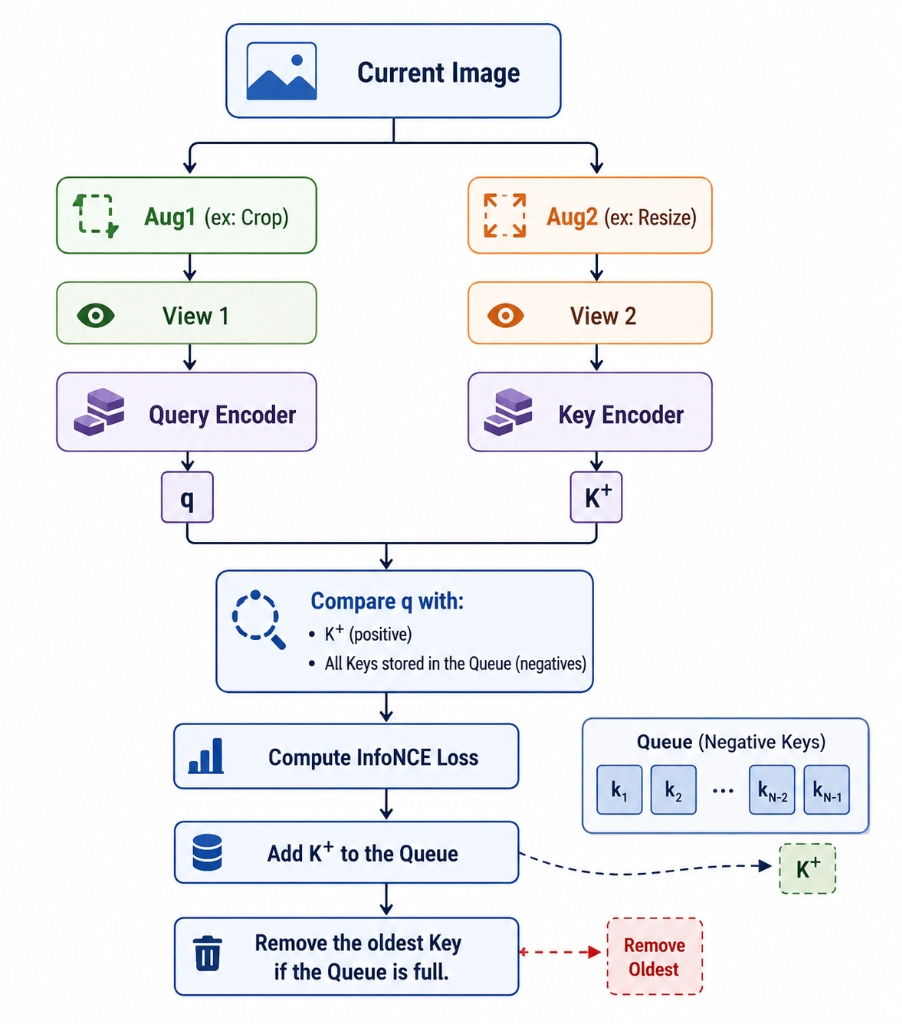
\includegraphics[width=0.82\textwidth]{figures/fig_7_moco_architecture.jpg}
    \caption{MoCo (Momentum Contrast) Architecture Overview.}
    \label{fig:moco_architecture}
\end{figure}

Unlike \textbf{SimCLR}, the two encoders do not share weights directly.

\subsection{MoCo Training Process}

\subsubsection{Step 1: Generate Two Views}
A training image is randomly augmented twice, producing two different views of the same image. These two views form a positive pair.
\[
\text{img} \longrightarrow \text{View 1}, \quad \text{View 2}
\]

\subsubsection{Step 2: Compute the Query Embedding}
The first view is passed through the Query Encoder, which is the main network being trained.

The query embedding is computed as:
\[
q = f_q(x)
\]
The Query Encoder parameters are updated normally using backpropagation after each training iteration.

\subsubsection{Step 3: Compute the Positive Key}
The second view is passed through the Momentum Encoder, which is not updated by gradient descent. Instead, its parameters are updated using an Exponential Moving Average (EMA) of the Query Encoder:
\[
\theta_K = m \theta_K + (1 - m) \theta_q
\]
where:
\begin{itemize}
    \item $\theta_q$ are the Query Encoder parameters.
    \item $\theta_K$ are the Momentum Encoder parameters.
    \item $m$ is the momentum coefficient (typically 0.999).
\end{itemize}

This slow update keeps the key representations stable during training.
\[
\text{View 2} \longrightarrow \text{Momentum Encoder} \longrightarrow \text{Positive Key } (K^+)
\]

\subsubsection{Step 4: Retrieve Negative Samples}
\textbf{MoCo} introduces a Memory Queue, which stores key embeddings generated during previous training iterations.
\[
\text{Memory Key}: [K_1], [K_2], [K_3], \dots, [K_n]
\]
Instead of using only the current mini-batch as in \textbf{SimCLR}, \textbf{MoCo} retrieves all the embeddings stored in this queue. These embeddings serve as the negative samples.

\subsubsection{Step 5: Compute the Contrastive Loss}
For each query embedding, the model compares:
\begin{itemize}
    \item The corresponding positive key $K^+$.
    \item All negative keys stored in the memory queue.
\end{itemize}

\[
\begin{array}{c|l c}
q & K^+ & (\text{Positive}) \quad \checkmark \\
  & K_1 & (\text{Negative}) \quad \times \\
  & K_2 & (\text{Negative}) \quad \times \\
  & K_3 & (\text{Negative}) \quad \times \\
  & \dots &
\end{array}
\]

The InfoNCE Loss encourages the query to become closer to its positive key while moving away from all negative keys.

\subsubsection{Step 6: Update the Models}
After computing the InfoNCE loss:
\begin{itemize}
    \item The Query Encoder is updated through backpropagation.
    \item The Momentum Encoder is updated using the EMA equation rather than gradients.
\end{itemize}

This ensures that the key embeddings evolve smoothly over time.

\subsubsection{Step 7: Update the Memory Queue}
Finally, the newly computed positive $K^+$ is inserted into the memory queue. If the queue is full, the oldest embedding is removed.
\[
\text{Queue Before}: [K_1], [K_2], [K_3], \dots, [K_n] \rightsquigarrow \text{Queue After}: [K_2], [K_3], [K_4], \dots, [K_n], [K^+]
\]

The queue therefore acts as a dynamic dictionary of negative samples, allowing \textbf{MoCo} to train with small mini-batches while benefiting from a large number of negatives.

\subsection{Why Use a Momentum Encoder?}

If the queue were generated by a rapidly changing encoder, key representations in the queue would become inconsistent across training iterations, causing loss computation instability. The Momentum Encoder evolves slowly through EMA updates, ensuring that embeddings in the queue remain relatively stable and improving the quality of the contrastive learning process.

\subsection{Advantages}

Compared with \textbf{SimCLR}:
\begin{itemize}
    \item Small mini-batches are sufficient.
    \item Large number of negative samples.
    \item Lower GPU memory requirements.
    \item More efficient training.
    \item High-quality representations.
\end{itemize}

\subsection{Limitations}

Despite its success, \textbf{MoCo} still relies on negative samples:
\begin{itemize}
    \item Selecting effective negatives.
    \item False negatives (different images representing similar semantics).
    \item Dependence on contrastive loss.
\end{itemize}

These limitations motivated researchers to explore negative-free learning, leading to methods such as \textbf{BYOL}.

\section{Why Contrastive Learning Isn't Enough?}

Contrastive Learning successfully learns visual representations by comparing positive and negative pairs, but it suffers from several limitations. It often requires large numbers of negative samples, leading to high computational costs. Additionally, some negatives are difficult to distinguish (hard negatives), while others are incorrectly treated as negatives despite sharing similar semantics (false negatives). Although negative samples prevent representation collapse, they also introduce complexity into the training process. These challenges motivated researchers to explore whether effective self-supervised learning could be achieved without any negative samples, leading to the development of \textbf{BYOL}.

\section{BYOL (Bootstrap Your Own Latent)}

Contrastive learning methods such as \textbf{SimCLR} and \textbf{MoCo} learn representations by comparing positive and negative pairs. Although effective, they require carefully selecting negative samples and suffer from problems such as false negatives and high computational cost.

In 2020, DeepMind introduced \textbf{BYOL}, showing that high-quality representations can be learned without using any negative samples. This result was surprising because it challenged the common belief that negative pairs were essential to prevent representation collapse.

\subsection{The Key Idea of BYOL}

Instead of pushing different images apart, \textbf{BYOL} learns by making two networks produce similar representations of two augmented views of the same image.

Unlike \textbf{SimCLR} or \textbf{MoCo}:
\begin{itemize}
    \item No Negative pairs
    \item No Memory Queue
    \item No Contrastive Loss
\end{itemize}

The model simply learns to predict its own representation.

\begin{figure}[H]
    \centering
    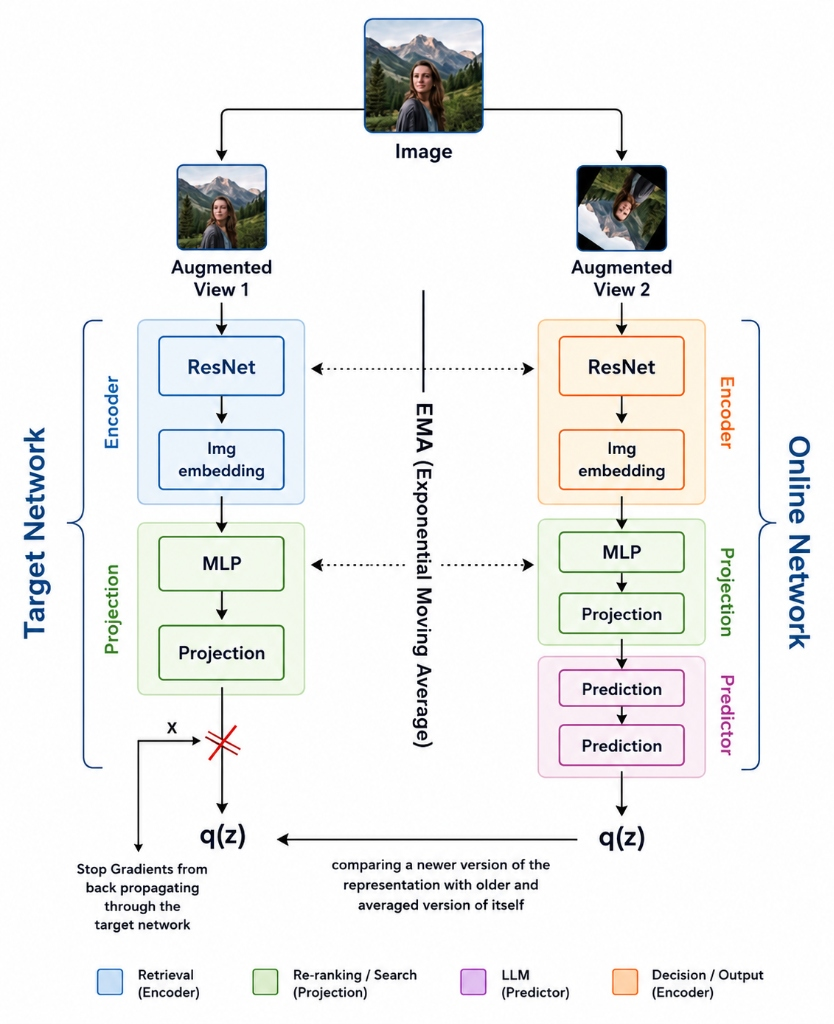
\includegraphics[width=0.82\textwidth]{figures/fig_7_byol_architecture.jpg}
    \caption{BYOL Architecture Overview: Target Network vs Online Network.}
    \label{fig:byol_architecture}
\end{figure}

\subsection{BYOL Architecture}

\textbf{BYOL} consists of two networks:
\begin{itemize}
    \item \textbf{Online Network}:
    \begin{itemize}
        \item Encoder
        \item Projection Head
        \item Prediction Head
    \end{itemize}
    \item \textbf{Target Network}:
    \begin{itemize}
        \item Encoder
        \item Projection Head
    \end{itemize}
\end{itemize}

Unlike the Online Network, the Target Network does not include a Prediction Head.

\subsubsection{I) Online Network}

The Online Network is the main network being trained. It receives one augmented view of the image and computes:
\[
h_o = f_o(x) \quad (f_o \text{ the encoder})
\]
The encoder output is passed through a Projection Head:
\[
z_o = g_o(h_o)
\]
and finally through a Prediction Head:
\[
q = p(z_o)
\]
The prediction vector $q$ is the output used for learning. Its parameters are updated normally using backpropagation.

\subsubsection{II) Target Network}

The Target Network processes the second augmented view. Unlike the Online Network, there is no Prediction Head. The Target Network is not updated using gradient descent. Instead, its parameters are updated using an Exponential Moving Average (EMA) of the Online Network:
\[
\theta_t = m \cdot \theta_t + (1 - m) \theta_o
\]
where:
\begin{itemize}
    \item $\theta_o$: Online Network parameters.
    \item $\theta_t$: Target Network parameters.
    \item $m$: momentum coefficient (typically $0.99 - 0.999$).
\end{itemize}

The EMA update allows the Target Network to evolve slowly, providing a stable learning target.

\subsection{Stop-Gradient Operation}

One of the key innovations of \textbf{BYOL} is the Stop-Gradient Operation. Before computing the loss, the output of the Target Network is detached from the computational graph. As a result:
\begin{itemize}
    \item The Target Network does not receive gradients.
    \item Only the Online Network is optimized through backpropagation.
\end{itemize}

This asymmetry is essential for stable learning.

\subsection{Loss Function}

The objective of \textbf{BYOL} is to make the prediction produced by the Online Network match the representation produced by the Target Network. Instead of the InfoNCE loss, \textbf{BYOL} minimizes the negative cosine similarity (\textbf{BYOL} does not use negative pairs at all; instead it only tries to make two representations of the same image as similar as possible):
\[
L = -\text{Cosine Similarity}(q, z)
\]
\[
L = -2 \frac{q^T z}{\|q\|_2 \cdot \|z\|_2}
\]

During training, the Online Network gradually learns to predict the Target Network representation.

\subsection{Detailed Training Step-by-Step}

For each training iteration (for every new image or mini-batch), \textbf{BYOL} processes two different augmented views of the same image. One view is passed through the online network, which produces the prediction vector $q$, while the other view is passed through the target network, which produces the target embedding $z$. Both vectors are $L_2$-normalized, so they have unit length, meaning that only their direction is compared rather than their magnitude. It then minimizes the negative cosine similarity $L = -\text{Cosine Similarity}(q, z)$, which encourages the prediction vector $q$ to become as aligned as possible with the target embedding $z$. During backpropagation, only the online network is updated, while the target network receives no gradients because of the stop-gradient operation. After the online network has been updated, the target network is not optimized by gradient descent; instead, its parameters are slowly updated using the EMA (Exponential Moving Average) of the online network's parameters. This entire procedure is repeated for every image or mini-batch throughout training, allowing the online network to progressively learn meaningful representations while the slowly evolving target network provides stable learning targets.

\subsection{Intuition: Why EMA Prevents Collapse}

\begin{itemize}
    \item If the reference model (target) changes as quickly as the online model, the optimization objective becomes highly unstable because the target is constantly shifting.
    \item By updating the target network only through EMA, \textbf{BYOL} provides a slowly evolving reference representation, allowing the online network to converge toward a stable objective.
\end{itemize}

\textbf{Imagine you're learning from a teacher:}
\begin{itemize}
    \item If the teacher rewrites the textbook after every lesson, the material you're trying to learn keeps changing, making it difficult to make consistent progress.
    \item If the teacher updates the textbook only occasionally, you have a stable reference to learn from before adapting to the new version.
\end{itemize}

This is exactly what the EMA target network does: it changes slowly, providing a stable learning target.

\begin{figure}[H]
    \centering
    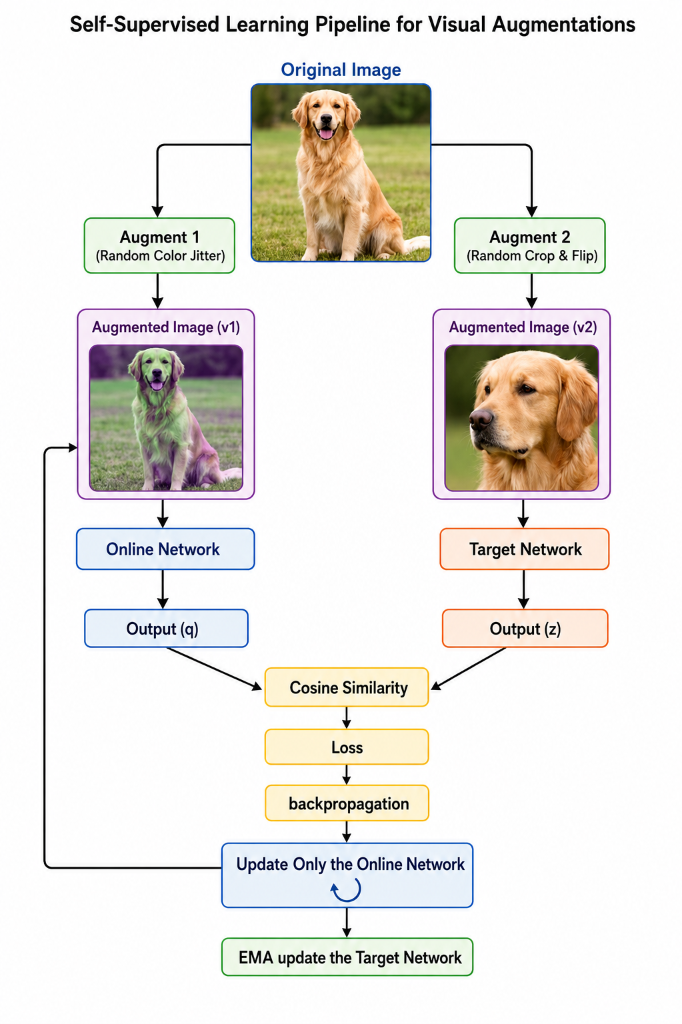
\includegraphics[width=0.82\textwidth]{figures/fig_7_byol_pipeline.png}
    \caption{Self-Supervised Learning Pipeline for Visual Augmentations in BYOL.}
    \label{fig:byol_pipeline}
\end{figure}

\subsection{Limitations of BYOL}

\begin{itemize}
    \item Requires two networks during training.
    \item Introduces EMA updates.
    \item Adds a Prediction Head, increasing architectural complexity.
    \item Initially lacked a complete theoretical explanation for why collapse does not occur.
\end{itemize}

\textbf{BYOL} successfully avoids representation collapse and achieves state-of-the-art performance, paving the way for later methods such as \textbf{SimSiam} and \textbf{DINO}.

\section{SimSiam (Simple Siamese Network)}

\textbf{BYOL} demonstrated that high-quality visual representations could be learned without negative samples. However, \textbf{BYOL} still required a Target Network updated via Exponential Moving Average (EMA), making the architecture more complex.

Researchers therefore asked an important question: \textbf{Is the momentum (EMA) Target Network really necessary?}

In 2021, Facebook AI introduced \textbf{SimSiam}, showing that self-supervised learning can still succeed without negative samples and without a momentum encoder. This was one of the most surprising discoveries in SSL.

By using a shared encoder, a Prediction Head, and a stop-gradient operation, it successfully learns meaningful visual representations without relying on negative samples or a memory queue. Its simplicity makes it one of the most elegant SSL methods and an important step toward later self-distillation approaches such as \textbf{DINO}.

\subsection{Main Idea of SimSiam}

The main idea of \textbf{SimSiam} is to learn by maximizing the similarity between augmented views of the same image.

Unlike \textbf{BYOL}:
\begin{itemize}
    \item No Momentum (EMA) Network
    \item No Memory Queue
    \item No Negative Samples
\end{itemize}

Instead, \textbf{SimSiam} relies on a shared Siamese network, a Prediction Head, and a Stop-Gradient operation to prevent collapse.

\subsection{Architecture}

\textbf{SimSiam} consists of two identical branches that share the same parameters.
Each branch contains:
\begin{itemize}
    \item Encoder
    \item Projection Head
\end{itemize}

For one direction of the loss, one branch passes through the Prediction Head and is compared with the stop-gradient output of the other branch. The full \textbf{SimSiam} algorithm then repeats this in the opposite direction.

\begin{figure}[H]
    \centering
    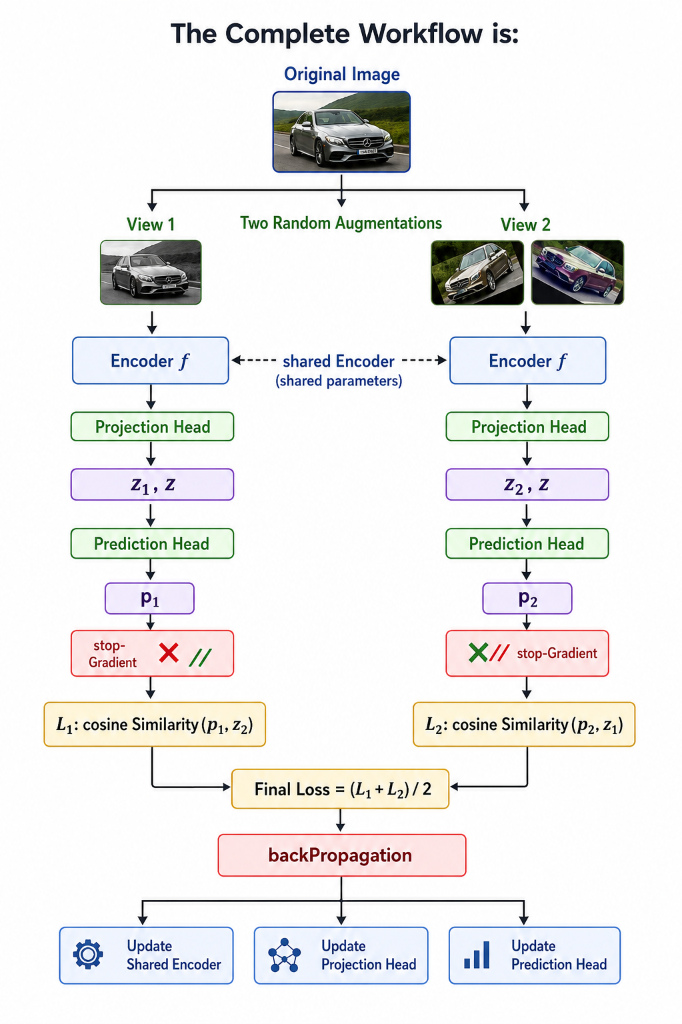
\includegraphics[width=0.82\textwidth]{figures/fig_7_simsiam_complete_workflow.png}
    \caption{The Complete Workflow of SimSiam.}
    \label{fig:simsiam_complete_workflow}
\end{figure}

\subsection{Splitting Architecture into 2 Branches}

Alternatively, we can split this architecture into two distinct loss branches:

\subsubsection{Loss $L_1$ Branch}
\begin{figure}[H]
    \centering
    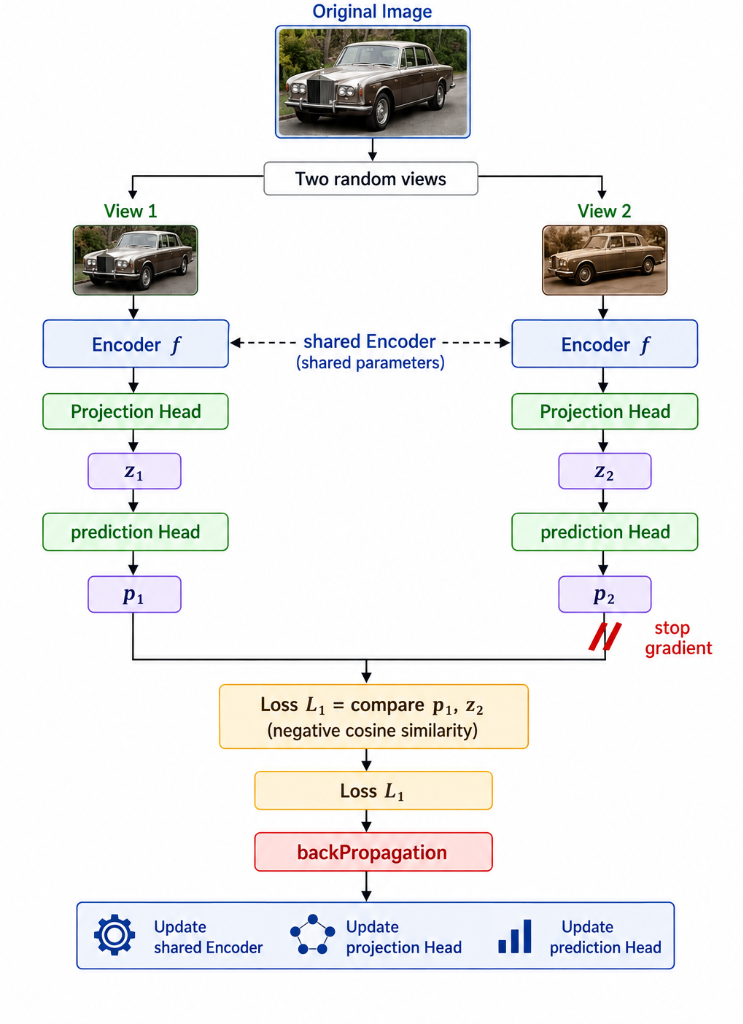
\includegraphics[width=0.78\textwidth]{figures/fig_7_simsiam_l1.png}
    \caption{SimSiam Loss $L_1$ Branch Architecture.}
    \label{fig:simsiam_l1}
\end{figure}

\subsubsection{Loss $L_2$ Branch}
\begin{figure}[H]
    \centering
    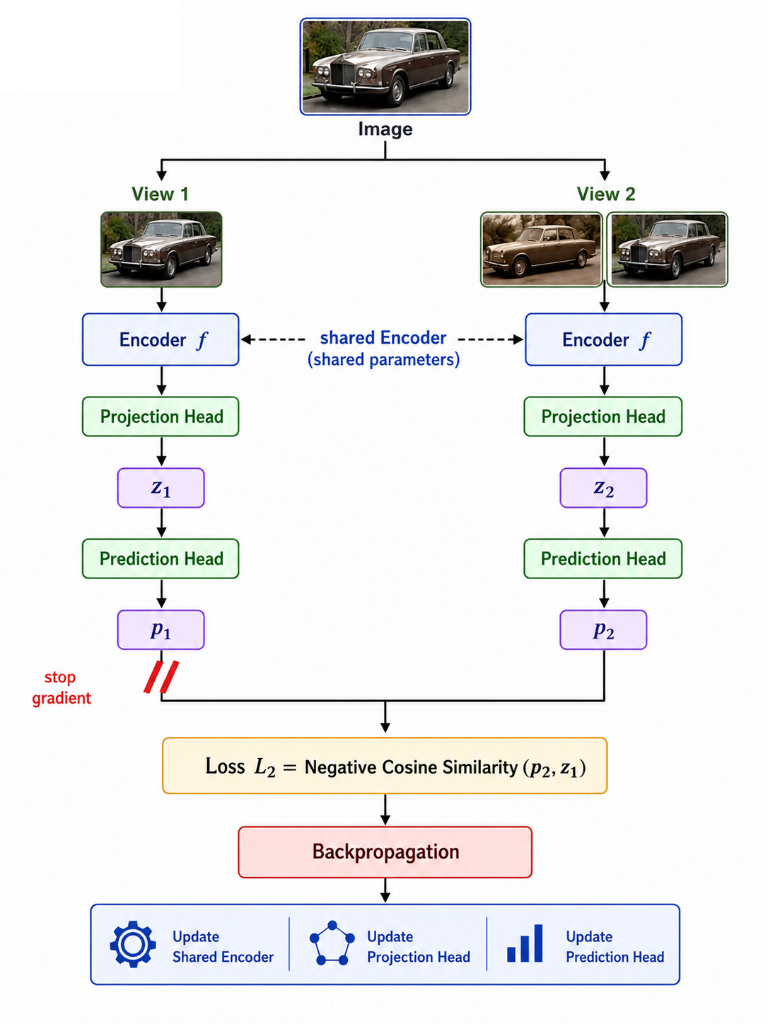
\includegraphics[width=0.78\textwidth]{figures/fig_7_simsiam_l2.png}
    \caption{SimSiam Loss $L_2$ Branch Architecture.}
    \label{fig:simsiam_l2}
\end{figure}

So \textbf{SimSiam} computes the loss symmetrically:
\begin{itemize}
    \item The first loss:
    \[
    L_1(p_1, z_2)
    \]
    \item Then the roles are swapped to compute the second loss:
    \[
    L_2(p_2, z_1)
    \]
\end{itemize}

Finally:
\[
L = \frac{L_1 + L_2}{2}
\]

\begin{itemize}
    \item $L_1$: compares prediction from branch 1 with the representation from branch 2 (after stop-gradient).
    \item $L_2$: compares prediction from branch 2 with the representation from branch 1 (after stop-gradient).
\end{itemize}

\subsection{Advantages of SimSiam}

\begin{itemize}
    \item Very Simple architecture.
    \item Only One encoder.
    \item No EMA update.
    \item No Memory Queue.
    \item No Negative Samples.
    \item Lower Computational Cost than \textbf{BYOL}.
    \item Competitive downstream performance.
\end{itemize}

\subsection{Limitations of SimSiam}

Despite its simplicity, \textbf{SimSiam} has some limitations:
\begin{itemize}
    \item More Sensitive to training settings than \textbf{BYOL}.
    \item Slightly lower performance than more recent methods such as \textbf{DINO}.
    \item Theoretical understanding of Collapse Prevention remains incomplete.
\end{itemize}

Although the precise theoretical explanation is still being studied, experiments show that removing the Stop Gradient causes the model to collapse.

\section{DINO (Distillation with No Labels)}

Although BYOL and SimSiam demonstrated that self-supervised learning could be performed without negative samples, researchers continued searching for methods capable of learning even richer visual representations.

In 2021, Facebook AI introduced \textbf{DINO} (\textbf{Di}stillation with \textbf{no} \textbf{L}abels). Instead of learning by directly matching representations, DINO adopts a teacher-student framework, where a student network learns to imitate a teacher network. Unlike traditional Knowledge Distillation, both networks are trained without labels, making the entire process self-supervised.

One of DINO's most remarkable discoveries is that the learned representations naturally capture object boundaries and semantic regions, allowing Vision Transformers to exhibit \textbf{emergent segmentation} without any segmentation labels.

Unlike BYOL, DINO predicts probability distributions rather than embeddings, and introduces Multi-Crop Training, Centering, and Sharpening to stabilize learning and avoid collapse. These innovations enable DINO to learn highly semantic visual representations and make it one of the most influential self-supervised learning methods for Vision Transformers.

\subsection{Main Idea of DINO}

The main idea of DINO is to train a student network to predict the output probability distribution produced by a teacher network for different augmented views of the same image.

Unlike BYOL:
\begin{itemize}
    \item The student predicts a probability distribution, not just an embedding.
    \item The teacher acts as a slowly evolving target.
    \item Additional mechanisms (Centering and Sharpening) stabilize training and prevent collapse.
\end{itemize}

DINO is therefore considered a \textbf{self-distillation} method.

\subsection{DINO Architecture}

DINO consists of two networks:
\begin{itemize}
    \item \textbf{Student Network}
    \item \textbf{Teacher Network}
\end{itemize}

Both networks contain:
\begin{enumerate}
    \item An Encoder (usually a Vision Transformer, ViT).
    \item A Projection Head.
\end{enumerate}

Unlike BYOL, neither network contains a separate prediction head. The teacher network is updated using an Exponential Moving Average (EMA) of the student network's parameters.
\clearpage
\begin{figure}[htbp]
    \centering
    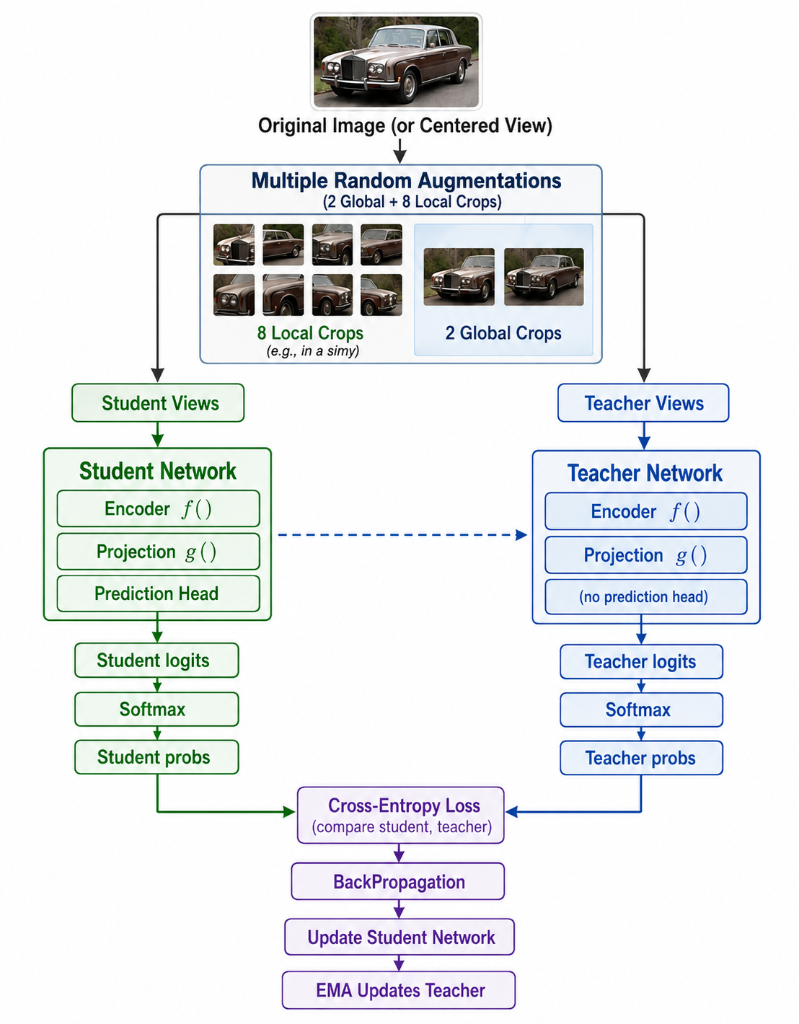
\includegraphics[width=0.85\linewidth]{figures/fig_7_dino_architecture.png}
    \caption{DINO Self-Distillation Architecture with Student and Teacher Networks.}
    \label{fig:dino_architecture}
\end{figure}

\subsection{Multi-Crop Training}

Before DINO, models learned that two global views correspond to the same object (e.g., entire cat $\rightarrow$ head, ear, or tail). A good representation should recognize that all these crops belong to the same object. Neither SimCLR nor BYOL explicitly enforced local-to-global view matching. This motivated DINO to introduce \textbf{Multi-Crop Training}.

Instead of generating only two views, DINO generates many views of an image:

\begin{figure}[htbp]
    \centering
    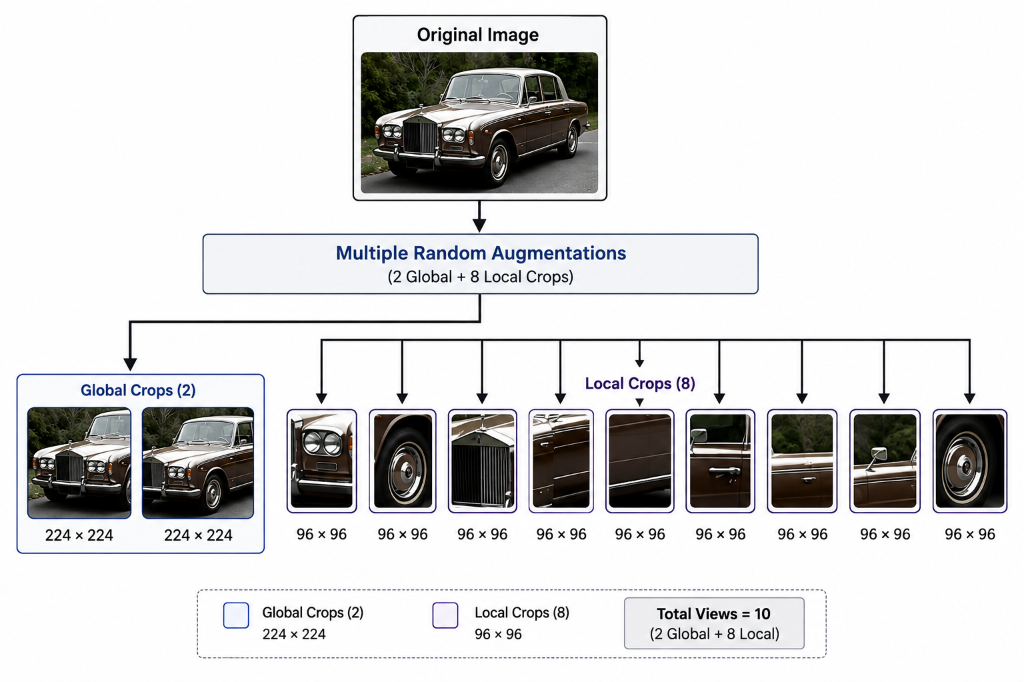
\includegraphics[width=0.9\linewidth]{figures/fig_7_dino_multicrop.png}
    \caption{DINO Multi-Crop Strategy with 2 Global Crops ($224 \times 224$) and 8 Local Crops ($96 \times 96$).}
    \label{fig:dino_multicrop}
\end{figure}

Typically, DINO creates:
\begin{itemize}
    \item \textbf{2 Global Crops}: Large crops ($224 \times 224$) covering most of the image, capturing global semantics.
    \item \textbf{8 Local Crops}: Small crops ($96 \times 96$) covering smaller regions (e.g., dog head, leg, or tail).
\end{itemize}

The student receives all crops (both global and local), while the teacher receives only global crops. The student must learn that local crops and global crops represent the same object, greatly improving representation robustness.

\subsection{Preventing Collapse: Centering and Sharpening}

While multi-crop training increases feature richness, another problem appears: the teacher network can start producing identical uniform outputs for every image, leading to representation collapse. To solve this, DINO introduces \textbf{Centering} and \textbf{Sharpening}.

\subsubsection{Centering}

Without centering, after many iterations, the teacher might output identical uniform distributions for all inputs (e.g., assigning 25\% probability to every class: Cat 25\%, Dog 25\%, Car 25\%, Bird 25\%). Every image receives the same prediction, causing the student to copy this trivial solution.

\textbf{The Solution (Centering):} DINO maintains a running average (center $c$) of the teacher's outputs across iterations. The center is subtracted from the teacher's logits before applying softmax:
\[
y_t = \text{Softmax}\left( \frac{g_t - c}{T_t} \right)
\]
where $g_t$ are the teacher logits, $c$ is the running center, and $T_t$ is the teacher temperature. Centering prevents any single dimension from dominating, encouraging the teacher to utilize the entire representation space.

\subsubsection{Sharpening}

While centering prevents collapse to a constant vector, it can cause the teacher's probability distribution to become overly soft (e.g., Cat 25\%, Dog 23\%, Car 22\%, Bird 20\%), leaving the student with an uninformative target.

\textbf{The Solution (Sharpening):} DINO applies a small temperature parameter $T_t < 1$ in the teacher's Softmax (e.g., $T_t = 0.04$ vs. $T=1.0$). Dividing by a small temperature scales up the largest logit, sharpening the distribution (e.g., turning probabilities like $[0.4, 0.26, 0.03, 0.01]$ into a decisive $[0.9999, 0.0001, 0, 0]$).

Combining Centering and Sharpening balances the predictions and keeps the teacher confident, producing a strong learning signal for the student.

\subsection{Loss Function}

The student predicts a probability distribution $P_s$, and the teacher produces a probability distribution $P_t$. The objective is to minimize the Cross-Entropy loss between them:
\[
\mathcal{L} = - \sum P_t \log P_s
\]
Unlike SimCLR or BYOL:
\begin{itemize}
    \item No Cosine Similarity.
    \item No InfoNCE loss.
    \item No Negative Samples.
\end{itemize}
The student simply learns to imitate the teacher's distribution.

\subsection{Emergent Segmentation}

One of DINO's most remarkable properties is that Vision Transformers (ViTs) trained with DINO naturally learn attention maps that align with object boundaries without any segmentation labels. The attention maps highlight:
\begin{itemize}
    \item Main objects.
    \item Semantic regions.
    \item Object contours.
\end{itemize}
This phenomenon is known as \textbf{emergent segmentation} and remains one of DINO's key milestones.

\subsection{Advantages and Limitations of DINO}

\textbf{Advantages:}
\begin{itemize}
    \item No labels required.
    \item No negative samples needed.
    \item Superior representations for Vision Transformers.
    \item Multi-scale learning via multi-crop training.
    \item Emergent segmentation capabilities.
    \item Strong performance on downstream transfer tasks.
\end{itemize}

\textbf{Limitations:}
\begin{itemize}
    \item More complex than BYOL and SimSiam.
    \item Requires delicate hyperparameter tuning for Centering and Sharpening.
    \item Higher computational cost due to multi-crop training (10 views per image).
\end{itemize}

\section{DINOv2}

The original DINO demonstrated that self-distillation could learn excellent visual representations without labels. However, it was trained on relatively small datasets compared to modern foundation models.

In 2023, Meta introduced \textbf{DINOv2} to answer a fundamental question: \emph{Can DINO become a general-purpose vision foundation model, similar to how GPT became a foundation model for language?}

Rather than proposing a completely new learning algorithm, DINOv2 focuses on scaling up the DINO framework using carefully curated data, larger ViT architectures, and optimized training techniques.

\subsection{Automatic Dataset Curation}

A core innovation of DINOv2 is its automatic data curation pipeline. Instead of uncurated web scraping, Meta built an automated pipeline to clean and balance a massive image repository by removing:
\begin{itemize}
    \item Duplicate images.
    \item Low-quality or corrupted images.
    \item Watermarked images.
    \item Near-identical copies and noisy samples.
\end{itemize}
This resulted in a clean, diverse dataset (LVD-142M), proving that data quality is as important as model architecture.

\subsection{Large-Scale Training and Downstream Tasks}

DINOv2 was trained on hundreds of millions of curated images. The resulting representations transfer seamlessly across diverse computer vision tasks without task-specific fine-tuning:
\begin{itemize}
    \item Image Classification \& Retrieval
    \item Object Detection \& Instance Segmentation
    \item Depth Estimation \& Semantic Segmentation
    \item Few-shot and Zero-shot Learning
\end{itemize}

\section{Masked Image Modeling (MIM)}

Until now, all self-supervised methods studied (SimCLR, MoCo, BYOL, SimSiam, DINO) belong to the view-comparison family: learning by contrasting or matching two augmented views of an image.

Researchers proposed a fundamentally different approach: \emph{Can a model learn visual representations by reconstructing missing parts of an image instead of comparing two full images?} This idea gave birth to \textbf{Masked Image Modeling (MIM)}.

\begin{figure}[htbp]
    \centering
    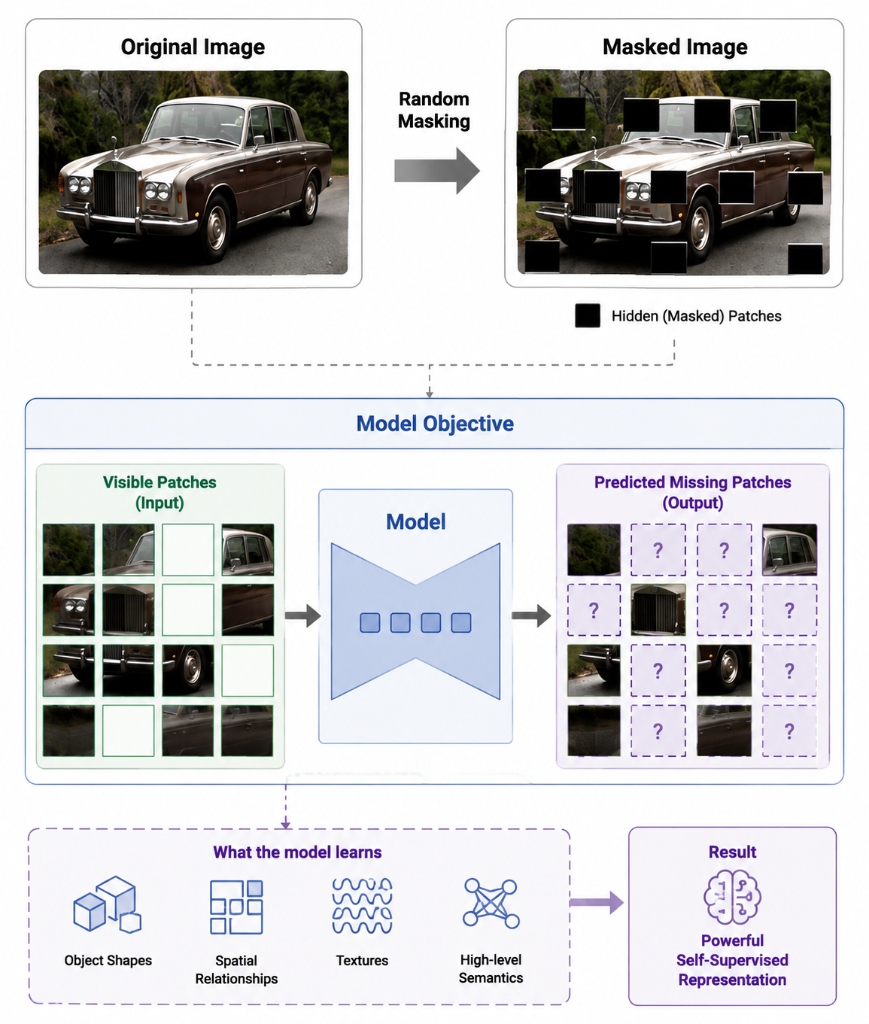
\includegraphics[width=0.85\linewidth]{figures/fig_7_mim_objective.jpg}
    \caption{Masked Image Modeling (MIM) Objective: predicting hidden patches from visible context.}
    \label{fig:mim_objective}
\end{figure}

\subsection{Main Idea of MIM}

Instead of feeding a complete image, MIM intentionally hides (masks) a large percentage of image patches (e.g., 40\%--75\%). The model receives only the visible patches and must infer the missing regions.

To predict the hidden patches accurately, the model must understand:
\begin{itemize}
    \item Object shapes and boundaries.
    \item Spatial relationships.
    \item Textures and high-level semantics.
\end{itemize}

Since the original unmasked image already contains the ground-truth content, supervision comes directly from the image itself—making MIM a pure self-supervised task.

\subsection{Target Prediction Types in MIM}

Different MIM architectures target different representation formats:
\begin{itemize}
    \item \textbf{BEiT}: Predicts discrete \textbf{visual tokens}.
    \item \textbf{MAE}: Reconstructs raw \textbf{pixel values}.
    \item \textbf{iBOT}: Combines patch reconstruction with self-distillation.
\end{itemize}

\section{BEiT (BERT Pre-Training of Image Transformers)}

Introduced by Microsoft, \textbf{BEiT} adapts BERT's masked language modeling concept to computer vision. Often referred to as \emph{"BERT for Images"}, BEiT masks image patches and trains a Vision Transformer to predict discrete visual tokens generated by a pretrained, frozen visual tokenizer (dVAE).

\subsection{From BERT to BEiT}

In NLP, BERT masks words in a sentence and predicts them:
\[
\text{The cat is [MASK] on the sofa} \longrightarrow \text{predict: sleeping}
\]
BEiT operates identically for images: it masks a subset of image patches and predicts the corresponding visual token for each masked patch.

\subsection{Visual Tokens}

A visual token is analogous to a word ID in NLP vocabulary. For example, in BERT, $\text{cat} \rightarrow \text{Token ID 384}$. In BEiT, an image patch (e.g., a dog's ear) is mapped by a Discrete VAE (dVAE) tokenizer into a discrete token ID (e.g., $\text{Token 812}$).

Instead of predicting millions of raw RGB values, BEiT predicts discrete token IDs that represent high-level visual concepts.

\subsection{BEiT Architecture}

BEiT consists of two separate components:
\begin{enumerate}
    \item \textbf{Visual Tokenizer (Frozen)}: Pretrained dVAE that converts image patches into discrete visual tokens. Its weights are fixed during BEiT training.
    \item \textbf{Vision Transformer (Trainable)}: Processes masked patch embeddings and predicts the missing visual token IDs.
\end{enumerate}
\clearpage
\begin{figure}[htbp]
    \centering
    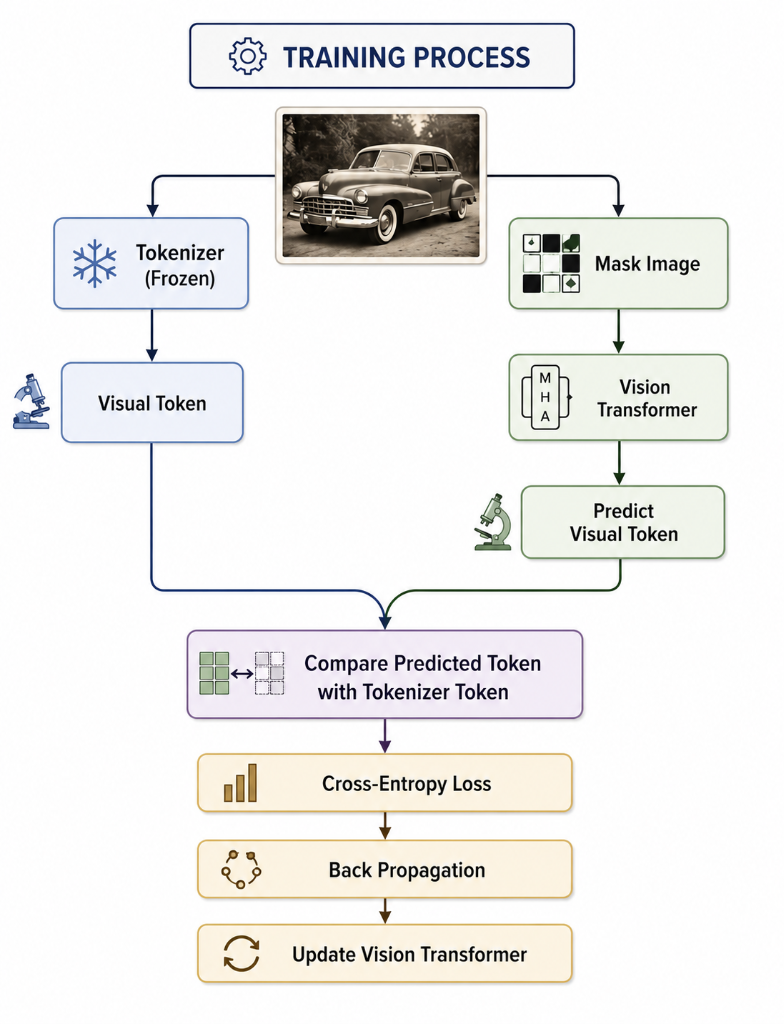
\includegraphics[width=0.85\linewidth]{figures/fig_7_beit_training_process.png}
    \caption{BEiT Training Process with Frozen Tokenizer and Trainable Vision Transformer.}
    \label{fig:beit_training_process}
\end{figure}

\subsection{Loss Function}

Since the target is a discrete token ID, BEiT uses standard \textbf{Cross-Entropy Loss} between the predicted token probability distribution and the ground-truth token ID produced by the frozen tokenizer.

\subsection{Why Predict Tokens Instead of Pixels?}

Predicting raw pixel values is highly ambiguous: a masked sky patch could have many valid RGB color shades. In contrast, predicting a visual token forces the model to focus on abstract semantic categories rather than low-level pixel noise.

\subsection{Advantages and Limitations of BEiT}

\textbf{Advantages:}
\begin{itemize}
    \item Learns high-level semantic representations.
    \item Directly leverages BERT's proven masked modeling paradigm.
    \item Avoids pixel reconstruction ambiguity.
    \item Delivers strong transfer performance on vision tasks.
\end{itemize}

\textbf{Limitations:}
\begin{itemize}
    \item Requires a separate pretrained visual tokenizer (dVAE).
    \item Two-stage training pipeline (stage 1: train tokenizer; stage 2: train BEiT).
    \item Performance is bounded by tokenizer quality.
    \item Additional computational complexity from the tokenizer.
\end{itemize}

\subsection{MAE (Masked Autoencoders)}

Although BEiT achieved excellent performance, it introduced a new fundamental question: \emph{why do we need a separate visual tokenizer?} Training the tokenizer requires an additional model, extra computation, and a two-stage training pipeline.

Researchers at Meta (He et al., 2021) asked a simpler question: \textbf{Can we remove the tokenizer completely and directly reconstruct missing image patches?}

The answer was \textbf{MAE (Masked Autoencoders)}. MAE demonstrated that simply reconstructing missing raw pixels is sufficient to learn powerful visual representations—provided the architecture is designed asymmetrically and efficiently.

\subsubsection{Key Simplification}

MAE simplifies Masked Image Modeling by eliminating the pretrained visual tokenizer. Instead, it:
\begin{enumerate}
    \item Masks a very high proportion of image patches (approximately \textbf{75\%}).
    \item Trains a Vision Transformer encoder on only the remaining \textbf{25\% visible patches}.
    \item Uses a lightweight decoder to reconstruct the original pixel values of the missing patches.
    \item Minimizes reconstruction error using \textbf{Mean Squared Error (MSE)}.
\end{enumerate}

Unlike BEiT, MAE uses:
\begin{itemize}
    \item No visual tokenizer.
    \item No visual token vocabulary.
    \item Direct pixel-level reconstruction.
\end{itemize}

\subsubsection{Why a 75\% Masking Ratio?}

One of MAE's most surprising insights is its extremely high masking ratio. While NLP models like BERT mask 15\% of words and early vision methods masked $\sim$40\%, MAE masks \textbf{75\% of all image patches}, leaving only 25\% visible.


This high masking ratio is necessary because images contain immense spatial redundancy. For example, in an image of a dog, even if most of the image is covered, a human can easily infer the missing parts from surrounding context. A low masking ratio (e.g., 15\%) makes the reconstruction task trivial, allowing the model to extrapolate pixels locally without learning deep semantic structure. Masking 75\% forces the model to understand global scene composition.

\subsubsection{Asymmetric Encoder-Decoder Architecture}

MAE introduces a novel asymmetric design where the heavy encoder only sees visible patches:

\begin{itemize}
    \item \textbf{Encoder}: A standard Vision Transformer that processes \emph{only} unmasked visible patches (25\%). Masked patches are completely discarded before the encoder. This reduces computational cost dramatically (roughly a $4\times$ reduction in FLOPs).
    \item \textbf{Decoder}: A lightweight Transformer that receives the latent representations of visible patches plus shared learnable \textbf{Mask Tokens} (`[MASK]`) for missing positions. It reconstructs full-resolution RGB pixels. The decoder is discarded after pretraining.
\end{itemize}
\clearpage
\begin{figure}[htbp]
    \centering
    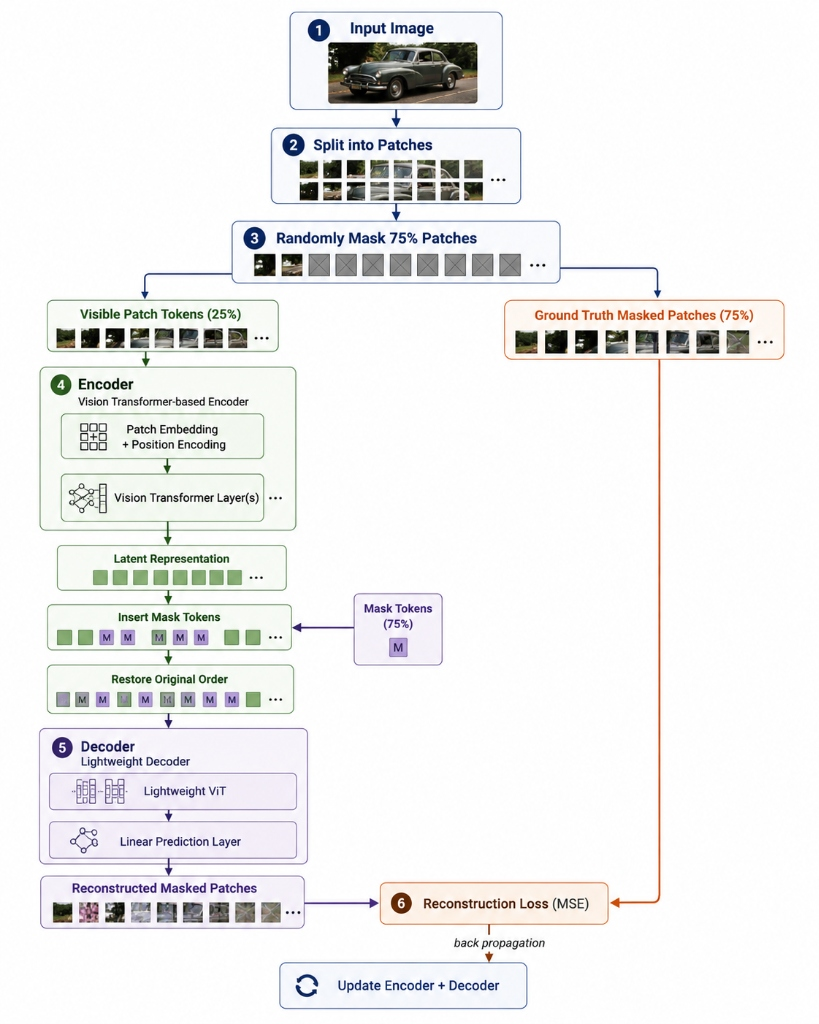
\includegraphics[width=0.85\linewidth]{figures/fig_7_mae_architecture.png}
    \caption{MAE Architecture: Processing only 25\% visible patches through the encoder, inserting mask tokens, and reconstructing raw pixels with a lightweight decoder.}
    \label{fig:mae_architecture}
\end{figure}

\subsubsection{Reconstruction Loss}

The reconstruction loss is the Mean Squared Error (MSE) between predicted pixel values $\hat{x}_i$ and original RGB pixels $x_i$, computed exclusively over masked patches $M$:
\[
\mathcal{L}_{\text{MSE}} = \frac{1}{|M|} \sum_{i \in M} \|x_i - \hat{x}_i\|^2
\]

\subsubsection{Fine-Tuning}

After pretraining, the lightweight decoder is removed. The pretrained ViT encoder is retained and fine-tuned for downstream computer vision tasks such as:
\begin{itemize}
    \item Image Classification.
    \item Object Detection.
    \item Semantic Segmentation.
\end{itemize}

\subsubsection{Advantages of MAE}
\begin{itemize}
    \item \textbf{No Visual Tokenizer}: Eliminates dVAE pretraining and complex tokenizers.
    \item \textbf{High Efficiency}: Asymmetric design allows processing only $25\%$ of patches in the encoder.
    \item \textbf{Strong Semantics}: High masking ratio forces global conceptual reasoning.
    \item \textbf{Scalability}: Scales exceptionally well to massive ViT models (ViT-Huge, ViT-Giant).
\end{itemize}

\subsection{iBOT (Image BERT with Online Tokenizer)}

By late 2021, self-supervised learning for vision had divided into two distinct paradigms:
\begin{enumerate}
    \item \textbf{Distillation-based Methods} (BYOL, SimSiam, DINO): Excel at learning \textbf{global image representations} by enforcing consistency between augmented views.
    \item \textbf{Masked Image Modeling} (BEiT, MAE): Excel at learning \textbf{local patch representations} by reconstructing missing regions.
\end{enumerate}

Researchers at ByteDance (Zhou et al., 2021) asked: \emph{Can we combine the strengths of both paradigms?} This led to \textbf{iBOT (Image BERT with Online Tokenizer)}, which unifies self-distillation and masked image modeling in a single framework.

\begin{figure}[htbp]
    \centering
    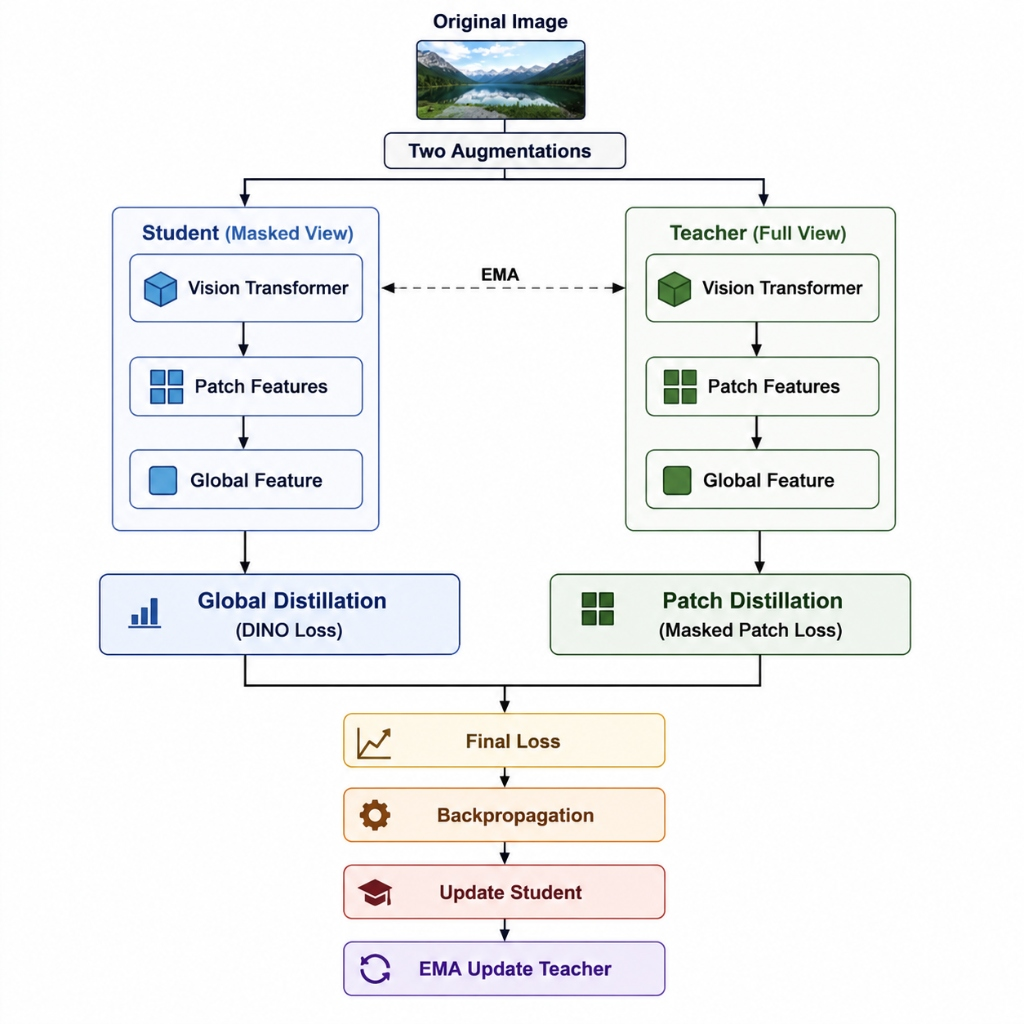
\includegraphics[width=0.85\linewidth]{figures/fig_7_ibot_overview.png}
    \caption{iBOT High-Level Overview: Combining Global Distillation (DINO Loss) and Patch Distillation (Masked Patch Loss).}
    \label{fig:ibot_overview}
\end{figure}

\subsubsection{Main Idea}

Instead of choosing between global consistency and local reconstruction, iBOT performs both simultaneously:
\begin{itemize}
    \item \textbf{Global Task}: Learns a global representation for the entire image (like DINO).
    \item \textbf{Patch Task}: Learns detailed semantic representations for individual masked patches (like BEiT/MAE).
\end{itemize}

For example, when given an image of a dog:
\begin{itemize}
    \item DINO learns: \emph{"This entire scene is a dog"} (Global).
    \item MAE learns: \emph{"This hidden patch should be RGB $(125, 117, 110)$"} (Local pixel).
    \item \textbf{iBOT learns both}: \emph{"This image is a dog"} AND \emph{"This hidden patch represents a dog's ear"} (Semantic patch representation).
\end{itemize}

\begin{figure}[htbp]
    \centering
    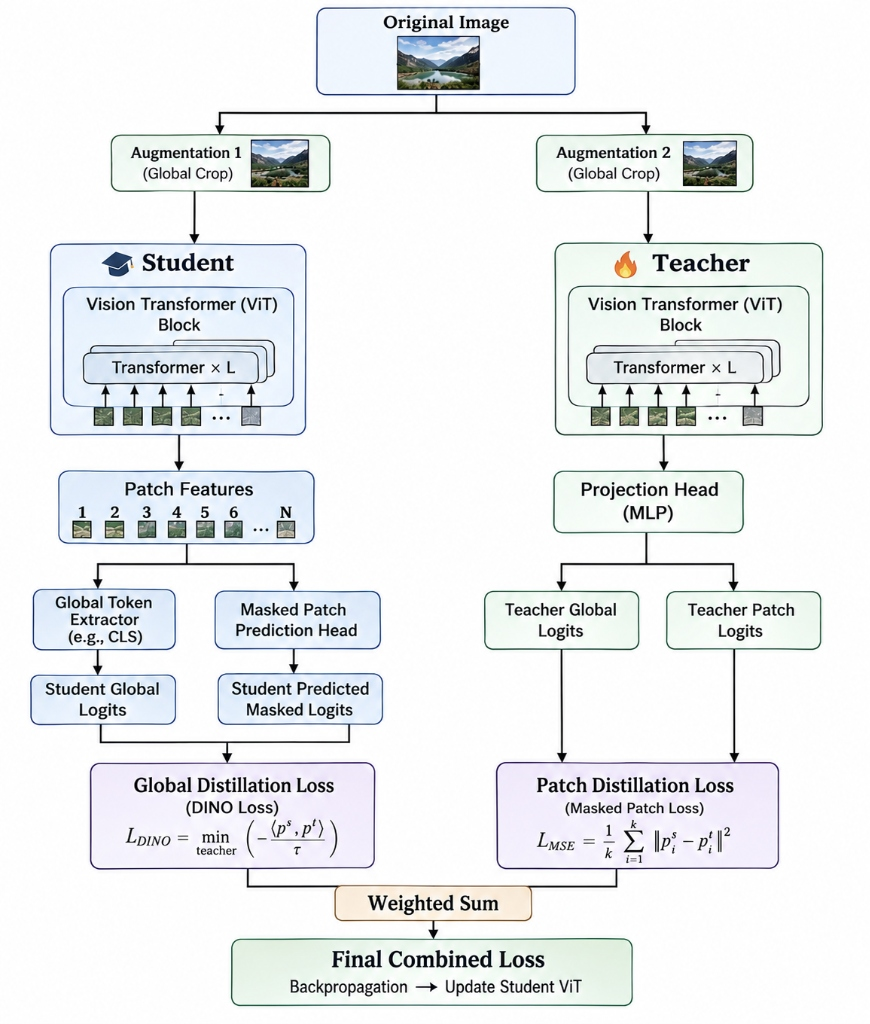
\includegraphics[width=0.9\linewidth]{figures/fig_7_ibot_detailed.jpg}
    \caption{Detailed iBOT Teacher-Student Learning Framework.}
    \label{fig:ibot_detailed}
\end{figure}

\subsubsection{iBOT Architecture \& Targets}

iBOT employs a DINO-like Student-Teacher setup:
\begin{itemize}
    \item \textbf{Teacher Network}: Processes the unmasked full image and generates semantic targets for both the global image and individual patches. Updated via Exponential Moving Average (EMA).
    \item \textbf{Student Network}: Processes masked views of the image and learns to predict both global logits and teacher patch features simultaneously.
\end{itemize}

Crucially, \textbf{iBOT does not reconstruct raw pixels (unlike MAE) nor predict discrete token IDs (unlike BEiT)}. Instead, the student predicts the \textbf{teacher's high-level patch feature representations}.

\subsubsection{iBOT Loss Function}

iBOT optimizes a dual objective:
\[
\mathcal{L}_{\text{iBOT}} = \mathcal{L}_{\text{global}} + \mathcal{L}_{\text{patch}}
\]
\begin{itemize}
    \item $\mathcal{L}_{\text{global}}$: Cross-entropy loss matching student global representation to teacher global representation (DINO loss).
    \item $\mathcal{L}_{\text{patch}}$: Cross-entropy loss matching student masked patch predictions to corresponding teacher patch representations.
\end{itemize}

\subsubsection{Advantages and Limitations}
\textbf{Advantages:}
\begin{itemize}
    \item Unifies global image semantics and fine-grained local patch understanding.
    \item Self-conditioned online tokenizer eliminates the need for an offline dVAE.
    \item Outperforms previous SSL methods on dense prediction tasks (segmentation, detection).
\end{itemize}

\textbf{Limitations:}
\begin{itemize}
    \item Higher computational complexity (requires Teacher, Student, EMA, and dual losses).
    \item More memory-intensive training pipeline.
\end{itemize}


\section{Modern Self-Supervised Learning Frontiers}

Self-supervised learning continues to evolve rapidly. This section highlights four cutting-edge frameworks that shaped modern representation learning.

\subsection{Barlow Twins (Learning by Reducing Redundancy)}

Proposed by Zbontar et al. (2021), \textbf{Barlow Twins} addresses a central question: \emph{Can we learn effective representations without negative pairs, teacher networks, queues, or pixel reconstruction?}

\begin{figure}[htbp]
    \centering
    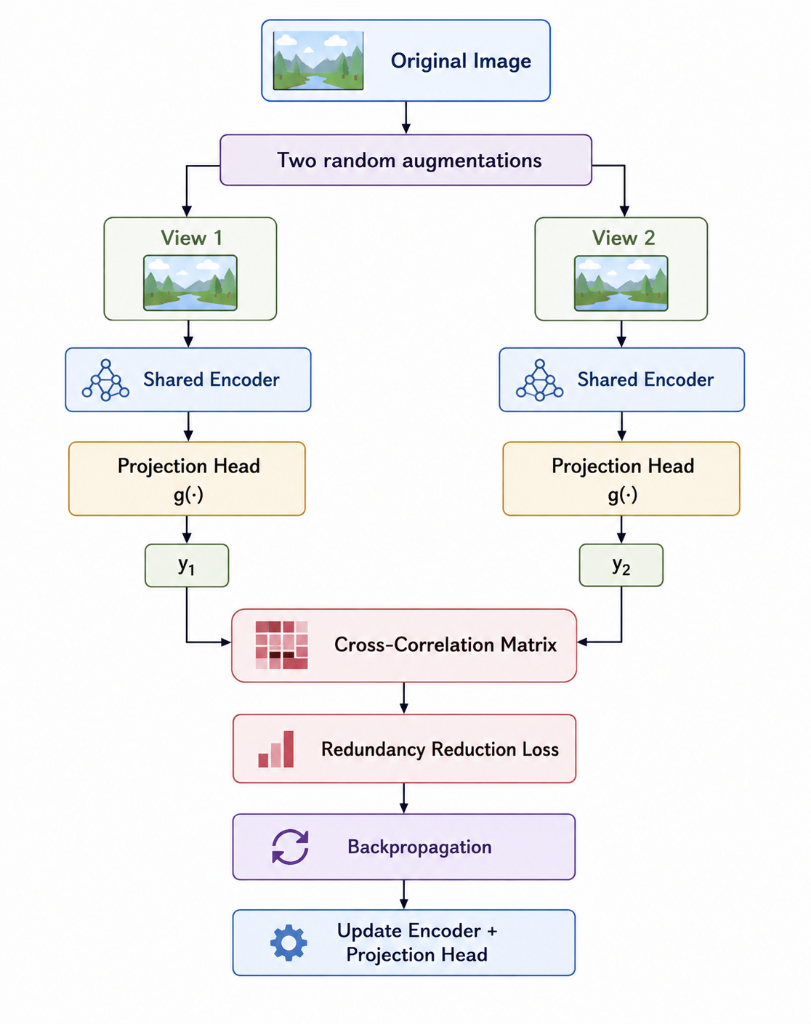
\includegraphics[width=0.85\linewidth]{figures/fig_7_barlow_twins.png}
    \caption{Barlow Twins Architecture: Computing the Cross-Correlation Matrix between twin representations to enforce Redundancy Reduction.}
    \label{fig:barlow_twins}
\end{figure}

Barlow Twins applies neuroscience-inspired \textbf{redundancy reduction} to representation learning.

\subsubsection{Core Principle}

Given two augmented views $y_1, y_2$ of the same image processed through a shared encoder and projection head, Barlow Twins computes their normalized \textbf{Cross-Correlation Matrix} $\mathcal{C}$:
\[
\mathcal{C}_{ij} = \frac{\sum_b z_{b,i}^{(1)} z_{b,j}^{(2)}}{\sqrt{\sum_b (z_{b,i}^{(1)})^2} \sqrt{\sum_b (z_{b,j}^{(2)})^2}}
\]
where $b$ indexes batch samples, and $i, j$ index vector feature dimensions.

The objective forces $\mathcal{C}$ to resemble the Identity matrix $I$:
\begin{itemize}
    \item \textbf{Diagonal Elements ($\mathcal{C}_{ii} \to 1$)}: \emph{Invariance term}—forces the same feature component to be invariant to data augmentations.
    \item \textbf{Off-Diagonal Elements ($\mathcal{C}_{ij} \to 0, i \neq j$)}: \emph{Redundancy Reduction term}—decorrelates different feature components, ensuring each vector entry captures unique, independent information.
\end{itemize}

The loss function is defined as:
\[
\mathcal{L}_{\text{BT}} = \sum_i (1 - \mathcal{C}_{ii})^2 + \lambda \sum_i \sum_{j \neq i} \mathcal{C}_{ij}^2
\]
\vspace{5cm}

\subsection{VICReg (Variance, InVariance, Covariance)}

Proposed by Bardes et al. (2021), \textbf{VICReg} expands on non-contrastive learning by explicitly decomposing representation regularization into three explicit terms.
\clearpage
\begin{figure}[htbp]
    \centering
    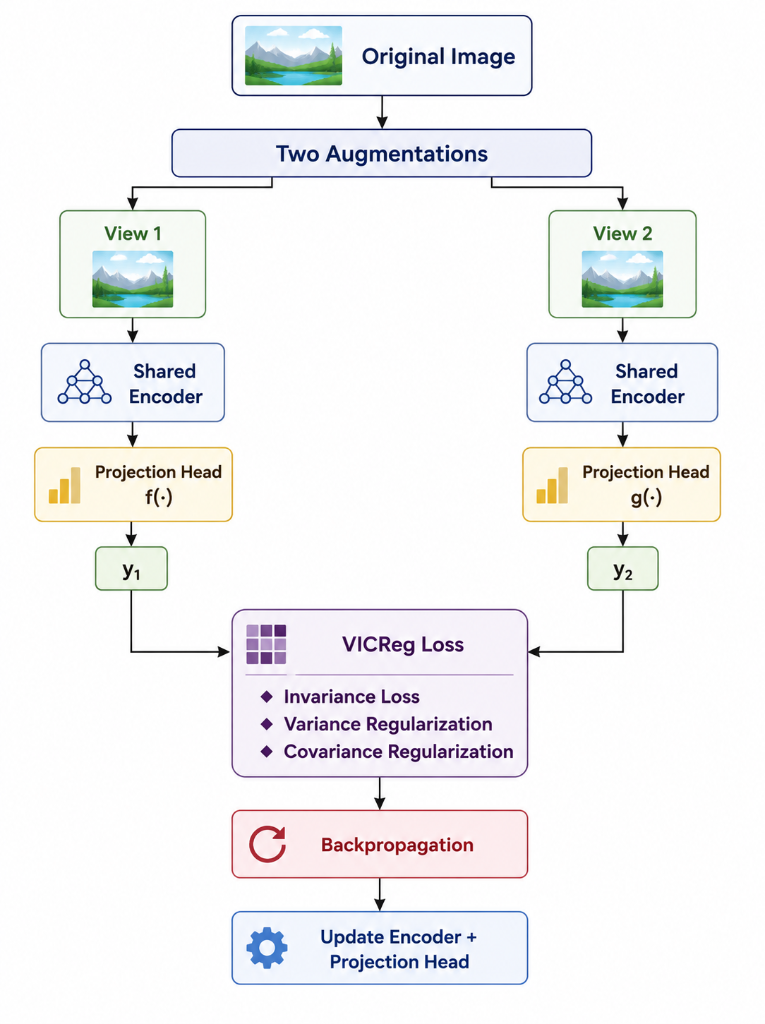
\includegraphics[width=0.85\linewidth]{figures/fig_7_vicreg_architecture.png}
    \caption{VICReg Architecture: Explicitly optimizing Invariance Loss, Variance Regularization, and Covariance Regularization.}
    \label{fig:vicreg}
\end{figure}

\clearpage
\vspace{5cm}
VICReg avoids representation collapse without negative pairs or asymmetric teacher architectures by enforcing three criteria directly on representations $Z_1, Z_2$:
\begin{enumerate}
    \item \textbf{Invariance ($s$)}: Standard mean squared error between representations of augmented views.
    \item \textbf{Variance ($v$)}: Hinge loss forcing the standard deviation of each feature dimension across a batch to remain above a threshold $\gamma > 0$ (prevents feature collapse to a constant).
    \item \textbf{Covariance ($c$)}: Off-diagonal covariance matrix penalty, decorrelating different features to eliminate redundancy.
\end{enumerate}

\[
\mathcal{L}_{\text{VICReg}} = \lambda s(Z_1, Z_2) + \mu [v(Z_1) + v(Z_2)] + \nu [c(Z_1) + c(Z_2)]
\]

VICReg is widely valued for its mathematical simplicity, stability, and absence of asymmetric architectural tricks.
\vspace{5cm}

\subsection{I-JEPA (Image Joint-Embedding Predictive Architecture)}

Proposed by Yann LeCun and Meta AI (Assran et al., 2023), \textbf{I-JEPA} (Image Joint-Embedding Predictive Architecture) addresses a fundamental limitation of pixel-reconstruction models such as MAE: \emph{Predicting every pixel forces the model to allocate capacity to unpredictable, low-level details (e.g., exact textures or noise), which are often irrelevant for learning high-level semantic representations.}

\clearpage
\begin{figure}[htbp]
    \centering
    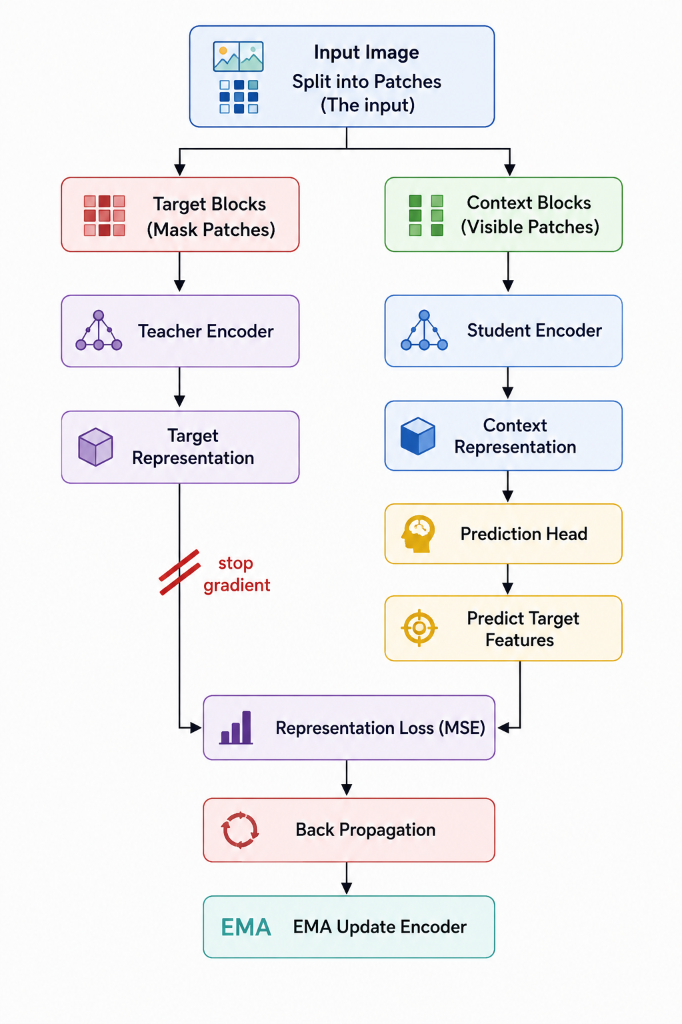
\includegraphics[width=0.85\linewidth]{figures/fig_7_ijepa_architecture.png}
    \caption{I-JEPA architecture: predicting target representations from visible context representations in the embedding space.}
    \label{fig:ijepa}
\end{figure}
\clearpage

\subsubsection{Main Idea}

Instead of reconstructing pixels in the image space, \textbf{I-JEPA predicts high-level semantic representations directly in the embedding space}.

\begin{itemize}
    \item \textbf{Context Blocks} (visible image patches) are processed by a \textbf{Student Encoder} to produce context embeddings.
    
    \item \textbf{Target Blocks} (masked image regions) are processed by a \textbf{Teacher Encoder} (with stop-gradient) to produce target embeddings.
    
    \item A \textbf{Predictor} receives the context embeddings together with the positional embeddings of the target blocks and predicts the corresponding target embeddings.
    
    \item \textbf{Training Objective:} Minimize the Mean Squared Error (MSE) between the predicted target embeddings and the target embeddings produced by the Teacher Encoder.
\end{itemize}

By predicting semantic representations rather than reconstructing pixels, \textbf{I-JEPA} learns meaningful high-level features while avoiding unnecessary focus on unpredictable low-level image details. This enables the model to learn more robust and semantically rich visual representations for downstream tasks.


\vspace{5cm}
\subsection{CLIP (Contrastive Language-Image Pre-training)}

Introduced by OpenAI (Radford et al., 2021), \textbf{CLIP} bridges computer vision and natural language processing using multimodal contrastive learning.
\clearpage
\begin{figure}[htbp]
    \centering
    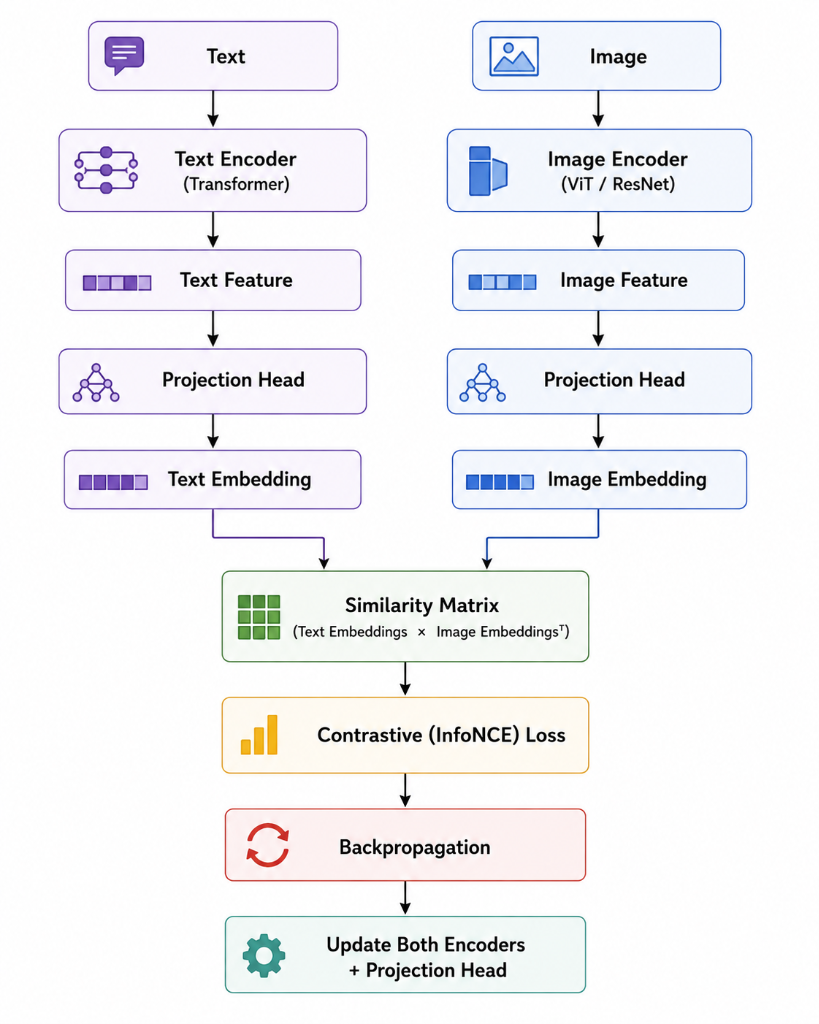
\includegraphics[width=0.85\linewidth]{figures/fig_7_clip_architecture.png}
    \caption{CLIP Multimodal Contrastive Learning Architecture.}
    \label{fig:clip}
\end{figure}
\clearpage

\vspace{5cm}
\subsubsection{Main Idea}

CLIP jointly trains an \textbf{Image Encoder} (ViT or ResNet) and a \textbf{Text Encoder} (Transformer) on 400 million (image, text) pairs curated from the internet.

Given a batch of $N$ (image, text) pairs:
\begin{enumerate}
    \item Images are encoded into image embeddings $I_1, I_2, \dots, I_N$.
    \item Text prompts are encoded into text embeddings $T_1, T_2, \dots, T_N$.
    \item An $N \times N$ similarity matrix is computed via cosine similarity: $S_{i,j} = \text{sim}(I_i, T_j)$.
    \item Symmetric InfoNCE loss maximizes similarity along the diagonal ($I_i, T_i$) while minimizing off-diagonal pairs ($I_i, T_j, i \neq j$).
\end{enumerate}

\subsubsection{Zero-Shot Classification}

The key breakthrough of CLIP is \textbf{Zero-Shot Transfer}. After pretraining, CLIP can perform image classification without any task-specific fine-tuning:
\begin{enumerate}
    \item Text prompts are created for each target class (e.g., \emph{"a photo of a [dog]"}, \emph{"a photo of a [cat]"}).
    \item Prompt text embeddings are generated using the Text Encoder.
    \item The test image embedding is matched against all text prompt embeddings via cosine similarity.
    \item The class corresponding to the highest similarity score is selected as the prediction.
\end{enumerate}

CLIP's robust zero-shot capabilities established it as the foundation for modern multimodal systems, including Stable Diffusion, DALL-E 2, and vision-LLMs.

\chapter{Autoencoders}

Traditional supervised learning requires labeled data. Autoencoders were created to answer a fundamental question: \emph{Can a neural network learn useful features from unlabeled data?} This is called \textbf{representation learning}.

A \textbf{representation} (embedding / latent vector) is a compact vector that captures the important information in the input. 
\[
\text{Example: Image } (150,528 \text{ pixels}) \longrightarrow \text{Embedding } (128 \text{ numbers})
\]

The goal is not just compression, but \textbf{preserving meaningful information}. Once a good embedding is learned, it can be reused for many downstream tasks: Classification, Object Detection, Segmentation, and more. This core idea is heavily utilized in modern foundation models such as BERT, GPT, and CLIP. Autoencoders were among the first neural networks designed specifically for learning embeddings.

\section*{Why Not PCA?}
Principal Component Analysis (PCA) also reduces dimensionality, but it has important limitations:
\begin{itemize}
    \item Works only with \textbf{linear relationships}.
    \item Cannot learn hierarchical features ($\text{edge} \rightarrow \text{eyes} \rightarrow \text{faces}$).
    \item Has a fixed linear transformation after training.
\end{itemize}
Autoencoders use deep neural networks, allowing them to learn complex non-linear representations.

\section{Vanilla Autoencoders}

\subsection{The Big Idea}
Autoencoders were introduced to solve the problem of learning useful representations without labels. Instead of predicting classes, they learn by reconstructing their own inputs. An encoder compresses the input into a low-dimensional latent representation, and a decoder reconstructs the original data from that representation. The bottleneck prevents the network from simply copying the input, forcing it to retain only the most informative features.

This simple reconstruction principle laid the foundation for many modern models including VAE, VQ-VAE, MAE, and the latent encoders used in Stable Diffusion.

Researchers proposed an elegant principle: instead of training a network with explicit supervision (\emph{``classify this image''}), instruct it to \emph{``compress this image, then reconstruct it''}. If the reconstruction is accurate, the compressed vector must preserve essential semantic information. In other words, the network learns representations without human labels.

\[
\text{Original Image} \longrightarrow \text{Encoder} \longrightarrow \text{Latent Vector} \longrightarrow \text{Decoder} \longrightarrow \text{Reconstructed Image}
\]

The training objective is:
\[
\text{Reconstructed Image} \approx \text{Original Image}
\]
No human labels are required because the image supervises itself. This makes autoencoders one of the earliest and purest forms of \textbf{self-supervised learning}.

\subsection{The Bottleneck}
The latent vector is intentionally constrained to be much smaller than the input:
\[
\text{Input } (150,528 \text{ values}) \longrightarrow \text{Bottleneck } (128 \text{ values}) \longrightarrow \text{Output } (150,528 \text{ values})
\]
This \textbf{bottleneck} forces the model to retain only the most critical information instead of trivially memorizing every pixel.

\subsection{Architecture of a Vanilla Autoencoder}


A vanilla autoencoder consists of two main component networks:
\begin{enumerate}
    \item \textbf{Encoder}: Compresses the high-dimensional input into a low-dimensional latent vector.
    \[
    150,528 \longrightarrow 4096 \longrightarrow 1024 \longrightarrow 256 \longrightarrow 64
    \]
    The final 64-dimensional output is called the \emph{Latent Vector}, \emph{Latent Representation}, or \emph{Embedding}.
    
    \item \textbf{Bottleneck}: Is the narrowest layer of the network where the latent vector is stored. Because information capacity is strictly limited, the network discards fine noise and retains fundamental structural features.
    
    \item \textbf{Decoder}: Reconstructs the original input from the latent vector.
    \[
    64 \longrightarrow 256 \longrightarrow 1024 \longrightarrow 4096 \longrightarrow 150,528
    \]
\end{enumerate}
\clearpage
\begin{figure}[htbp]
    \centering
    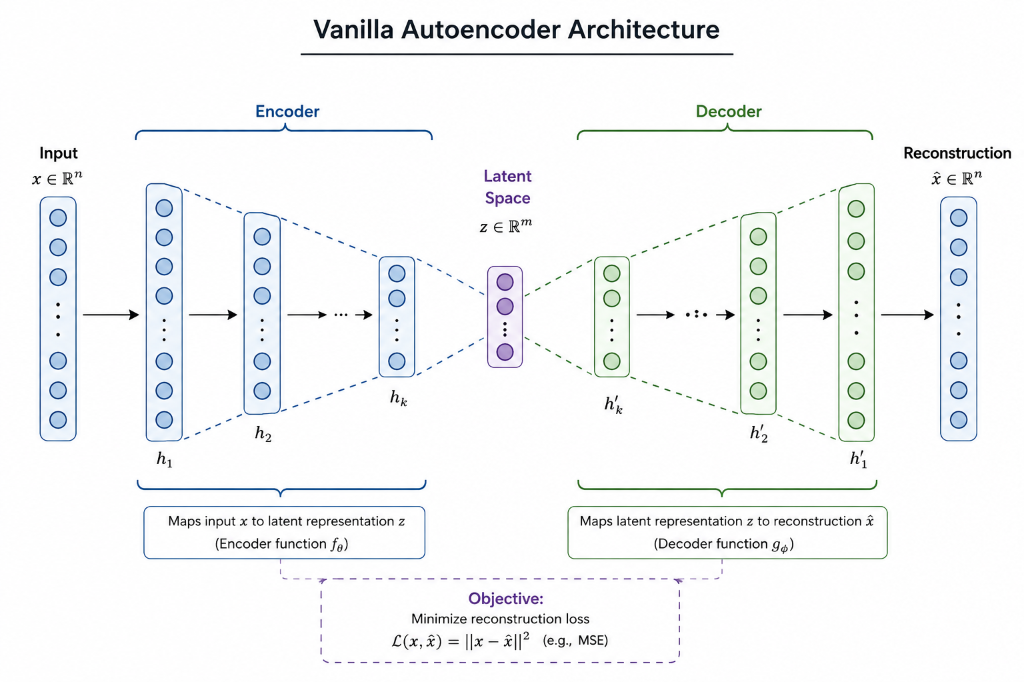
\includegraphics[width=0.85\linewidth]{figures/fig_8_vanilla_autoencoder_architecture.png}
    \caption{Vanilla Autoencoder Architecture showing Encoder, Latent Space, and Decoder.}
    \label{fig:vanilla_autoencoder_architecture}
\end{figure} 

\subsection{Training \& Reconstruction Loss}



During training, the reconstructed image $\hat{x}$ is compared with the original input $x$ using a \textbf{Reconstruction Loss}. For images, the most common loss function is Mean Squared Error (MSE):
\[
\mathcal{L}_{\text{recon}} = \| x - \hat{x} \|^2
\]
Backpropagation updates parameters across both the encoder and decoder simultaneously. Because the bottleneck restricts throughput, the encoder is forced to learn meaningful representations rather than simple copying.
\clearpage
\begin{figure}[htbp]
    \centering
    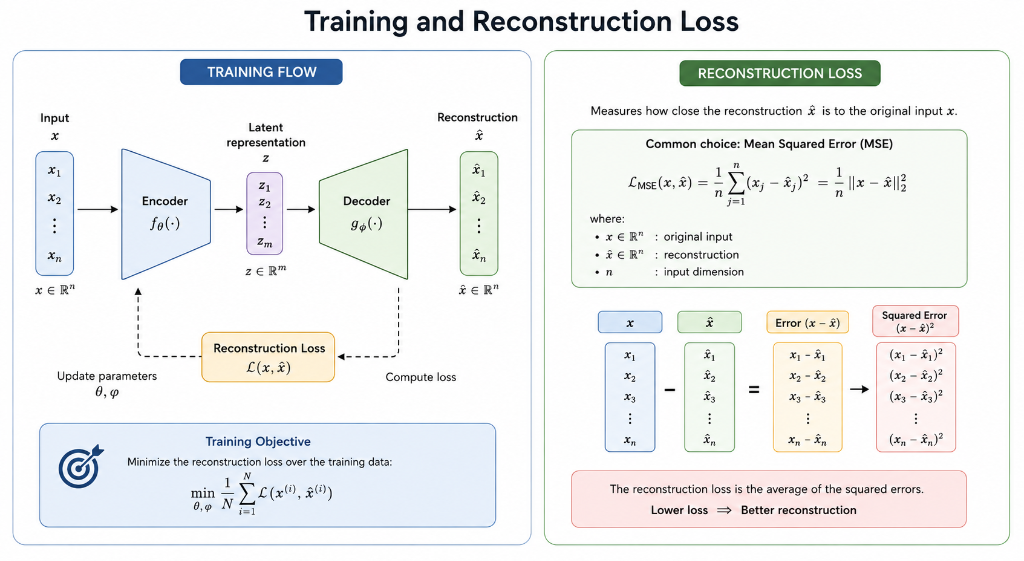
\includegraphics[width=0.95\linewidth]{figures/fig_8_training_and_reconstruction_loss.png}
    \caption{Training Flow and Reconstruction Loss formulation, showing Mean Squared Error (MSE) calculation across pixel dimensions and gradient update loops.}
    \label{fig:training_and_reconstruction_loss}
\end{figure}

\subsection*{Summary}
A vanilla autoencoder is composed of an encoder, a latent representation (bottleneck), and a decoder. The encoder compresses the input into a compact embedding, while the decoder reconstructs the original input from that embedding. During training, the reconstructed image is compared with the original using a reconstruction loss, and backpropagation updates both networks. Because the bottleneck severely limits the amount of information that can pass through, the encoder is forced to learn meaningful representations instead of simply copying the input.

\section{Latent Space Properties}

A \textbf{latent space} is the mathematical space containing all latent vectors (embeddings) produced by the encoder:
\begin{itemize}
    \item 2-dimensional latent vector $\longrightarrow$ 2D latent space
    \item 64-dimensional latent vector $\longrightarrow$ 64D latent space
\end{itemize}

Every input image becomes a point in this space where \textbf{similar inputs lie close together}. Without explicit labels, the encoder naturally clusters similar images because they require similar feature representations for accurate reconstruction. The latent space organizes data by \textbf{semantic similarity}, not raw pixel values. This property is crucial for:
\begin{itemize}
    \item Image Retrieval
    \item Clustering
    \item Similarity Search
\end{itemize}

\begin{figure}[htbp]
    \centering
    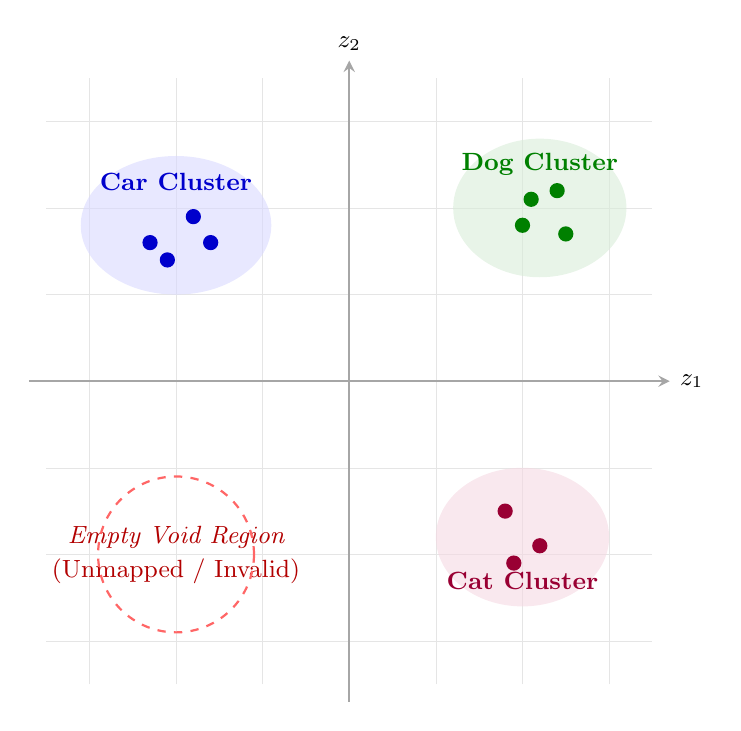
\begin{tikzpicture}[scale=1.1, >=stealth]
        % Background grid & axes
        \draw[very thin, color=gray!20] (-3.5,-3.5) grid (3.5,3.5);
        \draw[->, thick, color=gray!70] (-3.7,0) -- (3.7,0) node[right, black] {\small $z_1$};
        \draw[->, thick, color=gray!70] (0,-3.7) -- (0,3.7) node[above, black] {\small $z_2$};

        % Car Cluster (Top Left)
        \fill[blue!15, opacity=0.6] (-2,1.8) ellipse (1.1cm and 0.8cm);
        \node[blue!80!black, font=\bfseries\small] at (-2,2.3) {Car Cluster};
        \fill[blue!80!black] (-2.3,1.6) circle (2.5pt);
        \fill[blue!80!black] (-1.8,1.9) circle (2.5pt);
        \fill[blue!80!black] (-2.1,1.4) circle (2.5pt);
        \fill[blue!80!black] (-1.6,1.6) circle (2.5pt);

        % Dog Cluster (Top Right)
        \fill[green!50!black!15, opacity=0.6] (2.2,2.0) ellipse (1.0cm and 0.8cm);
        \node[green!50!black, font=\bfseries\small] at (2.2,2.5) {Dog Cluster};
        \fill[green!50!black] (2.0,1.8) circle (2.5pt);
        \fill[green!50!black] (2.4,2.2) circle (2.5pt);
        \fill[green!50!black] (2.1,2.1) circle (2.5pt);
        \fill[green!50!black] (2.5,1.7) circle (2.5pt);

        % Cat Cluster (Bottom Right)
        \fill[purple!15, opacity=0.6] (2.0,-1.8) ellipse (1.0cm and 0.8cm);
        \node[purple!80!black, font=\bfseries\small] at (2.0,-2.3) {Cat Cluster};
        \fill[purple!80!black] (1.8,-1.5) circle (2.5pt);
        \fill[purple!80!black] (2.2,-1.9) circle (2.5pt);
        \fill[purple!80!black] (1.9,-2.1) circle (2.5pt);

        % Empty Void Region (Bottom Left)
        \node[red!70!black, font=\itshape\small] at (-2.0,-1.8) {Empty Void Region};
        \node[red!70!black, font=\small] at (-2.0,-2.2) {(Unmapped / Invalid)};
        \draw[red!60, dashed, thick] (-2.0,-2.0) circle (0.9cm);
    \end{tikzpicture}
    \caption{Visualization of a 2D Latent Space learned by an Autoencoder. Similar semantic concepts (Cars, Dogs, Cats) naturally form clustered regions, while unpopulated areas represent empty void regions.}
    \label{fig:latent_space_visualization}
\end{figure}

\subsection{Latent Interpolation}
Suppose we take two latent vectors corresponding to a \textbf{DOG} at $(2, 3)$ and a \textbf{WOLF} at $(8, 5)$. What happens if we step gradually between them in the latent space?
\begin{align*}
(2, 3.0) &\longrightarrow \text{DOG} \\
(3, 3.5) &\longrightarrow \text{Dog-like} \\
(4, 4.0) &\longrightarrow \text{Half Dog, Half Wolf} \\
(5, 4.5) &\longrightarrow \text{Wolf-like} \\
(8, 5.0) &\longrightarrow \text{WOLF}
\end{align*}
Moving smoothly between latent vectors generates smooth transitions upon decoding. The decoder synthesizes intermediate images that were never in the original dataset. This operation is called \textbf{latent interpolation}.

\subsection{Limitation of Vanilla Autoencoders}
Because a vanilla autoencoder only maps training inputs to deterministic points, large portions of the latent space remain completely unmapped (empty regions).
\clearpage
\begin{figure}[htbp]
    \centering
    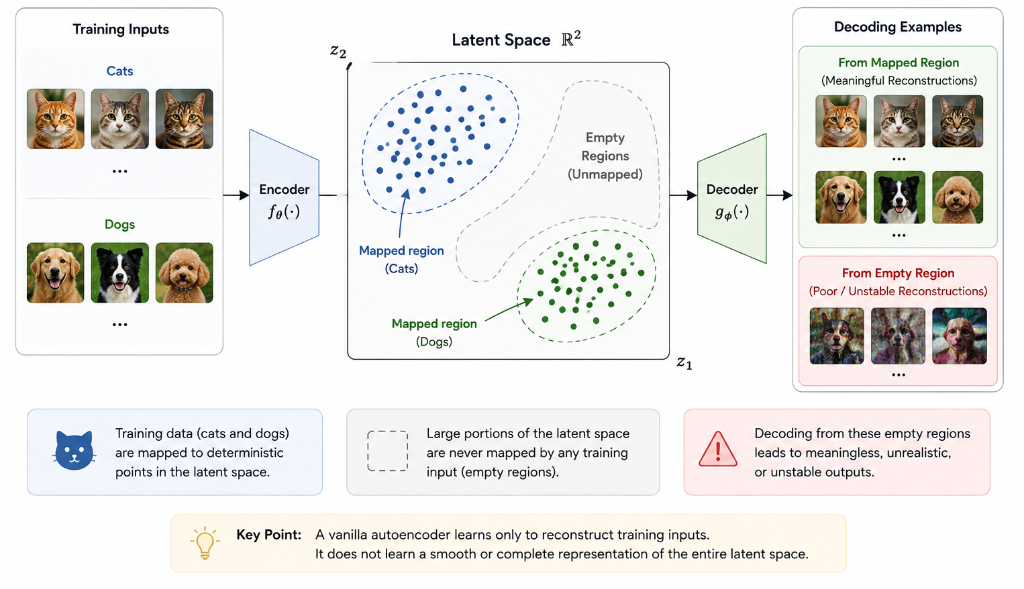
\includegraphics[width=0.95\linewidth]{figures/fig_8_latent_space_empty_regions.png}
    \caption{Deterministic latent space mapping in a Vanilla Autoencoder. Training data (Cats and Dogs) are mapped to isolated regions, leaving large unmapped empty regions where decoding yields poor or unstable reconstructions.}
    \label{fig:latent_space_empty_regions}
\end{figure}

\begin{itemize}
    \item If a random vector $\mathbf{z}$ is sampled from an empty region, the decoder outputs blurry or non-sensical artifacts because it was never trained on that area.
    \item Interpolation works well between nearby points ($\text{Dog} \rightarrow \text{Wolf}$), but fails across distant points ($\text{Dog} \rightarrow \text{Airplane}$) when the straight-line trajectory crosses unmapped empty space.
\end{itemize}
Thus, classical autoencoders are \textbf{poor generative models}. This fundamental limitation directly motivates the development of \textbf{Variational Autoencoders (VAEs)}.

\subsection*{Summary}
A latent space is the space formed by all latent vectors produced by the encoder. Each input is mapped to a point in the space, and similar inputs naturally tend to lie close together because they require similar representations for reconstruction. Distances in the latent space therefore reflect semantic similarity rather than raw pixel similarity, making operations such as clustering, retrieval, and interpolation possible. However, classical autoencoders produce latent spaces with large empty regions, making random sampling unreliable. This fundamental limitation motivates Variational Autoencoders (VAEs), which are designed to learn a smooth, continuous latent space suitable for generation.

\subsection*{Why Vanilla Autoencoders Fail?}
A vanilla autoencoder maps each training image to a latent vector; only these points are learned, and most of the latent space is empty. If we sample a random latent vector and decode it, the decoder often produces blurry or meaningless outputs because it has never seen that region during training. During training, the decoder only receives latent vectors produced by the encoder—it never learns how to decode arbitrary random vectors.

The latent space consists of isolated points or clusters separated by empty regions; there is no guarantee that points in the empty regions correspond to valid images:
\begin{itemize}
    \item Interpolation works well when two latent vectors are close (e.g., $\text{Dog} \rightarrow \text{Wolf}$).
    \item Interpolation may fail when they are far apart (e.g., $\text{Dog} \rightarrow \text{Airplane}$) because the path crosses empty regions.
\end{itemize}

A vanilla autoencoder is deterministic: for one input, it produces the exact same latent vector every time. There is:
\begin{itemize}
    \item No uncertainty
    \item No probability distribution
    \item No variability
\end{itemize}
Instead of isolated points, we want continuous regions in the latent space so that any point inside the region decodes to a valid image.

\section{Variational Autoencoders (VAE)}

To fix the empty region problem, a \textbf{Variational Autoencoder (VAE)} replaces single deterministic latent points with \textbf{continuous probability distributions}.

\begin{figure}[htbp]
    \centering
    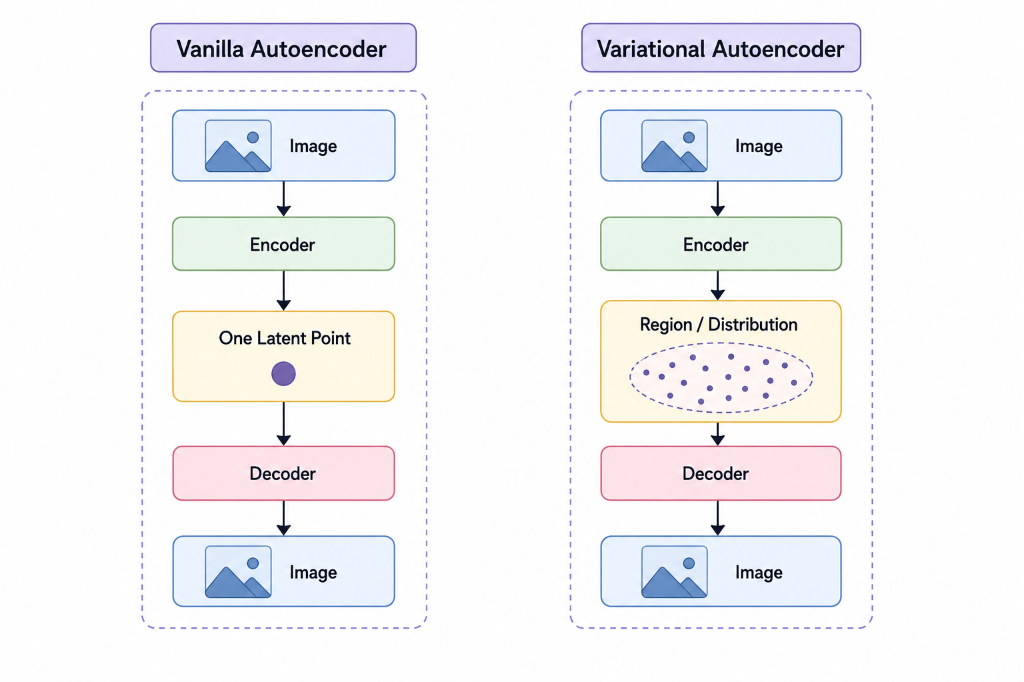
\includegraphics[width=0.85\linewidth]{figures/fig_8_vanilla_vs_vae.png}
    \caption{Comparison between Vanilla Autoencoders (mapping inputs to single isolated latent points) and Variational Autoencoders (mapping inputs to continuous probability distributions).}
    \label{fig:vanilla_vs_vae}
\end{figure}

\subsection{Why Probability Distributions?}
Consider representing a dog: every dog should not map to a single isolated point because dogs vary in color, size, posture, and breed, yet all belong to the concept of a dog. Instead of stating \emph{``this dog is exactly at point $(x,y)$''}, a VAE specifies \emph{``this dog belongs to a region centered around $\boldsymbol{\mu}$ with spread $\boldsymbol{\sigma}^2$''}.

A Gaussian latent region is fully defined by two parameter vectors produced by the encoder:
\begin{itemize}
    \item \textbf{Mean Vector ($\boldsymbol{\mu}$)}: The center of the region (most likely representation).
    \item \textbf{Log Variance Vector ($\log \boldsymbol{\sigma}^2$)}: The extent or radius of allowable variation.
\end{itemize}

\begin{figure}[htbp]
    \centering
    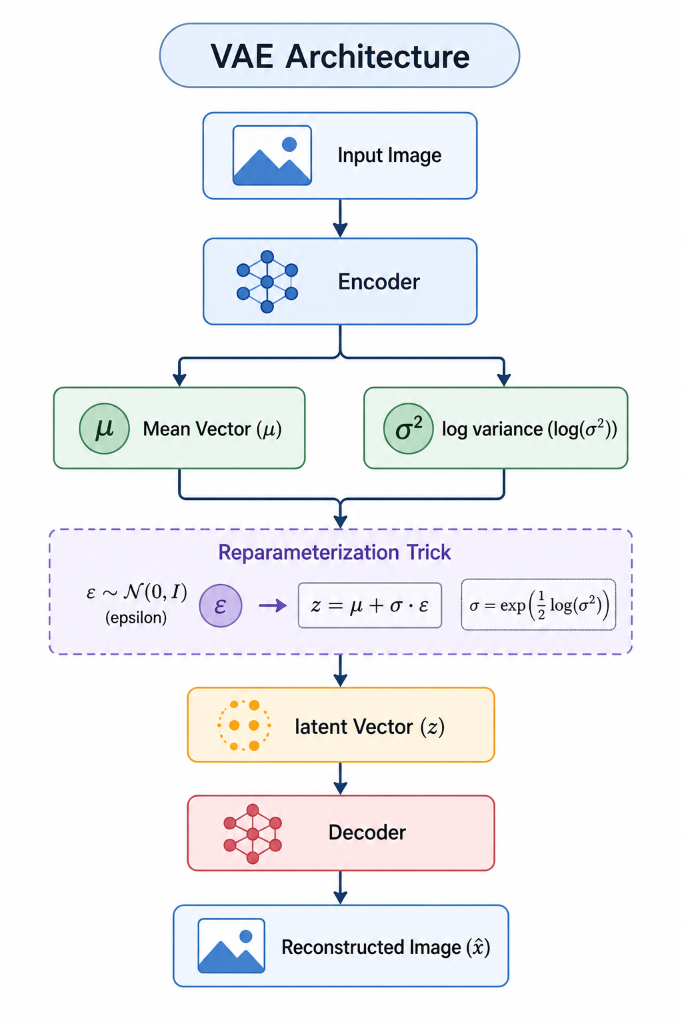
\includegraphics[width=0.85\linewidth]{figures/fig_8_vae_architecture.png}
    \caption{Detailed VAE Architecture incorporating the Reparameterization Trick to enable end-to-end backpropagation.}
    \label{fig:vae_architecture}
\end{figure}

\subsection{The Reparameterization Trick}

\subsubsection*{Why We Sample the Latent Vector}
We sample the latent vector $\mathbf{z}$ because we want the decoder to learn that an image is represented by an entire continuous region in the latent space rather than by a single fixed point. If we always used the mean vector $\boldsymbol{\mu}$ directly, every input would consistently produce the exact same latent representation, causing the model to behave similarly to a classical deterministic autoencoder.

By sampling different latent vectors $\mathbf{z}$ from the Gaussian distribution defined by $\boldsymbol{\mu}$ and $\boldsymbol{\sigma}^2$, the decoder learns to reconstruct valid images from many nearby points. This creates a smooth, continuous latent space where small changes in $\mathbf{z}$ lead to small changes in the generated image, enabling the VAE to generate novel and diverse samples.

\subsubsection*{Mathematical Formulation \& Gradient Flow}
However, directly sampling $\mathbf{z} \sim \mathcal{N}(\boldsymbol{\mu}, \boldsymbol{\sigma}^2)$ is a random operation, and random operations are non-differentiable, which blocks backpropagation. 

To solve this, VAE introduces the \textbf{Reparameterization Trick}. Instead of sampling $\mathbf{z}$ directly, we first sample independent standard Gaussian noise $\boldsymbol{\epsilon} \sim \mathcal{N}(0, \mathbf{I})$ and then compute the latent vector deterministically:
\[
\mathbf{z} = \boldsymbol{\mu} + \boldsymbol{\sigma} \odot \boldsymbol{\epsilon}
\]
This moves the randomness into $\boldsymbol{\epsilon}$, which is independent of the network, while $\boldsymbol{\mu}$ and $\boldsymbol{\sigma}$ remain differentiable outputs of the encoder. As a result, gradients flow through the encoder during backpropagation, allowing the entire VAE to be trained end-to-end.

\subsubsection*{Step-by-Step Execution Example}
Consider a concrete step-by-step example of passing a dog image through the VAE:
\begin{enumerate}
    \item \textbf{Encoder Prediction}: We feed the dog image into the encoder. Unlike a vanilla autoencoder, the encoder does not output one latent vector; instead, it outputs two parameter vectors:
    \[
    \boldsymbol{\mu} = [2.3, 1.8], \quad \boldsymbol{\sigma}^2 = [0.1, 0.2]
    \]
    The encoder indicates: \emph{``I think this dog belongs around here in the latent space, but I am not going to pick one exact point.''} Thus, we have a continuous region instead of a single isolated point.

    \item \textbf{Sampling $\mathbf{z}$ via Noise}: We need one latent vector to send to the decoder, but we do not use $\boldsymbol{\mu}$ directly. Instead, we first generate random noise from a standard Gaussian distribution, e.g., $\boldsymbol{\epsilon} = [0.4, -0.8] \sim \mathcal{N}(0, \mathbf{I})$. We then combine it with $\boldsymbol{\mu}$ and $\boldsymbol{\sigma}$ using $z = \boldsymbol{\mu} + \boldsymbol{\sigma} \odot \boldsymbol{\epsilon}$ to form the latent vector $\mathbf{z}$.

    \item \textbf{Decoder Reconstruction}: The decoder receives $\mathbf{z}$ and reconstructs the original dog image. Now, if we later pick a new point inside the region that the decoder has never seen before, it can still generate a realistic dog image.
\end{enumerate}

\section{Vector Quantized VAE (VQ-VAE)}

A \textbf{VQ-VAE} (Vector Quantized Variational Autoencoder, Van den Oord et al., 2017) replaces the continuous Gaussian latent space of a standard VAE with a \textbf{discrete Codebook}. The encoder still produces a continuous latent vector $z_e$, but it is immediately quantized by replacing it with the nearest codebook entry $z_q$. The decoder then reconstructs the image from this discrete representation.

This allows images to be represented as sequences of reusable \textbf{visual tokens} instead of arbitrary floating-point vectors, making VQ-VAE a foundational architecture for token-based generative models such as the original DALL-E and VQGAN.

\subsection*{Motivation: Continuous vs. Discrete Latent Spaces}
In a standard VAE, every image—even nearly identical images—maps to slightly different continuous latent points. For instance, subtle variations of a blue color might yield continuous vectors like:
\[
(124, 201, 87), \quad (124, 202, 88), \quad (125, 201, 86), \dots
\]
resulting in millions of redundant continuous possibilities.

The main idea of VQ-VAE is that instead of allowing arbitrary latent vectors, the encoder is forced to choose from a fixed, learned dictionary called a \textbf{Codebook}:
\begin{figure}[htbp]
    \centering
    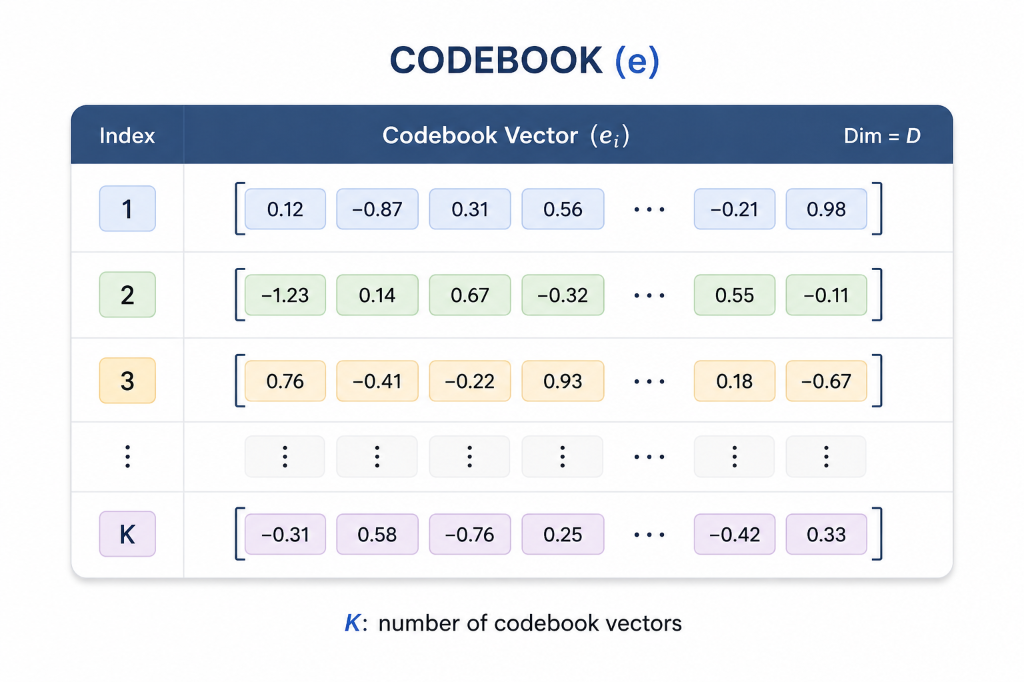
\includegraphics[width=0.85\linewidth]{figures/fig_8_codebook_table.png}
    \caption{Structure of the discrete Codebook $\mathcal{E}$ containing $K$ feature vectors of dimension $D$.}
    \label{fig:codebook_table}
\end{figure}

\begin{minipage}[t]{0.45\textwidth}
\begin{itemize}
    \item \textbf{Entry 1}: Round eye feature
    \item \textbf{Entry 2}: Green grass texture
    \item \textbf{Entry 3}: Blue sky
    \item \textbf{Entry 4}: Curved brown edge
\end{itemize}
\end{minipage}
\hfill
\begin{minipage}[t]{0.50\textwidth}
\vspace{0.3cm} % Move the text down
These semantic entry representations are not manually engineered; instead, they are discovered automatically by the model during end-to-end training.
\end{minipage}

\begin{figure}[htbp]
	\centering
	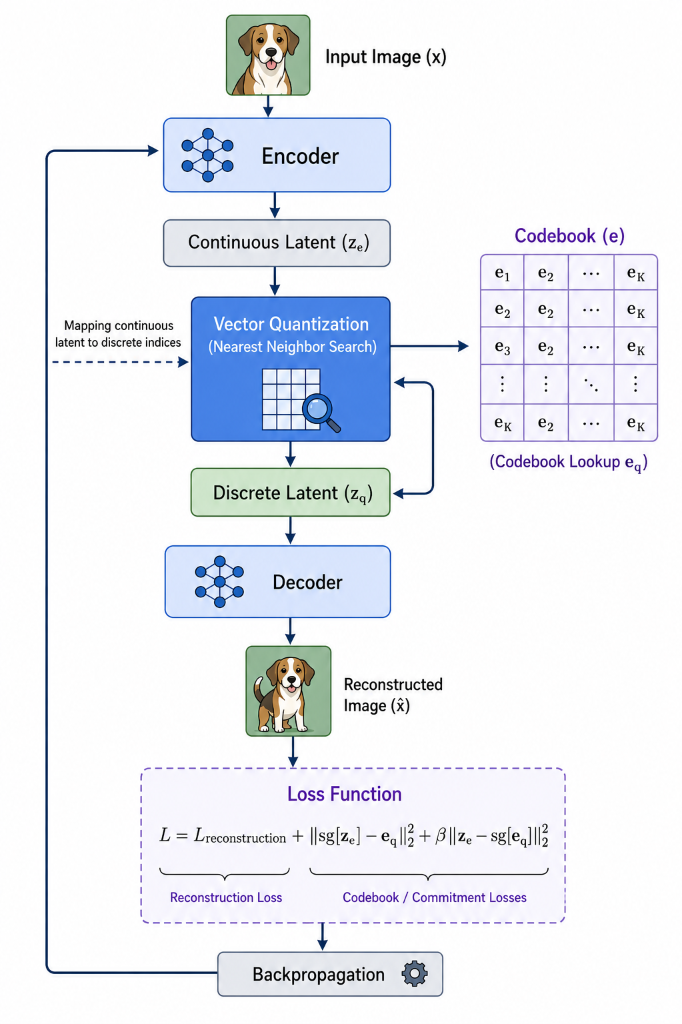
\includegraphics[width=0.85\linewidth]{figures/fig_8_vqvae_architecture.png}
	\caption{VQ-VAE Architecture showing Vector Quantization over a discrete codebook dictionary and loss formulation.}
	\label{fig:vqvae_architecture}
\end{figure}
\clearpage
\subsection{Vector Quantization Mechanism}
Instead of generating a single vector for an entire image, the encoder extracts spatial features and outputs a continuous latent vector $z_e(x)$ for each image patch. For each patch vector, the quantization layer searches the codebook dictionary $\mathcal{E} = \{e_1, e_2, \dots, e_K\}$ for the nearest vector entry in Euclidean distance:
\[
z_q(x) = e_k, \quad \text{where } k = \arg\min_j \| z_e(x) - e_j \|_2
\]



\subsubsection*{Example: From Image Patches to Discrete Visual Tokens}

Consider a dog image processed by a VQ-VAE. The quantization process converts each continuous latent feature into its nearest codebook entry.

\paragraph{Step 1. Continuous Latent Features}

After encoding, each spatial patch is represented by a continuous feature vector:

\[
\begin{array}{ccl}
\textbf{Patch 1} &:& (2.4,\;1.6)\;\rightarrow\;\text{Codebook Entry }81\\
\textbf{Patch 2} &:& (-1.1,\;0.8)\;\rightarrow\;\text{Codebook Entry }205\\
\textbf{Patch 3} &:& (0.5,\;1.2)\;\rightarrow\;\text{Codebook Entry }511\\
&\vdots&\\
\textbf{Patch N} &:& (1.7,\;0.1)\;\rightarrow\;\text{Codebook Entry }98
\end{array}
\]

Each continuous vector is replaced by the nearest prototype stored in the learned codebook.

\vspace{0.4cm}

\paragraph{Step 2. Image as a Sequence of Visual Tokens}

Instead of storing floating-point vectors, the image is represented only by the selected codebook indices:

\[
\boxed{
[81,\;205,\;511,\;\ldots,\;98]
}
\]

These indices are called \textbf{visual tokens}. Similar to how a sentence is represented by a sequence of words, an image can be represented by a sequence of discrete codebook entries.

\vspace{0.4cm}

\paragraph{Step 3. Quantization and Reconstruction}

Assume the encoder outputs

\[
z_e=[2.4,\;1.6].
\]

The nearest codebook vector is

\[
e_2=[2.6,\;1.5].
\]

The quantization layer performs

\[
z_q=e_2=[2.6,\;1.5].
\]

The original continuous representation is discarded, and only the quantized vector is forwarded to the decoder.

\vspace{0.3cm}

\begin{center}
\fbox{
\parbox{0.92\linewidth}{
\textbf{Key Idea}

The decoder never receives the encoder output $z_e$ directly. Instead, it reconstructs the image exclusively from the quantized representation $z_q$, ensuring that every latent feature belongs to the finite codebook.
}
}
\end{center}

\subsection{Loss Function \& Training Objective}
Because the $\arg\min$ operation in vector quantization is non-differentiable, straight-through gradient estimators are used. The total training objective combines reconstruction loss with codebook optimization and commitment penalties:
\[
\mathcal{L} = \mathcal{L}_{\text{reconstruction}} + \|\text{sg}[z_e] - e_q\|_2^2 + \beta \|z_e - \text{sg}[e_q]\|_2^2
\]
where $\text{sg}[\cdot]$ denotes the stop-gradient operator.
\begin{itemize}
    \item \textbf{Reconstruction Loss}: $\mathcal{L}_{\text{reconstruction}} = \|x - \hat{x}\|^2$ penalizes reconstruction errors.
    \item \textbf{Codebook Loss}: $\|\text{sg}[z_e] - e_q\|_2^2$ moves dictionary codebook vectors toward encoder outputs.
    \item \textbf{Commitment Loss}: $\beta \|z_e - \text{sg}[e_q]\|_2^2$ prevents encoder outputs from fluctuating wildly between dictionary entries.
\end{itemize}

\subsection*{Summary Comparison: VAE vs. VQ-VAE}
\begin{itemize}
    \item \textbf{Variational Autoencoder (VAE)}: The latent representation is \textbf{continuous} and obtained by sampling from a Gaussian probability distribution $\mathcal{N}(\boldsymbol{\mu}, \boldsymbol{\sigma}^2)$.
    \item \textbf{Vector Quantized VAE (VQ-VAE)}: The latent representation is \textbf{discrete} and obtained by selecting the nearest vector entry from a learned codebook dictionary.
\end{itemize}

\section{Denoising Autoencoders (DAE)}

In a vanilla autoencoder, the input and the target are identical. Researchers realized something critical: \emph{``The network might simply learn to copy the image.''} Even with a bottleneck, the model sometimes focuses on reconstructing low-level pixel details instead of learning robust features.

\subsection*{The Core Idea}
Instead of feeding the original clean image $x$, we feed a corrupted, noisy image $\bar{x}$:
\[
\bar{x} = x + \text{noise}
\]
\clearpage
\begin{figure}[htbp]
    \centering
    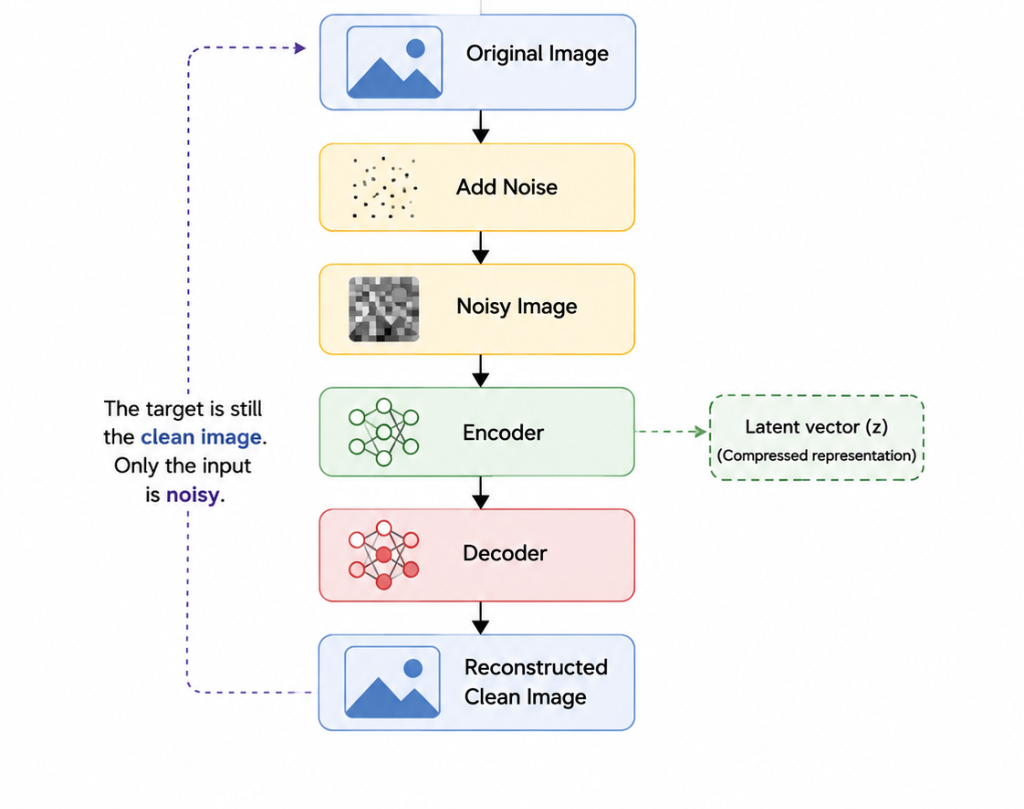
\includegraphics[width=0.85\linewidth]{figures/fig_8_denoising_autoencoder.png}
    \caption{Denoising Autoencoder pipeline: adding noise to clean inputs ($\bar{x} = x + \text{noise}$) and training the network to reconstruct the original clean target ($x$).}
    \label{fig:denoising_autoencoder}
\end{figure}



Mean Squared Error (MSE) loss and backpropagation are used to train the network. \textbf{Crucially, the target is still the clean image $x$; only the input is noisy ($\bar{x}$).}

\subsection*{Learning Robust Features}
Instead of memorizing raw pixels, the model learns meaningful representations:
\begin{itemize}
    \item Edges
    \item Shapes
    \item Textures
    \item Object structure
\end{itemize}
These learned features are significantly more useful for downstream tasks.

\subsection*{Connection to Diffusion Models}
Many modern generative architectures are based on exactly this denoising concept. The prominent example is \textbf{Diffusion Models}, which execute denoising via either of two equivalent targets:
\begin{center}
\begin{tabular}{ccc}
\fbox{\parbox{0.38\linewidth}{\centering \textbf{Noisy Image } ($\bar{x}$)\\[2pt]$\downarrow$\\[2pt]\textbf{Predict Clean Image } ($x$)}} & \quad $\mathbf{OR}$ \quad & \fbox{\parbox{0.38\linewidth}{\centering \textbf{Noisy Image } ($\bar{x}$)\\[2pt]$\downarrow$\\[2pt]\textbf{Predict Noise } ($\epsilon$)}}
\end{tabular}
\end{center}

\section{Sparse Autoencoders (SAE)}

If we have a latent vector containing 512 neurons, a vanilla autoencoder might produce activations like:
\[
z = [0.8, \; 0.4, \; 0.7, \; 0.3, \dots, 0.9]
\]
where almost every neuron is active. This means the network spreads information densely across many neurons. Researchers asked a fundamental question: \emph{``Can we force the network to represent each image using only a few important neurons?''}

\subsection*{Main Idea: Dense vs. Sparse Activations}
Instead of allowing all neurons to activate, a \textbf{Sparse Autoencoder} encourages most neurons to stay close to zero:
\begin{align*}
\text{Vanilla AE} &: [0.8, \; 0.4, \; 0.7, \; 0.3, \; 0.5, \; 0.9, \; 0.2] \\
\text{Sparse AE}  &: [0, \;\quad 0, \;\quad 1.2, \;\quad 0, \;\quad 0, \;\quad 0.8, \;\quad 0]
\end{align*}
Only a few neurons carry active information. For example, in recognizing a face: instead of every neuron contributing a small fraction to the entire image, individual neurons specialize in distinct feature concepts:
\begin{itemize}
    \item Eyes
    \item Nose
    \item Mouth
    \item Hair
    \item Beard
\end{itemize}
Because each neuron learns a specific concept, this leads to significantly more \textbf{interpretable} and \textbf{disentangled} representations.

\begin{figure}[htbp]
    \centering
    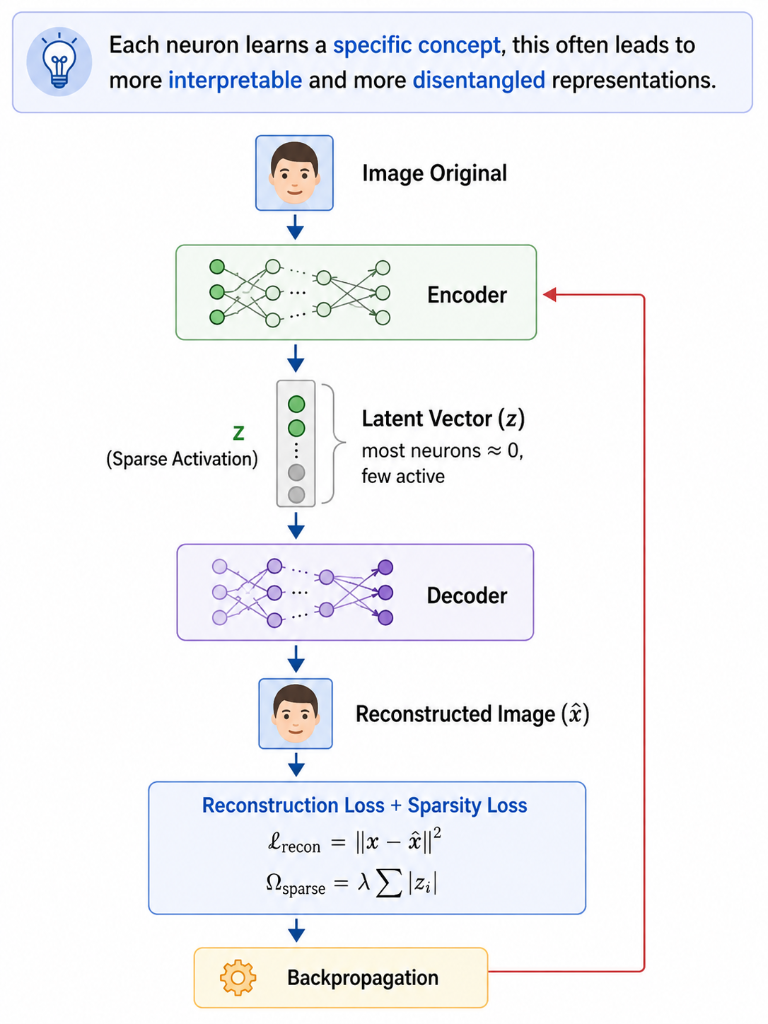
\includegraphics[width=0.85\linewidth]{figures/fig_8_sparse_autoencoder.png}
    \caption{Sparse Autoencoder architecture enforcing sparse latent activations where most neurons $\approx 0$ and only a few remain active.}
    \label{fig:sparse_autoencoder}
\end{figure}

\subsection{Objective Function \& Loss Formulation}
The reconstruction process is identical to a vanilla autoencoder; the primary difference lies in the loss function. Instead of minimizing only reconstruction error, we minimize the combined loss:
\[
\text{Total Loss} = \text{Reconstruction Loss} + \text{Sparsity Penalty}
\]
Formally, the total loss $\mathcal{L}_{\text{SAE}}$ combines standard reconstruction error with a sparsity penalty $\Omega_{\text{sparse}}(z)$:
\[
\mathcal{L}_{\text{SAE}} = \| x - \hat{x} \|^2 + \lambda \sum_i |z_i|
\]
The sparsity penalty discourages too many neurons from being active simultaneously. Common choices for the sparsity penalty include:
\begin{itemize}
    \item \textbf{$L_1$ Regularization}: Adds an $L_1$ norm penalty on latent activations $\sum_i |z_i|$.
    \item \textbf{KL Divergence}: Encourages a low average activation per neuron across training batches relative to a target sparsity parameter $\rho$.
\end{itemize}

\subsection*{Summary}
A Sparse Autoencoder has the same architecture as a vanilla autoencoder but adds a sparsity penalty to the loss function, encouraging only a small number of latent neurons to be active. This leads to compact, efficient, and highly interpretable feature representations.

\chapter{Generative Adversarial Networks (GANs)}

Before GANs, autoencoders and VAEs were major generative models. VAEs were a major breakthrough because they learned a continuous latent space, allowing them to generate new images by sampling latent vectors. However, they had a major drawback: the generated images were often blurry.

The main reason for this blur is the reconstruction loss, such as MSE or $L_1$ loss. During training, a VAE tries to reconstruct the original image pixel by pixel. When multiple outputs are possible, the safest way to minimize the reconstruction loss is to predict the average of all plausible images. Averaging pixels smooths edges and textures, producing blurry results.

Researchers realized that pixel similarity does not necessarily mean visual realism. Two real images of the same object can have very different pixel values because of lighting, pose, or background, yet both look perfectly realistic to humans.

This led to a new idea: instead of asking the model to reconstruct a specific image, ask it to generate an image that looks real. To achieve this, GANs introduced a second neural network called the discriminator, whose job is to distinguish real images from fake ones.

The generator learns to create fake images that fool the discriminator, while the discriminator learns to detect them. This competitive process is called adversarial learning.

The key innovation of GANs is that they optimize for realism rather than pixel accuracy, allowing them to generate much sharper and more realistic images than VAEs.

\begin{propertybox}[Summary: VAE vs. GAN]
\begin{itemize}
    \item \textbf{VAE}: Generates images using reconstruction loss $\rightarrow$ often blurry
    \item \textbf{Problem}: Pixel-wise losses encourage averaging, reducing image sharpness and blurring images
    \item \textbf{GAN Solution}: Replace reconstruction with adversarial learning
    \item \textbf{Generator}: Creates fake images
    \item \textbf{Discriminator}: Distinguishes real from fake images
    \item \textbf{Goal}: Generate images that look realistic enough to fool the discriminator
\end{itemize}
\end{propertybox}

\section{Vanilla GAN}

Unlike an autoencoder, a GAN does not have an encoder, a decoder, or a reconstruction loss. Instead, it has two completely different neural networks that compete against each other:
\begin{itemize}
    \item Generator ($G$)
    \item Discriminator ($D$)
\end{itemize}

This competition is what makes GANs unique.

\subsection*{I) The Generator}

The generator is responsible for creating images. Unlike an autoencoder, it does not receive an image; instead, it takes a random noise vector $z$ (usually sampled from a Gaussian distribution) and learns a mapping:

\[
z \longrightarrow \text{Generator} \longrightarrow \text{Fake Image}
\]

We start from random noise because we want the generator to create new images, not copy existing ones.

The input to the generator is usually written as $z \sim \mathcal{N}(0, 1)$, a random vector from a Gaussian distribution.
\[
z = [0.21, -1.34, 0.56, \dots]
\]
These numbers have no meaning. They are just random values. The generator's job is to transform meaningless noise into a realistic image.

\subsection*{II) The Discriminator}

The discriminator is a binary classifier. It receives either a real image from the dataset or a fake image generated by the generator and outputs the probability that the image is real.

\[
\text{Image} \longrightarrow \text{Discriminator} \longrightarrow \text{Probability} \longrightarrow \begin{cases} \text{Real} \\ \text{or} \\ \text{Fake} \end{cases}
\]

\begin{itemize}
    \item $0.98 \rightarrow 98\%$: This is likely a real image.
    \item $0.02 \rightarrow$: This image is almost certainly fake.
\end{itemize}

The discriminator receives two kinds of images:
\begin{itemize}
    \item \textbf{Real image}: These come directly from the training dataset.
    \item \textbf{Fake image}: These come from the generator.
\end{itemize}

The discriminator never knows which one it receives. Its only task is to answer: real or fake?

\subsection*{Architecture}

\begin{figure}[H]
\centering
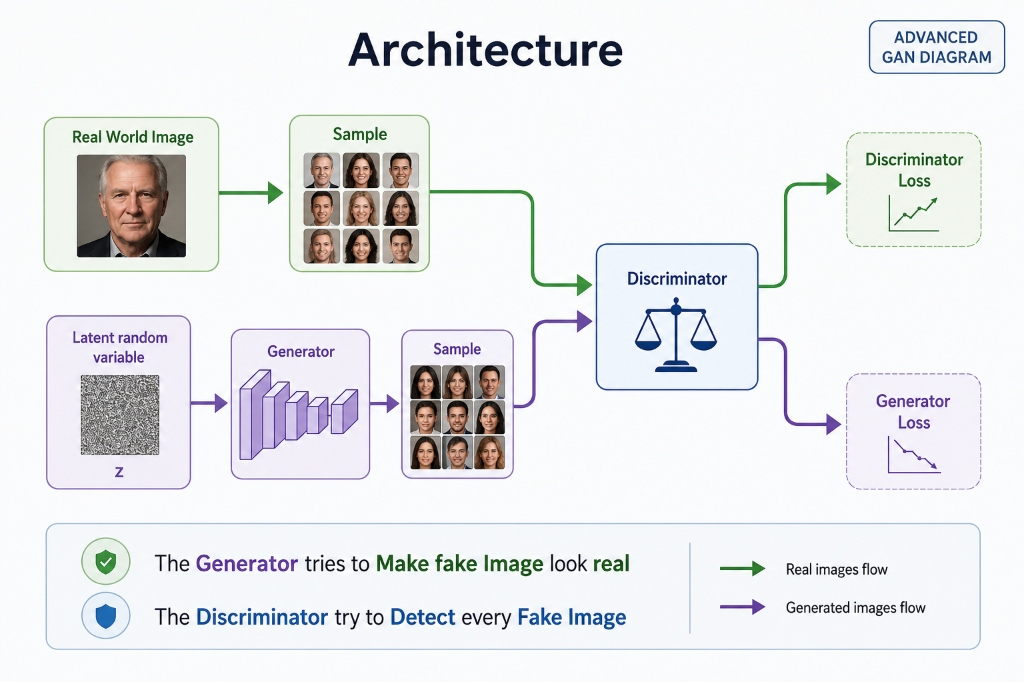
\includegraphics[width=0.88\textwidth]{figures/fig_9_1_advanced_gan_architecture.jpg}
\end{figure}

\begin{itemize}
    \item The \textbf{generator} tries to \textbf{make fake images look real}.
    \item The \textbf{discriminator} tries to \textbf{detect fake images}.
\end{itemize}

\section{The Training Process}

\begin{enumerate}
    \item Sample a batch of real images from the dataset.
    \item Sample a batch of random noise vectors $z$.
    \item Generate fake images using the generator:
    \[
    \text{Fake Images} = G(z)
    \]
    \item Train the Discriminator using:
    \begin{itemize}
        \item Fake images (from the generator) $\rightarrow$ target = fake ($0$)
        \item Real images $\rightarrow$ target = real ($1$)
        \item Update only the discriminator.
    \end{itemize}
    \item Sample another batch of random noise (or reuse the previous one).
    \item Generate fake images again $G(z)$
    \item Freeze the Discriminator's weights (so they are not updated)
    \item Pass the fake images through the discriminator.
    \item Update only the generator so that the discriminator classifies its fake images as real ($1$).
    \item Repeat.
\end{enumerate}

Generate fake images twice because the generator changes after every update:
\begin{itemize}
    \item The first fake batch is used to train the discriminator.
    \item The second fake batch is used to train the generator while the discriminator is frozen.
\end{itemize}

Some implementations reuse the same fake images, while others generate a new batch. Both approaches work; generating a new batch is common.

\subsubsection*{Training the Discriminator}

\begin{figure}[H]
\centering
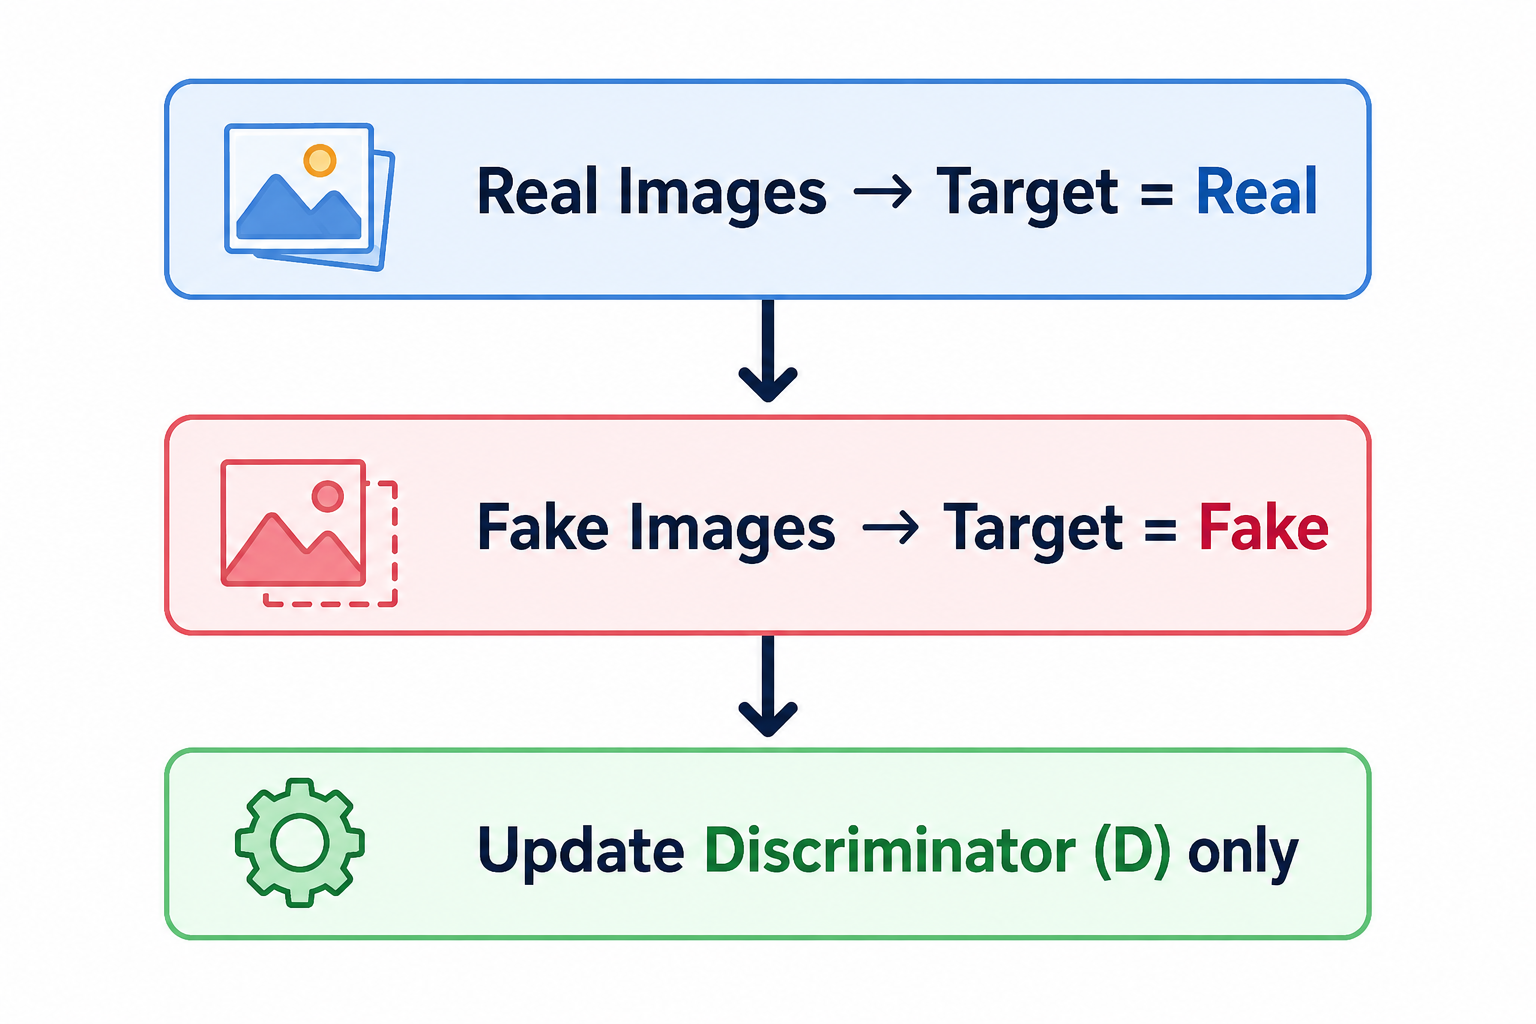
\includegraphics[width=0.85\textwidth]{figures/9-55 figure.png}

\end{figure} 
\clearpage
\subsubsection*{Training the Generator}
\begin{figure}[H]
\centering
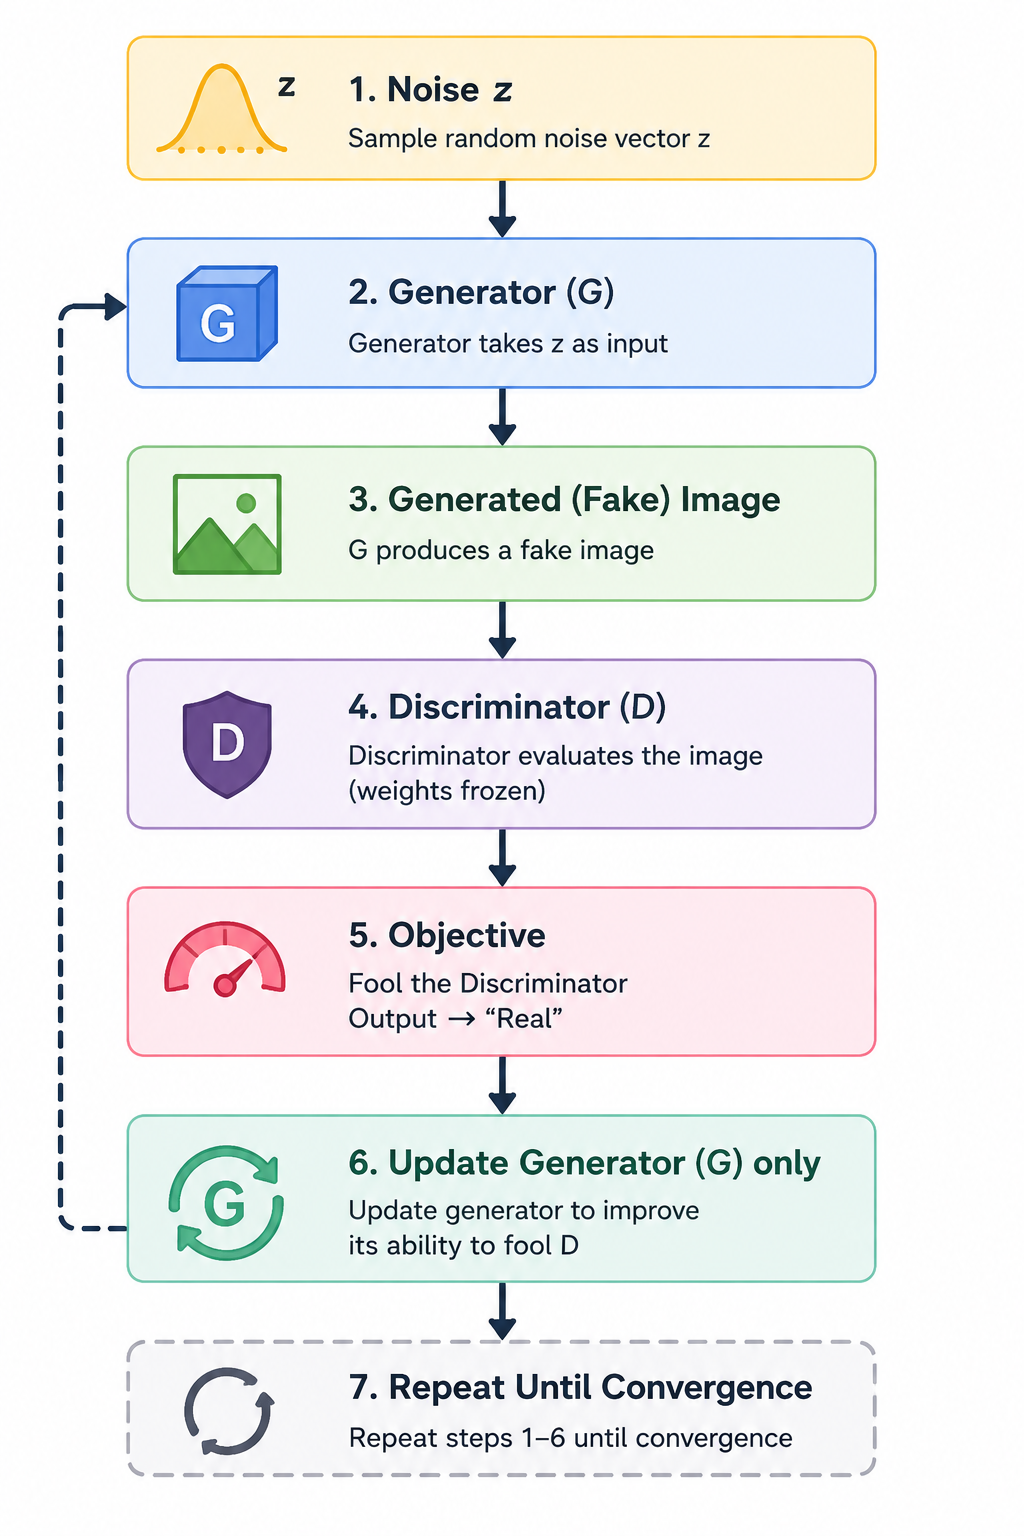
\includegraphics[width=0.85\textwidth]{figures/9-56 figure.png}
\end{figure}

The Generator is Powerful because is never told:
``The left eye should be two pixels higher''
or ``The hair color is wrong''

It receives only one signal: ``This image look fake''
From this simple feedback, it Gradually learns:
\begin{itemize}
    \item facial Structure
    \item lighting
    \item textures
    \item shadows
    \item Object shapes
    \item fine details
\end{itemize}

This is why GANs were able to Produce much sharper images than VAE.

\subsection*{Minimax Game}

GAN Training is formulated as a minimax Game:
\[
\min_G \max_D V(D, G)
\]

\begin{itemize}
    \item Discriminator ($\max_D$) tries to maximize its ability to distinguish real from fake.
    \item Generator ($\min_G$) tries to minimize The Discriminator's success by generating more realistic images.
\end{itemize}

Each network improves by Competing against the other, which is why GANs are called adversarial.

\subsection*{Nash Equilibrium}

The Ideal outcome is The Nash Equilibrium, where:
\begin{itemize}
    \item The Generator produces images indistinguishable from real ones.
    \item The Discriminator Cannot do better than random guessing and outputs approximately $0.5$ for both real and fake images.
\end{itemize}

At this point, neither network can improve its performance without the other changing as well.

In Practice, GANs rarely reach this Perfect balance. One network often becomes stronger than The other, leading To training instability. If the Discriminator becomes too accurate too early, The Generator receives very small gradients (the Vanishing Gradient Problem) and Stop improving. These difficulties Motivated The development of improved GAN variants such as DCGAN, WGAN and StyleGAN.

\section{Why GANs Are Hard to Train}

When GANs were introduced in 2014, they produced amazing images.
But researchers Quickly discovered something frustrating: Training a GAN is much harder than training a CNN, a transformer, or an Autoencoder.
Sometimes it works beautifully. At other times, with the same architecture and almost the same hyperparameters, training completely fails. Why?
Because two neural networks are learning simultaneously, and each one changes the learning environment of the other, making Optimization unstable.

\subsection*{The Four Main Problems}

\subsubsection*{1) Vanishing gradients}
\begin{itemize}
    \item if The Discriminator becomes too good, it Confidently Classifies fake image as fake
    \item The sigmoid output saturates near $0 \sim 0.001$ (fake) or $1$ (real), producing very Small Gradients
    \item As a Result, The Generator receives almost no useful feedback and Stop Learning
\end{itemize}

\subsubsection*{2) Mode Collapse (The most GAN Problem)}

Suppose Our Dataset contains $\begin{cases} \text{- Cats} \\ \text{- Dogs} \\ \text{- Cars} \\ \text{- Birds} \end{cases}$

The Generator should learn all of Them.
If the generator produces a dog image every time, the discriminator is fooled.
The Generator realizes: why should I Generate any thing else?
It starts producing $\text{dog} \rightarrow \text{dog} \rightarrow \text{dog} \dots \rightarrow \text{dog}$ with tiny variations. The generator has found an easy way to fool the discriminator; this phenomenon is called mode collapse.
\begin{itemize}
    \item Instead of learning the entire data distribution (ex: dogs, cats, cars, Birds), The Generator discovers a few Outputs that Consistently fool the Discriminator.
    \item It repeatedly generates only those samples with small variations, ignoring the rest of The data
\end{itemize}

\subsubsection*{3) Oscillation}

Today: the generator learns how to create good cats \\
$\phantom{today:\ }$ the Discriminator adapts \\
Tomorrow: the generator switches to dogs \\
$\phantom{tomorrow:\ }$ the Discriminator adapts again \\
$\phantom{tomorrow:\ } \quad \Downarrow$ \\
$\phantom{tomorrow:\ } \text{Birds} \rightarrow \text{Cats} \rightarrow \text{Dogs} \dots$

The Generator keeps chasing the Discriminator:
\begin{itemize}
    \item The Generator and Discriminator Continually adapt to each other
    \item The Generator may learn to Generate one type of image, The Discriminator adapts, then The Generator Switches to another type
    \item This cycle repeats without reaching a Stable Solution
\end{itemize}

\subsubsection*{4) Imbalanced Learning}
\begin{itemize}
    \item If the Discriminator learns much faster than the Generator, the Generator receives almost no useful Gradients.
    \item If The Generator becomes too Strong, The Discriminator can no longer learn effectively.
    \item Successful GAN training requires both networks to improve at approximately the Same rate.
\end{itemize}

The Original GAN demonstrated that adversarial Learning Could generate highly realistic images, But it Training is inherently unstable due to Vanishing gradients, Mode collapse, oscillation, and Imbalanced Learning. Nearly every later GAN architecture was designed to Address These optimization Challenges while Preserving the Core Generator-versus-Discriminator framework.

\section{DCGAN (Deep Convolutional GAN) (2015)}

Before DCGAN, people Knew GANs worked in Theory but training them on real images was difficult and unstable.
In 2015, DCGAN showed that simply changing the architecture Could dramatically improve image Quality and Training stability.

DCGAN was the first GAN Architecture specifically designed for Image Generation. Instead of Using fully Connected layers like the Original GAN, DCGAN uses Convolutional Neural Network (CNNs), making Training more stable and improving image Quality.

The Original GAN used dense layers, which:
\begin{itemize}
    \item Scale poorly to large images
    \item Ignore spatial relationships between neighboring pixels
    \item Produce lower-Quality images and unstable Training
\end{itemize}

DCGAN solved these issues by replacing dense layers with Convolution-based architecture.

\subsection*{I) Generator Architecture}

The Generator starts from a random noise vector $z$ and progressively increases the image resolution using Transposed Convolution (\textbf{ConvTranspose}).

Each transposed convolution upsamples the feature maps, gradually constructing the final image.

\textbf{why Transposed}: Convolution usually reduces spatial dimensions. $64\times64 \rightarrow \text{Conv} \rightarrow 32\times32$.
A transposed Conv does the opposite: It upsamples the feature maps.
example: $4\times4 \rightarrow \text{TransConv} \rightarrow 8\times8 \rightarrow \text{TransConv} \rightarrow 16\times16\dots$

\begin{figure}[H]
\centering
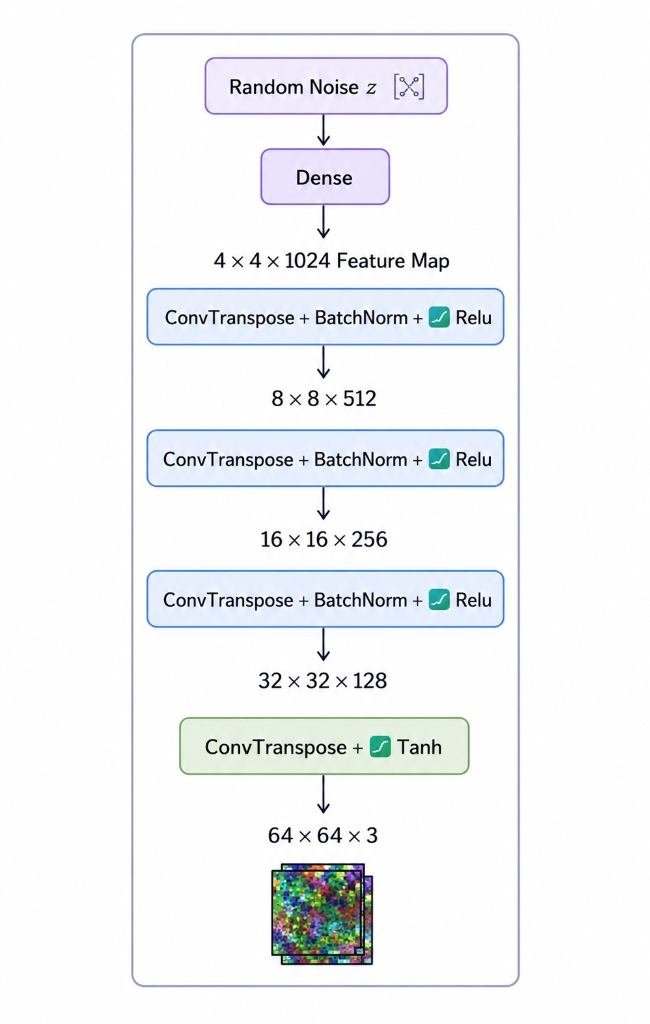
\includegraphics[width=0.88\textwidth]{figures/fig_9_2_dcgan_generator_architecture.jpg}
\end{figure}

\subsection*{II) Discriminator Architecture}

The Discriminator is the mirror of the Generator. It progressively reduces the image size using standard Convolutions, extracts features, and outputs the probability that the image is real.

\begin{figure}[H]
\centering
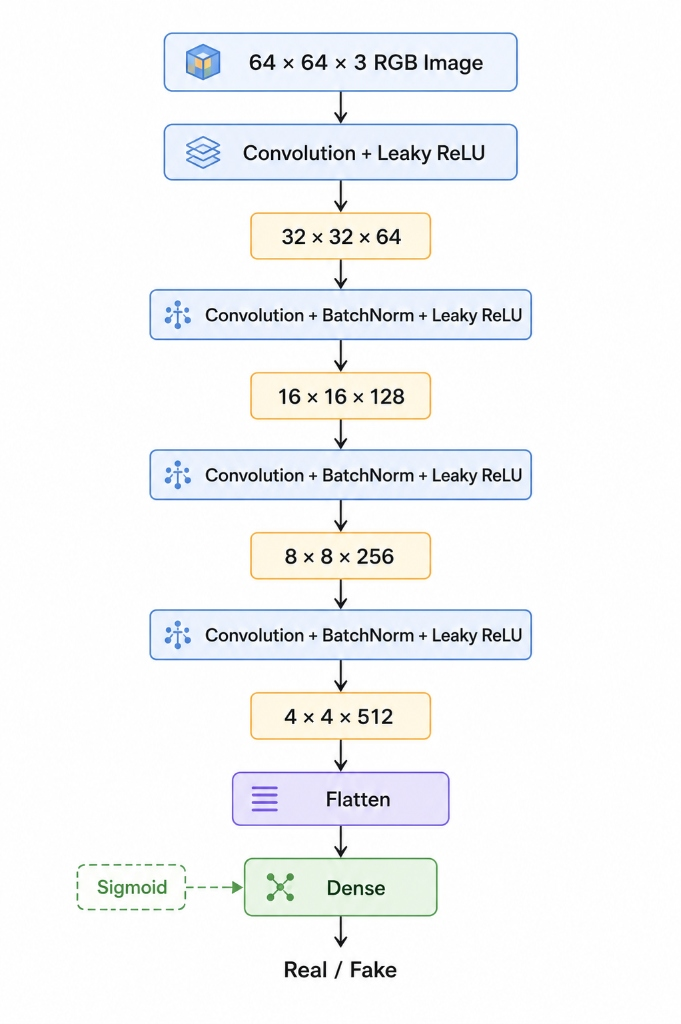
\includegraphics[width=0.88\textwidth]{figures/fig_9_3_dcgan_discriminator_architecture.jpg}
\end{figure}

\subsection*{Overall DCGAN Pipeline}

\begin{figure}[H]
\centering
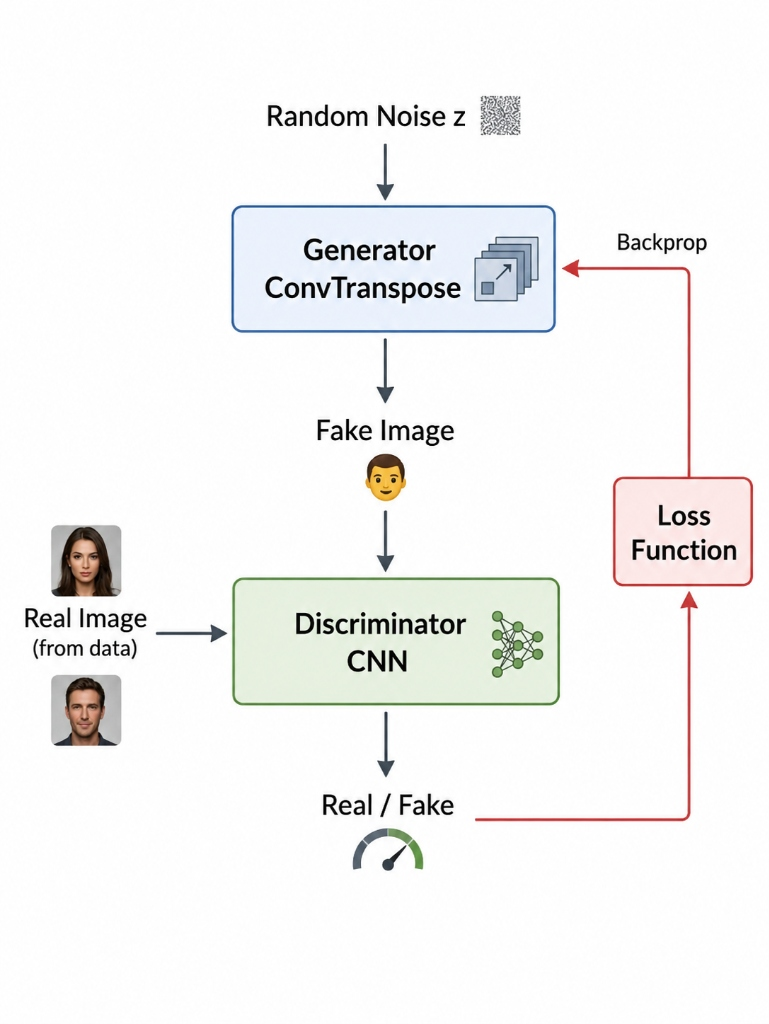
\includegraphics[width=0.88\textwidth]{figures/fig_9_4_overall_dcgan_pipeline.jpg}
\end{figure}

\subsection*{Batch Normalization}

The Original GAN often suffered from unstable Training because activations could change dramatically during optimization, DCGAN introduced Batch Normalization in most layers, BatchNorm helps by:
\begin{itemize}
    \item Stabilizing activations
    \item Speeding up training
    \item making gradient flow more smoothly
\end{itemize}

This does not solve every GAN problem, but it makes optimization much easier.

\subsection*{Leaky ReLU}

The discriminator uses Leaky ReLU instead of ReLU because Leaky ReLU allows a small negative slope. The neuron still receives gradients, which prevents it from stopping learning and improves training stability.

\subsection*{Why Tanh at the Generator Output?}

The generator uses Tanh as its final activation because it outputs pixel values in the range $[-1, 1]$. Therefore, the real training images are also normalized to $[-1, 1]$ so that both real and generated images have the same value range. Matching these ranges helps stabilize training and improves convergence.

\subsection*{DCGAN Design Rules}

\begin{itemize}
    \item Replace pooling layers with strided convolutions (discriminator) and transposed convolutions (generator)
    \item Use Batch Normalization in most layers
    \item Use ReLU in the generator (except the output layer)
    \item Use Leaky ReLU in the discriminator
    \item Use Tanh at the generator output
    \item Remove unnecessary fully connected hidden layers.
\end{itemize}

These simple rules dramatically improved training compared with the original GAN.

DCGAN did not change the adversarial loss. The generator and discriminator still play the same minimax game. The main improvement is the architecture, not the objective.

\section{cGAN Conditional GANs (2016)}

A vanilla GAN generates images randomly.
\[
\text{Noise } (z) \longrightarrow \text{Generator} \longrightarrow \text{Random Image}
\]

We cannot control whether the output is a dog, cat, car, or house. Imagine asking a GAN, ``Generate a cat.'' It cannot; it only maps noise to images.

A conditional GAN (cGAN) adds extra information (a condition) to both the generator and the discriminator. Usually, the condition is a class label.

Researchers asked: what if we also give the Generator the class label?
Instead of Noise $\rightarrow$ Generator $\rightarrow$ Image, we use:
\[
\text{Noise} + \text{Label} \longrightarrow \text{Generator} \longrightarrow \text{Image}
\]

Now the generator knows:
\begin{itemize}
    \item The random appearance ($z$)
    \item The desired category (label)
\end{itemize}

\subsection*{Generator}

Instead of receiving only $z$, the generator receives $(z, y)$, where $z = \text{random noise}$ and $y = \text{label}$.

\[
z + \text{Label} = \text{dog} \longrightarrow \text{Generator} \longrightarrow \text{Random dog}
\]

\begin{itemize}
    \item The label controls what is generated.
    \item The noise controls how it looks.
\end{itemize}

Why keep the noise? Suppose the generator receives only ``dog.'' Then every output would become dog A, dog A, dog A: always the same dog.
The noise introduces diversity:
\[
\left.
\begin{array}{l}
z_1 + \text{Dog} \longrightarrow \text{Dog a} \\
z_2 + \text{Dog} \longrightarrow \text{Dog b} \\
z_3 + \text{Dog} \longrightarrow \text{Dog c}
\end{array}
\right\} \quad \text{Same class, different appearance}
\]

\subsection*{Discriminator}

The discriminator now receives an image plus a label. Instead of asking ``real or fake?'', it asks, ``Is this image real for this label?''
Even if the image is real, the discriminator rejects it when it does not match the condition.

\begin{figure}[H]
\centering
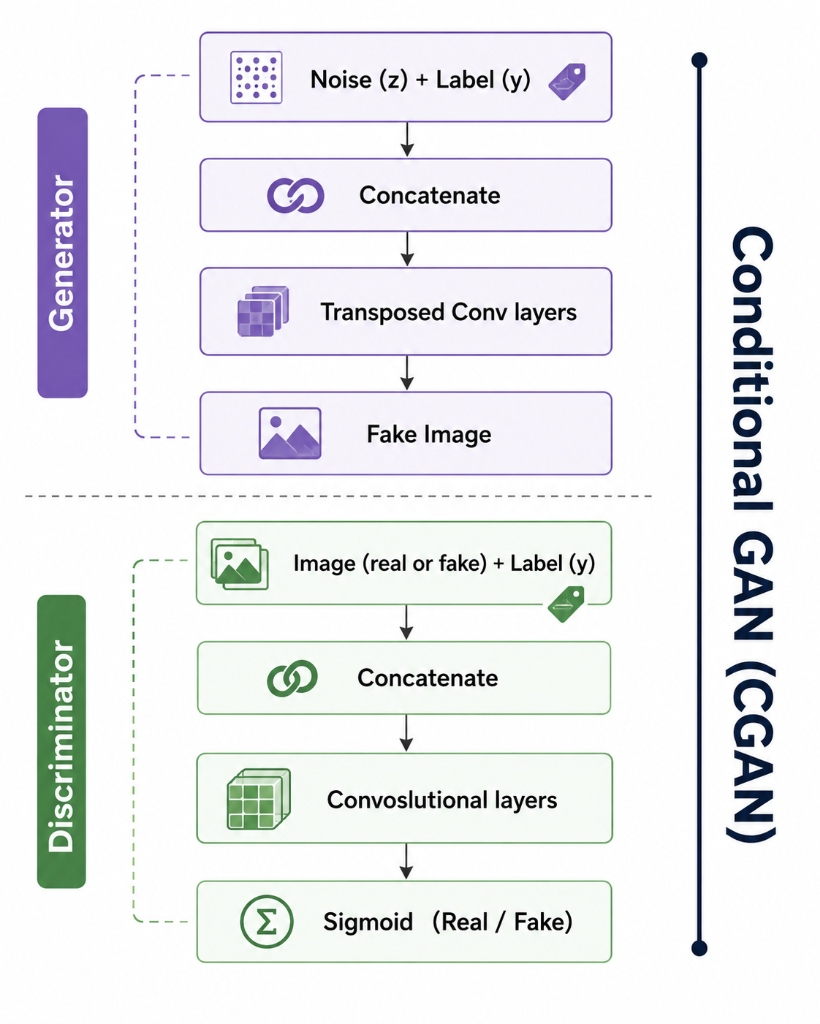
\includegraphics[width=0.88\textwidth]{figures/fig_9_5_cgan_architecture.jpg}
\end{figure}

\subsection*{Training Flow}

\begin{enumerate}
    \item Choose a label $y$ (ex: dog)
    \item Sample random noise $z$.
    \item Generator: $(z, y) \rightarrow \text{fake dog}$.
    \item Discriminator: $(\text{real dog}, y) \rightarrow \text{real}$.
    \item Discriminator: $(\text{fake dog}, y) \rightarrow \text{fake}$.
    \item Update the discriminator.
    \item Freeze the discriminator.
    \item Generate another fake dog using $(z, y)$.
    \item Update the generator so the discriminator predicts ``real.''
    \item Repeat
\end{enumerate}

\subsection*{Applications}

\begin{itemize}
    \item Image Generation
    \item Image Colorization
    \item Super Resolution
    \item Semantic Image Generation
\end{itemize}

\section{Pix2Pix}

Pix2Pix is one of the most influential Conditional Generative Adversarial Networks (cGANs). Instead of conditioning the generator on a class label, Pix2Pix conditions both the generator and discriminator on an input image. The model learns a mapping from the input image to a corresponding output image, enabling \textbf{image-to-image translation} tasks such as image colorization, semantic segmentation, edge-to-photo synthesis, and style transformation.

\subsection*{Limitation of Pix2Pix}


\section{CycleGAN: Unpaired Image-to-Image Translation (2017)}

Unlike models that require fully paired and matched data (such as Pix2Pix), CycleGAN enables us to learn from completely independent datasets. In many real-world applications, collecting such paired data is nearly impossible, which is why CycleGAN comes as an alternative solution.

Instead of relying on precise matching between images, CycleGAN learns from two independent and distinct sets of images:
\begin{itemize}
    \item \textbf{Domain A (Dataset 1)}: e.g., Horse Domain
    \item \textbf{Domain B (Dataset 2)}: e.g., Zebra Domain
\end{itemize}

\begin{figure}[H]
\centering
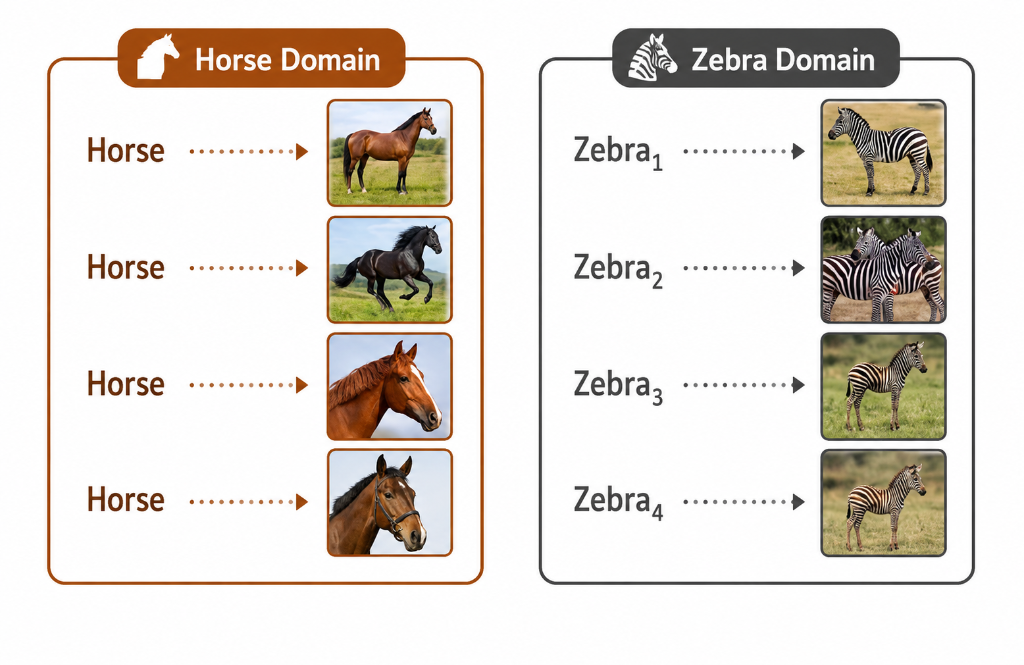
\includegraphics[width=0.85\textwidth]{figures/fig_9_12_cyclegan_domains.png}
\caption{Unpaired Domain Mapping: Horse Domain ($X$) vs. Zebra Domain ($Y$).}
\label{fig:cyclegan_domains}
\end{figure}

Thus, the model only knows that these images belong to the Horse Domain and those images are associated with the Zebra Domain.

\subsection*{Dual Generator and Discriminator Architecture}

Suppose we have a Horse image and Generator $G$ turns it into a Zebra. But how do we know if it looks like a Zebra while preserving the pose, background, and shape of the original horse? It could generate any random Zebra!

Solution: CycleGAN introduces two Generators instead of one:
\begin{itemize}
    \item \textbf{Generator $G$}: Learns the mapping from Domain A to Domain B ($A \rightarrow B$, e.g., Horse $\rightarrow$ Zebra).
    \item \textbf{Generator $F$}: Learns the mapping from Domain B to Domain A ($B \rightarrow A$, e.g., Zebra $\rightarrow$ Horse).
    \item \textbf{Discriminator $D_B$}: Evaluates whether an image in Domain B is real or generated by $G$.
    \item \textbf{Discriminator $D_A$}: Evaluates whether an image in Domain A is real or generated by $F$.
\end{itemize}

\begin{figure}[H]
\centering
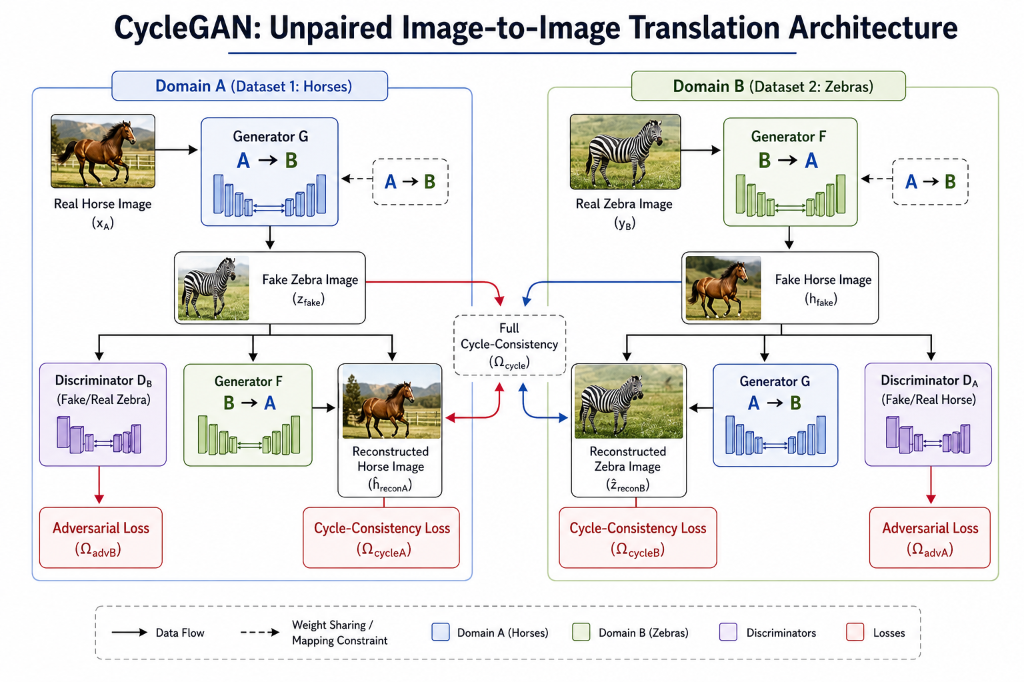
\includegraphics[width=0.92\textwidth]{figures/fig_9_13_cyclegan_architecture.png}
\caption{CycleGAN Complete Dual-Generator Architecture and Loss Interactions.}
\label{fig:cyclegan_arch}
\end{figure}

\subsection*{Cycle Consistency}

First, an image from Domain A is translated by Generator $G$ into a fake image in Domain B. Instead of stopping there, this generated image is passed through Generator $F$ to translate it back into Domain A. If the translation is meaningful, the reconstructed image should closely resemble the original input.

In other words, translating an image from one domain to another and then back again should recover the original image. The same process is performed in the opposite direction (Domain B $\rightarrow$ Domain A $\rightarrow$ Domain B).

By minimizing the difference between the original and reconstructed images, CycleGAN encourages the generators to preserve the content, structure, and identity of the image while changing only the domain-specific characteristics, allowing image-to-image translation without requiring paired training examples.

\subsection*{Why Does Cycle Consistency Work?}

Imagine we hire a translator: $\text{English} \longrightarrow \text{French} \longrightarrow \text{English}$. If the final English sentence is very different, the translation was poor. But if we recover almost the same sentence, the translation preserved the meaning. CycleGAN applies exactly the same principle to images.

Before CycleGAN, image-to-image translation required expensive paired datasets. CycleGAN showed that consistency is enough. Instead of saying ``this horse corresponds to this zebra'', it says ``if I translate there and back, I should recover the original.''

That simple idea removed the need for paired training examples.

\subsection*{CycleGAN Training Pipeline}

\begin{figure}[H]
\centering
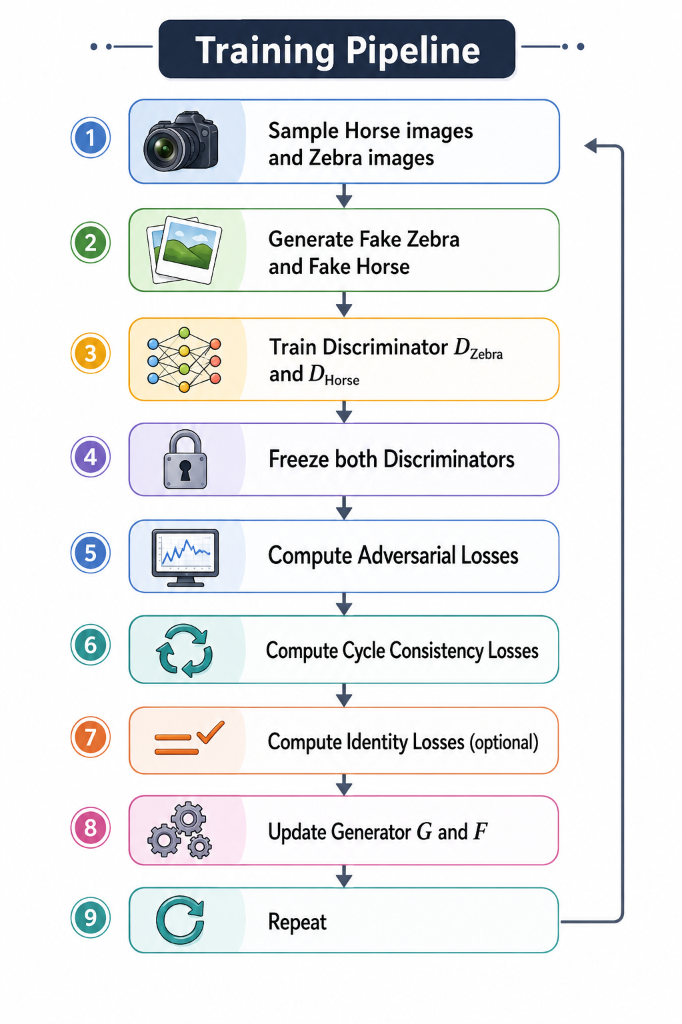
\includegraphics[width=0.78\textwidth]{figures/fig_9_14_cyclegan_pipeline.png}
\caption{CycleGAN Step-by-Step Training Pipeline.}
\label{fig:cyclegan_pipeline}
\end{figure}

This alternating process enables CycleGAN to learn realistic unpaired image-to-image translations while preserving original image content through Cycle Consistency.

\subsection*{The Three Losses in CycleGAN}

Unlike a vanilla GAN, CycleGAN does not rely on a single loss function; it combines three objectives:

\subsubsection*{1) Adversarial Loss}

Exactly like a normal GAN, Generator $G$ tries to fool the Zebra Discriminator ($D_B$), and Generator $F$ tries to fool the Horse Discriminator ($D_A$).

\subsubsection*{2) Cycle Consistency Loss}

This is the core loss:
\[
\text{Horse} \longrightarrow \text{Zebra} \longrightarrow \text{Horse} \approx \text{Original Horse}
\]
The reconstructed horse should remain close to the input image $x$:
\[
F(G(x)) \approx x \quad \text{and} \quad G(F(y)) \approx y
\]
\[
\mathcal{L}_{\text{cyc}}(G, F) = \mathbb{E}_{x \sim P_{\text{data}}(x)}[\|F(G(x)) - x\|_1] + \mathbb{E}_{y \sim P_{\text{data}}(y)}[\|G(F(y)) - y\|_1]
\]

\subsubsection*{3) Identity Loss (Optional but Very Useful)}

Identity loss teaches the generator not to change an image that is already in the target domain.

Generator $G$ is trained to convert Horse $\rightarrow$ Zebra. Now imagine that during training, we purposely give Generator $G$ a Zebra instead of a Horse. What should the output be?
\[
\text{Zebra} \longrightarrow \text{Generator } G \longrightarrow \text{Zebra}
\]
By passing a Zebra into Generator $G$, we are basically telling the Generator: ``This image is already in your target domain. Don't touch it.''

Identity loss helps preserve color composition and visual tone across domain translations.

\subsection*{Limitations of CycleGAN}
\begin{enumerate}
    \item \textbf{Cannot change geometry well}: It works best when the two domains have similar shapes (e.g., Horse $\rightarrow$ Zebra $\checkmark$, but Cat $\rightarrow$ Airplane $\times$).
    \item \textbf{May change important details}: It can unintentionally modify background colors or object identity.
    \item \textbf{Cycle consistency is not a guarantee}: An image can satisfy the cycle loss while still producing an unrealistic translation.
    \item \textbf{Training is slow and unstable}: It trains two generators and two discriminators simultaneously, making optimization difficult.
    \item \textbf{Requires enough data from both domains}: Although paired images are unnecessary, we still need a large collection of images from each domain.
\end{enumerate}

\begin{itemize}
    \item \textbf{Strength}: No paired dataset is required.
    \item \textbf{Weakness}: It struggles with large structural changes and still inherits the training instability common to GANs.
\end{itemize}

\section{StyleGAN (2019)}

In a normal GAN, the random latent vector $z$ is fed directly into the Generator to produce an image. Ideally, changing one part of $z$ should modify only one visual attribute, such as hair color or age. However, this is not what happens in practice. The latent space is \textbf{entangled}, meaning that information for different attributes is mixed together.

As a result, a small change in $z$ can simultaneously affect several characteristics of the generated image, such as age, hairstyle, lighting, face, or even background.

\begin{figure}[H]
\centering
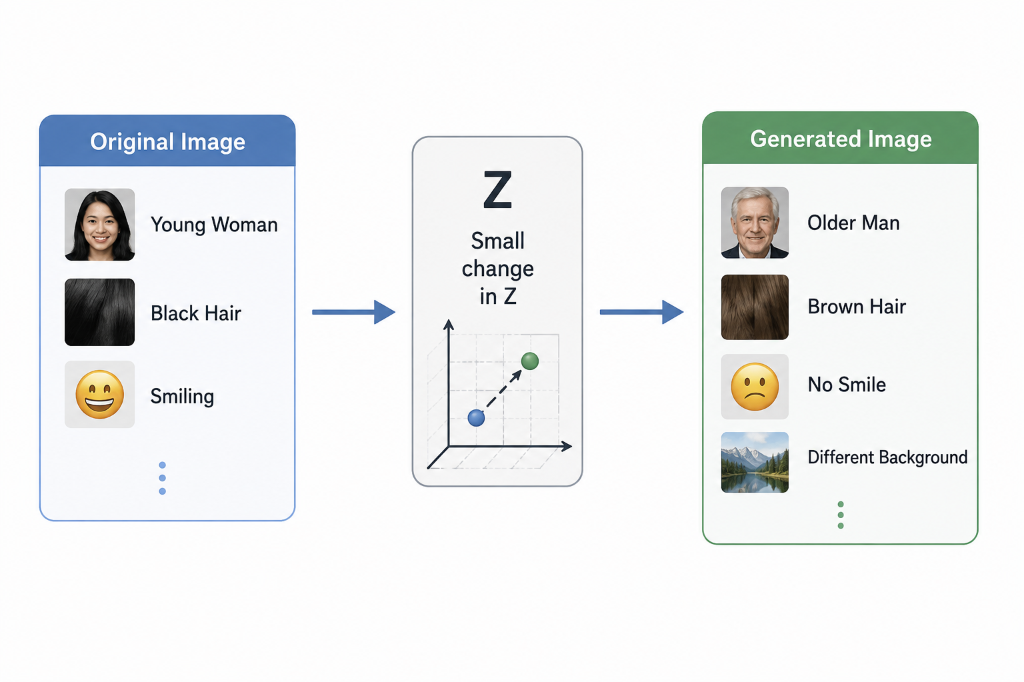
\includegraphics[width=0.85\textwidth]{figures/fig_9_11_latent_space_z.png}
\caption{Entangled Latent Space $Z$: Small changes in $Z$ affect multiple unrelated visual attributes.}
\label{fig:latent_z}
\end{figure}

Instead of changing only one attribute, many unrelated attributes change together. This lack of independent control makes it difficult to edit generated images in a meaningful and predictable way. StyleGAN was designed to solve this problem by learning a more \textbf{disentangled latent space}, where different directions correspond to different visual attributes.

\subsection*{StyleGAN: Key Innovations (2019)}

\textbf{The Main Idea}: Instead of sending $z$ directly into the Generator, StyleGAN first transforms it.

\begin{figure}[H]
\centering
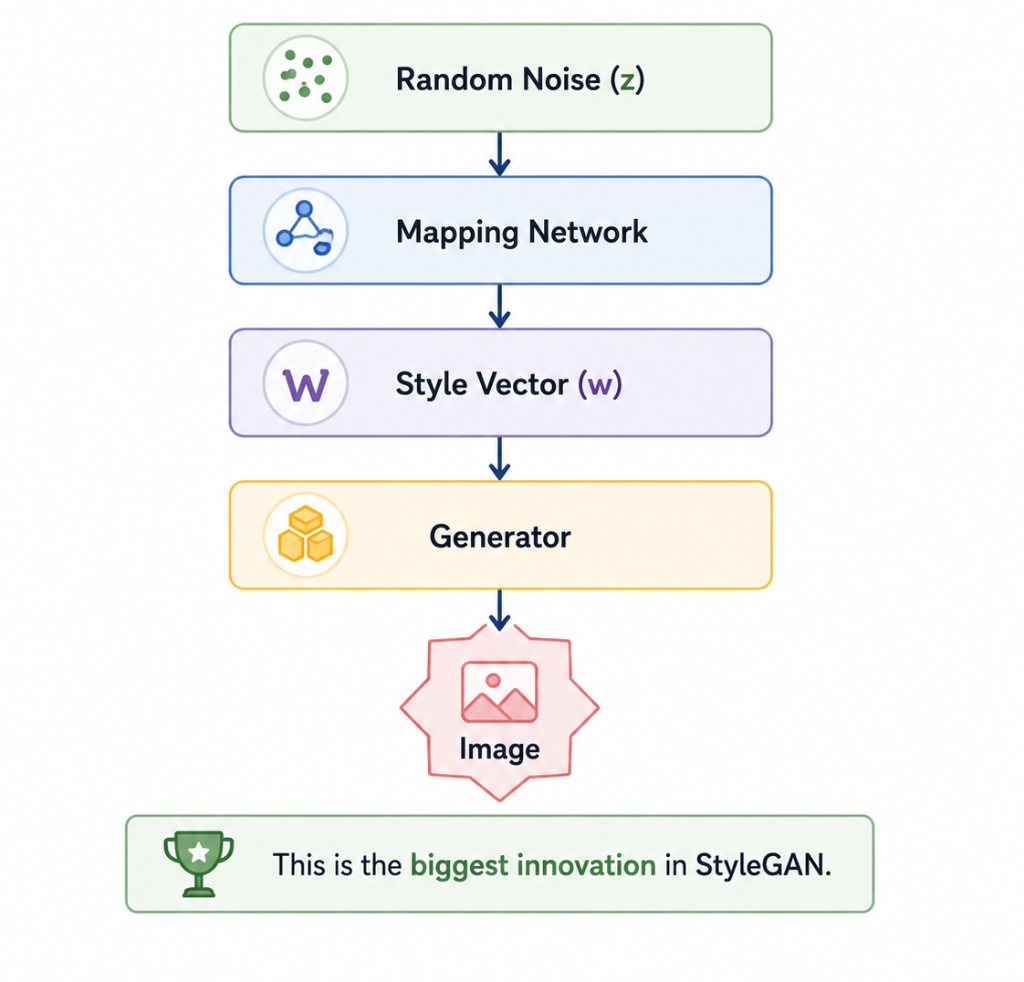
\includegraphics[width=0.82\textwidth]{figures/fig_9_7_stylegan_mapping_network.png}
\caption{StyleGAN Mapping Network ($z \rightarrow w$) Innovation.}
\label{fig:stylegan_mapping}
\end{figure}

This is the biggest innovation in StyleGAN.

\subsection*{I) Mapping Network}

The Mapping Network is a small MLP (typically 8 fully connected layers). Its job is:
\[
z \longrightarrow \text{Mapping Network} \longrightarrow w
\]
Where $z$ is the original random latent vector, and $w$ is the new latent representation.

$z$ comes from a simple Gaussian distribution $z \sim \mathcal{N}(0, I)$. Nothing in this distribution specifies separate dimensions (e.g., dimension 5 for hair color, dimension 12 for smile). The Generator must learn everything at once. The Mapping Network reorganizes this space into one that is easier for the Generator to use.

The goal is to make $w$ much more disentangled: instead of mixing all attributes together, different directions in $w$ tend to correspond to meaningful visual properties like age, hairstyle, pose, or facial expression.

\subsection*{II) Adaptive Instance Normalization (AdaIN)}

This is the second major innovation. Instead of using the same feature statistics for every generated image, \textbf{AdaIN} modifies the feature maps according to the style vector $w$. This allows each layer of the Generator to control different visual attributes (pose, hairstyle, colors...):

\[
\text{AdaIN}(x, w) = \gamma(w) \left( \frac{x - \mu(x)}{\sigma(x)} \right) + \beta(w)
\]

Where $x$ is the feature map, $\gamma(w)$ is the learned scale from the style vector, and $\beta(w)$ is the learned shift from the style vector.

\begin{figure}[H]
\centering
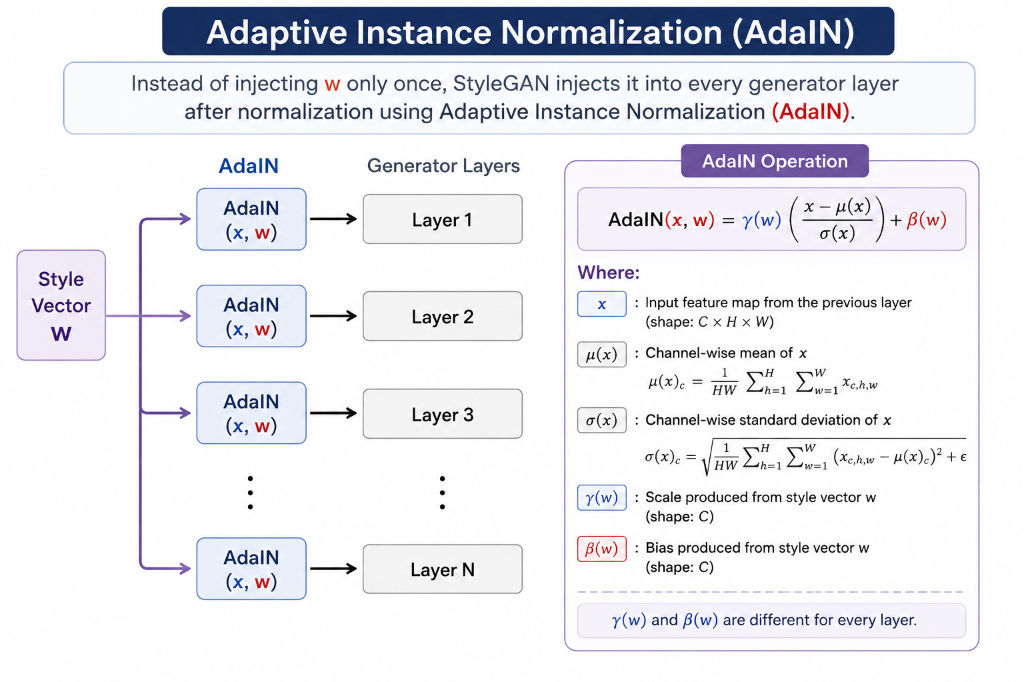
\includegraphics[width=0.88\textwidth]{figures/fig_9_8_adain_operation.png}
\caption{Adaptive Instance Normalization (AdaIN) Operation and Mathematical Formulation.}
\label{fig:adain_op}
\end{figure}

Different layers control different image properties:
\begin{itemize}
    \item \textbf{Early layers ($4\times4 - 8\times8$)}: Pose, face shape, coarse structure.
    \item \textbf{Middle layers ($16\times16 - 64\times64$)}: Eyes, nose, mouth, hairstyle.
    \item \textbf{Late layers ($128\times128 - 1024\times1024$)}: Skin texture, wrinkles, pores, fine details.
\end{itemize}

Instead of one global latent vector controlling everything, StyleGAN allows each layer to receive style independently.

\subsection*{Progressive Image Formation}

The image is generated from coarse to fine (e.g., the head first, then eyes/nose, and finally hair, skin texture, and tiny details):
\[
\text{Low Resolution} \longrightarrow \text{Overall Structure} \longrightarrow \text{Medium Resolution} \longrightarrow \text{Facial Features} \longrightarrow \text{High Resolution} \longrightarrow \text{Fine Details}
\]

\subsection*{III) Style Mixing \& Noise Injection}

\subsubsection*{Style Mixing}

Suppose we have two latent vectors:
\begin{itemize}
    \item $w_1 \rightarrow$ young woman
    \item $w_2 \rightarrow$ old man
\end{itemize}
Instead of using one style vector for every layer, we can combine them:
\begin{itemize}
    \item \textbf{Early layers}: $w_1$
    \item \textbf{Late layers}: $w_2$
\end{itemize}
$\Rightarrow \textbf{Result}$: Young face $+$ Old skin texture. Different parts of the Generator can receive different styles. This was impossible in earlier GANs.

\subsubsection*{Noise Injection}

Another innovation is per-layer random noise. StyleGAN adds small random noise inside each layer:
\[
\text{Feature Map} + \text{Noise} \longrightarrow \text{Next Layer}
\]
\begin{itemize}
    \item \textbf{Effect}: Very small stochastic details (freckles, skin pores, tiny hair strands, wrinkles).
    \item \textbf{$w$}: Controls the overall style.
    \item \textbf{Noise}: Controls tiny random variations.
\end{itemize}

\subsection*{IV) Learned Constant Tensor \& Generator Blocks}

Unlike previous GANs, the Generator does not start from $z$. Instead, it starts from a \textbf{Learned Constant Tensor} ($4\times4\times512$) that is learned during training and serves as the initial feature map.

\begin{figure}[H]
\centering
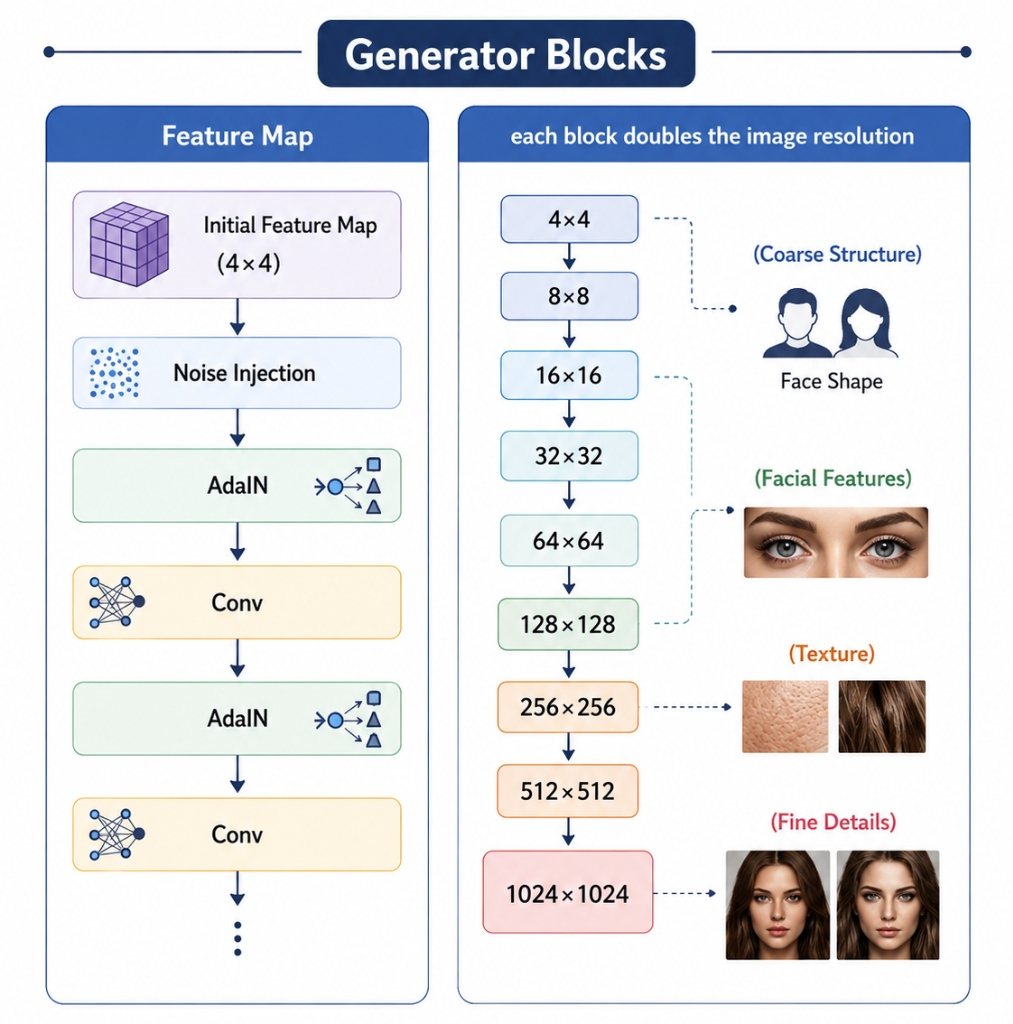
\includegraphics[width=0.88\textwidth]{figures/fig_9_9_stylegan_generator_blocks.png}
\caption{StyleGAN Generator Blocks and Multi-Scale Feature Resolution Control.}
\label{fig:stylegan_blocks}
\end{figure}

\begin{figure}[H]
\centering
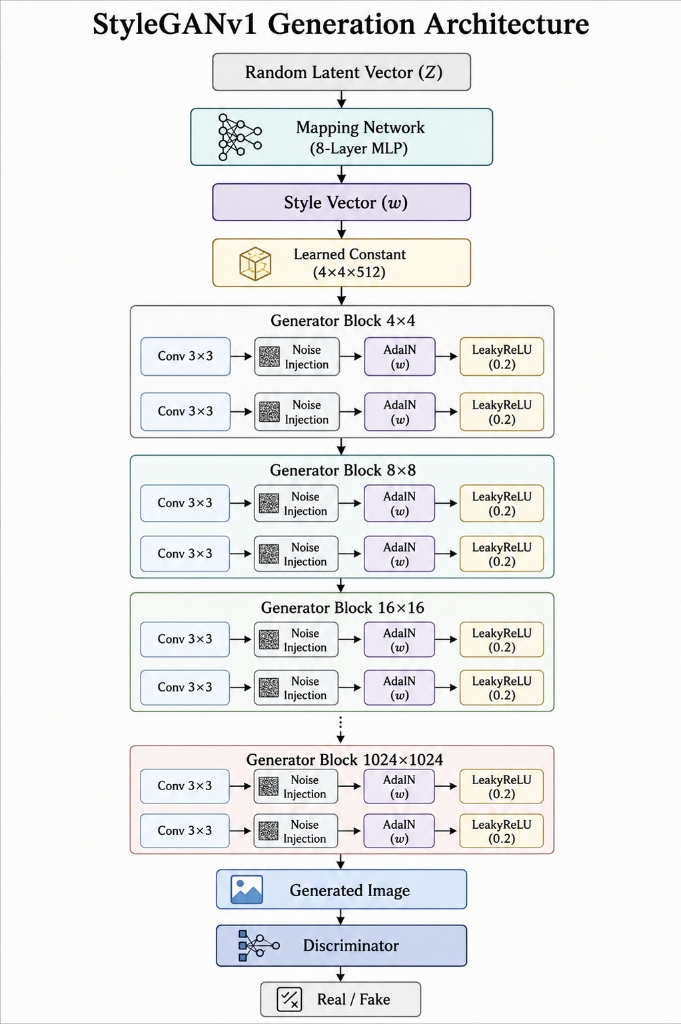
\includegraphics[width=0.88\textwidth]{figures/fig_9_10_stylegan_architecture.png}
\caption{Full StyleGANv1 Generation Pipeline and Discriminator Topology.}
\label{fig:stylegan_full}
\end{figure}

\subsection*{StyleGAN Advantages}

StyleGAN was revolutionary because for the first time, researchers could modify a generated face in a meaningful way (e.g., smile $\rightarrow$ increase, age $\rightarrow$ older, hair $\rightarrow$ longer, pose $\rightarrow$ rotate head) without changing everything else.

\begin{itemize}
    \item Disentangled latent space.
    \item Easy attribute manipulation.
    \item Different layers control different visual features.
    \item Highly realistic textures.
    \item Fine-grained control over generated images.
\end{itemize}

\section{WGAN (Wasserstein GAN) (2017)}

\begin{itemize}
    \item Original GAN suffers from vanishing gradients when the Discriminator becomes too strong.
    \item WGAN replaces the original loss function with the \textbf{Wasserstein (Earth Mover's) Distance}, providing a more useful learning signal.
\end{itemize}

\textbf{Main Idea}: Instead of classifying images as real or fake, WGAN measures how far the generated data distribution is from the real data distribution.
\begin{itemize}
    \item \textbf{Original GAN}: Discriminator $\rightarrow$ Probability ($0$ to $1$).
    \item \textbf{WGAN}: Critic $\rightarrow$ Real-valued score ($-\infty$ to $+\infty$).
\end{itemize}

The goal is to minimize the Wasserstein distance between the real and generated distributions:

\[
\begin{array}{ccc}
\textbf{Original GAN} & & \textbf{WGAN} \\
\text{Image} & & \text{Image} \\
\downarrow & & \downarrow \\
\text{Discriminator} & & \text{Critic} \\
\downarrow & & \downarrow \\
\text{Probability (Real/Fake)} & & \text{Real-valued Score}
\end{array}
\]

The architecture is almost the same as a GAN; the main differences are the loss function and replacing the Discriminator with a Critic.

WGAN improves GAN training by replacing the Discriminator with a Critic that outputs a real-valued score instead of a probability. It optimizes the Wasserstein (Earth Mover's) distance:
\[
W(P_r, P_g) = \inf_{\gamma \in \Pi(P_r, P_g)} \mathbb{E}_{(x,y) \sim \gamma}[\|x - y\|]
\]
Where $P_r$ is the real data distribution, $P_g$ is the generated data distribution, $\|x - y\|$ is the distance (cost) of moving one unit of mass from $x$ to $y$, and $\inf$ is the minimum over all possible transport plans.

This measures how far the generated data distribution is from the real data distribution, providing meaningful gradients throughout training even when generated images are initially poor. It results in more stable and reliable training with a much lower risk of vanishing gradients.

WGAN does not classify images (no Sigmoid $[0,1]$). Instead, the Critic assigns any real-valued score.

\begin{figure}[H]
\centering
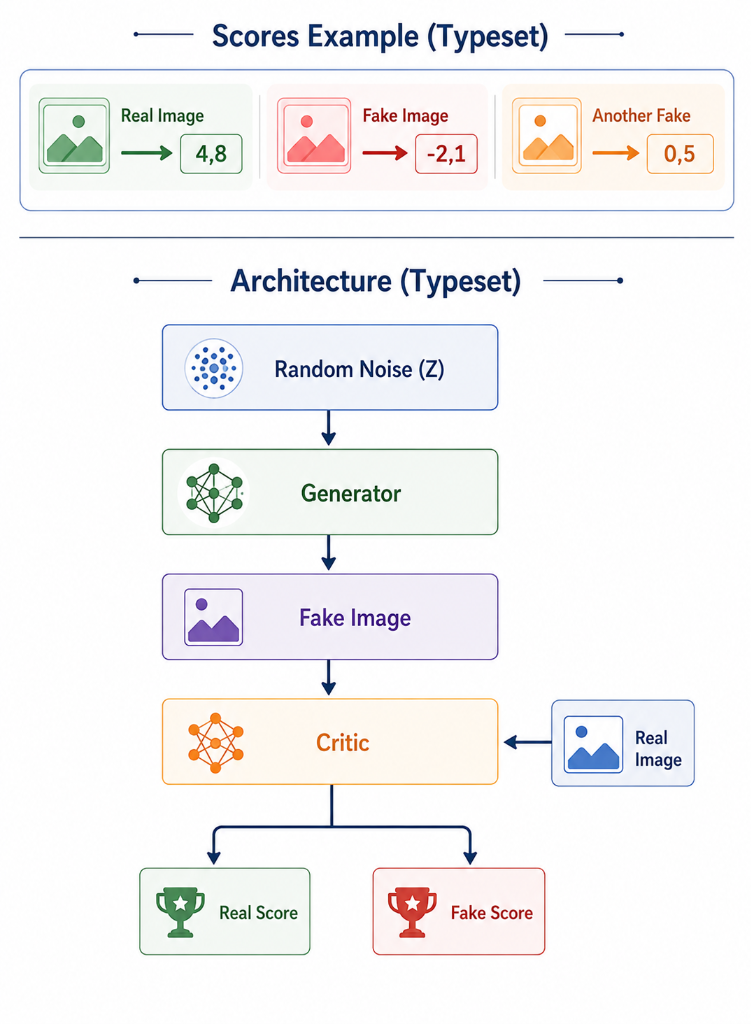
\includegraphics[width=0.88\textwidth]{figures/fig_9_6_wgan_architecture.png}
\caption{WGAN Critic Architecture and Scoring Mechanism.}
\label{fig:wgan_architecture}
\end{figure}

\subsection*{Weight Clipping}

After every update, the Critic's weights are forced into a small range e.g. $[-0.01, 0.01]$. This satisfies the requirement for the Wasserstein distance. However, clipping has drawbacks:
\begin{itemize}
    \item Reduces model capacity.
    \item Makes optimization harder.
    \item Can lead to poor performance.
\end{itemize}

\subsection*{WGAN-GP (Gradient Penalty)}

Researchers quickly improved WGAN by replacing weight clipping with a \textbf{Gradient Penalty (GP)}. Instead of forcing the weights to stay small, they directly penalize the gradients when they become too large.

\subsubsection*{Benefits}
\begin{itemize}
    \item More stable training.
    \item Better image quality.
    \item Easier optimization.
\end{itemize}

\subsubsection*{Limitations}
\begin{itemize}
    \item WGAN-GP is computationally more expensive because of the gradient penalty.
    \item It does not solve problems like controllability or image editing.
    \item It still inherits the complexity of adversarial training.
\end{itemize}

\section{BigGAN (2018)}

Researchers noticed an interesting trend:
\begin{itemize}
    \item As CNNs became larger $\longrightarrow$ performance improved.
    \item As Transformers became larger $\longrightarrow$ performance improved.
\end{itemize}
So they asked: what happens if we simply build a much bigger GAN? That idea led to BigGAN (2018).

Previous GANs were usually trained on CelebA, LSUN, or CIFAR-10. These datasets are relatively small. BigGAN was designed for ImageNet, which contains over 1 million images across 1000 object classes. Training a GAN on ImageNet was considered extremely difficult because the dataset is much larger, there are many object categories, and images are far more diverse.

\subsection*{Key Architectural \& Training Innovations in BigGAN}

\textbf{Main Idea}: BigGAN did not invent a completely new architecture; instead, it combined several good ideas:
\begin{itemize}
    \item Conditional GAN (control the class).
    \item Deeper and wider networks.
    \item Residual Blocks (ResNet).
    \item Large batch sizes.
    \item Spectral Normalization for stable training.
\end{itemize}
The philosophy was to scale everything up.

BigGAN demonstrated that scaling works. Simply making the models larger, training on more data, and using stable training techniques produced a huge leap in image quality. Generated images became sharper, more detailed, more diverse, and closer to real photographs.

\subsection*{Limitations of BigGAN}
\begin{itemize}
    \item Requires massive computational resources (often multiple high-end GPUs or TPUs).
    \item Training is expensive and time-consuming.
    \item Mainly designed for class-conditional image generation.
    \item Less flexible for image editing than StyleGAN.
\end{itemize}

\section{StyleGAN2 (2020) \& StyleGAN3 (2021)}

\subsection*{StyleGAN2 (2020)}

StyleGAN2 improved the original StyleGAN by removing visual artifacts (unwanted patterns or defects) and producing sharper, more realistic images. It redesigned parts of the Generator, leading to better image quality, smoother latent space interpolation, and more stable training. StyleGAN2 became the standard architecture for high-quality face generation.

\subsection*{StyleGAN3 (2021)}

StyleGAN3 focused on eliminating aliasing artifacts, making generated images more geometrically consistent. In StyleGAN2, small changes in the latent vector could cause textures (like hair or skin) to appear ``stuck'' to the image. StyleGAN3 solved this by making features move naturally with objects, producing more realistic animations and transformations.

\chapter{Diffusion Models}

By 2019, GANs had become incredibly powerful. Models like StyleGAN could generate faces so realistic that people often couldn't tell they were fake.
Researchers believed GANs might become the future of Image Generation. But despite their impressive results, one major problem remained: Training a GAN was still difficult.
Even after years of improvements (DCGAN, WGAN, StyleGAN, BigGAN...) GANs still suffered from several issues:
\begin{itemize}
    \item \textbf{Training instability} because the Generator and Discriminator constantly compete
    \item \textbf{Mode collapse}: where the Generator produces limited varieties of images
    \item \textbf{Sensitive hyperparameters}: making training difficult to reproduce
    \item \textbf{Balancing two networks is challenging}: if one becomes too strong, the other stops learning.
\end{itemize}

Researchers wanted a model that was:
\begin{itemize}
    \item easier to train
    \item more stable
    \item capable of producing diverse, high-quality images
\end{itemize}

Instead of asking: ``Can one network fool another network?'' \\
Researchers asked: ``Can we learn how to remove noise from an image?''

This question completely changed the direction of generative modeling. There would be:
\begin{itemize}
    \item no Generator vs Discriminator
    \item no adversarial game
    \item no competition
\end{itemize}
Instead, the model would learn a much simpler task: \textbf{Denoising}.

The brilliant idea behind diffusion models is to reverse the process of adding noise. Since gradually corrupting an image with Gaussian noise is simple and predictable, researchers realized that a neural network could be trained to learn the opposite process. Instead of generating an image directly, the model starts from pure random noise and removes a small amount of noise at each step, gradually reconstructing a realistic image. This transforms image generation into a sequence of simple denoising steps, making the learning process much more stable than the adversarial training used in GANs.

\subsection*{Why is This Easier Than GANs?}

Unlike GANs, where the Generator and Discriminator compete and the learning objective constantly changes, diffusion models train a single neural network with one fixed objective: predict and remove a small amount of noise. This stable objective makes diffusion models much easier to train.

\begin{itemize}
    \item Diffusion models do not learn to generate an image directly. Instead, they learn: \textbf{How To Remove a very small amount of Noise at each step.}
\end{itemize}

Diffusion models quickly became the dominant generative approach because they offered several advantages:
\begin{itemize}
    \item More stable training than GANs.
    \item Better diversity (less mode collapse).
    \item Excellent image quality.
    \item Easy to condition on text, segmentation maps, depth maps, or other inputs.
    \item Flexible enough for tasks like image editing, inpainting, and super-resolution.
\end{itemize}

\textbf{The main drawback} is that image generation is slower, since it requires many denoising steps.

\section{Core Principles of Diffusion}

Diffusion models were created to overcome the instability of GANs. Instead of training two competing networks, they train a single neural network to solve a simple and stable task: \textbf{Predict and Remove noise}.
\begin{itemize}
    \item \textbf{The Forward Process} gradually destroys an image by adding Gaussian noise until only random noise remains.
    \item \textbf{The Reverse Process} learns to remove that noise step by step, eventually reconstructing a realistic image. This simple idea became the foundation of modern image generation systems such as Stable Diffusion.
\end{itemize}

\subsection*{I) The Forward Diffusion Process}

The forward diffusion process gradually adds Gaussian noise to a clean image until it becomes pure random noise:
\begin{itemize}
    \item No neural network
    \item No learning
    \item Fixed corruption process
\end{itemize}

\textbf{Forward Process: starting from a clean image $x_0$:}
\[
x_0 \longrightarrow x_1 \longrightarrow x_2 \longrightarrow x_3 \longrightarrow x_4 \longrightarrow x_5 \dots \longrightarrow x_t
\]
Each step adds a small amount of Gaussian noise, making the image progressively noiser.

Adding all the noise at once would completely destroy the image and make it impossible to learn the reverse process.
By adding small amounts of noise at each step, the model only needs to learn how to reverse small changes, which is much easier.

\subsection*{Gaussian Noise}

The added noise is sampled from a standard Gaussian distribution:
\[
\epsilon \sim \mathcal{N}(0, 1)
\]
where:
\[
\text{Mean} = 0, \quad \text{Variance} = 1
\]
Each pixel receives a small random value sampled from this distribution. For example:
\[
\text{pixel} = 120, \quad \text{Noise} = +2 \quad \rightsquigarrow \quad \text{pixel} = 122
\]
or:
\[
\text{pixel} = 120, \quad \text{Noise} = -3 \quad \rightsquigarrow \quad \text{pixel} = 117
\]
Every pixel gets a different random value.

The forward process is a \textbf{Markov chain}. This means: each step depends only on the previous step, not on the entire history. For example:
\[
x_0 \longrightarrow x_1 \longrightarrow x_2 \longrightarrow x_3
\]
To compute $x_3$ we only need $x_2$; we do not need $x_0$ or $x_1$.

\subsection*{The Noise Schedule}

We don't add a random amount of noise each step. Instead, we define a noise schedule:
\begin{align*}
\text{step 1} &\longrightarrow 0.1\% \text{ noise} \\
\text{step 2} &\longrightarrow 0.2\% \text{ noise} \\
&\vdots \\
\text{step 1000} &\longrightarrow \text{Very noisy}
\end{align*}

The schedule controls how much noise is added at every step. Different schedules affect image quality and sampling speed.

After many diffusion steps, every image converges to the same distribution:
\[
x_T \sim \mathcal{N}(0, I)
\]
Regardless of whether the original image is a cat, car, house... it eventually becomes pure Gaussian noise.

Since every image eventually becomes Gaussian noise, generation becomes simple:
\begin{enumerate}
    \item Sample random noise $\sim \mathcal{N}(0, 1)$
    \item Learn how to reverse the diffusion
    \item Recover a realistic image
\end{enumerate}
Instead of learning to generate an image from scratch, the model only learns to remove noise little by little.

\subsection*{II) Reverse Diffusion}

After the forward process, the image becomes pure Gaussian noise $x_T$. The original image cannot be recovered directly because the information has been destroyed. Instead, the model must learn how to gradually remove the noise.

The reverse process performs the opposite of forward diffusion:
\[
\text{Pure noise} \longrightarrow \text{Less noise} \longrightarrow \text{Cleaner Image} \longrightarrow \dots \longrightarrow \text{Final Image}
\]
Instead of generating an image in one step, it is reconstructed progressively.

The diffusion model receives $(\text{Noisy Image}, \text{Time Step } t)$ and predicts: \textbf{Predicted Noise} ($\epsilon$). The network doesn't predict the clean image, it predicts the noise contained in the image.
Predicting the added Gaussian noise is simpler and more stable than predicting the clean image directly.

Once the noise is estimated:
\[
\text{Cleaner Image} = \text{Noisy Image} - \text{Predicted Noise}
\]
This process is repeated many times until a clean image is obtained.

\subsection*{Time Step Embedding}

The same noisy image may require different amounts of denoising depending on how much noise was originally added.
The time step $t$ tells the network:
\begin{itemize}
    \item how noisy the image is
    \item how much noise should be removed
\end{itemize}
Without $t$, the network would not know the current stage of the diffusion process.

\subsection*{Training Process}

For each training image:
\begin{enumerate}
    \item Start with a clean image $x_0$
    \item Randomly choose a time step $t$
    \item Add the corresponding Gaussian noise
    \item Feed $(\text{Noisy Image}, t)$ into the network
    \item Train the network to predict the true added noise using MSE Loss.
\end{enumerate}

\subsection*{Inference (Image Generation)}

During generation:
\begin{enumerate}
    \item Sample random Gaussian noise $x_T \sim \mathcal{N}(0, I)$
    \item Predict the noise
    \item Remove the predicted noise
    \item Repeat for all time steps until reaching $x_0$.
\end{enumerate}

\begin{figure}[H]
\centering
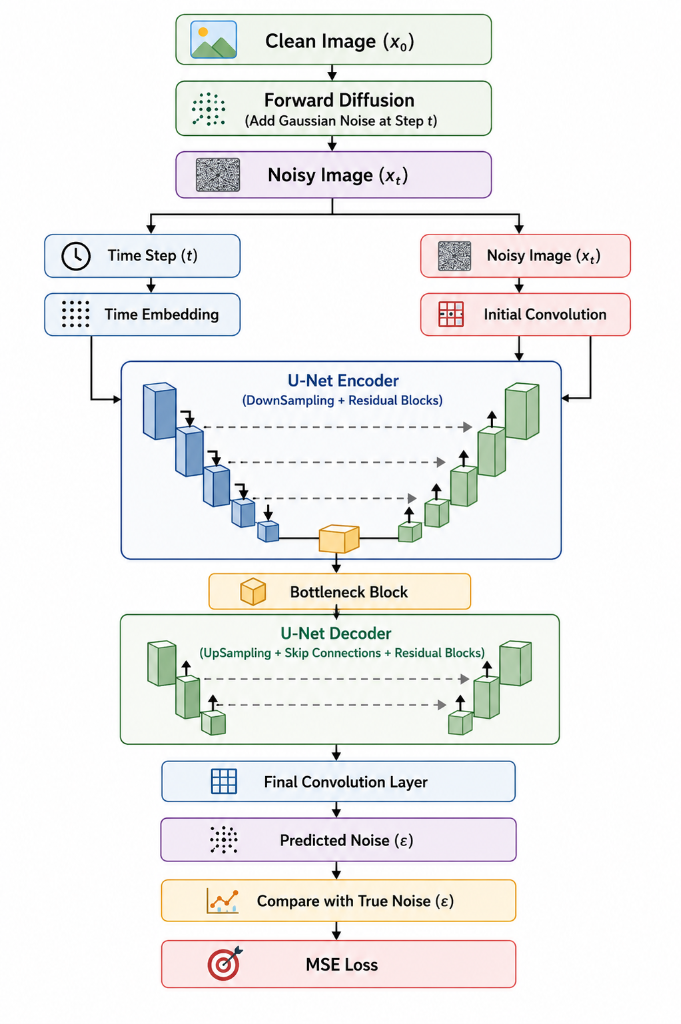
\includegraphics[width=0.88\textwidth]{figures/fig_10_1_diffusion_training_pipeline.png}
\caption{Diffusion Model Training and Noise Prediction Pipeline.}
\label{fig:diffusion_training_pipeline}
\end{figure}

\subsection*{Diffusion More Stable Than GANs}

\textbf{GAN:}
\begin{itemize}
    \item Two competing networks (Generator vs Discriminator)
    \item The objective changes during training
    \item Training can become unstable
\end{itemize}

\textbf{Diffusion:}
\begin{itemize}
    \item Only one neural network
    \item One fixed objective: predict the added noise
    \item Stable optimization using a simple MSE loss
\end{itemize}

\textbf{Summary:} The reverse diffusion process is the learned part of a diffusion model. Starting from pure Gaussian noise, a neural network repeatedly predicts the noise present in the current image and removes a small portion of it at each step. During training, the model receives a noisy image together with its time step and learns to predict the exact Gaussian noise that was added using an MSE loss. During inference, the same denoising process is applied iteratively to random noise until a realistic image is generated. Predicting noise instead of directly predicting the clean image is one of the key ideas that makes diffusion models stable and effective.

\section{DDPM (Denoising Diffusion Probabilistic Models)}

DDPM is the first practical diffusion model. It uses a U-Net to learn how to remove Gaussian noise from an image step by step until a clean image is reconstructed.
U-Net is well suited for this task because denoising is an image-to-image problem: the input is a noisy image and the output is a predicted noise map of the same size. Its encoder extracts high-level features, while the decoder reconstructs fine image details with the help of skip connections, enabling accurate denoising at every diffusion step.



\begin{figure}[H]
\centering
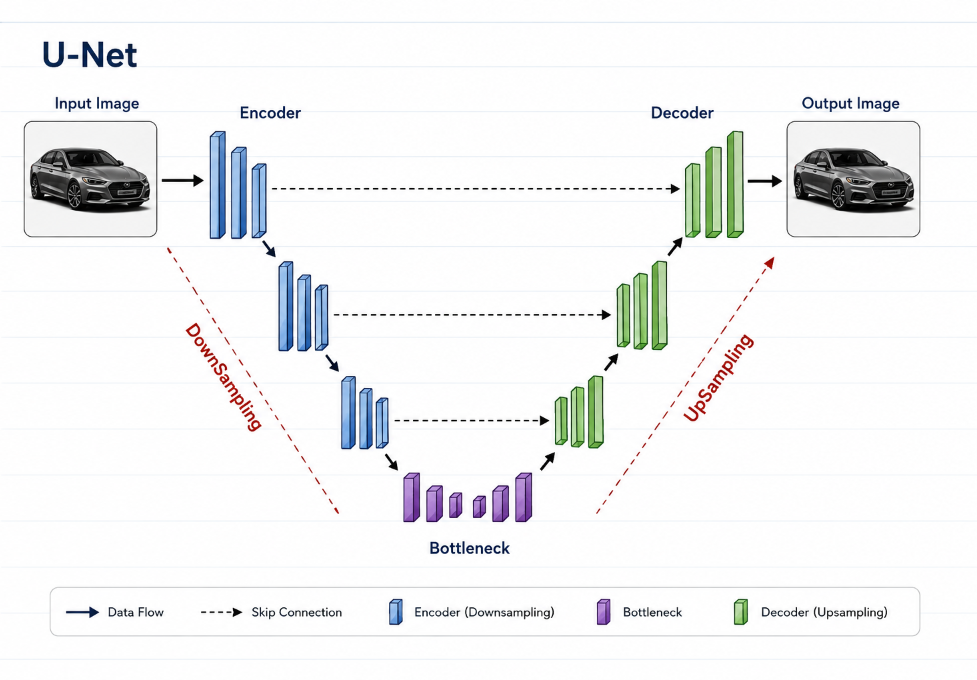
\includegraphics[width=0.88\textwidth]{figures/fig_10_2_unet_overview.png}
\caption{U-Net Architecture Overview for Image-to-Image Denoising.}
\label{fig:unet_overview}
\end{figure}

\begin{itemize}
    \item It was originally designed for image segmentation.
    \item Denoising is also an image-to-image problem.
\end{itemize}
Since both input and output are images of the same size, U-Net is an excellent choice.

\begin{figure}[H]
\centering
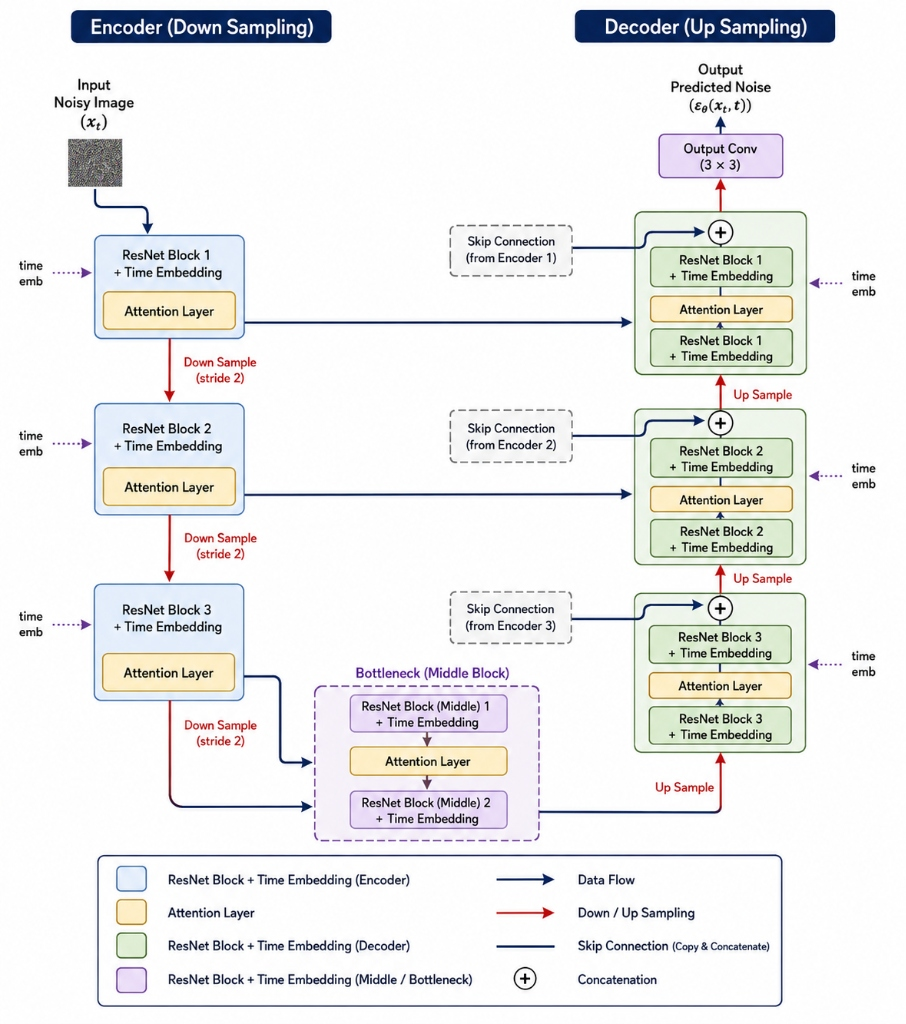
\includegraphics[width=0.95\textwidth]{figures/fig_10_3_ddpm_unet_detailed.jpg}
\caption{Detailed DDPM U-Net Architecture with ResNet Blocks, Attention Layers, and Time Embeddings.}
\label{fig:ddpm_unet_detailed}
\end{figure}

\begin{figure}[H]
\centering
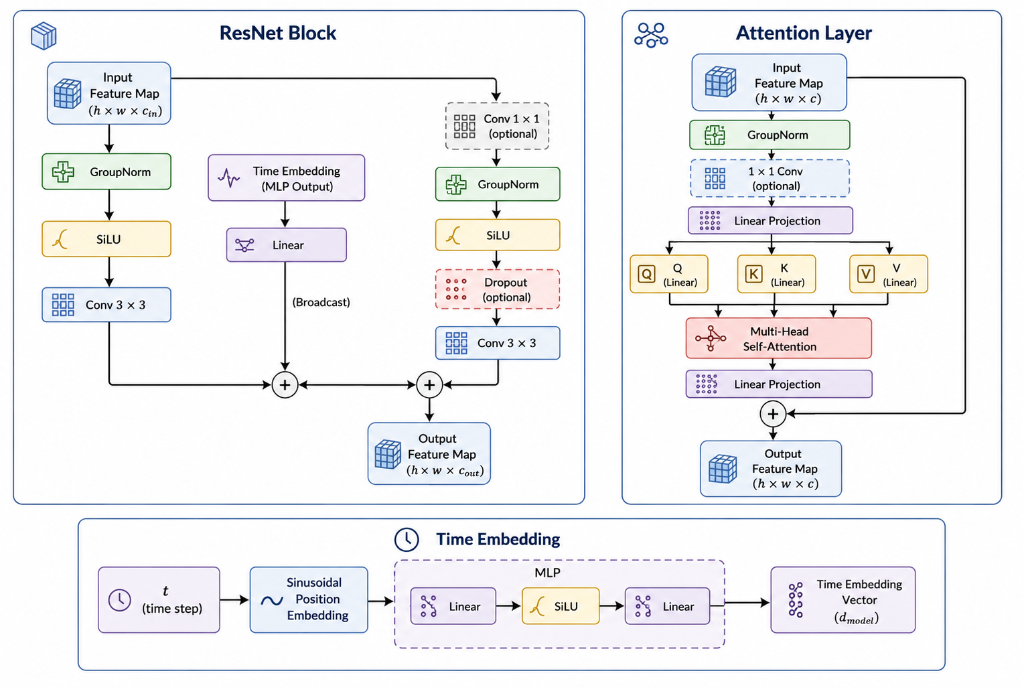
\includegraphics[width=0.95\textwidth]{figures/fig_10_4_unet_internal_components.png}
\caption{Internal Building Blocks of the DDPM U-Net: ResNet Block, Attention Layer, and Time Embedding MLP.}
\label{fig:unet_internal_components}
\end{figure}

\subsection*{Time Embedding Integration}

The U-Net receives two inputs:
\begin{itemize}
    \item Noisy image $x_t$
    \item Time step $t$
\end{itemize}

The integer $t$ is converted into a time embedding vector. This embedding is injected into multiple residual blocks so the network knows how much denoising to perform.

\subsection*{Training Process Step-by-Step}

\begin{enumerate}
    \item Select a clean image $x_0$
    \item Randomly choose a timestep $t$
    \item Add Gaussian noise to obtain $x_t$
    \item Feed $(x_t, t)$ into the U-Net
    \item Predict the added noise $\hat{\epsilon}$
    \item Compute the Loss $L_{\text{MSE}} = \|\epsilon - \hat{\epsilon}\|^2$
    \item Update the U-Net using backpropagation
\end{enumerate}

\begin{figure}[H]
\centering
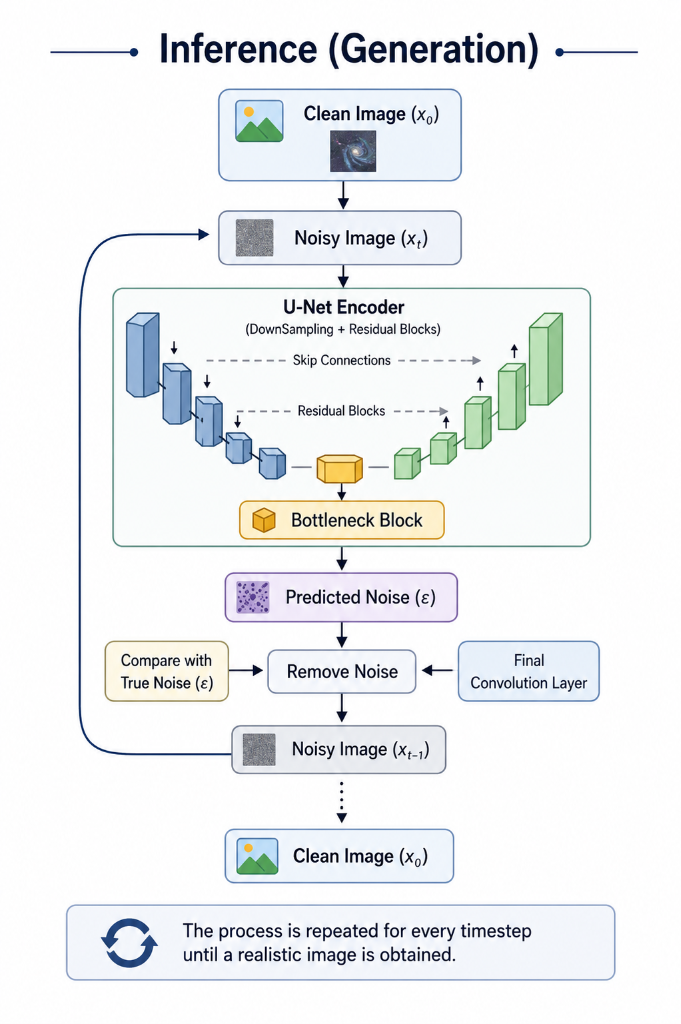
\includegraphics[width=0.88\textwidth]{figures/fig_10_5_diffusion_inference_pipeline.png}
\caption{Inference (Generation) Denoising Loop in Diffusion Models.}
\label{fig:diffusion_inference_pipeline}
\end{figure}

\section{Classifier-Free Guidance (CFG)}

\subsection*{I) Guidance}

Without additional information, diffusion models generate random images. To generate a specific object or scene, the model needs guidance.

\textbf{The Main Idea of Classifier Guidance is using two models:}
\begin{itemize}
    \item Diffusion model
    \item External image classifier
\end{itemize}
The classifier provides gradients that push the generated image toward the desired class.

\textbf{Limitation:}
\begin{itemize}
    \item Requires training an additional classifier
    \item More computationally expensive
\end{itemize}

\subsection*{II) Classifier-Free Guidance (CFG)}

Instead of using an external classifier, the diffusion model learns both:
\begin{itemize}
    \item \textbf{Conditional Generation}: Noise + Prompt
    \item \textbf{Unconditional Generation}: Noise only
\end{itemize}

During training, the conditioning information (text/class) is randomly removed, allowing one model to learn both behaviors.

\subsection*{CFG During Inference}

During inference, the model performs two noise predictions:
\begin{enumerate}
    \item \textbf{Unconditional prediction}: Noise only ($\hat{\epsilon}_{\text{uncond}}$)
    \item \textbf{Conditional prediction}: Noise + Prompt ($\hat{\epsilon}_{\text{cond}}$)
\end{enumerate}
They are combined using:
\[
\hat{\epsilon}_{\text{CFG}} = \hat{\epsilon}_{\text{uncond}} + w \cdot (\hat{\epsilon}_{\text{cond}} - \hat{\epsilon}_{\text{uncond}})
\]
where $w = \text{Guidance Scale}$: Controls how strongly the prompt influences the generated image.
\begin{itemize}
    \item \textbf{Low scale}: More creative, weaker adherence to the prompt
    \item \textbf{High scale}: Follows the prompt more closely
\end{itemize}
Typically values for CFG scale are $7 - 8$.

Today, almost every text-to-image diffusion model uses Classifier-Free Guidance.
Examples:
\begin{itemize}
    \item Stable Diffusion
    \item SDXL
    \item FLUX
    \item Many modern diffusion models
\end{itemize}
because it:
\begin{itemize}
    \item requires no extra classifier
    \item is simple
    \item gives users control over prompt strength.
\end{itemize}

\begin{figure}[H]
\centering
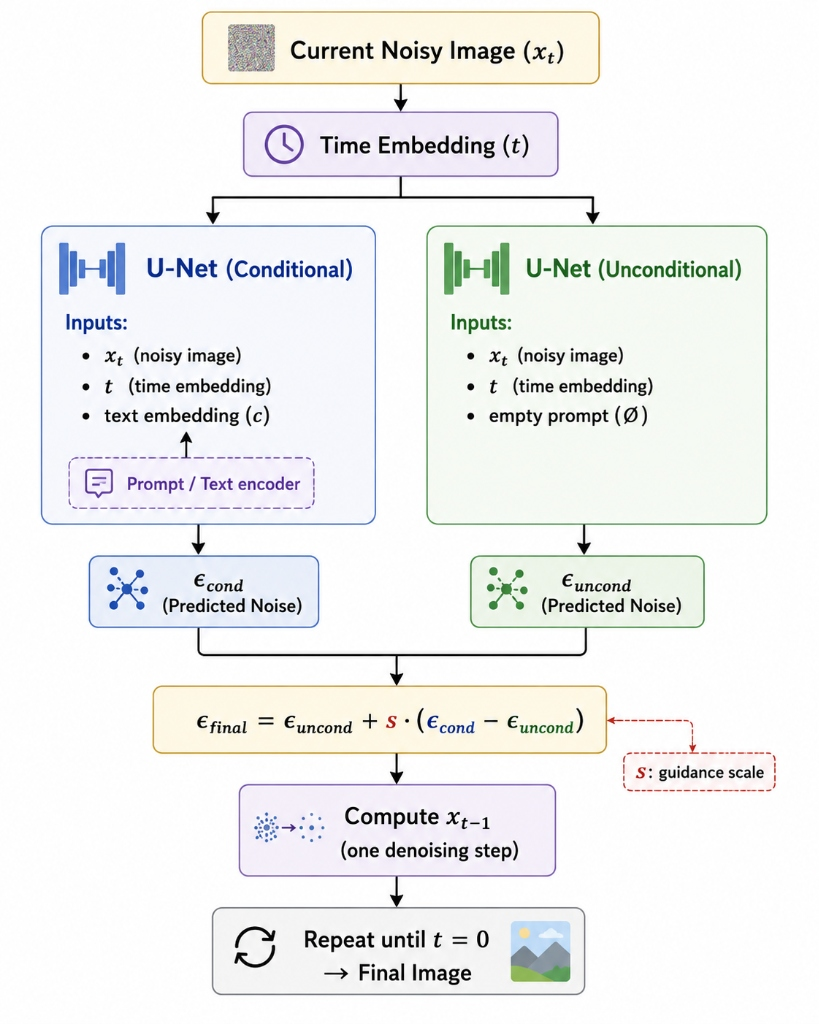
\includegraphics[width=0.88\textwidth]{figures/fig_10_6_classifier_free_guidance.jpg}
\caption{Classifier-Free Guidance (CFG) Denoising Pipeline.}
\label{fig:classifier_free_guidance}
\end{figure}

\section{Latent Diffusion Models (LDM)}

DDPM and DDIM perform diffusion directly on pixels.
For example, suppose we have a $512 \times 512$ RGB image:
\[
512 \times 512 \times 3 \longrightarrow 786,432 \text{ values}
\]
At every denoising step, the U-Net processes all 786,432 pixel values. For 1,000 denoising steps, this requires an enormous amount of computation and memory.
Researchers asked: ``Do we really need to diffuse millions of pixels?''

The main idea of LDM is to use a Variational Autoencoder (VAE) to compress an image into a much smaller latent representation before diffusion.
The diffusion model never operates on the original image; it works entirely in the latent space.

\begin{figure}[H]
\centering
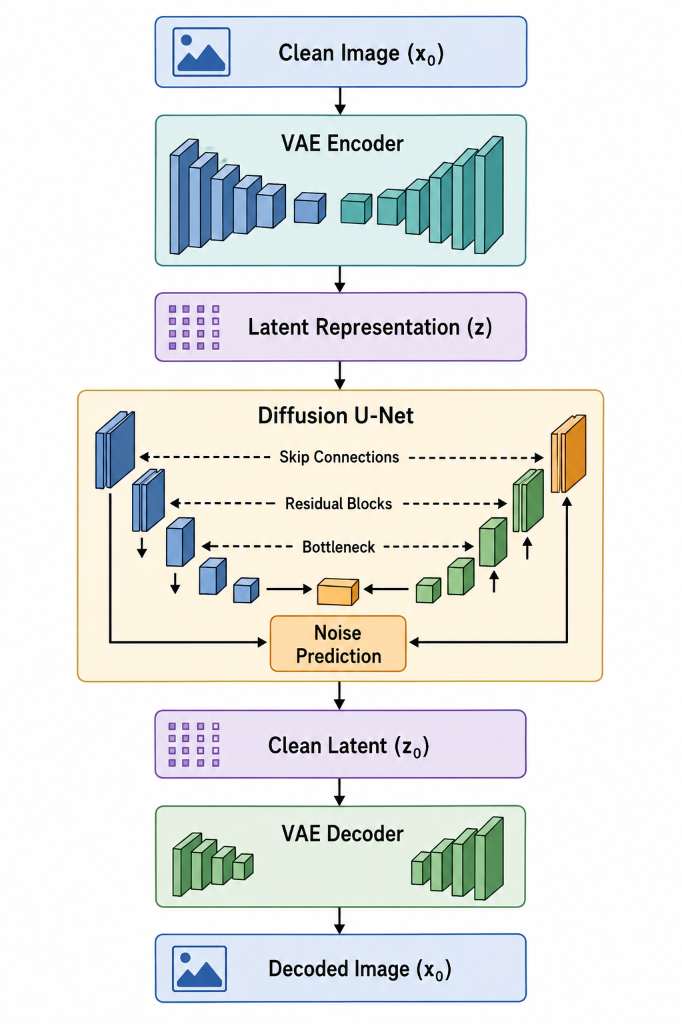
\includegraphics[width=0.75\textwidth]{figures/fig_10_7_latent_diffusion_architecture.png}
\caption{Latent Diffusion Model Architecture.}
\label{fig:latent_diffusion_architecture}
\end{figure}

LDM models are much faster because the latent diffusion process is performed on a compressed representation instead of raw pixels.
The VAE encoder compresses a high-resolution image into a much smaller representation, reducing the amount of data processed by the U-Net at every denoising step.

For example, a $512 \times 512 \times 3$ image ($786,432$ values) is compressed into a $64 \times 64 \times 4$ latent representation ($16,384$ values), meaning the model processes about $48\times$ fewer values.
This drastically reduces both computational cost and memory usage while maintaining high image quality, making image generation dramatically faster.

The VAE compresses the image while preserving key semantic information (objects, colors, textures) and removing unnecessary details (such as exact pixel noise). This allows the diffusion model to focus on high-level image generation instead of low-level pixel noise.

\begin{figure}[H]
\centering
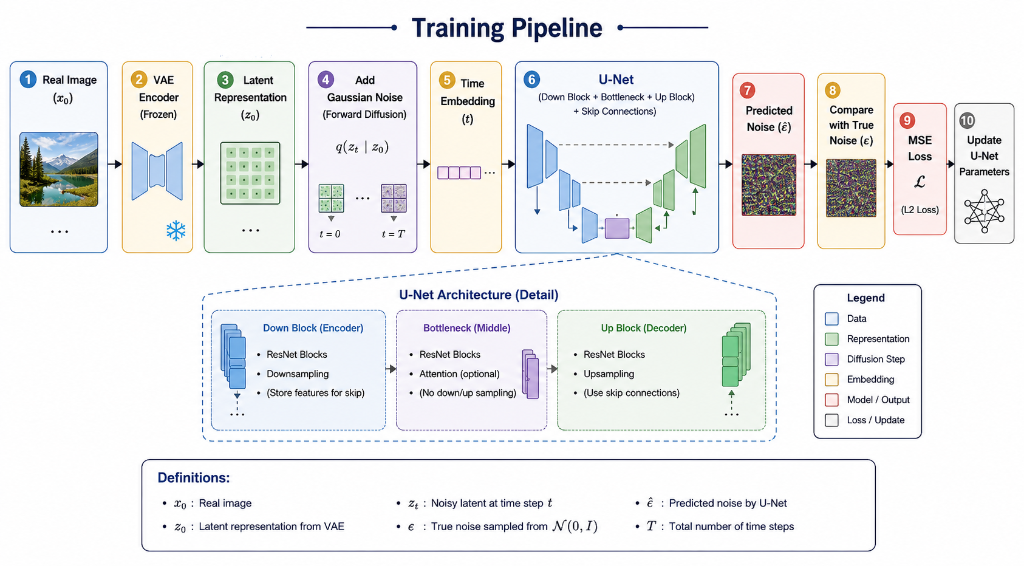
\includegraphics[width=0.95\textwidth]{figures/fig_10_8_ldm_training_pipeline.png}
\caption{Training Pipeline for Latent Diffusion Models.}
\label{fig:ldm_training_pipeline}
\end{figure}

\begin{figure}[H]
\centering
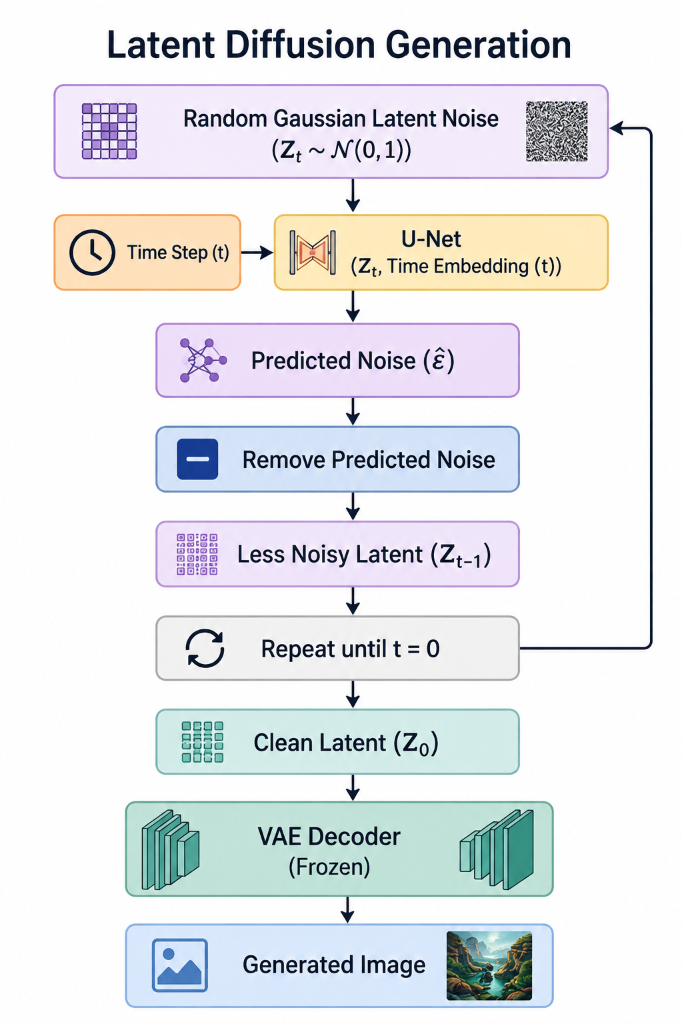
\includegraphics[width=0.75\textwidth]{figures/fig_10_9_ldm_generation_pipeline.png}
\caption{Latent Diffusion Generation and Inference Pipeline.}
\label{fig:ldm_generation_pipeline}
\end{figure}

\subsection*{Advantages of LDM}
\begin{itemize}
    \item Uses much less GPU memory
    \item Faster training and generation
    \item Supports high-resolution image generation
    \item Maintains excellent image quality
\end{itemize}

\subsection*{Drawbacks}
\begin{itemize}
    \item Image quality depends on the VAE compression quality (if information is lost during compression, it cannot be recovered)
    \item The system requires two models: VAE and Diffusion Model.
\end{itemize}

\section{Stable Diffusion}

Stable Diffusion is a Latent Diffusion Model (LDM) that can generate images directly from text prompts.
It combines:
\begin{itemize}
    \item \textbf{VAE}: Compresses and reconstructs images
    \item \textbf{Diffusion Model (U-Net)}: Denoises the latent representation
    \item \textbf{CLIP Text Encoder}: Converts text prompts into numerical text embeddings that the diffusion model can understand
    \item \textbf{Cross-Attention}: Connects the text embeddings with the image generation process
    \item \textbf{CFG (Classifier-Free Guidance)}: Controls how strongly the generated image follows the prompt.
\end{itemize}

\begin{figure}[H]
\centering
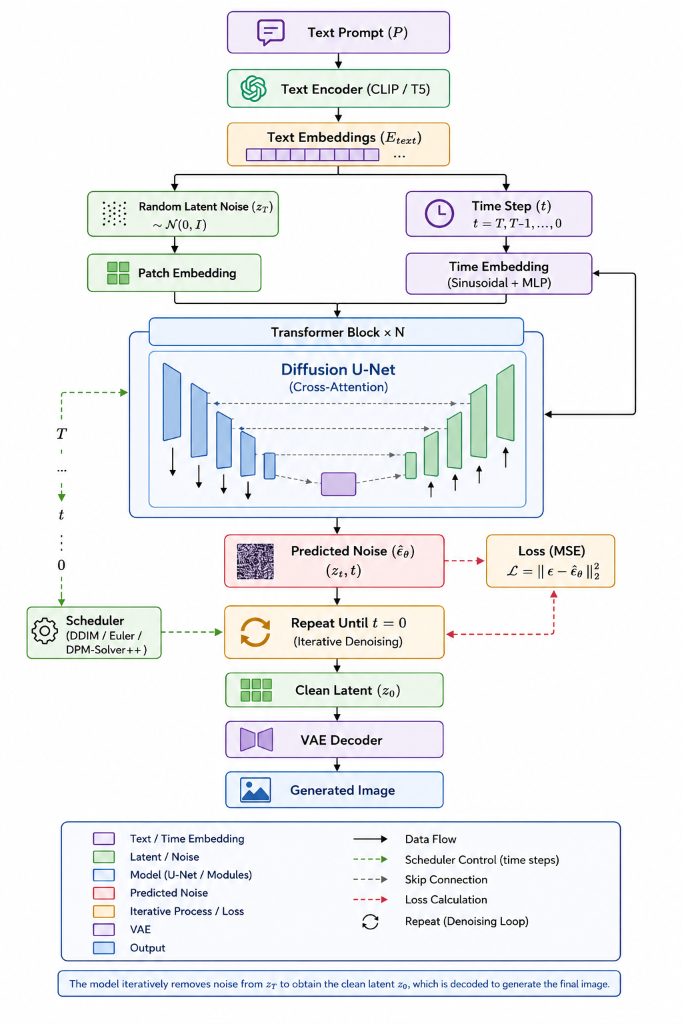
\includegraphics[width=0.95\textwidth]{figures/fig_10_10_conditioning_mechanisms.png}
\caption{Conditioning Mechanisms in Latent Diffusion Models.}
\label{fig:conditioning_mechanisms}
\end{figure}

In the standard classifier-free guidance (CFG) mechanism, the denoiser performs two noise predictions at each denoising step:

\begin{enumerate}
    \item A prediction without the text prompt (unconditional prediction).
    \item A prediction conditioned on the text prompt (conditional prediction).
\end{enumerate}

These two predictions are combined using \textbf{Classifier-Free Guidance (CFG)} to produce the final noise estimate for that denoising step. Other diffusion systems may use different conditioning or guidance mechanisms.

Stable Diffusion became extremely popular and revolutionary because it:

\begin{itemize}
    \item Generates high-quality images.
    \item Runs efficiently on consumer GPUs.
    \item Supports text-to-image generation.
    \item Uses Classifier-Free Guidance (CFG) to improve prompt adherence.
    \item Can be fine-tuned on new styles and concepts (e.g., LoRA and ControlNet).
    \item Has a large open-source ecosystem of models, tools, and extensions.
\end{itemize}

\section{Diffusion Transformers (DiT)}

Diffusion Transformers are a family of diffusion-model architectures that use a Vision Transformer (ViT)-style backbone instead of a U-Net.
The noisy latent is split into patches, converted into tokens, and processed with Transformer blocks to predict the noise.

DiT changes the denoising backbone; its latent representation, conditioning, guidance, and training design depend on the specific diffusion system.

\subsection*{Why Replace U-Net?}
\begin{itemize}
    \item U-Net relies on Convolutions, which mainly focus on local features.
    \item Transformers use Self-Attention, allowing every patch to interact with every other patch.
    \item Transformers scale much better as dataset size, compute, and model parameters increase.
\end{itemize}

\begin{figure}[H]
\centering
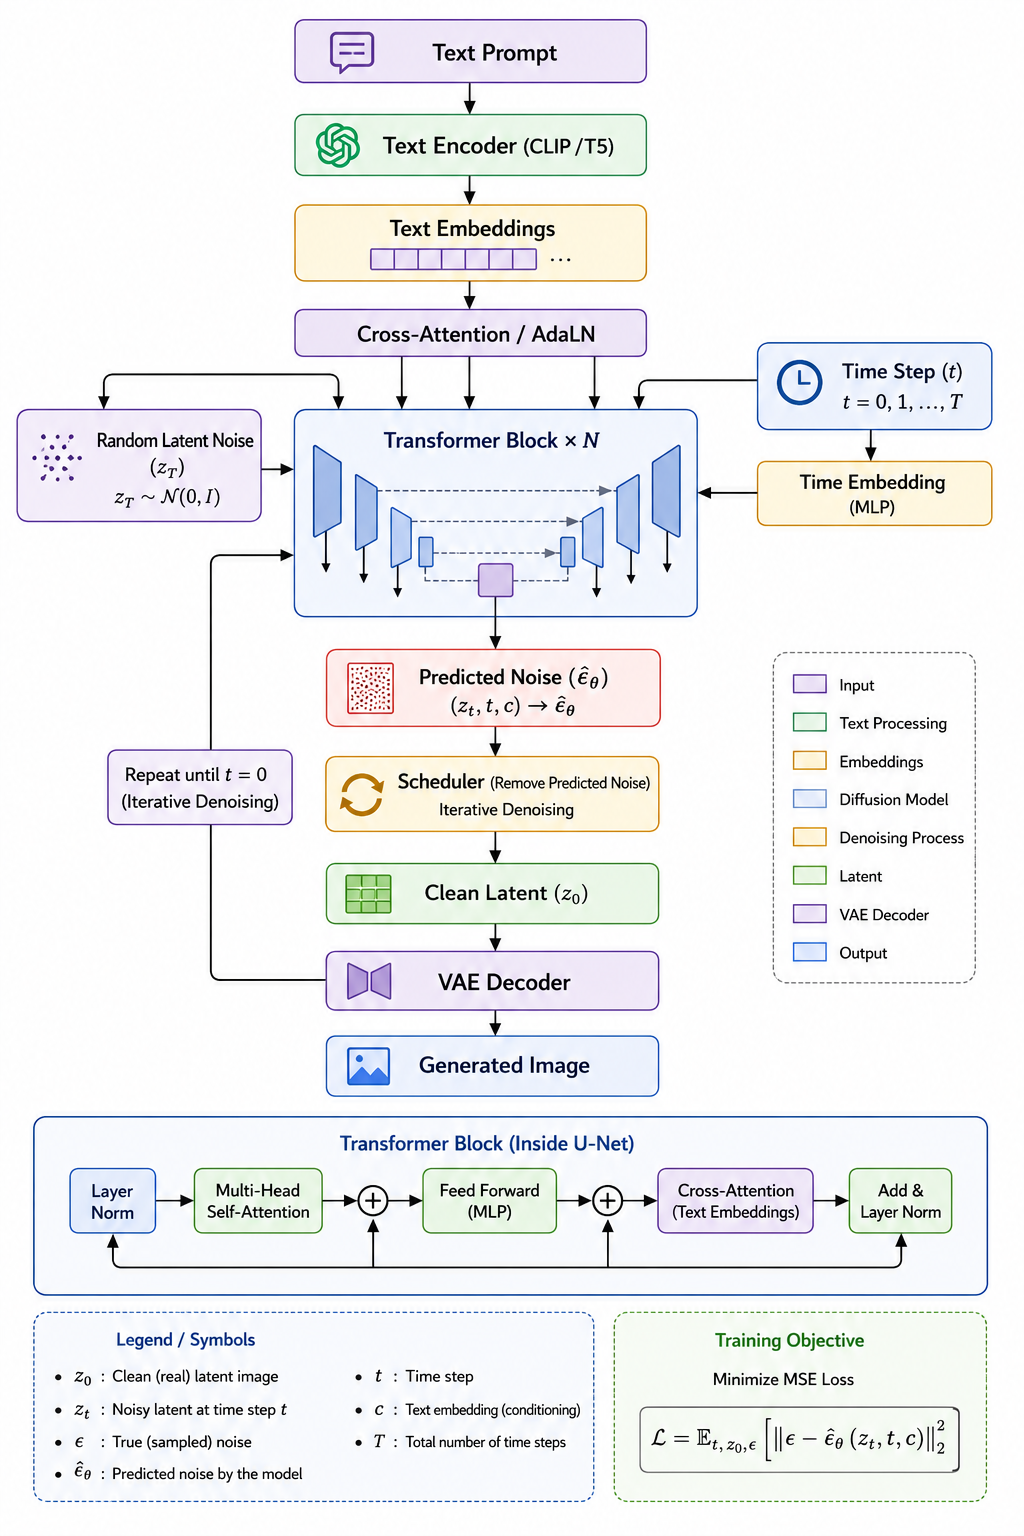
\includegraphics[width=0.95\textwidth]{figures/ChatGPT Image Aug 5, 2026, 03_19_00 AM.png}
\caption{Diffusion Transformer (DiT) Architecture Details.}
\label{fig:dit_architecture}
\end{figure}

\section{DiT Conditioning and Adaptive Layer Normalization}

A Diffusion Transformer (DiT) uses a Vision Transformer (ViT)-style architecture as its denoising backbone. In the original DiT design, the noisy latent produced by the VAE is divided into small patches, which are converted into latent patch tokens and processed by a stack of Transformer blocks.

Unlike a standard Vision Transformer, DiT must also receive the conditioning information required by the diffusion process. Each Transformer block therefore combines three sources of information:

\begin{enumerate}
    \item \textbf{Latent patch tokens}, obtained from the noisy latent representation.
    \item \textbf{Time embedding}, which indicates the current diffusion step $t$, allowing the model to know where it is in the denoising process.
    \item \textbf{Text embedding}, generated by a text encoder from the input prompt, providing semantic guidance for image generation.
\end{enumerate}

Rather than injecting the time and text embeddings through convolutional blocks as in U-Net-based diffusion models, DiT incorporates this conditioning information into every Transformer block using \textbf{Adaptive Layer Normalization (AdaLN)}:

\[
\text{AdaLN}(x,t,c)=\gamma(t,c)\,\text{LN}(x)+\beta(t,c),
\]

where $x$ represents the Transformer token features, $\text{LN}(\cdot)$ denotes Layer Normalization, and $\gamma(t,c)$ and $\beta(t,c)$ are learned scale and shift parameters generated from the time-step and text-conditioning embeddings. Consequently, every Transformer block is aware of both the current diffusion step and the prompt being followed, enabling the model to adapt its feature activations throughout the denoising process.

By leveraging global self-attention and the excellent scaling properties of Transformers, DiT has become one of the leading architectures for modern diffusion models. As the model size, training dataset, and computational resources increase, its image generation quality continues to improve, making Transformer-based diffusion models highly scalable.

\section{SDXL (Stable Diffusion XL)}

SDXL is an improved version of Stable Diffusion that significantly increases model capacity while preserving the original latent diffusion framework. Rather than introducing a completely new architecture, SDXL retains the same fundamental components, including the Variational Autoencoder (VAE), latent diffusion process, U-Net denoiser, and Classifier-Free Guidance (CFG), while incorporating several important enhancements.

The main improvements of SDXL include:

\begin{itemize}
    \item A larger and more expressive U-Net architecture.
    \item Dual text encoders (CLIP ViT-L and OpenCLIP ViT-bigG), enabling richer prompt understanding.
    \item Improved image quality and native high-resolution image generation at $1024 \times 1024$ pixels.
\end{itemize}
\section{FLUX}

FLUX (2024) is a modern text-to-image model developed by Black Forest Labs.
Instead of the traditional U-Net, FLUX uses a Transformer-based backbone (similar in spirit to DiT).

Key improvements:
\begin{itemize}
    \item Better prompt adherence
    \item Better typography (rendering text inside images)
    \item Better human anatomy (hands, faces)
    \item Better overall image quality.
\end{itemize}
FLUX is currently one of the strongest open-weights image generation models.

\section{Flow Matching}

Flow Matching is one of the newest directions in generative modeling.
Instead of predicting noise at each step, the model predicts a velocity vector field (direction and speed) that continuously transforms random noise into a real image.

Flow Matching generates images by learning the direction (velocity) that continuously transforms random noise into a real image, rather than learning how to remove noise at each step.

\begin{figure}[H]
\centering
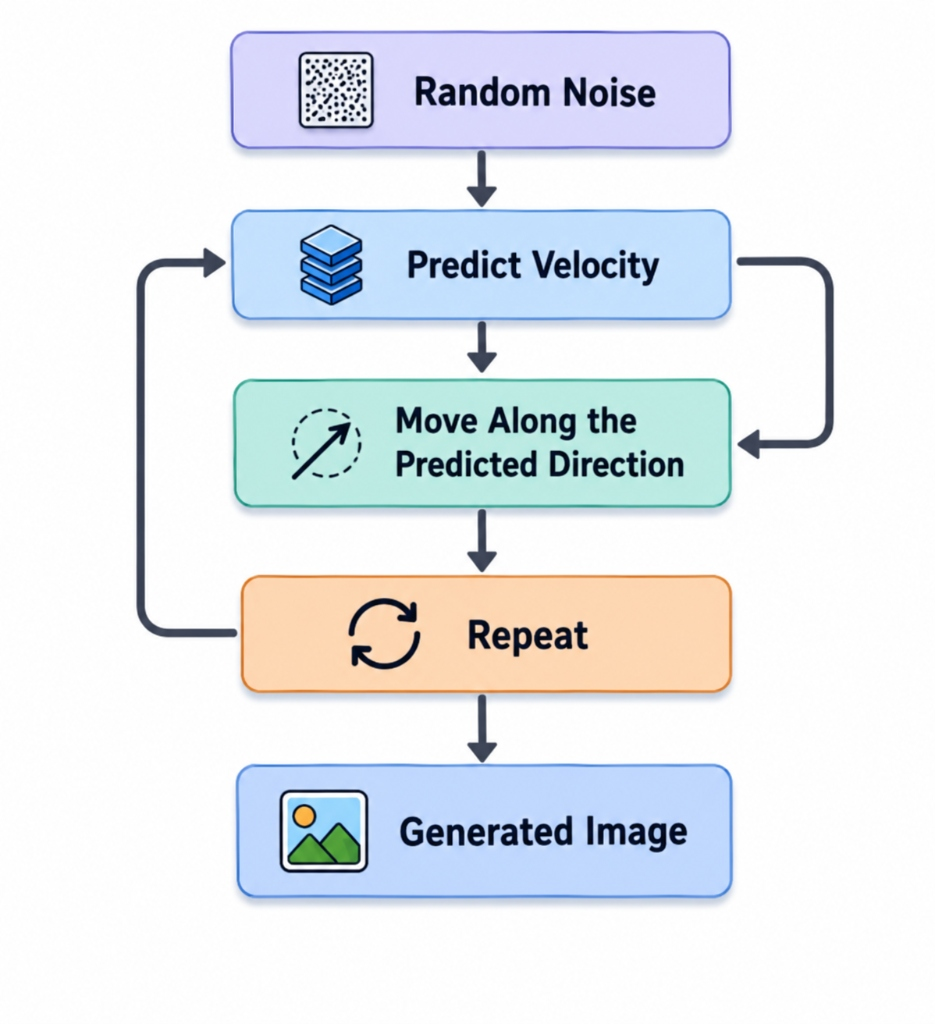
\includegraphics[width=0.65\textwidth]{figures/fig_10_12_flow_matching.jpg}
\caption{Flow Matching Denoising Loop.}
\label{fig:flow_matching}
\end{figure}

\subsection*{Advantages}
\begin{itemize}
    \item Simpler training objective
    \item Faster image generation with efficient ODE solvers
    \item Uses almost the same architecture as modern diffusion models
    \item Achieves state-of-the-art image generation quality.
\end{itemize}

\chapter{Meta-Learning}

\section{Introduction to Meta-Learning}

Traditional deep learning is designed to solve a single fixed task. A model is trained on a large labeled dataset containing predefined classes such as \textit{Dog}, \textit{Cat}, \textit{Bird}, and \textit{Horse}. During training, the model learns to recognize only these classes.

\begin{figure}[H]
\centering
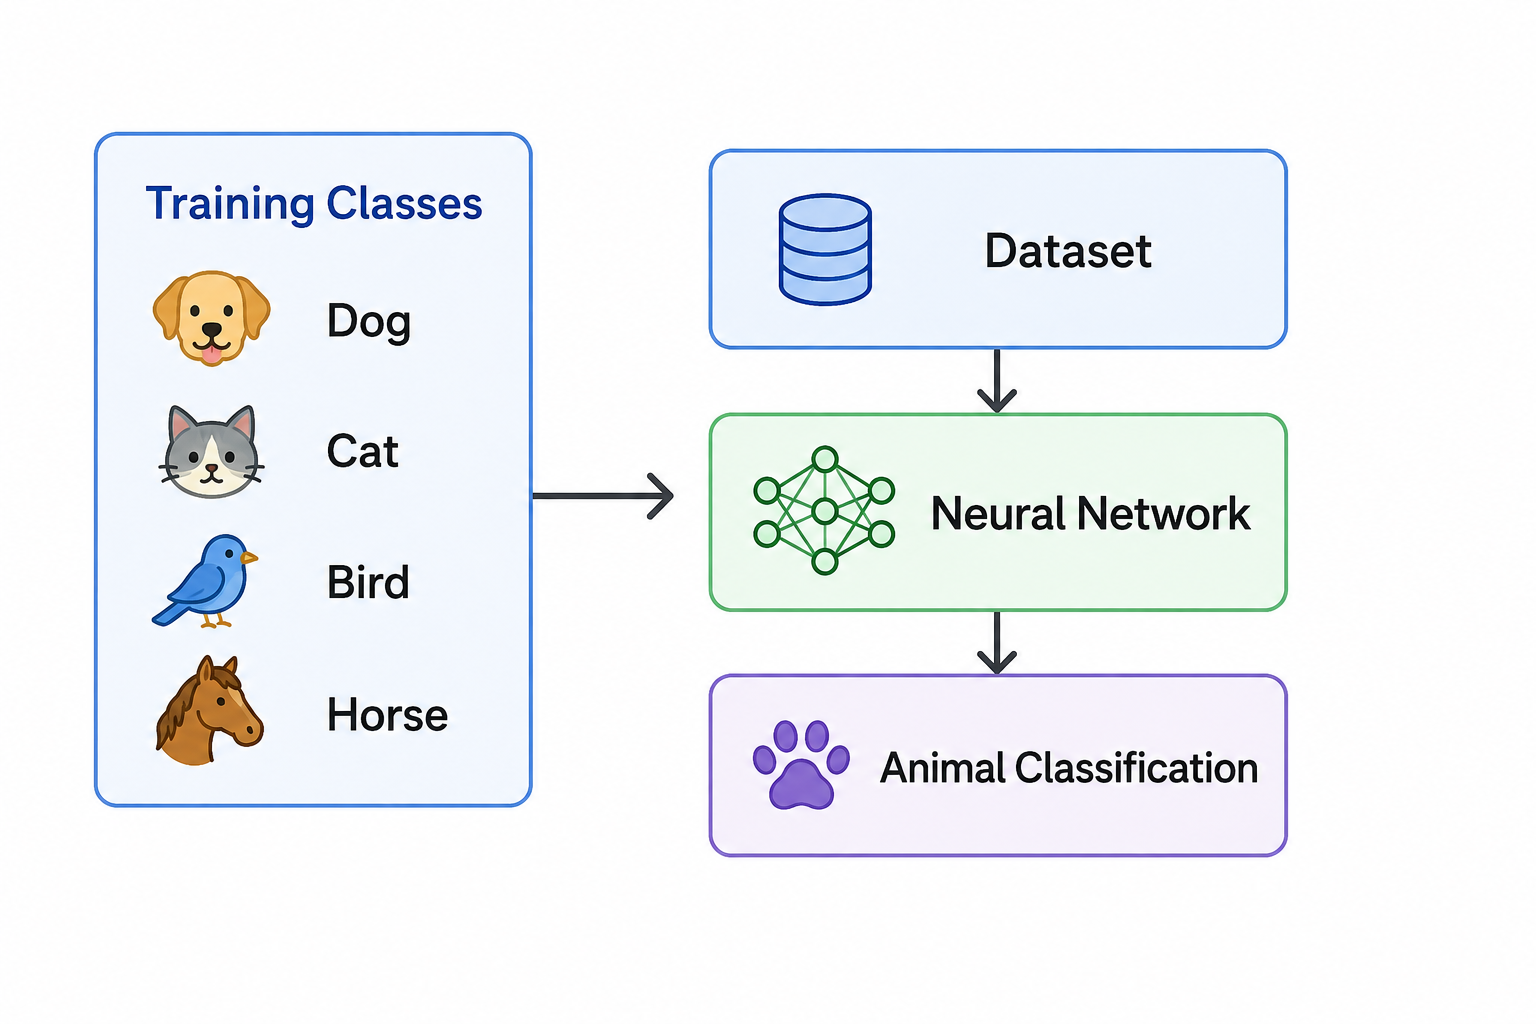
\includegraphics[width=0.85\textwidth]{figures/11-1 figure.png}
\label{fig:traditional_supervised_learning}
\end{figure}

After training, the model performs well on these known classes. However, when a new task introduces previously unseen classes, such as \textit{Camel} or \textit{Koala}, the model cannot recognize them effectively because it has never encountered these categories during training.

To adapt the model to the new task, it is typically necessary to:

\begin{itemize}
    \item Collect a large number of labeled examples for the new classes.
    \item Fine-tune or retrain the model using the new dataset.
    \item Repeat the training process whenever a new task is introduced.
\end{itemize}

Therefore, traditional deep learning is highly effective for solving a single predefined task, but it adapts slowly to new tasks or new classes because it requires substantial labeled data and additional training.

\subsection*{Can a Model Learn a New Task from 1 or 5 Examples?}

Humans can learn a new concept from seeing just one or two examples. They do not require thousands of observations. In contrast, traditional deep learning requires a fixed mapping from input to output, so the model cannot perform on a new task without acquiring labeled data and retraining or fine-tuning before it can perform.

\textbf{The Main Idea of Meta-Learning}:
Meta-Learning focuses on training across many tasks to learn how to quickly adapt to new tasks. Instead of optimizing the model for a single problem, it trains the model on many tasks so that it acquires a general learning strategy that can be used when encountering unseen tasks.

This is why Meta-Learning is called: \textbf{``Learning to Learn''}.

\begin{figure}[H]
\centering
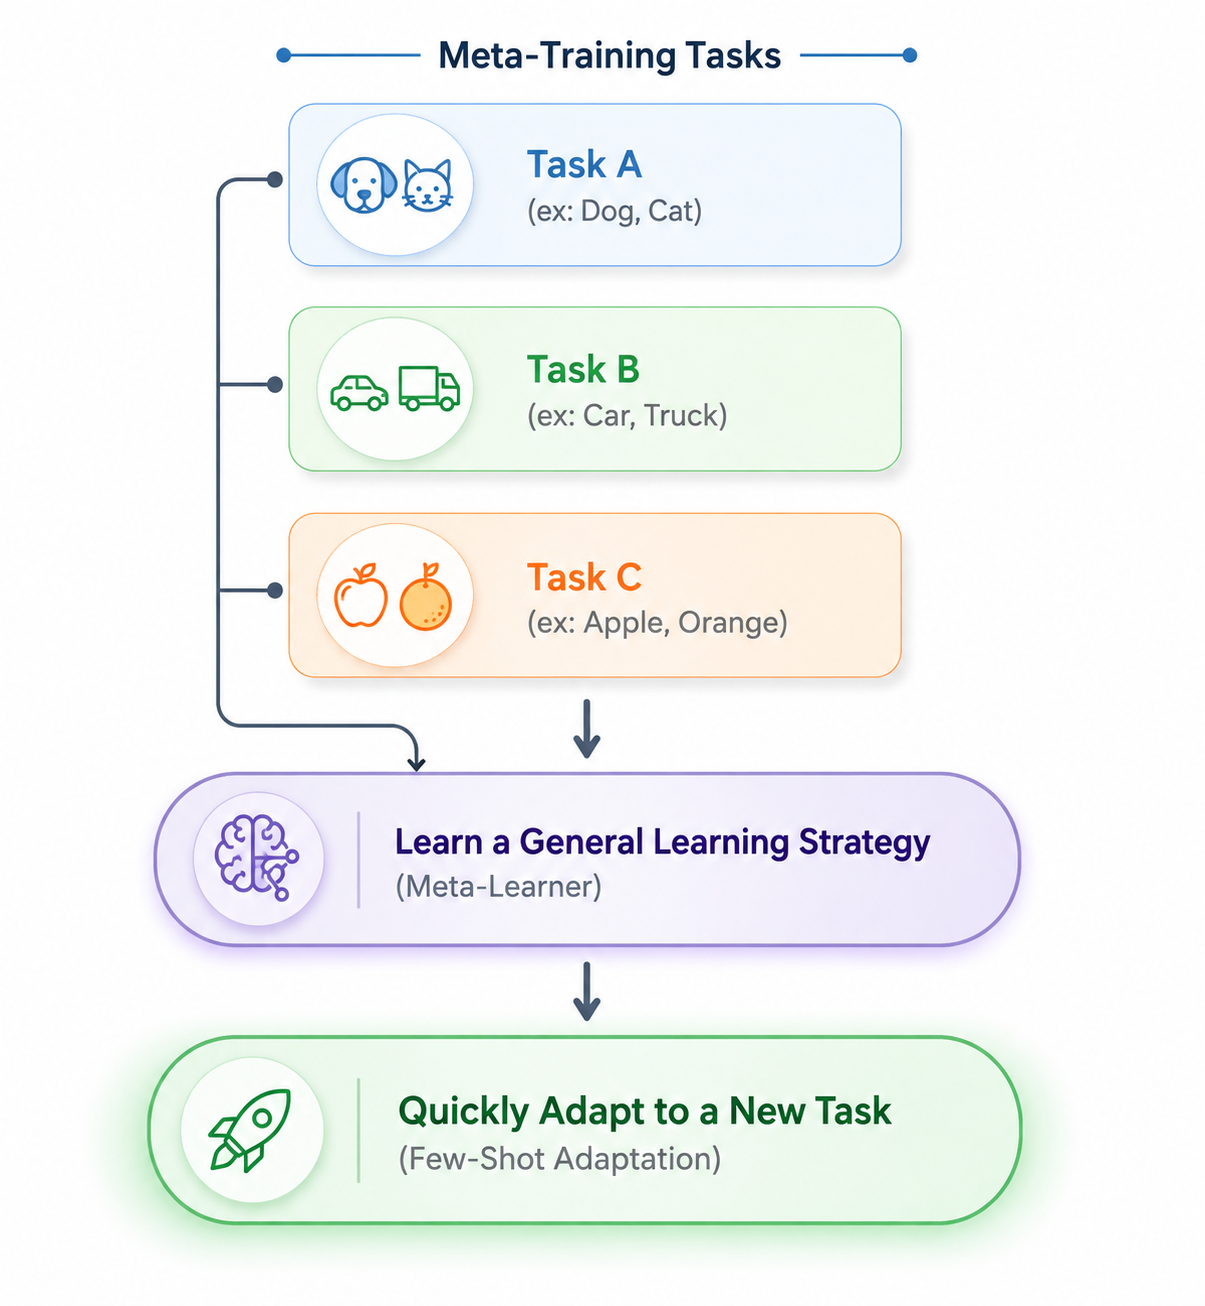
\includegraphics[width=0.85\textwidth]{figures/11-2 figure.png}
\caption{Meta-Learning Paradigm: Learning a General Strategy Across Multiple Meta-Training Tasks.}
\label{fig:meta_learning_concept}
\end{figure}

Unlike traditional deep learning which trains on one dataset for one task, Meta-Learning trains across many tasks:
\begin{itemize}
    \item \textbf{Task A} (ex: Dog, Cat)
    \item \textbf{Task B} (ex: Car, Truck)
    \item \textbf{Task C} (ex: Apple, Orange)
\end{itemize}

The model is trained on small tasks, not a single large dataset. Over time, it learns how to adapt quickly to new tasks independently.
The model continuously switches between tasks during training instead of training on one dataset. It learns patterns that help solve any new task.

\subsection*{Few-Shot Learning}

Meta-Learning is closely related to Few-Shot Learning:
\begin{itemize}
    \item \textbf{Zero-Shot}: No labeled examples of the target (new) classes.
    \item \textbf{One-Shot}: One labeled example per class.
    \item \textbf{Few-Shot}: A small number of labeled examples per class (typically 2--10).
    \item \textbf{Many-Shot}: Hundreds or thousands of labeled examples per class.
\end{itemize}

Traditional deep learning uses mini-batches. Instead, Meta-Learning training is divided into \textbf{episodes}:
\begin{itemize}
    \item \textbf{Episode 1}: Dogs, Cats
    \item \textbf{Episode 2}: Cars, Trucks
    \item \textbf{Episode 3}: Flowers
    \item \textbf{Episode 4}: Letters, Numbers
\end{itemize}
Thousands of episodes are used during training. Every episode teaches the model to solve a completely new task.

\vspace{0.5cm}
\subsection*{Inside Each Episode}

\textbf{Support Set}:
The first part is the Support Set. It contains the examples that the model is allowed to learn from. It is like a tiny training set.

\begin{figure}[H]
\centering
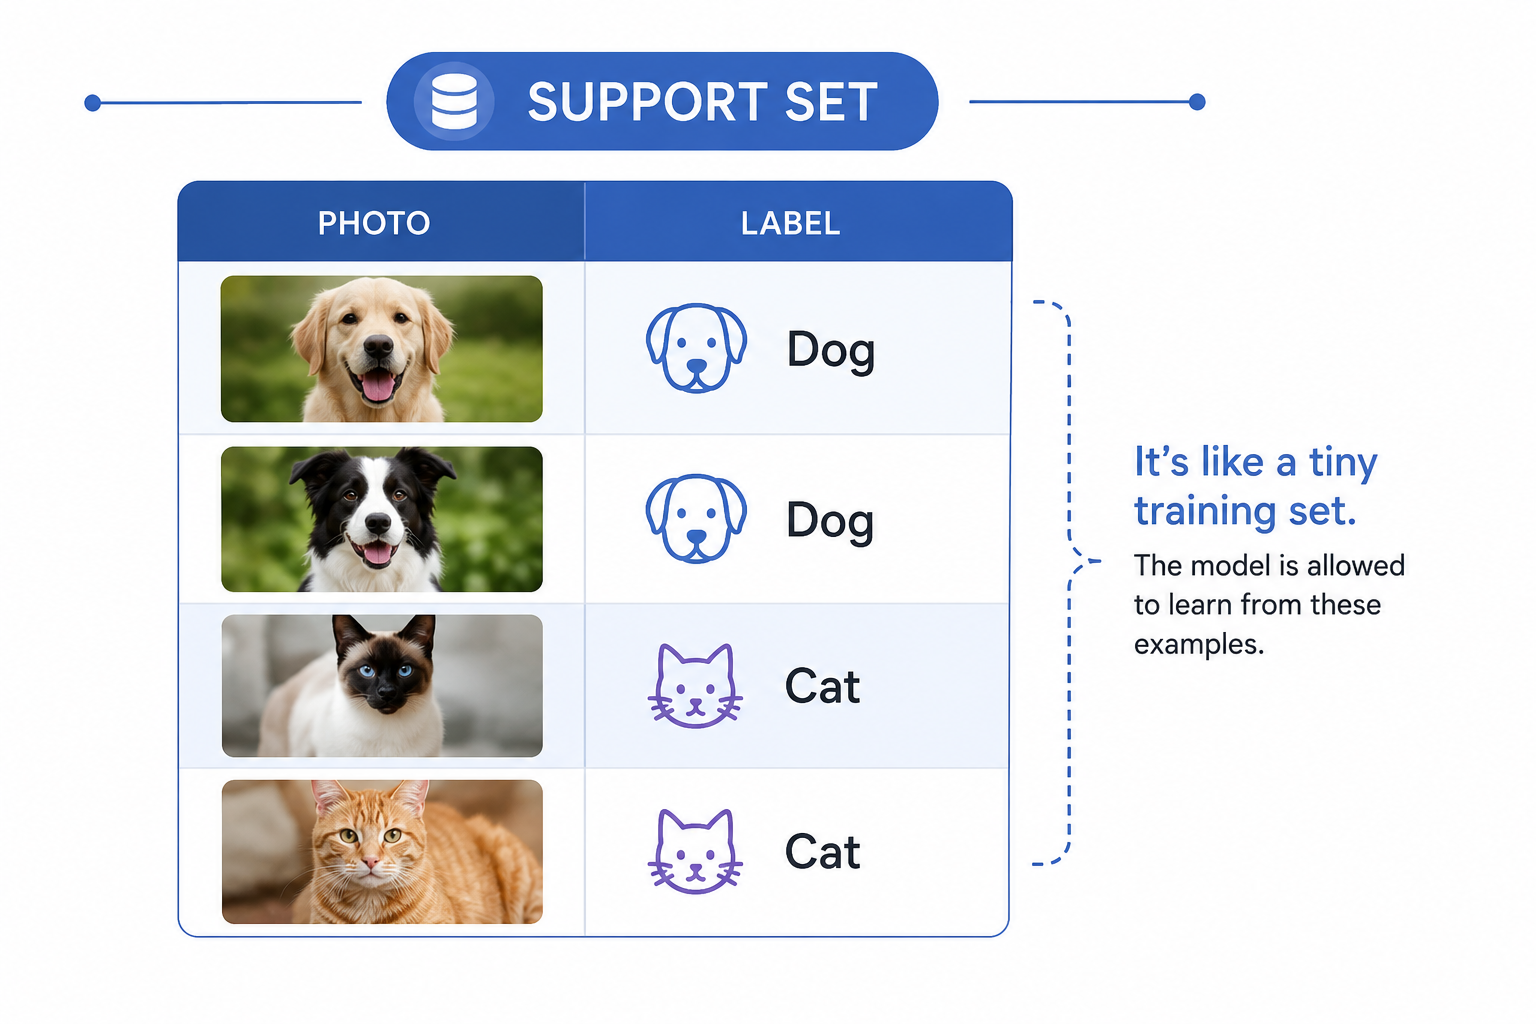
\includegraphics[width=0.85\textwidth]{figures/11-3 figure.png}
\caption{Support Set Structure inside an Episode.}
\label{fig:support_set}
\end{figure}

\textbf{Query Set}:
After studying the Support Set, the model is tested on the Query Set. The model must predict the labels using only what it learned from the Support Set. It is like a tiny test set.

\begin{figure}[H]
\centering
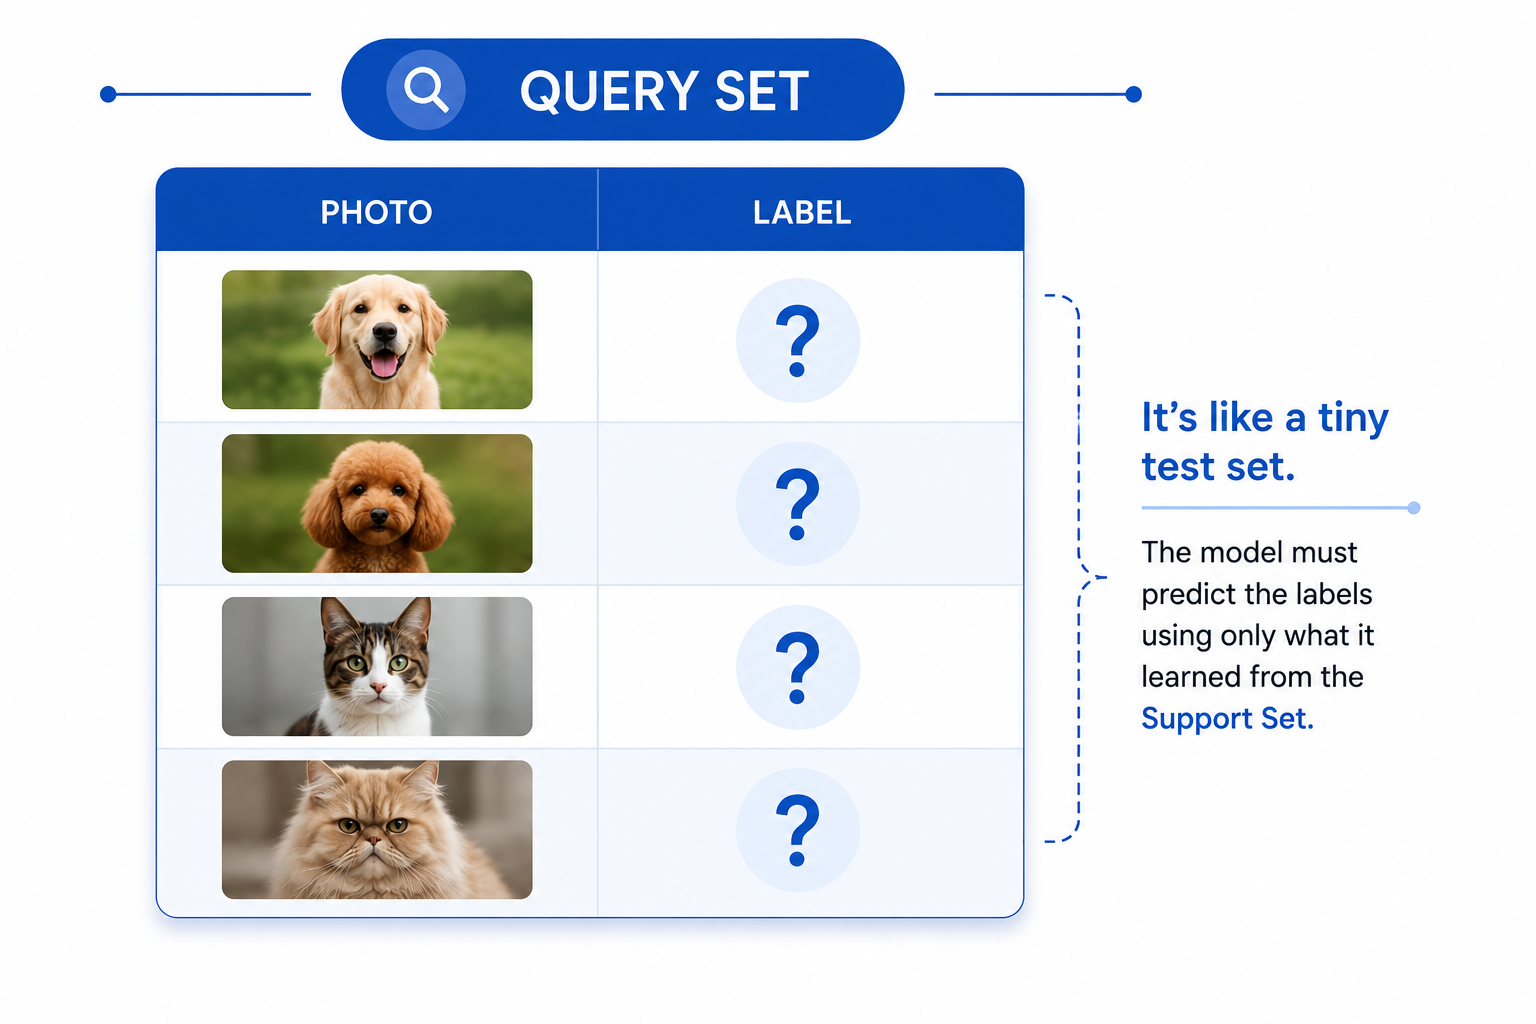
\includegraphics[width=0.85\textwidth]{figures/11-4 figure.png}
\caption{Query Set Structure inside an Episode.}
\label{fig:query_set}
\end{figure}

\subsubsection*{Complete Episode}

A complete episode consists of:
\begin{figure}[H]
\centering
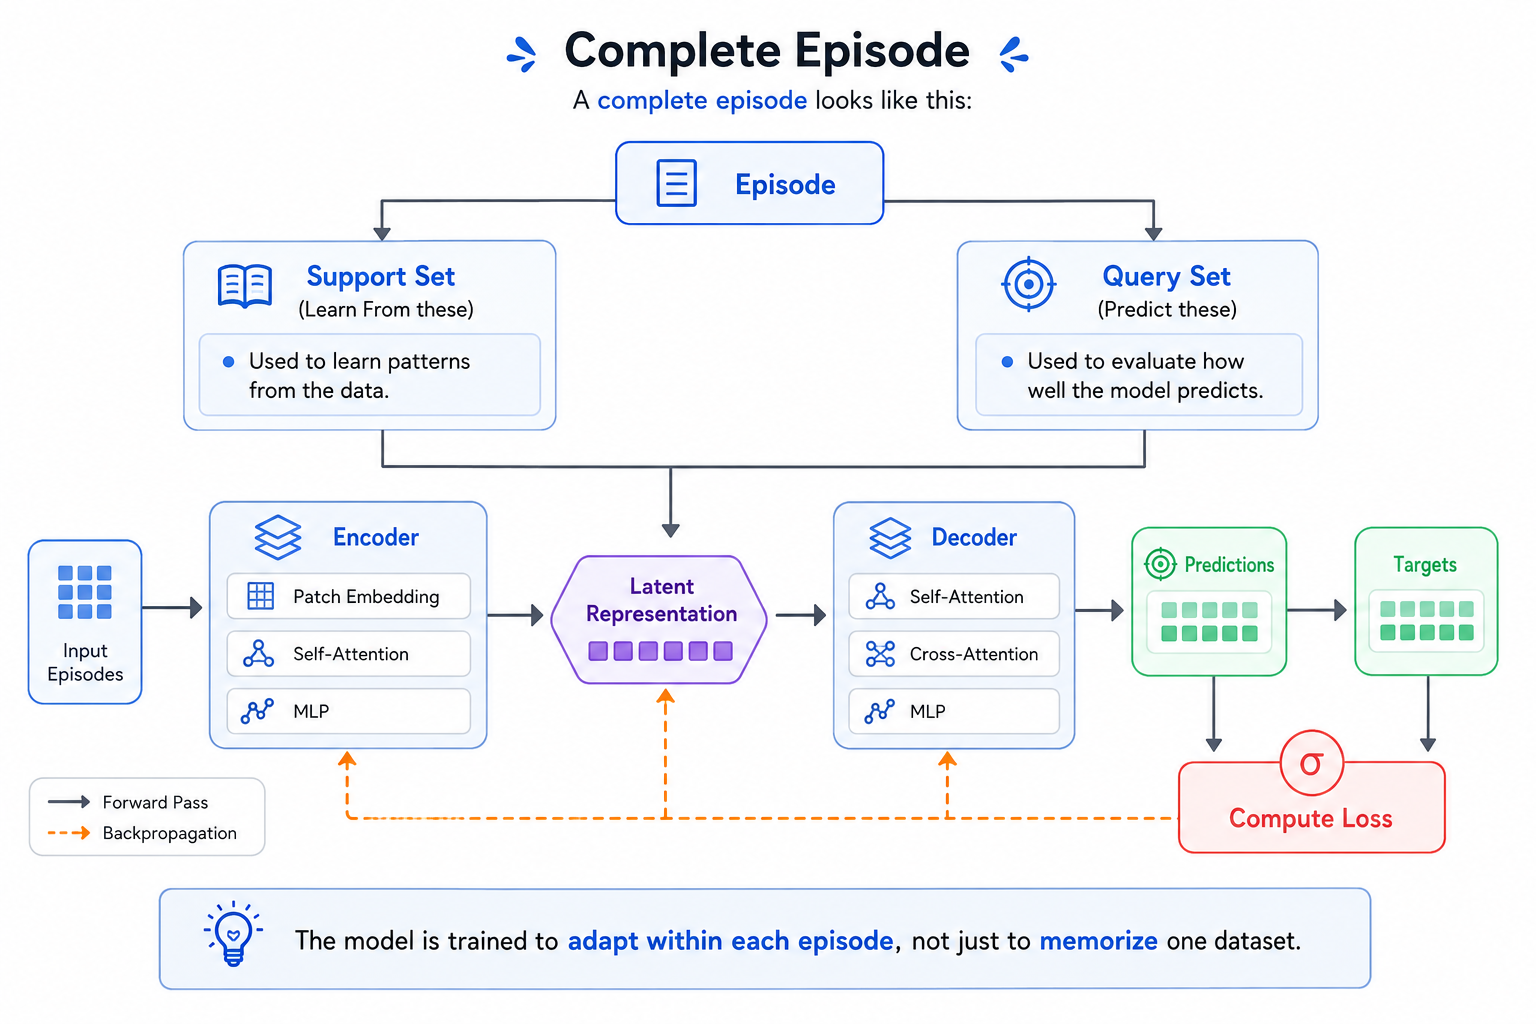
\includegraphics[width=0.95\textwidth]{figures/11-5 figure.png}
\caption{Complete Episode Flow.}
\label{fig:complete_episode}
\end{figure}

The model is trained to adapt within each episode, not just to memorize one dataset.

\subsection*{Meta-Learning Summary}

Meta-Learning addresses the limitation of traditional deep learning, which typically requires large labeled datasets for every new task. Instead of learning a single task, a meta-learning model is trained across many tasks, allowing it to ``Learn to Learn''.

Training is based on episodes, where each episode contains a Support Set (for learning) and a Query Set (for evaluation). This prepares the model to solve new tasks with only a few examples, making it particularly effective for Few-Shot Learning.

\section{Metric-Based Meta-Learning}

\subsection*{1) Siamese Networks}

Traditional Classifiers learn to predict fixed classes. However, in One-Shot or Few-Shot Learning, there are few labeled examples to train a reliable classifier.

Instead of learning ``what is this class?'', a Siamese Network asks: \textbf{``How similar are two inputs?''}

\textbf{Main Idea}: A Siamese Network consists of two identical sub-networks that share the same parameters. It takes two inputs and predicts whether they belong to the same class or different classes.

\begin{figure}[H]
\centering
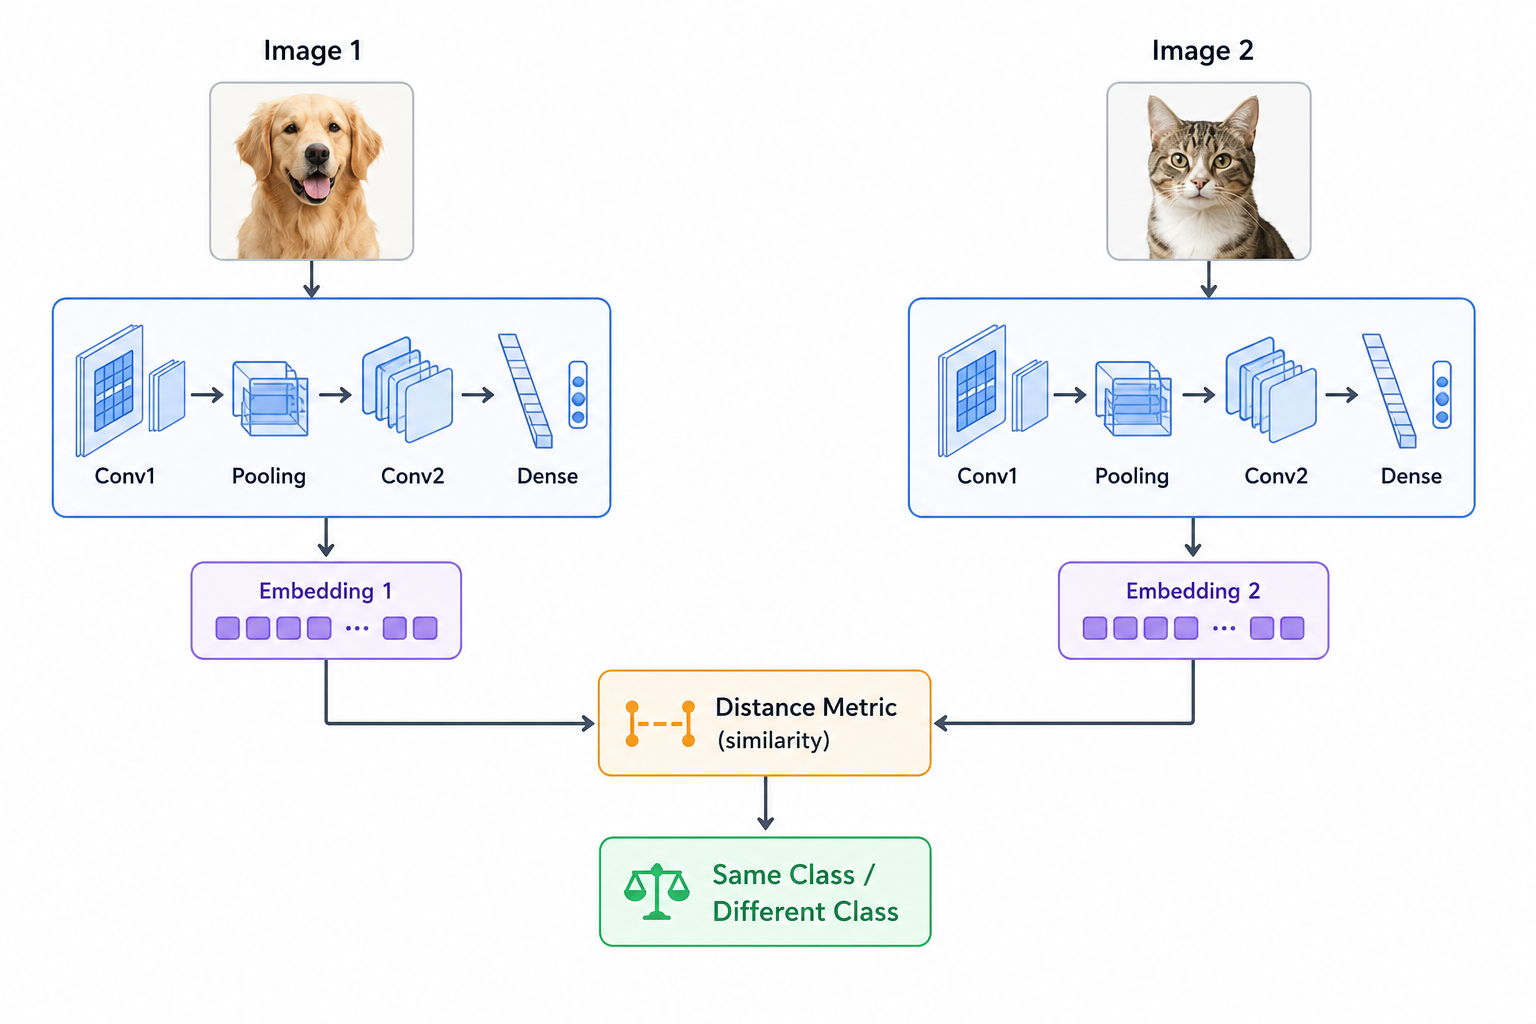
\includegraphics[width=0.95\textwidth]{figures/11-6-1 figure.png}
\caption{Siamese Network Architecture.}
\label{fig:siamese_network}
\end{figure}

The twin networks share the same weights so that both inputs are mapped into the same embedding space and their features are directly comparable.

Siamese Networks are typically trained with Contrastive Loss to pull positive pairs (same class) closer together and push negative pairs (different classes) farther apart.

\textbf{One-Shot Classification}:
When a query image has never been seen before and we only have one support image per class, the query is passed into the Siamese Network with each support image. If the distance is small, the model predicts that class. No retraining needed.

\textbf{Advantages}:
\begin{itemize}
    \item Works with very few examples per class.
    \item No need to retrain the classifier for new classes.
\end{itemize}

\textbf{Limitations}:
\begin{itemize}
    \item Compares image pairs, which means evaluation grows pairwise with many support examples.
    \item Does not create a representative prototype for each class.
\end{itemize}

\subsection*{2) Matching Networks}

In Siamese Networks, classification is performed by comparing individual pairs. Each comparison (Query -- every individual support example) is independent; the model never considers the support set as a whole.

Researchers asked: ``Can the prediction depend on all support images simultaneously?'' This led to Matching Networks.

\textbf{Main Idea}: A query and all support images are first encoded into a common embedding space using a Shared Encoder.

The query embedding is then compared with every support embedding using a similarity measure (Cosine Similarity). The similarities are converted into attention-like weights using Softmax.

The class prediction is obtained as a weighted combination of the support labels, where more similar support examples contribute more to the final prediction.

\begin{figure}[H]
\centering
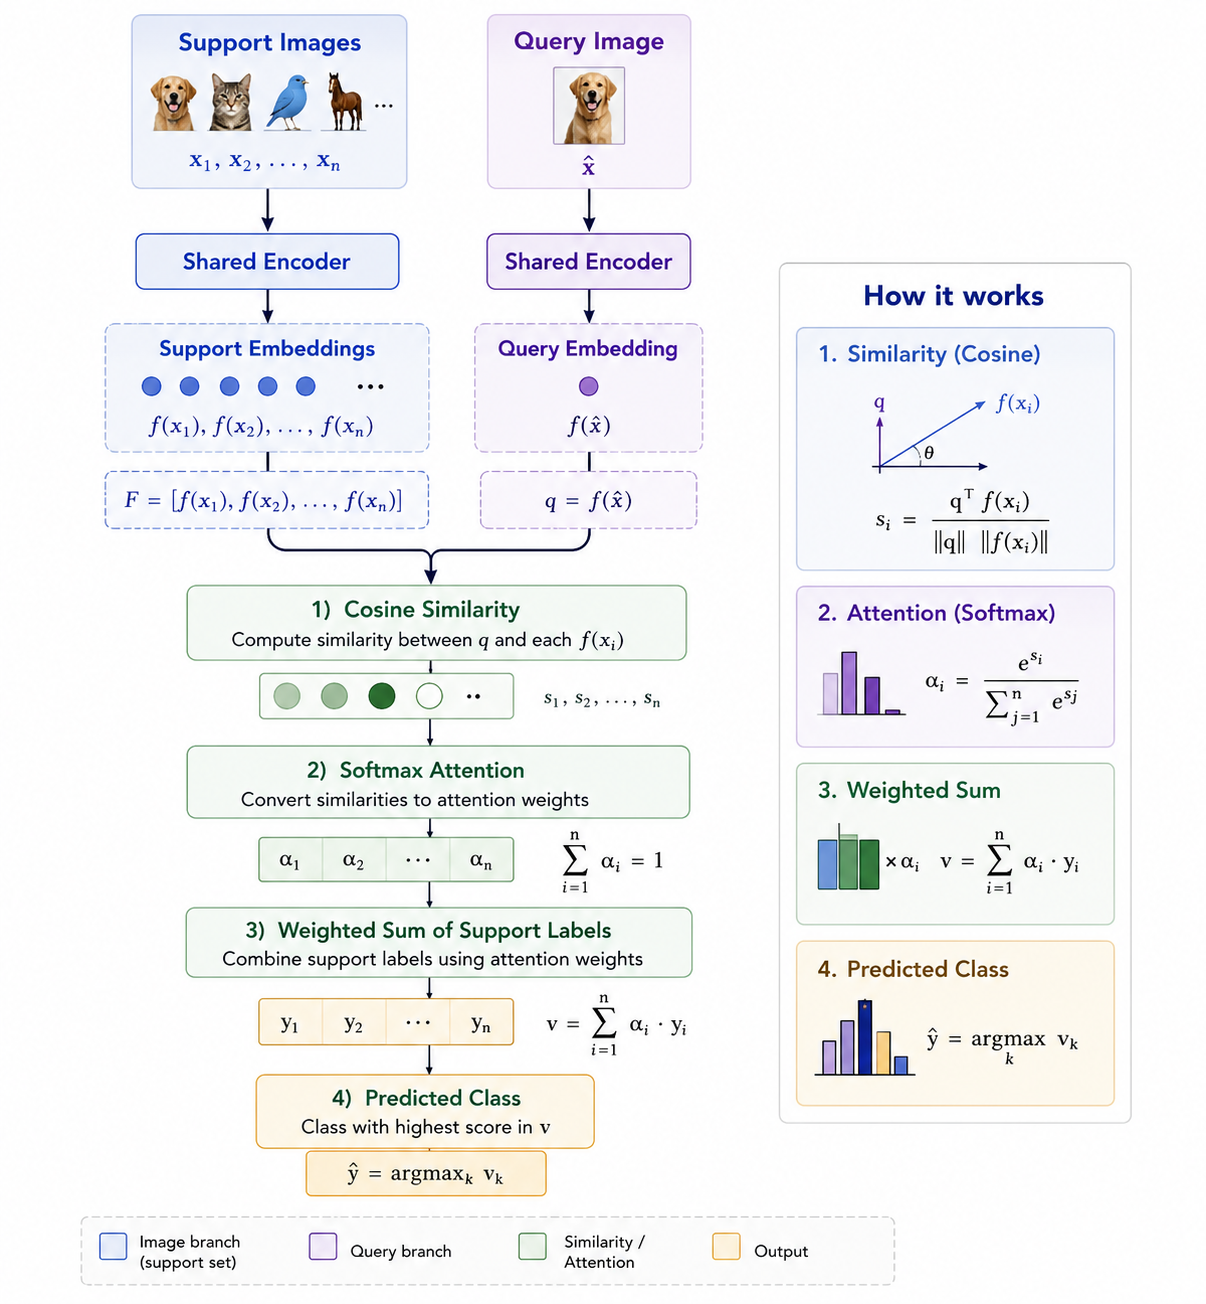
\includegraphics[width=0.95\textwidth]{figures/11-6 figure.png}
\caption{Matching Network Architecture.}
\label{fig:matching_network}
\end{figure}

\textbf{Matching Networks Pipeline}:
\begin{enumerate}
    \item \textbf{Shared Encoder}: Maps both support images and query image to the same embedding space.
    \item \textbf{Cosine Similarity}: Measures similarity between query embedding and each support embedding.
    \item \textbf{Softmax Attention}: Converts similarities to attention weights that sum to 1.
    \item \textbf{Weighted Sum of Labels}: Combines support labels using attention weights.
    \item \textbf{Predicted Class}: Selects the class with the highest score in the weighted sum.
\end{enumerate}

\textbf{Episodic Training}:
Matching Networks introduced an important training strategy: training using episodes, exactly like testing. Each episode contains a Support Set and a Query Set. This teaches the model to solve the same type of few-shot tasks it will encounter during inference.

\textbf{Advantages}:
\begin{itemize}
    \item Uses the entire support set as context instead of isolated pairs.
    \item Naturally handles different support set sizes.
    \item Better few-shot performance than Siamese Networks.
\end{itemize}

\textbf{Limitations}:
\begin{itemize}
    \item Every query must be compared with every support example. When support set size grows, computational cost grows linearly.
    \item Stores individual support embeddings rather than compact class prototypes.
\end{itemize}

\subsection*{3) Prototypical Networks}

In Matching Networks, classifying a query requires comparing it with every support image. If we have 100 support examples per class, the model must compare against 100 images per class.

Researchers asked: ``Do we really need every support example? Or can we store one representation vector per class?''

\textbf{Core Idea}: Instead of storing all support embeddings, Prototypical Networks compute a single Prototype vector for each class by taking the mean embedding of all support examples of that class.

\begin{figure}[H]
\centering
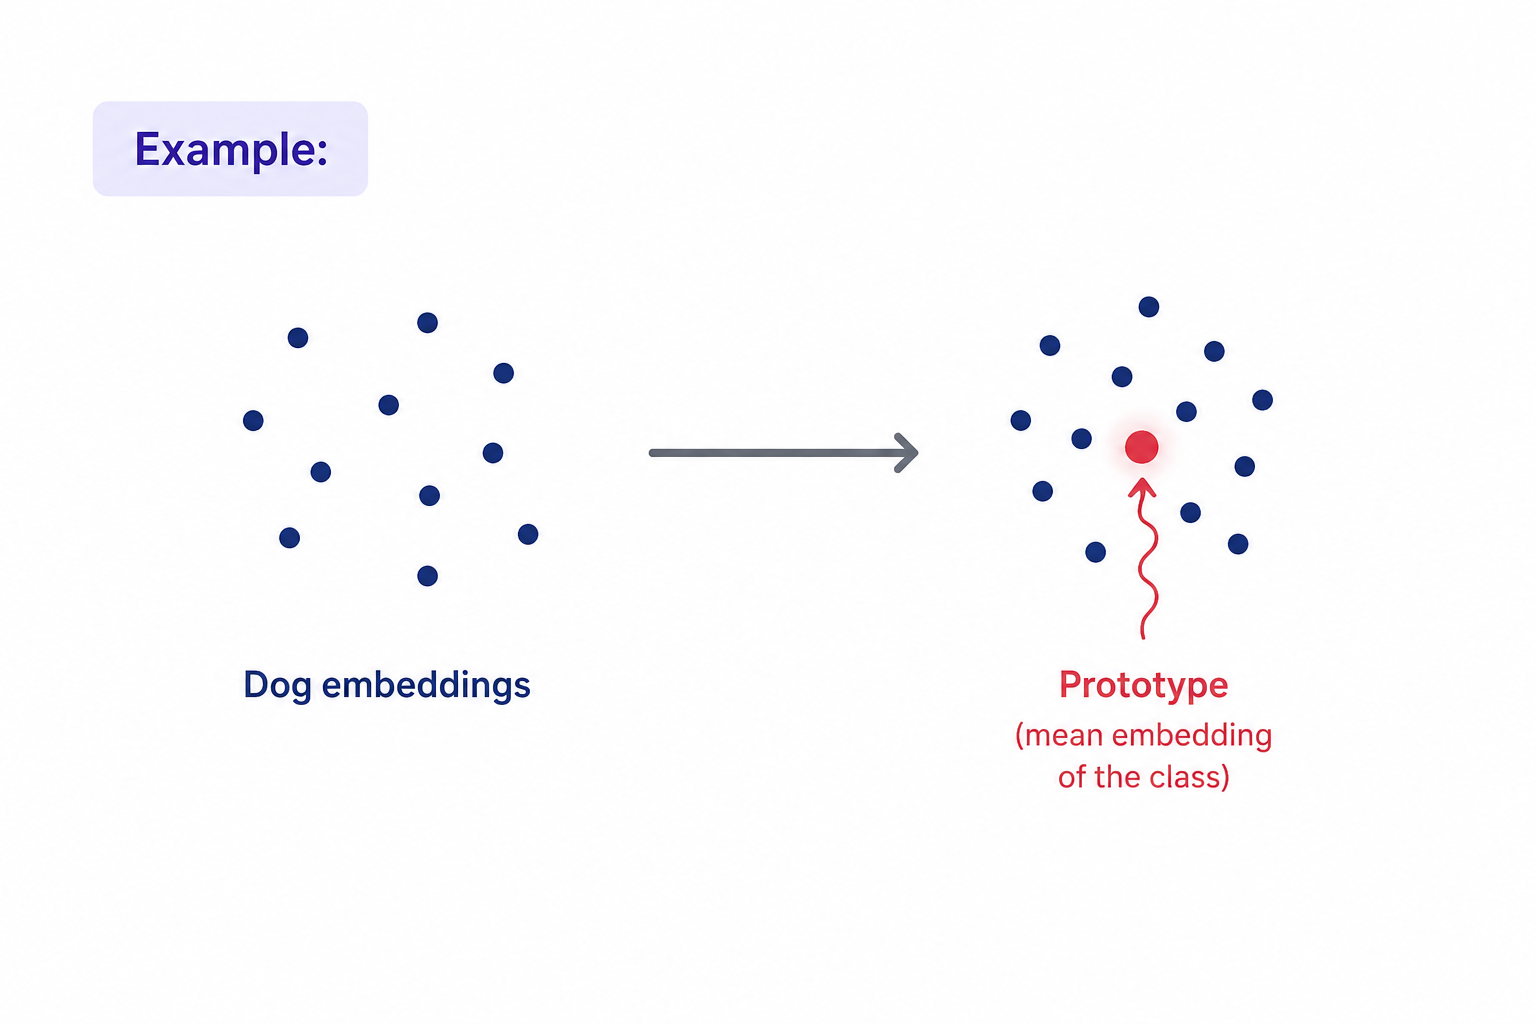
\includegraphics[width=0.85\textwidth]{figures/11-7 figure.png}
\caption{Class Prototypes in Feature Space.}
\label{fig:prototypes_concept}
\end{figure}

Now, every class is represented by one vector (Prototype).

\textbf{Architecture}
\begin{figure}[H]
\centering
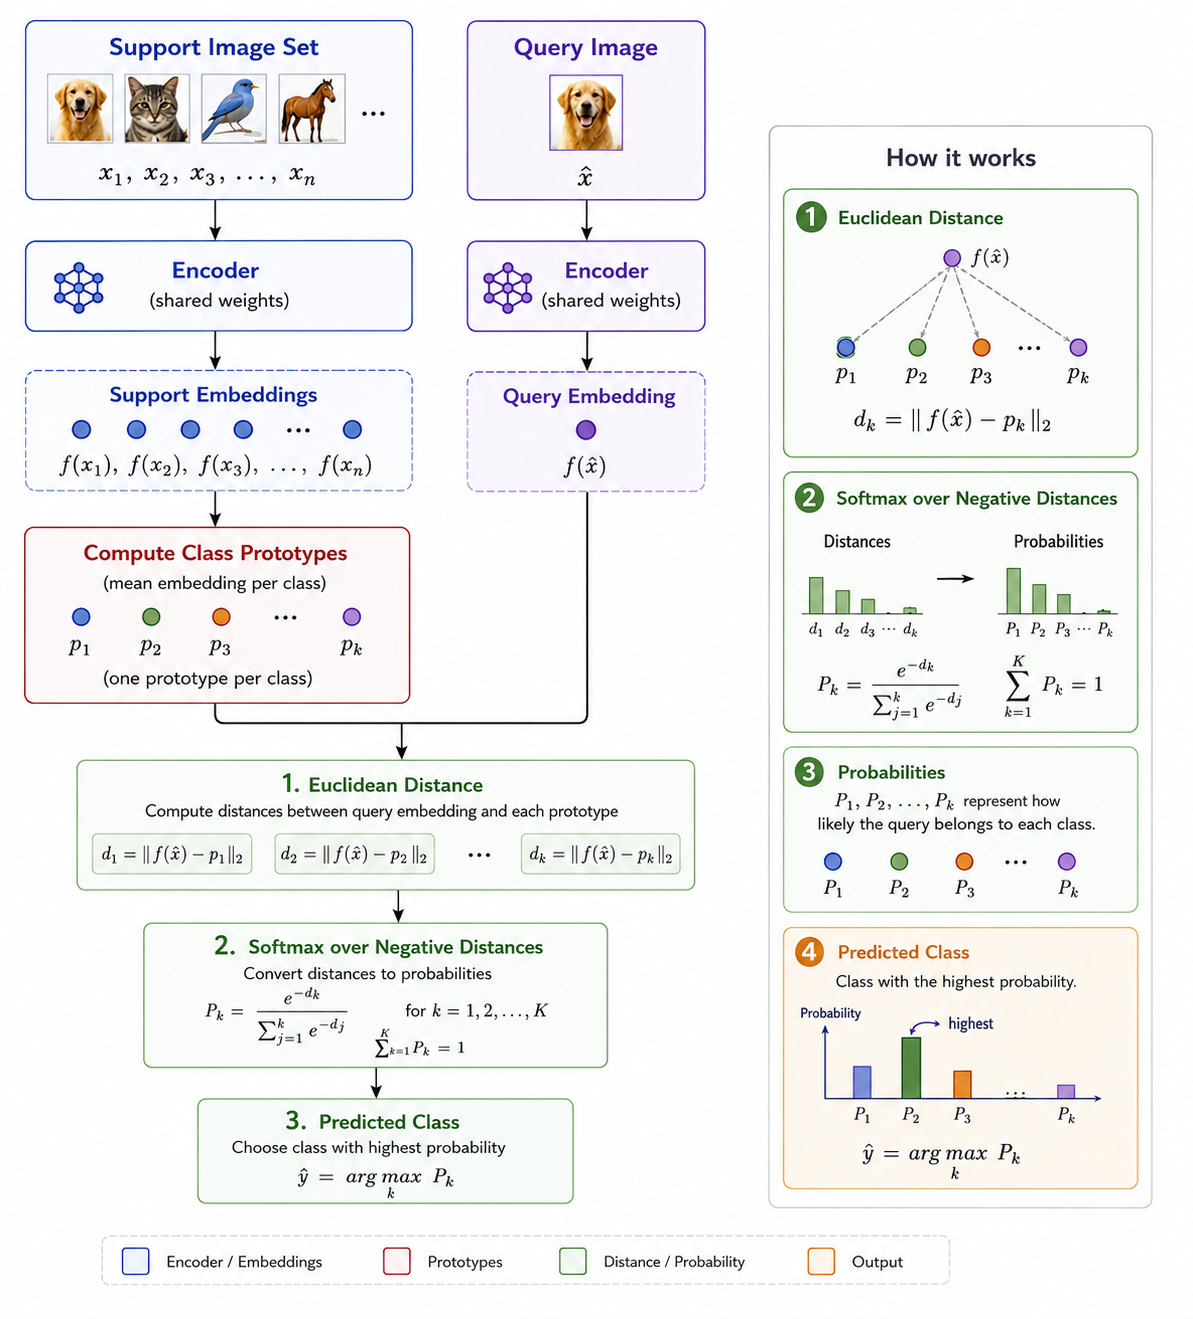
\includegraphics[width=0.80\textwidth]{figures/11-8 figure.png}
\caption{Computation of a Class Prototype as Mean Embedding.}
\label{fig:prototype_mean_embedding}
\end{figure}

During training, the encoder learns an embedding space where:
\begin{itemize}
    \item Samples belonging to the same class cluster together.
    \item Samples from different classes are naturally separated.
\end{itemize}

\begin{figure}[H]
\centering
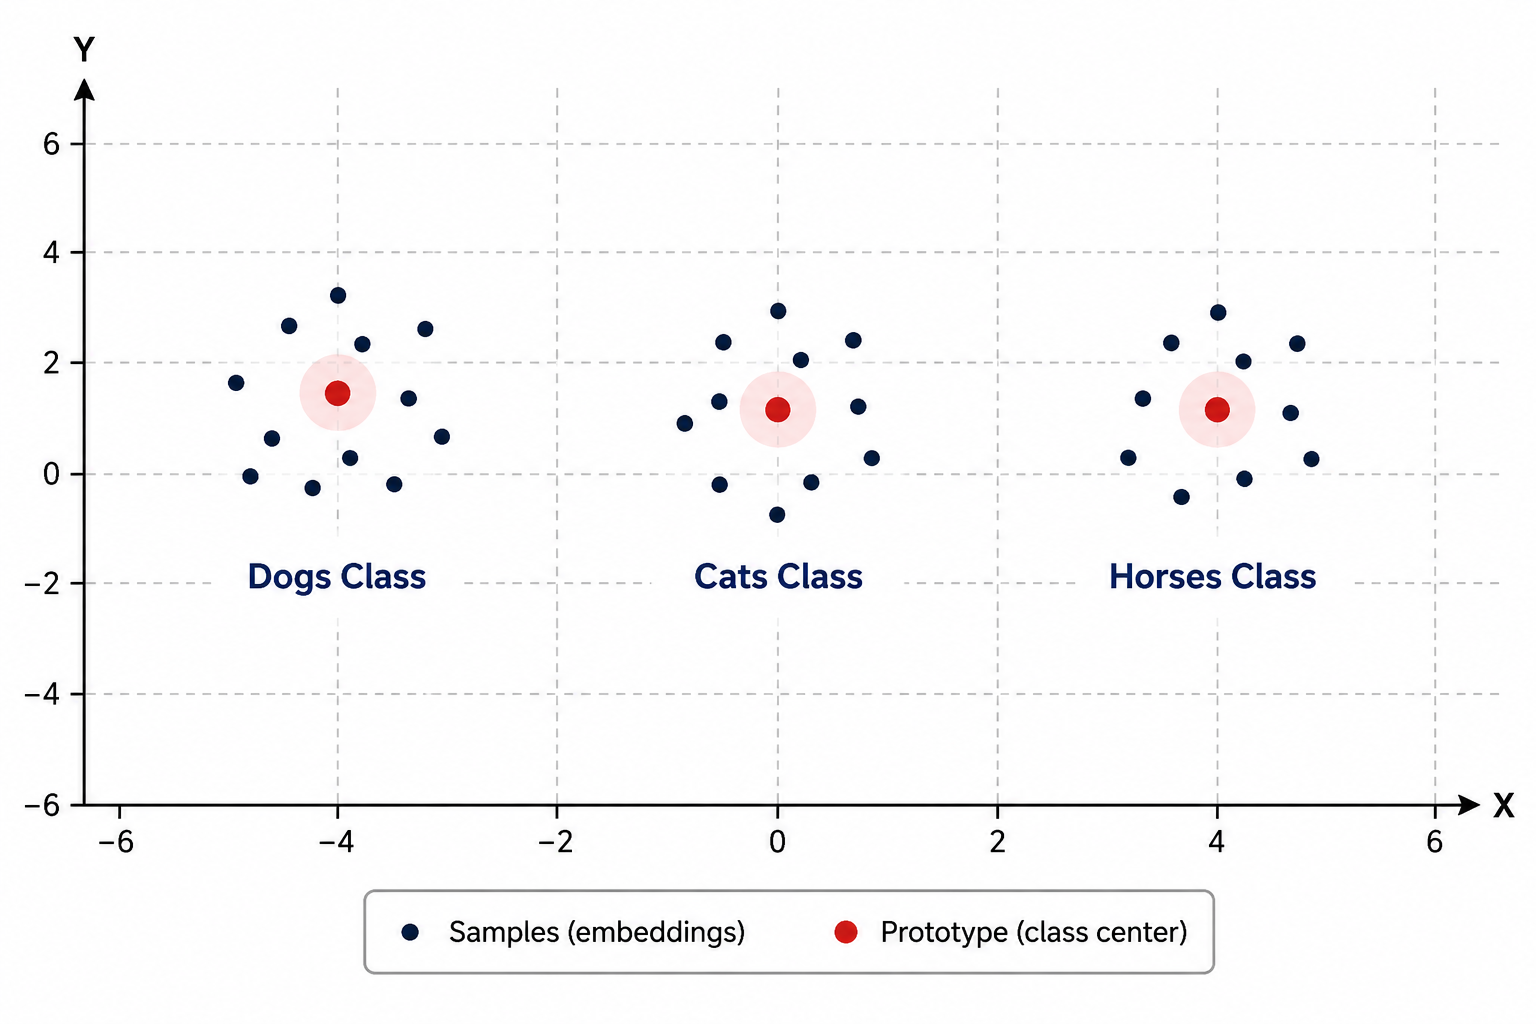
\includegraphics[width=0.95\textwidth]{figures/11-9 figure.png}
\label{fig:prototypical_networks}
\end{figure}

If the embedding space is well learned, the Prototype becomes an excellent representative of its class.

\textbf{How it works}:
\begin{enumerate}
    \item \textbf{Compute Prototypes}: $p_k = \frac{1}{|S_k|} \sum_{x_i \in S_k} f(x_i)$.
    \item \textbf{Euclidean Distance}: Compute distance $d_k = \|f(\hat{x}) - p_k\|^2$.
    \item \textbf{Softmax over Distances}: $P(y = k \mid \hat{x}) = \frac{\exp(-d_k)}{\sum_{k'} \exp(-d_{k'})}$.
    \item \textbf{Predicted Class}: $\hat{y} = \text{argmax}_k P(y = k \mid \hat{x})$.
\end{enumerate}

The encoder learns an embedding space where samples of the same class cluster together and different classes naturally separate.

\textbf{Advantages}:
\begin{itemize}
    \item Simple and fast inference (one comparison per class instead of every image).
    \item Excellent few-shot performance.
\end{itemize}

\textbf{Limitations}:
\begin{itemize}
    \item Assumes each class can be represented by a single center (mean prototype). This assumption fails when classes have complex, multimodal distributions.
\end{itemize}

\begin{figure}[H]
\centering
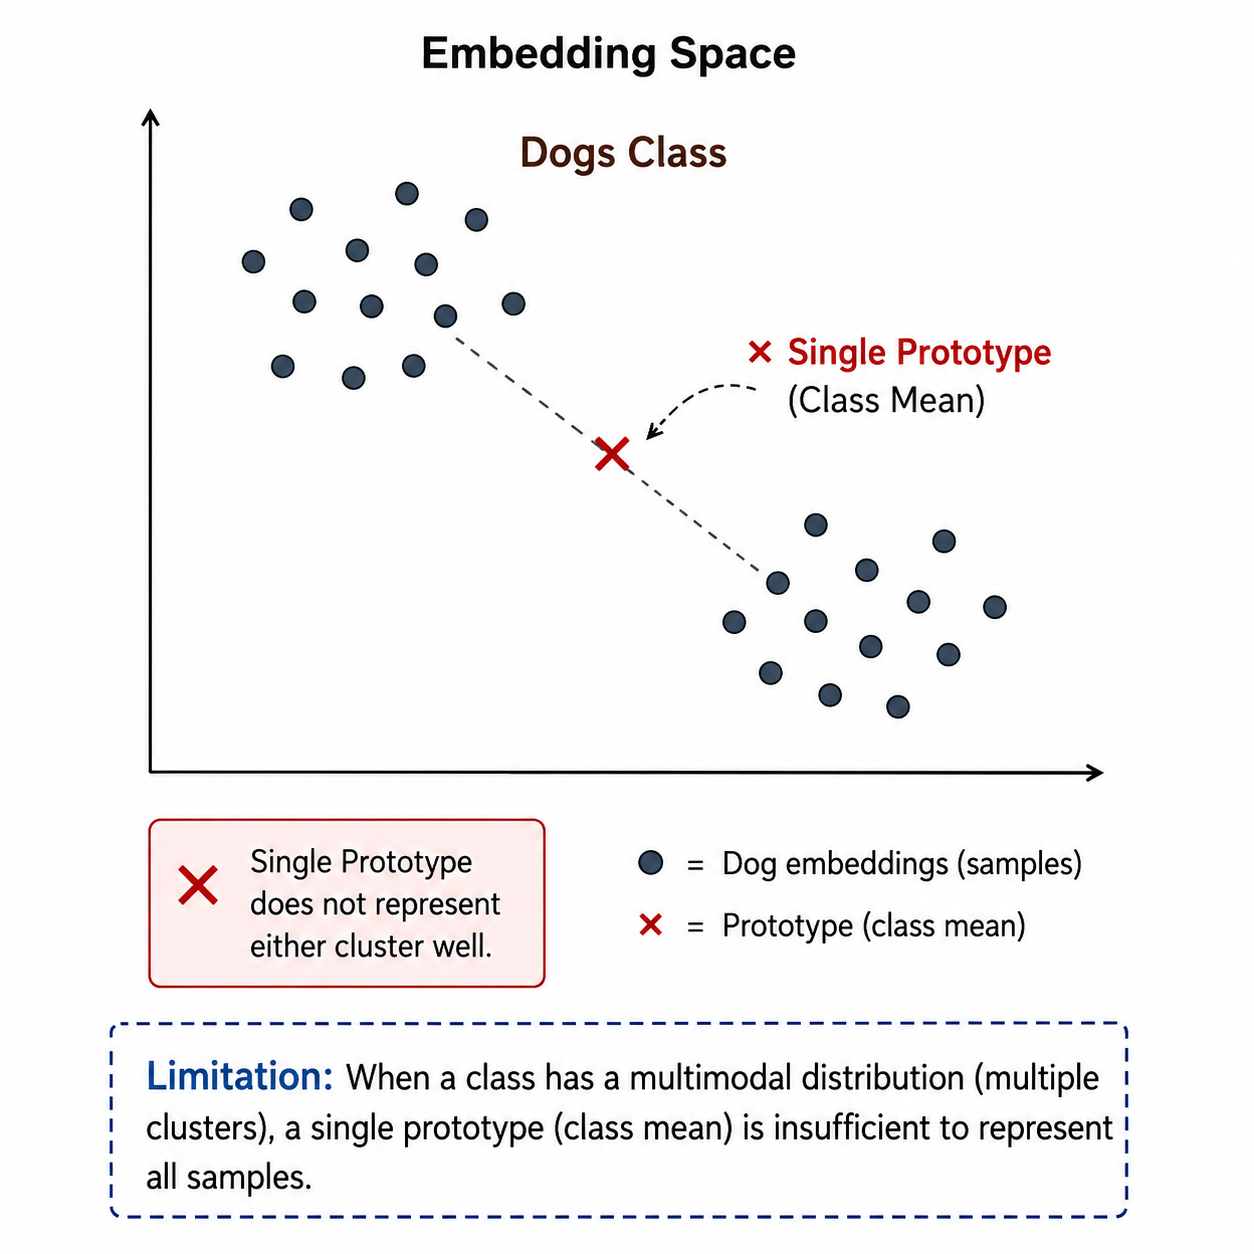
\includegraphics[width=0.95\textwidth]{figures/11-10 figure.png}
\caption{Prototypical Networks Architecture Detail.}
\label{fig:prototypical_networks_detail}
\end{figure}

\subsection*{4) Relation Networks}

In Prototypical Networks, the similarity function is fixed (Euclidean distance).

Researchers asked: ``Why should we manually choose Euclidean or Cosine distance? Can a neural network learn the similarity function itself?''

\textbf{Main Idea}: Relation Networks split the model into two learnable parts:
\begin{enumerate}
    \item \textbf{Embedding Network}: Extracts feature embeddings from images.
    \item \textbf{Relation Network}: A neural network module that outputs a similarity score between 0 and 1 for concatenated support and query feature maps $[s, q]$.
\end{enumerate}

\begin{figure}[H]
\centering
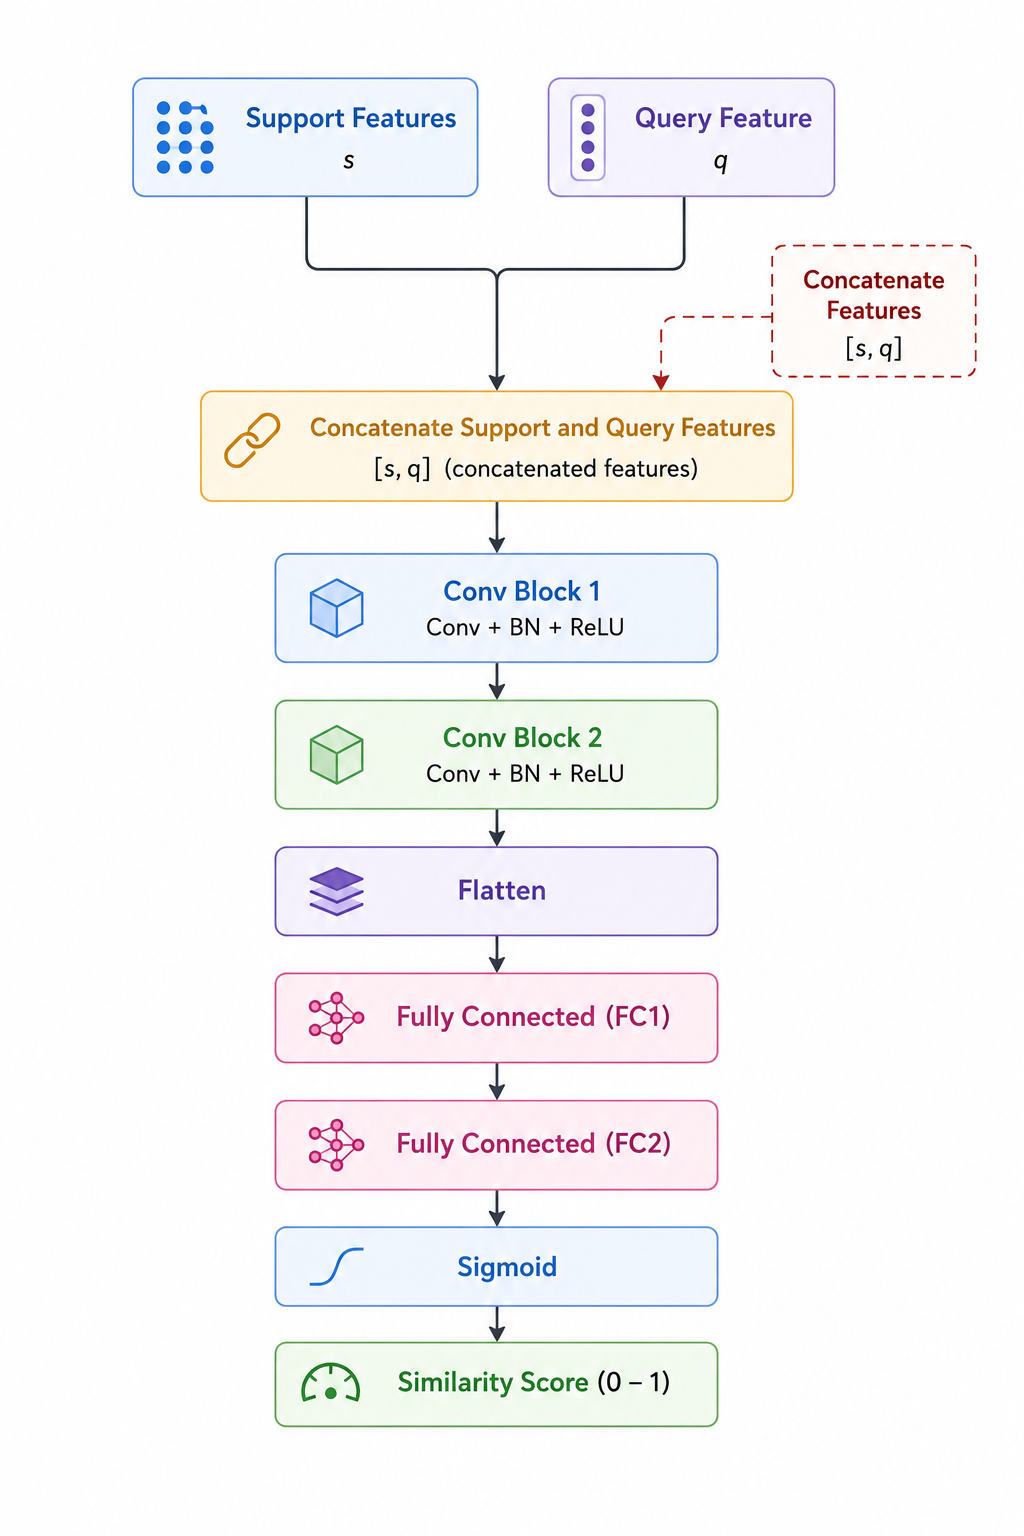
\includegraphics[width=0.95\textwidth]{figures/11-11 figure.png}
\caption{Relation Networks Architecture.}
\label{fig:relation_networks}
\end{figure}

The relation score produced by this network represents how similar the support and query features are.

\begin{figure}[H]
\centering
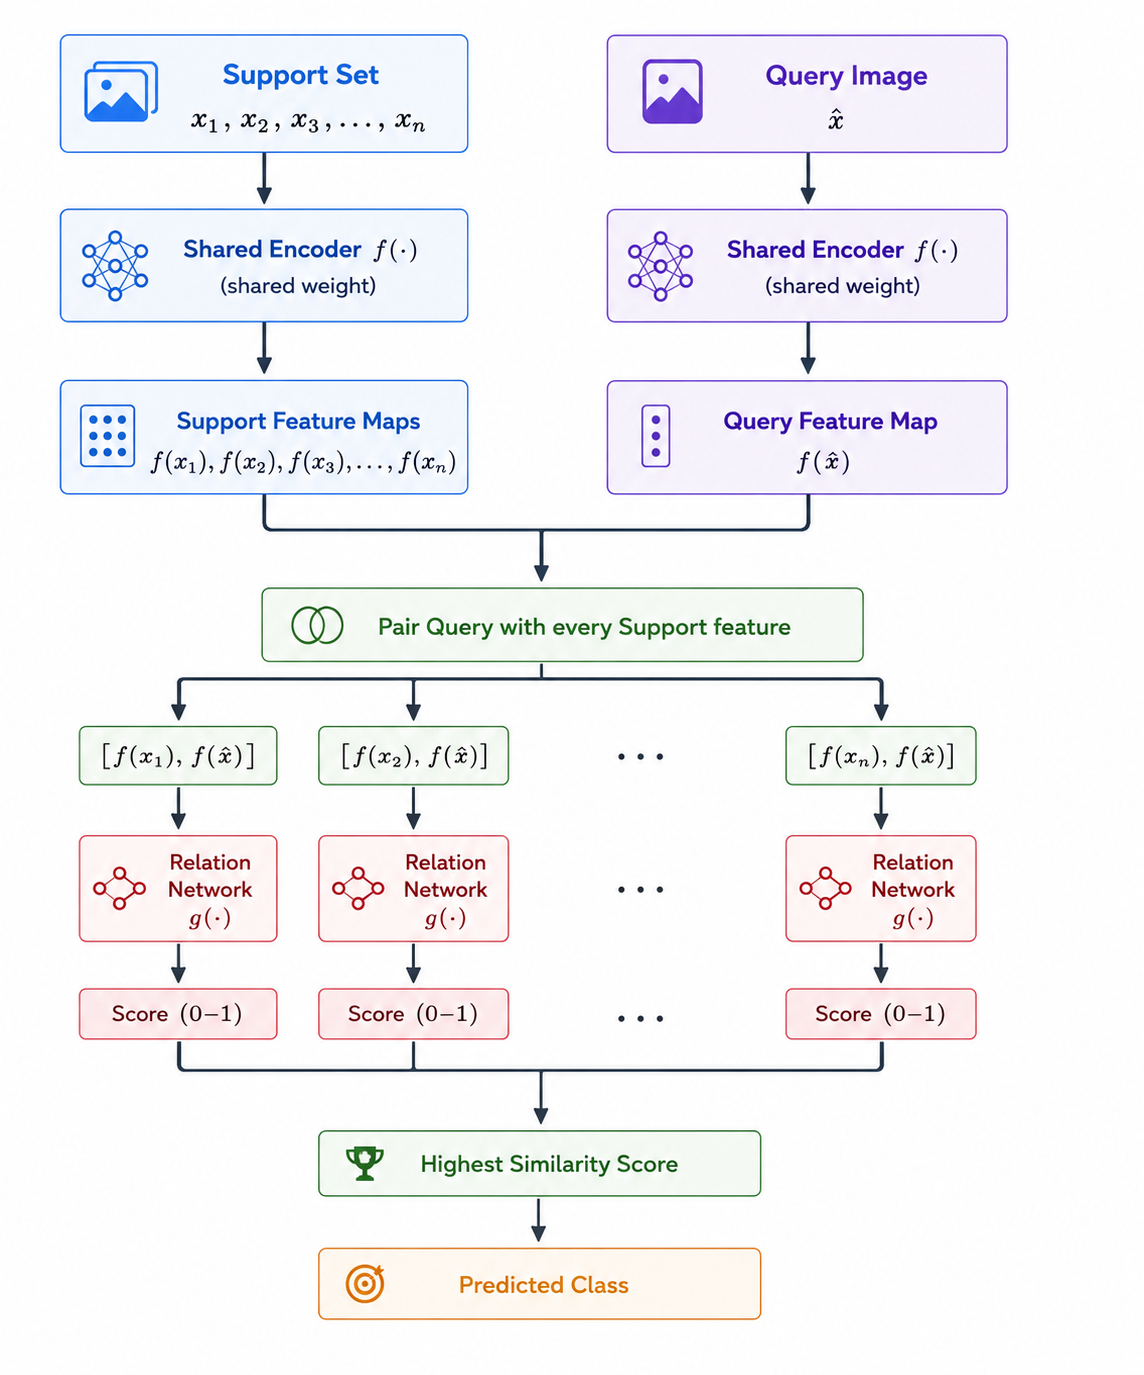
\includegraphics[width=0.75\textwidth]{figures/11-12 figure.png}
\label{fig:relation_module}
\end{figure}

Instead of fixed $\text{Distance}(z_1, z_2)$, we learn $\text{Relation}(z_1, z_2)$ using a Relation Network module.

The Euclidean distance assumes that similarity decreases linearly with distance. However, this assumption is not always valid. Two embeddings may exhibit:

\begin{itemize}
    \item Similar structural patterns.
    \item Correlated features.
    \item Complex nonlinear relationships that cannot be adequately captured by the Euclidean distance.
\end{itemize}

Instead, a learned relation function can automatically discover these underlying patterns and provide a more flexible measure of similarity.

\textbf{Advantages}:
\begin{itemize}
    \item Learns the similarity function instead of relying on a fixed metric.
    \item More flexible than Euclidean distance; can model complex relationships between embeddings.
\end{itemize}

\textbf{Limitations}:
\begin{itemize}
    \item Introduces additional parameters in the relation module.
    \item Higher computational cost and risk of overfitting compared to simple metric-based methods.
\end{itemize}

\section{Optimization-Based Meta-Learning}

\subsection*{Model-Agnostic Meta-Learning (MAML)}

Unlike metric-based methods that learn an embedding space, MAML learns an initial set of model parameters $\theta$ such that, after only a few gradient updates (typically 1--5), the model can rapidly adapt to a new task and achieve high performance.

\begin{figure}[H]
\centering
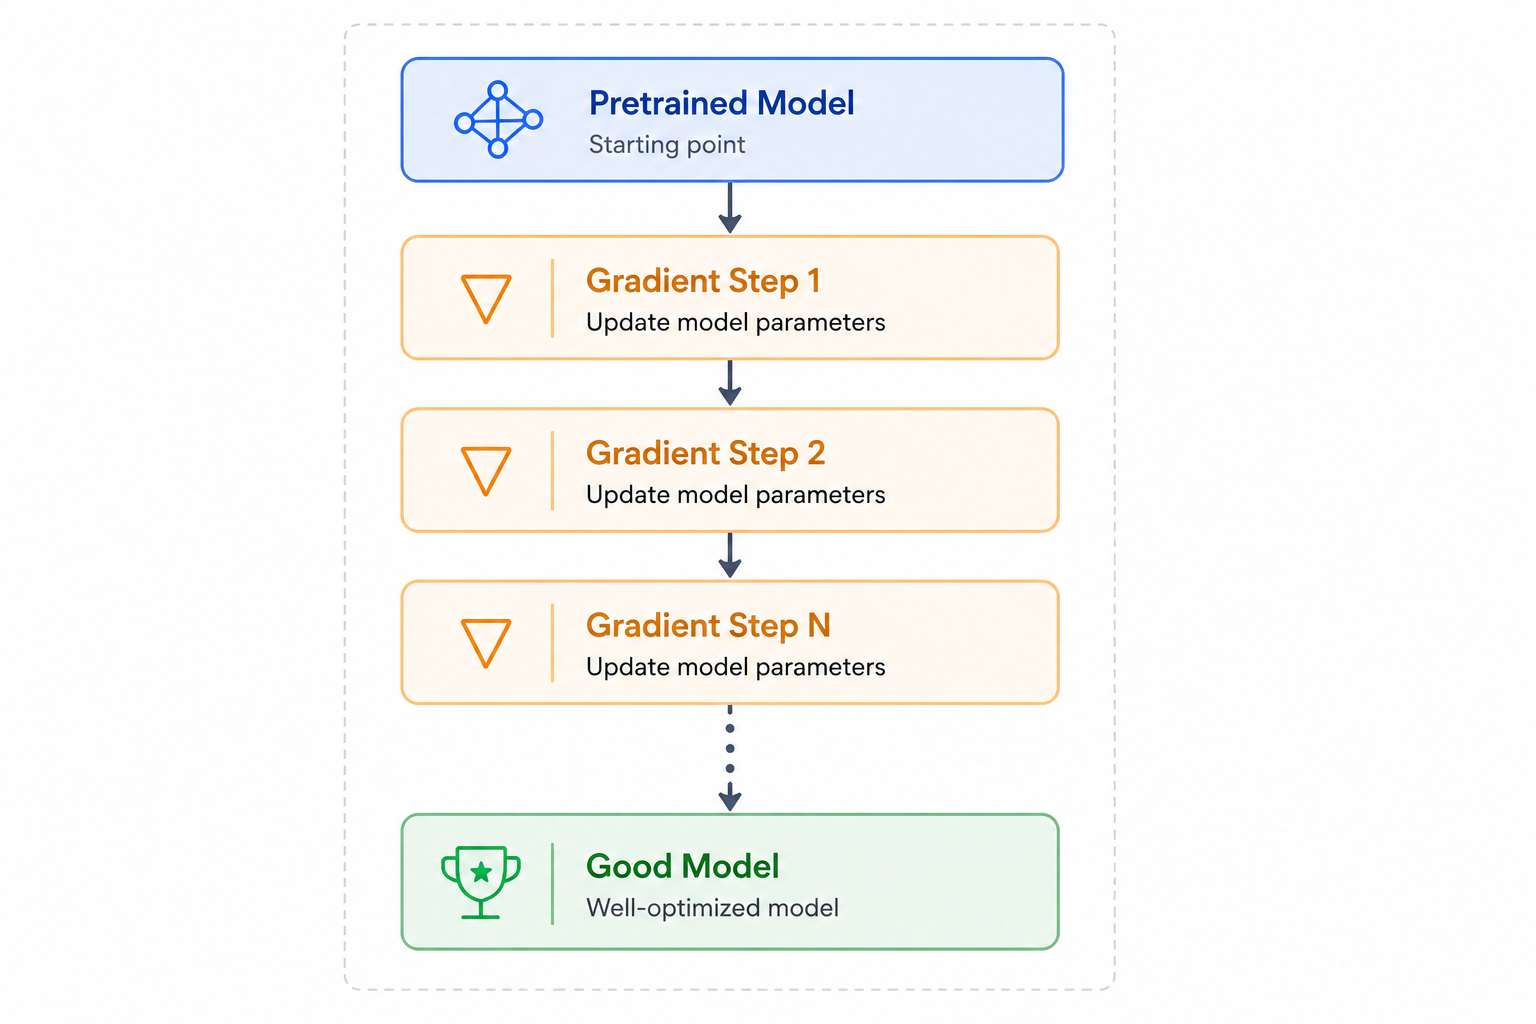
\includegraphics[width=0.65\textwidth]{figures/11-13 figure.png}
\end{figure}

Conventional deep learning models often require hundreds or even thousands of gradient updates to adapt to a new task. In contrast, MAML optimizes the initial parameters so that only a few gradient updates are sufficient for effective adaptation.

\begin{figure}[H]
\centering
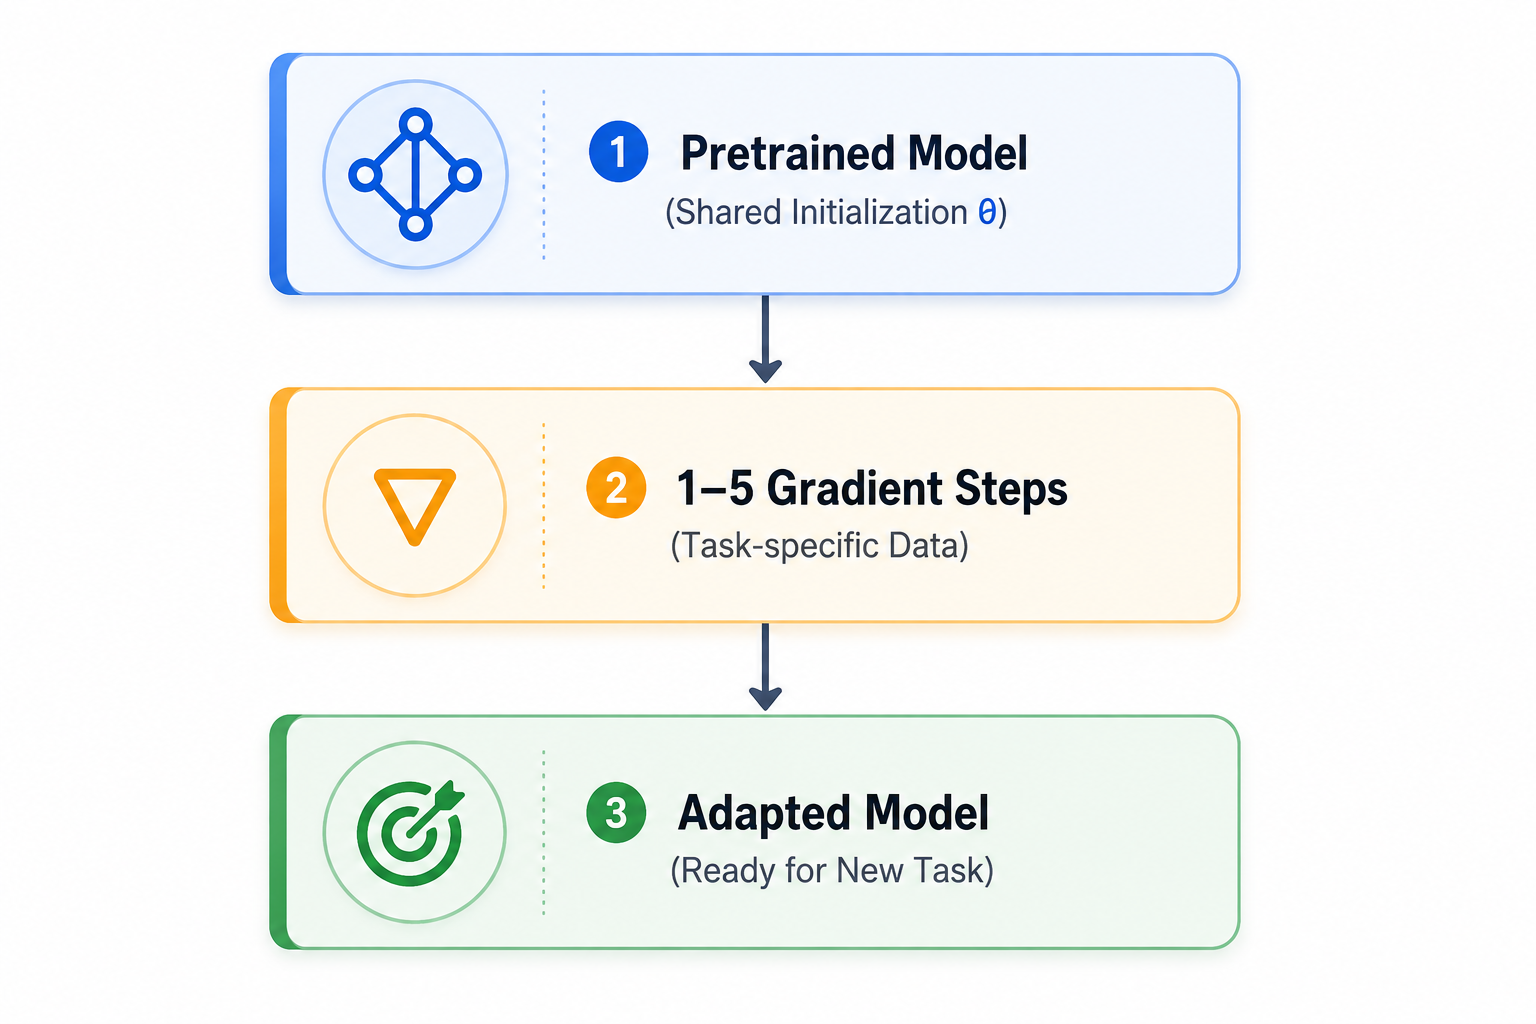
\includegraphics[width=0.65\textwidth]{figures/11-14 figure.png}
\end{figure}

In other words, MAML trains the model to be easy to fine-tune.
\vspace{3cm}
\subsubsection*{Core Idea of MAML}

The goal of MAML is to find an initial parameter vector $\theta$ such that for any new task $\mathcal{T}_i$, the model achieves good performance after taking just $1$--$5$ gradient steps.

Instead of learning a static representation, MAML explicitly optimizes for fast task adaptation.

Like previous meta-learning methods, MAML trains across a set of tasks $\{\mathcal{T}_i\}$ rather than a single dataset.

\begin{figure}[H]
\centering
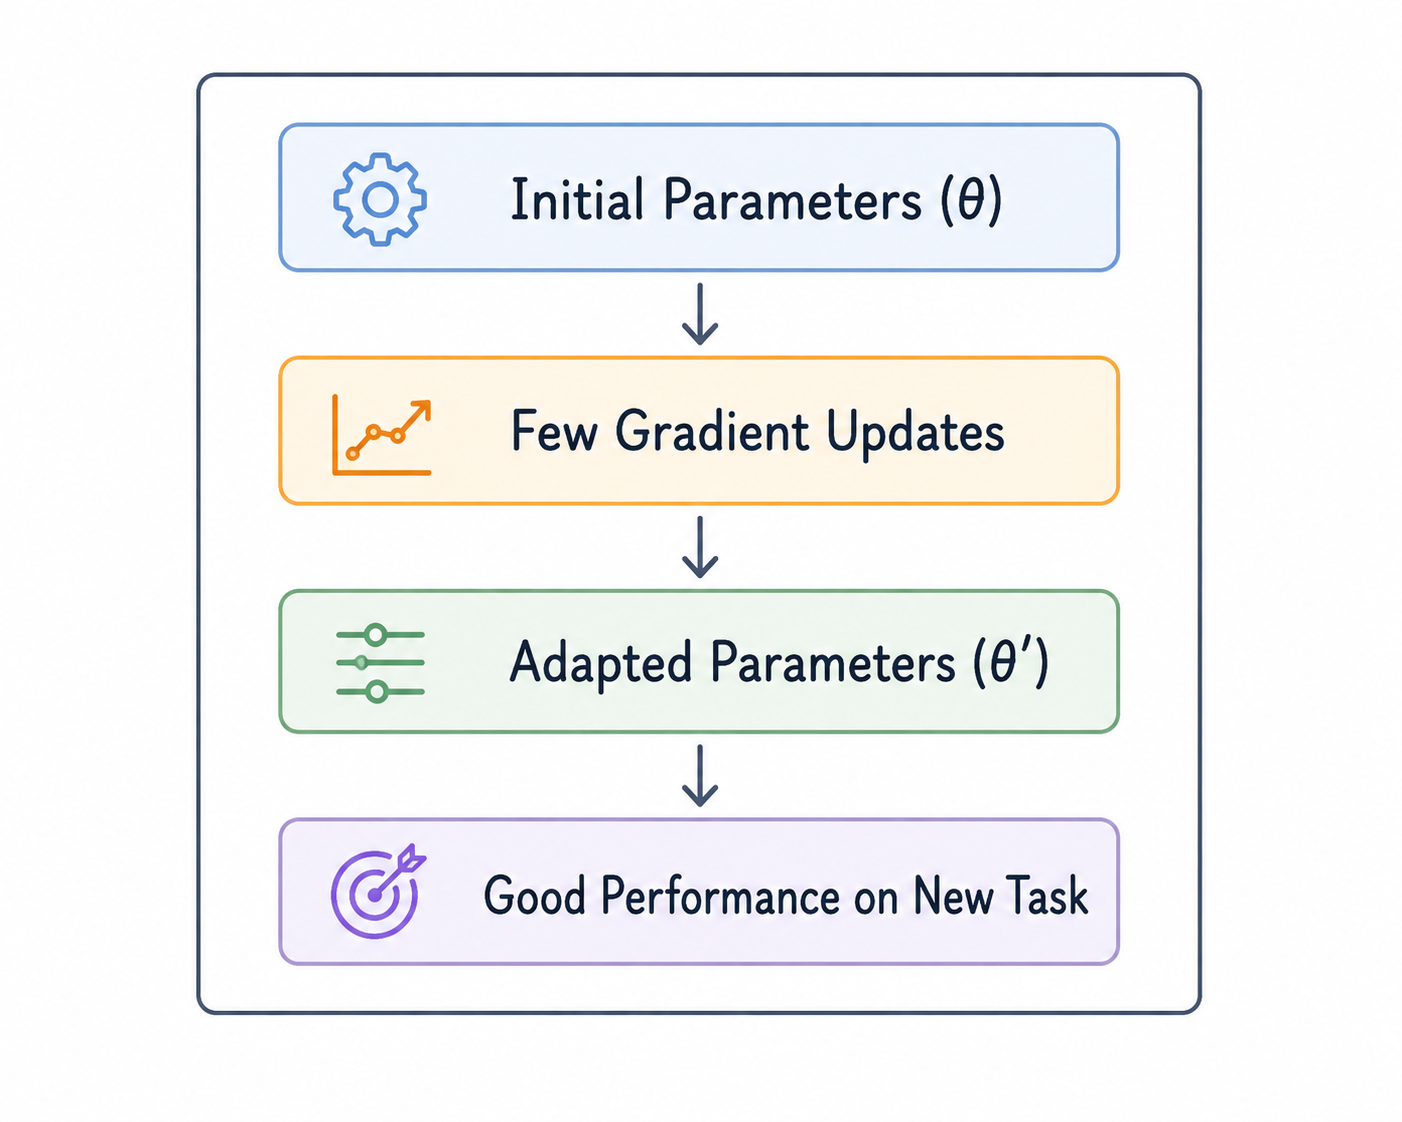
\includegraphics[width=0.95\textwidth]{figures/11-15 figure.png}
\end{figure}

\subsubsection*{The Two Loops of MAML}

MAML operates using two nested optimization loops:

\textbf{1. Inner Loop (Task Adaptation)}:
\begin{itemize}
    \item For each task $\mathcal{T}_i$, the model starts from the current initial parameters $\theta$.
    \item Using the task's Support Set $S_i$, it performs $1$ or a few steps of gradient descent to obtain task-specific parameters $\theta'_i$:
    \[
    \theta'_i = \theta - \alpha \nabla_\theta \mathcal{L}_{\mathcal{T}_i}(\theta)
    \]
    where $\alpha$ is the inner-loop learning rate.
\end{itemize}

\textbf{2. Outer Loop (Meta-Update)}:
\begin{itemize}
    \item The adapted parameters $\theta'_i$ are evaluated on the Query Set $Q_i$ of each task to compute the meta-loss:
    \[
    \mathcal{L}_{\text{meta}}(\theta) = \sum_{\mathcal{T}_i} \mathcal{L}_{\mathcal{T}_i}(\theta'_i)
    \]
    \item The initial parameters $\theta$ are updated using the meta-gradient calculated across all tasks:
    \[
    \theta \leftarrow \theta - \beta \nabla_\theta \sum_{\mathcal{T}_i} \mathcal{L}_{\mathcal{T}_i}(\theta'_i)
    \]
    where $\beta$ is the outer-loop learning rate.
\end{itemize}

\begin{figure}[H]
\centering
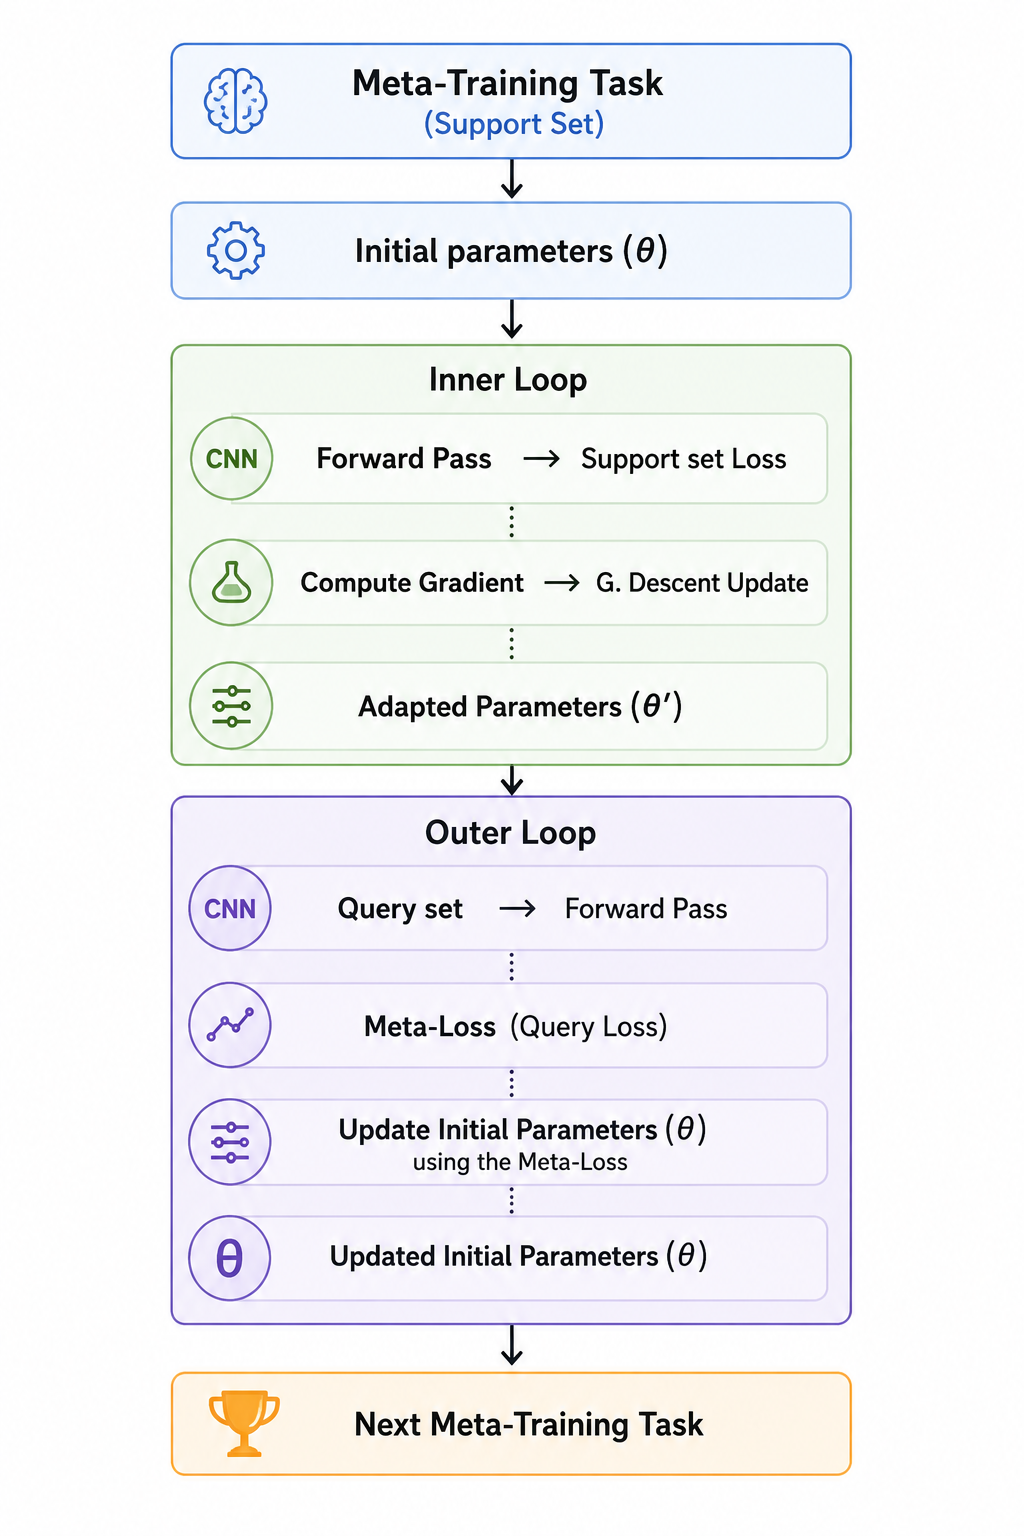
\includegraphics[width=0.95\textwidth]{figures/11-16 figure.png}
\caption{First-Order MAML (FOMAML) Pipeline and Parameter Update Approximation.}
\label{fig:fomaml_pipeline}
\end{figure}

\vspace{0.5cm}
\noindent\rule{\textwidth}{0.4pt}
\vspace{0.5cm}


MAML learns an initial set of parameters $\theta$ that acts as a universal starting point for many different tasks. Instead of optimizing the model for one specific task, MAML optimizes the initialization itself so that the model can adapt to a new task with only a few gradient updates.

\begin{figure}[H]
\centering
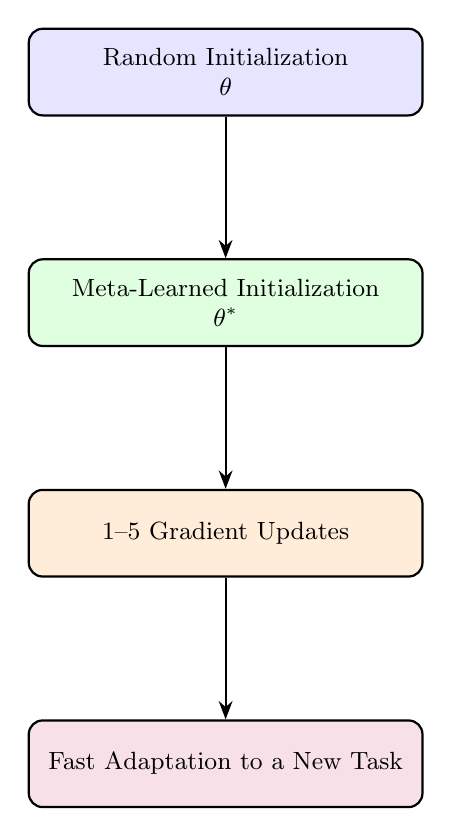
\begin{tikzpicture}[
    node distance=1.8cm,
    every node/.style={font=\small},
    block/.style={
        draw,
        rounded corners=5pt,
        thick,
        minimum width=5cm,
        minimum height=1.1cm,
        align=center,
        fill=blue!10
    },
    arrow/.style={
        ->,
        thick,
        >=Stealth
    }
]

\node[block] (random)
{Random Initialization\\$\theta$};

\node[block, below=of random, fill=green!12] (meta)
{Meta-Learned Initialization\\$\theta^\ast$};

\node[block, below=of meta, fill=orange!15] (adapt)
{1--5 Gradient Updates};

\node[block, below=of adapt, fill=purple!12] (task)
{Fast Adaptation to a New Task};

\draw[arrow] (random) -- (meta);
\draw[arrow] (meta) -- (adapt);
\draw[arrow] (adapt) -- (task);

\end{tikzpicture}
\caption{MAML learns a parameter initialization that can rapidly adapt to unseen tasks with only a few gradient updates.}
\end{figure}

After being trained on thousands of different tasks, the learned initialization converges to a region of the parameter space from which most unseen tasks can be solved with only $1$--$5$ gradient updates. Rather than memorizing previous tasks, MAML learns a parameter initialization that enables rapid adaptation to new tasks.
\subsection*{Model-Agnostic Meta-Learning (MAML)}
MAML is model-agnostic, meaning it is not tied to a specific neural network architecture. It can be applied to any model that is trainable using gradient descent. Example: CNN, ResNet, ViT, Transformer, LSTM, MLP.

The only requirement is that the model's parameters can be updated through gradient-based optimization.

This flexibility is the reason behind the name \textbf{Model-Agnostic Meta-Learning (MAML)}.

\subsection*{Advantages and Limitations}

\textbf{Advantages}:
\begin{itemize}
    \item Learns parameters that adapt very quickly.
    \item Works with almost any neural network architecture.
    \item Applicable beyond classification (regression, reinforcement learning...).
\end{itemize}

\textbf{Limitations}:
\begin{enumerate}
    \item \textbf{Computationally Expensive}: Each task requires:
    \begin{itemize}
        \item Forward pass
        \item Backward pass (inner loop)
        \item Another forward/backward pass (outer loop)
    \end{itemize}
    Training is much slower than standard supervised learning.

    \item \textbf{High Memory Usage}: The outer loop needs gradients through the inner optimization steps. This means storing additional computation graphs in memory.

    \item \textbf{Second-Order Derivative}: The original MAML algorithm computes gradients of gradients (second-order derivative). These are mathematically correct but computationally expensive.
\end{enumerate}

This limitation directly motivated the next algorithm: \textbf{First-Order MAML (FOMAML)}.

\section{Why Does MAML Need Second-Order Derivatives?}

For each meta-learning task, MAML performs two optimization stages:
\begin{center}
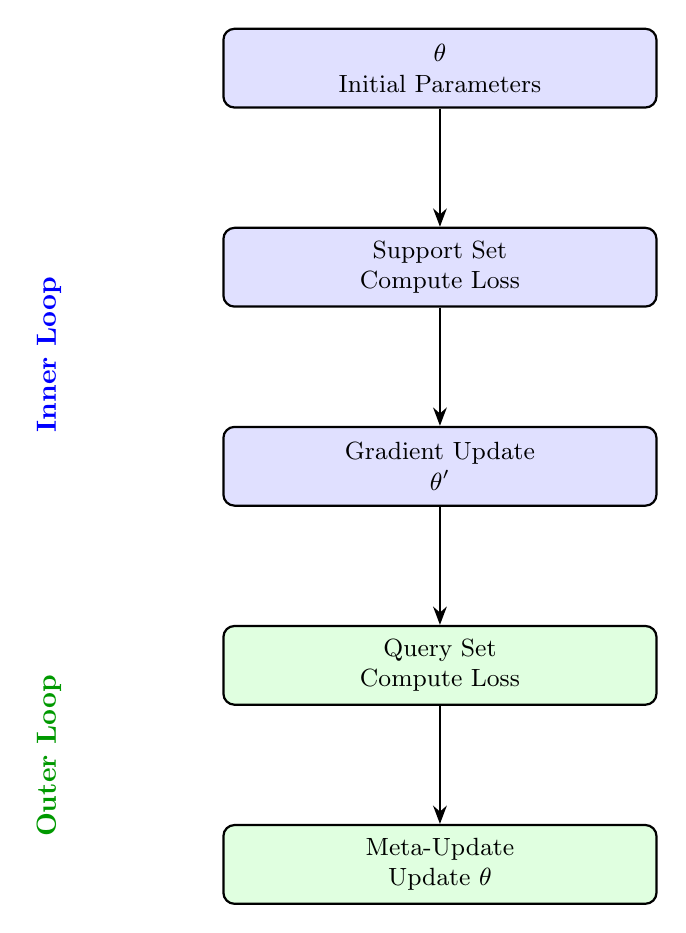
\begin{tikzpicture}[
every node/.style={font=\small},
block/.style={
draw,
rounded corners=4pt,
minimum width=5.5cm,
minimum height=1cm,
align=center,
thick
},
inner/.style={block,fill=blue!12},
outer/.style={block,fill=green!12},
arrow/.style={->,>=Stealth,thick}
]

% Nodes
\node[inner] (theta)
{$\theta$\\Initial Parameters};

\node[inner, below=1.5cm of theta] (support)
{Support Set\\Compute Loss};

\node[inner, below=1.5cm of support] (update)
{Gradient Update\\$\theta'$};

\node[outer, below=1.5cm of update] (query)
{Query Set\\Compute Loss};

\node[outer, below=1.5cm of query] (meta)
{Meta-Update\\Update $\theta$};

% Arrows
\draw[arrow] (theta) -- (support);
\draw[arrow] (support) -- (update);
\draw[arrow] (update) -- (query);
\draw[arrow] (query) -- (meta);

% Labels
\node[left=2.2cm of support,
font=\bfseries\color{blue},rotate=90]
{Inner Loop};

\node[left=2.2cm of query,
font=\bfseries\color{green!60!black},rotate=90]
{Outer Loop};

\end{tikzpicture}
\end{center}
The objective of the inner loop is to adapt the model to the current task using the Support Set, while the outer loop evaluates the adapted model on the Query Set and updates the initial parameters so that future adaptation becomes faster.
\subsection*{Inner Update}

The adapted parameters are obtained by performing one gradient descent step on the Support Set:

\[
\theta'
=
\theta
-
\alpha
\nabla_{\theta}
\mathcal{L}_{\text{support}}(\theta)
\]

Since the updated parameters $\theta'$ are computed directly from $\theta$, they are not independent. Instead,

\[
\theta' = f(\theta),
\]

which implies

\[
\frac{\partial \theta'}{\partial \theta}\neq0.
\]
\subsection*{Meta-Loss}

After adaptation, the updated model is evaluated on the Query Set:

\[
\mathcal{L}_{\text{meta}}
=
\mathcal{L}_{\text{query}}(\theta').
\]

Although the Meta-Loss is evaluated using $\theta'$, the adapted parameters themselves depend on the original initialization $\theta$. Consequently, the Meta-Loss is also an indirect function of $\theta$.
\subsection*{Backpropagating Through the Inner Update}

To optimize the initial parameters, MAML must differentiate through the gradient update itself.

Using the chain rule,

\[
\boxed{
\frac{\partial \mathcal{L}_{\text{meta}}}{\partial \theta}
=
\frac{\partial \mathcal{L}_{\text{meta}}}{\partial \theta'}
\cdot
\frac{\partial \theta'}{\partial \theta}
}
\]

where

\[
\frac{\partial \theta'}{\partial \theta}
=
I
-
\alpha
\frac{\partial^2
\mathcal{L}_{\text{support}}}
{\partial\theta^2}.
\]

The second derivative (the Hessian) appears because the gradient update itself depends on the gradient of the Support Loss.
\begin{center}
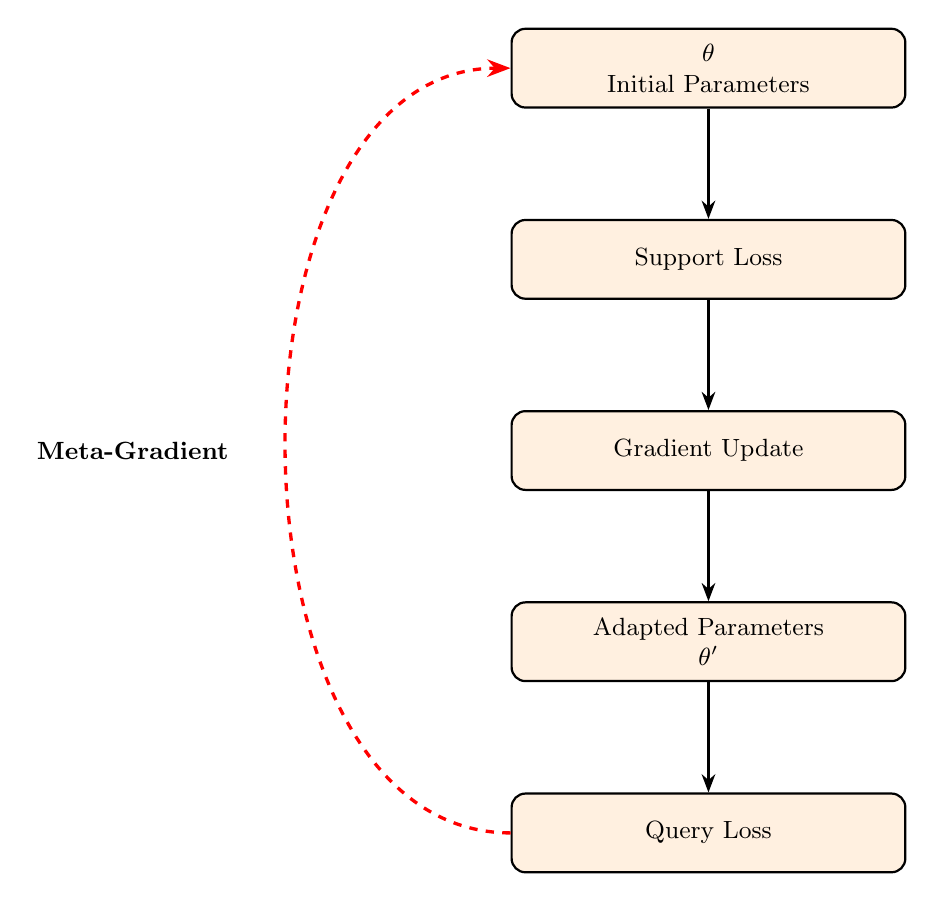
\begin{tikzpicture}[
    every node/.style={font=\small},
    block/.style={
        draw,
        rounded corners=5pt,
        minimum width=5cm,
        minimum height=1cm,
        align=center,
        fill=orange!12,
        thick
    },
    arrow/.style={
        ->,
        >=Stealth,
        thick
    },
    back/.style={
        ->,
        >=Stealth,
        dashed,
        red,
        very thick
    }
]

% Forward pass
\node[block] (theta)
{$\theta$\\Initial Parameters};

\node[block, below=1.4cm of theta] (loss1)
{Support Loss};

\node[block, below=1.4cm of loss1] (grad)
{Gradient Update};

\node[block, below=1.4cm of grad] (theta2)
{Adapted Parameters\\$\theta'$};

\node[block, below=1.4cm of theta2]
(loss2) {Query Loss};

% Forward arrows
\draw[arrow] (theta) -- (loss1);
\draw[arrow] (loss1) -- (grad);
\draw[arrow] (grad) -- (theta2);
\draw[arrow] (theta2) -- (loss2);

% Backward (Meta-Gradient)
\draw[back]
(loss2.west)
to[out=180,in=180]
node[left=0.6cm, align=center]
{\textbf{Meta-Gradient}}
(theta.west);

\end{tikzpicture}
\end{center}
\section{First-Order Model-Agnostic Meta-Learning (FOMAML)}

Although MAML achieves strong few-shot learning performance, its main limitation is the computational cost associated with second-order derivatives. During each meta-update, MAML must backpropagate through the inner optimization step, which requires:

\begin{itemize}
    \item computing second-order derivatives (Hessian-related terms);
    \item storing the complete computation graph for the inner update;
    \item increased GPU memory consumption;
    \item longer training time.
\end{itemize}

To address these limitations, researchers proposed \textbf{First-Order Model-Agnostic Meta-Learning (FOMAML)}, a computationally efficient variant of MAML that removes the need for second-order derivatives while preserving the same meta-learning framework.

The key idea behind FOMAML is that the adapted parameters $\theta'$ are typically very close to the initial parameters $\theta$. Therefore, the dependence of $\theta'$ on $\theta$ is ignored during the computation of the meta-gradient.

\subsection*{First-Order Approximation}

Recall that the exact MAML meta-gradient is

\[
\frac{\partial \mathcal{L}_{\text{meta}}}{\partial \theta}
=
\frac{\partial \mathcal{L}_{\text{meta}}}{\partial \theta'}
\cdot
\frac{\partial \theta'}{\partial \theta}.
\]

FOMAML approximates the Jacobian of the inner update by the identity matrix,

\[
\frac{\partial \theta'}{\partial \theta}
\approx
I,
\]

where $I$ denotes the identity matrix.

Consequently, the meta-gradient simplifies to

\[
\boxed{
\frac{\partial \mathcal{L}_{\text{meta}}}{\partial \theta}
\approx
\frac{\partial \mathcal{L}_{\text{meta}}}{\partial \theta'}
}
\]

This approximation eliminates the computation of Hessian terms, allowing gradients to be computed using only first-order information.

\vspace{0.5cm}

\begin{figure}[H]
\centering
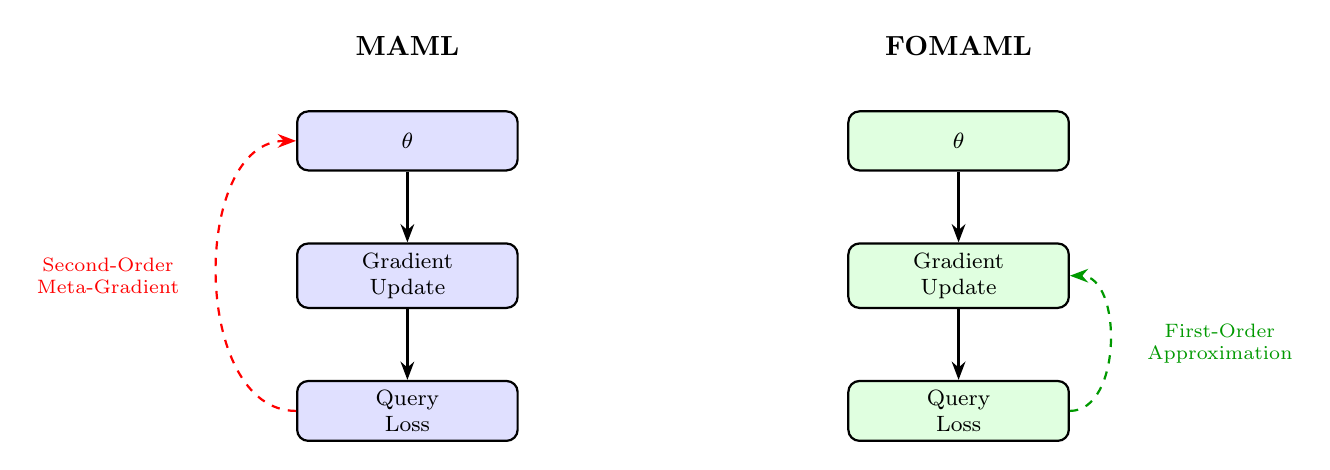
\begin{tikzpicture}[
every node/.style={font=\footnotesize},
block/.style={
draw,
rounded corners=4pt,
minimum width=2.8cm,
minimum height=0.75cm,
align=center,
thick
},
maml/.style={block,fill=blue!12},
fomaml/.style={block,fill=green!12},
arrow/.style={->,>=Stealth,thick},
back1/.style={->,>=Stealth,dashed,red,thick},
back2/.style={->,>=Stealth,dashed,green!60!black,thick}
]

%%%%%%%%%%%%%%%%%%%%%
% MAML
%%%%%%%%%%%%%%%%%%%%%

\node[font=\bfseries] at (-3.5,1.2) {MAML};

\node[maml] (mtheta) at (-3.5,0)
{$\theta$};

\node[maml,below=0.9cm of mtheta] (mupdate)
{Gradient\\Update};

\node[maml,below=0.9cm of mupdate] (mloss)
{Query\\Loss};

\draw[arrow] (mtheta)--(mupdate);
\draw[arrow] (mupdate)--(mloss);

\draw[back1]
(mloss.west)
to[out=180,in=180]
node[left=0.35cm,font=\scriptsize,align=center]
{Second-Order\\Meta-Gradient}
(mtheta.west);

%%%%%%%%%%%%%%%%%%%%%
% FOMAML
%%%%%%%%%%%%%%%%%%%%%

\node[font=\bfseries] at (3.5,1.2) {FOMAML};

\node[fomaml] (ftheta) at (3.5,0)
{$\theta$};

\node[fomaml,below=0.9cm of ftheta] (fupdate)
{Gradient\\Update};

\node[fomaml,below=0.9cm of fupdate] (floss)
{Query\\Loss};

\draw[arrow] (ftheta)--(fupdate);
\draw[arrow] (fupdate)--(floss);

\draw[back2]
(floss.east)
to[out=0,in=0]
node[right=0.35cm,font=\scriptsize,align=center]
{First-Order\\Approximation}
(fupdate.east);

\end{tikzpicture}
\caption{Comparison between MAML and FOMAML. MAML computes second-order meta-gradients by differentiating through the inner update, whereas FOMAML ignores this dependency and uses a first-order approximation.}
\end{figure}



\subsection*{Why Does This Approximation Work?}

During the inner loop, the model performs only a small number of gradient updates (typically 1--5), resulting in relatively small changes to the parameters:

\[
\theta
\longrightarrow
\text{Small Gradient Update}
\longrightarrow
\theta'.
\]

Since $\theta'$ remains close to $\theta$, treating the two parameter sets as approximately equivalent introduces only a small approximation error while substantially reducing computational complexity.

\subsection*{Advantages}

Compared with MAML, FOMAML offers several practical benefits:

\begin{itemize}
    \item significantly lower memory consumption;
    \item faster meta-training;
    \item simpler implementation because no second-order derivatives are required;
    \item performance comparable to MAML on many few-shot learning benchmarks.
\end{itemize}

\subsection*{Limitations}

Despite its computational efficiency, FOMAML remains an approximation of the original MAML algorithm. Consequently,

\begin{itemize}
    \item the computed meta-gradient is not exact;
    \item performance may degrade when the inner-loop updates produce large changes in the model parameters.
\end{itemize}
\section{Reptile}

Although FOMAML eliminates second-order derivatives, it still requires computing a meta-gradient. This raises an important question:

\begin{quote}
\emph{Can meta-learning be achieved without computing a meta-gradient at all?}
\end{quote}

This idea led to \textbf{Reptile}, proposed by OpenAI in 2018.

Reptile is an optimization-based meta-learning algorithm that completely removes the meta-gradient computation. Instead of optimizing the Query Loss as in MAML, Reptile learns a good initialization by repeatedly moving the model parameters toward task-specific solutions obtained after training on individual tasks.

Unlike MAML, Reptile does not explicitly separate each task into a Support Set and a Query Set during the meta-update. Instead, each sampled task is treated as a standard supervised learning problem, and the adapted parameters are used directly to update the initialization.
\subsection*{Training Pipeline}

For each sampled task, Reptile performs the following steps:

\begin{enumerate}
\item Initialize the model with the current parameters $\theta$.
\item Train on the sampled task for a few gradient updates to obtain adapted parameters $\theta'$.
\item Move the initialization slightly toward $\theta'$.
\end{enumerate}
\begin{figure}[H]
\centering
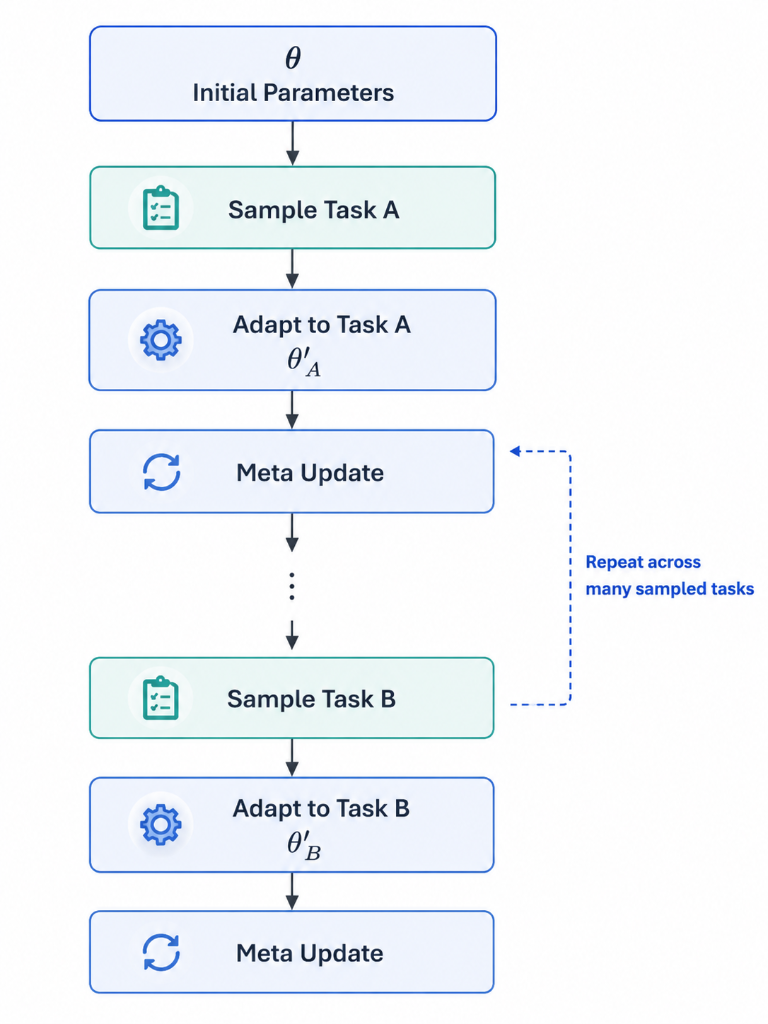
\includegraphics[width=0.55\textwidth]{figures/11-20 figure.png}
\caption{Training procedure of Reptile. For each sampled task, the model is adapted through a few gradient updates to obtain task-specific parameters. The initialization is then updated toward these adapted parameters. Repeating this process across many sampled tasks gradually learns an initialization that can rapidly adapt to unseen tasks.}
\end{figure}




After adapting to a task, Reptile updates the initialization according to

\[
\boxed{
\theta
\leftarrow
\theta
+
\epsilon
(\theta'-\theta)
}
\]

where

\begin{itemize}
\item $\theta$ is the current initialization;
\item $\theta'$ is the adapted parameter vector after training on one task;
\item $\epsilon$ is the meta-learning rate.
\end{itemize}

Rather than replacing the initialization with $\theta'$, Reptile performs only a partial update, gradually moving the initialization toward task-specific solutions.
\subsection*{Meta-Update}

After adapting to a task, Reptile updates the initialization according to

\[
\boxed{
\theta
\leftarrow
\theta
+
\epsilon
(\theta'-\theta)
}
\]

where

\begin{itemize}
\item $\theta$ is the current initialization;
\item $\theta'$ is the adapted parameter vector after training on one task;
\item $\epsilon$ is the meta-learning rate.
\end{itemize}

Rather than replacing the initialization with $\theta'$, Reptile performs only a partial update, gradually moving the initialization toward task-specific solutions.
\subsection*{Why Does Reptile Work?}

Different tasks generally have different optimal parameter values.

\[
\theta
\rightarrow
\theta_A'
\qquad
\theta
\rightarrow
\theta_B'
\qquad
\theta
\rightarrow
\theta_C'
\]

Reptile repeatedly moves the initialization toward the adapted parameters obtained from many different tasks. Over time, the initialization converges to a region of the parameter space that is close to the optima of multiple tasks.

As a result, when a new unseen task is encountered, only a few gradient updates are required to achieve good performance.
\subsection*{Advantages}

Compared with MAML and FOMAML, Reptile offers several practical advantages:

\begin{itemize}
\item no second-order derivatives;
\item no meta-gradient computation;
\item low memory consumption;
\item fast meta-training;
\item simple implementation using any standard optimizer;
\item competitive performance on many few-shot learning benchmarks.
\end{itemize}
\subsection*{Limitations}

Reptile remains an approximation of the meta-learning objective because it never explicitly optimizes the Query Loss. Consequently,

\begin{itemize}
\item it may perform slightly worse than MAML on more challenging tasks;
\item its updates are less theoretically grounded than the exact meta-gradient used by MAML.
\end{itemize}

Nevertheless, the simplicity and computational efficiency of Reptile make it an attractive choice for large-scale few-shot learning problems and resource-constrained environments.

\section{Memory-Based Meta-Learning}

The meta-learning methods presented so far can be broadly divided into two categories:

\begin{itemize}
    \item \textbf{Metric-based methods}, such as Siamese Networks, Matching Networks, Prototypical Networks, and Relation Networks, which perform adaptation by comparing learned feature representations.
    \item \textbf{Optimization-based methods}, such as MAML, FOMAML, and Reptile, which adapt the model parameters through gradient-based optimization.
\end{itemize}

Although these approaches differ in their adaptation mechanisms, they share a common characteristic: the knowledge acquired during training is primarily stored in the model parameters.

Memory-Based Meta-Learning introduces a different paradigm by equipping the model with an \textbf{external differentiable memory}. Instead of encoding all task-specific knowledge in the network weights, the model dynamically stores and retrieves information from this external memory during inference. Consequently, adaptation is achieved by updating the memory contents rather than modifying the model parameters.

One of the earliest and most influential architectures following this paradigm is the \textbf{Memory-Augmented Neural Network (MANN)}.
\begin{figure}[H]
\centering
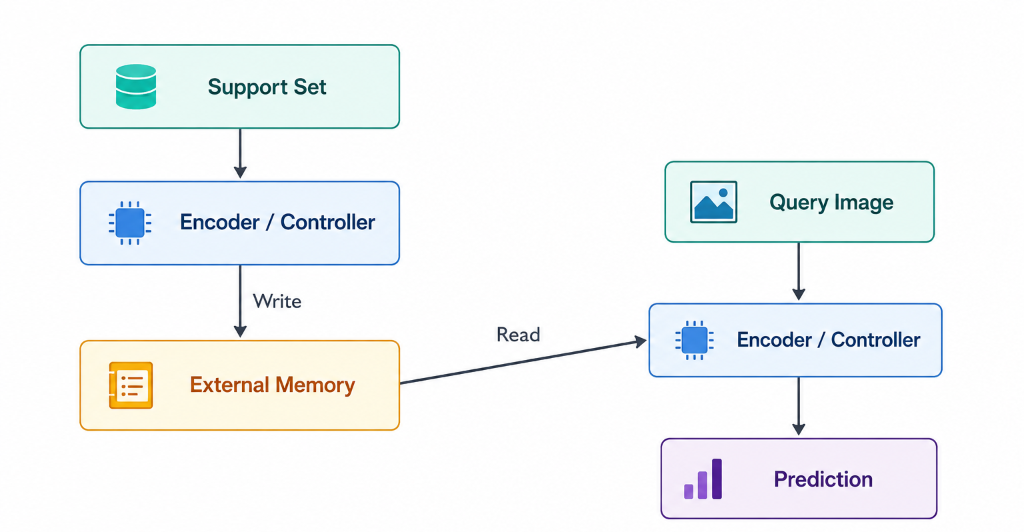
\includegraphics[width=0.85\textwidth]{figures/11-21 figure.png}
\caption{Overview of a Memory-Augmented Neural Network (MANN). Support examples are encoded and written into an external memory. During inference, the query representation retrieves relevant information from memory to produce the final prediction.}
\end{figure}
\subsection*{Architecture}
\begin{figure}[H]
\centering
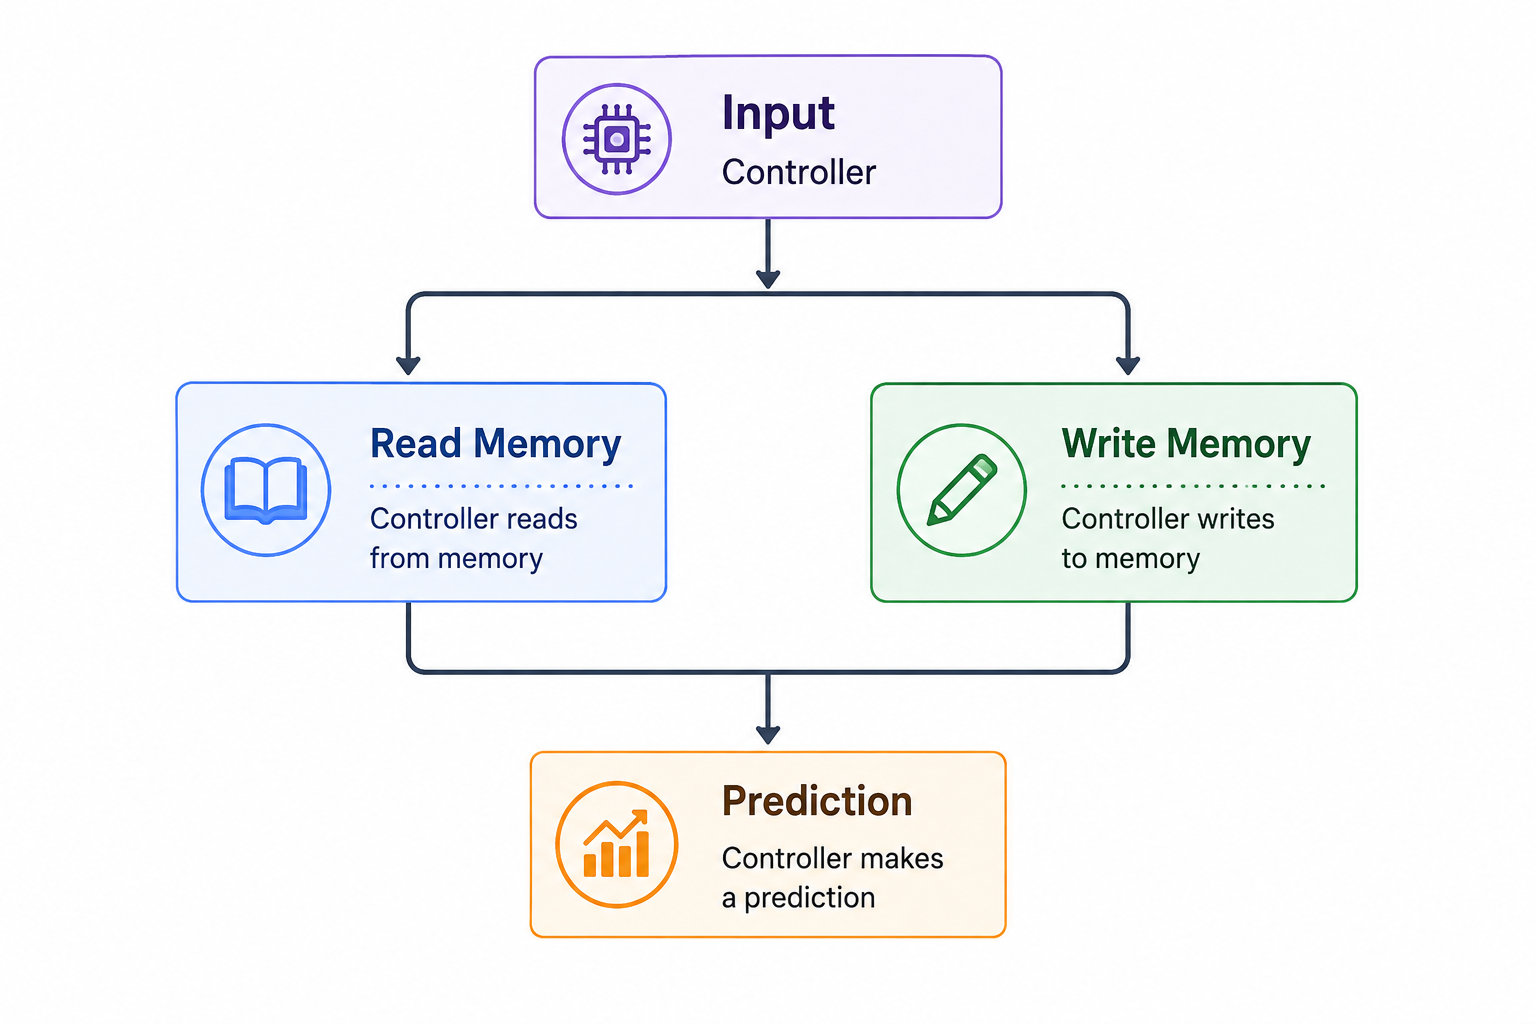
\includegraphics[width=0.95\textwidth]{figures/11-19 figure.png}
\end{figure}

A typical Memory-Augmented Neural Network consists of two main components:

\begin{enumerate}
\item A \textbf{controller}, usually implemented using an LSTM or a Transformer, responsible for interacting with the external memory.
\item An \textbf{external memory}, represented as a differentiable memory matrix that stores task-specific information.
\end{enumerate}
\subsection*{Memory Operations}

During the support phase, each support example is encoded into a feature representation. The controller writes these representations into the external memory, allowing the model to accumulate information about the current task.

During inference, the query image is encoded by the same controller. Rather than relying solely on the network weights, the controller retrieves the most relevant information from the external memory. The retrieved memory is then combined with the query representation to generate the final prediction.
\subsection*{Why Does It Work?}

Unlike optimization-based meta-learning methods, MANNs do not perform gradient updates during inference. Adaptation occurs by dynamically modifying the memory contents while keeping the model parameters fixed. This enables rapid adaptation to unseen tasks without requiring additional optimization.
\subsection*{Advantages}

\begin{itemize}
\item rapid adaptation without gradient updates;
\item dynamic storage of task-specific information;
\item efficient inference for few-shot learning;
\item well suited for sequential and online learning scenarios.
\end{itemize}

\subsection*{Limitations}

\begin{itemize}
\item limited memory capacity;
\item effective performance depends on learning appropriate read and write operations;
\item computational cost increases as the memory size grows.
\end{itemize}
\subsection*{Comparison of Meta-Learning Paradigms}


\begin{table}[H]
\centering
\caption{Comparison of the main meta-learning paradigms.}
\label{tab:meta_learning_comparison}
\renewcommand{\arraystretch}{1.3}

\renewcommand{\arraystretch}{1.35}

\begin{tabularx}{\textwidth}{
>{\bfseries}p{2.8cm}
X
p{2.9cm}
X}
\toprule

Paradigm &
Adaptation Mechanism &
Updated During Inference &
Representative Methods \\

\midrule

Metric-Based &
Similarity comparison in an embedding space &
None &
Siamese, Matching, Prototypical, Relation \\

Optimization-Based &
Gradient-based parameter adaptation &
Model weights &
MAML, FOMAML, Reptile \\

Memory-Based &
Reading from and writing to an external memory &
External memory only &
Memory-Augmented Neural Networks (MANN) \\

\bottomrule
\end{tabularx}

\end{table}

\begin{figure}[H]
\centering

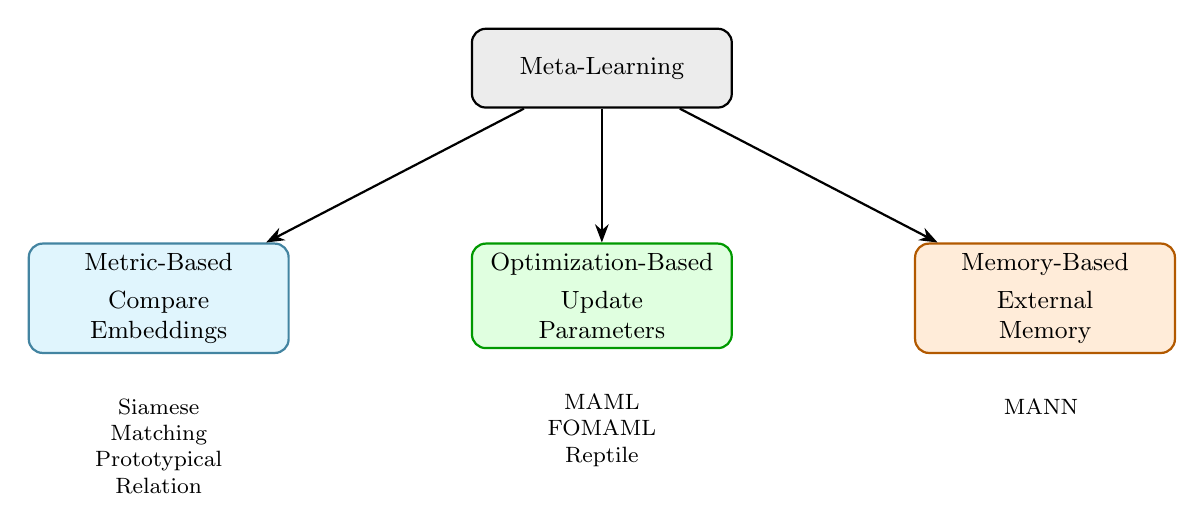
\begin{tikzpicture}[
every node/.style={font=\small},
box/.style={
draw,
rounded corners=5pt,
minimum width=3.3cm,
minimum height=1cm,
align=center,
thick
},
metric/.style={box,fill=cyan!12,draw=cyan!60!black},
optim/.style={box,fill=green!12,draw=green!60!black},
memory/.style={box,fill=orange!15,draw=orange!70!black},
main/.style={box,fill=gray!15,draw=black},
arrow/.style={->,>=Stealth,thick}
]

%%%%%%%%%%%%%%%%%%%%%%%%%%%%%%%%%%%%%%%%%%
% Main node
%%%%%%%%%%%%%%%%%%%%%%%%%%%%%%%%%%%%%%%%%%

\node[main] (meta)
{Meta-Learning};

%%%%%%%%%%%%%%%%%%%%%%%%%%%%%%%%%%%%%%%%%%
% Three categories
%%%%%%%%%%%%%%%%%%%%%%%%%%%%%%%%%%%%%%%%%%

\node[metric,below left=1.7cm and 2.3cm of meta]
(metric)
{Metric-Based\\[1mm]
Compare\\Embeddings};

\node[optim,below=1.7cm of meta]
(optim)
{Optimization-Based\\[1mm]
Update\\Parameters};

\node[memory,below right=1.7cm and 2.3cm of meta]
(memory)
{Memory-Based\\[1mm]
External\\Memory};

%%%%%%%%%%%%%%%%%%%%%%%%%%%%%%%%%%%%%%%%%%
% Connections
%%%%%%%%%%%%%%%%%%%%%%%%%%%%%%%%%%%%%%%%%%

\draw[arrow] (meta)--(metric);
\draw[arrow] (meta)--(optim);
\draw[arrow] (meta)--(memory);

%%%%%%%%%%%%%%%%%%%%%%%%%%%%%%%%%%%%%%%%%%
% Representative methods
%%%%%%%%%%%%%%%%%%%%%%%%%%%%%%%%%%%%%%%%%%

\node[align=center,font=\footnotesize,below=0.45cm of metric]
{
Siamese\\
Matching\\
Prototypical\\
Relation
};

\node[align=center,font=\footnotesize,below=0.45cm of optim]
{
MAML\\
FOMAML\\
Reptile
};

\node[align=center,font=\footnotesize,below=0.45cm of memory]
{
MANN
};

\end{tikzpicture}



\end{figure}
\clearpage
\section{When to Use (Transfer Learning vs. Meta-Learning)}

Although both Transfer Learning and Meta-Learning aim to adapt pretrained models to new tasks, they are designed for different scenarios. The choice between them mainly depends on the amount of available labeled data and the expected deployment setting.

Transfer Learning is most effective when a moderate or large labeled dataset is available for the target task. In contrast, Meta-Learning is specifically designed for situations where only a few labeled examples are available and rapid adaptation to new tasks is required.

\begin{table}[H]
\centering

\renewcommand{\arraystretch}{1.3}

\begin{tabular}{|p{7cm}|p{5cm}|}
\hline
\textbf{Scenario} & \textbf{Recommended Approach} \\
\hline
Large labeled dataset available & Transfer Learning \\
\hline
Moderate number of labeled examples & Transfer Learning \\
\hline
Only 1--10 labeled examples per class & Meta-Learning \\
\hline
New tasks appear frequently & Meta-Learning \\
\hline
Fixed downstream task & Transfer Learning \\
\hline
Rapid adaptation to unseen tasks & Meta-Learning \\
\hline
\end{tabular}
\caption{Comparison of scenarios where Transfer Learning and Meta-Learning are most appropriate.}
\label{tab:transfer_vs_meta}
\end{table}

\subsection*{Combining Transfer Learning and Meta-Learning}

Rather than viewing Transfer Learning and Meta-Learning as competing approaches, modern few-shot learning systems often combine both techniques to exploit their complementary strengths.

Transfer Learning first learns a rich and general feature representation from a large-scale dataset, while Meta-Learning subsequently teaches the model how to adapt these representations rapidly to new tasks using only a few training examples.

The overall process can be summarized as follows:
\begin{figure}[H]
\centering
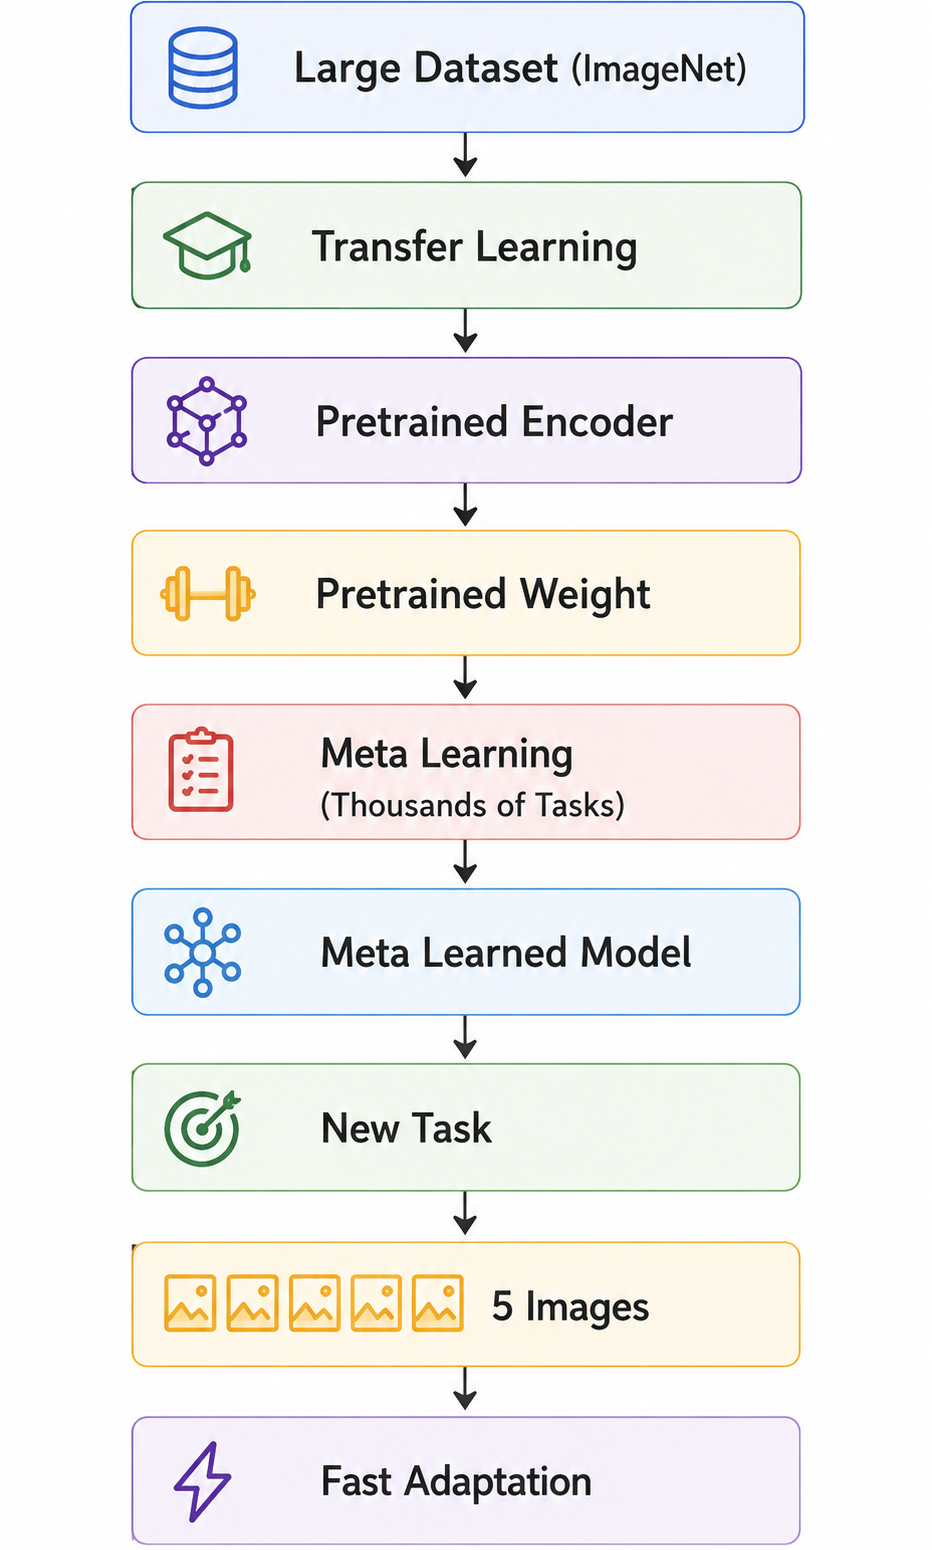
\includegraphics[width=0.95\textwidth]{figures/11-25 figure.png}
\label{fig:peft_transition}
\end{figure}

During the transfer learning stage, the backbone network learns general visual representations from a large dataset such as ImageNet. These representations capture universal image characteristics, including

\begin{itemize}
    \item edges;
    \item textures;
    \item shapes;
    \item object parts;
    \item high-level semantic concepts.
\end{itemize}

Although these pretrained features are highly informative, they are not specifically optimized for rapid adaptation to unseen tasks.

In the second stage, Meta-Learning uses the pretrained weights as the initialization for meta-training. Rather than learning visual features from scratch, the model learns how to efficiently adapt these already powerful representations to new tasks with only a few labeled examples.

By combining Transfer Learning with Meta-Learning, the resulting model benefits from both strong feature extraction and rapid adaptation, making this strategy one of the most effective approaches for modern few-shot learning systems.




\chapter{Parameter-efficient Fine-Tuning (PEFT)}





\section{Modern LLM Fine-Tuning}

Recent years have witnessed an unprecedented growth in the size of Large Language Models (LLMs). Early neural language models contained only millions of parameters, whereas modern foundation models contain billions or even hundreds of billions of parameters. These models acquire extensive knowledge during large-scale pretraining, enabling them to perform a wide range of downstream tasks such as question answering, summarization, translation, reasoning, and code generation.

However, pretrained LLMs are general-purpose models. To specialize an LLM for a particular application (e.g., medicine, finance, or law), it must be adapted using task-specific data. Traditionally, this adaptation is achieved through \textbf{full fine-tuning}, in which every trainable parameter of the pretrained model is updated.
\subsection*{Why Can't We Fully Fine-Tune Large LLMs?}

The traditional fine-tuning pipeline is illustrated below:

\[
\text{Pretraining}
\longrightarrow
\text{Pretrained Model}
\longrightarrow
\text{Full Fine-Tuning}
\longrightarrow
\text{Task-Specific Model}
\]

During full fine-tuning, gradients are computed for every trainable layer, and every parameter of the model is updated using the downstream dataset.

For relatively small neural networks, updating all parameters is computationally feasible. However, modern LLMs contain billions of parameters, making full fine-tuning increasingly expensive in terms of both memory consumption and computational cost.
\begin{table}[H]
\centering
\caption{Parameter scale of representative modern Large Language Models.}
\label{tab:llm_parameters}

\renewcommand{\arraystretch}{1.25}

\begin{tabular}{lc}
\toprule
\textbf{Model} & \textbf{Parameters} \\
\midrule
Llama 3 8B  & 8 Billion \\
Llama 3 70B & 70 Billion \\
Qwen 72B    & 72 Billion \\
\bottomrule
\end{tabular}

\end{table}
Updating billions of parameters during every training step is fundamentally different from training conventional neural networks.

Training such large models requires substantially more GPU memory than simply storing the model weights. During optimization, additional information must also be maintained, including:

\begin{itemize}
    \item Model parameters;
    \item Gradients;
    \item Optimizer states;
    \item Intermediate activations.
\end{itemize}

Consequently, memory consumption grows rapidly as the number of trainable parameters increases.

Most modern LLMs are optimized using the AdamW optimizer. Unlike standard stochastic gradient descent, AdamW maintains additional statistics for every trainable parameter:

\begin{itemize}
    \item Parameter value;
    \item First moment estimate ($m$);
    \item Second moment estimate ($v$).
\end{itemize}

Therefore, each trainable parameter requires considerably more memory than its weight alone.
In addition to memory consumption, full fine-tuning is computationally expensive because every optimization step must perform

\[
\text{Forward Pass}
\longrightarrow
\text{Backward Pass}
\longrightarrow
\text{Parameter Update}
\]

for billions of trainable parameters.

As model size increases, training becomes progressively slower and requires increasingly powerful hardware.

\subsection*{Do We Really Need to Update Everything?}

Although modern LLMs already possess extensive knowledge acquired during pretraining, full fine-tuning updates every parameter regardless of whether that knowledge is relevant to the downstream task.

For example, when adapting an LLM into a medical assistant, much of its existing linguistic ability, reasoning capability, and general world knowledge remains useful. Only a relatively small amount of new task-specific knowledge must be learned.

This observation raises an important question:

\begin{center}
\emph{Is it really necessary to update billions of parameters to learn a new task?}
\end{center}

The answer is often \textbf{no}. Instead of modifying the entire model, it is possible to freeze the pretrained model and train only a small number of additional parameters while preserving the knowledge acquired during pretraining.

This idea forms the foundation of \textbf{Parameter-Efficient Fine-Tuning (PEFT)}, which dramatically reduces memory usage and computational cost while maintaining competitive performance.
\clearpage
\section{Parameter-Efficient Fine-Tuning (PEFT)}

Parameter-Efficient Fine-Tuning (PEFT) is not a single algorithm but rather a family of fine-tuning methods that share the same fundamental philosophy. Instead of updating every parameter of a pretrained Large Language Model, PEFT freezes the original model and trains only a small number of additional parameters.

The two core principles of PEFT are:

\begin{itemize}
    \item \textbf{Freeze the pretrained model:} The original LLM remains unchanged throughout training, preserving the knowledge acquired during large-scale pretraining.
    \item \textbf{Train a small set of additional parameters:} Only lightweight modules are optimized to learn the task-specific adaptation.
\end{itemize}

Conceptually, the pretrained model provides the general knowledge required for language understanding and reasoning, while the newly introduced trainable parameters learn how to adapt that knowledge to a particular downstream task.

\begin{figure}[H]
\centering
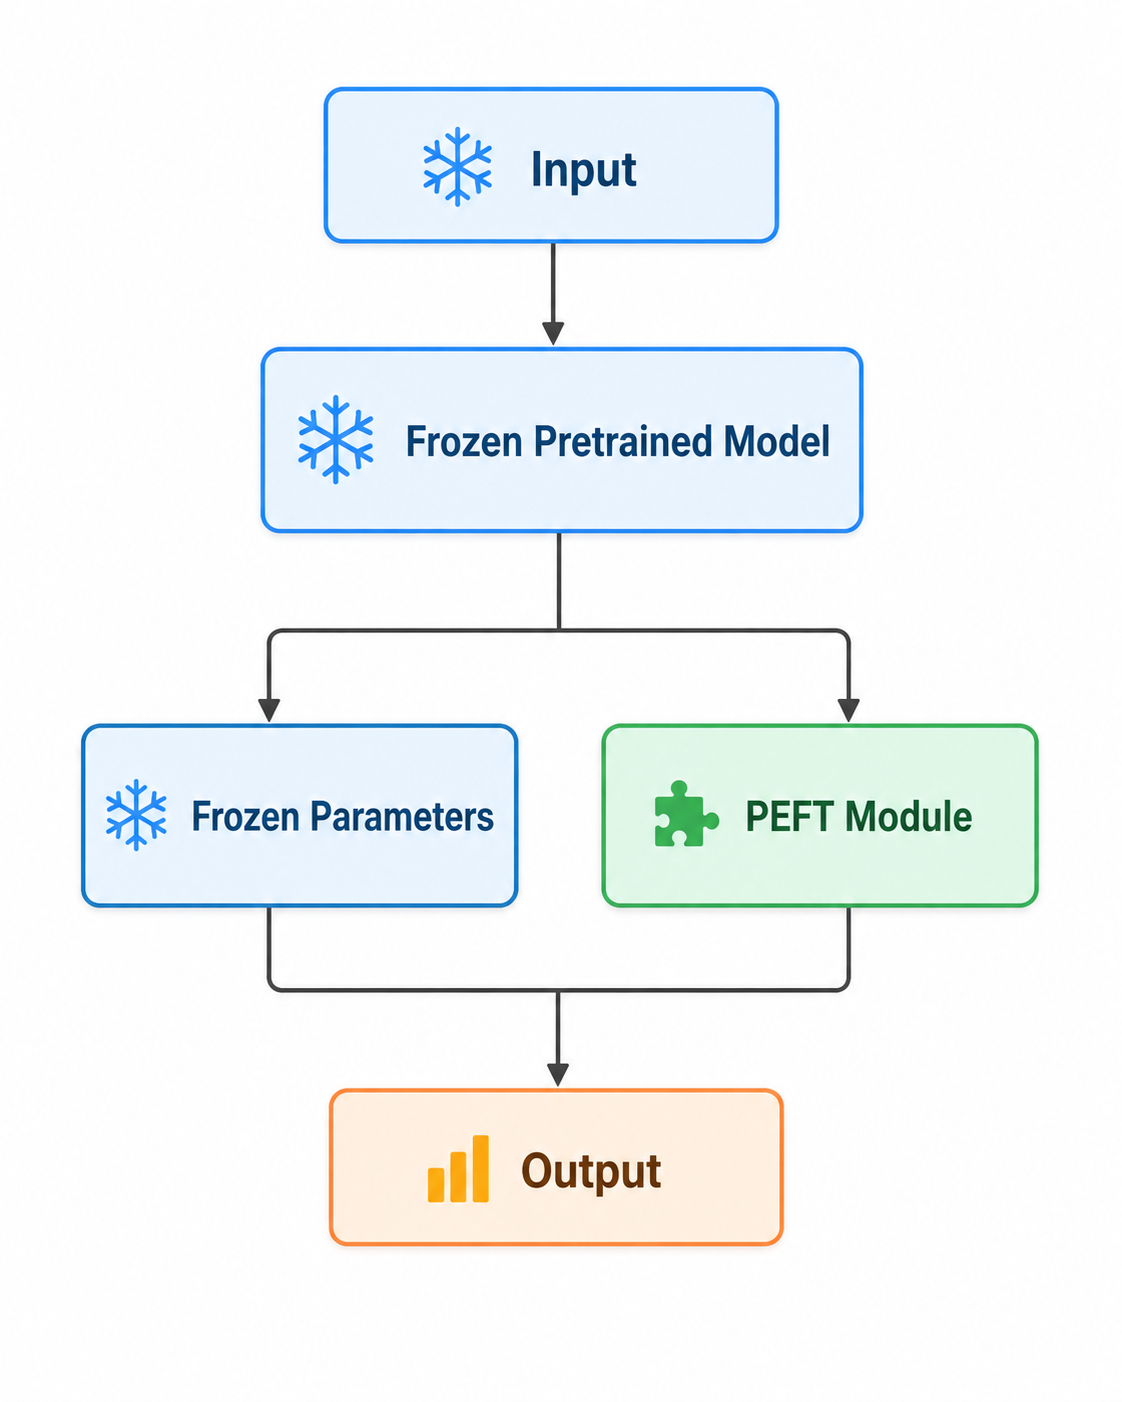
\includegraphics[width=0.95\textwidth]{figures/12-1 figure.png}
\label{fig:peft_transition_ch12}
\end{figure}

Rather than replacing the pretrained knowledge, the trainable module complements it by learning only the additional information required for the target task. Consequently, PEFT significantly reduces the number of trainable parameters, GPU memory consumption, and training time while achieving performance that is often comparable to full fine-tuning.

\section{Main PEFT Methods}

Before the introduction of LoRA, several Parameter-Efficient Fine-Tuning (PEFT) techniques had already been proposed to reduce the number of trainable parameters while preserving the knowledge contained in pretrained Large Language Models. Although these methods differ in their implementation, they all share the same objective: to adapt a frozen pretrained model by training only a small set of additional parameters.

The most representative approaches are Adapter Tuning, Prompt Tuning, and Prefix Tuning.
\subsection*{Adapter Tuning}

Adapter Tuning introduces small trainable neural networks, called \emph{adapters}, into each Transformer layer. During fine-tuning, the original model parameters remain frozen, and only the adapter modules are optimized.

A typical adapter consists of a bottleneck multilayer perceptron (MLP). The hidden representation is first projected into a lower-dimensional space and then projected back to its original dimension. For example,

\[
4096
\longrightarrow
64
\longrightarrow
4096
\]

This bottleneck architecture greatly reduces the number of trainable parameters while allowing the model to learn task-specific representations.

The overall computation can be summarized as

\[
\text{Transformer Layer}
\longrightarrow
\text{Adapter}
\longrightarrow
\text{Transformer Layer}.
\]

Because only the adapter parameters are updated, Adapter Tuning significantly reduces GPU memory consumption compared with full fine-tuning.
\subsection*{Prompt Tuning}

Prompt Tuning follows a different strategy. Instead of inserting additional neural network layers, it keeps the entire pretrained model frozen and learns only a small number of trainable embedding vectors called \emph{soft prompts}.

Consider the input sentence

\[
\texttt{Translate to French: Hello}
\]

Normally, each token is converted into an embedding vector before entering the Transformer.

Prompt Tuning prepends several trainable vectors to the input sequence:

\[
P_1,\;
P_2,\;
P_3,\;
e_1,\;
e_2,\;
e_3,\;
e_4,\;
e_5
\]

where

\begin{itemize}
\item $P_1,P_2,P_3$ are trainable prompt embeddings;
\item $e_1,\ldots,e_5$ are the original token embeddings.
\end{itemize}
\begin{figure}[H]
\centering
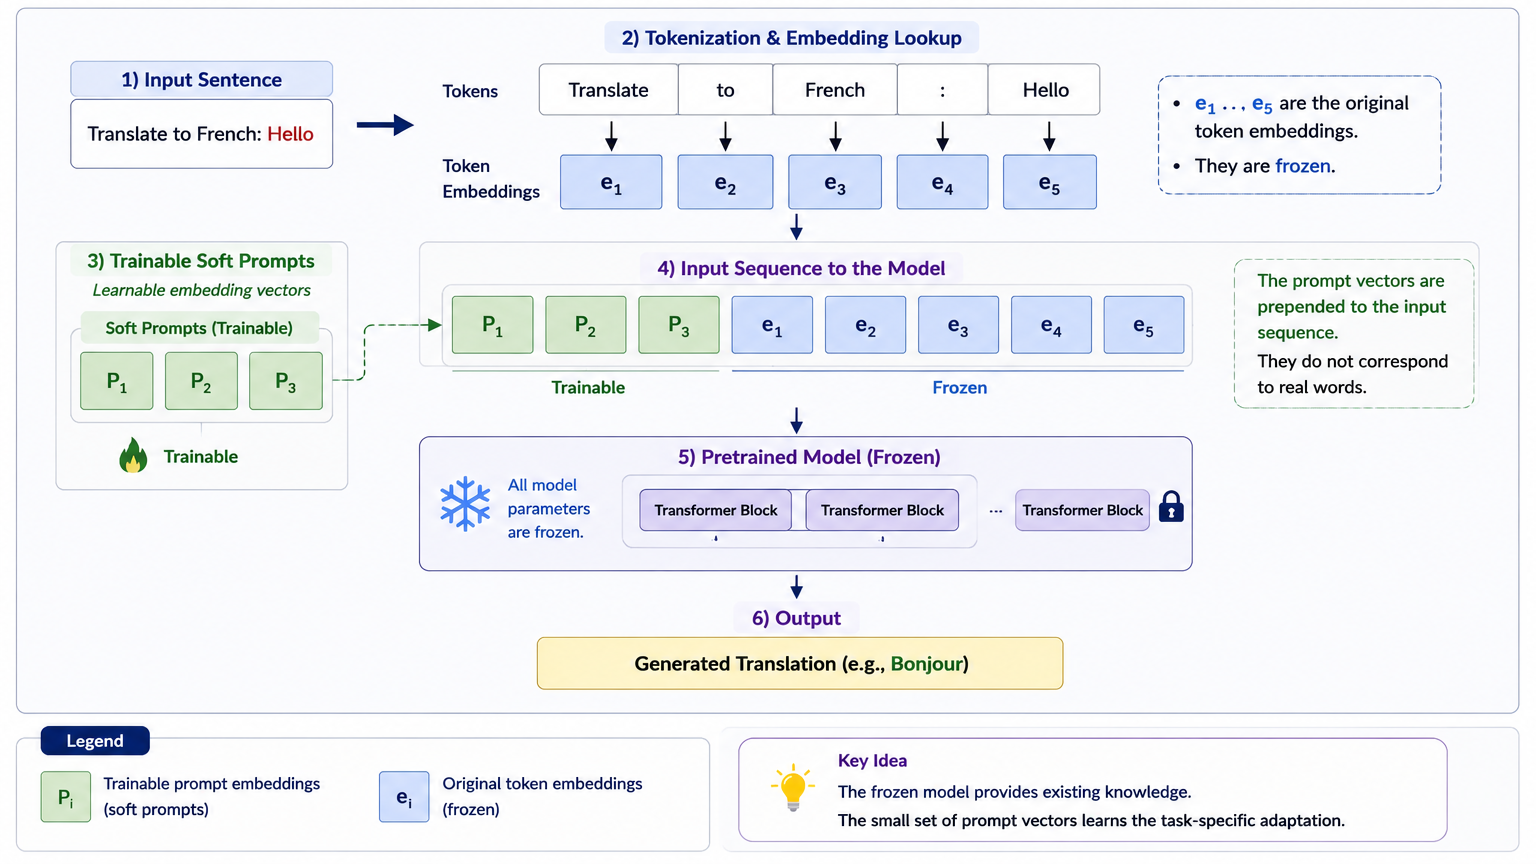
\includegraphics[width=0.95\textwidth]{figures/12-6 figure.png}
\end{figure}
Unlike ordinary tokens, the prompt vectors do not correspond to actual words. They are simply learnable vectors with the same dimensionality as the token embeddings.

During training,

\begin{itemize}
\item the Transformer parameters remain frozen;
\item only the prompt embeddings are updated using gradient descent.
\end{itemize}
\clearpage 
\begin{figure}[H]
\centering
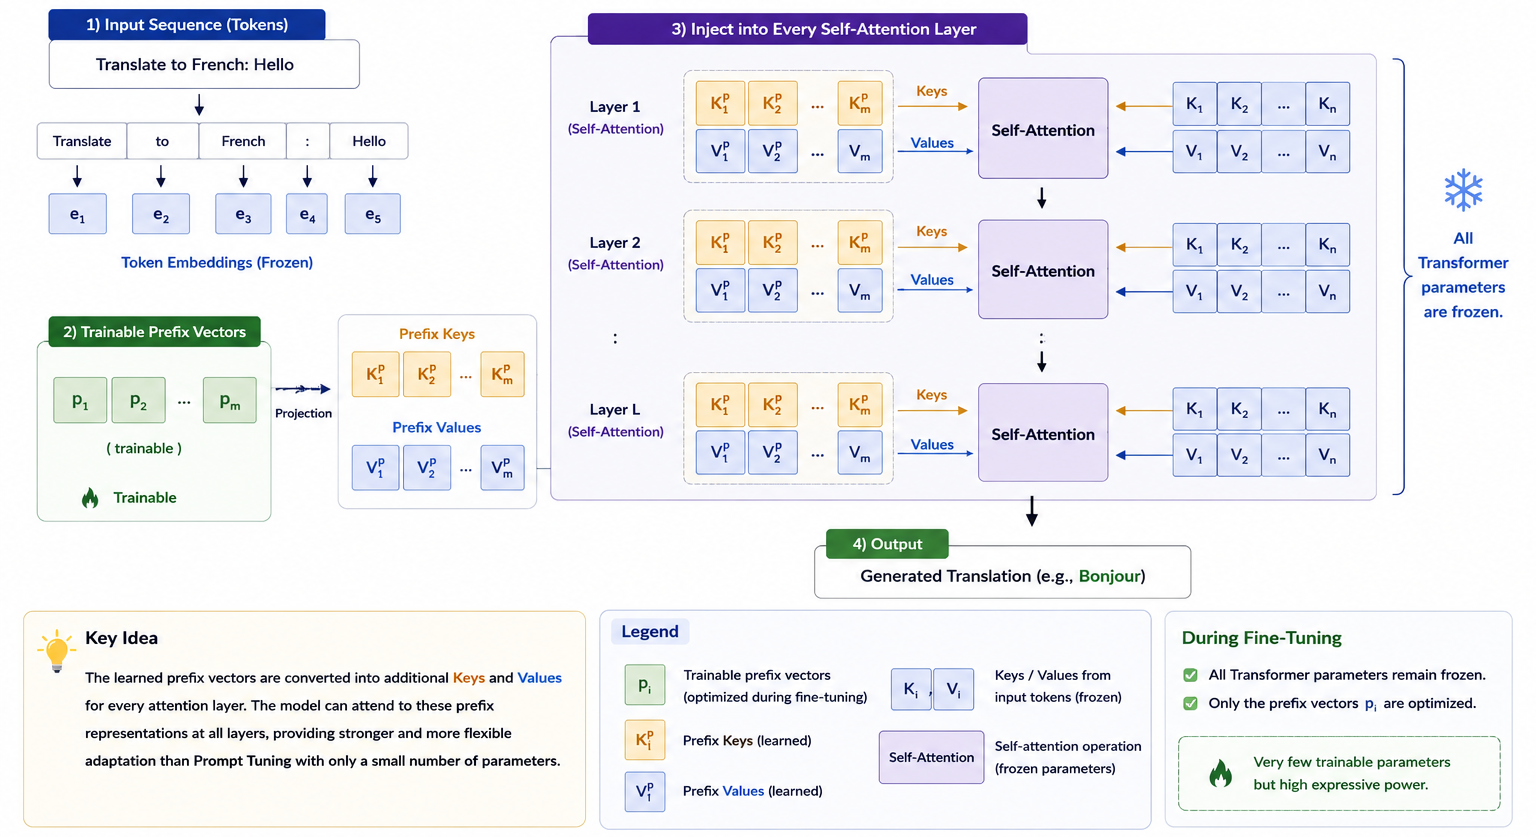
\includegraphics[width=0.95\textwidth]{figures/12-7 figure.png}
\end{figure}
Over time, these learned prompt vectors steer the pretrained model toward the desired downstream task without modifying its original parameters.
\subsection*{Prefix Tuning}

Prefix Tuning extends the idea of Prompt Tuning by injecting trainable vectors directly into the Transformer's attention mechanism rather than into the input sequence.

Instead of learning additional input embeddings, Prefix Tuning learns a set of trainable prefix vectors that are transformed into additional \textbf{Keys} and \textbf{Values} for every self-attention layer.

Consequently, each attention layer attends not only to the original input tokens but also to the learned prefix representations.

The computation can be summarized as

\[
\text{Trainable Prefix}
\longrightarrow
(K_{\text{prefix}},V_{\text{prefix}})
\longrightarrow
\text{Self-Attention}
\longrightarrow
\text{Output}.
\]

During fine-tuning,

\begin{itemize}
\item all Transformer parameters remain frozen;
\item only the prefix vectors are optimized.
\end{itemize}

Because the learned prefixes influence every attention layer, Prefix Tuning generally provides greater expressive power than Prompt Tuning while still requiring only a very small number of trainable parameters.


\section{LoRA (Low-Rank Adaptation)}

Large Language Models contain numerous weight matrices within their Transformer layers, such as the projection matrices used to compute queries, keys, values, and feed-forward transformations. During conventional full fine-tuning, every weight matrix is updated using task-specific data.

If a pretrained weight matrix is denoted by \(W\), the updated weights can be written as

\[
W' = W + \Delta W,
\]

where

\begin{itemize}
    \item \(W\) denotes the pretrained weight matrix;
    \item \(\Delta W\) is the trainable weight update learned during fine-tuning.
\end{itemize}

The main limitation of full fine-tuning is that the update matrix \(\Delta W\) has exactly the same dimensions as \(W\). Consequently, if \(W\) contains millions of parameters, then \(\Delta W\) also introduces millions of additional trainable parameters.

Researchers observed that although the weight matrices are very large, the learned updates often possess a much lower intrinsic rank. In other words, the model does not require millions of completely independent parameter updates. Instead, most of the useful task-specific information can be represented within a much smaller low-dimensional subspace.

This observation forms the key idea behind \textbf{Low-Rank Adaptation (LoRA)}.
\subsection*{Low-Rank Approximation}

Instead of learning the full update matrix \(\Delta W\), LoRA approximates it as the product of two much smaller matrices:

\[
\boxed{\Delta W = BA}
\]

where

\[
A \in \mathbb{R}^{r\times d},
\qquad
B \in \mathbb{R}^{k\times r},
\]

and

\[
r \ll d,\; k.
\]

The value \(r\) is called the \textbf{rank} of the LoRA decomposition and is typically chosen from

\[
r \in \{4,\,8,\,16,\,32,\,64\}.
\]

Since \(r\) is much smaller than both \(d\) and \(k\), the number of trainable parameters is drastically reduced.

The term \emph{Low-Rank Adaptation} originates directly from this low-rank decomposition of the weight update.
\begin{figure}[H]
\centering
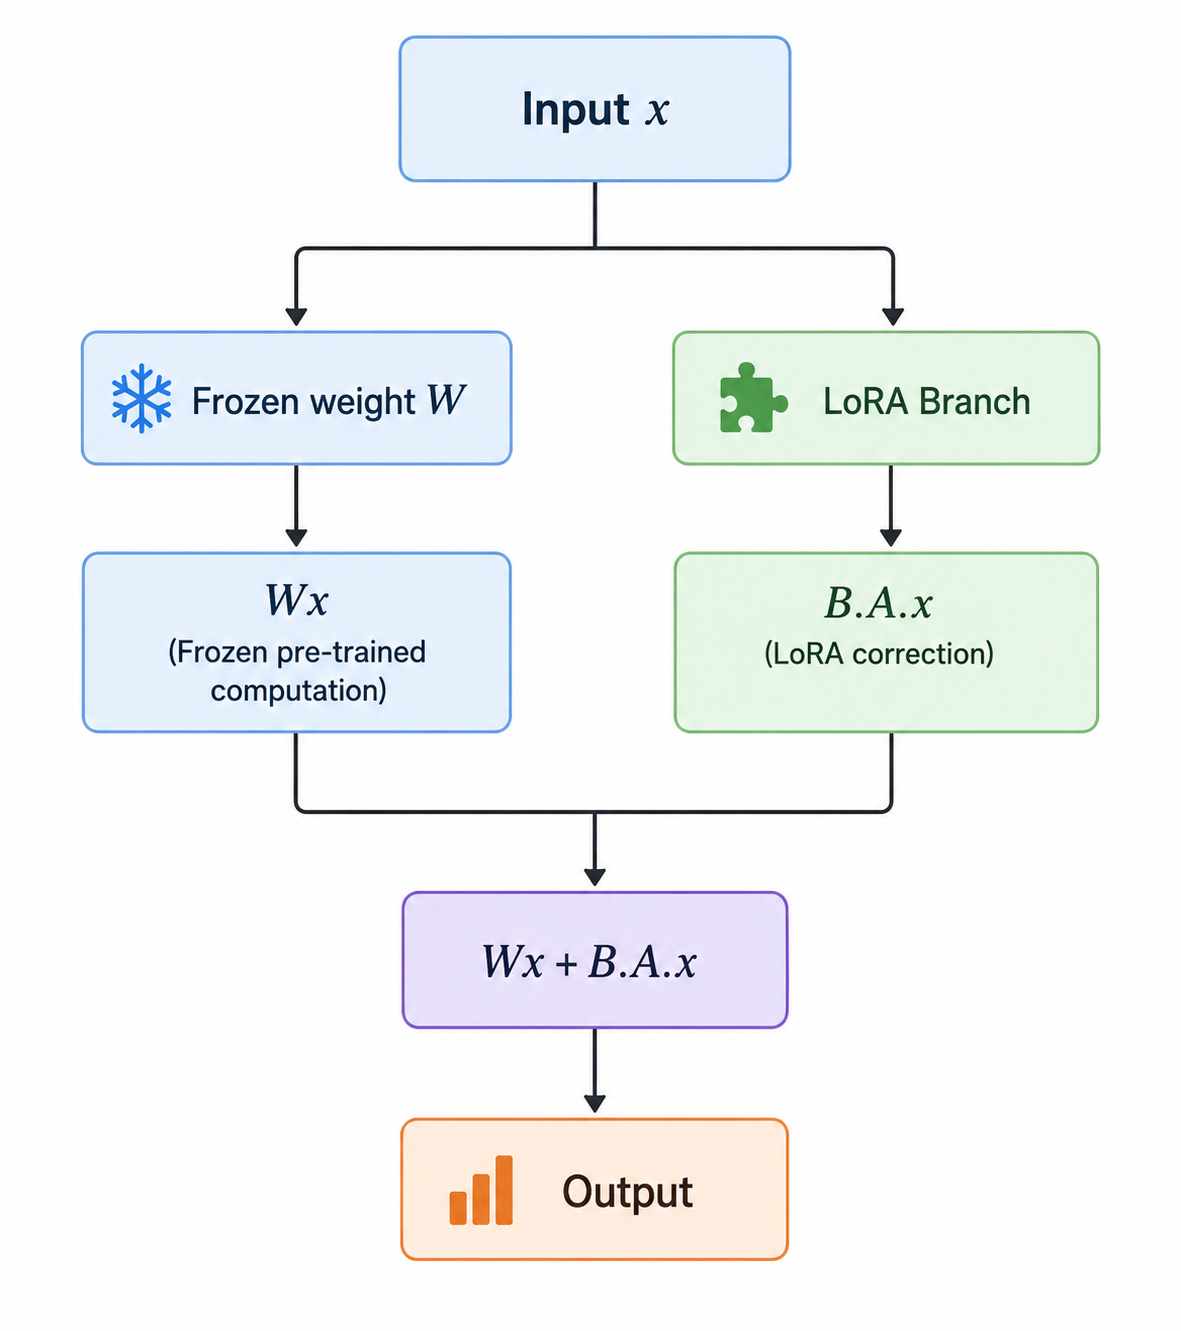
\includegraphics[width=0.9\textwidth]{figures/12-2 figure.png}
\label{fig:12-4}
\end{figure}
\subsection*{Numerical Example}

Suppose a pretrained weight matrix has dimensions

\[
W \in \mathbb{R}^{4096\times4096}.
\]

With full fine-tuning, the entire matrix must be updated, requiring

\[
4096 \times 4096
=
16.8\text{ million}
\]

trainable parameters.

Assume that LoRA uses a rank of

\[
r=8.
\]

Then only two small matrices are learned:

\[
A\in\mathbb{R}^{8\times4096},
\]

\[
B\in\mathbb{R}^{4096\times8}.
\]

Their product

\[
BA
=
(4096\times8)
(8\times4096)
=
4096\times4096
\]

has exactly the same dimensions as the original weight matrix and therefore can replace the full update \(\Delta W\).
\subsection*{Forward Pass}

During inference and training, the pretrained weight matrix remains frozen. The output is computed as

\[
y
=
Wx
+
BAx,
\]

where

\begin{itemize}
    \item \(Wx\) is the output produced by the frozen pretrained model;
    \item \(BAx\) is the low-rank correction learned by LoRA.
\end{itemize}

next Figure illustrates this computation, where the original branch remains frozen while the LoRA branch learns the task-specific adaptation.

\begin{figure}[H]
\centering
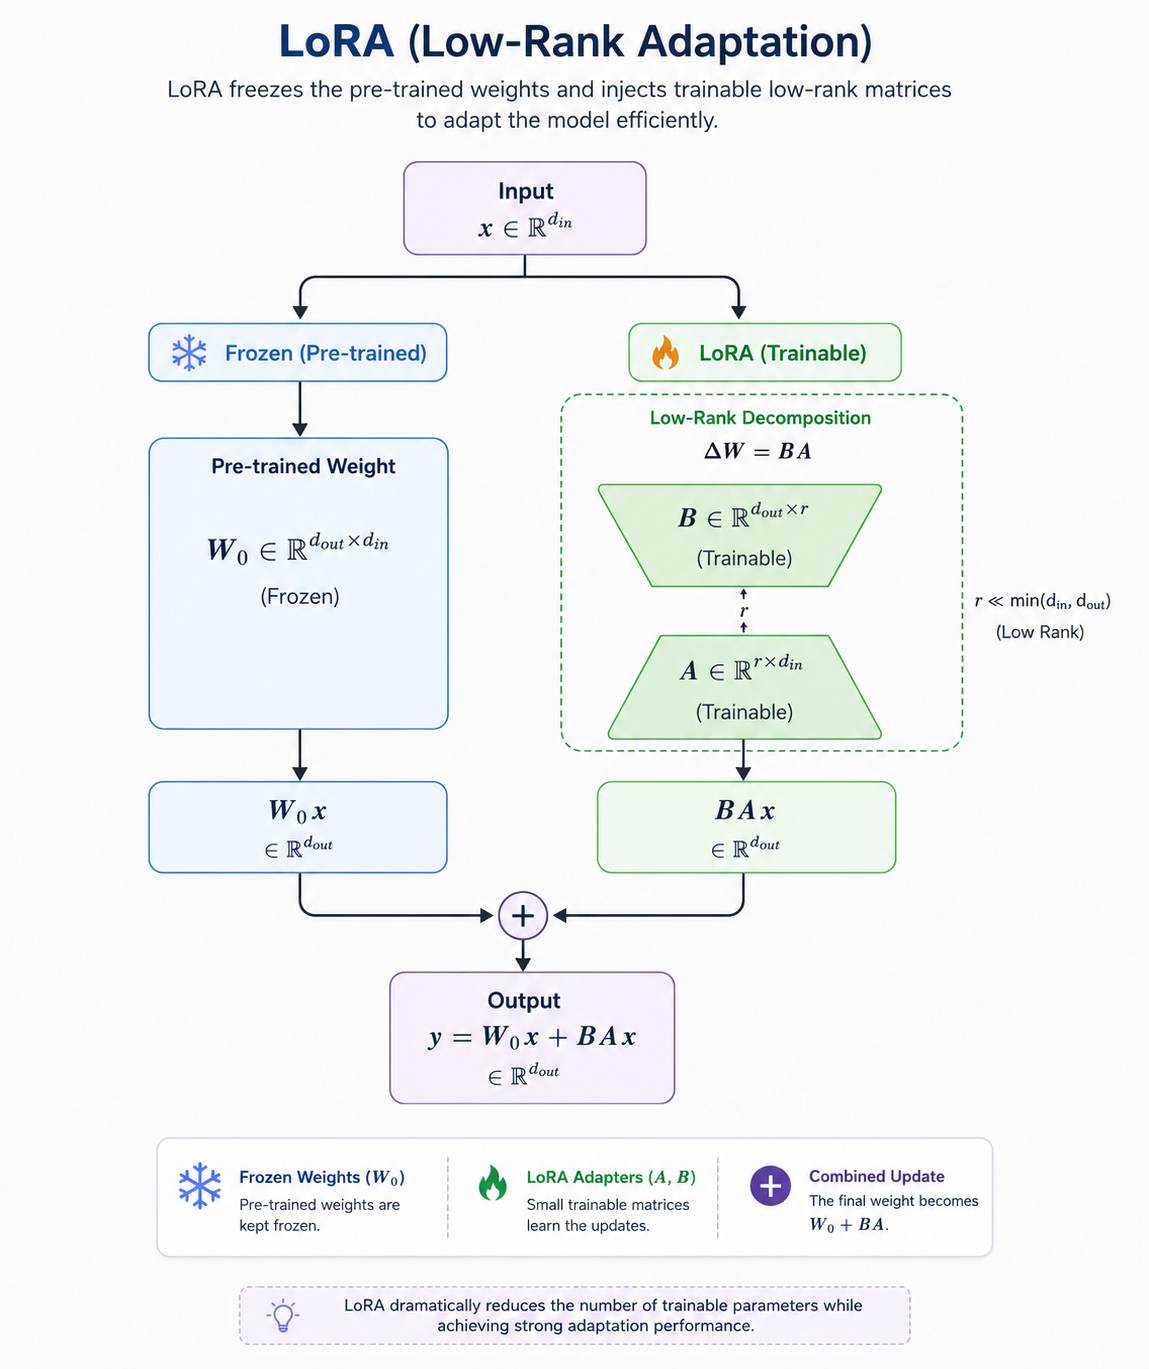
\includegraphics[width=0.85\textwidth]{figures/12-4 figure.png}
\label{fig:lora_architecture}
\end{figure}

\subsection*{Parameter Reduction}

Continuing the previous example,

\[
W
=
4096\times4096
=
16.8
\text{ million parameters}.
\]

LoRA learns only

\[
A:
8\times4096
=
32\,768,
\]

and

\[
B:
4096\times8
=
32\,768.
\]

Therefore, the total number of trainable parameters becomes

\[
32\,768
+
32\,768
=
65\,536
\approx
64\text{K}.
\]

Consequently, LoRA reduces the number of trainable parameters from approximately \(16.8\) million to only \(64\) thousand, corresponding to a reduction of more than \(250\times\).
\subsection*{Why Does LoRA Work?}

A pretrained Large Language Model already contains extensive knowledge acquired during large-scale pretraining, including language understanding, reasoning abilities, and factual information. For many downstream tasks, only a relatively small modification of the pretrained weights is required.

Instead of relearning the entire weight matrix, LoRA learns only this small task-specific correction through the low-rank update \(BA\). As a result, the pretrained knowledge is preserved while the model efficiently adapts to the new task using only a tiny fraction of the parameters required by full fine-tuning.
\subsection*{Transformer Weight Matrices}

A Transformer layer contains several trainable weight matrices distributed across its self-attention and feed-forward (MLP) components.

Within the self-attention mechanism, the input representation is projected into three different spaces using separate linear transformations:

\[
\text{Input}
\longrightarrow
W_Q,\;W_K,\;W_V
\longrightarrow
\text{Self-Attention}
\longrightarrow
W_O,
\]

where

\begin{itemize}
    \item $W_Q$ is the Query projection matrix;
    \item $W_K$ is the Key projection matrix;
    \item $W_V$ is the Value projection matrix;
    \item $W_O$ is the Output projection matrix.
\end{itemize}

In addition to the attention mechanism, every Transformer layer contains a feed-forward network (MLP), which is composed of two linear transformations separated by a nonlinear activation function:

\[
\text{Input}
\longrightarrow
\text{Linear}
\longrightarrow
\text{Activation}
\longrightarrow
\text{Linear}
\longrightarrow
\text{Output}.
\]

Each linear transformation in both the attention module and the MLP possesses its own trainable weight matrix.


\subsection*{Where Can We Apply LoRA?}

Since LoRA modifies only linear transformations, it can theoretically be attached to any weight matrix inside a Transformer layer.

Possible insertion points include

\[
W_Q,\;
W_K,\;
W_V,\;
W_O,
\]

as well as the two linear layers of the MLP.

When LoRA is applied to a weight matrix, the original transformation

\[
W
\]

is replaced by

\[
W + BA,
\]

where the pretrained matrix $W$ remains frozen and only the low-rank matrices $A$ and $B$ are optimized.

Suppose a Transformer contains one hundred linear layers. Applying LoRA to every layer would still require significantly fewer trainable parameters than full fine-tuning. Nevertheless, doing so would increase

\begin{itemize}
    \item the number of trainable parameters;
    \item GPU memory consumption;
    \item training time.
\end{itemize}

Consequently, an important design choice is determining which weight matrices should receive LoRA modules.
\subsection*{Which Layers Are Usually Chosen?}

Empirical studies have shown that not all weight matrices contribute equally to downstream adaptation.

For many modern Large Language Models, LoRA is commonly applied only to the Query and Value projection matrices:

\[
W_Q
\quad\text{and}\quad
W_V.
\]

These matrices directly influence the attention mechanism by determining how tokens attend to one another. Modifying only the Query and Value projections allows the model to learn new attention patterns while leaving the majority of the pretrained network unchanged.

Although LoRA can also be applied to the Key, Output, and MLP projection matrices, restricting the adaptation to $W_Q$ and $W_V$ often provides an excellent trade-off between computational efficiency and downstream performance. Consequently, this configuration has become the default choice in many practical implementations of LoRA.
\begin{table}[H]
\centering
\caption{Common insertion points for LoRA in a Transformer layer.}
\label{tab:lora_layers}

\renewcommand{\arraystretch}{1.3}

\begin{tabular}{ll}
\toprule
\textbf{Layer} & \textbf{Commonly Used} \\
\midrule
Query Projection ($W_Q$) & \checkmark \\
Key Projection ($W_K$) & Optional \\
Value Projection ($W_V$) & \checkmark \\
Output Projection ($W_O$) & Optional \\
MLP Linear Layer 1 & Optional \\
MLP Linear Layer 2 & Optional \\
\bottomrule
\end{tabular}

\end{table}

\subsection*{Why Is LoRA Usually Applied to Query and Value?}

Although LoRA can theoretically be applied to any linear layer in a Transformer, empirical studies have shown that some weight matrices contribute more than others to downstream adaptation.

The Query projection matrix ($W_Q$) determines how each token searches for relevant information, while the Value projection matrix ($W_V$) controls the information that is ultimately transmitted through the attention mechanism. Adapting these two matrices allows the model to learn new attention behaviors with relatively few trainable parameters.

In contrast, the Key projection matrix ($W_K$) defines how tokens are matched during attention. In many experiments, updating $W_K$ provides only modest performance improvements while increasing the computational cost. Consequently, many practical implementations omit LoRA on the Key projection.

For more challenging tasks, some implementations also apply LoRA to the Output projection ($W_O$) or even to the feed-forward (MLP) layers.

Typical LoRA configurations include

\[
W_Q + W_V,
\]

\[
W_Q + W_K + W_V,
\]

\[
W_Q + W_V + W_O,
\]

or

\[
\text{All Linear Layers}.
\]

The choice depends on several factors:

\begin{itemize}
    \item available GPU memory;
    \item task complexity;
    \item desired accuracy.
\end{itemize}
\subsection*{Typical Configurations in Modern LLMs}

Many popular Large Language Models apply LoRA primarily to the Query and Value projection matrices. Examples include

\begin{center}
\renewcommand{\arraystretch}{1.2}
\begin{tabular}{ll}
\toprule
\textbf{Model Family} & \textbf{Typical LoRA Targets} \\
\midrule
Llama & $W_Q,\;W_V$ \\
Mistral & $W_Q,\;W_V$ \\
Gemma & $W_Q,\;W_V$ \\
Phi & $W_Q,\;W_V$ \\
Qwen & $W_Q,\;W_V$ (sometimes all linear layers) \\
\bottomrule
\end{tabular}
\end{center}

More recent implementations often apply LoRA to all linear layers of the Transformer. Although this slightly increases the number of trainable parameters, it generally provides better downstream performance while remaining far more efficient than full fine-tuning.
\subsection*{LoRA Scaling Factor}

Besides the rank $r$, another important hyperparameter is the scaling factor, denoted by $\alpha$.

Rather than computing the update simply as

\[
W + BA,
\]

LoRA actually applies

\[
W+\frac{\alpha}{r}BA.
\]

The factor

\[
\frac{\alpha}{r}
\]

controls the contribution of the LoRA update relative to the frozen pretrained weights.

Intuitively, a larger value of $\alpha$ increases the influence of the learned adaptation, whereas a smaller value keeps the model closer to the original pretrained parameters.

Typical values are

\[
\alpha \in [16,\,64].
\]
\subsection*{LoRA Dropout}

Many LoRA implementations optionally apply dropout to the LoRA branch during training.

The objective is to

\begin{itemize}
    \item reduce overfitting;
    \item improve generalization;
    \item increase robustness, particularly when fine-tuning on small datasets.
\end{itemize}

Typical dropout values range from

\[
0.0
\quad\text{to}\quad
0.1.
\]
\section{Training with LoRA}

During LoRA fine-tuning, the pretrained Transformer remains completely frozen, and only the low-rank matrices \(A\) and \(B\) are optimized.

During the forward pass, each adapted linear layer computes

\[
y
=
Wx
+
\frac{\alpha}{r}BAx,
\]

where \(Wx\) is produced by the frozen pretrained model and the second term represents the task-specific LoRA correction.

During backpropagation, gradients are computed only for the matrices \(A\) and \(B\). Since the original model parameters remain fixed, both GPU memory usage and computational cost are significantly lower than in full fine-tuning.

After training, it is unnecessary to store the entire pretrained model again. Only the LoRA adapter weights together with their configuration (e.g., rank, scaling factor, and target modules) are saved. These adapter files are typically several orders of magnitude smaller than the full model checkpoint.

During inference, two deployment strategies are commonly used:

\begin{enumerate}
    \item \textbf{Separate adapters}: the pretrained model and the LoRA adapters are loaded independently, allowing multiple task-specific adapters to share the same base model.
    \item \textbf{Merged adapters}: the LoRA update is merged permanently into the pretrained weights, producing a single model with no additional inference overhead.
\end{enumerate}
\section{Advantages and Limitations of LoRA}

LoRA has become one of the most widely adopted Parameter-Efficient Fine-Tuning (PEFT) techniques because it achieves a strong balance between efficiency and performance. By learning only a small low-rank update while keeping the pretrained model frozen, LoRA significantly reduces the computational resources required for fine-tuning large language models.

Nevertheless, LoRA is not without limitations. Since it approximates the weight updates using a low-rank decomposition, its expressive capacity is constrained by the chosen rank. In some complex tasks, a low-rank approximation may not capture all the information that would be learned through full fine-tuning.

Table~\ref{tab:lora_advantages_limitations} summarizes the main advantages and limitations of LoRA.
\begin{table}[H]
\centering
\caption{Advantages and limitations of LoRA.}
\label{tab:lora_advantages_limitations}

\renewcommand{\arraystretch}{1.35}

\begin{tabular}{p{7cm}p{7cm}}
\toprule
\textbf{Advantages} & \textbf{Limitations} \\
\midrule

Requires only a small number of trainable parameters &
Performance depends on the selected rank ($r$). \\

Significantly reduces GPU memory usage &
Very small ranks may underfit complex tasks. \\

Faster training than full fine-tuning &
Choosing appropriate target layers requires experimentation. \\

Produces compact adapter checkpoints &
May perform slightly below full fine-tuning on highly specialized tasks. \\

Multiple adapters can share the same pretrained model &
Additional hyperparameters ($r$, $\alpha$, dropout) must be tuned. \\

Adapters can be merged into the pretrained model for efficient inference &
Not every task benefits equally from low-rank adaptation. \\

Preserves the pretrained knowledge while learning task-specific adaptations &
Still requires loading the full pretrained model during training and inference. \\

\bottomrule
\end{tabular}

\end{table}
\subsection*{Summary}

Parameter-Efficient Fine-Tuning (PEFT) addresses the limitations of full fine-tuning by updating only a small subset of parameters while keeping the pretrained model frozen. Among the various PEFT techniques, LoRA has emerged as one of the most effective and widely adopted methods.

Instead of learning a full weight update, LoRA approximates the update using a low-rank decomposition, dramatically reducing the number of trainable parameters, GPU memory requirements, and storage costs while maintaining performance close to full fine-tuning on many downstream tasks.

Thanks to its simplicity, computational efficiency, and compatibility with existing Transformer architectures, LoRA has become the standard fine-tuning approach for modern Large Language Models and serves as the foundation for several recent PEFT variants, including QLoRA, AdaLoRA, DoRA, and other low-rank adaptation methods.

\section{Quantization}

LoRA dramatically reduces the number of trainable parameters during fine-tuning. However, it does not reduce the size of the pretrained model itself. Although the base model remains frozen, it must still be loaded into GPU memory during both training and inference.

For example, consider an LLM containing 8 billion parameters. Even if only the LoRA adapters are trainable, the entire pretrained model must still reside in memory, making memory consumption a significant bottleneck.

This observation motivates another important technique known as \textbf{quantization}.
\subsection*{Why Are Large Models Memory-Intensive?}

Every parameter of a neural network is simply a numerical value, for example,

\[
0.2345,\qquad
-1.5823,\qquad
0.0049.
\]

These values are stored using numerical data types. The most common format during training is \textbf{FP32 (32-bit floating-point)}, where each parameter occupies

\[
32\ \text{bits}
=
4\ \text{bytes}.
\]

Consequently, the memory required to store a model grows linearly with the number of parameters.

For example,

\[
1\text{ Billion Parameters}
\times
4\text{ Bytes}
=
4\text{ GB}.
\]

Therefore, an LLM with

\[
8\text{ Billion Parameters}
\]

requires approximately

\[
8\times4
=
32\text{ GB}
\]

simply to store its weights.

During training, additional GPU memory is required for

\begin{itemize}
    \item gradients;
    \item optimizer states;
    \item intermediate activations.
\end{itemize}

As a result, the total memory requirement is substantially larger than the model size alone.
\subsection*{Main Idea}

The key question behind quantization is remarkably simple:

\begin{center}
\emph{Do we really need 32 bits to represent every weight?}
\end{center}

If a parameter can be stored using fewer bits without significantly affecting model performance, then both memory usage and computational cost can be greatly reduced.

Instead of storing each parameter using 32 bits, quantization represents weights using lower-precision numerical formats such as

\[
16,\;
8,\;
\text{or}
\;
4
\text{ bits}.
\]

Fewer bits require less memory, allowing larger models to run on more affordable hardware.
\section{Common Numerical Formats}

\begin{table}[H]
\centering
\caption{Common numerical formats used for neural network parameters.}
\label{tab:numerical_formats}

\renewcommand{\arraystretch}{1.25}

\begin{tabular}{ccc}
\toprule
\textbf{Format} &
\textbf{Bits per Parameter} &
\textbf{Typical Usage} \\
\midrule
FP32 & 32 & Standard training \\
FP16 & 16 & Mixed-precision training \\
BF16 & 16 & Large-scale LLM training \\
INT8 & 8 & Quantized inference \\
INT4 & 4 & Highly compressed LLMs \\
\bottomrule
\end{tabular}

\end{table}
\subsection*{The Precision--Memory Trade-Off}

As the numerical precision decreases,

\begin{itemize}
    \item GPU memory consumption decreases;
    \item computational efficiency improves;
    \item numerical precision also decreases.
\end{itemize}

This trade-off lies at the heart of quantization. The objective is to reduce memory usage while maintaining nearly the same predictive performance.
\subsection*{Memory Reduction Example}

Consider an LLM with 8 billion parameters.

If the weights are stored using FP32,

\[
8\text{B}
\times
4\text{ Bytes}
=
32\text{ GB}.
\]

If the same model is quantized to INT4,

\[
8\text{B}
\times
0.5\text{ Byte}
=
4\text{ GB}.
\]

Thus, quantization reduces the storage requirement from approximately

\[
32\text{ GB}
\rightarrow
4\text{ GB},
\]

corresponding to an

\[
8\times
\]

reduction in memory usage.
\subsection*{Why Does Quantization Work?}

At first glance, reducing numerical precision may appear risky. For example,

\[
0.638274918
\]

might be approximated as

\[
0.64.
\]

Although this approximation introduces a small numerical error, modern neural networks are remarkably tolerant to such inaccuracies.

Rather than relying on the exact value of a single parameter, predictions emerge from the collective interaction of billions of weights. Consequently, small approximation errors in individual parameters rarely have a noticeable impact on the overall model performance.

This observation explains why modern Large Language Models can often be quantized to 8-bit or even 4-bit precision while maintaining accuracy close to that of the original full-precision model.
\subsection*{Quantization Is Not Compression}

The terms \emph{quantization} and \emph{compression} are often used interchangeably, although they describe different concepts.

Compression generally refers to reducing the storage size of a model using encoding techniques, such as entropy coding or file compression algorithms. Quantization, on the other hand, changes the numerical representation of the model parameters by storing them with fewer bits.

For example, a weight originally stored as a 32-bit floating-point value (FP32) may instead be represented using 8-bit or 4-bit precision. The objective is not to compress the file itself, but to reduce the memory required to represent each parameter.
\subsection*{Where Is Quantization Used?}

Quantization is primarily used in two scenarios.

\textbf{1. Inference}

The most common application is model deployment. A pretrained model is first quantized and then used for inference.

\[
\text{Train Model}
\longrightarrow
\text{Quantize}
\longrightarrow
\text{Faster Inference}
\longrightarrow
\text{Lower Memory Usage}
\]

Many local LLM deployment frameworks, such as \texttt{llama.cpp} and \texttt{Ollama}, rely on quantized models to run large language models efficiently on consumer hardware.

\vspace{0.4cm}

\textbf{2. Training}

Applying quantization during training is considerably more challenging.

Although the model weights may be stored using low precision, optimization still requires stable gradient computations. Consequently, training usually maintains gradients and certain intermediate computations in higher precision.

This challenge motivated the development of \textbf{QLoRA}, in which

\begin{itemize}
    \item the pretrained backbone is stored in 4-bit precision;
    \item the LoRA adapters remain trainable in higher precision.
\end{itemize}
\subsection*{LoRA and Quantization}

Although LoRA and quantization are often used together, they address two different challenges.

LoRA answers the question

\begin{center}
\emph{Which parameters should be trained?}
\end{center}

by freezing the pretrained model and learning only a small number of additional parameters.

In contrast, quantization answers the question

\begin{center}
\emph{How should model parameters be stored?}
\end{center}

by representing the weights with lower numerical precision.

Therefore, these two techniques are complementary rather than competing approaches:

\[
\begin{array}{ccc}
\textbf{LoRA} & \Longrightarrow & \text{Train Fewer Parameters} \\[0.3cm]
\textbf{Quantization} & \Longrightarrow & \text{Store Parameters Using Fewer Bits}
\end{array}
\]

By combining both ideas, modern fine-tuning methods achieve

\[
\boxed{
\textbf{QLoRA}
=
\textbf{LoRA}
+
\textbf{Quantization}
}
\]

Thus, QLoRA simultaneously reduces the number of trainable parameters and the memory required to store the pretrained model, making it possible to fine-tune very large language models on modest hardware.

\section{Modern Quantization Methods}

Several quantization techniques have been proposed in recent years. Although all of them aim to reduce the memory footprint of large language models, they differ in their objectives. Some methods prioritize model accuracy, others focus on inference speed, while some are designed for efficient deployment on consumer hardware.

Consequently, modern LLM ecosystems include different quantization algorithms, model formats, and software libraries, each serving a specific purpose.
\begin{table}[H]
\centering
\caption{Representative quantization algorithms for Large Language Models.}
\label{tab:quantization_methods}

\renewcommand{\arraystretch}{1.3}

\begin{tabular}{p{2.3cm}p{8.2cm}p{3cm}}
\toprule
\textbf{Method} &
\textbf{Main Idea} &
\textbf{Typical Use} \\
\midrule

GPTQ (2023)
&
Post-training weight quantization that minimizes quantization error to preserve model accuracy.
&
High-quality inference
\\

AWQ (2023)
&
Activation-aware quantization that protects the most important weights using activation statistics.
&
Instruction-tuned LLM inference
\\

HQQ (2024)
&
Half-Quadratic Quantization supporting flexible bit-widths with little or no calibration.
&
Research and flexible quantization
\\

\bottomrule
\end{tabular}

\end{table}
\subsection*{Quantized Model Formats}

Besides quantization algorithms, several model formats have been developed to simplify deployment.

The most popular format is \textbf{GGUF (GPT-Generated Unified Format)}, introduced in 2023 for the \texttt{llama.cpp} ecosystem.

Unlike GPTQ or AWQ, GGUF is not a quantization algorithm. Instead, it is a file format that stores

\begin{itemize}
\item model weights,
\item tokenizer,
\item metadata,
\item quantization information
\end{itemize}

inside a single portable file.

GGUF is widely used for local inference through \texttt{llama.cpp} and Ollama.
\subsection*{GPU-Optimized Formats}

Another popular format is \textbf{EXL2}, which is optimized for the ExLlamaV2 inference engine.

Its primary objective is maximizing inference speed on NVIDIA GPUs while maintaining high model quality under low-bit quantization.

EXL2 is therefore commonly used when fast GPU inference is the primary requirement.
\section{bitsandbytes}

Among all quantization tools, \textbf{bitsandbytes} has become the most widely adopted in the PEFT ecosystem.

Unlike GPTQ, AWQ, or HQQ, bitsandbytes is \textbf{not a quantization algorithm}. Instead, it is an open-source software library that provides efficient implementations of low-precision arithmetic for large language models.
It supports

\begin{itemize}
\item 8-bit loading,
\item 4-bit loading,
\item optimized CUDA kernels,
\item efficient integration with Hugging Face Transformers.
\end{itemize}
A pretrained FP16 model can be loaded directly in lower precision:

\[
\text{FP16 Model}
\longrightarrow
\texttt{bitsandbytes}
\longrightarrow
\text{INT8 Model}
\]

or

\[
\text{FP16 Model}
\longrightarrow
\texttt{bitsandbytes}
\longrightarrow
\text{INT4 Model}.
\]

This substantially reduces GPU memory consumption while preserving most of the original model performance.
\subsection*{NF4 Quantization}

One of the most important contributions of bitsandbytes is the introduction of \textbf{NF4 (NormalFloat4)}, a 4-bit numerical format specifically designed for neural network weights.

Unlike conventional INT4 quantization, NF4 assumes that pretrained neural network weights approximately follow a Gaussian distribution.

This assumption allows NF4 to allocate its limited numerical values more efficiently, producing lower quantization error and better downstream performance.

NF4 is one of the key components that enables QLoRA to achieve performance comparable to full-precision fine-tuning while storing the backbone model using only 4-bit precision.
\subsection*{Optimized CUDA Kernels}

bitsandbytes also provides highly optimized CUDA kernels for NVIDIA GPUs.

These implementations accelerate low-precision matrix operations, making both inference and QLoRA training significantly faster than naïve implementations.


During QLoRA training, the pretrained backbone is loaded in 4-bit precision using bitsandbytes, whereas only the LoRA matrices are updated.

Consequently, GPU memory consumption is dramatically reduced while preserving the accuracy of the pretrained model.
\begin{table}[H]
\centering
\caption{Reasons why bitsandbytes became the standard library for QLoRA.}

\renewcommand{\arraystretch}{1.3}

\begin{tabular}{p{7cm}p{7cm}}
\toprule
\textbf{Feature} & \textbf{Benefit} \\
\midrule

4-bit and 8-bit loading &
Greatly reduces GPU memory usage \\

NF4 quantization &
Higher accuracy than standard INT4 \\

Optimized CUDA kernels &
Fast inference and training \\

Hugging Face integration &
Simple deployment with Transformers \\

Native QLoRA support &
Standard library for PEFT workflows \\

\bottomrule
\end{tabular}

\end{table}


\section{QLoRA (Quantized Low-Rank Adaptation)}

Although LoRA dramatically reduces the number of trainable parameters, one important limitation remains. During training, the entire pretrained model must still be loaded into GPU memory. Even though its weights remain frozen, they are typically stored in FP16 or BF16 precision, which still requires a substantial amount of memory for modern Large Language Models.

Researchers therefore asked an important question:

\begin{center}
\textit{If the pretrained model is frozen, why store it in high precision?}
\end{center}

The answer led to \textbf{QLoRA (Quantized Low-Rank Adaptation)}, proposed by Dettmers et al. (2023). The key idea is simple:

\begin{itemize}
    \item Quantize the frozen pretrained model to 4-bit precision.
    \item Keep the LoRA adapter matrices trainable in higher precision.
\end{itemize}

As a result, only a very small number of parameters are updated, while the backbone model occupies much less GPU memory.

\begin{figure}[H]
\centering
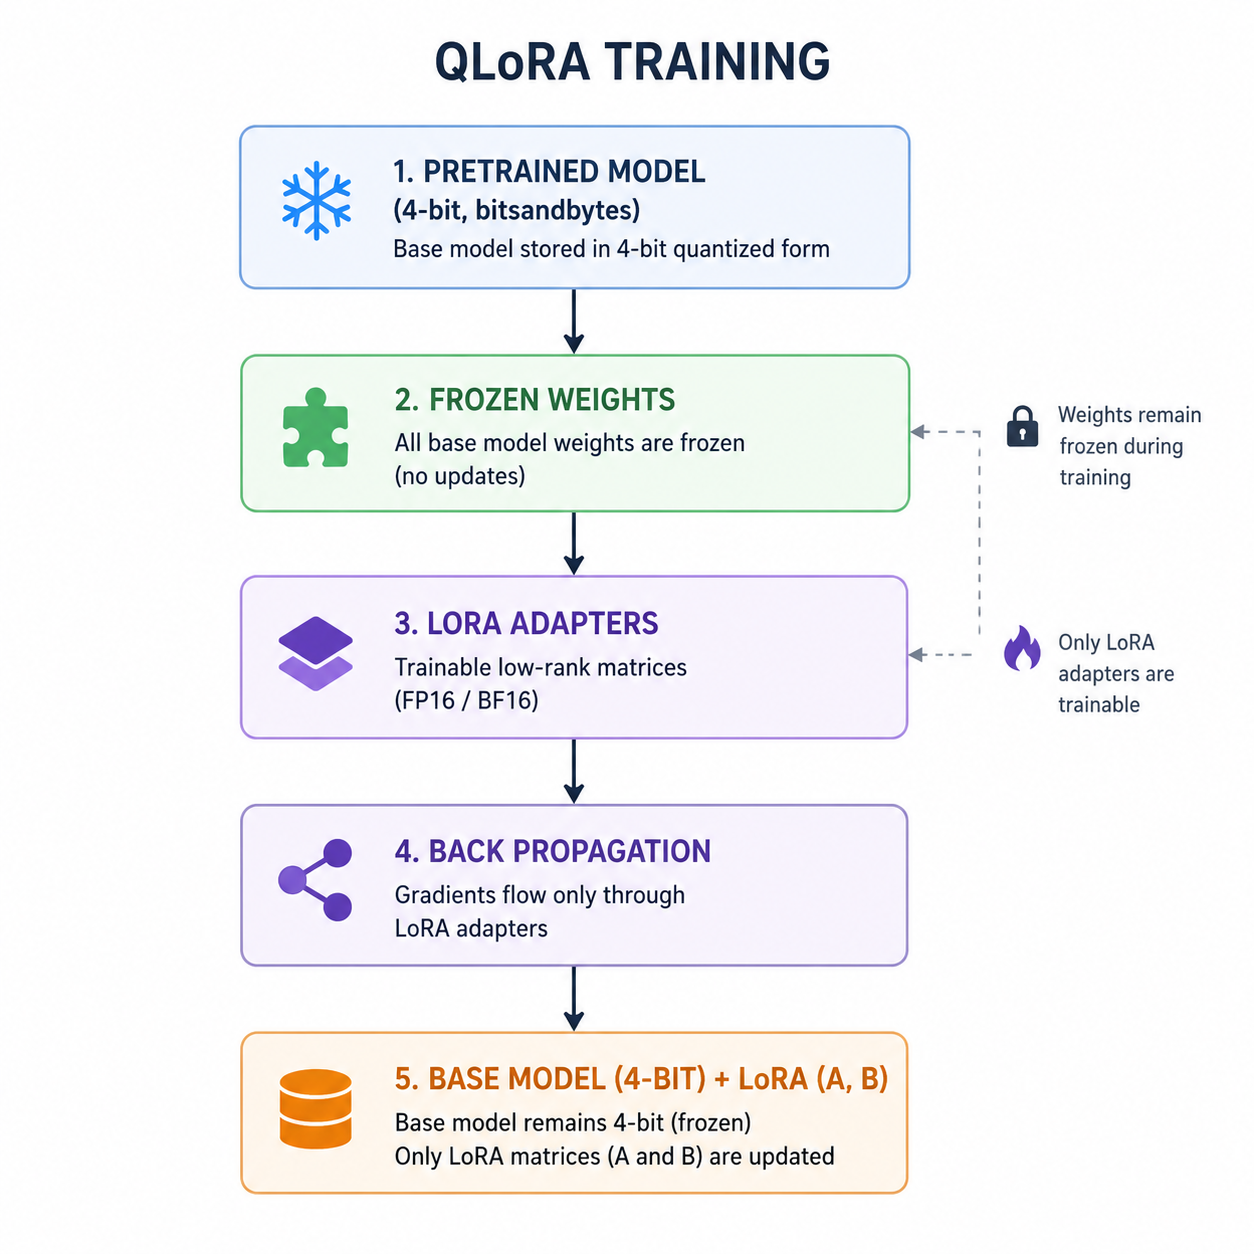
\includegraphics[width=0.85\textwidth]{figures/12-5 figure.png}
\end{figure}

Compared with standard LoRA, the only architectural difference is that the pretrained backbone is quantized before training.

\[
\boxed{
\text{4-bit Quantized Base Model (Frozen)}
+
\text{Trainable LoRA Adapters}
\longrightarrow
\text{Fine-Tuned Model}
}
\]

A common misconception is that QLoRA trains the quantized 4-bit weights. This is incorrect. The quantized backbone is used only during the forward computation and remains completely frozen throughout training. Backpropagation updates only the LoRA matrices ($A$ and $B$), exactly as in standard LoRA.

\subsection*{Key Innovations of QLoRA}

QLoRA combines LoRA with several techniques that make 4-bit fine-tuning practical.

\begin{enumerate}
    \item \textbf{NF4 (NormalFloat4)}\\
    Instead of using standard INT4 quantization, QLoRA adopts the NF4 numerical format, which is specifically designed for neural network weights. Since pretrained weights approximately follow a Gaussian distribution, NF4 represents them more accurately and reduces quantization error.

    \item \textbf{Double Quantization}\\
    Besides quantizing the model weights, QLoRA also quantizes the scaling factors used during quantization. This further reduces memory consumption with almost no loss in performance.

    \item \textbf{Paged Optimizers}\\
    GPU memory usage often fluctuates during training because optimizer states temporarily require additional memory. Paged optimizers dynamically move these temporary states between GPU and CPU memory, preventing memory spikes and enabling stable fine-tuning of much larger models.
\end{enumerate}

\subsection*{Advantages}

Compared with standard LoRA, QLoRA offers several important advantages:

\begin{itemize}
    \item Significantly lower GPU memory consumption.
    \item Fine-tuning of much larger language models on a single GPU.
    \item Performance comparable to full fine-tuning on many downstream tasks.
    \item Retains all advantages of LoRA while adding memory-efficient model storage.
\end{itemize}

Consequently, QLoRA has become one of the most influential techniques for parameter-efficient fine-tuning. By combining low-rank adaptation with 4-bit quantization, it enables high-quality fine-tuning of modern Large Language Models using affordable hardware.
\begin{table}[H]
\centering
\caption{Comparison of Full Fine-Tuning, LoRA, and QLoRA.}
\label{tab:ft_lora_qlora}

\renewcommand{\arraystretch}{1.35}

\begin{tabular}{|p{3.5cm}|p{2.8cm}|p{3.0cm}|p{2.6cm}|}
\hline
\rowcolor{gray!15}
\textbf{Method} &
\textbf{Base Model} &
\textbf{Trainable Parameters} &
\textbf{GPU Memory} \\
\hline

Full Fine-Tuning &
FP16 / BF16 &
All model parameters &
Very High \\
\hline

LoRA &
FP16 / BF16 &
Only LoRA matrices ($A$, $B$) &
Moderate \\
\hline

QLoRA &
4-bit (NF4) &
Only LoRA matrices ($A$, $B$) &
Low \\
\hline

\end{tabular}

\end{table}
\section*{Chapter Summary}

Modern Large Language Models contain billions of parameters, making full fine-tuning computationally expensive in terms of GPU memory, training time, and storage requirements. Parameter-Efficient Fine-Tuning (PEFT) addresses this challenge by freezing the pretrained backbone and training only a small number of additional parameters.

Among PEFT methods, LoRA has become the most widely adopted approach because it represents weight updates using low-rank matrices, dramatically reducing the number of trainable parameters while maintaining competitive performance.

QLoRA further extends this idea by storing the frozen backbone in 4-bit precision using NF4 quantization while continuing to train only the LoRA adapters. Combined with techniques such as Double Quantization and Paged Optimizers, QLoRA enables high-quality fine-tuning of very large language models on a single consumer GPU.

Today, LoRA and QLoRA have become the standard approaches for adapting modern Large Language Models because they provide an excellent balance between computational efficiency, memory usage, and downstream task performance.


\section{Beyond LoRA: Recent PEFT Methods}

Although LoRA and QLoRA have become the dominant approaches for parameter-efficient fine-tuning, numerous variants have been proposed to overcome some of their limitations. These methods generally aim to improve parameter allocation, optimization stability, memory efficiency, or adaptation capacity while preserving the fundamental PEFT philosophy of updating only a small subset of parameters.

Table~\ref{tab:modern_peft} summarizes some representative LoRA variants.
\begin{table}[H]
\centering
\caption{Representative extensions of LoRA.}
\label{tab:modern_peft}

\renewcommand{\arraystretch}{1.35}

\begin{tabular}{|p{2.6cm}|p{9cm}|}
\hline
\rowcolor{gray!15}
\textbf{Method} &
\textbf{Main Idea} \\
\hline

AdaLoRA &
Dynamically adjusts the rank of each layer during training, allocating more parameters to important layers and fewer to less important ones. \\
\hline

DoRA &
Separates each weight into magnitude and direction, allowing them to be optimized independently for improved stability and accuracy. \\
\hline

IA$^3$ &
Learns small scaling vectors that amplify or suppress activations instead of learning low-rank matrices, resulting in extremely low memory consumption. \\
\hline

LoRA+ &
Uses different learning rates for the LoRA matrices $A$ and $B$, leading to faster convergence and improved optimization. \\
\hline

VeRA &
Replaces most trainable matrices with fixed random matrices and learns only a small number of vectors, further reducing trainable parameters. \\
\hline

MoRA &
Improves the expressive power of low-rank adaptation by using richer matrix structures while remaining parameter efficient. \\
\hline

\end{tabular}

\end{table}
Despite these improvements, LoRA and QLoRA remain the most widely adopted PEFT techniques because they provide an excellent balance between simplicity, efficiency, and downstream performance. Most recent methods should therefore be viewed as refinements of LoRA rather than completely new fine-tuning paradigms.
\section{Practical PEFT Fine-Tuning Pipeline}

The practical workflow for fine-tuning a Large Language Model using LoRA or QLoRA typically consists of the following steps.
\subsection*{Step 1: Prepare the Dataset}

The first requirement is a task-specific dataset. Depending on the application, the dataset may contain:

\begin{itemize}
\item Question--Answer pairs
\item Instruction--Response pairs
\item Multi-turn conversations
\item Code and explanations
\item Translation examples
\item Summarization pairs
\end{itemize}

For example,

\begin{quote}
Instruction: Explain Newton's First Law.

Response: Newton's First Law states that...
\end{quote}

The objective is for the model to learn to generate the desired response.
\subsection*{Step 2: Format the Dataset}

Most LLM training frameworks expect structured datasets, typically stored in JSON or JSONL format.

\begin{verbatim}
{
  "instruction": "Translate to French",
  "input": "Hello",
  "output": "Bonjour"
}
\end{verbatim}

Different models may require slightly different dataset formats.
\subsection*{Step 3: Apply the Chat Template}

Modern instruction-tuned LLMs are trained using predefined conversation templates rather than raw text.

For example,

User:
What is Artificial Intelligence?

Assistant:
Artificial Intelligence is...

Each model family (Llama, Qwen, Gemma, Mistral, etc.) defines its own chat template, which must be used during training.
\subsection*{Step 4: Tokenization}

The formatted text is converted into token IDs using the tokenizer associated with the pretrained model.
\subsection*{Step 5: Configure LoRA or QLoRA}

Typical LoRA hyperparameters include

\begin{itemize}
\item Rank ($r$)
\item Scaling factor ($\alpha$)
\item Dropout
\item Target modules
\item Learning rate
\item Batch size
\item Number of epochs
\end{itemize}

When using QLoRA, additional settings include

\begin{itemize}
\item 4-bit loading
\item NF4 quantization
\item Compute data type (FP16 or BF16)
\end{itemize}
\subsection*{Step 6: Fine-Tuning}

Training follows the standard optimization pipeline

\[
\text{Input}
\rightarrow
\text{Forward Pass}
\rightarrow
\text{Loss}
\rightarrow
\text{Backpropagation}
\rightarrow
\text{Update LoRA Parameters}
\]

Only the adapter parameters are updated, while the pretrained backbone remains frozen.
\subsection*{Step 7: Evaluation}

The fine-tuned model is evaluated using metrics appropriate for the target task, such as

\begin{itemize}
\item Validation Loss
\item Accuracy
\item BLEU
\item ROUGE
\item Human Evaluation
\item Task-specific benchmarks
\end{itemize}
\subsection*{Step 8: Save the Adapter}

Instead of saving the entire LLM, only the LoRA adapter weights together with their configuration are stored.

This produces checkpoints that are dramatically smaller than the original pretrained model.
\subsection*{Step 9: Inference}

During deployment, the saved adapter is loaded together with the pretrained backbone.

Alternatively, the adapter can be merged permanently into the base model before inference.

Modern PEFT workflows are commonly implemented using libraries such as

\begin{itemize}
\item Hugging Face Transformers
\item PEFT
\item bitsandbytes
\item TRL
\item Datasets
\item Accelerate
\end{itemize}


\begin{figure}[H]
\centering
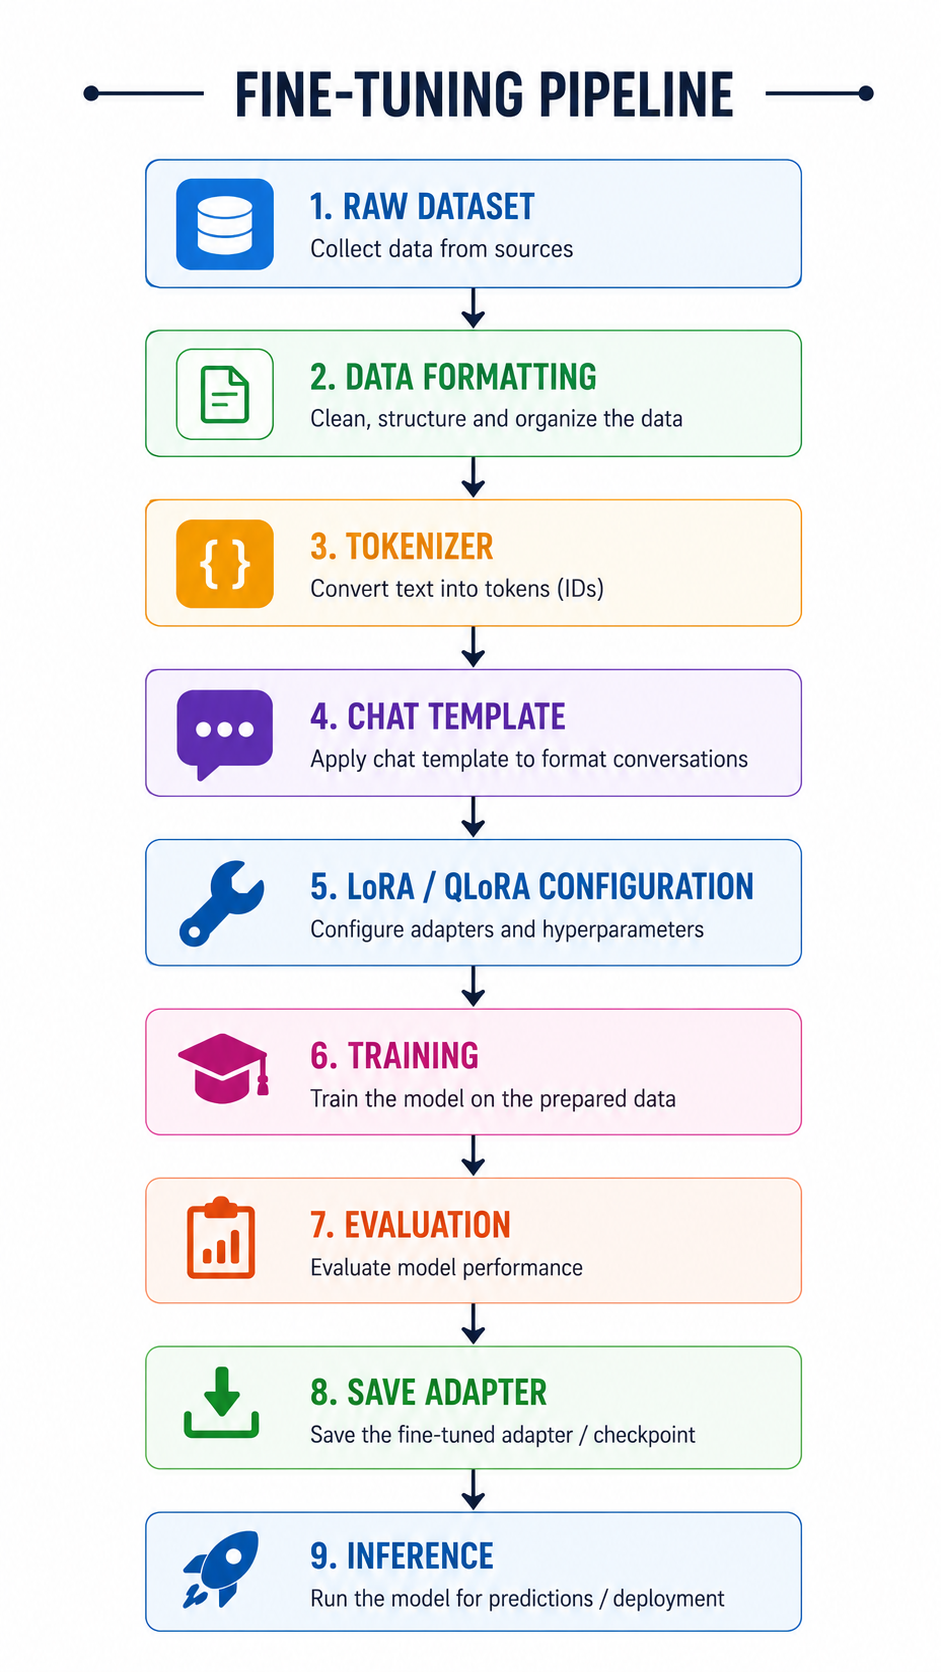
\includegraphics[width=0.85\textwidth]{figures/12-3 figure.png}
\end{figure}


\thispagestyle{empty}

\vspace*{\fill}

\begin{center}

{\Huge\textbf{Thank You}}

\vspace{1.2cm}

{\large
To everyone who opened these pages,\\
explored these ideas, and took the time to learn,\\
question, experiment, and think beyond the familiar.
}

\vspace{0.8cm}

{\large
Whether you are beginning your journey in deep learning\\
or continuing one that has already taken you far,\\
I sincerely hope this book has been a meaningful part of your journey.
}

\vspace{0.8cm}

{\large
Thank you for reading, learning, and being part of this journey\\
\textit{from neurons to intelligence.}
}

\vspace{1.8cm}

{\Large\textbf{Kaddouri Abdelkader}}

\vspace{0.3cm}

{\normalsize Author}

\vspace{1.5cm}

{\small
\textit{The journey of learning never truly ends.}
}

\end{center}

\vspace*{\fill}

\clearpage

\end{document}
